% !TeX root = bccppc.tex

%% abtex2-modelo-trabalho-academico.tex, v<VERSION> laurocesar
%% Copyright 2012-2015 by abnTeX2 group at http://www.abntex.net.br/ 
%%
%% This work may be distributed and/or modified under the
%% conditions of the LaTeX Project Public License, either version 1.3
%% of this license or (at your option) any later version.
%% The latest version of this license is in
%%   http://www.latex-project.org/lppl.txt
%% and version 1.3 or later is part of all distributions of LaTeX
%% version 2005/12/01 or later.
%%
%% This work has the LPPL maintenance status `maintained'.
%% 
%% The Current Maintainer of this work is the abnTeX2 team, led
%% by Lauro César Araujo. Further information are available on 
%% http://www.abntex.net.br/
%%
%% This work consists of the files abntex2-modelo-trabalho-academico.tex,
%% abntex2-modelo-include-comandos and abntex2-modelo-references.bib
%%

% ------------------------------------------------------------------------
% ------------------------------------------------------------------------
% abnTeX2: Modelo de Trabalho Academico (tese de doutorado, dissertacao de
% mestrado e trabalhos monograficos em geral) em conformidade com 
% ABNT NBR 14724:2011: Informacao e documentacao - Trabalhos academicos -
% Apresentacao
% ------------------------------------------------------------------------
% ------------------------------------------------------------------------

\documentclass[
	% -- opções da classe memoir --
	12pt,				% tamanho da fonte
	openright,			% capítulos começam em pág ímpar (insere página vazia caso preciso)
	%twoside,			% para impressão em verso e anverso. Oposto a oneside
  oneside,     % para impressão em verso e anverso. Oposto a twoside
	a4paper,			% tamanho do papel.
 hyphens,
	% -- opções da classe abntex2 --
	chapter=TITLE,		% títulos de capítulos convertidos em letras maiúsculas
	%section=TITLE,		% títulos de seções convertidos em letras maiúsculas
	%subsection=TITLE,	% títulos de subseções convertidos em letras maiúsculas
	%subsubsection=TITLE,% títulos de subsubseções convertidos em letras maiúsculas
	% -- opções do pacote babel --
	english,			% idioma adicional para hifenização
	french,				% idioma adicional para hifenização
	spanish,			% idioma adicional para hifenização
	brazil				% o último idioma é o principal do documento
	]{abntex2}

% ---
% Pacotes básicos 
% ---
%\usepackage{lmodern}			% Usa a fonte Latin Modern
%\usepackage{cfr-lm}      % Technically, lmodern does since the fonts it installs are identical to those used by cfr-lm		
\usepackage[T1]{fontenc}		% Selecao de codigos de fonte.
\usepackage[utf8]{inputenc}		% Codificacao do documento (conversão automática dos acentos)
\usepackage{lastpage}			% Usado pela Ficha catalográfica
\usepackage{indentfirst}		% Indenta o primeiro parágrafo de cada seção.
\usepackage{color}				% Controle das cores
\usepackage{graphicx}			% Inclusão de gráficos
\usepackage{microtype} 			% para melhorias de justificação

%%%%%%%%%%%%%%%%%%%%%%
% pacotes incluídos
\usepackage{longtable}
\usepackage{lscape}
\usepackage{supertabular}

%\usepackage{fontspec}
%\usepackage{fontawesome}
\usepackage{hyperref}
%%%%%%%%%%%%%%%%%%%%%%
% ---



\renewcommand{\ABNTEXchapterfont}{\bfseries}
\renewcommand{\ABNTEXchapterfontsize}{\normalsize}
\renewcommand{\ABNTEXsectionfont}{\bfseries}
\renewcommand{\ABNTEXsectionfontsize}{\normalsize}
\renewcommand{\ABNTEXsubsectionfont}
\renewcommand{\ABNTEXsubsectionfontsize}{\normalsize}

\usepackage{booktabs}

\addto\captionsbrazil{%
  \renewcommand{\tablename}{Quadro}
  \renewcommand{\listtablename}{Lista de quadros}
  }

  \usepackage{multirow}
  \usepackage{enumitem}
  \SetEnumitemKey{midsep}{itemsep=0pt, parsep=0pt}
  \setlist{nosep}

  \usepackage[small]{caption}
% ---
% Pacotes adicionais, usados apenas no âmbito do Modelo Canônico do abnteX2
% ---
\usepackage{lipsum}				% para geração de dummy text
% ---

% ---
% Pacotes de citações
% ---
\usepackage[acronym]{glossaries}

\usepackage[brazilian,hyperpageref]{backref}	 % Paginas com as citações na bibl
\usepackage[alf]{abntex2cite}	% Citações padrão ABNT
\usepackage{url6023}
% --- 
% CONFIGURAÇÕES DE PACOTES
% --- 

% ---
% Configurações do pacote backref
% Usado sem a opção hyperpageref de backref
\renewcommand{\backrefpagesname}{Citado na(s) página(s):~}
% Texto padrão antes do número das páginas
\renewcommand{\backref}{}
% Define os textos da citação
\renewcommand*{\backrefalt}[4]{
	\ifcase #1 %
		Nenhuma citação no texto.%
	\or
		Citado na página #2.%
	\else
		Citado #1 vezes nas páginas #2.%
	\fi}%
% ---

% ---
% Configurações de aparência do PDF final

% alterando o aspecto da cor azul
\definecolor{blue}{RGB}{41,5,195}

% definindo comandos para fontawesome

% \newfontfamily{\FA}{FontAwesome Regular}
% \def\twitter{{\FA \faTwitter}}


% informações do PDF
\makeatletter
\hypersetup{
     	%pagebackref=true,
		pdftitle={\@title}, 
		pdfauthor={\@author},
    	pdfsubject={\imprimirpreambulo},
	    pdfcreator={LaTeX with abnTeX2},
		pdfkeywords={abnt}{latex}{abntex}{abntex2}{trabalho acadêmico}, 
		colorlinks=true,       		% false: boxed links; true: colored links
    	linkcolor=blue,          	% color of internal links
    	citecolor=blue,        		% color of links to bibliography
    	filecolor=magenta,      		% color of file links
		urlcolor=blue,
		bookmarksdepth=4
}
\makeatother
% --- 

% --- 
% Espaçamentos entre linhas e parágrafos 
% --- 

% O tamanho do parágrafo é dado por:
\setlength{\parindent}{1.3cm}

% Controle do espaçamento entre um parágrafo e outro:
\setlength{\parskip}{0.2cm}  % tente também \onelineskip

% ---
% compila o indice
% ---
\makeindex
% ---





\newacronym{abenge}{ABENGE}{Associação Brasileira de Educação em Engenharia}
\newacronym{abnt}{ABNT}{Associação Brasileira de Normas Técnicas}
\newacronym{acc}{ACC}{Atividades Curriculares Complementares}
\newacronym{acei}{ACEI}{Assessoria de Cooperação Internacional}
\newacronym{acg}{ACG}{Avaliação dos Cursos de Graduação}
\newacronym{aee}{AEE}{Atendimento Educacional Especializado}
\newacronym{ava}{AVA}{Ambiente Virtual de Aprendizagem}
\newacronym{avalies}{AVALIES}{Avaliação das Instituições de Ensino Superior}
\newacronym{bcc}{BCC}{Bacharelado em Ciência da Computação}
\newacronym{bext}{BEXT}{Programa Institucional de Bolsas de Extensão}
\newacronym{bia}{BIA}{Bolsa de Incentivo Acadêmico}
\newacronym{came}{CAME}{Coordenação de Acompanhamento e Monitoramento de Egressos}
\newacronym{ccd}{CCD}{Colegiado de Coordenação Didática}
\newacronym{cepe}{CEPE}{Conselho de Ensino, Pesquisa e Extensão}
\newacronym{ces}{CES}{Câmara de Educação Superior}
\newacronym{cfe}{CFE}{Conselho Federal de Educação}
\newacronym{cgcd}{CGCD}{Colegiado Geral de Coordenação Didática}
\newacronym{cne}{CNE}{Conselho Nacional de Educação}
\newacronym{cnpq}{CNPq}{Conselho Nacional de Desenvolvimento Científico Tecnológico}
\newacronym{coaa}{COAA}{Comissão de Orientação e Acompanhamento Acadêmico}
\newacronym{consu}{CONSU}{Conselho Universitário}
\newacronym{cpa}{CPA}{Comissão Própria de Avaliação}
\newacronym{creape}{CREA-PE}{Conselho Regional de Engenharia e Agronomia Pernambuco}
\newacronym{dqv}{DQV}{Departamento de Qualidade de Vida}
\newacronym{ead}{EaD}{Educação a Distância}
\newacronym{enade}{ENADE}{Exame Nacional de Desempenho de Estudantes}
\newacronym{enem}{ENEM}{Exame Nacional do Ensino Médio}
\newacronym{esap}{ESAP}{Escola Superior de Agricultura de Pernambuco}
\newacronym{eso}{ESO}{Estágio Supervisionado Obrigatório}
\newacronym{facepe}{FACEPE}{Fundação de Amparo à Ciência e Tecnologia do Estado de Pernambuco}
\newacronym{ies}{IES}{Instituições de Ensino Superior}
\newacronym{ifes}{IFES}{Institutos Federais de Ensino Superior}
\newacronym{inep}{INEP}{Instituto Nacional de Estudos e Pesquisas Educacionais Anísio Teixeira}
\newacronym{jepex}{JEPEX}{Jornada de Ensino, Pesquisa e Extensão}
\newacronym{la}{LA}{Laboratórios de Acessibilidade}
\newacronym{ldb}{LDB}{Lei de Diretrizes e Bases da Educação Nacional}
\newacronym{libras}{LIBRAS}{Língua Brasileira de Sinais}
\newacronym{mec}{MEC}{Ministério da Educação}
\newacronym{naces}{NACES}{Núcleo de Acessibilidade}
\newacronym{nde}{NDE}{Núcleo Docente Estruturante}
\newacronym{nemam}{NEMAM}{Núcleo de Engenharia e Meio Ambiente}
\newacronym{nuric}{NURIC}{Núcleo de Relações Institucionais e Convênios}
\newacronym{ongs}{ONGs}{Organizações Não Governamentais}
\newacronym{pavi}{PAVI}{Atividade de Vivência Interdisciplinar}
\newacronym{pbl}{PBL}{Project Based Learning}
\newacronym{pdi}{PDI}{Plano de Desenvolvimento Institucional}
\newacronym{pecg}{PEC-G}{Programa de Estudantes-Convênio de Graduação}
\newacronym{pet}{PET}{Programa de Educação Tutorial}
\newacronym{pibic}{PIBIC}{Programa Institucional de Bolsas de Iniciação Científica}
\newacronym{pibiti}{PIBITI}{Programa Institucional de Bolsas de Iniciação em Desenvolvimento Tecnológico e Inovação}
\newacronym{pic}{PIC}{Programa de Iniciação Científica}
\newacronym{pne}{PNE}{Plano Nacional de Educação}
\newacronym{ppc}{PPC}{Projeto Pedagógico do Curso}
\newacronym{ppi}{PPI}{Projeto Pedagógico Institucional}
\newacronym{prae}{PRAE}{Pró-Reitoria de Extensão}
\newacronym{preg}{PREG}{Pró-Reitoria de Ensino de Graduação}
\newacronym{progesti}{PROGESTI}{Pró-Reitoria de Gestão Estudantil e Inclusão}
\newacronym{proplan}{PROPLAN}{Pró-Reitoria de Planejamento, Orçamento e Finanças}
\newacronym{prppg}{PRPPG}{Pró-Reitoria de Pesquisa e Pós-Graduação}
\newacronym{sbc}{SBC}{Sociedade Brasileira de Computação}
\newacronym{siape}{SIAPE}{Sistema Integrado de Administração de Recursos Humanos}
\newacronym{siga}{SIG\@}{Sistema de Informações e Gestão Acadêmica}
\newacronym{sinaes}{SINAES}{Sistema Nacional de Avaliação da Educação Superior}
\newacronym{sisu}{SISU}{Sistema de Seleção Unificado}
\newacronym{tcc}{TCC}{Trabalho de Conclusão de Curso}
\newacronym{tea}{TEA}{Transtorno do Espectro Autista}
\newacronym{tic}{TIC}{Tecnologias de Informação e Comunicação}
\newacronym{uabj}{UABJ}{Unidade Acadêmica de Belo Jardim}
\newacronym{uacsa}{UACSA}{Unidade Acadêmica no Cabo de Santo Agostinho}
\newacronym{uaeadtec}{UAEADTec}{Unidade Acadêmica de Educação a Distância e Tecnologia}
\newacronym{uag}{UAG}{Unidade Acadêmica de Garanhuns}
\newacronym{uast}{UAST}{Unidade Acadêmica de Serra Talhada}
\newacronym{ufape}{UFAPE}{Universidade Federal do Agreste de Pernambuco}
\newacronym{ufpe}{UFPE}{Universidade Federal de Pernambuco}
\newacronym{ufrpe}{UFRPE}{Universidade Federal Rural de Pernambuco}
\newacronym{urp}{URP}{Universidade Rural de Pernambuco}

\makeglossaries

% ----
% Início do documento
% ----


\begin{document}


%%%%%%%%%%%%%%%%%%%%%%%%%%%%%%%%%%%%%%%%%%%%%%
%%%
%%% Capa e Contra-Capa
%%%
%%%%%%%%%%%%%%%%%%%%%%%%%%%%%%%%%%%%%%%%%%%%%%


\begin{center} 
    
\includegraphics[width=2.57cm]{./images/brasao_da_republica.jpeg} \\
    
    Ministério da Educação\\
    Universidade Federal do Agreste de Pernambuco\\
    Pró-Reitoria de Ensino de Graduação
    
          
    \vfill
    % \vspace{4.5cm}
    {{\Large Projeto Pedagógico de Curso}}\\
    \vspace{.5cm}
    {{\Large \textbf{Bacharelado em Ciência da Computação}}}\\
    \vspace{1cm}
    {{\large Perfil: 2.1.0}}\\
    \vfill
    
    %
\includegraphics[width=1cm]{images/uagUFRPE.eps} \\
    
    % {\scshape Pró-Reitoria de Ensino de Graduação\\}
    % {\scshape Unidade Acadêmica de Garanhuns\\}
    % {\scshape Bacharelado em Ciência da Computação\\}
    % Av. Bom Pastor, s/n, Boa Vista, CEP 55292-270, Garanhuns, PE\\
    % Telefone: (87) 3764-5500\\
    % \url{http://bcc.uag.ufrpe.br}\\ \vskip\baselineskip
    
    \vspace{1cm}
    \vskip\baselineskip
    Garanhuns, 2022.
\end{center}

\newpage

%%%%%%%%%%%%%%%%%%%%%%%%%%%%%%%%%%%%%%%%%%%%%%%%%%%%%%%%
%%%
%%% Comissão de Elaboração da Reforma Curricular do Curso
%%%
%%%%%%%%%%%%%%%%%%%%%%%%%%%%%%%%%%%%%%%%%%%%%%%%%%%%%%%%

% \chapter*[Comissão de Elaboração da Reforma Curricular do Curso]{Comissão de Elaboração da Reforma Curricular do Curso}
% \addcontentsline{toc}{chapter}{Comissão de Elaboração da Reforma Curricular do Curso}


% \section*{Elaboração e Edição}

% \noindent Prof. Sérgio Francisco Tavares de Oliveira Mendonça\\
% \noindent  Prof. Gabriel de França Pereira e Silva\\

% \section*{Revisão}

% \noindent Prof. Bruno Costa e Silva Nogueira\\
% \noindent Prof. Célio Andrade de Santana Júnior\\
% \noindent Profa. Maria Aparecida Amorim Sibaldo\\
% \noindent Prof. Rodrigo Gusmão de Carvalho Rocha\\

% \section*{Aprovação}

% \noindent Prof. Alixandre Thiago Ferreira Santana\\
% \noindent Prof. Bruno Costa e Silva Nogueira\\
% \noindent Prof. Célio Andrade de  Santana Júnior\\
% \noindent Profa. Érica Teixeira Gomes de Sousa\\
% \noindent Prof. Fabiano Barbosa Mendes da Silva\\
% \noindent Prof. Gabriel de França Pereira e Silva\\
% \noindent Profa. Juliana de Albuquerque Gonçalves Saraiva\\
% \noindent Profa. Maria Aparecida Amorim Sibaldo\\
% \noindent Prof. Mariel José Pimentel de Andrade\\
% \noindent Prof. Ricardo Normando Baptista do Nascimento Neto\\
% \noindent Prof. Rodrigo Gusmão de Carvalho Rocha\\
% \noindent Prof. Sérgio Francisco Tavares de Oliveira Mendonça\\

% \newpage


%%%%%%%%%%%%%%%%%%%%%%%%%%%%%%%%%%%%%%%%%%%%%%%%%%%%%%%%
%%%
%%% Dados da Criação/Autorização/Reconhecimento do Curso
%%%
%%%%%%%%%%%%%%%%%%%%%%%%%%%%%%%%%%%%%%%%%%%%%%%%%%%%%%%%

% \chapter*[Criação, Autorização e Reconhecimento do Curso]{Criação, Autorização e Reconhecimento do Curso}
% \addcontentsline{toc}{chapter}{Criação, Autorização e Reconhecimento do Curso}

% \begin{itemize}
%   \item Projeto Pedagógico de Curso: Proc. n. 014727/2008-de 01/08/2008;
%   \item Autorização: Art. 35 Decreto 5.773/06 (Redação dada pelo Art. 2 Decreto 6.303/07), Data de Publicação D.O.U: 26/05/2008.
%   \item Reformulação do Projeto Pedagógico de Curso: Proc. n. 018649/2011-de 11/11/2011, Resolução do CEPE n. 005/2012, de 09/01/2012.
%   \item Reconhecimento: Portaria MEC n.649, de 10/12/2013, DOU n. 240, Seção 1, 11/12/2013, ISSN 1677-7042. p. 25-26.
% \end{itemize}

% Com o objetivo de promovermos ampla divulgação e possibilitar a participação ativa (de professores, estudantes, egressos, profissionais e da comunidade em geral) nos princípios norteadores do curso, disponibilizamos as ferramentas de comunicação Fórum (através de email e facebook), além de disponibilizar este Projeto Pedagógico de Curso no Repositório GitHub.

% \begin{itemize}
%   \item Coordenação do Curso (e-mail): \href{mailto:coordenacao.bcc@ufape.edu.br}{coordenacao.bcc@ufape.edu.br}
%   \item Este Projeto no GitHub: \url{https://github.com/ufape/bccppc}
% \end{itemize}

% \vspace{5.5cm}



% \newpage

%%%%%%%%%%%%%%%%%%%%%%%%%%%%%%%%%%%%%%%%%%%%%%
%%%
%%% Identificação do Curso
%%%
%%%%%%%%%%%%%%%%%%%%%%%%%%%%%%%%%%%%%%%%%%%%%%

\chapter*[Dados de Identificação do Curso]{DADOS DE IDENTIFICAÇÃO DO CURSO}
\addcontentsline{toc}{chapter}{Dados de Identificação do Curso}


\begin{center}
  \begin{footnotesize} 
  \begin{longtable}{lp{9.4cm}}
    \caption{\label{quadro:sintese-do-curso}Síntese do curso.}\\
    \toprule
    \multicolumn{2}{c}{\bfseries SÍNTESE DO CURSO} \\
    \midrule
    \textbf{Modalidade} & Presencial \\ \midrule
    \textbf{Denominação do Curso}	& Ciência da Computação \\ \midrule
    \textbf{Habilitação}	& Bacharelado \\ \midrule
    \textbf{Local de Oferta}	& Universidade Federal do Agreste de Pernambuco \newline Av. Bom Pastor, s/n, Boa Vista \newline CEP 55292-270 - Garanhuns/PE \\ \midrule
    \textbf{Turno(s) de Funcionamento}	 & Noturno \\ \midrule
    \textbf{Número de Vagas}	& 80 vagas anuais \\ \midrule
    \textbf{Periodicidade de Oferta}	& Semestral \\ \midrule
    \textbf{Carga Horária Total} & 3.200 horas \\ \midrule
    \textbf{Período de Integralização}	& 4,5 anos (9 semestres) \\ \midrule
    \textbf{Período Máximo de Integralização} 	& 4,5 anos + 70\% desse tempo (15 semestres)\footnote{Resolução UFRPE/CEPE nº 154/2001.} \\ \midrule
    \textbf{Ato Regulatório do Curso} &	Portaria nº 9.222, de 27 de dezembro de 2018. \\ \midrule
    \textbf{Mantida}	& Universidade Federal Rural de Pernambuco UFRPE \newline Pessoa Jurídica de Direito Público - Federal \newline R. Dom Manoel de Medeiros, s/n - Dois Irmãos. Recife - PE \\ \midrule
    \textbf{Corpo Dirigente da UFAPE}	& Nome: Airon Aparecido de Melo \newline Cargo: Reitor \newline Telefone: 0xx(87) 3764-5505 \newline E-mail: airon.melo@ufape.edu.br \\
\bottomrule
\end{longtable}
\end{footnotesize}
\end{center}

\newpage

% Seleciona o idioma do documento (conforme pacotes do babel)
%\selectlanguage{english}
\selectlanguage{brazil}

% Retira espaço extra obsoleto entre as frases.
\frenchspacing 

% ---
% inserir lista de ilustrações
% ---
\pdfbookmark[0]{\listfigurename}{lof}
\listoffigures*
\cleardoublepage
% ---

% ---
% inserir lista de tabelas
% ---
\pdfbookmark[0]{\listtablename}{lot}
\listoftables*
\cleardoublepage
% ---

% ---
% inserir lista de abreviaturas e siglas
% ---
% \begin{siglas}
%   \item[UFRPE] Universidade Federal Rural de Pernambuco
%   \item[UAG] Unidade Acadêmica de Garanhuns
%   \item[BCC] Bacharelado em Ciência da Computação
% \end{siglas}
% % ---


\clearpage

\printglossary[type=\acronymtype, title=Lista de Siglas]

\newpage

% ---
% inserir lista de símbolos
% ---
% \begin{simbolos}
%   \item[$ \Gamma $] Letra grega Gama
%   \item[$ \Lambda $] Lambda
%   \item[$ \zeta $] Letra grega minúscula zeta
%   \item[$ \in $] Pertence
% \end{simbolos}
% ---

% ---
% inserir o sumario
% ---
\pdfbookmark[0]{\contentsname}{toc}
\tableofcontents*
\cleardoublepage
% ---



% ----------------------------------------------------------
% ELEMENTOS TEXTUAIS
% ----------------------------------------------------------
\textual


\chapter*{Apresentação}
\addcontentsline{toc}{chapter}{Apresentação}

Nos dias atuais, o reconhecimento do direito à educação em termos de acesso, permanência e qualidade se faz presente na sociedade brasileira, constituindo em uma agenda de alta prioridade. Neste sentido, as Instituições Públicas de Ensino Superior, fortalecidas pelas políticas afirmativas e inclusivas, vêm contribuindo de maneira expressiva para o desenvolvimento socioeconômico, cultural e tecnológico do país, nas mais variadas áreas do conhecimento humano. É diante dessa conjuntura que a \acrfull{ufape}/\acrfull{ufrpe} reafirma seu compromisso com o desenvolvimento de uma sociedade crítica e participativa através da construção e popularização de saberes científicos, tecnológicos e culturais (UFRPE, 2018).

Atento às demandas sociais, econômicas e culturais do Estado de Pernambuco e, em especial, da Região do Agreste, este \acrfull{ppc} se apresenta como um instrumento político e teórico-metodológico destinado a pautar as práticas acadêmicas do curso de \acrfull{bcc} ofertado pela \acrshort{ufape}, anteriormente, denominada \acrfull{uag}, criada pela Resolução CONSU/UFRPE nº 98/2017.

O curso tem o compromisso de contribuir para a transformação social sustentável, formando profissionais que possam atuar de forma ética e inovadora, respeitando os aspectos legais e as normas inerentes à profissão. Sua concepção está em consonância com a \acrfull{ldb}, as Diretrizes Curriculares Nacionais para a área em questão, bem como o \acrfull{pdi} da \acrshort{ufrpe} e os dispositivos legais da Universidade e Entidades de Classe, como a \acrfull{sbc}. Além disso, sua proposta pedagógica orienta-se por uma \textit{concepção ativa dos processos de ensino e aprendizagem}, incorporando metodologias que incentivam a criatividade e autonomia dos estudantes. Neste sentido, destaca-se o ensino híbrido e a realização de \textit{projetos interdisciplinares} por meio da \textit{\acrlong{pbl}} (\acrshort{pbl}) em diferentes etapas do curso.

Tal como elucida \citeonline{veiga2004educaccao}, o Projeto Pedagógico não representa um documento estanque ou um ``artefato'' meramente técnico. Pelo contrário, devido a sua dinamicidade, ele atua como um mobilizador permanente para todos os agentes envolvidos com o curso: professores, estudantes, técnico-administrativos e gestores. A fim de garantir a formação, este \acrshort{ppc} deverá ser permanentemente acompanhado e avaliado, com vistas à realização do seu aperfeiçoamento e à efetivação da sua intencionalidade.



\chapter{Enquadramento do Curso à Legislação Vigente}

Considerando os dispositivos legais que regulamentam o funcionamento do curso de \acrlong{bcc}, este \acrlong{ppc} foi construído, coletivamente, sob a égide das leis, decretos, resoluções e pareceres, detalhados a seguir, no Quadro~\ref{quadro:base-legal-geral-curso}.


\begin{center}
    
    \begin{scriptsize}
        \begin{longtable}{p{5.8cm}p{9cm}}
            \caption{\label{quadro:base-legal-geral-curso}Base legal geral do curso de \acrlong{bcc}.}\\
    \toprule
    \textbf{Lei, Decreto, Resolução e Parecer} & \textbf{Escopo} \\ 
    \midrule
    Resolução MEC/CNE/CES nº 7/2018 & Dispõe sobre a Curricularização da Extensão--Estabelece que: (1) as atividades de extensão devem compor, no mínimo, 10\% (dez por cento) do total da carga horária curricular estudantil dos cursos de graduação, as quais deverão fazer parte da matriz curricular dos cursos; e (2) instrui o INEP a considerar essas atividades, para efeitos de autorização, reconhecimento e renovação do reconhecimento de cursos, bem como para o credenciamento e recredenciamento das instituições de ensino superior, prevista na Lei nº 13.005/2014--\acrfull{pne}. \\ \midrule
    Portaria MEC nº 1.428/2018	& Dispõe sobre a oferta, por Instituições de Educação Superior--IES, de disciplinas na modalidade a distância em cursos de graduação presencial. \\ \midrule
    Resolução CNE/CES nº 5/2016	& Institui as Diretrizes Curriculares Nacionais para os cursos de graduação na área da Computação, abrangendo os cursos de bacharelado em Ciência da Computação, em Sistemas de Informação, em Engenharia de Computação, em Engenharia de Software e de licenciatura em Computação, e dá outras providências.\\ \midrule
    Lei nº 13.146/2015 & Institui a Lei Brasileira de Inclusão da Pessoa com Deficiência (Estatuto da Pessoa com Deficiência). \\ \midrule
    Lei nº 13.005/2014	& Aprova o \acrshort{pne}. \\ \midrule
    Lei nº 12.764/2012 & Institui a Política Nacional de Proteção dos Direitos da Pessoa com Transtorno do Espectro Autista. \\ \midrule
    Resolução CNE/MEC nº 2/2012 & Estabelece as Diretrizes Curriculares Nacionais para a Educação Ambiental. \\ \midrule
    Resolução CNE/MEC nº 1/2012 & Estabelece Diretrizes Nacionais para a Educação em Direitos Humanos.\\ \midrule
    Parecer CNE/CES nº 136/2012	& Apresenta as Diretrizes Curriculares Nacionais para os cursos de graduação em Computação. \\ \midrule
    Lei nº 11.645/2008	& Altera a Lei nº 9.394, de 20 de dezembro de 1996, modificada pela Lei nº 10.639, de 9 de janeiro de 2003, que estabelece as diretrizes e bases da educação nacional, para incluir no currículo oficial da rede de ensino a obrigatoriedade da temática ``História e Cultura Afro-Brasileira e Indígena''. \\ \midrule
    Resolução CNE/CES nº 2/2007 & Dispõe sobre carga horária mínima e procedimentos relativos à integralização e duração dos cursos de graduação, bacharelados, na modalidade presencial. \\ \midrule
    Parecer CNE/MEC nº 261/2006	& Dispõe sobre procedimentos a serem adotados quanto ao conceito de hora-aula e dá outras providências. \\ \midrule
    Decreto nº 5.626/2005 & Dispõe sobre o Ensino da Língua Brasileira de Sinais--LIBRAS. \\ \midrule
    Decreto nº 5.296/2004 & Estabelece normas gerais e critérios básicos para a promoção da 	acessibilidade das pessoas portadoras de deficiência ou com mobilidade reduzida. \\ \midrule
    Parecer CNE/MEC nº 3/2004 & Apresenta as Diretrizes Curriculares Nacionais para a Educação das	Relações Étnico-Raciais e para o Ensino de História e Cultura Afro-Brasileira e Africana. \\ \midrule
    Resolução CNE/MEC nº 3/2002 & Institui	as Diretrizes Curriculares Nacionais Gerais para a organização e o funcionamento dos cursos superiores de tecnologia. \\ \midrule
    Lei nº 9.795/1999 & Dispõe sobre a educação ambiental, institui a Política Nacional de Educação Ambiental e dá outras providências. \\ \midrule
    Lei nº 9.394/1996 & Estabelece as Diretrizes e Bases da Educação Nacional.\\ 
    \bottomrule
    \end{longtable}
\end{scriptsize}      
\end{center}


Vale ressaltar que, em atendimento à Resolução CNE/MEC nº 1/2012\footnote{\url{http://portal.mec.gov.br/dmdocuments/rcp001_12.pdf}}, a Educação em Direitos Humanos será trabalhada de forma transversal no currículo do curso de \acrlong{bcc}.

Na busca de promover a educação de cidadãos atuantes e conscientes quanto à pluralidade étnico-racial do Brasil, e, considerando o disposto no Parecer CNE/MEC nº~3/2004\footnote{\url{http://portal.mec.gov.br/dmdocuments/cnecp_003.pdf}}, na Resolução CNE/MEC nº 1/2004\footnote{\url{http://portal.mec.gov.br/cne/arquivos/pdf/res012004.pdf}} e na Resolução UFRPE/CEPE nº 217/2012, Art. 2º, será ofertada a disciplina optativa de Educação das Relações Étnico-Raciais para os alunos do curso de \acrlong{bcc}.

A inserção dos conhecimentos concernentes à Educação Ambiental ocorrerá de forma integrada e interdisciplinar, obedecendo a Lei nº 9.795/1999\footnote{\url{http://www.planalto.gov.br/ccivil_03/leis/l9795.htm}}, e a Resolução CNE/MEC nº 2/2012\footnote{\url{http://portal.mec.gov.br/dmdocuments/rcp002_12.pdf}}. Além disso, o curso estará atento às diretrizes dos órgãos e sociedades representativas de suas áreas de atuação profissional, como, por exemplo, a \acrshort{sbc}, que constitui a principal entidade representativa dos profissionais da grande área de computação no Brasil. Destaca-se também que está previsto a oferta da disciplina optativa de Libras, em atendimento ao Decreto no 5.626/2005\footnote{\url{http://www.planalto.gov.br/ccivil_03/_Ato2004-2006/2005/Decreto/D5626.htm}} e a Resolução UFRPE/CEPE nº 030/2010.

Vale salientar que as disciplinas da matriz curricular do curso de \acrlong{bcc} poderão ser ofertadas na modalidade semipresencial/\acrshort{ead}. A oferta destas disciplinas não ultrapassará o percentual de 20\% (vinte por cento) da carga horária total do curso, conforme estabelecido através da Portaria MEC nº 4.059/2004.

Tal como os preceitos outorgados pelos dispositivos legais citados anteriormente, servirão de alicerce para o Curso de \acrlong{bcc} as resoluções internas da \acrshort{ufape} e da \acrshort{ufrpe}, como se observa no Quadro~\ref{quadro:base-legal-ufrpe-curso}, a seguir.

\begin{center}
    
    \begin{scriptsize}
        \begin{longtable}{p{5.8cm}p{9cm}}
            \caption{\label{quadro:base-legal-ufrpe-curso}Base legal da \acrshort{ufape} e \acrshort{ufrpe} que fundamenta o curso.}\\
    \toprule
    \textbf{Resolução} & \textbf{Escopo} \\
    \midrule
    Resolução UFAPE/CONSU \textit{Pro Tempore} 015/2020 & Define e regulamenta critérios para o cômputo das Atividades Curriculares Complementares dos cursos de graduação da Universidade Federal do Agreste de Pernambuco. \\ \midrule
    Resolução UFRPE/CEPE nº 281/2017 & Aprova depósito legal de Monografias e Trabalhos de Conclusão de Cursos de Graduação e Pós-Graduação \textit{Lato Sensu} da UFRPE.\\ \midrule
    Resolução UFRPE/CEPE nº 003/2017 & Aprova alteração das Resoluções UFRPE/CONSU nº 260/2008 e 220/2013, da Universidade Federal Rural de Pernambuco. \\ \midrule
    Resolução UFRPE/CEPE nº 220/2016 & Revoga a Resolução UFRPE/CEPE nº 313/2003, que regulamentava as diretrizes para elaborar e reformular os Projetos Pedagógicos dos Cursos de Graduação da UFRPE e dá outras providências. \\ \midrule
    Resolução UFRPE/CEPE nº 217/2012 & Estabelece a inclusão do componente curricular ``Educação das Relações Étnico-Raciais'', nos currículos dos cursos de graduação da UFRPE. \\ \midrule
    Resolução UFRPE/CEPE nº 065/2011 & Aprova a criação e regulamentação da implantação do Núcleo Docente Estruturante - NDE dos Cursos de Graduação da UFRPE. \\ \midrule
    Resolução UFRPE/CEPE nº 678/2010 & Estabelece normas para organização e regulamentação do Estágio Supervisionado Obrigatório para os estudantes dos cursos de graduação da UFRPE e dá outras providências. \\ \midrule
    Resolução UFRPE/CEPE nº 622/2010 & Regulamenta normas de inserção de notas de avaliação de aprendizagem no Sistema de Informações e Gestão Acadêmica – SIG@ da UFRPE. \\ \midrule
    Resolução UFRPE/CEPE nº 494/2010 & Dispõe sobre a verificação da aprendizagem no que concerne aos Cursos de Graduação. \\ \midrule
    Resolução UFRPE/CEPE nº 425/2010 &	Regulamenta a previsão nos Projetos Pedagógicos de curso da equiparação das atividades de Extensão, Monitorias e Iniciação Científica como Estágios Curriculares. \\ \midrule
    Resolução UFRPE/CEPE nº 030/2010 & Estabelece a inclusão do componente curricular ``LIBRAS'' nos 	currículos dos cursos de graduação da UFRPE. \\ \midrule
    Resolução UFRPE/CEPE nº 597/2009 & Revoga a Resolução UFRPE/CEPE nº 430/2007 e aprova novo Plano de Ensino, dos 	procedimentos e orientações para elaboração, execução e acompanhamento. \\ \midrule
    Resolução UFRPE/CEPE nº 486/2006 & Dispõe sobre obrigatoriedade de alunos ingressos na UFRPE de cursarem os dois primeiros semestres letivos dos cursos para os quais se habilitaram. \\ \midrule
    Resolução UFRPE/CEPE nº 154/2001 & Estabelece critérios para desligamento de alunos da UFRPE por insuficiência de rendimento e decurso de prazo. \\     
    \bottomrule
    \end{longtable}
\end{scriptsize}     
\end{center}

Além das resoluções descritas no Quadro~\ref{quadro:base-legal-ufrpe-curso}, outras normativas institucionais da \acrshort{ufape} e da \acrshort{ufrpe}, serão referenciadas ao longo deste \acrshort{ppc}.



% ----------------------------------------------------------
\chapter{Breve histórico da \acrshort{\MakeLowercase{ufrpe}}/\acrshort{\MakeLowercase{ufape}}}
% ----------------------------------------------------------

A \acrlong{ufrpe} é uma instituição centenária, com atuação proeminente no Estado de Pernambuco e região. Sua história tem início com a criação das Escolas Superiores de Agricultura e Medicina Veterinária do Mosteiro de São Bento, em Olinda, no dia 3 de novembro de 1912. Apenas em fevereiro de 1914 iniciaram-se as aulas na instituição que, por sua vez, funcionava em um prédio anexo ao Mosteiro, sob a direção do abade alemão D. Pedro Roeser. Em dezembro do mesmo ano foi instalado o Hospital Veterinário, sendo este o primeiro do país \cite{melo2010alveitares}. Tendo em vista as limitações de espaço para as aulas práticas do curso de Agronomia, os beneditinos transferiram, em 1917, o referido curso para o Engenho São Bento, localizado no distrito de Tapera, em São Lourenço da Mata.

A década de 1930 foi marcada pela estatização da Instituição, com a desapropriação da Escola Superior de Agricultura de São Bento, em 9 de dezembro de 1936, pela Lei nº 2.443 do Congresso Estadual e Ato nº 1.802 do Poder Executivo Estadual, passando a denominar-se \acrfull{esap}. Pouco mais de um ano depois, através do Decreto nº 82, de 12 de março de 1938, ela foi transferida para o Bairro de Dois Irmãos, no Recife.

Em 1947, através do Decreto Estadual nº 1.741, foram reunidos a \acrshort{esap}, o Instituto de Pesquisas Agronômicas, o Instituto de Pesquisas Zootécnicas e o Instituto de Pesquisas Veterinárias, constituindo, assim, a \acrfull{urp}. Em 1955, através da Lei Federal nº 2.524, a Universidade foi federalizada, passando a fazer parte do Sistema Federal de Ensino Agrícola Superior vinculado ao Ministério da Agricultura. Após a federalização, a \acrshort{urp} elaborou o seu primeiro estatuto, em 1964, com base na \acrshort{ldb} de 1961. Com a promulgação do Decreto Federal nº 60.731, de 19 de maio de 1967, a instituição passou a denominar-se oficialmente \textbf{\acrfull{ufrpe}}.

Em 1957, a Escola Agrotécnica do Nordeste foi incorporada à Universidade passando a ser denominada, a partir de 1968, de Colégio Agrícola Dom Agostinho Ikas (SOUZA, 2000). Atualmente, o Colégio, que também conta com um novo campus em Tiúma, oferece cursos técnicos em Agropecuária (integrado ou não ao Ensino Médio), Alimentos e Administração, além de ofertar outros na modalidade de \acrfull{ead}: Açúcar e Álcool, Alimentos e Administração. Também é destaque sua atuação no âmbito da qualificação profissional, por meio do Programa Nacional de Acesso ao Ensino Técnico e Emprego, tendo formado, desde 2013, mais de 12.000 estudantes em todas as regiões do Estado de Pernambuco.

Na década de 1970, novos cursos de graduação foram criados, sendo eles: Estudos Sociais, Zootecnia, Engenharia de Pesca, Bacharelado e Licenciatura em Ciências Biológicas, Economia Doméstica, Ciências Agrícolas, Engenharia Florestal, Matemática e Química. No mesmo período, a \acrshort{ufrpe} iniciou suas atividades de oferta de curso de pós-graduação \textit{stricto sensu}, com a criação do Mestrado em Botânica, em 1973, por meio de um convênio firmado com a \acrfull{ufpe}.

Os anos de 1980 se destacaram pela reformulação do curso de Licenciatura em Ciências com suas respectivas habilitações. Surgiram, então, quatro novos cursos de Licenciatura Plena: Física, Química, Matemática e Ciências Biológicas.

Nos anos 2000, a \acrshort{ufrpe} vivenciou a expansão de suas atividades com a criação de cursos de graduação (na Sede) e das Unidades Acadêmicas, através do Programa de Reestruturação e Expansão das Universidades Federais. A \acrshort{uag}, localizada no Agreste de Pernambuco, foi a primeira das unidades fundadas pela \acrshort{ufrpe}, tendo iniciado suas atividades no segundo semestre de 2005. A \acrshort{uag} oferta os cursos de Agronomia, Licenciatura em Pedagogia, Letras, Ciência da Computação, Engenharia de Alimentos, Medicina Veterinária e Zootecnia. 
%Destaque-se que a \acrshort{uag} está em processo de emancipação, devendo, em alguns anos, tornar-se uma instituição autônoma. 
Em 2006, no Sertão de Pernambuco, foi criada a \acrfull{uast} que, atualmente, oferta os cursos de Bacharelado em: Administração, Ciências Biológicas, Ciências Econômicas, Sistemas de Informação, além de Engenharia de Pesca, Agronomia, Licenciatura em Letras, Licenciatura em Química e Zootecnia.

Ainda no processo de expansão e inclusão social, em 2005, através do Programa Pró-Licenciatura do \acrfull{mec}, a \acrshort{ufrpe} iniciou as atividades do ensino de graduação na modalidade de \acrshort{ead}. Em 2006, o \acrshort{mec} implantou o Programa Universidade Aberta do Brasil, cuja prioridade foi a formação de profissionais para a Educação Básica. Nesse mesmo ano, a Universidade se engajou no referido programa. Em 2010, foi criada a \acrfull{uaeadtec}, presente em 19 polos nos estados de Pernambuco e Bahia. Sua sede administrativa está localizada no \textit{campus} Dois Irmãos, em Recife. A \acrshort{uaeadtec} oferta oito cursos de graduação: Bacharelado em Administração Pública, Bacharelado em Sistemas de Informação, Licenciatura em Artes Visuais Digitais, Licenciatura em Computação, Licenciatura em Física, Licenciatura em História, Licenciatura em Letras e Licenciatura em Pedagogia.

Ao mesmo tempo em que essa interiorização vem se consolidando com a oferta de cursos presenciais e a distância, a \acrshort{ufrpe} também inovou, em 2014, com a implementação da \acrfull{uacsa}. A referida Unidade tem ofertado tanto cursos Superiores em Tecnologia (Construção Civil, Transmissão e Distribuição Elétrica, Automação Industrial, Gestão da Produção Industrial, Mecânica: Processos Industriais) quanto de Bacharelado em Engenharia (Civil, de Materiais, Elétrica, Eletrônica, e Mecânica).

Em 2017, o \acrfull{consu} da \acrshort{ufrpe}, através da Resolução UFRPE/CONSU nº 098/2017\footnote{\url{http://seg.ufrpe.br/resolucao/res-n\%C2\%BA-0982017}}, aprovou a criação da \acrfull{uabj}, visando atender às demandas de qualificação profissional nas áreas de Engenharia da região. De forma semelhante ao projeto da \acrshort{uacsa}, a \acrshort{uabj} oferta cursos Superiores em Tecnologia (Eletrônica Industrial, Redes de Computadores, Processos Químicos, Gestão de Recursos Hídricos) e de Bacharelado em Engenharia (da Computação, de Controle e Automação, Hídrica, Química).

A \acrshort{ufape} tem sua origem no ano de 2018, a partir da Lei nº 13.651 de 11/04/2018, por desmembramento da \acrshort{ufrpe}. Em seguida, teve início a vigência do Termo de Colaboração Técnica celebrado entre o \acrshort{mec}, por intermédio da Secretaria de Educação Superior, e a \acrshort{ufrpe}, para a implantação da \acrshort{ufape}.

\chapter{Justificativa de oferta do curso}

A computação, inicialmente, foi definida como uma atividade que usa o computador para atingir seu objetivo ou meta. Atualmente, a computação envolve diversas tecnologias com a finalidade de permitir a melhoria da qualidade de vida da sociedade. Assim, a ciência da computação engloba a construção e implementação de projetos de \textit{hardware} e \textit{software} para uma extensa gama de propósitos, processando, estruturando e administrando diversos tipos de sistemas de informação. Portanto, consiste em usar o computador para estudos científicos, construção de uma extensa variedade de tipos de sistemas computacionais, e por conseguinte, ajudar o desenvolvimento tecnológico da sociedade na busca do bem-estar social.

Na \acrshort{ufrpe}, a história da Informática e Computação começa em 1999, quando o Curso de Licenciatura em Computação da \acrshort{ufrpe} foi instituído e teve a primeira oferta de vestibular em 2000. Legalmente, o referido curso encontra-se \textsc{Autorizado}, segundo Resolução UFRPE/CEPE nº 265/1999, implantado segundo Resolução CUNI no. 181/1999, e foi \textsc{Reconhecido} junto ao \acrshort{mec}/\acrshort{inep} em novembro de 2005. O Projeto Pedagógico em vigor encontra-se homologado segundo Resolução CEPE de nº 220/2018. Em dezembro de 2006, foi avaliado pelo \acrshort{mec}/\acrshort{inep}, o qual recebeu o conceito \textsc{Condições Boas}. O curso de Licenciatura em Computação foi criado pois na \acrshort{ufrpe} haviam poucos docentes da área de Computação e a universidade já possuía um consolidado Departamento de Educação. Assim, naquele momento o perfil mais adequado foi o curso de Licenciatura em Computação. Neste cenário, desde o ano 2000 existe na \acrshort{ufrpe} a competência em Informática e Computação e, em 2005, seu quadro docente possuía 6 (seis) doutores em Computação. Hoje, a Computação no Campus de Recife é composto por três cursos:  Licenciatura em Computação; Bacharelado em Ciência da Computação; e, Bacharelado em Sistemas de Informação, bem como dois cursos de pós-graduação, Biometria e Estatística Aplicada, que possui Mestrado e Doutorado, e o curso de Informática Aplicada com Mestrado. 

Atualmente, a \acrshort{ufrpe} possui também a Unidade Acadêmica de Educação à Distância e Tecnologia, ofertando os cursos de Licenciatura em Computação e Bacharelado em Sistemas de Informação em diversos polos espalhados no Nordeste, bem como com projetos de pesquisa aprovados na \acrfull{facepe}. O curso de Licenciatura em Física foi o primeiro projeto de curso na modalidade a distância que foi aprovado conforme a Portaria nº 3.726 em 21/10/2005, publicada no DOU, de 24/10/2005.

Em face deste contexto e pela \textit{expertise} adquirida durante estes anos, a \acrshort{ufrpe} sentiu-se confortável para a criação do Curso de Bacharelado em Ciência da Computação no município de Garanhuns/PE. A primeira turma teve sua entrada em 2009 e foi concluída em 2013. 

O curso de \acrshort{bcc} da \acrshort{ufape} (antes \acrshort{uag}) foi criado em 2008, sob o Art. 35, do Decreto nº 5.773/2006 (Redação dada pelo Art. 2º, do Decreto nº 6.303/2007), com o Projeto Pedagógico de Curso inicial (Processo \acrshort{ufrpe} nº 014727/2008, de 01/08/2008) e, apresentando a sua primeira reformulação através do Processo \acrshort{ufrpe} nº 018649/2011, de 11/11/2011). O curso foi reconhecido através da Portaria \acrshort{mec} nº 649, de 10/12/2013, publicada no DOU nº 240, Seção 1, de 11/12/2013, ISSN 1677-7042. p. 25-26.

A \acrshort{ufape} está situada no Município de Garanhuns, segundo maior da Mesorregião do Agreste Meridional pernambucano, com área de 458.552 km$^2$, população de 138.983 habitantes \cite{ibge2018} e encontra-se a cerca de 230 km da capital Recife, onde fica a Reitoria da \acrshort{ufrpe}.

\section{Contexto de inserção do curso na região}

Além de se configurar como área de entroncamento viário, o Município de Garanhuns centraliza, economicamente, parte da Região Agreste, denominado Agreste Meridional, composta por esse e outros 26 municípios. Devido à  localização  e  à  sua  importância como cidade-polo regional, Garanhuns, historicamente, esteve marcada por sua vocação e perfil atrativo às atividades de comércio e serviços, especialmente ligados às áreas de educação, saúde e turismo.

Segundo a Agência \cite{fidem2017agencia}, a rede de influência de Garanhuns é constituída pelos municípios que estão no entorno da microrregião de Garanhuns e, também, aponta a centralidade da cidade que se consolida como importante cidade-polo comercial e de serviços para o qual se direcionam populações vindas de municípios circunvizinhos, situados no Agreste Meridional, Central e na Mata Sul, conforme pode ser visto na Figura~\ref{fig:centralidade}.


\begin{figure}[!htb]
    \centering
    \caption{\label{fig:centralidade}Centralidade, Área de Influência e Equipamentos Urbanos de Garanhuns}
    
    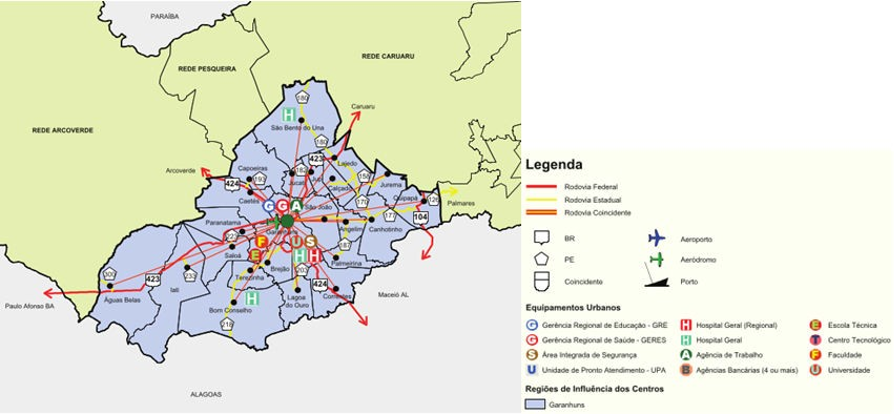
\includegraphics[width=\textwidth]{images/centralidade.png}
    \nota[Fonte]{Agência \cite{fidem2017agencia}}
\end{figure}


A cidade de Garanhuns funciona como uma rede primaz, onde não há outros polos de influência à sua proximidade. Essa rede urbana compreende 7,49\% do território estadual e influencia diretamente 12,43\ dos municípios pernambucanos. O que representa 3,57\% do PIB do Estado, onde o núcleo (Garanhuns) representa 33,57\% do PIB da rede \cite{fidem2017agencia}.

A ideia de criar um curso na área de computação existiu, desde a concepção da UAG, em setembro de 2005, quando começaram a funcionar 4 (quatro) cursos de graduação: Agronomia, Licenciatura Normal Superior (transformada no curso de Licenciatura em Pedagogia), Medicina Veterinária e Zootecnia. Em reunião geral, ocorrida em dezembro de 2007, ficou decidido em processo de votação que seria proposta a criação de 3 (três) novos cursos dentro do processo de Reestruturação Universitária (REUNI). Entre eles foi indicado o curso de \acrlong{bcc}, no turno noturno, com o objetivo tanto de suprir a necessidade de um curso na área de computação, quanto proporcionar o desenvolvimento acadêmico da Universidade mediante uma forte interação com os demais cursos de graduação da Unidade.

Além de interagir com as demais áreas da \acrshort{uag}, o curso de \acrlong{bcc} veio atender a uma demanda regional identificada junto ao poder público local e à população. Portanto, o curso foi inserido dentro do contexto dos demais cursos da área de computação da \acrshort{ufrpe}, de forma a contribuir com o desenvolvimento da \acrshort{uag} e dentro da realidade local. Para tanto, foram definidas áreas de atuação dos profissionais do curso bem como áreas de conhecimento que pudessem ser utilizadas para as outras áreas de conhecimentos já existentes na realidade da \acrshort{ufrpe}/\acrshort{uag}.

De forma paralela, ressaltando a importância da expansão tecnológica, constata-se que o uso do computador deixou de ser um diferencial para se tornar necessidade fundamental, tanto no contexto profissional quanto no dia a dia das pessoas. O advento da \textit{Internet} transformou as tecnologias em elemento chave na construção da chamada sociedade da informação, modificando inclusive a forma de relacionamento na sociedade moderna. Dados de 2016 demonstram que existem, no mundo, cerca de 3.9 bilhões de usuários da \textit{Internet} \cite{sanou2018measuring}, e no Brasil a rede atende a aproximadamente 122 milhões de usuários.

O Brasil sofre com graves problemas tanto no acesso da população aos recursos computacionais quanto nas desigualdades regionais. Junto com a Internet surgem novas oportunidades de desenvolvimento ligadas à produção de conteúdo para a rede, aliados ao desenvolvimento de sistemas que usam grande quantidade de dados. Neste aspecto, é urgente a formação de profissionais ligados ao desenvolvimento de software. Nesse contexto, em 2006, a \acrshort{sbc} definiu cinco grandes desafios atuais da computação:

\begin{enumerate}
    \item Gestão da informação em grandes volumes de dados multimídia distribuídos;
    \item Modelagem computacional de sistemas complexos artificiais, naturais, socioculturais e da interação homem-natureza;
    \item Impactos na computação da transição do silício para novas tecnologias;
    \item Acesso participativo universal do cidadão brasileiro ao conhecimento; e
    \item Sistemas disponíveis, corretos, seguros, escalonáveis, persistentes e ubíquos.
\end{enumerate}
	
Dentro desses desafios, pode-se contextualizar o curso de \acrshort{bcc} da \acrshort{ufape} em uma região carente de profissionais na área de desenvolvimento de software. Além disso, há nessa região, claras possibilidades de aproveitamento dos profissionais a serem formados no ensino superior ofertado em Garanhuns. Com isso, obtêm-se a participação sócio-econômica dos atuais egressos em diferentes áreas técnicas, científicas e informacionais (bacharéis, engenheiros e licenciados) em diversos municípios da região.

Adicionalmente, a região onde se encontra a \acrshort{ufape} tem uma economia com base na agropecuária, e o município de Garanhuns tem uma forte atuação no setor de serviços, com forte apelo para o uso da Computação. Assim, a Computação é também um dos eixos norteadores do desenvolvimento municipal pelo fato do programa de expansão das universidades federais centrar-se na possibilidade de responder às demandas regionais sem, no entanto, restringir-se apenas à região, mas produzindo e transferindo conhecimentos, que é função inerente a toda Universidade. Portanto, o curso de \acrshort{bcc} foi projetado com eixos fundamentados em áreas do conhecimento que viessem a contribuir no desenvolvimento regional.

\section{Resultados obtidos}

Em dezembro de 2015, o curso de \acrshort{bcc} da \acrshort{ufape}, nessa época ainda \acrshort{ufrpe}/\acrshort{uag}, obteve a nota máxima na avaliação do \acrfull{enade}, ou seja, \textsc{Conceito 5/5}. Isso fortaleceu a qualidade e o desempenho dos estudantes, com uma busca contínua da atualização e melhoria dos conteúdos programáticos previstos na diretriz curricular do curso, bem como o desenvolvimento de competências e habilidades necessárias ao aprofundamento da formação geral e profissional, e o nível de atualização dos estudantes com relação à realidade brasileira e mundial.

O curso de \acrshort{bcc} foi avaliado com 4 estrelas (de um máximo de 5), considerado um \textsc{Conceito Muito Bom} nas duas últimas edições da Avaliação de Cursos Superiores do Guia do Estudante (GE) da Editora Abril, nos anos de 2017 e 2018. Essa avaliação consta na publicação GE Profissões Vestibular 2018 e 2019.

O curso hoje é formado por 21 (vinte e um) professores com dedicação exclusiva, distribuídos por formação e atuação nas principais áreas de conhecimento da Ciência da Computação, sendo aproximadamente 18 doutores e 2 mestres (doutorandos). Além disso, também contamos com 4 (quatro) professores das áreas de Matemática, 1 (um) professor da área de Física, 1 (um) professor de Probabilidade e Estatística, 1 (uma) professora de Inglês, e 1 (um) professor de Metodologia da Pesquisa, todos doutores. Atualmente o curso concorre e, frequentemente, é contemplado com bolsas para o desenvolvimento de projetos de pesquisa, extensão e iniciação tecnológica, como também possui grupos de pesquisa e tem gerado diversos artigos publicados por meio de trabalhos realizados com os discentes. Além de artigos, o curso promove melhorias na região por meio dos projetos de extensão que atende a diversas áreas, como projetos interdisciplinares em parceria com os outros cursos. Podemos citar alguns projetos, como: desenvolvimento de aplicativos móveis para auxiliar agricultores e agrônomos nos processos de mecanização agrícola e para o ensino de química básica e avançada; soluções inteligentes para automatizar a irrigação de pequenos produtores rurais da região; ensino de programação básica para alunos de nível médio; e ensino de informática básica para a terceira idade.

O Centro de Tecnologia da Informação do Agreste Meridional de Pernambuco (Time Jr.) é a Empresa Júnior do curso de Bacharelado em Ciência da Computação da \acrshort{ufape}, antiga \acrshort{ufrpe}/\acrshort{uag}. A Time Jr. é uma empresa formal composta por discentes de BCC, sob orientação dos docentes, atuando como desenvolvedora de soluções para as diversas áreas do conhecimento e demanda da sociedade, atuando desde 2012 na região. 

Tomando por base o potencial criador e criativo que a conjuntura local oferece, como curso de Ciência da Computação, demais cursos e sociedade como um todo, e claro, da imensa demanda institucional e local represada, dois projetos foram criados para atuarem nesse cenário,  primeiro Laboratório de Pesquisa e Desenvolvimento, BCC Coworking\footnote{\url{http://bcc.uag.ufrpe.br/bcccoworking}}, que surgiu com o propósito de desenvolvimento de projetos reais, como fomento, com supervisão de profissionais da área, garantindo o conhecimento e a experiência técnica, através do uso de práticas e ferramentas do mercado de trabalho. É um ambiente onde o discente tem a oportunidade trazer sua ideia ou projeto, de criar, manter e aumentar o \textit{networking} com outras pessoas de diversas áreas. É um local para aperfeiçoamento da produtividade. É importante destacar que não se trata de um espaço físico apenas, é principalmente um ambiente destinado aos estudantes em busca de conhecimento, experiência técnica, autonomia, fomentação e desenvolvimento de projetos. 

O segundo Laboratório Multidisciplinar de Tecnologias Sociais\footnote{\url{http://lmts.uag.ufrpe.br/}} (LMTS),  um espaço permanente de ensino, pesquisa, inovação tecnológica, extensão e de colaboração com a gestão institucional, contando com colaboradores da área técnica, mas também das demais áreas citadas, sejam eles, professores, técnicos ou estudantes. Este espaço agrega esta inteligência coletiva e as múltiplas iniciativas em curso ou idealizadas em prol especificamente para o desenvolvimento de \textit{softwares} livres ou públicos para atender as demandas da \acrshort{ufape}, da \acrshort{ufrpe} e da sociedade em geral. O referido laboratório funciona com um propósito sem fins lucrativos, diferentemente da Time Jr. (supracitada) e do BCC Coworking.

Atualmente, no contexto do curso de Ciência da Computação, existem 7 (sete) grupos de pesquisa, liderados e coordenados por professores do curso. Estes grupos atuam nas grandes áreas da computação (Engenharia de Software, Inteligência Artificial, Banco de Dados, Redes de Computadores e Sistemas Distribuídos, Informática e Educação, entre outras) e desenvolvem atividades de ensino, pesquisa, extensão e consultoria/monitoria.

\section{Categorias de cursos da área de computação e informática}

Com as diretrizes curriculares de 1999, foi criada a denominação da área de computação e informática orientando a elaboração do projeto político pedagógico dentro do tipo de curso escolhido. Assim, foram limitadas as possibilidades de nomes de cursos dessa área a 05 (cinco) tipos: Bacharelado em Ciência da Computação, Engenharia da Computação, Bacharelado em Sistemas da Informação, Cursos de Licenciatura em Computação e Cursos Superiores Tecnológicos, e posteriormente, o de Engenharia de Software. Segundo as diretrizes, esses cursos se enquadram em 4 (quatro) categorias básicas:

\begin{enumerate}
    \item Cursos que têm a computação como atividade-fim: Ciência da Computação e Engenharia da Computação;
    \item Cursos que têm a informática como atividade-meio: Sistema da Informação;
    \item Cursos voltados para o ensino da informática: Licenciatura em Computação; e,
    \item Cursos Tecnológicos e sequenciais.
\end{enumerate}

Para que o curso escolhido se inserisse melhor dentro do desenvolvimento da UAG, optou-se pelo curso de Bacharelado em Ciência da Computação (BCC) que se enquadra na categoria de curso com a computação como atividade-fim.

O curso de \acrshort{bcc} da \acrshort{ufape} (na época, \acrshort{uag}) foi idealizado a partir do currículo de referência formulado em documento de 2005 pela IEEE Computer Society, e levando em conta as tendências e desafios para a área de informática descrita em publicação sobre a trajetória dos cursos de graduação da área de computação e informática publicada pela \acrshort{sbc}. A matriz curricular foi construída a partir do estudo de projetos de cursos de de alto nível, outras Instituições de Ensino Superior, seguindo as recomendações do Currículo de Referência da Sociedade Brasileira de Computação (1999) e as diretrizes de 2012 e 2016 do \acrshort{mec}.

Este \acrshort{ppc} vem sendo construído e revisado pelos membros do \acrshort{nde}, com o objetivo de construir um planejamento robusto, e que se torne duradouro. 
%A partir de 2016, com reuniões mensais, uma proposta mais robusta foi sendo consolidada. Essa proposta no decorrer dos anos vem sendo continuamente ajustada e atualizada pelos membros do NDE. Entre as várias dificuldades encontradas pelo NDE para dar prosseguimento ao projeto, as principais foram, realizar um estudo mais profundo para entender e embasar a decisão do curso de se tornar vespertino, como também, mudanças nas resoluções da Sociedade Brasileira da Computação e do Ministério da Educação. E, do ano de 2018 em diante, sofrendo as adequações exigidas pelas Pró-Reitoria de Ensino e Graduação, tendo essa pró-reitoria também enfrentado mudanças nesse período na abordagem de construção dos PPCs.




%%%%%%%%%%%%%%%%%%%%%%%%%%%%%%%%%%%%%%%%%%%%%%%%%%%%%%%%%%%%%%%%%%%%%%%%%%%%%%%%%%%%%
%
% chapter Objetivos do curso
%
%%%%%%%%%%%%%%%%%%%%%%%%%%%%%%%%%%%%%%%%%%%%%%%%%%%%%%%%%%%%%%%%%%%%%%%%%%%%%%%%%%%%%%


\chapter{Objetivos do curso}
\label{cap_objetivos_do_curso}

A Ciência da Computação é uma área de atuação bem diversa, uma vez que o profissional pode atuar em diferentes segmentos, inclusive, apenas na aplicação da computação como meio para outras áreas do conhecimento. O curso de BCC tem como objetivo formar profissionais com bases científicas e tecnológicas na área da computação, capazes de resolver problemas dos mais diferentes domínios, através de métodos e técnicas computacionais, para atuar de forma bem sucedida tanto na área acadêmica quanto no mercado de trabalho. 

Os objetivos específicos do curso são:

\begin{enumerate}
    \item Desenvolver nos estudantes o perfil científico de pesquisador, tanto para atuação na área acadêmica, quanto para atuação em outros ramos de atividade;
    \item Desenvolver nos estudantes um espírito empreendedor, incentivando e motivando a sua independência e criatividade;
    \item Desenvolver nos discentes o perfil para trabalhar na indústria, aplicando os seus conhecimentos técnicos de desenvolvimento de software e soluções para TI;
    \item Promover a interdisciplinaridade buscando atualização constante na área de computação;
    \item Motivar e orientar o estudante para que ele tenha uma postura ativa diante da necessidade de um aprendizado contínuo e autônomo;
    \item Promover uma postura ética e socialmente comprometida com o papel do estudante no desenvolvimento científico, tecnológico, social e econômico da sua região e do País;
    \item Promover interação constante com escolas do ensino fundamental e médio local, de forma a estimular vocações e colaborar ativamente com a melhoria da educação.
    
\end{enumerate}




%%%%%%%%%%%%%%%%%%%%%%%%%%%%%%%%%%%%%%%%%%%%%%%%%%%%%%%%%%%%%%%%%%%%%%%%%%%%%%%%%%%%%
%
% chapter Perfil profissional do egresso
%
%%%%%%%%%%%%%%%%%%%%%%%%%%%%%%%%%%%%%%%%%%%%%%%%%%%%%%%%%%%%%%%%%%%%%%%%%%%%%%%%%%%%%%



\chapter{Perfil profissional do egresso}
\label{cap_perfil_profissional_egresso}

Deve se interessar pela computação e, em particular, pela ciência. Deve possuir entusiasmo para conhecer e dominar novos assuntos, além de disposição para construir sua própria reputação por meio dos produtos do esforço próprio ou resultantes de trabalho em equipe do qual participa. Deve possuir atitude e a necessidade de realizar, mesmo sem supervisão. Deve engajar-se em representações locais, regionais, nacionais e internacionais, através de representações de classe, visando a atualização e fortalecimento da sociedade.

\section{Descrição dos requisitos psicofísicos}

Para atender ao perfil profissional definido, as atividades do curso priorizam o exercício dos requisitos inerentes ao desempenho da profissão, a citar:

\begin{itemize}
    \item Método e disciplina de trabalho;
    \item Raciocínio lógico e abstrato;
    \item Capacidade de trabalho em equipe;
    \item Criatividade, produtividade e iniciativa;
    \item Disposição para efetuar trabalho complexo e minucioso;
    \item Compromisso com o desenvolvimento tecnológico;
    \item Compromisso com o ser humano;
    \item Senso crítico, seriedade e responsabilidade.
\end{itemize}

\section{Egresso}

Do egresso de um curso de Bacharelado em Ciência da Computação é exigida uma predisposição e aptidões para a área, além de um conjunto de competências, habilidades e atitudes a serem adquiridas durante a realização do curso.  Dessa maneira, espera-se que os egressos desse curso:

\begin{enumerate}
    \item Possuam sólida formação em Ciência da Computação e Matemática, que os capacitem a construir aplicativos de propósito geral, ferramentas e infraestrutura de software de sistemas de computação e de sistemas embarcados, gerar conhecimento científico e inovação, e que os incentivem a estender suas competências à medida que a área se desenvolve;
    \item Adquiram visão global e interdisciplinar de sistemas e entendam que esta visão transcende os detalhes de implementação dos vários componentes e os conhecimentos dos domínios de aplicação;
    \item Conheçam a estrutura dos sistemas de computação e os processos envolvidos na sua construção e análise;
    \item Dominem os fundamentos teóricos da área de Computação e como eles influenciam a prática profissional;
    \item Sejam capazes de agir de forma reflexiva na construção de sistemas de computação, compreendendo o seu impacto direto ou indireto sobre as pessoas e a sociedade;
    \item Sejam capazes de criar soluções, individualmente ou em equipe, para problemas complexos caracterizados por relações entre domínios de conhecimento e de aplicação.
\end{enumerate}

\section{Definição do perfil profissional}

Por definição, o Bacharel em Ciência da Computação deve ser um profissional qualificado para a pesquisa e desenvolvimento na área de computação, para o projeto e construção de hardware e software básico e também para o uso de sistemas computadorizados em outras áreas da atividade humana, a fim de viabilizar ou aumentar a produtividade e a qualidade de todos os tipos de procedimentos. Na UFRPE todo egresso deve ser um profissional: (1) com domínio e capacidade para trabalhar na área da Computação, desenvolvendo projetos de computadores e sistemas de computação, programas e sistemas de informação; (2) atento ao caráter ecológico, social e ético; e (3) que exerça suas atividades na sociedade com responsabilidade.

Adaptadas de documentos propostos pela ACM/IEEE e SBC, seguem as competências e habilidades necessárias para o egresso profissional de Ciência da Computação:

\begin{itemize}
    \item Possuir capacidade de raciocínio lógico e abstrato;
    \item Capacidade de utilizar conhecimentos de matemática, física, ciência da computação, engenharia e tecnologias modernas no apoio à construção de produtos e serviços seguros, confiáveis e de relevância social;
    \item Identificar práticas apropriadas dentro de um quadro ético, legal e profissional;
    \item Capacidade de atuar profissionalmente com ética avaliando o impacto de suas atividades no contexto social e ambiental;
    \item Reconhecer a necessidade de um desenvolvimento profissional contínuo;
    \item Capacidade para aprender a aprender. O profissional precisará estar sempre aprendendo para se manter atualizado e competente. A habilidade em pesquisa está fortemente relacionada com o auto-aprendizado;
    \item Discutir e explicar aplicações baseadas no corpo de conhecimento da computação;
    \item Visão sistêmica da área de computação;
    \item Profundo conhecimento dos aspectos teóricos, científicos e tecnológicos relacionados à área de computação;
    \item Demonstrar habilidade para trabalhar como um indivíduo sob orientação, como um membro de uma equipe ou como líder de uma equipe;
    \item Eficiência na operação de equipamentos computacionais e sistemas de software;
    \item Competência para identificar, analisar e documentar oportunidades, problemas e necessidades passíveis de solução via computação, e para empreender na concretização desta solução;
    \item Capacidade para pesquisar e viabilizar soluções de software para várias áreas de conhecimento e aplicação, como por exemplo, desenvolvimento e/ou aprimoramento de protocolos de comunicação, modelos matemáticos-computacionais, técnicas de armazenamento de dados, construção de linguagens de programação, dentre inúmeras outras;
    \item Capacidade de abstração quando desenvolvendo as atividades de programação, projeto e modelagem;
    \item Compreender e aplicar conceitos, princípios e práticas essenciais no contexto de cenários bem definidos, mostrando discernimento na seleção e aplicação de técnicas e ferramentas;
    \item Compreensão da importância de se valorizar o  usuário  no  processo  de  interação com sistemas computacionais e competência na utilização de técnicas de interação homem-máquina neste processo;
    \item Conhecimento de aspectos relacionados à evolução da área de computação, de forma a poder compreender a situação presente e projetar a evolução futura;
    \item Capacidade para desenvolvimento de pesquisa científica e tecnológica, que permita ao aluno ingressar em um curso de pós-graduação ou realizar estas pesquisas na indústria;
    \item Capacidade de avaliar de forma aprofundada e com embasamento teórico as atividades realizadas e produtos desenvolvidos. Esta habilidade pode ser desenvolvida através de atividades de leitura e discussão de temas e elaboração de painéis de discussão com profissionais da área;
    \item Capacidade para conceber soluções inovadoras para tornar produtos competitivos;
    \item Capacidade de, com base nos conceitos adquiridos, iniciar, projetar, desenvolver, implementar, validar e gerenciar qualquer projeto de software. Este trabalho exige habilidade de solução de problemas e de avaliação crítica;
    \item Capacidade para projetar e desenvolver sistemas que integram hardware e software;
    \item Capacidade para avaliar prazos e custos em projetos de software;
    \item Competência e compromisso com a utilização de princípios e ferramentas que reduzam o tempo de desenvolvimento e implementação de um projeto e lhe confiram um alto grau de qualidade;
    \item Aplicação eficiente dos princípios de gerenciamento, organização e busca de informações;
    \item Conhecimento de aspectos relacionados às tecnologias de mídias digitais;
    \item Habilidade de lidar com notações, linguagens e ferramentas para elaboração de modelos;
    \item Capacidade empreendedora, inclusive para aqueles que não desejam ser empresários. Esta habilidade capacita o profissional a tomar iniciativas e a liderar projetos em suas atividades profissionais. Ela é desenvolvida nos alunos através de projetos nos quais eles são estimulados a apresentar e liderar projetos de sistemas;
    \item Capacidade de se expressar bem de forma oral ou escrita usando a língua portuguesa através da elaboração e apresentação de projetos e monografias durante todo o curso;
    \item Fluência na língua inglesa suficiente para a leitura e compreensão de documentos técnicos na área de computação. O egresso deve desenvolver competência e desempenho em língua inglesa através de disciplinas complementares e leitura de livros e artigos de computação escritos em Inglês, que são exigidos em várias atividades curriculares. 
\end{itemize}





%%%%%%%%%%%%%%%%%%%%%%%%%%%%%%%%%%%%%%%%%%%%%%%%%%%%%%%%%%%%%%%%%%%%%%%%%%%%%%%%%%%%%
%
% chapter Campo de Atuação Profissional
%
%%%%%%%%%%%%%%%%%%%%%%%%%%%%%%%%%%%%%%%%%%%%%%%%%%%%%%%%%%%%%%%%%%%%%%%%%%%%%%%%%%%%%%


\chapter{Campo de atuação profissional}
\label{cap_campo_de_atuacao_profissional}

Na contemporaneidade tem-se exigido respostas céleres a problemas complexos decorrentes do mundo globalizado, no qual a informação adquire um papel proeminente. Não é por acaso que o atual modo de vida das pessoas está intrinsecamente ligado ao uso das tecnologias, em especial, dos computadores. Estes podem ser encontrados nos mais variados lugares, como, por exemplo, nos lares (em TV's, eletrodomésticos, vídeo games), escolas (PC's, tablets, laboratórios), indústria (equipamentos de segurança, relógios-ponto, máquinas), comércio (caixas registradoras), dentre outros. 

Desta forma, o profissional atuará possivelmente nos seguintes problemas:

\begin{itemize}
    \item Concepção, especificação, projeto, construção, avaliação e adaptação de sistemas digitais;
    \item Análise e projeto de estrutura lógica e funcional de computadores e sua implementação;
    \item Desenvolvimento e implementação de software básico e de apoio para sistemas computacionais;
    \item Projeto e desenvolvimento de sistemas e programas usando linguagens de programação;
    \item Projeto e desenvolvimento de sistemas de estruturação de informação;
    \item Projeto e desenvolvimento de redes de processamento local e remota, em matéria de hardware e de software.    
\end{itemize}

O egresso do curso de Bacharelado em Ciência da Computação deve estar preparado para propor soluções inovadoras e adequadas para problemas propostos, capacitado a acompanhar e avaliar avanços tecnológicos em computação, bem como aplicar e implementar as evoluções, reposições e adaptações que se façam necessárias, tanto de forma reativa como pró-ativa, logo deve estar apto a desenvolver as seguintes funções no mercado de trabalho:

\begin{itemize}
    \item \textbf{Empreendedor} – descobrimento e empreendimento de novas oportunidades para aplicações usando sistemas computacionais e avaliando a conveniência de se investir no desenvolvimento da aplicação;
    \item \textbf{Consultor} – consultoria e assessoria a empresas de diversas áreas no que tange ao uso adequado de sistemas computacionais;
    \item \textbf{Coordenador de equipe} – coordenação de equipes envolvidas em projetos na área de computação e informática;
    \item \textbf{Membro de equipe} – participação de forma colaborativa e integrada de equipes que desenvolvem projetos na área de informática;
    \item \textbf{Pesquisador} – participação em projetos de pesquisa científica e tecnológica. 
\end{itemize}




%%%%%%%%%%%%%%%%%%%%%%%%%%%%%%%%%%%%%%%%%%%%%%%%%%%%%%%%%%%%%%%%%%%%%%%%%%%%%%%%%%%%%
%
% chapter Requisitos de Ingresso
%
%%%%%%%%%%%%%%%%%%%%%%%%%%%%%%%%%%%%%%%%%%%%%%%%%%%%%%%%%%%%%%%%%%%%%%%%%%%%%%%%%%%%%%


\chapter{Requisitos de ingresso}

O curso de Bacharelado em Ciência da Computação tem duas entradas anuais com 40 vagas por semestre letivo, resultando em 80 vagas por ano. O ingresso dos alunos ocorre através do \acrfull{sisu}, com base nos resultados obtidos no \acrfull{enem}, e do Ingresso Extra.

\begin{enumerate}
    \item \textbf{Ingresso através do \acrshort{enem}}: A \acrshort{ufape} adota o \acrshort{sisu} como principal meio de acesso aos cursos de graduação, através da nota do \acrshort{enem}, considerando as duas entradas semestrais.
    \item \textbf{Ingresso Extra}: Além do ingresso semestral, a partir da seleção do \acrshort{sisu}, a \acrshort{ufape} possui outras modalidades de acesso. Estas ocorrem duas vezes por ano, em datas previstas e com editais publicados pela \acrfull{preg}. 
\end{enumerate}

Nessa direção, são modalidades de ingresso extra:

\begin{itemize}
    \item \textbf{Reintegração} – Após ter perdido o vínculo com a Universidade, o aluno que tenha se evadido pelo período máximo de integralização de seu curso poderá requerer a reintegração, uma única vez, no mesmo curso (inclusive para colação de grau), desde que tenha condições de concluí-lo no prazo máximo permitido (considerando o prazo do vínculo anterior e o que necessitará para a integralização do currículo) e que não possua 4 (quatro) ou mais reprovações em uma mesma disciplina (Fundamentação: Resolução UFRPE/CEPE nº 100/1983, de 16/09/1983; e, Resolução UFRPE/CEPE nº 354/2008, de 13/06/2008).
    \item \textbf{Reopção ou Transferência Interna} – O aluno regularmente matriculado que esteja insatisfeito com o seu curso poderá requerer a transferência interna para outro curso de graduação desta Universidade. Para tanto, ele deverá considerar: a área de conhecimento afim ao seu curso de origem; a existência de vagas no curso pretendido; o cumprimento de, no mínimo, 40\% (quarenta por cento) do currículo original do seu curso, dispondo, portanto, de tempo para integralização curricular, considerando os vínculos com o curso anterior e o pretendido (Fundamentação: Resolução UFRPE/CEPE nº 34/97, de 16/01/1997).
    \item \textbf{Transferência Externa} – A Universidade recebe alunos de outras IES, vinculados a cursos reconhecidos pelo \acrfull{cne}, desde que eles: desejem continuar o curso iniciado ou ingressar em curso de área afim; estejam com vínculo ativo ou trancado com a Instituição de origem; tenham condições de integralizar o currículo no seu prazo máximo, considerando, também, o prazo definido pela outra IES e o que necessitaria cursar na \acrshort{ufape}; e, por fim, que tenham cursado todas as disciplinas constantes do primeiro período da matriz curricular do curso pretendido na \acrshort{ufape}. Salvo os casos de transferência \textit{ex officio} (que independem de vagas), é necessário, para ingresso, que o curso tenha vagas ociosas (Fundamentação: Res. UFRPE/CEPE nº 124/1983 e 180/1991).
    \item \textbf{Portadores de Diploma de Curso Superior} – Os portadores de diploma de curso superior, reconhecido pelo \acrshort{cne}, que desejem realizar matrícula em outro curso superior na \acrshort{ufape}, em área afim, podem requerê-la desde que haja disponibilidade após o preenchimento de vagas pelas demais modalidades de ingresso. (Fundamentação: Resolução UFRPE/CEPE nº 181/1991, de 01/10/1991).
\end{itemize}

As formas de ingresso definidas a seguir independem de vagas e não há necessidade de publicação de edital da \acrshort{preg}:

\begin{itemize}
    \item \textbf{Cortesia Diplomática} – Em atendimento ao que preconiza o Decreto nº 89.758/1984, de 06/06/1984, a \acrshort{ufape} aceita alunos incluídos nas seguintes situações: funcionário estrangeiro, de missão diplomática ou repartição consular de carreira no Brasil, e seus dependentes legais; funcionário estrangeiro de Organismo Internacional que goze de privilégios e imunidades em virtude de acordo entre o Brasil e a organização, e seus dependentes legais; técnico estrangeiro, e seus dependentes legais, que preste serviço em território nacional, no âmbito de acordo de cooperação cultural, técnica, científica ou tecnológica, firmado entre o Brasil e seu país de origem, desde que em seu contrato esteja prevista a permanência mínima de 1 (um) ano no Brasil; e, finalmente, técnico estrangeiro, e seus dependentes legais, de organismo internacional, que goze de privilégios e imunidades em virtude de acordo entre o Brasil e a organização, desde que em seu contrato esteja prevista a permanência mínima de 1 (um) ano em território nacional.

    Este tipo de ingresso nos cursos de graduação se dá mediante solicitação do Ministério das Relações Exteriores, encaminhada pelo \acrshort{mec}, com a isenção de processo seletivo e independentemente da existência de vagas, sendo, todavia, somente concedido a estudantes de países que assegurem o regime de reciprocidade e que sejam portadores de visto diplomático ou oficial.

    \item \textbf{Programa de Estudantes-Convênio de Graduação (PEC-G)} – Alunos provenientes de países em desenvolvimento, especialmente da África e da América Latina, são aceitos como estudantes dos cursos de graduação da \acrshort{ufrpe}. Estes estudantes são selecionados, por via diplomática em seus países, considerando os mecanismos previstos no protocolo do PEC-G e obedecendo aos princípios norteadores da filosofia desse Programa. Não pode ser admitido, através desta modalidade, o estrangeiro portador de visto de turista, diplomático ou permanente, bem como o brasileiro dependente dos pais que, por qualquer motivo, estejam prestando serviços no exterior, e o indivíduo com dupla nacionalidade, sendo uma delas brasileira.
    \item {\bfseries Transferência Obrigatória ou \textit{ex officio}} – É a Transferência definida na Lei n.º 9.536, de 11/12/1997 que regulamenta o Art. 49 da Lei n.º 9.394, de 20/12/1996, Portaria Ministerial nº 975/1992, de 25/06/92 e Resolução nº 12, de 02/07/1994 do \acrfull{cfe}. Esta transferência independe da existência de vaga e época, abrangendo o servidor público federal da administração direta ou indireta, autárquica, fundacional ou membro das Forças Armadas, regidos pela Lei n.º 8.112/1990, inclusive seus dependentes, quando requerido em razão de comprovada remoção ou transferência \textit{ex officio}. A transferência deverá implicar em mudança de residência para o município onde se situe a instituição recebedora ou para localidade próxima a esta, observadas as normas estabelecidas pelo \acrshort{cne}.
\end{itemize}





%%%%%%%%%%%%%%%%%%%%%%%%%%%%%%%%%%%%%%%%%%%%%%%%%%%%%%%%%%%%%%%%%%%%%%%%%%%%%%%%%%%%%
%
% chapter Organização Curricular
%
%%%%%%%%%%%%%%%%%%%%%%%%%%%%%%%%%%%%%%%%%%%%%%%%%%%%%%%%%%%%%%%%%%%%%%%%%%%%%%%%%%%%%%


\chapter{Organização curricular}

Levando em consideração as orientações contidas na Resolução CNE/CES nº 5 de 11/2016, que institui as Diretrizes Curriculares Nacionais para os cursos de graduação na área da Computação, o currículo do curso de \acrshort{bcc} apresenta a estrutura conforme Quadro~\ref{quadro:organizacao-curricular-do-curso}:

\begin{center}
    \begin{scriptsize}
      \begin{longtable}{@{}lp{10cm}}
        \caption{\label{quadro:organizacao-curricular-do-curso}Organização curricular do curso.}\\
      \toprule
      \textbf{Núcleo de Conhecimento} & \textbf{Componentes Curriculares} \\ 
      \midrule
        Conteúdos Básicos 
                                & CÁLCULO PARA COMPUTAÇÃO I \\
                                & GEOMETRIA ANALÍTICA A\\
                                & LÓGICA MATEMÁTICA \\
                                & CÁLCULO PARA COMPUTAÇÃO II \\
                                & FÍSICA PARA COMPUTAÇÃO \\ 
                                & ÁLGEBRA LINEAR I \\
                                & PROBABILIDADE E ESTATÍSTICA \\
                                & METODOLOGIA CIENTÍFICA \\
                                & MATEMÁTICA DISCRETA \\
                                & INGLÊS  \\
                                \midrule
        Conteúdos Tecnológicos
                                & INTRODUÇÃO À PROGRAMAÇÃO \\
                                & INTRODUÇÃO À COMPUTAÇÃO C \\
                                & ALGORITMOS E ESTRUTURA DE DADOS I\\
                                & PROGRAMAÇÃO ORIENTADA AO OBJETO \\
                                & SISTEMAS DIGITAIS \\
                                & ALGORITMOS E ESTRUTURA DE DADOS II \\
                                & ARQUITETURA DE COMPUTADORES \\
                                & PROJETO E ANÁLISE DE ALGORITMOS \\
                                & ENGENHARIA DE SOFTWARE \\
                                & PARADIGMAS DE LINGUAGENS DE PROGRAMAÇÃO \\
                                & BANCO DE DADOS I\\
                                & SISTEMAS DE INFORMAÇÃO E TECNOLOGIAS \\
                                & SISTEMAS OPERACIONAIS \\
                                & INTELIGÊNCIA ARTIFICIAL \\
                                & TEORIA DA COMPUTAÇÃO \\
                                & REDES DE COMPUTADORES \\
                                & COMPUTAÇÃO GRÁFICA \\
                                & COMPILADORES \\
                                & RECONHECIMENTO DE PADRÕES \\
                                & EMPREENDEDORISMO I\\
                                & SISTEMAS DISTRIBUÍDOS \\
                                & PROJETO DE DESENVOLVIMENTO DE SOFTWARE \\
                                & INTERAÇÃO HUMANO-COMPUTADOR \\
                                & COMPUTADORES E SOCIEDADE \\
                                & ESTÁGIO SUPERVISIONADO OBRIGATÓRIO \\
                                & TRABALHO DE CONCLUSÃO DE CURSO\\
      \bottomrule
      \end{longtable}
    \end{scriptsize}      
  \end{center}

A carga horária total do curso de \acrlong{bcc} tem um total de 3.200 (três mil e duzentas) horas, distribuídas entre componentes curriculares obrigatórios e optativos, em 4,5 (quatro vírgula cinco) anos, em 9 (nove) semestres (ou períodos). Os conteúdos de formação serão apresentados em componentes curriculares com carga horária variando entre 30 (trinta) e 60 (sessenta) horas para as disciplinas, 300 (trezentas) horas para \acrshort{eso} e 180 (cento e oitenta) horas para \acrshort{tcc}. Cada hora-aula corresponde a 60 (sessenta) minutos, conforme expresso na Resolução UFRPE/CEPE nº~220/2016 e demonstrado no Quadro~\ref{quadro:distribuicao-nucleos-formacao-e-ch}.

  \begin{center}
    
    \begin{scriptsize}
      \begin{longtable}{p{4cm}p{1.5cm}p{2cm}p{3cm}}
        \caption{\label{quadro:distribuicao-nucleos-formacao-e-ch}Distribuição dos núcleos de formação e carga horária.}\\
      \toprule
      \multicolumn{4}{c}{\textbf{\acrlong{bcc}}}\\ \midrule
      \multicolumn{2}{l}{\textbf{Núcleo}} & \multicolumn{1}{c}{\textbf{Carga Horária (h)}} & \multicolumn{1}{c}{\textbf{\%}}\\
      \midrule
      Básicos & & \multicolumn{1}{c}{540} & \multicolumn{1}{r}{16,9}\\ \midrule
      \multirow{3}{3cm}{Tecnológico / Profissionalizante} & Disciplinas & \multicolumn{1}{c}{1.440} & \multicolumn{1}{r}{45,0}\\ \cline{2-4}
      & TCC & \multicolumn{1}{c}{180} & \multicolumn{1}{r}{5,6}\\ \cline{2-4}
      & ESO & \multicolumn{1}{c}{300} & \multicolumn{1}{r}{9,4}\\ \midrule
      \multicolumn{2}{l}{Componentes optativos} & \multicolumn{1}{c}{420} & \multicolumn{1}{r}{13,1}\\ \midrule
      \multicolumn{2}{l}{Atividades curriculares complementares} & \multicolumn{1}{c}{320} & \multicolumn{1}{r}{10,0}\\ \midrule
      \multicolumn{2}{l}{Total} & \multicolumn{1}{c}{3.200} & \multicolumn{1}{r}{100,0}\\
  \bottomrule
  \end{longtable}
  \end{scriptsize}      
  \end{center}
  
  Para obtenção do título em Bacharel em Ciência da Computação o aluno deverá cumprir uma carga horária total de 3.200 (três mil e duzentas) horas, entre disciplinas, atividades curriculares complementares, trabalho de conclusão de curso e estágio obrigatório supervisionado. O discente terá a possibilidade de cursar disciplinas do ciclo básico e disciplinas do ciclo tecnológico/profissionalizante, podendo ainda escolher em qual área deseja se aprofundar, uma vez que pode escolher entre as disciplinas optativas que necessita cursar.
  
  As disciplinas de um mesmo período letivo ou de períodos anteriores, no qual o aluno tenha cursado, devem se articular em torno de um ou mais projetos de natureza interdisciplinar, buscando otimizar o processo de avaliação nas disciplinas e uma melhor adequação do esforço para resolução de problemas por parte dos discentes, uma vez que assim eles concentram seus esforços num único projeto que contempla aquelas disciplinas que naturalmente interagem. As disciplinas, em suas atividades e projetos, são baseadas na metodologia \acrshort{pbl} \cite{barrows1986taxonomy}). Além do diálogo entre as disciplinas, o curso estará atento à tentativa de promoção de uma educação inclusiva, adaptando os conteúdos programáticos previstos em cada componente curricular em função das necessidades de aprendizagem dos estudantes.
  
  Algumas disciplinas serão ofertadas de forma semipresencial, atendendo as exigências do MEC do Art. 7º, da Portaria nº 1.428/2018, cujos métodos e práticas de ensino-aprendizagem incorporarão \acrfull{tic} para a realização dos objetivos pedagógicos, e pode ser observado no Capítulo~\ref{cap_metodologia_e_avaliacao} Metodologia e Avaliação.
  
  Com relação a carga horária permitida para as disciplinas na modalidade semipresencial, atualmente o curso atende o percentual máximo de 20\% (vinte por cento) da carga horária total do curso ou das disciplinas no formato \acrshort{ead}, consoante a Portaria \acrshort{mec} nº 1.134/2016 e Resolução UFRPE/CEPE nº 220/2016. Porém, algumas disciplinas poderão ser ofertadas com até o percentual de 20\% (vinte por cento) na modalidade a distância, conforme a portaria nº 4.059/2004 do \acrshort{mec}, desde que sejam apresentados os programas de disciplinas, métodos, formas de avaliação e acompanhamento e a justificativa.
  
  O desenvolvimento de atividades práticas e visitas técnicas a organizações públicas, privadas e não governamentais, permitirá aos estudantes o contato com demandas e situações próprias da profissão. Esta, também incluirá, como etapa integrante da graduação, o \acrshort{eso}, sob a orientação direta da instituição de ensino, conforme disposto no Capítulo~\ref{cap_eso}. A carga horária do \acrshort{eso} será de 300 (trezentas) horas. Será obrigatório, ainda, o desenvolvimento do \acrshort{tcc} com 180 (cento e oitenta) horas. A participação no \acrfull{enade} é requisito indispensável para a integralização do curso, bem como a integralização de 420 (quatrocentas e vinte) horas de disciplinas optativas. E, a integralização de 320 (trezentas e vinte) horas de Atividades Curriculares Complementares.
  
  \section{Matriz curricular}
  
  A matriz curricular busca atender os objetivos traçados e o perfil desejado do egresso em Ciência da Computação. Os componentes curriculares que serão ofertados no bacharelado estão distribuídos considerando a seguinte tipologia: Obrigatórios (que corresponde àquelas que o aluno deve obrigatoriamente cursar ao longo dos semestres) e optativos (dentre o rol de disciplinas ofertadas, o aluno escolhe cursar aquelas de seu interesse). No Quadro~\ref{quadro:matriz-curricular-do-curso} a seguir são expostos os períodos nos quais estes componentes estão dispostos no curso.
  
  \begin{center}
    
    \begin{tiny}
      \begin{longtable}{cp{4.5cm}cccp{2.8cm}p{2.8cm}}
        \caption{\label{quadro:matriz-curricular-do-curso}Matriz Curricular do curso de Ciência da Computação.}\\
      \toprule
      \textbf{Per.} & \textbf{Disciplina} & \multicolumn{3}{c}{\textbf{Carga Horária}} & \textbf{Pré-requisitos} & \textbf{Correquisitos}\\
      & & \textbf{Teó.} & \textbf{Prát.} & \textbf{Total} & & \\
      \midrule
      1 
        & CÁLCULO PARA COMPUTAÇÃO I & 60 & 0 & 60 & & \\ \cline{2-7}
        & GEOMETRIA ANALÍTICA A & 60 & 0 & 60 & & \\ \cline{2-7}
        & LÓGICA MATEMÁTICA & 60 & 0 & 60  & &\\ \cline{2-7}
        & INTRODUÇÃO À PROGRAMAÇÃO & 45 & 45 & 90  & &\\ \cline{2-7}
        & INTRODUÇÃO À COMPUTAÇÃO C & 30 & 0 & 30  & &\\ \midrule
        & \multicolumn{3}{l}{\textbf{Subtotal}} & \textbf{300} & & \\ \midrule
      2 
        & CÁLCULO PARA COMPUTAÇÃO II & 60 & 0 & 60 & CÁLCULO I & \\ \cline{2-7}   
        & FÍSICA PARA COMPUTAÇÃO & 60 & 0 & 60 & CÁLCULO I & \\ \cline{2-7}
        & ÁLGEBRA LINEAR I & 60 & 0 & 60 & GEOMETRIA ANALÍTICA & \\ \cline{2-7}
        & ALGORITMOS E ESTRUTURA DE DADOS I & 30 & 30 & 60 & INTRODUÇÃO À PROGRAMAÇÃO & \\  \cline{2-7}
        & PROGRAMAÇÃO ORIENTADA AO OBJETO & 30 & 30 & 60 & INTRODUÇÃO À PROGRAMAÇÃO & \\ \midrule
        & \multicolumn{3}{l}{\textbf{Subtotal}} & \textbf{300} & & \\ \midrule
    3 
        & PROBABILIDADE E ESTATÍSTICA & 60 & 0 & 60 & CÁLCULO II & \\ \cline{2-7}
        & SISTEMAS DIGITAIS & 45 & 15 & 60 & & \\ \cline{2-7}
        & METODOLOGIA CIENTÍFICA & 30 & 0 & 30 & & \\ \cline{2-7}
        & MATEMÁTICA DISCRETA PARA COMPUTAÇÃO & 60 & 0 & 60 & LÓGICA MATEMÁTICA & \\ \cline{2-7}
        & ALGORITMOS E ESTRUTURA DE DADOS II & 30 & 30 & 60 & ALGORITMOS E ESTRUTURA DE DADOS I & \\ \cline{2-7}
        & INGLÊS & 30 & 0 & 30  & &\\ \midrule
        & \multicolumn{3}{l}{\textbf{Subtotal}} & \textbf{300} & & \\ \midrule
    4 
        & ARQUITETURA DE COMPUTADORES & 45 & 15 & 60 & SISTEMAS DIGITAIS; \newline FÍSICA PARA COMPUTAÇÃO & \\ \cline{2-7}
        & PROJETO E ANÁLISE DE ALGORITMOS & 30 & 30 & 60 & ALGORITMOS E ESTRUTURA DE DADOS II & \\ \cline{2-7}
        & ENGENHARIA DE SOFTWARE & 30 & 30 & 60 & PROGRAMAÇÃO ORIENTADA A OBJETOS & \\ \cline{2-7}
        & PARADIGMAS DE LINGUAGENS DE PROGRAMAÇÃO & 45 & 15 & 60 & INTRODUÇÃO À PROGRAMAÇÃO; \newline ALGORITMOS E ESTRUTURA DE DADOS I; \newline ALGORITMOS E ESTRUTURA DE DADOS II & \\ \cline{2-7}
        & BANCO DE DADOS & 30 & 30 & 60 & & \\ \cline{2-7}
        & \multicolumn{3}{l}{\textbf{Subtotal}} & \textbf{300} & & \\ \midrule
    5 
        & SISTEMAS DE INFORMAÇÃO E TECNOLOGIAS & 60 & 0 & 60 & ENGENHARIA DE SOFTWARE & \\ \cline{2-7}
        & SISTEMAS OPERACIONAIS & 45 & 15 & 60 & ARQUITETURA DE COMPUTADORES; \newline SISTEMAS DIGITAIS; \newline FÍSICA PARA COMPUTAÇÃO; \newline CÁLCULO PARA COMPUTAÇÃO I & \\ \cline{2-7}
        & INTELIGÊNCIA ARTIFICIAL & 30 & 30 & 60 & INTRODUÇÃO À PROGRAMAÇÃO; \newline ALGORITMOS E ESTRUTURA DE DADOS I; \newline ALGORITMOS E ESTRUTURA DE DADOS II; \newline PROJETO E ANÁLISE DE ALGORITMOS; \newline PARADIGMAS DE LINGUAGENS DE PROGRAMAÇÃO; \newline LÓGICA MATEMÁTICA & \\ \cline{2-7}
        & TEORIA DA COMPUTAÇÃO & 60 & 0 & 60 & & \\ \cline{2-7}
        & REDE DE COMPUTADORES & 30 & 30 & 60 & INTRODUÇÃO À COMPUTAÇÃO C; \newline INTRODUÇÃO À COMPUTAÇÃO; \newline ALGORITMOS E ESTRUTURA DE DADOS I \newline ALGORITMOS E ESTRUTURA DE DADOS II & \\ \midrule
        & \multicolumn{3}{l}{\textbf{Subtotal}} & \textbf{300} & & \\ \midrule
    6 
        & COMPUTAÇÃO GRÁFICA & 30 & 30 & 60 & INTRODUÇÃO À PROGRAMAÇÃO; \newline ÁLGEBRA LINEAR; \newline GEOMETRIA ANALÍTICA A & \\ \cline{2-7}
        & COMPILADORES & 45 & 15 & 60 & TEORIA DA COMPUTAÇÃO; \newline ALGORITMOS E ESTRUTURAS DE DADOS II & \\ \cline{2-7}
        & RECONHECIMENTO DE PADRÕES & 60 & 0 & 60 & ALGORITMOS E ESTRUTURA DE DADOS II; \newline MATEMÁTICA DISCRETA; \newline LÓGICA MATEMÁTICA & COMPUTAÇÃO GRÁFICA \\ \cline{2-7}
        & EMPREENDEDORISMO & 60 & 0 & 60 & & \\ \cline{2-7}
        & SISTEMAS DISTRIBUÍDOS & 30 & 30 & 60 & SISTEMAS OPERACIONAIS; \newline REDE DE COMPUTADORES; \newline INTRODUÇÃO À COMPUTAÇÃO C & \\ \midrule 
        & \multicolumn{3}{l}{\textbf{Subtotal}} & \textbf{300} & & \\ \midrule
    7 
        & PROJETO DE DESENVOLVIMENTO & 30 & 30 & 60 & ENGENHARIA DE SOFTWARE; \newline ENGENHARIA DE SOFTWARE; \newline INTRODUÇÃO À PROGRAMAÇÃO & \\ \cline{2-7}
        & INTERAÇÃO HU\-MA\-NO-COM\-PU\-TA\-DOR & 30 & 30 & 60 & ENGENHARIA DE SOFTWARE & \\ \cline{2-7}
        & COMPUTADORES E SOCIEDADE & 15 & 15 & 30  & &\\ \cline{2-7}
        & OPTATIVA I & & & 60 & & \\ \cline{2-7}
        & OPTATIVA II & & & 60 & & \\ \midrule
        & \multicolumn{3}{l}{\textbf{Subtotal}} & \textbf{300} & & \\ \midrule
    8
        & OPTATIVA III & & & 60 & & \\ \cline{2-7}
        & OPTATIVA IV & & & 60 & & \\ \cline{2-7}
        & OPTATIVA V & & & 60 & & \\ \cline{2-7}
        & OPTATIVA VI & & & 60 & & \\ \cline{2-7}
        & OPTATIVA VII & & & 60 & & \\ \midrule
        & \multicolumn{3}{l}{\textbf{Subtotal}} & \textbf{300} & & \\ \midrule
    9   
        & ESTÁGIO SUPERVISIONADO OBRIGATÓRIO & 0 & 300 & 300 & & \\ \cline{2-7}
        & TRABALHO DE CONCLUSÃO DE CURSO - CIÊNCIA DA COMPUTAÇÃO & 0 & 180 & 180 & & \\ \midrule
        & \multicolumn{3}{l}{\textbf{Subtotal}} & \textbf{480} & & \\ \midrule
        & \multicolumn{3}{l}{\textbf{Carga Horária Total}} & \textbf{2.880} & & \\
      \bottomrule
  \end{longtable}
  \end{tiny}      
  \end{center}
  
  \subsection{Síntese dos componentes curriculares optativos}
  
  O elenco de componentes curriculares optativos previstos para o curso serão detalhados no Quadro~\ref{quadro:sintese-componentes-curriculares-optativos}, com a indicação de suas cargas horárias e de seus respectivos pré-requisitos, nos quais os discentes deverão cursar no mínimo 420 (quatrocentas e vinte) horas em disciplinas optativas.
  
  \begin{center}
    
    \begin{tiny}
      \begin{longtable}{p{2.5cm}p{5.5cm}cccp{3.3cm}}
        \caption{\label{quadro:sintese-componentes-curriculares-optativos}Síntese dos componentes curriculares optativos.}\\
      \toprule
      \multicolumn{6}{c}{\textbf{Grupo/Área de Conhecimento}} \\ \midrule
      \textbf{Área} & \textbf{Disciplina} & \multicolumn{3}{c}{\textbf{Carga Horária}} & \textbf{Pré-requisitos} \\
      & & \textbf{Teó.} & \textbf{Prát.} & \textbf{Total} & \\
      \midrule
    Banco de Dados & ADMINISTRAÇÃO DE BANCO DE DADOS & 30 & 30 & 60 & BANCO DE DADOS \\ \cline{2-6}
      & CCMP3091 INTEGRAÇÃO DE DADOS E DATA WAREHOUSE & 30 & 30 & 60 & BANCO DE DADOS \\ \cline{2-6}
      & MINERAÇÃO DE DADOS & 30 & 30 & 60 & BANCO DE DADOS \\ \cline{2-6}
      & MODELAGEM CONCEITUAL DE DADOS & 30 & 30 & 60 & BANCO DE DADOS \\ \cline{2-6}
      & SISTEMAS DE INFORMAÇÃO GEOGRÁFICAS & 30 & 30 & 60 & BANCO DE DADOS \\ \cline{2-6}
      & PESQUISA EM GERENCIAMENTO DE DADOS & 30 & 30 & 60 & BANCO DE DADOS \\ \cline{2-6}
      & UAG00169 TÓPICOS ESPECIAIS EM BANCO DE DADOS & 30 & 30 & 30 & BANCO DE DADOS \\ \midrule
    Engenharia da Computação & UAG00304 AVALIAÇÃO DE DESEMPENHO DE SISTEMAS & 30 & 30 & 60 & ALGORITMOS E ESTRUTURAS DE DADOS II \\ \cline{2-6}
      & PROJETO DE SISTEMAS EMBARCADOS & 30 & 30 & 60 & ARQUITETURA E ORGANIZAÇÃO DE COMPUTADORES \\ \cline{2-6}
      & UAG00043 PROTOTIPAÇÃO DE CIRCUITOS DIGITAIS & 30 & 30 & 60 & SISTEMAS DIGITAIS \\ \cline{2-6}
      & SISTEMAS DE TEMPO REAL & 30 & 30 & 60 & SISTEMAS OPERACIONAIS \\ \midrule
      Engenharia de Software & UAG00031 TESTE DE SOFTWARE & 30 & 30 & 60 & ENGENHARIA DE SOFTWARE \\ \cline{2-6}
      & ESPECIFICAÇÃO FORMAL DE SOFTWARE & 30 & 30 & 60 & MATEMÁTICA DISCRETA \\ \cline{2-6}
      & PROGRAMAÇÃO COMPETITIVA & 20 & 40 & 60 & - \\ \cline{2-6}
      & PROGRAMAÇÃO WEB & 30 & 30 & 60 & - \\ \cline{2-6}
      & PROGRAMAÇÃO ORIENTADA A OBJETOS II & 30 & 30 & 60 & PROGRAMAÇÃO ORIENTADA À OBJETOS \\ \cline{2-6}
      & CCMP3078 DESENVOLVIMENTO DE APLICAÇÕES MÓVEIS & 30 & 30 & 60 & ENGENHARIA DE SOFTWARE \\ \cline{2-6}
      & CCMP3051 DESENVOLVIMENTO DISTRIBUÍDO DE SOFTWARE & 45 & 15 & 60 & ENGENHARIA DE SOFTWARE \\ \cline{2-6}
      & ESTIMATIVAS E MEDIÇÃO DE SOFTWARE & 15 & 15 & 30 & ENGENHARIA DE SOFTWARE \\ \cline{2-6}
      & METODOLOGIAS ÁGEIS & 45 & 15 & 60 & ENGENHARIA DE SOFTWARE \\ \cline{2-6}
      & CCMP3080 TÓPICOS ESPECIAIS EM ENGENHARIA DE SOFTWARE & 60 & 0 & 60 & ENGENHARIA DE SOFTWARE \\ \midrule
    Inteligência Computacional & ALGORITMOS DE APRENDIZAGEM DE MÁQUINA & 15 & 15 & 30 & - \\ \cline{2-6}
      & MÁQUINA DE VETORES DE SUPORTE & 15 & 15 & 30 & - \\ \cline{2-6}
      & PROJETO EM APRENDIZAGEM DE MÁQUINA & 15 & 75 & 90 & - \\ \cline{2-6}
      & RECONHECIMENTO DE PADRÕES & 45 & 15 & 60 & APRENDIZAGEM DE MÁQUINA \\ \cline{2-6}
      & REDUÇÃO DE DIMENSIONALIDADE EM APRENDIZAGEM DE MÁQUINA & 15 & 45 & 60 & - \\ \cline{2-6}
      & CCMP3086 TÓPICOS ESPECIAIS EM INTELIGÊNCIA ARTIFICIAL & 30 & 30 & 60 & INTELIGÊNCIA ARTIFICIAL \\ \cline{2-6}
      & REDES NEURAIS ARTIFICIAIS & 15 & 45 & 60 & - \\ \cline{2-6}
      & APRENDIZAGEM DE MÁQUINA BAYESIANA & 15 & 15 & 30 & - \\ \cline{2-6}
      & UAG00011 VISÃO COMPUTACIONAL & 45 & 15 & 60 & PROCESSAMENTO DIGITAL DE IMAGENS \\ \midrule
    Matemática Computacional & ÁLGEBRA LINEAR II & 60 & 0 & 60 & ÁLGEBRA LINEAR I \\ \cline{2-6}
      & CÁLCULO III & 60 & 0 & 60 & CÁLCULO II \\ \cline{2-6}
      & CÁLCULO IV & 60 & 0 & 60 & CÁLCULO III \\ \cline{2-6}
      & CÁLCULO LAMBDA & 60 & 0 & 60 & MATEMÁTICA DISCRETA \\ \cline{2-6}
      & INTRODUÇÃO À COMPUTAÇÃO QU NTICA & 30 & 30 & 60 & TEORIA DA COMPUTAÇÃO \\ \cline{2-6}
      & OTIMIZAÇÃO COMBINATÓRIA (META-HEURÍSTICAS) & 30 & 30 & 60 & PROJETO DE ANÁLISE DE ALGORITMOS \\ \cline{2-6}
      & PESQUISA OPERACIONAL & 30 & 30 & 60 & PROJETO DE ANÁLISE DE ALGORITMOS \\ \cline{2-6}
      & TEORIA DOS NÚMEROS E CRIPTOGRAFIA & 60 & 0 & 60 & MATEMÁTICA DISCRETA \\ \cline{2-6}
      & MATM3017 CÁLCULO NUMÉRICO E COMPUTACIONAL & 60 & 0 & 60 & CÁLCULO II \\ \cline{2-6}
      & MÉTODOS COMPUTACIONAIS DE OTIMIZAÇÃO & 60 & 0 & 60 & CÁLCULO II \\ \cline{2-6}
      & INTRODUÇÃO À CRIPTOGRAFIA E SEGURANÇA DA INFORMAÇÃO & 30 & 30 & 60 & - \\ \cline{2-6}
      & TÓPICOS EM MODELAGEM MATEMÁTICA CONTINUA & 60 & 0 & 60 & CÁLCULO II \\ \cline{2-6}
      & ÁLGEBRA LINEAR COMPUTACIONAL & 60 & 0 & 60 & ÁLGEBRA LINEAR \\ \midrule
    Mídia e Interação 
    & PROCESSAMENTO DIGITAL DE IMAGEM & 30 & 30 & 60 & ALGORITMOS E ESTRUTURA DE DADOS II \\ \cline{2-6}
    & REALIDADE VIRTUAL E AUMENTADA & 30 & 30 & 60 & COMPUTAÇÃO GRÁFICA \\ \cline{2-6}
      & CCMP3076 TÓPICOS ESPECIAIS EM PROCESSAMENTO DE SINAIS & 30 & 30 & 60 & CÁLCULO II E ÁLGEBRA LINEAR \\ \cline{2-6}
      & CCMP3088 TÓPICOS ESPECIAIS EM MÍDIA E INTERAÇÃO & 30 & 30 & 60 & - \\ \midrule
    Redes e Sistemas Distribuídos & GERENCIAMENTO DE REDES DE COMPUTADORES & 30 & 30 & 60 & REDES DE COMPUTADORES \\ \cline{2-6}
      & INFRAESTRUTURA DE REDES E CABEAMENTO ESTRUTURADO & 30 & 30 & 60 & REDES DE COMPUTADORES \\ \cline{2-6}
      & TÓPICOS ESPECIAIS EM REDES DE COMPUTADORES E SISTEMAS DISTRIBUÍDOS & 30 & 30 & 60 & SISTEMAS DISTRIBUÍDOS \\ \cline{2-6}
      & CCMP3079 SEGURANÇA DE REDES DE COMPUTADORES & 30 & 30 & 60 & REDES DE COMPUTADORES \\ \cline{2-6}
      & MODELAGEM DE DEPENDABILIDADE  & 30 & 30 & 60 & PROBABILIDADE E ESTATÍSTICA \\ \midrule
    Informática na Educação & DESENVOLVIMENTO DE SOFTWARE EDUCACIONAL & 30 & 30 & 60 & - \\ \cline{2-6}
      & EDUC3048 INFORMÁTICA NA EDUCAÇÃO & 30 & 30 & 60 & - \\ \cline{2-6}
      & TECNOLOGIAS ASSISTIVAS & 30 & 30 & 60 & - \\ \cline{2-6}
      & TECNOLOGIAS, COGNIÇÃO E APRENDIZAGEM & 30 & 30 & 60 & - \\ \midrule
    Tecnologia da Informação & UAG00080 GESTÃO DA TECNOLOGIA DA INFORMAÇÃO & 60 & 0 & 60 & SISTEMAS DE INFORMAÇÃO E TECNOLOGIAS \\ \cline{2-6}
      & CCMP3077 GESTÃO DE SERVIÇOS EM TI & 60 & 0 & 60 & SISTEMAS DE INFORMAÇÃO E TECNOLOGIAS \\ \cline{2-6}
      & UAG00079 GOVERNANÇA EM TECNOLOGIA DA INFORMAÇÃO & 60 & 0 & 60 & SISTEMAS DE INFORMAÇÃO E TECNOLOGIAS \\ \cline{2-6}
      & CCMP3083 TÓPICOS ESPECIAIS EM GESTÃO DE PROJETOS & 60 & 0 & 60 & SISTEMAS DE INFORMAÇÃO E TECNOLOGIAS \\ \cline{2-6}
      & UAG00300 FUNDAMENTOS EM CIÊNCIA DE DADOS & 60 & 0 & 60 & BANCO DE DADOS \\ \cline{2-6}
      & UAG00300 GESTÃO DE PROCESSOS DE NEGÓCIO & 60 & 0 & 60 & SISTEMAS DE INFORMAÇÃO E TECNOLOGIAS \\ \midrule
    Libras & EDUC3090 LIBRAS & 30 & 30 & 60 & - \\ \midrule
    Educação das Relações Étnico\-Racial & EDUC3092  EDUCAÇÃO DAS RELAÇÕES ÉTNICO-RACIAIS & 60 & 0 & 60 & - \\
  \bottomrule
  \end{longtable}
  \end{tiny}      
  \end{center}
  
  \subsection{Síntese da carga horária total do curso}
  
  No Quadro~\ref{quadro:sintese-carga-horaria-total-do-curso} abaixo, observa-se a síntese da carga horária total do curso.
  
  
  \begin{center}
    
    \begin{tiny}
      \begin{longtable}{lccc}
        \caption{\label{quadro:sintese-carga-horaria-total-do-curso}Síntese da carga horária total do curso.}\\
      \toprule
      \textbf{Detalhamento da CH} & \textbf{Carga Horária} & \textbf{Créditos} & \textbf{Percentual da CH total}\\
      \midrule
      Disciplinas Obrigatórias & 1.980 & 132 & 61,9\% \\ \midrule
      Disciplinas Optativas & 420 & 28 & 13,1\% \\ \midrule
      ESO & 300 & 20 & 9,4\% \\ \midrule
      TCC & 180 & 12 & 5,6\% \\ \midrule
      Atividades Curriculares Complementares & 320 & 21 & 10,0\% \\ \midrule
      Total & 3.200 & 213 & 100,0\% \\
  \bottomrule
  \end{longtable}
  \end{tiny}      
  \end{center}
  
  \section{Representação gráfica da matriz curricular}
  
  Segue a representação gráfica da matriz curricular do curso de BCC, de forma que é possível entender e visualizar melhor o sequenciamento lógico entre as disciplinas e seus períodos.
  
  \begin{figure}[!htb]
    \centering
    \caption{\label{fig:matriz-curricular}Matriz Curricular.}
    
    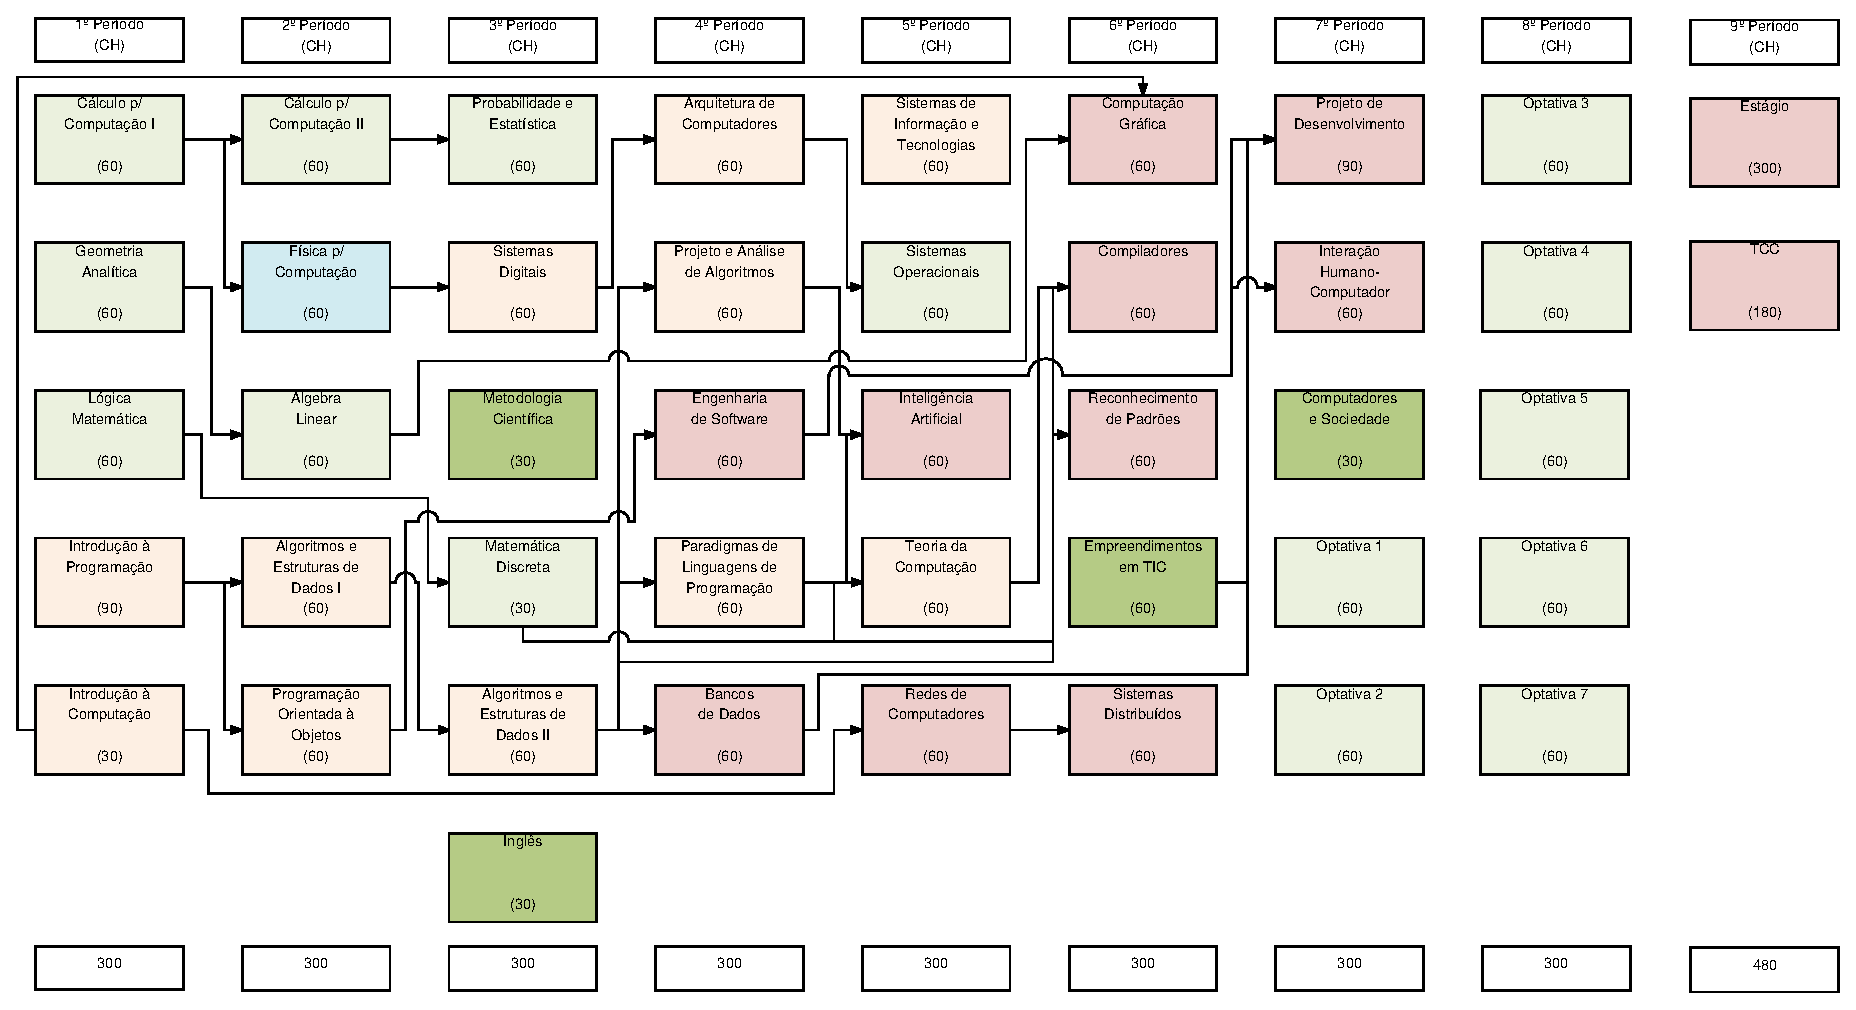
\includegraphics[width=\textwidth]{./images/matriz6.eps}
  \end{figure}
  




  \section{Quadro de Equivalência}
  
  Diante da necessidade de adequar o perfil curricular do curso de Bacharelado em Ciência da Computação, os alunos que ingressarão no curso a partir do semestre letivo de 2021.1 deverão compulsoriamente seguir a nova Matriz Curricular. Já os alunos que ingressaram em períodos anteriores ao semestre supracitado poderão, desde que atendam aos critérios definidos pelo \acrfull{ccd} do curso, optar por seguir a antiga matriz curricular ou fazer a transição para a nova, buscando a equivalência de disciplinas entre as duas matrizes, conforme se mostra os Quadros~\ref{quadro:disciplinas-obrigatorias-equivalentes} e \ref{quadro:disciplinas-optativas-equivalentes}. 
  
  \begin{center}
    
    \begin{tiny}
      \begin{longtable}{p{6.5cm}cp{6.5cm}c}
        \caption{\label{quadro:disciplinas-obrigatorias-equivalentes}Disciplinas Obrigatórias Equivalentes.}\\
      \toprule
      \textbf{PPC2013 Perfil: 2.0.0} & \textbf{CH} & \textbf{PPC2022 Perfil: 2.1.0} & \textbf{CH}\\
      \midrule
      MATM3031 CÁLCULO PARA COMPUTAÇÃO I  & 60 & CÁLCULO I & 60 \\ \midrule
      ADMT3018 EMPREENDIMENTOS EM TIC & 60 & BCC00003 EMPREENDEDORISMO & 60 \\ \midrule
      MATM3032 CÁLCULO PARA COMPUTAÇÃO II  & 60 & CÁLCULO II & 60 \\ \midrule
      MATM3019 ÁLGEBRA LINEAR  & 60 & ÁLGEBRA LINEAR I & 60 \\ \midrule
      CCMP3059 MATEMÁTICA DISCRETA  & 60 & MATEMÁTICA DISCRETA PARA COMPUTAÇÃO & 60 \\ \midrule
      CCMP3066 BANCO DE DADOS I & 60 & BANCO DE DADOS & 60 \\ \midrule
      CCMP3069 PROJETO DE DESENVOLVIMENTO & 90 & PROJETO DE DESENVOLVIMENTO DE SOFTWARE & 60 \\
  \bottomrule
  \end{longtable}
  \end{tiny}
  \end{center}
  
  É importante salientar que o estudante que optar em realizar o processo de migração de perfil curricular do curso, não poderá solicitar retorno para o perfil de origem (antigo). Como pode ser observado pelo quadro de equivalências entre componentes curriculares das diferentes matrizes, o aluno que migrar para o novo perfil curricular poderá aproveitar as disciplinas já cursadas, incluindo as disciplinas optativas de acordo com o Quadro 9 abaixo.
  
  \begin{center}
    
    \begin{tiny}
      \begin{longtable}{p{2cm}p{5.4cm}cp{5.4cm}c}
        \caption{\label{quadro:disciplinas-optativas-equivalentes}Disciplinas Optativas Equivalentes.}\\
      \toprule
      \textbf{Área} & \textbf{PPC2013 Perfil: 2.0.0} & \textbf{CH} & \textbf{PPC2022 Perfil: 2.1.0} & \textbf{CH}\\
      \midrule
    Banco de Dados & - & & ADMINISTRAÇÃO DE BANCO DE DADOS & 60 \\ \cline{2-5}
      & CCMP3091 INTEGRAÇÃO DE DADOS E DATA WAREHOUSE & 60 & INTEGRAÇÃO DE DADOS E DATA WAREHOUSE & 60 \\ \cline{2-5}
      & - & & MINERAÇÃO DE DADOS & 60 \\ \cline{2-5}
      & - & & MODELAGEM CONCEITUAL DE DADOS & 60 \\ \cline{2-5}
      & - & & SISTEMAS DE INFORMAÇÃO GEOGRÁFICAS & 60 \\ \cline{2-5}
      & UAG00169 TÓPICOS ESPECIAIS EM BANCO DE DADOS & 60 & TÓPICOS ESPECIAIS EM BANCO DE DADOS & 60 \\ \midrule
    Engenharia da Computação & UAG00304 AVALIAÇÃO DE DESEMPENHO DE SISTEMAS & 60 & AVALIAÇÃO DE DESEMPENHO DE SISTEMAS & 60 \\ \cline{2-5}
      & - & & PROJETO DE SISTEMAS EMBARCADOS & 60 \\ \cline{2-5}
      & UAG00043 PROTOTIPAÇÃO DE CIRCUITOS DIGITAIS & 60 & PROTOTIPAÇÃO DE CIRCUITOS DIGITAIS & 60 \\ \cline{2-5}
      & - & & SISTEMAS DE TEMPO REAL & 60 \\ \midrule
    Engenharia de Software & CCMP3078 DESENVOLVIMENTO DE APLICAÇÕES MÓVEIS & 60 & DESENVOLVIMENTO DE APLICAÇÕES MÓVEIS & 60 \\ \cline{2-5}
    & CCMP3051 DESENVOLVIMENTO DISTRIBUÍDO DE SOFTWARE & 60 & DESENVOLVIMENTO DISTRIBUÍDO DE SOFTWARE & 60 \\ \cline{2-5}
      & - & & ESTIMATIVAS E MEDIÇÃO DE SOFTWARE & 60 \\ \cline{2-5}
      & - & & METODOLOGIAS ÁGEIS & 60 \\ \cline{2-5}
      & - & & PROGRAMAÇÃO ORIENTADA A ASPECTOS & 60 \\ \cline{2-5}
      & - & & PROGRAMAÇÃO ORIENTADA A OBJETOS II & 60 \\ \cline{2-5}
      & UAG00031 TESTE DE SOFTWARE & 60 & TESTE DE SOFTWARE & 60 \\ \cline{2-5}
      & - & & ESPECIFICAÇÃO FORMAL DE SOFTWARE & 60 \\ \cline{2-5}
      & - & & PROGRAMAÇÃO COMPETITIVA & 60 \\ \cline{2-5}
      & CCMP3080 TÓPICOS ESPECIAIS EM ENGENHARIA DE SOFTWARE & 60 & TÓPICOS ESPECIAIS EM ENGENHARIA DE SOFTWARE & 60 \\ \midrule
    Inteligência Computacional & - & & ALGORITMOS DE APRENDIZAGEM DE MÁQUINA & 60 \\ \cline{2-5}
      & - & & MÁQUINA DE VETORES DE SUPORTE & 60 \\ \cline{2-5}
      & - & & PROJETO EM APRENDIZAGEM DE MÁQUINA & 60 \\ \cline{2-5}
      & UAG00012 RECONHECIMENTO DE PADRÕES II & 60 & RECONHECIMENTO DE PADRÕES & 60 \\ \cline{2-5}
      & - & & REDUÇÃO DE DIMENSIONALIDADE EM APRENDIZAGEM DE MÁQUINA & 60 \\ \cline{2-5}
      & CCMP3086 TÓPICOS ESPECIAIS EM INTELIGÊNCIA ARTIFICIAL & 60 & TÓPICOS ESPECIAIS EM INTELIGÊNCIA ARTIFICIAL & 60 \\ \cline{2-5}
      & CCMP3039 REDES NEURAIS & 60 & REDES NEURAIS ARTIFICIAIS & 60 \\ \cline{2-5}
      & UAG00011 VISÃO COMPUTACIONAL & 60 & VISÃO COMPUTACIONAL & 60 \\ \midrule
    Matemática e Computação Teórica & - & & ÁLGEBRA LINEAR II & 60 \\ \cline{2-5}
      & - & & CÁLCULO III & 60 \\ \cline{2-5}
      & MATM3007 CÁLCULO PARA COMPUTAÇÃO III & 60 & CÁLCULO IV & 60 \\ \cline{2-5}
      & - & & CÁLCULO LAMBDA & 60 \\ \cline{2-5}
      & - & & INTRODUÇÃO À COMPUTAÇÃO QUÂNTICA  & 60 \\ \cline{2-5}
      & - & & OTIMIZAÇÃO COMBINATÓRIA (META-HEURÍSTICAS) & 60 \\ \cline{2-5}
      & - & & PESQUISA OPERACIONAL & 60 \\ \cline{2-5}
      & - & & REDES COMPLEXAS & 60 \\ \cline{2-5}
      & - & & TÓPICOS ESPECIAIS EM ALGORITMOS & 60 \\ \cline{2-5}
      & - & & TEORIA DOS NÚMEROS E CRIPTOGRAFIA & 60 \\ \cline{2-5}
      & - & & CRIPTOGRAFIA APLICADA & 60 \\ \cline{2-5}
      & MATM3017 CÁLCULO NUMÉRICO E COMPUTACIONAL & 60 & CÁLCULO NUMÉRICO E COMPUTACIONAL & 60 \\ \cline{2-5}
      & - & & ÁLGEBRA LINEAR COMPUTACIONAL & 60 \\ \cline{2-5}
      & - & & TÓPICOS MODELAGEM MATEMÁTICA CONTINUA & 60 \\ \midrule
    Mídia e Interação & - & & REALIDADE VIRTUAL E AUMENTADA & 60 \\ \cline{2-5}
      & CCMP3076 TÓPICOS ESPECIAIS EM PROCESSAMENTO DE SINAIS & 60 & TÓPICOS ESPECIAIS EM PROCESSAMENTO DE SINAIS & 60 \\ \cline{2-5}
      & CCMP3088 TÓPICOS ESPECIAIS EM MÍDIA E INTERAÇÃO & 60 & TÓPICOS ESPECIAIS EM MÍDIA E INTERAÇÃO & 60 \\ \midrule
    Redes e Sistemas Distribuídos & CCMP3085 GERENCIAMENTO DE REDES & 60 & GERENCIAMENTO DE REDES DE COMPUTADORES & 60 \\ \cline{2-5}
      & - & & INFRAESTRUTURA DE REDES E CABEAMENTO ESTRUTURADO & 60  \\ \cline{2-5}
      & - & & PROGRAMAÇÃO PARALELA E DISTRIBUÍDA & 60 \\ \cline{2-5}
      & - & & TÓPICOS ESPECIAIS EM REDES DE COMPUTADORES E SISTEMAS DISTRIBUÍDOS & 60 \\ \cline{2-5}
      & CCMP3079 SEGURANÇA DE REDES DE COMPUTADORES & 60 & SEGURANÇA DE REDES DE COMPUTADORES & 60 \\ \cline{2-5}
      & UAG00170 MODELAGEM DE DEPENDABILIDADE DE SISTEMAS COMPUTACIONAIS & 60 & MODELAGEM DE DEPENDABILIDADE & 60  \\ \midrule
    Tecnologia Educacional & EDUC3079 PROJETOS DE SISTEMAS EDUCACIONAIS & 60 & DESENVOLVIMENTO DE SOFTWARE EDUCACIONAL & 60 \\ \cline{2-5}
      & EDUC3048 INFORMÁTICA NA EDUCAÇÃO & 60 & INFORMÁTICA NA EDUCAÇÃO & 60 \\ \cline{2-5}
      & - & & TECNOLOGIAS ASSISTIVAS & 60 \\ \cline{2-5}
      & - & & TECNOLOGIAS, COGNIÇÃO E APRENDIZAGEM & 60 \\ \midrule
    Tecnologias da Informação & UAG00080 GESTÃO DA TECNOLOGIA DA INFORMAÇÃO & 60 & GESTÃO DA TECNOLOGIA DA INFORMAÇÃO & 60 \\ \cline{2-5}
      & CCMP3077 GESTÃO DE SERVIÇOS EM TI & 60 & GESTÃO DE SERVIÇOS EM TI & 60 \\ \cline{2-5}
      & UAG00079 GOVERNANÇA EM TECNOLOGIA DA INFORMAÇÃO & 60 & GOVERNANÇA EM TECNOLOGIA DA INFORMAÇÃO & 60 \\ \cline{2-5}
      & CCMP3083 TÓPICOS ESPECIAIS EM GESTÃO DE PROJETOS & 60 & TÓPICOS ESPECIAIS EM GESTÃO DE PROJETOS & 60 \\ \cline{2-5}
      & UAG00300 FUNDAMENTOS EM CIÊNCIA DE DADOS & 60 & FUNDAMENTOS EM CIÊNCIA DE DADOS & 60 \\ \cline{2-5}
      & UAG00024 GESTÃO DE PROCESSOS DE NEGÓCIO & 60 & GESTÃO DE PROCESSOS DE NEGÓCIO & 60 \\ \midrule
    - & EDUC3090 LÍNGUA BRASILEIRA DE SINAIS - LIBRAS L & 45 & LÍNGUA BRASILEIRA DE SINAIS - LIBRAS & 45 \\ 
  \bottomrule
  \end{longtable}
  \end{tiny}
  \end{center}
  
  %Também é importante destacar que, no momento da escolha de migração do Perfil Curricular, o discente aproveitará as Cargas Horárias oriundas de disciplinas que não apresentarem equivalência, serão contabilizadas para o Grupo de Componentes Optativos Livres.






%%%%%%%%%%%%%%%%%%%%%%%%%%%%%%%%%%%%%%%%%%%%%%%%%%%%%%%%%%%%%%%%%%%%%%%%%%%%%%%%%%%%%
%
% chapter Ementas dos Componentes Curriculares
%
%%%%%%%%%%%%%%%%%%%%%%%%%%%%%%%%%%%%%%%%%%%%%%%%%%%%%%%%%%%%%%%%%%%%%%%%%%%%%%%%%%%%%%


\chapter{Ementas dos componentes curriculares}

% As ementas\footnote{\url{https://docs.google.com/document/d/1UUd2-Y9ZuMGJe5ROmmPjHUkrayysDUXiLxDEhAbc-9o/edit?usp=sharing}} das disciplinas obrigatórias e optativas estão disponíveis no endereço abaixo para facilitar a leitura e organização deste documento, uma vez que só de ementa são quase 100 páginas.

\vspace*{9.5cm}

\begin{center}
    {\huge 1º período}
\end{center}

\newpage

\begin{figure*}
    \centering
    
\includegraphics[width=2.57cm]{./images/brasao_da_republica.jpeg}
    
    \textsf{Ministério da Educação}\\
    \textsf{Universidade Federal do Agreste de Pernambuco}\\
    \textsf{Bacharelado em Ciência da Computação}
\end{figure*}

\vspace{2cm}

\begin{scriptsize}
\noindent \fbox{
\begin{minipage}[t]{\textwidth}
\textsf{\scriptsize COMPONENTE CURRICULAR:} \\
\textbf{CÁLCULO PARA COMPUTAÇÃO I} \\
\textsf{\scriptsize CÓDIGO:} \\
\textbf{MATM3031}
\end{minipage}}

\noindent \fbox{
\begin{minipage}[t]{0.293\textwidth}
\textsf{\scriptsize PERÍODO A SER OFERTADO:} \\
\textbf{1}
\end{minipage}
%
\begin{minipage}[t]{0.7\textwidth}
\textsf{\scriptsize NÚCLEO DE FORMAÇÃO:} \\
\textbf{CICLO GERAL OU CICLO BÁSICO}
\end{minipage}}

\noindent \fbox{
\begin{minipage}[t]{0.493\textwidth}
\textsf{\scriptsize TIPO:} \\
\textbf{OBRIGATÓRIO}
\end{minipage}
%
\begin{minipage}[t]{0.5\textwidth}
\textsf{\scriptsize CRÉDITOS:} \\
\textbf{4}
\end{minipage}}

\noindent \fbox{
\begin{minipage}[t]{0.3\textwidth}
\textsf{\scriptsize CARGA HORÁRIA TOTAL:} \\
\textbf{60}
\end{minipage}
%
\begin{minipage}[t]{0.19\textwidth}
\textsf{\scriptsize TEÓRICA:} \\
\textbf{60}
\end{minipage}
%
\begin{minipage}[t]{0.19\textwidth}
\textsf{\scriptsize PRÁTICA:} \\
\textbf{0}
\end{minipage}
%
\begin{minipage}[t]{0.30\textwidth}
\textsf{\scriptsize EAD-SEMIPRESENCIAL:} \\
\textbf{0}
\end{minipage}}

\noindent \fbox{
\begin{minipage}[t]{\textwidth}
\textsf{\scriptsize PRÉ-REQUISITOS:}
Não há.
\end{minipage}}

\noindent \fbox{
\begin{minipage}[t]{\textwidth}
\textsf{\scriptsize CORREQUISITOS:} 
Não há.
\end{minipage}}

\noindent \fbox{
\begin{minipage}[t]{\textwidth}
\textsf{\scriptsize REQUISITO DE CARGA HORÁRIA:} 
Não há.
\end{minipage}}

\noindent \fbox{
\begin{minipage}[t]{\textwidth}
\textsf{\scriptsize EMENTA:} \\
Conjuntos numéricos. Funções elementares: linear, afim, quadrática,
modular. Funções diretas e inversas. Funções exponenciais e
logarítmicas. Introdução à trigonometria. Funções trigonométricas.
Limite e continuidade. Derivadas e aplicações.
\end{minipage}}

\noindent \fbox{
\begin{minipage}[t]{\textwidth}
\textsf{\scriptsize BIBLIOGRAFIA BÁSICA:}
\begin{enumerate}
\def\labelenumi{\arabic{enumi}.}
\item
  STEWART, James. Cálculo V.1. 2ed. São Paulo: Cengage Learning, 2010.
\item
  LEITHOLD, Louis. O Cálculo com Geometria Analítica Volume 1. 3ed. São
  Paulo: Harbra, 1994.
\item
  SIMMONS, George F. Cálculo com Geometria Analítica V. 1. São Paulo:
  Pearson Makron Books, 1987.
\end{enumerate}
\end{minipage}}

\noindent \fbox{
\begin{minipage}[t]{\textwidth}
\textsf{\scriptsize BIBLIOGRAFIA COMPLEMENTAR:}
\begin{enumerate}
\def\labelenumi{\arabic{enumi}.}
\item
  MUNEM, Foulis. Cálculo V.1. Rio de Janeiro: LTC, 1982.
\item
  GUIDORIZZI, Hamilton Luiz. Um Curso de Cálculo V.1. 5ed. Rio de
  Janeiro: LTC, 2008.
\item
  ÁVILA, Geraldo. Cálculo das Funções de uma Variável V.1. 7ed. Rio de
  Janeiro: LTC, 2003.
\item
  ANTON, Howard. Cálculo um Novo Horizonte V.1. 6ed. Porto alegre:
  Bookman, 2000.
\item
  FINNEY, Ross L. Cálculo de George B. Thomas Jr.~V.1. 10ed. São Paulo:
  Addison Wesley, 2002.
\end{enumerate}
\end{minipage}}
\end{scriptsize}

\newpage

\begin{figure*}
    \centering
    
\includegraphics[width=2.57cm]{./images/brasao_da_republica.jpeg}
    
    \textsf{Ministério da Educação}\\
    \textsf{Universidade Federal do Agreste de Pernambuco}\\
    \textsf{Bacharelado em Ciência da Computação}
\end{figure*}

\vspace{2cm}

\begin{scriptsize}
\noindent \fbox{
\begin{minipage}[t]{\textwidth}
\textsf{\scriptsize COMPONENTE CURRICULAR:} \\
\textbf{GEOMETRIA ANALÍTICA A} \\
\textsf{\scriptsize CÓDIGO:} \\
\textbf{MATM3021}
\end{minipage}}

\noindent \fbox{
\begin{minipage}[t]{0.293\textwidth}
\textsf{\scriptsize PERÍODO A SER OFERTADO:} \\
\textbf{1}
\end{minipage}
%
\begin{minipage}[t]{0.7\textwidth}
\textsf{\scriptsize NÚCLEO DE FORMAÇÃO:} \\
\textbf{CICLO GERAL OU CICLO BÁSICO}
\end{minipage}}

\noindent \fbox{
\begin{minipage}[t]{0.493\textwidth}
\textsf{\scriptsize TIPO:} \\
\textbf{OBRIGATÓRIO}
\end{minipage}
%
\begin{minipage}[t]{0.5\textwidth}
\textsf{\scriptsize CRÉDITOS:} \\
\textbf{4}
\end{minipage}}

\noindent \fbox{
\begin{minipage}[t]{0.3\textwidth}
\textsf{\scriptsize CARGA HORÁRIA TOTAL:} \\
\textbf{60}
\end{minipage}
%
\begin{minipage}[t]{0.19\textwidth}
\textsf{\scriptsize TEÓRICA:} \\
\textbf{60}
\end{minipage}
%
\begin{minipage}[t]{0.19\textwidth}
\textsf{\scriptsize PRÁTICA:} \\
\textbf{0}
\end{minipage}
%
\begin{minipage}[t]{0.30\textwidth}
\textsf{\scriptsize EAD-SEMIPRESENCIAL:} \\
\textbf{0}
\end{minipage}}

\noindent \fbox{
\begin{minipage}[t]{\textwidth}
\textsf{\scriptsize PRÉ-REQUISITOS:}
Não há.
\end{minipage}}

\noindent \fbox{
\begin{minipage}[t]{\textwidth}
\textsf{\scriptsize CORREQUISITOS:} 
Não há.
\end{minipage}}

\noindent \fbox{
\begin{minipage}[t]{\textwidth}
\textsf{\scriptsize REQUISITO DE CARGA HORÁRIA:} 
Não há.
\end{minipage}}

\noindent \fbox{
\begin{minipage}[t]{\textwidth}
\textsf{\scriptsize EMENTA:} \\
Vetores no \(R^2\); Produto interno no \(R^2\); Estudo da reta no
\(R^2\); Lugares geométricos no \(R^2\) (circunferência, elipse,
parábola e hipérbole); Vetores no \(R^3\); Produto interno no \(R^3\),
vetorial e misto; Aplicações: áreas e volumes; Equação da reta no
\(R^3\) e equação do plano; Equação da superfície esférica.
\end{minipage}}

\noindent \fbox{
\begin{minipage}[t]{\textwidth}
\textsf{\scriptsize BIBLIOGRAFIA BÁSICA:}
\begin{enumerate}
\def\labelenumi{\arabic{enumi}.}
\item
  STEINBRUSH, Alfredo; WINTERLE, Paulo. Geometria Analítica. 2ed. São
  Paulo: Pearson Makron Books, 1987.
\item
  REIS, Genésio Lima; SILVA, Valdir Vilmar. Geometria Analítica. 2ed.
  Rio de Janeiro: LTC, 2002.
\item
  CAMARGO, Ivan; BOULUS, Paulo. Geometria Analítica. 3ed. São Paulo:
  Prentice Hall, 2005.
\end{enumerate}
\end{minipage}}

\noindent \fbox{
\begin{minipage}[t]{\textwidth}
\textsf{\scriptsize BIBLIOGRAFIA COMPLEMENTAR:}
\begin{enumerate}
\def\labelenumi{\arabic{enumi}.}
\item
  LEHMANN, Charles H. Geometria Analítica. 9ed. São Paulo: Globo, 1998.
\item
  MACHADO, Antônio dos Santos. Álgebra Linear e Geometria Analítica.
  2ed. São Paulo: Atual, 1982.
\item
  LEITHOLD, Louis. O Cálculo com Geometria Analítica. Vol 1. 3ed. São
  Paulo: HARBRA, 1994.
\item
  SIMMONS, George F. Cálculo com Geometria Analítica. Vol 1. São Paulo:
  Pearson Makron Books, 1987.
\item
  MUNEM, Mustafa; FOULIS, David J. Cálculo. Vol 1. Rio de Janeiro: LTC,
  2008.
\end{enumerate}
\end{minipage}}
\end{scriptsize}

\newpage

\begin{figure*}
    \centering
    
\includegraphics[width=2.57cm]{./images/brasao_da_republica.jpeg}
    
    \textsf{Ministério da Educação}\\
    \textsf{Universidade Federal do Agreste de Pernambuco}\\
    \textsf{Bacharelado em Ciência da Computação}
\end{figure*}

\vspace{0.5cm}

\begin{scriptsize}
\noindent \fbox{
\begin{minipage}[t]{\textwidth}
\textsf{\scriptsize COMPONENTE CURRICULAR:} \\
\textbf{LÓGICA MATEMÁTICA} \\
\textsf{\scriptsize CÓDIGO:} \textbf{MATM3008}
\end{minipage}}

\noindent \fbox{
\begin{minipage}[t]{0.293\textwidth}
\textsf{\scriptsize PERÍODO A SER OFERTADO:} \\
\textbf{1}
\end{minipage}
%
\begin{minipage}[t]{0.7\textwidth}
\textsf{\scriptsize NÚCLEO DE FORMAÇÃO:} \\
\textbf{CICLO GERAL OU CICLO BÁSICO}
\end{minipage}}

\noindent \fbox{
\begin{minipage}[t]{0.493\textwidth}
\textsf{\scriptsize TIPO:} \textbf{OBRIGATÓRIO}
\end{minipage}
%
\begin{minipage}[t]{0.5\textwidth}
\textsf{\scriptsize CRÉDITOS:} \textbf{4}
\end{minipage}}

\noindent \fbox{
\begin{minipage}[t]{0.3\textwidth}
\textsf{\scriptsize CARGA HORÁRIA TOTAL:} 
\textbf{60}
\end{minipage}
%
\begin{minipage}[t]{0.19\textwidth}
\textsf{\scriptsize TEÓRICA:} 
\textbf{60}
\end{minipage}
%
\begin{minipage}[t]{0.19\textwidth}
\textsf{\scriptsize PRÁTICA:} 
\textbf{0}
\end{minipage}
%
\begin{minipage}[t]{0.30\textwidth}
\textsf{\scriptsize EAD-SEMIPRESENCIAL:} 
\textbf{0}
\end{minipage}}

\noindent \fbox{
\begin{minipage}[t]{\textwidth}
\textsf{\scriptsize PRÉ-REQUISITOS:}
Não há.
\end{minipage}}

\noindent \fbox{
\begin{minipage}[t]{\textwidth}
\textsf{\scriptsize CORREQUISITOS:} 
Não há.
\end{minipage}}

\noindent \fbox{
\begin{minipage}[t]{\textwidth}
\textsf{\scriptsize REQUISITO DE CARGA HORÁRIA:} 
Não há.
\end{minipage}}

\noindent \fbox{
\begin{minipage}[t]{\textwidth}
\textsf{\scriptsize EMENTA:} \\
Proposições e conectivos; Operações lógicas sobre proposições;
Construção de tabelas-verdade; Tautologias, contradições e
contingencias; Implicação lógica; Equivalência lógica; Álgebra das
proposições; Método dedutivo; Argumentos, regras de inferência; Validade
mediante tabela verdade; Validade mediante regras de inferência; Métodos
de demonstrações; Sentenças abertas; Operações lógicas sobre sentenças
abertas; Quantificadores.
\end{minipage}}

\noindent \fbox{
\begin{minipage}[t]{\textwidth}
\textsf{\scriptsize BIBLIOGRAFIA BÁSICA:}
\begin{enumerate}
\def\labelenumi{\arabic{enumi}.}
\item
  GERSTING, JUDITH L. Fundamentos matemáticos para a ciência da
  computação: um tratamento moderno de matemática discreta. LTC, 2008.
\item
  ALENCAR FILHO, Edgard de, Iniciação à Lógica Matemática. 18. ed.~203
  p, São Paulo : Nobel, 2000.
\item
  DAGHLIAN, Jacob ; Lógica e Álgebra de Boole, 4. ed.~167 p., São Paulo
  : Atlas, 1995.
\end{enumerate}
\end{minipage}}

\noindent \fbox{
\begin{minipage}[t]{\textwidth}
\textsf{\scriptsize BIBLIOGRAFIA COMPLEMENTAR:}
\begin{enumerate}
\def\labelenumi{\arabic{enumi}.}
\item
  DEL PICCHIA, Walter; Métodos Numéricos para Resolução de Problemas
  Lógicos. São Paulo : Edgard Blücher, 1993.
\item
  SALMON, Wesley C. Lógica, 3a Edição. Rio de Janeiro: LTC -- Editora,
  2002
\item
  NOLT, John, ROHATYN, Dennis. Lógica. São Paulo: Schaum McGraw-Hill,
  1991
\item
  OLIVEIRA, A. J. F. de. Lógica e aritmética. Brasília: Editora UnB,
  2004
\item
  SOARES, Edvaldo. Fundamentos de Lógica. Elementos de Lógica Formal e
  Teoria da Argumentação. São Paulo: Atlas S. A., 2003.
\end{enumerate}
\end{minipage}}
\end{scriptsize}

\newpage

\begin{figure*}
    \centering
    
\includegraphics[width=2.57cm]{./images/brasao_da_republica.jpeg}
    
    \textsf{Ministério da Educação}\\
    \textsf{Universidade Federal do Agreste de Pernambuco}\\
    \textsf{Bacharelado em Ciência da Computação}
\end{figure*}

\vspace{2cm}

\begin{scriptsize}
\noindent \fbox{
\begin{minipage}[t]{\textwidth}
\textsf{\scriptsize COMPONENTE CURRICULAR:} \\
\textbf{INTRODUÇÃO À PROGRAMAÇÃO} \\
\textsf{\scriptsize CÓDIGO:} \\
\textbf{CCMP3057}
\end{minipage}}

\noindent \fbox{
\begin{minipage}[t]{0.293\textwidth}
\textsf{\scriptsize PERÍODO A SER OFERTADO:} \\
\textbf{1}
\end{minipage}
%
\begin{minipage}[t]{0.7\textwidth}
\textsf{\scriptsize NÚCLEO DE FORMAÇÃO:} \\
\textbf{CICLO GERAL OU CICLO BÁSICO}
\end{minipage}}

\noindent \fbox{
\begin{minipage}[t]{0.493\textwidth}
\textsf{\scriptsize TIPO:} \\
\textbf{OBRIGATÓRIO}
\end{minipage}
%
\begin{minipage}[t]{0.5\textwidth}
\textsf{\scriptsize CRÉDITOS:} \\
\textbf{6}
\end{minipage}}

\noindent \fbox{
\begin{minipage}[t]{0.3\textwidth}
\textsf{\scriptsize CARGA HORÁRIA TOTAL:} \\
\textbf{90}
\end{minipage}
%
\begin{minipage}[t]{0.19\textwidth}
\textsf{\scriptsize TEÓRICA:} \\
\textbf{45}
\end{minipage}
%
\begin{minipage}[t]{0.19\textwidth}
\textsf{\scriptsize PRÁTICA:} \\
\textbf{45}
\end{minipage}
%
\begin{minipage}[t]{0.30\textwidth}
\textsf{\scriptsize EAD-SEMIPRESENCIAL:} \\
\textbf{0}
\end{minipage}}

\noindent \fbox{
\begin{minipage}[t]{\textwidth}
\textsf{\scriptsize PRÉ-REQUISITOS:}
Não há.
\end{minipage}}

\noindent \fbox{
\begin{minipage}[t]{\textwidth}
\textsf{\scriptsize CORREQUISITOS:} 
Não há.
\end{minipage}}

\noindent \fbox{
\begin{minipage}[t]{\textwidth}
\textsf{\scriptsize REQUISITO DE CARGA HORÁRIA:} 
Não há.
\end{minipage}}

\noindent \fbox{
\begin{minipage}[t]{\textwidth}
\textsf{\scriptsize EMENTA:} \\
Introdução a algoritmos e pseudocódigos. Introdução à programação
imperativa: variáveis, constantes e expressões. Controle de fluxo de
execução e repetição. Estruturas triviais de dados: vetores, matrizes e
registros. Noções de funções. Comandos de atribuição e declaração de
constantes, variáveis e tipos de dados. Expressões. Ponteiros.
Instruções condicionais de controle de fluxo. Bibliotecas definidas pelo
usuário. Recursividade. Alocação dinâmica de memória.
\end{minipage}}

\noindent \fbox{
\begin{minipage}[t]{\textwidth}
\textsf{\scriptsize BIBLIOGRAFIA BÁSICA:}
\begin{enumerate}
\def\labelenumi{\arabic{enumi}.}
\item
  Introduction to Computation and Programming Using Python. John V.
  Guttag. Spring 2013 Edition.
\item
  Schildt, Herbert, and Roberto Carlos Mayer. C completo e total. 1997.
\item
  Mizrahi, Victorine Viviane. Treinamento em linguagem C. McGraw-Hill,
  1990.
\end{enumerate}
\end{minipage}}

\noindent \fbox{
\begin{minipage}[t]{\textwidth}
\textsf{\scriptsize BIBLIOGRAFIA COMPLEMENTAR:}
\begin{enumerate}
\def\labelenumi{\arabic{enumi}.}
\item
  Fundamentos de programação de computadores. Ana F. G. Ascencio, Edilne
  A. V. de Campo. Pearson 2ª Edição 2012
\item
  Lógica de Programação. A construção de Algoritmos e estruturas de
  dados. André L. V. Forbellone e Henri Frederico Eberspäscher. Pearson
  3ª edição
\item
  Programming Python. Mark Luiz. O'reilly 4th Edition 2010
\item
  Introdução à programação: 500 algoritmos resolvidos. Anita Lopes e
  Guto Garcia. Campus 2002
\item
  Introdução à Programação com Python. Algoritmos e Lógica de
  Programação para iniciantes. Nilo Ney C. Menezes. Novatec 2ª edição
\end{enumerate}
\end{minipage}}
\end{scriptsize}

\newpage

\begin{figure*}
    \centering
    
\includegraphics[width=2.57cm]{./images/brasao_da_republica.jpeg}
    
    \textsf{Ministério da Educação}\\
    \textsf{Universidade Federal do Agreste de Pernambuco}\\
    \textsf{Bacharelado em Ciência da Computação}
\end{figure*}

\vspace{0.5cm}

\begin{scriptsize}
\noindent \fbox{
\begin{minipage}[t]{\textwidth}
\textsf{\scriptsize COMPONENTE CURRICULAR:} \\
\textbf{INTRODUÇÃO À COMPUTAÇÃO C} \\
\textsf{\scriptsize CÓDIGO:} \textbf{CCMP3056}
\end{minipage}}

\noindent \fbox{
\begin{minipage}[t]{0.293\textwidth}
\textsf{\scriptsize PERÍODO A SER OFERTADO:} \\
\textbf{1}
\end{minipage}
%
\begin{minipage}[t]{0.7\textwidth}
\textsf{\scriptsize NÚCLEO DE FORMAÇÃO:} \\
\textbf{CICLO GERAL OU CICLO BÁSICO}
\end{minipage}}

\noindent \fbox{
\begin{minipage}[t]{0.493\textwidth}
\textsf{\scriptsize TIPO:} \textbf{OBRIGATÓRIO}
\end{minipage}
%
\begin{minipage}[t]{0.5\textwidth}
\textsf{\scriptsize CRÉDITOS:} \textbf{2}
\end{minipage}}

\noindent \fbox{
\begin{minipage}[t]{0.3\textwidth}
\textsf{\scriptsize CARGA HORÁRIA TOTAL:} 
\textbf{30}
\end{minipage}
%
\begin{minipage}[t]{0.19\textwidth}
\textsf{\scriptsize TEÓRICA:} 
\textbf{30}
\end{minipage}
%
\begin{minipage}[t]{0.19\textwidth}
\textsf{\scriptsize PRÁTICA:} 
\textbf{0}
\end{minipage}
%
\begin{minipage}[t]{0.30\textwidth}
\textsf{\scriptsize EAD-SEMIPRESENCIAL:} 
\textbf{0}
\end{minipage}}

\noindent \fbox{
\begin{minipage}[t]{\textwidth}
\textsf{\scriptsize PRÉ-REQUISITOS:}
Não há.
\end{minipage}}

\noindent \fbox{
\begin{minipage}[t]{\textwidth}
\textsf{\scriptsize CORREQUISITOS:} 
Não há.
\end{minipage}}

\noindent \fbox{
\begin{minipage}[t]{\textwidth}
\textsf{\scriptsize REQUISITO DE CARGA HORÁRIA:} 
Não há.
\end{minipage}}

\noindent \fbox{
\begin{minipage}[t]{\textwidth}
\textsf{\scriptsize EMENTA:} \\
Introdução à Ciência da Computação: a ciência, o curso e a profissão.
História e evolução da Ciência da Computação. Conceitos básicos.
Classificação de sistemas computacionais. Noções de sistemas
operacionais, redes, tipos de linguagens, compiladores e
interpretadores. Tópicos complementares. Seminário.
\end{minipage}}

\noindent \fbox{
\begin{minipage}[t]{\textwidth}
\textsf{\scriptsize BIBLIOGRAFIA BÁSICA:}
\begin{enumerate}
\def\labelenumi{\arabic{enumi}.}
\item
  FEDELI, R. D.; POLLONI, E. G. F.
  \textbf{Introdução à ciência da computação}. Cengage Learning
  Editores, 2010.
\item
  JOHNSON, J. A.; CAPRON, H. L. \textbf{Introdução à informática}.
  Pearson, 2004.
\item
  BROOKSHEAR, J. G. \textbf{Ciência da Computação}: Uma Visão
  Abrangente. Bookman Editora, 2013.
\end{enumerate}
\end{minipage}}

\noindent \fbox{
\begin{minipage}[t]{\textwidth}
\textsf{\scriptsize BIBLIOGRAFIA COMPLEMENTAR:}
\begin{enumerate}
\def\labelenumi{\arabic{enumi}.}
\item
  MOKARZEL, F.; SOMA, N. Y. \textbf{Introdução à ciência da computação}.
  Elsevier Brasil, 2008.
\item
  NORTON, P. \textbf{Introdução à informática}. Pearson Education do
  Brasil, 2010.
\item
  VELLOSO, F. \textbf{Informática}: conceitos básicos. Elsevier Brasil,
  2014.
\end{enumerate}
\end{minipage}}
\end{scriptsize}

\newpage


\vspace*{10cm}

\begin{center}
    {\huge 2º período}
\end{center}

\newpage

\begin{figure*}
    \centering
    
\includegraphics[width=2.57cm]{./images/brasao_da_republica.jpeg}
    
    \textsf{Ministério da Educação}\\
    \textsf{Universidade Federal do Agreste de Pernambuco}\\
    \textsf{Bacharelado em Ciência da Computação}
\end{figure*}

\vspace{2cm}

\begin{scriptsize}
\noindent \fbox{
\begin{minipage}[t]{\textwidth}
\textsf{\scriptsize COMPONENTE CURRICULAR:} \\
\textbf{CÁLCULO PARA COMPUTAÇÃO II} \\
\textsf{\scriptsize CÓDIGO:} \\
\textbf{MATM3032}
\end{minipage}}

\noindent \fbox{
\begin{minipage}[t]{0.293\textwidth}
\textsf{\scriptsize PERÍODO A SER OFERTADO:} \\
\textbf{2}
\end{minipage}
%
\begin{minipage}[t]{0.7\textwidth}
\textsf{\scriptsize NÚCLEO DE FORMAÇÃO:} \\
\textbf{CICLO GERAL OU CICLO BÁSICO}
\end{minipage}}

\noindent \fbox{
\begin{minipage}[t]{0.493\textwidth}
\textsf{\scriptsize TIPO:} \\
\textbf{OBRIGATÓRIO}
\end{minipage}
%
\begin{minipage}[t]{0.5\textwidth}
\textsf{\scriptsize CRÉDITOS:} \\
\textbf{4}
\end{minipage}}

\noindent \fbox{
\begin{minipage}[t]{0.3\textwidth}
\textsf{\scriptsize CARGA HORÁRIA TOTAL:} \\
\textbf{60}
\end{minipage}
%
\begin{minipage}[t]{0.19\textwidth}
\textsf{\scriptsize TEÓRICA:} \\
\textbf{60}
\end{minipage}
%
\begin{minipage}[t]{0.19\textwidth}
\textsf{\scriptsize PRÁTICA:} \\
\textbf{0}
\end{minipage}
%
\begin{minipage}[t]{0.30\textwidth}
\textsf{\scriptsize EAD-SEMIPRESENCIAL:} \\
\textbf{0}
\end{minipage}}

\noindent \fbox{
\begin{minipage}[t]{\textwidth}
\textsf{\scriptsize PRÉ-REQUISITOS:}
MATM3031 CÁLCULO PARA COMPUTAÇÃO I
\end{minipage}}

\noindent \fbox{
\begin{minipage}[t]{\textwidth}
\textsf{\scriptsize CORREQUISITOS:} 
Não há.
\end{minipage}}

\noindent \fbox{
\begin{minipage}[t]{\textwidth}
\textsf{\scriptsize REQUISITO DE CARGA HORÁRIA:} 
Não há.
\end{minipage}}

\noindent \fbox{
\begin{minipage}[t]{\textwidth}
\textsf{\scriptsize EMENTA:} \\
Integrais indefinidas, definidas e Integrais impróprias. Seqüências e
séries numéricas. Série de potência. Curvas planas e coordenadas
polares. Funções reais de várias variáveis, Limites e continuidade de
funções de várias variáveis, derivadas parciais, diferenciabilidade,
máximos e mínimos de funções. Integrais múltiplas.
\end{minipage}}

\noindent \fbox{
\begin{minipage}[t]{\textwidth}
\textsf{\scriptsize BIBLIOGRAFIA BÁSICA:}
\begin{enumerate}
\def\labelenumi{\arabic{enumi}.}
\item
  STEWART, James. Cálculo V.1. 2ed. São Paulo: Cengage Learning, 2010.
\item
  LEITHOLD, Louis. O Cálculo com Geometria Analítica Volume 1. 3ed. São
  Paulo: Harbra, 1994.
\item
  SIMMONS, George F. Cálculo com Geometria Analítica V. 2. São Paulo:
  Pearson Makron Books, 1988.
\end{enumerate}
\end{minipage}}

\noindent \fbox{
\begin{minipage}[t]{\textwidth}
\textsf{\scriptsize BIBLIOGRAFIA COMPLEMENTAR:}
\begin{enumerate}
\def\labelenumi{\arabic{enumi}.}
\item
  SIMMONS, George F. Cálculo com Geometria Analítica V. 1. São Paulo:
  Pearson Makron Books, 1987.
\item
  SIMMONS, George F. Cálculo com Geometria Analítica V. 2. São Paulo:
  Pearson Makron Books, 1988.
\item
  MUNEM, Foulis. Cálculo V.1. Rio de Janeiro: LTC, 1982.
\end{enumerate}
\end{minipage}}
\end{scriptsize}

\newpage

\begin{figure*}
    \centering
    
\includegraphics[width=2.57cm]{./images/brasao_da_republica.jpeg}
    
    \textsf{Ministério da Educação}\\
    \textsf{Universidade Federal do Agreste de Pernambuco}\\
    \textsf{Bacharelado em Ciência da Computação}
\end{figure*}

\vspace{2cm}

\begin{scriptsize}
\noindent \fbox{
\begin{minipage}[t]{\textwidth}
\textsf{\scriptsize COMPONENTE CURRICULAR:} \\
\textbf{FÍSICA PARA COMPUTAÇÃO} \\
\textsf{\scriptsize CÓDIGO:} \\
\textbf{FISC3004}
\end{minipage}}

\noindent \fbox{
\begin{minipage}[t]{0.293\textwidth}
\textsf{\scriptsize PERÍODO A SER OFERTADO:} \\
\textbf{2}
\end{minipage}
%
\begin{minipage}[t]{0.7\textwidth}
\textsf{\scriptsize NÚCLEO DE FORMAÇÃO:} \\
\textbf{CICLO GERAL OU CICLO BÁSICO}
\end{minipage}}

\noindent \fbox{
\begin{minipage}[t]{0.493\textwidth}
\textsf{\scriptsize TIPO:} \\
\textbf{OBRIGATÓRIO}
\end{minipage}
%
\begin{minipage}[t]{0.5\textwidth}
\textsf{\scriptsize CRÉDITOS:} \\
\textbf{4}
\end{minipage}}

\noindent \fbox{
\begin{minipage}[t]{0.3\textwidth}
\textsf{\scriptsize CARGA HORÁRIA TOTAL:} \\
\textbf{60}
\end{minipage}
%
\begin{minipage}[t]{0.19\textwidth}
\textsf{\scriptsize TEÓRICA:} \\
\textbf{60}
\end{minipage}
%
\begin{minipage}[t]{0.19\textwidth}
\textsf{\scriptsize PRÁTICA:} \\
\textbf{0}
\end{minipage}
%
\begin{minipage}[t]{0.30\textwidth}
\textsf{\scriptsize EAD-SEMIPRESENCIAL:} \\
\textbf{0}
\end{minipage}}

\noindent \fbox{
\begin{minipage}[t]{\textwidth}
\textsf{\scriptsize PRÉ-REQUISITOS:}
MATM3031 CÁLCULO PARA COMPUTAÇÃO I
\end{minipage}}

\noindent \fbox{
\begin{minipage}[t]{\textwidth}
\textsf{\scriptsize CORREQUISITOS:} 
Não há.
\end{minipage}}

\noindent \fbox{
\begin{minipage}[t]{\textwidth}
\textsf{\scriptsize REQUISITO DE CARGA HORÁRIA:} 
Não há.
\end{minipage}}

\noindent \fbox{
\begin{minipage}[t]{\textwidth}
\textsf{\scriptsize EMENTA:} \\
Conceito de: (a) Carga elétrica, (b) Campo elétrico, (c) Potencial
elétrico, (d) corrente elétrica, (e) potência elétrica; Resistência
elétrica e lei de Ohm; associação de resistores: associação em série e
em paralelo, transformação estrela-triângulo; bateria elétrica;
circuitos resistivos e leis de Kirchhoff; Capacitor e circuitos RC;
Fontes do campo magnético, solenóide e imãs; Indutor, auto-indução,
indutância mútua, circuitos RL; Corrente alternada, circuitos RLC,
transformadores, motores e geradores elétricos; Espectro
eletromagnético, propagação de ondas eletromagnéticas, lasers; Metais,
isolantes e semicondutores; Diodo e circuitos com diodos; Transistor e
circuitos com transistor; Circuitos eletrônicos básicos.
\end{minipage}}

\noindent \fbox{
\begin{minipage}[t]{\textwidth}
\textsf{\scriptsize BIBLIOGRAFIA BÁSICA:}
\begin{enumerate}
\def\labelenumi{\arabic{enumi}.}
\item
  HALLIDAY, David, RESNICK, Robert e WALKER, Jearl, Fundamentos de
  Física Volume 3 Eletromagnetismo, Ed. LTC, Rio de Janeiro, 2007.
\item
  TIPLER, Paul A. e MOSCA, Gene, FÍSICA para Cientistas e Engenheiros
  Volume 2 Eletricidade e Magnetismo, Óptica, Ed. LTC, Rio de Janeiro,
  2009.
\item
  NUSSENZVEIG, H.Moysés, Curso de Física Básica 3 Eletromagnetismo, Ed.
  Edgard Blücher LTDA São Paulo, 1997.
\end{enumerate}
\end{minipage}}

\noindent \fbox{
\begin{minipage}[t]{\textwidth}
\textsf{\scriptsize BIBLIOGRAFIA COMPLEMENTAR:}
\begin{enumerate}
\def\labelenumi{\arabic{enumi}.}
\item
  FERRARO, Nicolau Gilberto; SOARES, Paulo Antônio de Toledo.
  Eletricidade, Física Moderna. 7 ed.~Reform. São Paulo: Atual, 2003.
\item
  ZEMANSKY, Sears e FREEDMAN, Young E. Física III Eletromagnetismo, Ed.
  Addisson Wesley 2009.
\item
  Física3: eletromagnetismo. 5. ed.~São Paulo: EDUSP, 2005.
\item
  MACHADO, Kleber Daum, Teoria do Eletromagnetismo Volume I, Ed. UEPG,
  Ponta Grossa, 2004.
\item
  ALONSO \& FINN, Física um Curso Universitário Volume II Campos e
  Ondas, Ed. Edgard Blücher LTDA São Paulo, 1972.
\item
  SERWAY, Raymond A. e JEWETT Jr, John W., Princípios de Física Volume 3
  Eletromagnetismo, Ed. Thomson São Paulo, 2006.
\end{enumerate}
\end{minipage}}
\end{scriptsize}

\newpage

\begin{figure*}
    \centering
    
\includegraphics[width=2.57cm]{./images/brasao_da_republica.jpeg}
    
    \textsf{Ministério da Educação}\\
    \textsf{Universidade Federal do Agreste de Pernambuco}\\
    \textsf{Bacharelado em Ciência da Computação}
\end{figure*}

\vspace{0.5cm}

\begin{scriptsize}
\noindent \fbox{
\begin{minipage}[t]{\textwidth}
\textsf{\scriptsize COMPONENTE CURRICULAR:} \\
\textbf{ÁLGEBRA LINEAR I} \\
\textsf{\scriptsize CÓDIGO:} \textbf{MATM3019}
\end{minipage}}

\noindent \fbox{
\begin{minipage}[t]{0.293\textwidth}
\textsf{\scriptsize PERÍODO A SER OFERTADO:} \\
\textbf{2}
\end{minipage}
%
\begin{minipage}[t]{0.7\textwidth}
\textsf{\scriptsize NÚCLEO DE FORMAÇÃO:} \\
\textbf{CICLO GERAL OU CICLO BÁSICO}
\end{minipage}}

\noindent \fbox{
\begin{minipage}[t]{0.493\textwidth}
\textsf{\scriptsize TIPO:} \textbf{OBRIGATÓRIO}
\end{minipage}
%
\begin{minipage}[t]{0.5\textwidth}
\textsf{\scriptsize CRÉDITOS:} \textbf{4}
\end{minipage}}

\noindent \fbox{
\begin{minipage}[t]{0.3\textwidth}
\textsf{\scriptsize CARGA HORÁRIA TOTAL:} 
\textbf{60}
\end{minipage}
%
\begin{minipage}[t]{0.19\textwidth}
\textsf{\scriptsize TEÓRICA:} 
\textbf{60}
\end{minipage}
%
\begin{minipage}[t]{0.19\textwidth}
\textsf{\scriptsize PRÁTICA:} 
\textbf{0}
\end{minipage}
%
\begin{minipage}[t]{0.30\textwidth}
\textsf{\scriptsize EAD-SEMIPRESENCIAL:} 
\textbf{0}
\end{minipage}}

\noindent \fbox{
\begin{minipage}[t]{\textwidth}
\textsf{\scriptsize PRÉ-REQUISITOS:}
MATM3021 GEOMETRIA ANALÍTICA A
\end{minipage}}

\noindent \fbox{
\begin{minipage}[t]{\textwidth}
\textsf{\scriptsize CORREQUISITOS:} 
Não há.
\end{minipage}}

\noindent \fbox{
\begin{minipage}[t]{\textwidth}
\textsf{\scriptsize REQUISITO DE CARGA HORÁRIA:} 
Não há.
\end{minipage}}

\noindent \fbox{
\begin{minipage}[t]{\textwidth}
\textsf{\scriptsize EMENTA:} \\
Vetores; Matrizes; Operações elementares e sistemas de equações; Espaços
vetorias (subespaços, dependência e independência linear, base e
dimensão, espaço linha, espaço coluna e posto, dimensão do conjunto
solução de um sistema linear); Determinantes; Transformações lineares
(núcleo e imagem, representação por matrizes, mudança de base, auto
valor, auto vetor e diagonalização).
\end{minipage}}

\noindent \fbox{
\begin{minipage}[t]{\textwidth}
\textsf{\scriptsize BIBLIOGRAFIA BÁSICA:}
\begin{enumerate}
\def\labelenumi{\arabic{enumi}.}
\item
  STEINBRUCH, Alfredo. WINTERLE, Paulo. Álgebra Linear. 2ed. São Paulo:
  Pearson Makron Books, 1987.
\item
  BOLDRINI, José Luiz et al.~Álgebra Linear. 3ed. São Paulo: Harper \&
  Row do Brasil, 1980.
\item
  HOWARD, Anton; RORRES, Chris. Álgebra Linear com Aplicações. 8ed.
  Porto Alegre: Bookman, 2001.
\end{enumerate}
\end{minipage}}

\noindent \fbox{
\begin{minipage}[t]{\textwidth}
\textsf{\scriptsize BIBLIOGRAFIA COMPLEMENTAR:}
\begin{enumerate}
\def\labelenumi{\arabic{enumi}.}
\item
  LANG, Serge. Álgebra Linear. Rio de Janeiro: Editora Ciência Moderna,
  2003.
\item
  COELHO, Flávio Ulhoa; LOURENÇO, Mary Lillian. Um Curso de Álgebra
  Linear. 2ed. São Paulo: Editora da Universidade de São Paulo, 2005.
\item
  POOLE, David. Álgebra Linear. São Paulo: Cengage Learning, 2004.
\item
  LAWSON, Terry. Álgebra Linear. São Paulo: Edgard Blücher, 1997.
\item
  KOLMAN, Bernard. Introdução à Álgebra Linear com Aplicações. Rio de
  Janeiro: LTC, 1999.
\end{enumerate}
\end{minipage}}
\end{scriptsize}

\newpage

\begin{figure*}
    \centering
    
\includegraphics[width=2.57cm]{./images/brasao_da_republica.jpeg}
    
    \textsf{Ministério da Educação}\\
    \textsf{Universidade Federal do Agreste de Pernambuco}\\
    \textsf{Bacharelado em Ciência da Computação}
\end{figure*}

\vspace{0.5cm}

\begin{scriptsize}
\noindent \fbox{
\begin{minipage}[t]{\textwidth}
\textsf{\scriptsize COMPONENTE CURRICULAR:} \\
\textbf{ALGORITMOS E ESTRUTURA DE DADOS I} \\
\textsf{\scriptsize CÓDIGO:} \textbf{CCMP3006}
\end{minipage}}

\noindent \fbox{
\begin{minipage}[t]{0.293\textwidth}
\textsf{\scriptsize PERÍODO A SER OFERTADO:} \\
\textbf{2}
\end{minipage}
%
\begin{minipage}[t]{0.7\textwidth}
\textsf{\scriptsize NÚCLEO DE FORMAÇÃO:} \\
\textbf{CICLO GERAL OU CICLO BÁSICO}
\end{minipage}}

\noindent \fbox{
\begin{minipage}[t]{0.493\textwidth}
\textsf{\scriptsize TIPO:} \textbf{OBRIGATÓRIO}
\end{minipage}
%
\begin{minipage}[t]{0.5\textwidth}
\textsf{\scriptsize CRÉDITOS:} \textbf{4}
\end{minipage}}

\noindent \fbox{
\begin{minipage}[t]{0.3\textwidth}
\textsf{\scriptsize CARGA HORÁRIA TOTAL:} 
\textbf{60}
\end{minipage}
%
\begin{minipage}[t]{0.19\textwidth}
\textsf{\scriptsize TEÓRICA:} 
\textbf{60}
\end{minipage}
%
\begin{minipage}[t]{0.19\textwidth}
\textsf{\scriptsize PRÁTICA:} 
\textbf{0}
\end{minipage}
%
\begin{minipage}[t]{0.30\textwidth}
\textsf{\scriptsize EAD-SEMIPRESENCIAL:} 
\textbf{0}
\end{minipage}}

\noindent \fbox{
\begin{minipage}[t]{\textwidth}
\textsf{\scriptsize PRÉ-REQUISITOS:}
CCMP3057 INTRODUÇÃO À PROGRAMAÇÃO
\end{minipage}}

\noindent \fbox{
\begin{minipage}[t]{\textwidth}
\textsf{\scriptsize CORREQUISITOS:} 
Não há.
\end{minipage}}

\noindent \fbox{
\begin{minipage}[t]{\textwidth}
\textsf{\scriptsize REQUISITO DE CARGA HORÁRIA:} 
Não há.
\end{minipage}}

\noindent \fbox{
\begin{minipage}[t]{\textwidth}
\textsf{\scriptsize EMENTA:} \\
Resolução de problemas e desenvolvimento de algoritmos Conceitos de C:
sintaxe e semântica de comandos de I/O, decisão, repetição e
modularização de programas. Tipo de dado abstrato. Estruturas de dados
seqüencial (vetor) e seus algoritmos. Algoritmos de Ordenação e Busca.
Estruturas de dados elaboradas (lista, fila e pilha) e seus algoritmos.
Análise do problema, estratégias de solução, representação e
documentação.
\end{minipage}}

\noindent \fbox{
\begin{minipage}[t]{\textwidth}
\textsf{\scriptsize BIBLIOGRAFIA BÁSICA:}
\begin{enumerate}
\def\labelenumi{\arabic{enumi}.}
\item
  TENENBAUM, A.; LANGSAM, Y.; AUGENSTEIN, M. J.-Data Structures Using C
  And C++, 2nd Edition, Prentice-Hall, 1996.
\item
  CELES ,W.; CERQUEIRA, R.; RANGEL, J.L.- Introdução a Estrutura de
  Dados Uma Introdução com Tecnicas de Programação em C, Coleção:
  Campus/SBC, Rio de Janeiro: Campus, 2004.
\item
  GUIMARÃES, A. de M.; LAGES, N. A. de C. Algoritmos e Estruturas de
  Dados. Editora LTC, 1994.
\end{enumerate}
\end{minipage}}

\noindent \fbox{
\begin{minipage}[t]{\textwidth}
\textsf{\scriptsize BIBLIOGRAFIA COMPLEMENTAR:}
\begin{enumerate}
\def\labelenumi{\arabic{enumi}.}
\item
  Estruturas de Dados e seus Algoritmos. J. L. Szwarcfiter e L.
  Markenzion. Segunda Edição. LTC, 1994.
\item
  Desenvolvimento de Algoritmos e Estruturas de Dados. R. Terada, Makron
  Books, 1991.
\item
  ZIVIANI, N., Projeto de Algoritmos: com implementação em Pascal e C,
  2a Ed., Editora Thomson Pioneira, 2004.
\end{enumerate}
\end{minipage}}
\end{scriptsize}

\newpage

\begin{figure*}
    \centering
    
\includegraphics[width=2.57cm]{./images/brasao_da_republica.jpeg}
    
    \textsf{Ministério da Educação}\\
    \textsf{Universidade Federal do Agreste de Pernambuco}\\
    \textsf{Bacharelado em Ciência da Computação}
\end{figure*}

\vspace{2cm}

\begin{scriptsize}
\noindent \fbox{
\begin{minipage}[t]{\textwidth}
\textsf{\scriptsize COMPONENTE CURRICULAR:} \\
\textbf{PROGRAMAÇÃO ORIENTADA AO OBJETO} \\
\textsf{\scriptsize CÓDIGO:} \\
\textbf{CCMP3017}
\end{minipage}}

\noindent \fbox{
\begin{minipage}[t]{0.293\textwidth}
\textsf{\scriptsize PERÍODO A SER OFERTADO:} \\
\textbf{2}
\end{minipage}
%
\begin{minipage}[t]{0.7\textwidth}
\textsf{\scriptsize NÚCLEO DE FORMAÇÃO:} \\
\textbf{CICLO GERAL OU CICLO BÁSICO}
\end{minipage}}

\noindent \fbox{
\begin{minipage}[t]{0.493\textwidth}
\textsf{\scriptsize TIPO:} \\
\textbf{OBRIGATÓRIO}
\end{minipage}
%
\begin{minipage}[t]{0.5\textwidth}
\textsf{\scriptsize CRÉDITOS:} \\
\textbf{4}
\end{minipage}}

\noindent \fbox{
\begin{minipage}[t]{0.3\textwidth}
\textsf{\scriptsize CARGA HORÁRIA TOTAL:} \\
\textbf{60}
\end{minipage}
%
\begin{minipage}[t]{0.19\textwidth}
\textsf{\scriptsize TEÓRICA:} \\
\textbf{60}
\end{minipage}
%
\begin{minipage}[t]{0.19\textwidth}
\textsf{\scriptsize PRÁTICA:} \\
\textbf{0}
\end{minipage}
%
\begin{minipage}[t]{0.30\textwidth}
\textsf{\scriptsize EAD-SEMIPRESENCIAL:} \\
\textbf{0}
\end{minipage}}

\noindent \fbox{
\begin{minipage}[t]{\textwidth}
\textsf{\scriptsize PRÉ-REQUISITOS:}
CCMP3057 INTRODUÇÃO À PROGRAMAÇÃO
\end{minipage}}

\noindent \fbox{
\begin{minipage}[t]{\textwidth}
\textsf{\scriptsize CORREQUISITOS:} 
Não há.
\end{minipage}}

\noindent \fbox{
\begin{minipage}[t]{\textwidth}
\textsf{\scriptsize REQUISITO DE CARGA HORÁRIA:} 
Não há.
\end{minipage}}

\noindent \fbox{
\begin{minipage}[t]{\textwidth}
\textsf{\scriptsize EMENTA:} \\
Contextualização de Programação Orientada a Objetos. Conceitos de
orientação a Objetos:Objetos, Operações, Mensagens, Métodos e Estados.
Ambientes de Desenvolvimento de Software Orientado a Objetos. Classes,
Métodos e Objetos. Tipo de Entrada de Dados. Tipo de Saída de Dados.
Estruturas de Controle e Repetição. Modificadores de Classe e de
Métodos. Construtores e Finalizadores. Herança Simples e Múltipla: Super
e sub classes. Polimorfismo, Abstrações e Generalizações. Diagramas UML.
Interface Gráfica com Usuário.
\end{minipage}}

\noindent \fbox{
\begin{minipage}[t]{\textwidth}
\textsf{\scriptsize BIBLIOGRAFIA BÁSICA:}
\begin{enumerate}
\def\labelenumi{\arabic{enumi}.}
\item
  Kathy Sierra , Bert Bates. Use a Cabeça Java. Alta Books. 2ª Edição,
  2005.
\item
  Harvey M. Deitel, Paul J. Deitel. Java: Como Programar. Prentice Hall.
  10ª Edição, 2016.
\item
  Bruce Eckel. Thinking in Java. 4ª Edição, 2006.
\end{enumerate}
\end{minipage}}

\noindent \fbox{
\begin{minipage}[t]{\textwidth}
\textsf{\scriptsize BIBLIOGRAFIA COMPLEMENTAR:}
\begin{enumerate}
\def\labelenumi{\arabic{enumi}.}
\item
  Rafael Santos. Introdução à Programação Orientada à Objetos Usando
  Java. Ed. Campus. 2ª Edição, 2013.
\item
  Barnes, D. J., Kölling, M. Programação Orientada a Objetos com Java.
  Pearson/Prentice-Hall. 4ª Edição, 2004.
\item
  Horstmann, C. S., Cornell, G. Core Java 2 -- Fundamentos (Volume I).
  Alta Books. 8ª Edição, 2008.
\item
  Lynn Andrea Stein. Interactive Programming in Java. 2003.
\item
  Bertrand Meyer. Object-Oriented Software Construction. Prentice Hall.
  2ª Edição, 2000.
\end{enumerate}
\end{minipage}}
\end{scriptsize}

\newpage

\vspace*{10cm}

\begin{center}
    {\huge 3º período}
\end{center}

\newpage

\begin{figure*}
    \centering
    
\includegraphics[width=2.57cm]{./images/brasao_da_republica.jpeg}
    
    \textsf{Ministério da Educação}\\
    \textsf{Universidade Federal do Agreste de Pernambuco}\\
    \textsf{Bacharelado em Ciência da Computação}
\end{figure*}

\vspace{0.5cm}

\begin{scriptsize}
\noindent \fbox{
\begin{minipage}[t]{\textwidth}
\textsf{\scriptsize COMPONENTE CURRICULAR:} \\
\textbf{PROBABILIDADE E ESTATÍSTICA} \\
\textsf{\scriptsize CÓDIGO:} \textbf{PRBE3006}
\end{minipage}}

\noindent \fbox{
\begin{minipage}[t]{0.293\textwidth}
\textsf{\scriptsize PERÍODO A SER OFERTADO:} \\
\textbf{3}
\end{minipage}
%
\begin{minipage}[t]{0.7\textwidth}
\textsf{\scriptsize NÚCLEO DE FORMAÇÃO:} \\
\textbf{CICLO GERAL OU CICLO BÁSICO}
\end{minipage}}

\noindent \fbox{
\begin{minipage}[t]{0.493\textwidth}
\textsf{\scriptsize TIPO:} \textbf{OBRIGATÓRIO}
\end{minipage}
%
\begin{minipage}[t]{0.5\textwidth}
\textsf{\scriptsize CRÉDITOS:} \textbf{4}
\end{minipage}}

\noindent \fbox{
\begin{minipage}[t]{0.3\textwidth}
\textsf{\scriptsize CARGA HORÁRIA TOTAL:} 
\textbf{60}
\end{minipage}
%
\begin{minipage}[t]{0.19\textwidth}
\textsf{\scriptsize TEÓRICA:} 
\textbf{60}
\end{minipage}
%
\begin{minipage}[t]{0.19\textwidth}
\textsf{\scriptsize PRÁTICA:} 
\textbf{0}
\end{minipage}
%
\begin{minipage}[t]{0.30\textwidth}
\textsf{\scriptsize EAD-SEMIPRESENCIAL:} 
\textbf{0}
\end{minipage}}

\noindent \fbox{
\begin{minipage}[t]{\textwidth}
\textsf{\scriptsize PRÉ-REQUISITOS:}
\begin{itemize}
\item
  MATM3031 CÁLCULO PARA COMPUTAÇÃO I
\item
  MATM3032 CÁLCULO PARA COMPUTAÇÃO II
\end{itemize}
\end{minipage}}

\noindent \fbox{
\begin{minipage}[t]{\textwidth}
\textsf{\scriptsize CORREQUISITOS:} 
Não há.
\end{minipage}}

\noindent \fbox{
\begin{minipage}[t]{\textwidth}
\textsf{\scriptsize REQUISITO DE CARGA HORÁRIA:} 
Não há.
\end{minipage}}

\noindent \fbox{
\begin{minipage}[t]{\textwidth}
\textsf{\scriptsize EMENTA:} \\
Análise combinatória. Planejamento de uma pesquisa. Análise exploratória
de dados. Probabilidade. Variáveis aleatórias discretas e contínuas.
Principais modelos teóricos. Estimação de parâmetros. Testes de
hipóteses.
\end{minipage}}

\noindent \fbox{
\begin{minipage}[t]{\textwidth}
\textsf{\scriptsize BIBLIOGRAFIA BÁSICA:}
\begin{enumerate}
\def\labelenumi{\arabic{enumi}.}
\item
  BUSSAB, W. O.; MORETTIN, P. A. -- Estatística Básica. 8.ed. Editora
  Saraiva, São Paulo, 2013.
\item
  MORETTIN, L. G. -- Estatística básica. 7. ed.~Makron Books, São Paulo,
  1999.
\item
  MONTGOMERY, D. C., RUNGER, G. C. -- Estatística aplicada e
  probabilidade para engenheiros. 5.ed. LTC, Rio de Janeiro, 2012
\end{enumerate}
\end{minipage}}

\noindent \fbox{
\begin{minipage}[t]{\textwidth}
\textsf{\scriptsize BIBLIOGRAFIA COMPLEMENTAR:}
\begin{enumerate}
\def\labelenumi{\arabic{enumi}.}
\item
  MEYER, P.L. - Probabilidade Aplicações à Estatística, 2.ed. LTC, Rio
  de Janeiro, 1983
\item
  TRIOLA, M.F. - Introdução à estatística. 10.ed. LTC, Rio de Janeiro,
  2008
\item
  BARBETTA, P.A., REIS, M.M., BORNIA, A.C. - Estatística para Cursos de
  Engenharia e Informática. 3.ed. Editora Atlas, São Paulo, 2010
\item
  WALPOLE, R.E., MYERS, R.H., MYERS, S.L.,YE, K.- Probabilidade e
  Estatística Para Engenharia e Ciências. 8.ed. Prentice Hall, São
  Paulo, 2009
\item
  LARSON, R.,FARBER, B.- Estatística Aplicada, 4.ed. Prentice Hall, São
  Paulo, 2010
\end{enumerate}
\end{minipage}}
\end{scriptsize}

\newpage

\begin{figure*}
    \centering
    
\includegraphics[width=2.57cm]{./images/brasao_da_republica.jpeg}
    
    \textsf{Ministério da Educação}\\
    \textsf{Universidade Federal do Agreste de Pernambuco}\\
    \textsf{Bacharelado em Ciência da Computação}
\end{figure*}

\vspace{0.5cm}

\begin{scriptsize}
\noindent \fbox{
\begin{minipage}[t]{\textwidth}
\textsf{\scriptsize COMPONENTE CURRICULAR:} \\
\textbf{SISTEMAS DIGITAIS} \\
\textsf{\scriptsize CÓDIGO:} \textbf{CCMP3058}
\end{minipage}}

\noindent \fbox{
\begin{minipage}[t]{0.293\textwidth}
\textsf{\scriptsize PERÍODO A SER OFERTADO:} \\
\textbf{3}
\end{minipage}
%
\begin{minipage}[t]{0.7\textwidth}
\textsf{\scriptsize NÚCLEO DE FORMAÇÃO:} \\
\textbf{CICLO GERAL OU CICLO BÁSICO}
\end{minipage}}

\noindent \fbox{
\begin{minipage}[t]{0.493\textwidth}
\textsf{\scriptsize TIPO:} \textbf{OBRIGATÓRIO}
\end{minipage}
%
\begin{minipage}[t]{0.5\textwidth}
\textsf{\scriptsize CRÉDITOS:} \textbf{4}
\end{minipage}}

\noindent \fbox{
\begin{minipage}[t]{0.3\textwidth}
\textsf{\scriptsize CARGA HORÁRIA TOTAL:} 
\textbf{60}
\end{minipage}
%
\begin{minipage}[t]{0.19\textwidth}
\textsf{\scriptsize TEÓRICA:} 
\textbf{45}
\end{minipage}
%
\begin{minipage}[t]{0.19\textwidth}
\textsf{\scriptsize PRÁTICA:} 
\textbf{15}
\end{minipage}
%
\begin{minipage}[t]{0.30\textwidth}
\textsf{\scriptsize EAD-SEMIPRESENCIAL:} 
\textbf{0}
\end{minipage}}

\noindent \fbox{
\begin{minipage}[t]{\textwidth}
\textsf{\scriptsize PRÉ-REQUISITOS:}
Não há.
\end{minipage}}

\noindent \fbox{
\begin{minipage}[t]{\textwidth}
\textsf{\scriptsize CORREQUISITOS:} 
Não há.
\end{minipage}}

\noindent \fbox{
\begin{minipage}[t]{\textwidth}
\textsf{\scriptsize REQUISITO DE CARGA HORÁRIA:} 
Não há.
\end{minipage}}

\noindent \fbox{
\begin{minipage}[t]{\textwidth}
\textsf{\scriptsize EMENTA:} \\
Sistemas de Numeração e Códigos; Aritmética Binária; Porta Lógicas;
Análise e Projeto de Circuitos Combinacionais; Minimização por Mapa de
Karnaugh; Somadores; Decodificadores; Codificadores; Multiplexadores;
Demultiplexadores; Análise e Síntese de Circuitos Sequenciais; Latches e
Flip-Flops; Minimização de Estado; Registradores; Registradores de
Deslocamento; Dispositivos Lógicos Programáveis; Memória).
\end{minipage}}

\noindent \fbox{
\begin{minipage}[t]{\textwidth}
\textsf{\scriptsize BIBLIOGRAFIA BÁSICA:}
\begin{enumerate}
\def\labelenumi{\arabic{enumi}.}
\item
  TOCCI, R.J. Sistemas Digitais: Princípios e Aplicações. 10ª Ed.
  Pearson. São Paulo, 2007.
\item
  VAHID, F.: Sistemas Digitais: Projeto, Otimização e HDLs. Artmed,
  2008.
\item
  D'AMORE, R. VHDL: Descrição e Síntese de Circuitos Digitais. 1ª Ed.
  LTC. 2005.
\end{enumerate}
\end{minipage}}

\noindent \fbox{
\begin{minipage}[t]{\textwidth}
\textsf{\scriptsize BIBLIOGRAFIA COMPLEMENTAR:}
\begin{enumerate}
\def\labelenumi{\arabic{enumi}.}
\item
  Fletcher, W. I. An Engineering Approach to Digital Design. Englewood
  Cliffs, NJ: Prentice-Hall, 1980.
\item
  Mano, M. Morris. Computer Engineering: Hardware Design. Englewood
  Cliffs, NJ: Prentice-Hall, 1988.
\item
  Floyd, T. L. Digital Fundamentals, 10 ed.~Pearson Education, 2011.
\item
  PATTERSON, D; HENNESSY, J. L. Organização e Projeto de Computadores.
  4ª Ed. Campus. 2014.
\item
  DOETA, I. Elementos de eletrônica digital. 5ª Ed. Érica. São Paulo.
  2003
\end{enumerate}
\end{minipage}}
\end{scriptsize}

\newpage

\begin{figure*}
    \centering
    
\includegraphics[width=2.57cm]{./images/brasao_da_republica.jpeg}
    
    \textsf{Ministério da Educação}\\
    \textsf{Universidade Federal do Agreste de Pernambuco}\\
    \textsf{Bacharelado em Ciência da Computação}
\end{figure*}

\vspace{0.5cm}

\begin{scriptsize}
\noindent \fbox{
\begin{minipage}[t]{\textwidth}
\textsf{\scriptsize COMPONENTE CURRICULAR:} \\
\textbf{METODOLOGIA CIENTÍFICA} \\
\textsf{\scriptsize CÓDIGO:} \textbf{CIEN3005}
\end{minipage}}

\noindent \fbox{
\begin{minipage}[t]{0.293\textwidth}
\textsf{\scriptsize PERÍODO A SER OFERTADO:} \\
\textbf{3}
\end{minipage}
%
\begin{minipage}[t]{0.7\textwidth}
\textsf{\scriptsize NÚCLEO DE FORMAÇÃO:} \\
\textbf{CICLO PROFISSIONAL OU TRONCO COMUM}
\end{minipage}}

\noindent \fbox{
\begin{minipage}[t]{0.493\textwidth}
\textsf{\scriptsize TIPO:} \textbf{OBRIGATÓRIO}
\end{minipage}
%
\begin{minipage}[t]{0.5\textwidth}
\textsf{\scriptsize CRÉDITOS:} \textbf{2}
\end{minipage}}

\noindent \fbox{
\begin{minipage}[t]{0.3\textwidth}
\textsf{\scriptsize CARGA HORÁRIA TOTAL:} 
\textbf{30}
\end{minipage}
%
\begin{minipage}[t]{0.19\textwidth}
\textsf{\scriptsize TEÓRICA:} 
\textbf{30}
\end{minipage}
%
\begin{minipage}[t]{0.19\textwidth}
\textsf{\scriptsize PRÁTICA:} 
\textbf{0}
\end{minipage}
%
\begin{minipage}[t]{0.30\textwidth}
\textsf{\scriptsize EAD-SEMIPRESENCIAL:} 
\textbf{0}
\end{minipage}}

\noindent \fbox{
\begin{minipage}[t]{\textwidth}
\textsf{\scriptsize PRÉ-REQUISITOS:}
Não há.
\end{minipage}}

\noindent \fbox{
\begin{minipage}[t]{\textwidth}
\textsf{\scriptsize CORREQUISITOS:} 
Não há.
\end{minipage}}

\noindent \fbox{
\begin{minipage}[t]{\textwidth}
\textsf{\scriptsize REQUISITO DE CARGA HORÁRIA:} 
Não há.
\end{minipage}}

\noindent \fbox{
\begin{minipage}[t]{\textwidth}
\textsf{\scriptsize EMENTA:} \\
O método científico e a prática da pesquisa; função social da pesquisa e
da ciência. Tipos e características da pesquisa. Instrumentalização
metodológica. Projeto de pesquisa. Relatório de pesquisa.
\end{minipage}}

\noindent \fbox{
\begin{minipage}[t]{\textwidth}
\textsf{\scriptsize BIBLIOGRAFIA BÁSICA:}
\begin{enumerate}
\def\labelenumi{\arabic{enumi}.}
\item
  LAKATOS \& MARCONI. Fundamentos de Metodologia Cientifica. 7. ed.~320
  p.~Atlas, 2010
\item
  LAKATOS \& MARCONI. Metodologia do Trabalho Científico. 7. ed.~228
  p.~São Paulo : Atlas, 2007
\item
  WAZLAWICK, Raul Sidney. Metodologia de Pesquisa para Ciência da
  Computação. 184p. Campus. 2009.
\end{enumerate}
\end{minipage}}

\noindent \fbox{
\begin{minipage}[t]{\textwidth}
\textsf{\scriptsize BIBLIOGRAFIA COMPLEMENTAR:}
\begin{enumerate}
\def\labelenumi{\arabic{enumi}.}
\item
  CHALMERS, A. O que é ciência afinal. 2. Ed. 230p. Brasiliense. 2009.
\item
  SIQUEIRA et. al.~Como Elaborar Projetos de Pesquisa. 140p, Editora FGV
  2007.
\item
  MATIAS-PEREIRA. Manual de Metodologia da Pesquisa Cientifica. 2. Ed.
  240p. Atlas. 2010.
\item
  FANCHIN, Odília. Fundamentos de Metodologia. 5 ed.~São Paulo: Saraiva,
  2006.
\item
\end{enumerate}
\end{minipage}}
\end{scriptsize}

\newpage

\begin{figure*}
    \centering
    
\includegraphics[width=2.57cm]{./images/brasao_da_republica.jpeg}
    
    \textsf{Ministério da Educação}\\
    \textsf{Universidade Federal do Agreste de Pernambuco}\\
    \textsf{Bacharelado em Ciência da Computação}
\end{figure*}

\vspace{2cm}

\begin{scriptsize}
\noindent \fbox{
\begin{minipage}[t]{\textwidth}
\textsf{\scriptsize COMPONENTE CURRICULAR:} \\
\textbf{MATEMÁTICA DISCRETA} \\
\textsf{\scriptsize CÓDIGO:} \\
\textbf{CCMP3059}
\end{minipage}}

\noindent \fbox{
\begin{minipage}[t]{0.293\textwidth}
\textsf{\scriptsize PERÍODO A SER OFERTADO:} \\
\textbf{3}
\end{minipage}
%
\begin{minipage}[t]{0.7\textwidth}
\textsf{\scriptsize NÚCLEO DE FORMAÇÃO:} \\
\textbf{CICLO GERAL OU CICLO BÁSICO}
\end{minipage}}

\noindent \fbox{
\begin{minipage}[t]{0.493\textwidth}
\textsf{\scriptsize TIPO:} \\
\textbf{OBRIGATÓRIO}
\end{minipage}
%
\begin{minipage}[t]{0.5\textwidth}
\textsf{\scriptsize CRÉDITOS:} \\
\textbf{4}
\end{minipage}}

\noindent \fbox{
\begin{minipage}[t]{0.3\textwidth}
\textsf{\scriptsize CARGA HORÁRIA TOTAL:} \\
\textbf{60}
\end{minipage}
%
\begin{minipage}[t]{0.19\textwidth}
\textsf{\scriptsize TEÓRICA:} \\
\textbf{60}
\end{minipage}
%
\begin{minipage}[t]{0.19\textwidth}
\textsf{\scriptsize PRÁTICA:} \\
\textbf{0}
\end{minipage}
%
\begin{minipage}[t]{0.30\textwidth}
\textsf{\scriptsize EAD-SEMIPRESENCIAL:} \\
\textbf{0}
\end{minipage}}

\noindent \fbox{
\begin{minipage}[t]{\textwidth}
\textsf{\scriptsize PRÉ-REQUISITOS:}
MATM3008 LÓGICA MATEMÁTICA
\end{minipage}}

\noindent \fbox{
\begin{minipage}[t]{\textwidth}
\textsf{\scriptsize CORREQUISITOS:} 
Não há.
\end{minipage}}

\noindent \fbox{
\begin{minipage}[t]{\textwidth}
\textsf{\scriptsize REQUISITO DE CARGA HORÁRIA:} 
Não há.
\end{minipage}}

\noindent \fbox{
\begin{minipage}[t]{\textwidth}
\textsf{\scriptsize EMENTA:} \\
Grafos e árvores. Álgebra de boole. Inteiros, divisores e primos
\end{minipage}}

\noindent \fbox{
\begin{minipage}[t]{\textwidth}
\textsf{\scriptsize BIBLIOGRAFIA BÁSICA:}
\begin{enumerate}
\def\labelenumi{\arabic{enumi}.}
\item
  SCHNEINERMAN, Edward. Matemática Discreta: Uma Introdução. São Paulo:
  Thompson, 2006.
\item
  GERSTING, Judith L. Fundamentos Matemáticos para Ciência da
  Computação. 5ª edição. Rio de Janeiro: LTC, 2004.
\item
  LOVÀSZ, L. \& PELIKÁN, J. Matemática Discreta. Rio de Janeiro: SBM,
  2003.
\end{enumerate}
\end{minipage}}

\noindent \fbox{
\begin{minipage}[t]{\textwidth}
\textsf{\scriptsize BIBLIOGRAFIA COMPLEMENTAR:}
\begin{enumerate}
\def\labelenumi{\arabic{enumi}.}
\item
  LIPSCHUTZ, Seymour \& LIPSON, Marc. Teoria e Problemas de Matemática
  Discreta. São Paulo: Bookman, 2004.
\item
  SEYMOUR, Lipschutz \& Marc, Lipson. Teoria e Problemas da Matemática
  Discreta. Coleção Shaum. Bookaman. 2004.
\item
  MENEZES, Paulo Blauth. Matemática discreta para computação e
  informática. 3. ed.~Porto Alegre: Bookman, 2010.
\item
  ANDRADE, Francisco Flávio Modesto de. Matemática discreta. Recife:
  UFRPE, 2009.
\item
  LIPSCHUTZ, Seymour; LIPSON, Marc Lars. Matemática discreta. 3.
  ed.~Porto Alegre: Bookman, 2013.
\end{enumerate}
\end{minipage}}
\end{scriptsize}

\newpage

\begin{figure*}
    \centering
    
\includegraphics[width=2.57cm]{./images/brasao_da_republica.jpeg}
    
    \textsf{Ministério da Educação}\\
    \textsf{Universidade Federal do Agreste de Pernambuco}\\
    \textsf{Bacharelado em Ciência da Computação}
\end{figure*}

\vspace{2cm}

\begin{scriptsize}
\noindent \fbox{
\begin{minipage}[t]{\textwidth}
\textsf{\scriptsize COMPONENTE CURRICULAR:} \\
\textbf{ALGORITMOS E ESTRUTURA DE DADOS II} \\
\textsf{\scriptsize CÓDIGO:} \\
\textbf{CCMP3016}
\end{minipage}}

\noindent \fbox{
\begin{minipage}[t]{0.293\textwidth}
\textsf{\scriptsize PERÍODO A SER OFERTADO:} \\
\textbf{3}
\end{minipage}
%
\begin{minipage}[t]{0.7\textwidth}
\textsf{\scriptsize NÚCLEO DE FORMAÇÃO:} \\
\textbf{CICLO GERAL OU CICLO BÁSICO}
\end{minipage}}

\noindent \fbox{
\begin{minipage}[t]{0.493\textwidth}
\textsf{\scriptsize TIPO:} \\
\textbf{OBRIGATÓRIO}
\end{minipage}
%
\begin{minipage}[t]{0.5\textwidth}
\textsf{\scriptsize CRÉDITOS:} \\
\textbf{4}
\end{minipage}}

\noindent \fbox{
\begin{minipage}[t]{0.3\textwidth}
\textsf{\scriptsize CARGA HORÁRIA TOTAL:} \\
\textbf{60}
\end{minipage}
%
\begin{minipage}[t]{0.19\textwidth}
\textsf{\scriptsize TEÓRICA:} \\
\textbf{60}
\end{minipage}
%
\begin{minipage}[t]{0.19\textwidth}
\textsf{\scriptsize PRÁTICA:} \\
\textbf{0}
\end{minipage}
%
\begin{minipage}[t]{0.30\textwidth}
\textsf{\scriptsize EAD-SEMIPRESENCIAL:} \\
\textbf{0}
\end{minipage}}

\noindent \fbox{
\begin{minipage}[t]{\textwidth}
\textsf{\scriptsize PRÉ-REQUISITOS:}
\begin{itemize}
\item
  CCMP3006 ALGORITMOS E ESTRUTURA DE DADOS I
\item
  CCMP3057 INTRODUÇÃO À PROGRAMAÇÃO
\end{itemize}
\end{minipage}}

\noindent \fbox{
\begin{minipage}[t]{\textwidth}
\textsf{\scriptsize CORREQUISITOS:} 
Não há.
\end{minipage}}

\noindent \fbox{
\begin{minipage}[t]{\textwidth}
\textsf{\scriptsize REQUISITO DE CARGA HORÁRIA:} 
Não há.
\end{minipage}}

\noindent \fbox{
\begin{minipage}[t]{\textwidth}
\textsf{\scriptsize EMENTA:} \\
Formas de representação e abstração de dados em memória. Dispositivos e
técnicas para armazenamento de dados. Estruturas Abstratas de Dados: -
Lista, Pilha, Fila. Métodos de busca e classificação de dados em memória
secundária de computadores Parâmetros físicos e lógicos dos dispositivos
para armazenagem de dados. Métodos de representação e abstração de
dados. Métodos de acesso a arquivos: sequenciais, sequenciais indexadas,
indexadas e diretas. Estruturas árvores-B e hashing, Árvore binária,
Árvore Balanceada, Heap Grafo.
\end{minipage}}

\noindent \fbox{
\begin{minipage}[t]{\textwidth}
\textsf{\scriptsize BIBLIOGRAFIA BÁSICA:}
\begin{enumerate}
\def\labelenumi{\arabic{enumi}.}
\item
  SZWARCFITER, J. L.; MARKENZON, L. Estrutura de dados e seus
  algoritmos. 2. ed.~revista. Rio de Janeiro, RJ: LTC - Livros Técnicos
  e Científicos, 2009.
\item
  CORMEN, T. H., LEISERSON, C. E., RIVEST, R. L., STEIN, C. Algoritmos:
  Teoria e prática. Editora Campus, tradução da 2a edição Americana,
  2002.
\item
  BOAVENTURA NETTO, P. O. Grafos: teoria, modelos, algoritmos. 4.
  ed.~rev. ampl. São Paulo, SP: Edgard Blücher, 2006.
\end{enumerate}
\end{minipage}}

\noindent \fbox{
\begin{minipage}[t]{\textwidth}
\textsf{\scriptsize BIBLIOGRAFIA COMPLEMENTAR:}
\begin{enumerate}
\def\labelenumi{\arabic{enumi}.}
\item
  GOODRICH, M. T.; TAMASSIA, R. Estruturas de dados e algoritmos em
  Java. 4. ed.~Porto Alegre: Bookman, 2007.
\item
  GUIMARÃES, A. de M.; LAGES, N. A. de C. Algoritmos e estruturas de
  dados. Rio de Janeiro: LTC, 2008.
\item
  PAPADIMITRIOU, C. H., VAZIRANI, U. V., DASGUPTA, S. Algoritmos.
  McGraw-Hill, 2006.
\end{enumerate}
\end{minipage}}
\end{scriptsize}

\newpage

\begin{figure*}
    \centering
    
\includegraphics[width=2.57cm]{./images/brasao_da_republica.jpeg}
    
    \textsf{Ministério da Educação}\\
    \textsf{Universidade Federal do Agreste de Pernambuco}\\
    \textsf{Bacharelado em Ciência da Computação}
\end{figure*}

\vspace{0.5cm}

\begin{scriptsize}
\noindent \fbox{
\begin{minipage}[t]{\textwidth}
\textsf{\scriptsize COMPONENTE CURRICULAR:} \\
\textbf{INGLÊS} \\
\textsf{\scriptsize CÓDIGO:} \textbf{LETR3020}
\end{minipage}}

\noindent \fbox{
\begin{minipage}[t]{0.293\textwidth}
\textsf{\scriptsize PERÍODO A SER OFERTADO:} \\
\textbf{3}
\end{minipage}
%
\begin{minipage}[t]{0.7\textwidth}
\textsf{\scriptsize NÚCLEO DE FORMAÇÃO:} \\
\textbf{CICLO PROFISSIONAL OU TRONCO COMUM}
\end{minipage}}

\noindent \fbox{
\begin{minipage}[t]{0.493\textwidth}
\textsf{\scriptsize TIPO:} \textbf{OBRIGATÓRIO}
\end{minipage}
%
\begin{minipage}[t]{0.5\textwidth}
\textsf{\scriptsize CRÉDITOS:} \textbf{2}
\end{minipage}}

\noindent \fbox{
\begin{minipage}[t]{0.3\textwidth}
\textsf{\scriptsize CARGA HORÁRIA TOTAL:} 
\textbf{30}
\end{minipage}
%
\begin{minipage}[t]{0.19\textwidth}
\textsf{\scriptsize TEÓRICA:} 
\textbf{30}
\end{minipage}
%
\begin{minipage}[t]{0.19\textwidth}
\textsf{\scriptsize PRÁTICA:} 
\textbf{0}
\end{minipage}
%
\begin{minipage}[t]{0.30\textwidth}
\textsf{\scriptsize EAD-SEMIPRESENCIAL:} 
\textbf{0}
\end{minipage}}

\noindent \fbox{
\begin{minipage}[t]{\textwidth}
\textsf{\scriptsize PRÉ-REQUISITOS:}
Não há.
\end{minipage}}

\noindent \fbox{
\begin{minipage}[t]{\textwidth}
\textsf{\scriptsize CORREQUISITOS:} 
Não há.
\end{minipage}}

\noindent \fbox{
\begin{minipage}[t]{\textwidth}
\textsf{\scriptsize REQUISITO DE CARGA HORÁRIA:} 
Não há.
\end{minipage}}

\noindent \fbox{
\begin{minipage}[t]{\textwidth}
\textsf{\scriptsize EMENTA:} \\
Leitura de textos em inglês, visando o desenvolvimento de estratégias
globais de leitura e de análise linguística.
\end{minipage}}

\noindent \fbox{
\begin{minipage}[t]{\textwidth}
\textsf{\scriptsize BIBLIOGRAFIA BÁSICA:}
\begin{enumerate}
\def\labelenumi{\arabic{enumi}.}
\item
  GALLO, Lígia R. Inglês Instrumental para Informática. São Paulo:
  Ícone, 2011.
\item
  GALANTE, Terezinha P\& LÁZARO, Svetlana P. Inglês Básico para
  Informática.São Paulo: Atlas, 1992.
\item
  TORRES, Décio, et AL. Inglês.com.textos para informática. São Paulo:
  Disal,2003.
\end{enumerate}
\end{minipage}}

\noindent \fbox{
\begin{minipage}[t]{\textwidth}
\textsf{\scriptsize BIBLIOGRAFIA COMPLEMENTAR:}
\begin{enumerate}
\def\labelenumi{\arabic{enumi}.}
\item
  HORNBY, A.S. Basic English for Computing. New York: Oxford, 2010.
\item
  OXEDEN, Clive; LATHAN-KOENIG, Christina; SELIGSON, Paul. New
  EnglishFile: Elementary. Oxford: OUP, 2009.
\item
  TORRES, Nelson. Gramática Prática da Língua Inglesa. São Paulo:
  Saraiva, 2011.
\item
  CRUZ, T.D. \& SILVA, A. V. \& Rosas, Marta. Inglês com textos para
  informática. Disal Editora, 2003
\item
  ESTERAS, Santiago R. Infotec: English for Computer Users. 3ª
  ed.~Cambridge University Press, 2004.
\end{enumerate}
\end{minipage}}
\end{scriptsize}

\newpage

\vspace*{10cm}

\begin{center}
    {\huge 4º período}
\end{center}

\newpage

\begin{figure*}
    \centering
    
\includegraphics[width=2.57cm]{./images/brasao_da_republica.jpeg}
    
    \textsf{Ministério da Educação}\\
    \textsf{Universidade Federal do Agreste de Pernambuco}\\
    \textsf{Bacharelado em Ciência da Computação}
\end{figure*}

\vspace{2cm}

\begin{scriptsize}
\noindent \fbox{
\begin{minipage}[t]{\textwidth}
\textsf{\scriptsize COMPONENTE CURRICULAR:} \\
\textbf{ARQUITETURA DE COMPUTADORES} \\
\textsf{\scriptsize CÓDIGO:} \\
\textbf{CCMP3010}
\end{minipage}}

\noindent \fbox{
\begin{minipage}[t]{0.293\textwidth}
\textsf{\scriptsize PERÍODO A SER OFERTADO:} \\
\textbf{4}
\end{minipage}
%
\begin{minipage}[t]{0.7\textwidth}
\textsf{\scriptsize NÚCLEO DE FORMAÇÃO:} \\
\textbf{CICLO GERAL OU CICLO BÁSICO}
\end{minipage}}

\noindent \fbox{
\begin{minipage}[t]{0.493\textwidth}
\textsf{\scriptsize TIPO:} \\
\textbf{OBRIGATÓRIO}
\end{minipage}
%
\begin{minipage}[t]{0.5\textwidth}
\textsf{\scriptsize CRÉDITOS:} \\
\textbf{4}
\end{minipage}}

\noindent \fbox{
\begin{minipage}[t]{0.3\textwidth}
\textsf{\scriptsize CARGA HORÁRIA TOTAL:} \\
\textbf{60}
\end{minipage}
%
\begin{minipage}[t]{0.19\textwidth}
\textsf{\scriptsize TEÓRICA:} \\
\textbf{45}
\end{minipage}
%
\begin{minipage}[t]{0.19\textwidth}
\textsf{\scriptsize PRÁTICA:} \\
\textbf{15}
\end{minipage}
%
\begin{minipage}[t]{0.30\textwidth}
\textsf{\scriptsize EAD-SEMIPRESENCIAL:} \\
\textbf{0}
\end{minipage}}

\noindent \fbox{
\begin{minipage}[t]{\textwidth}
\textsf{\scriptsize PRÉ-REQUISITOS:}
\begin{itemize}
\item
  CCMP3058 SISTEMAS DIGITAIS
\item
  FISC3004 FÍSICA PARA COMPUTAÇÃO
\item
  MATM3031 CÁLCULO PARA COMPUTAÇÃO I
\end{itemize}
\end{minipage}}

\noindent \fbox{
\begin{minipage}[t]{\textwidth}
\textsf{\scriptsize CORREQUISITOS:} 
Não há.
\end{minipage}}

\noindent \fbox{
\begin{minipage}[t]{\textwidth}
\textsf{\scriptsize REQUISITO DE CARGA HORÁRIA:} 
Não há.
\end{minipage}}

\noindent \fbox{
\begin{minipage}[t]{\textwidth}
\textsf{\scriptsize EMENTA:} \\
Organização de Computadores; Conjunto de Instruções, Mecanismos de
Interrupção e de Exceção; Barramento, Comunicações; Interfaces e
Periféricos, Hierarquia de Memória; Multiprocessadores;
Multicomputadores; Arquiteturas Paralelas.
\end{minipage}}

\noindent \fbox{
\begin{minipage}[t]{\textwidth}
\textsf{\scriptsize BIBLIOGRAFIA BÁSICA:}
\begin{enumerate}
\def\labelenumi{\arabic{enumi}.}
\item
  PATTERSON, D; HENNESSY, J. L. Organização e Projeto de Computadores.
  4ª Ed. Campus. 2014.
\item
  STALLINGS, W. Arquitetura e Organização de Computadores. 8ª Ed.
  Pearson. 2010.
\item
  MONTEIRO, M. A. Introdução à Organização de Computadores. 5ª Ed. LTC.
  2007.
\end{enumerate}
\end{minipage}}

\noindent \fbox{
\begin{minipage}[t]{\textwidth}
\textsf{\scriptsize BIBLIOGRAFIA COMPLEMENTAR:}
\begin{enumerate}
\def\labelenumi{\arabic{enumi}.}
\item
  HENNESSY, J. L; PATTERSON, D. Arquiteturas de Computadores -- Uma
  abordagem quantitativa. 5ª Ed. Campus. 2014.
\item
  TOCCI, Ronald J. Sistemas Digitais: Princípios e Aplicações. 10ª Ed.
  Pearson. São Paulo, 2007.
\item
  TANENBAUM, A. S. Organizacao Estruturada de Computadores. 5ª Ed.
  Pearson. 2009.
\item
  D'AMORE, R. VHDL: Descrição e Síntese de Circuitos Digitais. 1ª Ed.
  LTC. 2005.
\item
  TOCCI, R.J. Sistemas Digitais: Princípios e Aplicações. 10ª Ed.
  Pearson. São Paulo, 2007.
\end{enumerate}
\end{minipage}}
\end{scriptsize}

\newpage

\begin{figure*}
    \centering
    
\includegraphics[width=2.57cm]{./images/brasao_da_republica.jpeg}
    
    \textsf{Ministério da Educação}\\
    \textsf{Universidade Federal do Agreste de Pernambuco}\\
    \textsf{Bacharelado em Ciência da Computação}
\end{figure*}

\vspace{0.5cm}

\begin{scriptsize}
\noindent \fbox{
\begin{minipage}[t]{\textwidth}
\textsf{\scriptsize COMPONENTE CURRICULAR:} \\
\textbf{PROJETO E ANÁLISE DE ALGORITMOS} \\
\textsf{\scriptsize CÓDIGO:} \textbf{CCMP3064}
\end{minipage}}

\noindent \fbox{
\begin{minipage}[t]{0.293\textwidth}
\textsf{\scriptsize PERÍODO A SER OFERTADO:} \\
\textbf{4}
\end{minipage}
%
\begin{minipage}[t]{0.7\textwidth}
\textsf{\scriptsize NÚCLEO DE FORMAÇÃO:} \\
\textbf{CICLO GERAL OU CICLO BÁSICO}
\end{minipage}}

\noindent \fbox{
\begin{minipage}[t]{0.493\textwidth}
\textsf{\scriptsize TIPO:} \textbf{OBRIGATÓRIO}
\end{minipage}
%
\begin{minipage}[t]{0.5\textwidth}
\textsf{\scriptsize CRÉDITOS:} \textbf{4}
\end{minipage}}

\noindent \fbox{
\begin{minipage}[t]{0.3\textwidth}
\textsf{\scriptsize CARGA HORÁRIA TOTAL:} 
\textbf{60}
\end{minipage}
%
\begin{minipage}[t]{0.19\textwidth}
\textsf{\scriptsize TEÓRICA:} 
\textbf{30}
\end{minipage}
%
\begin{minipage}[t]{0.19\textwidth}
\textsf{\scriptsize PRÁTICA:} 
\textbf{30}
\end{minipage}
%
\begin{minipage}[t]{0.30\textwidth}
\textsf{\scriptsize EAD-SEMIPRESENCIAL:} 
\textbf{0}
\end{minipage}}

\noindent \fbox{
\begin{minipage}[t]{\textwidth}
\textsf{\scriptsize PRÉ-REQUISITOS:}
\begin{itemize}
\item
  CCMP3006 ALGORITMOS E ESTRUTURA DE DADOS I
\item
  CCMP3016 ALGORITMOS E ESTRUTURA DE DADOS II
\item
  CCMP3057 INTRODUÇÃO À PROGRAMAÇÃO
\end{itemize}
\end{minipage}}

\noindent \fbox{
\begin{minipage}[t]{\textwidth}
\textsf{\scriptsize CORREQUISITOS:} 
Não há.
\end{minipage}}

\noindent \fbox{
\begin{minipage}[t]{\textwidth}
\textsf{\scriptsize REQUISITO DE CARGA HORÁRIA:} 
Não há.
\end{minipage}}

\noindent \fbox{
\begin{minipage}[t]{\textwidth}
\textsf{\scriptsize EMENTA:} \\
Corretude de Algoritmos Recursivos e Iterativos. Notação e Análise
Assintótica. Eficiência de Algoritmos Recursivos e Não-Recursivos.
Análise Empírica. Grafos e Sub-grafos; Isomorfismo, Matrizes de
Adjacência e Incidência, Caminhos e Ciclos. Árvores: Caracterização de
Árvores, Cortes de Arestas, Cortes de Vértices. Conectividade:
Conectividade de Vértices e Arestas; Ciclos Eulerianos e Hamiltonianos.
Emparelhamentos. Coloração de Vértices e de Arestas. Planaridade. Redes
de Fluxo. Algoritmos Gulosos. Programação Dinâmica. Backtracking.
Branch-and-Bound. NP-Completude.
\end{minipage}}

\noindent \fbox{
\begin{minipage}[t]{\textwidth}
\textsf{\scriptsize BIBLIOGRAFIA BÁSICA:}
\begin{enumerate}
\def\labelenumi{\arabic{enumi}.}
\item
  CORMEN, T. H., LEISERSON, C. E., RIVEST, R. L., STEIN, C. Algoritmos:
  Teoria e prática. 3a edição. Editora GEN LTC, 2012,. 944p. ISBN
  8535236996.
\item
  DASGUPTA, Sanjoy; PAPADIMITRIOU, Christos H.; VAZIRANI, Umesh.
  Algoritmos. Editora McGraw-Hill, 2009. 320 p.~ISBN 9788577260324.
\item
  ZIVIANI, Nivio. Projeto de algoritmos: com implementações em Java e
  C++. Editora Thomson Learning, 2007. 621p. ISBN 8522105251.
\end{enumerate}
\end{minipage}}

\noindent \fbox{
\begin{minipage}[t]{\textwidth}
\textsf{\scriptsize BIBLIOGRAFIA COMPLEMENTAR:}
\begin{enumerate}
\def\labelenumi{\arabic{enumi}.}
\item
  MEDINA, Marco; FERTIG, Cristina. Algoritmos e programação: teoria e
  prática. 2a edição. Editora Novatec, 2006. 384 p.~ISBN 857522073X.
\item
  GAREY, Michael R.; JOHNSON, David S.; GAREY, M. R. Computers and
  Intractability: A Guide to the Theory of NP-Completeness. Editora W H
  Freeman/Worth Publishers/3pl, 2011. 340p. ISBN 0716710455.
\item
  SHAFFER, Clifford A. Data Structures \& Algorithm Analysis in C++. 3a
  edição, Editora Dover Publications, 2011. 594p. ISBN 048648582X.
\item
  SKIENA, Steven S.; REVILLA, Miguel; REVILLA, Miguel A. Programming
  Challenges: The Programming Contest Training Manual. Editora Springer,
  2003. 364p. ISBN 0387001638.
\end{enumerate}
\end{minipage}}
\end{scriptsize}

\newpage

\begin{figure*}
    \centering
    
\includegraphics[width=2.57cm]{./images/brasao_da_republica.jpeg}
    
    \textsf{Ministério da Educação}\\
    \textsf{Universidade Federal do Agreste de Pernambuco}\\
    \textsf{Bacharelado em Ciência da Computação}
\end{figure*}

\vspace{0.5cm}

\begin{scriptsize}
\noindent \fbox{
\begin{minipage}[t]{\textwidth}
\textsf{\scriptsize COMPONENTE CURRICULAR:} \\
\textbf{ENGENHARIA DE SOFTWARE} \\
\textsf{\scriptsize CÓDIGO:} \textbf{CCMP3018}
\end{minipage}}

\noindent \fbox{
\begin{minipage}[t]{0.293\textwidth}
\textsf{\scriptsize PERÍODO A SER OFERTADO:} \\
\textbf{4}
\end{minipage}
%
\begin{minipage}[t]{0.7\textwidth}
\textsf{\scriptsize NÚCLEO DE FORMAÇÃO:} \\
\textbf{CICLO PROFISSIONAL OU TRONCO COMUM}
\end{minipage}}

\noindent \fbox{
\begin{minipage}[t]{0.493\textwidth}
\textsf{\scriptsize TIPO:} \textbf{OBRIGATÓRIO}
\end{minipage}
%
\begin{minipage}[t]{0.5\textwidth}
\textsf{\scriptsize CRÉDITOS:} \textbf{4}
\end{minipage}}

\noindent \fbox{
\begin{minipage}[t]{0.3\textwidth}
\textsf{\scriptsize CARGA HORÁRIA TOTAL:} 
\textbf{60}
\end{minipage}
%
\begin{minipage}[t]{0.19\textwidth}
\textsf{\scriptsize TEÓRICA:} 
\textbf{60}
\end{minipage}
%
\begin{minipage}[t]{0.19\textwidth}
\textsf{\scriptsize PRÁTICA:} 
\textbf{0}
\end{minipage}
%
\begin{minipage}[t]{0.30\textwidth}
\textsf{\scriptsize EAD-SEMIPRESENCIAL:} 
\textbf{0}
\end{minipage}}

\noindent \fbox{
\begin{minipage}[t]{\textwidth}
\textsf{\scriptsize PRÉ-REQUISITOS:}
\begin{itemize}
\item
  CCMP3017 PROGRAMAÇÃO ORIENTADA AO OBJETO
\item
  CCMP3057 INTRODUÇÃO À PROGRAMAÇÃO
\end{itemize}
\end{minipage}}

\noindent \fbox{
\begin{minipage}[t]{\textwidth}
\textsf{\scriptsize CORREQUISITOS:} 
Não há.
\end{minipage}}

\noindent \fbox{
\begin{minipage}[t]{\textwidth}
\textsf{\scriptsize REQUISITO DE CARGA HORÁRIA:} 
Não há.
\end{minipage}}

\noindent \fbox{
\begin{minipage}[t]{\textwidth}
\textsf{\scriptsize EMENTA:} \\
Contextualização da Engenharia de Software; Fundamentação dos Princípios
da Engenharia de Software; Conceituação de Produto e Processo de
Software; Tipos de Processos de Software; Comparação entre os Paradigmas
de Desenvolvimento Software; Caracterização do Projeto de Software; UML;
Gerenciamento de Projetos; Gerenciamento Ágil; Processo de Engenharia de
Requisito; Requisitos; Testes de Software; Estilos Arquiteturais;
Evolução e Refatoração; Definição de Qualidade de Software.
\end{minipage}}

\noindent \fbox{
\begin{minipage}[t]{\textwidth}
\textsf{\scriptsize BIBLIOGRAFIA BÁSICA:}
\begin{enumerate}
\def\labelenumi{\arabic{enumi}.}
\item
  Armando Fox e David Patterson. Construindo Software como Serviço: Uma
  Abordagem Ágil Usando Computação em Nuvem. Strawberry Canyon LLC.
  2015.
\item
  Marco Tulio Valente. Engenharia de Software Moderna. Editora
  Independente. 2020.
\item
  FOX, Armando, PATTERSON, David. Construindo Software como Serviço
  (SaaS): Uma Abordagem Ágil Usando Computação em Nuvem. Strawberry
  Canyon LCC, 2015.
\end{enumerate}
\end{minipage}}

\noindent \fbox{
\begin{minipage}[t]{\textwidth}
\textsf{\scriptsize BIBLIOGRAFIA COMPLEMENTAR:}
\begin{enumerate}
\def\labelenumi{\arabic{enumi}.}
\item
  Scott Chacon e Ben Straub. Pro Git. Apress. Second Edition.
\item
  Robert C. Martin. Clean Code: A Handbook of Agile Software
  Craftsmanship. First Edition.
\item
  Obie Fernandez. The Rails 5 Way. Addison-Wesley.
\item
  Dave Thomas. Programming Ruby 1.9 e 2.0 the Pragmatic Programmers
  Guide. 2013.
\item
  Obie Fernandez. The Rails 5 Way. Addison-Wesley.
\end{enumerate}
\end{minipage}}
\end{scriptsize}

\newpage

\begin{figure*}
    \centering
    
\includegraphics[width=2.57cm]{./images/brasao_da_republica.jpeg}
    
    \textsf{Ministério da Educação}\\
    \textsf{Universidade Federal do Agreste de Pernambuco}\\
    \textsf{Bacharelado em Ciência da Computação}
\end{figure*}

\vspace{0.5cm}

\begin{scriptsize}
\noindent \fbox{
\begin{minipage}[t]{\textwidth}
\textsf{\scriptsize COMPONENTE CURRICULAR:} \\
\textbf{PARADIGMAS DE LINGUAGENS DE PROGRAMAÇÃO} \\
\textsf{\scriptsize CÓDIGO:} \textbf{CCMP3065}
\end{minipage}}

\noindent \fbox{
\begin{minipage}[t]{0.293\textwidth}
\textsf{\scriptsize PERÍODO A SER OFERTADO:} \\
\textbf{4}
\end{minipage}
%
\begin{minipage}[t]{0.7\textwidth}
\textsf{\scriptsize NÚCLEO DE FORMAÇÃO:} \\
\textbf{CICLO GERAL OU CICLO BÁSICO}
\end{minipage}}

\noindent \fbox{
\begin{minipage}[t]{0.493\textwidth}
\textsf{\scriptsize TIPO:} \textbf{OBRIGATÓRIO}
\end{minipage}
%
\begin{minipage}[t]{0.5\textwidth}
\textsf{\scriptsize CRÉDITOS:} \textbf{4}
\end{minipage}}

\noindent \fbox{
\begin{minipage}[t]{0.3\textwidth}
\textsf{\scriptsize CARGA HORÁRIA TOTAL:} 
\textbf{60}
\end{minipage}
%
\begin{minipage}[t]{0.19\textwidth}
\textsf{\scriptsize TEÓRICA:} 
\textbf{30}
\end{minipage}
%
\begin{minipage}[t]{0.19\textwidth}
\textsf{\scriptsize PRÁTICA:} 
\textbf{30}
\end{minipage}
%
\begin{minipage}[t]{0.30\textwidth}
\textsf{\scriptsize EAD-SEMIPRESENCIAL:} 
\textbf{0}
\end{minipage}}

\noindent \fbox{
\begin{minipage}[t]{\textwidth}
\textsf{\scriptsize PRÉ-REQUISITOS:}
\begin{itemize}
\item
  CCMP3006 ALGORITMOS E ESTRUTURA DE DADOS I
\item
  CCMP3016 ALGORITMOS E ESTRUTURA DE DADOS II
\item
  CCMP3057 INTRODUÇÃO À PROGRAMAÇÃO
\end{itemize}
\end{minipage}}

\noindent \fbox{
\begin{minipage}[t]{\textwidth}
\textsf{\scriptsize CORREQUISITOS:} 
Não há.
\end{minipage}}

\noindent \fbox{
\begin{minipage}[t]{\textwidth}
\textsf{\scriptsize REQUISITO DE CARGA HORÁRIA:} 
Não há.
\end{minipage}}

\noindent \fbox{
\begin{minipage}[t]{\textwidth}
\textsf{\scriptsize EMENTA:} \\
Valores e Tipos; Variáveis e Armazenamento; Associações e Escopo;
Abstração de Procedimentos; Abstração de Dados; Abstração Genérica;
Sistema de tipos; Controle de Fluxo; Concorrência; Paradigma Imperativo;
Paradigma Orientado a Objetos; Paradigma Concorrente; Paradigma
Funcional; Paradigma Lógico; Paradigma Scripting.
\end{minipage}}

\noindent \fbox{
\begin{minipage}[t]{\textwidth}
\textsf{\scriptsize BIBLIOGRAFIA BÁSICA:}
\begin{enumerate}
\def\labelenumi{\arabic{enumi}.}
\item
  David A. Watt. Programming Language Concepts and Paradigms. 2004.
\item
  Sebesta, R. Concepts of Programming Languages. 11. ed.~Global Edition,
  2015.
\item
  Melo, A; SILVA, F. Princípios de Linguagem de Programação. São Paulo:
  Edgard Blücher, 2003.
\end{enumerate}
\end{minipage}}

\noindent \fbox{
\begin{minipage}[t]{\textwidth}
\textsf{\scriptsize BIBLIOGRAFIA COMPLEMENTAR:}
\begin{enumerate}
\def\labelenumi{\arabic{enumi}.}
\item
  Programming Language Pragmatics. Michael L. Scott. Morgan Kaufmann,
  2015.
\item
  Programming Language Concepts. Peter Sestoft. Springer, 2012.
\item
  C. Ghezzi \& M. Jazayeri Programming Language Concepts. 3. ed.~John
  Wiley\&Sons, 1997.
\item
  R. Sethi Programming Languages: Concepts and Languages-2nd Ed.,
  Addison Wesley, 1996.
\item
  Varejão, Flávio. Linguagens de Programação: Conceitos e Técnicas:
  JAVA, C e C++ e outras. Rio de Janeiro: Campus, 2004.
\end{enumerate}
\end{minipage}}
\end{scriptsize}

\newpage

\begin{figure*}
    \centering
    
\includegraphics[width=2.57cm]{./images/brasao_da_republica.jpeg}
    
    \textsf{Ministério da Educação}\\
    \textsf{Universidade Federal do Agreste de Pernambuco}\\
    \textsf{Bacharelado em Ciência da Computação}
\end{figure*}

\vspace{0.5cm}

\begin{scriptsize}
\noindent \fbox{
\begin{minipage}[t]{\textwidth}
\textsf{\scriptsize COMPONENTE CURRICULAR:} \\
\textbf{BANCO DE DADOS I} \\
\textsf{\scriptsize CÓDIGO:} \textbf{CCMP3066}
\end{minipage}}

\noindent \fbox{
\begin{minipage}[t]{0.293\textwidth}
\textsf{\scriptsize PERÍODO A SER OFERTADO:} \\
\textbf{4}
\end{minipage}
%
\begin{minipage}[t]{0.7\textwidth}
\textsf{\scriptsize NÚCLEO DE FORMAÇÃO:} \\
\textbf{CICLO PROFISSIONAL OU TRONCO COMUM}
\end{minipage}}

\noindent \fbox{
\begin{minipage}[t]{0.493\textwidth}
\textsf{\scriptsize TIPO:} \textbf{OBRIGATÓRIO}
\end{minipage}
%
\begin{minipage}[t]{0.5\textwidth}
\textsf{\scriptsize CRÉDITOS:} \textbf{4}
\end{minipage}}

\noindent \fbox{
\begin{minipage}[t]{0.3\textwidth}
\textsf{\scriptsize CARGA HORÁRIA TOTAL:} 
\textbf{60}
\end{minipage}
%
\begin{minipage}[t]{0.19\textwidth}
\textsf{\scriptsize TEÓRICA:} 
\textbf{30}
\end{minipage}
%
\begin{minipage}[t]{0.19\textwidth}
\textsf{\scriptsize PRÁTICA:} 
\textbf{30}
\end{minipage}
%
\begin{minipage}[t]{0.30\textwidth}
\textsf{\scriptsize EAD-SEMIPRESENCIAL:} 
\textbf{0}
\end{minipage}}

\noindent \fbox{
\begin{minipage}[t]{\textwidth}
\textsf{\scriptsize PRÉ-REQUISITOS:}
Não há.
\end{minipage}}

\noindent \fbox{
\begin{minipage}[t]{\textwidth}
\textsf{\scriptsize CORREQUISITOS:} 
Não há.
\end{minipage}}

\noindent \fbox{
\begin{minipage}[t]{\textwidth}
\textsf{\scriptsize REQUISITO DE CARGA HORÁRIA:} 
Não há.
\end{minipage}}

\noindent \fbox{
\begin{minipage}[t]{\textwidth}
\textsf{\scriptsize EMENTA:} \\
Conceituação. Arquitetura de SGDB. Modelagem de dados: modelo E-R e suas
variações, abstrações por agregação e generalização. Modelos de
representação (relacional, hierárquico e redes). Normalização e
manutenção da integridade. Arquitetura de Sistemas de Bancos de Dados,
SQL.
\end{minipage}}

\noindent \fbox{
\begin{minipage}[t]{\textwidth}
\textsf{\scriptsize BIBLIOGRAFIA BÁSICA:}
\begin{enumerate}
\def\labelenumi{\arabic{enumi}.}
\item
  ELMASRI, R. E.; NAVATHE, S. Sistemas de Banco de Dados. Pearson
  Education - Br, 2011.
\item
  SILBERSCHATZ, A.; KORTH, H.; SUDARSHAN, S. Sistemas de Bancos de
  Dados. Elsevier - Campus, 2012.
\item
  DATE, C. J. Introdução a Sistemas de Bancos de Dados. Campus, 2004.
\end{enumerate}
\end{minipage}}

\noindent \fbox{
\begin{minipage}[t]{\textwidth}
\textsf{\scriptsize BIBLIOGRAFIA COMPLEMENTAR:}
\begin{enumerate}
\def\labelenumi{\arabic{enumi}.}
\item
  GOUVEIA, FELIZ. Fundamentos de Banco de Dados. Editora FCA, 2014.
\item
  JASON, PRICE. Oracle 11g SQL. Bookman, 2008.
\item
  ROBERT, P.; CORONEL, C. Sistemas de Banco de Dados - Projeto,
  Implementação e Administração. 8. ed.~Cengage Learning, 2011.
\item
  CARDOSO, V.; CARDOSO, V. Linguagem em SQL -- Fundamentos e Práticas.
  Saraiva, 2013.
\item
  DATA, D. J. Projeto de Banco de Dados e Teoria Relacional -- Formam
  Normais e Tudo o Mais. Editora Novatec, 2015.
\end{enumerate}
\end{minipage}}
\end{scriptsize}

\newpage

\vspace*{10cm}

\begin{center}
    {\huge 5º período}
\end{center}

\newpage

\begin{figure*}
    \centering
    
\includegraphics[width=2.57cm]{./images/brasao_da_republica.jpeg}
    
    \textsf{Ministério da Educação}\\
    \textsf{Universidade Federal do Agreste de Pernambuco}\\
    \textsf{Bacharelado em Ciência da Computação}
\end{figure*}

\vspace{0.5cm}

\begin{scriptsize}
\noindent \fbox{
\begin{minipage}[t]{\textwidth}
\textsf{\scriptsize COMPONENTE CURRICULAR:} \\
\textbf{SISTEMAS DE INFORMAÇÃO E TECNOLOGIAS} \\
\textsf{\scriptsize CÓDIGO:} \textbf{CCMP3067}
\end{minipage}}

\noindent \fbox{
\begin{minipage}[t]{0.293\textwidth}
\textsf{\scriptsize PERÍODO A SER OFERTADO:} \\
\textbf{5}
\end{minipage}
%
\begin{minipage}[t]{0.7\textwidth}
\textsf{\scriptsize NÚCLEO DE FORMAÇÃO:} \\
\textbf{CICLO GERAL OU CICLO BÁSICO}
\end{minipage}}

\noindent \fbox{
\begin{minipage}[t]{0.493\textwidth}
\textsf{\scriptsize TIPO:} \textbf{OBRIGATÓRIO}
\end{minipage}
%
\begin{minipage}[t]{0.5\textwidth}
\textsf{\scriptsize CRÉDITOS:} \textbf{4}
\end{minipage}}

\noindent \fbox{
\begin{minipage}[t]{0.3\textwidth}
\textsf{\scriptsize CARGA HORÁRIA TOTAL:} 
\textbf{60}
\end{minipage}
%
\begin{minipage}[t]{0.19\textwidth}
\textsf{\scriptsize TEÓRICA:} 
\textbf{60}
\end{minipage}
%
\begin{minipage}[t]{0.19\textwidth}
\textsf{\scriptsize PRÁTICA:} 
\textbf{0}
\end{minipage}
%
\begin{minipage}[t]{0.30\textwidth}
\textsf{\scriptsize EAD-SEMIPRESENCIAL:} 
\textbf{0}
\end{minipage}}

\noindent \fbox{
\begin{minipage}[t]{\textwidth}
\textsf{\scriptsize PRÉ-REQUISITOS:}
\begin{itemize}
\item
  CCMP3017 PROGRAMAÇÃO ORIENTADA AO OBJETO
\item
  CCMP3018 ENGENHARIA DE SOFTWARE
\item
  CCMP3057 INTRODUÇÃO À PROGRAMAÇÃO
\end{itemize}
\end{minipage}}

\noindent \fbox{
\begin{minipage}[t]{\textwidth}
\textsf{\scriptsize CORREQUISITOS:} 
Não há.
\end{minipage}}

\noindent \fbox{
\begin{minipage}[t]{\textwidth}
\textsf{\scriptsize REQUISITO DE CARGA HORÁRIA:} 
Não há.
\end{minipage}}

\noindent \fbox{
\begin{minipage}[t]{\textwidth}
\textsf{\scriptsize EMENTA:} \\
A organização. Configuração estrutural. A TI na empresa e a Revolução da
Web.Visão sistêmica de estratégias integradoras de áreas e informação
como apoio ao processo decisório. Aplicações organizacionais;
Planejamento. Elementos da Tomada de decisão numa organização. Decisão e
controle. Sistemas de Informação Transacionais, Gerenciais e de Apoio às
Operações e à Decisão. ERPs. CRMs. SCMs. Business intellligence. Gestão
do conhecimento. A importância do planejamento em TI. Tendências em TI
nas organizações.
\end{minipage}}

\noindent \fbox{
\begin{minipage}[t]{\textwidth}
\textsf{\scriptsize BIBLIOGRAFIA BÁSICA:}
\begin{enumerate}
\def\labelenumi{\arabic{enumi}.}
\item
  TURBAN, E.; MCLEAN, E; WETHERBE, J. Tecnologia da Informação para
  Gestão. Transformando os Negócios na Economia Digital. Tradução de
  Renate Schinke. Revisão técnica de ngela F. Brodbeck. Porto Alegre:
  Bookman, 2010.
\item
  O'BRIEN, James. Sistemas de Informação e as decisões gerenciais na era
  da Internet. São Paulo: Editora Saraiva, 2006.
\item
  REZENDE, D. A E; ABREU, A F de . Tecnologia Da Informação Aplicada A
  Sistemas de Informação Empresariais: O Papel Estratégico Da Informação
  E Dos Sistemas de Informação Nas Empresas. Editora Atlas - São Paulo
  -- 2013.
\end{enumerate}
\end{minipage}}

\noindent \fbox{
\begin{minipage}[t]{\textwidth}
\textsf{\scriptsize BIBLIOGRAFIA COMPLEMENTAR:}
\begin{enumerate}
\def\labelenumi{\arabic{enumi}.}
\item
  LAUDON, Kenneth; LAUDON, Jane. Sistemas de Informação Gerenciais. 11
  Ed. Pearson. 2014.
\item
  GORDON, S.R.; GORDON, J.R. Sistema de informação. 3. ed.~Rio de
  Janeiro: LTC -- Livros Técnicos e Científicos Editora S.A., 2006.
\item
  O'BRIEN,James; MARAKAS,George. Administração de Sistemas de Informação
  - 15ª Ed. Amgh Editora. 2013
\item
  KROENKE ,David M. Sistemas de Informação Gerenciais Editora saraiva.
  2013.
\item
  CRUZ, Tadeu. Sistemas de Informações Gerenciais - 4ª Ed. Atlas. 2014
\end{enumerate}
\end{minipage}}
\end{scriptsize}

\newpage

\begin{figure*}
    \centering
    
\includegraphics[width=2.57cm]{./images/brasao_da_republica.jpeg}
    
    \textsf{Ministério da Educação}\\
    \textsf{Universidade Federal do Agreste de Pernambuco}\\
    \textsf{Bacharelado em Ciência da Computação}
\end{figure*}

\vspace{2cm}

\begin{scriptsize}
\noindent \fbox{
\begin{minipage}[t]{\textwidth}
\textsf{\scriptsize COMPONENTE CURRICULAR:} \\
\textbf{SISTEMAS OPERACIONAIS} \\
\textsf{\scriptsize CÓDIGO:} \\
\textbf{CCMP3009}
\end{minipage}}

\noindent \fbox{
\begin{minipage}[t]{0.293\textwidth}
\textsf{\scriptsize PERÍODO A SER OFERTADO:} \\
\textbf{5}
\end{minipage}
%
\begin{minipage}[t]{0.7\textwidth}
\textsf{\scriptsize NÚCLEO DE FORMAÇÃO:} \\
\textbf{CICLO GERAL OU CICLO BÁSICO}
\end{minipage}}

\noindent \fbox{
\begin{minipage}[t]{0.493\textwidth}
\textsf{\scriptsize TIPO:} \\
\textbf{OBRIGATÓRIO}
\end{minipage}
%
\begin{minipage}[t]{0.5\textwidth}
\textsf{\scriptsize CRÉDITOS:} \\
\textbf{4}
\end{minipage}}

\noindent \fbox{
\begin{minipage}[t]{0.3\textwidth}
\textsf{\scriptsize CARGA HORÁRIA TOTAL:} \\
\textbf{60}
\end{minipage}
%
\begin{minipage}[t]{0.19\textwidth}
\textsf{\scriptsize TEÓRICA:} \\
\textbf{60}
\end{minipage}
%
\begin{minipage}[t]{0.19\textwidth}
\textsf{\scriptsize PRÁTICA:} \\
\textbf{0}
\end{minipage}
%
\begin{minipage}[t]{0.30\textwidth}
\textsf{\scriptsize EAD-SEMIPRESENCIAL:} \\
\textbf{0}
\end{minipage}}

\noindent \fbox{
\begin{minipage}[t]{\textwidth}
\textsf{\scriptsize PRÉ-REQUISITOS:}
\begin{itemize}
\item
  CCMP3010 ARQUITETURA DE COMPUTADORES
\item
  CCMP3058 SISTEMAS DIGITAIS
\item
  FISC3004 FÍSICA PARA COMPUTAÇÃO
\item
  MATM3031 CÁLCULO PARA COMPUTAÇÃO I
\end{itemize}
\end{minipage}}

\noindent \fbox{
\begin{minipage}[t]{\textwidth}
\textsf{\scriptsize CORREQUISITOS:} 
Não há.
\end{minipage}}

\noindent \fbox{
\begin{minipage}[t]{\textwidth}
\textsf{\scriptsize REQUISITO DE CARGA HORÁRIA:} 
Não há.
\end{minipage}}

\noindent \fbox{
\begin{minipage}[t]{\textwidth}
\textsf{\scriptsize EMENTA:} \\
Estrutura de um Sistema Operacional. Processos Concorrentes.
Escalonamento. Gerenciamento de Memória. Memória Virtual. Gerenciamento
de Disco. Sistemas de Arquivos. Proteção e Segurança. Sistemas
Distribuídos. Estudos de Caso.
\end{minipage}}

\noindent \fbox{
\begin{minipage}[t]{\textwidth}
\textsf{\scriptsize BIBLIOGRAFIA BÁSICA:}
\begin{enumerate}
\def\labelenumi{\arabic{enumi}.}
\item
  TANENBAUM, A. S. \& WOODHULL, A. S. Sistemas Operacionais: Projeto e
  Implementação. 3ª Edição, Porto Alegre, Ed. Bookman, 2008.
\item
  TANENBAUM, A \& Bos, H. Sistemas Operacionais Modernos. 4ª Edição,
  Pearson, 2016.
\item
  STALLINGS, W. Operating Systems: Internals and Design Principles.8a
  Ed. 2014.
\end{enumerate}
\end{minipage}}

\noindent \fbox{
\begin{minipage}[t]{\textwidth}
\textsf{\scriptsize BIBLIOGRAFIA COMPLEMENTAR:}
\begin{enumerate}
\def\labelenumi{\arabic{enumi}.}
\item
  Mckusisk, M. K.; Neville-Neil, G. V.; Watson, R. N. M. The Design and
  Implementation of the FreeBSD Operating System. 2ª
  Edição,Addison-Wesley Professional, 2014.
\item
  Penumuchu, C. V. Simple Real-time Operating System: A Kernel Inside
  View for a Beginner. 1ª Edição,Trafford Publishing,2007.
\item
  DEITEL; CHOFFNES. Sistemas Operacionais. Pearson Education. 3a Ed.
  2005.
\item
  Silberschatz, A. Fundamentos de Sistemas Operacionais. 9ª Edição,LTC,
  2015.
\end{enumerate}
\end{minipage}}
\end{scriptsize}

\newpage

\begin{figure*}
    \centering
    
\includegraphics[width=2.57cm]{./images/brasao_da_republica.jpeg}
    
    \textsf{Ministério da Educação}\\
    \textsf{Universidade Federal do Agreste de Pernambuco}\\
    \textsf{Bacharelado em Ciência da Computação}
\end{figure*}

\vspace{0.5cm}

\begin{scriptsize}
\noindent \fbox{
\begin{minipage}[t]{\textwidth}
\textsf{\scriptsize COMPONENTE CURRICULAR:} \\
\textbf{INTELIGÊNCIA ARTIFICIAL} \\
\textsf{\scriptsize CÓDIGO:} \textbf{CCMP3014}
\end{minipage}}

\noindent \fbox{
\begin{minipage}[t]{0.293\textwidth}
\textsf{\scriptsize PERÍODO A SER OFERTADO:} \\
\textbf{5}
\end{minipage}
%
\begin{minipage}[t]{0.7\textwidth}
\textsf{\scriptsize NÚCLEO DE FORMAÇÃO:} \\
\textbf{CICLO PROFISSIONAL OU TRONCO COMUM}
\end{minipage}}

\noindent \fbox{
\begin{minipage}[t]{0.493\textwidth}
\textsf{\scriptsize TIPO:} \textbf{OBRIGATÓRIO}
\end{minipage}
%
\begin{minipage}[t]{0.5\textwidth}
\textsf{\scriptsize CRÉDITOS:} \textbf{4}
\end{minipage}}

\noindent \fbox{
\begin{minipage}[t]{0.3\textwidth}
\textsf{\scriptsize CARGA HORÁRIA TOTAL:} 
\textbf{60}
\end{minipage}
%
\begin{minipage}[t]{0.19\textwidth}
\textsf{\scriptsize TEÓRICA:} 
\textbf{60}
\end{minipage}
%
\begin{minipage}[t]{0.19\textwidth}
\textsf{\scriptsize PRÁTICA:} 
\textbf{0}
\end{minipage}
%
\begin{minipage}[t]{0.30\textwidth}
\textsf{\scriptsize EAD-SEMIPRESENCIAL:} 
\textbf{0}
\end{minipage}}

\noindent \fbox{
\begin{minipage}[t]{\textwidth}
\textsf{\scriptsize PRÉ-REQUISITOS:}
\begin{itemize}
\item
  CCMP3006 ALGORITMOS E ESTRUTURA DE DADOS I
\item
  CCMP3016 ALGORITMOS E ESTRUTURA DE DADOS II
\item
  CCMP3057 INTRODUÇÃO À PROGRAMAÇÃO
\item
  CCMP3064 PROJETO E ANÁLISE DE ALGORITMOS
\item
  CCMP3065 PARADIGMAS DE LINGUAGENS DE PROGRAMAÇÃO
\item
  MATM3008 LÓGICA MATEMÁTICA
\end{itemize}
\end{minipage}}

\noindent \fbox{
\begin{minipage}[t]{\textwidth}
\textsf{\scriptsize CORREQUISITOS:} 
Não há.
\end{minipage}}

\noindent \fbox{
\begin{minipage}[t]{\textwidth}
\textsf{\scriptsize REQUISITO DE CARGA HORÁRIA:} 
Não há.
\end{minipage}}

\noindent \fbox{
\begin{minipage}[t]{\textwidth}
\textsf{\scriptsize EMENTA:} \\
Introdução. Sistemas especialistas. Agentes Inteligentes. Resolução de
problemas por meio de busca. Problema de satisfação de restrição.
Linguagens Simbólicas. Esquemas para representação do conhecimento:
lógicos, em rede, estruturados, procedurais. Formalismos para a
representação de conhecimento incerto. Redes Bayesianas. Conjuntos e
lógica Fuzzy. Introdução à Computação Evolucionária. Algoritmos
Genéticos. Ajuste de parâmetros em algoritmos genéticos. Projeto.
\end{minipage}}

\noindent \fbox{
\begin{minipage}[t]{\textwidth}
\textsf{\scriptsize BIBLIOGRAFIA BÁSICA:}
\begin{enumerate}
\def\labelenumi{\arabic{enumi}.}
\item
  RUSSELL, Stuart e NORVIG, Peter. Inteligência Artificial. 3ª Ed.
  Campus, Rio de Janeiro, 2013.
\item
  LUGER, George F. Inteligência Artificial. 6ª Ed. Pearson, São Paulo,
  2014.
\item
  COPPIN, Ben. Intelgência Artificial. 1ª Ed. LTC, 2010.
\end{enumerate}
\end{minipage}}

\noindent \fbox{
\begin{minipage}[t]{\textwidth}
\textsf{\scriptsize BIBLIOGRAFIA COMPLEMENTAR:}
\begin{enumerate}
\def\labelenumi{\arabic{enumi}.}
\item
  ROSA, JOÃO LUIS GARCIA. Fundamentos da Inteligência Artificial. 1ª
  ed.~LTC, 2011.
\item
  BITTENCOURT, Guilherme. Inteligência artificial: ferramentas e
  teorias. 3. ed.~rev. Florianópolis, SC: Ed. Da UFSC, 2006.
\item
  RICH, Elaine; KNIGHT, Kevin. Inteligência artificial. 2ª ed.~Makron
  Books, São Paulo, 1994.
\end{enumerate}
\end{minipage}}
\end{scriptsize}

\newpage

\begin{figure*}
    \centering
    
\includegraphics[width=2.57cm]{./images/brasao_da_republica.jpeg}
    
    \textsf{Ministério da Educação}\\
    \textsf{Universidade Federal do Agreste de Pernambuco}\\
    \textsf{Bacharelado em Ciência da Computação}
\end{figure*}

\vspace{0.5cm}

\begin{scriptsize}
\noindent \fbox{
\begin{minipage}[t]{\textwidth}
\textsf{\scriptsize COMPONENTE CURRICULAR:} \\
\textbf{TEORIA DA COMPUTAÇÃO} \\
\textsf{\scriptsize CÓDIGO:} \textbf{CCMP3068}
\end{minipage}}

\noindent \fbox{
\begin{minipage}[t]{0.293\textwidth}
\textsf{\scriptsize PERÍODO A SER OFERTADO:} \\
\textbf{5}
\end{minipage}
%
\begin{minipage}[t]{0.7\textwidth}
\textsf{\scriptsize NÚCLEO DE FORMAÇÃO:} \\
\textbf{CICLO GERAL OU CICLO BÁSICO}
\end{minipage}}

\noindent \fbox{
\begin{minipage}[t]{0.493\textwidth}
\textsf{\scriptsize TIPO:} \textbf{OBRIGATÓRIO}
\end{minipage}
%
\begin{minipage}[t]{0.5\textwidth}
\textsf{\scriptsize CRÉDITOS:} \textbf{4}
\end{minipage}}

\noindent \fbox{
\begin{minipage}[t]{0.3\textwidth}
\textsf{\scriptsize CARGA HORÁRIA TOTAL:} 
\textbf{60}
\end{minipage}
%
\begin{minipage}[t]{0.19\textwidth}
\textsf{\scriptsize TEÓRICA:} 
\textbf{60}
\end{minipage}
%
\begin{minipage}[t]{0.19\textwidth}
\textsf{\scriptsize PRÁTICA:} 
\textbf{0}
\end{minipage}
%
\begin{minipage}[t]{0.30\textwidth}
\textsf{\scriptsize EAD-SEMIPRESENCIAL:} 
\textbf{0}
\end{minipage}}

\noindent \fbox{
\begin{minipage}[t]{\textwidth}
\textsf{\scriptsize PRÉ-REQUISITOS:}
CCMP3059 MATEMÁTICA DISCRETA
\end{minipage}}

\noindent \fbox{
\begin{minipage}[t]{\textwidth}
\textsf{\scriptsize CORREQUISITOS:} 
Não há.
\end{minipage}}

\noindent \fbox{
\begin{minipage}[t]{\textwidth}
\textsf{\scriptsize REQUISITO DE CARGA HORÁRIA:} 
Não há.
\end{minipage}}

\noindent \fbox{
\begin{minipage}[t]{\textwidth}
\textsf{\scriptsize EMENTA:} \\
Conceitos Básicos. Alfabetos e Linguagens. Gramáticas. Linguagens
Regulares; Autômatos Finitos; Gramáticas Lineares. Linguagens Livres de
Contexto; Autômato de Pilhas; Gramáticas Livre de Contexto Ambígua.
Formas Normais. Linguagens Recursivamente Enumeráveis e Sensíveis ao
Contexto; Máquina de Turing. Hierarquia de Chomsky. Indecidibilidade.
\end{minipage}}

\noindent \fbox{
\begin{minipage}[t]{\textwidth}
\textsf{\scriptsize BIBLIOGRAFIA BÁSICA:}
\begin{enumerate}
\def\labelenumi{\arabic{enumi}.}
\item
  SIPSER, M. \textbf{Introdução à Teoria da Computação}. São Paulo
  Thomson Learning, 2007.
\item
  HOPCROFT, J. E.; MOTWANI, R.; ULLMAN, J. D.
  \textbf{Introdução à Teoria dos Autômatos, Linguagens e Computação}.
  Editora Campus, 2002.
\item
  MENEZES, P. B. \textbf{Linguagens Formais e Autômatos}. Série Livros
  Didáticos, 6ª Ed. Porto Alegre Sagra Luzzatto, 2008.
\end{enumerate}
\end{minipage}}

\noindent \fbox{
\begin{minipage}[t]{\textwidth}
\textsf{\scriptsize BIBLIOGRAFIA COMPLEMENTAR:}
\begin{enumerate}
\def\labelenumi{\arabic{enumi}.}
\item
  DIVERIO, Tiaraju A.; MENEZES, Paulo F. Blauth.
  \textbf{Teoria da Computação – Máquinas Universais e Computabilidade}.
  Porto Alegre: Bookman, 3ª edição, 2011.
\item
  COELHO, F.; PEDRO NETO, J.
  \textbf{Teoria da Computação - Computabilidade e Complexidade}, 1ª
  Edição, Editora: Escolar Editora/Zamboni, 2010.
\item
  LEWIS, H. R.; PAPPADIMITRIOU, C. H.
  \textbf{Elementos de Teoria da Computação}. Bookman, 2ª edição, 2000.
\item
  SHIELDS, M. W. \textbf{An Introduction to Automata Theory}. Oxford
  Blackwell Scientific Publications, 1987.
\item
  SALOMA, A. \textbf{Formal Languages}. New York Academic Press, 1973.
\end{enumerate}
\end{minipage}}
\end{scriptsize}

\newpage

\begin{figure*}
    \centering
    
\includegraphics[width=2.57cm]{./images/brasao_da_republica.jpeg}
    
    \textsf{Ministério da Educação}\\
    \textsf{Universidade Federal do Agreste de Pernambuco}\\
    \textsf{Bacharelado em Ciência da Computação}
\end{figure*}

\vspace{2cm}

\begin{scriptsize}
\noindent \fbox{
\begin{minipage}[t]{\textwidth}
\textsf{\scriptsize COMPONENTE CURRICULAR:} \\
\textbf{REDE DE COMPUTADORES} \\
\textsf{\scriptsize CÓDIGO:} \\
\textbf{CCMP3023}
\end{minipage}}

\noindent \fbox{
\begin{minipage}[t]{0.293\textwidth}
\textsf{\scriptsize PERÍODO A SER OFERTADO:} \\
\textbf{5}
\end{minipage}
%
\begin{minipage}[t]{0.7\textwidth}
\textsf{\scriptsize NÚCLEO DE FORMAÇÃO:} \\
\textbf{CICLO PROFISSIONAL OU TRONCO COMUM}
\end{minipage}}

\noindent \fbox{
\begin{minipage}[t]{0.493\textwidth}
\textsf{\scriptsize TIPO:} \\
\textbf{OBRIGATÓRIO}
\end{minipage}
%
\begin{minipage}[t]{0.5\textwidth}
\textsf{\scriptsize CRÉDITOS:} \\
\textbf{4}
\end{minipage}}

\noindent \fbox{
\begin{minipage}[t]{0.3\textwidth}
\textsf{\scriptsize CARGA HORÁRIA TOTAL:} \\
\textbf{60}
\end{minipage}
%
\begin{minipage}[t]{0.19\textwidth}
\textsf{\scriptsize TEÓRICA:} \\
\textbf{60}
\end{minipage}
%
\begin{minipage}[t]{0.19\textwidth}
\textsf{\scriptsize PRÁTICA:} \\
\textbf{0}
\end{minipage}
%
\begin{minipage}[t]{0.30\textwidth}
\textsf{\scriptsize EAD-SEMIPRESENCIAL:} \\
\textbf{0}
\end{minipage}}

\noindent \fbox{
\begin{minipage}[t]{\textwidth}
\textsf{\scriptsize PRÉ-REQUISITOS:}
\begin{itemize}
\item
  CCMP3006 ALGORITMOS E ESTRUTURA DE DADOS I
\item
  CCMP3016 ALGORITMOS E ESTRUTURA DE DADOS II
\item
  CCMP3056 INTRODUÇÃO À COMPUTAÇÃO C
\item
  CCMP3057 INTRODUÇÃO À PROGRAMAÇÃO
\end{itemize}
\end{minipage}}

\noindent \fbox{
\begin{minipage}[t]{\textwidth}
\textsf{\scriptsize CORREQUISITOS:} 
Não há.
\end{minipage}}

\noindent \fbox{
\begin{minipage}[t]{\textwidth}
\textsf{\scriptsize REQUISITO DE CARGA HORÁRIA:} 
Não há.
\end{minipage}}

\noindent \fbox{
\begin{minipage}[t]{\textwidth}
\textsf{\scriptsize EMENTA:} \\
Conceitos básicos de redes de computadores: definições; terminologia;
classificação; topologias; modelos de arquitetura e aplicações.
Protocolos e modelos de referência: o modelo ISO/OSI e o modelo TCP/IP;
conceitos básicos de cada camada; protocolos das camadas de Rede, de
Transporte e de Aplicação. Conceitos de segurança. Conceitos de
gerenciamento. Conceitos de avaliação de desempenho.
\end{minipage}}

\noindent \fbox{
\begin{minipage}[t]{\textwidth}
\textsf{\scriptsize BIBLIOGRAFIA BÁSICA:}
\begin{enumerate}
\def\labelenumi{\arabic{enumi}.}
\item
  Kusore, James.; Ross, Keith w. Redes de Computadores e a Internet: uma
  abordagem top-down. 3ª Edição. São Paulo: Peason Addison Wesleey,
  2008.
\item
  Tenenbaum, Andrew S. Redes de Computadores. 4ª Edição. Rio de
  Jeaneiro: Editora Campus, 2002.
\item
  Comer, Douglas E. Interligação de Redes com TCP/IP, Volumes I e II. 5ª
  Edição. Prentice Hall, 2006.
\end{enumerate}
\end{minipage}}

\noindent \fbox{
\begin{minipage}[t]{\textwidth}
\textsf{\scriptsize BIBLIOGRAFIA COMPLEMENTAR:}
\begin{enumerate}
\def\labelenumi{\arabic{enumi}.}
\item
  SOARES, LEMOS e COLCHER -- Redes Locais -- Das LANs, MANs e WANs às
  redes ATM. 2° Edição. Ed. Campus, 1995.
\item
  Anderson, Al; Benedetti, Ryan. Redes de Computadores - Use a Cabeça!
  Alta Books.
\item
  Torres, Gabriel. Redes De Computadores. Novaterra.
\item
  Cardoso, Fernanda Caetano. Servidores De Internet Embarcada. Ciência
  Moderna.
\item
  Gast, Matthew S. 802.11 Wireless Networks - The Definitive Guide.
  Oreilly \& Assoc
\end{enumerate}
\end{minipage}}
\end{scriptsize}

\newpage

\vspace*{10cm}

\begin{center}
    {\huge 6º período}
\end{center}

\newpage

\begin{figure*}
    \centering
    
\includegraphics[width=2.57cm]{./images/brasao_da_republica.jpeg}
    
    \textsf{Ministério da Educação}\\
    \textsf{Universidade Federal do Agreste de Pernambuco}\\
    \textsf{Bacharelado em Ciência da Computação}
\end{figure*}

\vspace{0.5cm}

\begin{scriptsize}
\noindent \fbox{
\begin{minipage}[t]{\textwidth}
\textsf{\scriptsize COMPONENTE CURRICULAR:} \\
\textbf{COMPUTAÇÃO GRÁFICA} \\
\textsf{\scriptsize CÓDIGO:} \textbf{CCMP3019}
\end{minipage}}

\noindent \fbox{
\begin{minipage}[t]{0.293\textwidth}
\textsf{\scriptsize PERÍODO A SER OFERTADO:} \\
\textbf{6}
\end{minipage}
%
\begin{minipage}[t]{0.7\textwidth}
\textsf{\scriptsize NÚCLEO DE FORMAÇÃO:} \\
\textbf{CICLO PROFISSIONAL OU TRONCO COMUM}
\end{minipage}}

\noindent \fbox{
\begin{minipage}[t]{0.493\textwidth}
\textsf{\scriptsize TIPO:} \textbf{OBRIGATÓRIO}
\end{minipage}
%
\begin{minipage}[t]{0.5\textwidth}
\textsf{\scriptsize CRÉDITOS:} \textbf{4}
\end{minipage}}

\noindent \fbox{
\begin{minipage}[t]{0.3\textwidth}
\textsf{\scriptsize CARGA HORÁRIA TOTAL:} 
\textbf{60}
\end{minipage}
%
\begin{minipage}[t]{0.19\textwidth}
\textsf{\scriptsize TEÓRICA:} 
\textbf{40}
\end{minipage}
%
\begin{minipage}[t]{0.19\textwidth}
\textsf{\scriptsize PRÁTICA:} 
\textbf{20}
\end{minipage}
%
\begin{minipage}[t]{0.30\textwidth}
\textsf{\scriptsize EAD-SEMIPRESENCIAL:} 
\textbf{0}
\end{minipage}}

\noindent \fbox{
\begin{minipage}[t]{\textwidth}
\textsf{\scriptsize PRÉ-REQUISITOS:}
\begin{itemize}
\item
  CCMP3057 INTRODUÇÃO À COMPUTAÇÃO
\item
  MATM3019 ÁLGEBRA LINEAR I
\end{itemize}
\end{minipage}}

\noindent \fbox{
\begin{minipage}[t]{\textwidth}
\textsf{\scriptsize CORREQUISITOS:} 
Não há.
\end{minipage}}

\noindent \fbox{
\begin{minipage}[t]{\textwidth}
\textsf{\scriptsize REQUISITO DE CARGA HORÁRIA:} 
Não há.
\end{minipage}}

\noindent \fbox{
\begin{minipage}[t]{\textwidth}
\textsf{\scriptsize EMENTA:} \\
Introdução à computação gráfica. Biblioteca gráfica OpenGL.
Representação de objetos. Dispositivos periféricos gráficos. Processo de
visualização. Curvas e superfícies paramétricas. Eliminação de
superfícies ocultas. Geração de imagens com realismo. Tópicos
complementares em computação gráfica.
\end{minipage}}

\noindent \fbox{
\begin{minipage}[t]{\textwidth}
\textsf{\scriptsize BIBLIOGRAFIA BÁSICA:}
\begin{enumerate}
\def\labelenumi{\arabic{enumi}.}
\item
  Computação Gráfica: Teoria e Prática, AZEVEDO, E. e Conci, A. Editora
  Campus, Elsevier, 2003. Rio de Janeiro.
\item
  Fundamentos de Computação Gráfica, Gomes, J. e Velho, L. IMPA, 2003.
\item
  Geometric Algebra for Computer Graphics, John A. Vince, Springer,
  2008.
\end{enumerate}
\end{minipage}}

\noindent \fbox{
\begin{minipage}[t]{\textwidth}
\textsf{\scriptsize BIBLIOGRAFIA COMPLEMENTAR:}
\begin{enumerate}
\def\labelenumi{\arabic{enumi}.}
\item
  Fundamentals of Computer Graphics, Second Ed. Peter Shirley, et al.~A
  K Peters Ltd, 2005.
\item
  OpenGL® Programming Guide, Shreiner D., et al.~Addison-Wesley, 5th
  Edition, 2005.
\item
  Foley, J.D. van Dam, A. Feiner K.S., Jughes, J.F., ``Computer
  Graphics: Principles And Practice'', Addison Wesley, 1993.
\end{enumerate}
\end{minipage}}
\end{scriptsize}

\newpage


\begin{figure*}
    \centering
    
\includegraphics[width=2.57cm]{./images/brasao_da_republica.jpeg}
    
    \textsf{Ministério da Educação}\\
    \textsf{Universidade Federal do Agreste de Pernambuco}\\
    \textsf{Bacharelado em Ciência da Computação}
\end{figure*}

\vspace{2cm}

\begin{scriptsize}
\noindent \fbox{
\begin{minipage}[t]{\textwidth}
\textsf{\scriptsize COMPONENTE CURRICULAR:} \\
\textbf{COMPILADORES} \\
\textsf{\scriptsize CÓDIGO:} \\
\textbf{CCMP3020}
\end{minipage}}

\noindent \fbox{
\begin{minipage}[t]{0.293\textwidth}
\textsf{\scriptsize PERÍODO A SER OFERTADO:} \\
\textbf{6}
\end{minipage}
%
\begin{minipage}[t]{0.7\textwidth}
\textsf{\scriptsize NÚCLEO DE FORMAÇÃO:} \\
\textbf{CICLO PROFISSIONAL OU TRONCO COMUM}
\end{minipage}}

\noindent \fbox{
\begin{minipage}[t]{0.493\textwidth}
\textsf{\scriptsize TIPO:} \\
\textbf{OBRIGATÓRIO}
\end{minipage}
%
\begin{minipage}[t]{0.5\textwidth}
\textsf{\scriptsize CRÉDITOS:} \\
\textbf{4}
\end{minipage}}

\noindent \fbox{
\begin{minipage}[t]{0.3\textwidth}
\textsf{\scriptsize CARGA HORÁRIA TOTAL:} \\
\textbf{60}
\end{minipage}
%
\begin{minipage}[t]{0.19\textwidth}
\textsf{\scriptsize TEÓRICA:} \\
\textbf{60}
\end{minipage}
%
\begin{minipage}[t]{0.19\textwidth}
\textsf{\scriptsize PRÁTICA:} \\
\textbf{0}
\end{minipage}
%
\begin{minipage}[t]{0.30\textwidth}
\textsf{\scriptsize EAD-SEMIPRESENCIAL:} \\
\textbf{0}
\end{minipage}}

\noindent \fbox{
\begin{minipage}[t]{\textwidth}
\textsf{\scriptsize PRÉ-REQUISITOS:}
\begin{itemize}
\item
  CCMP3006 ALGORITMOS E ESTRUTURA DE DADOS I
\item
  CCMP3016 ALGORITMOS E ESTRUTURA DE DADOS II
\item
  CCMP3057 INTRODUÇÃO À PROGRAMAÇÃO
\item
  CCMP3059 MATEMÁTICA DISCRETA
\item
  CCMP3068 TEORIA DA COMPUTAÇÃO
\item
  MATM3008 LÓGICA MATEMÁTICA
\end{itemize}
\end{minipage}}

\noindent \fbox{
\begin{minipage}[t]{\textwidth}
\textsf{\scriptsize CORREQUISITOS:} 
Não há.
\end{minipage}}

\noindent \fbox{
\begin{minipage}[t]{\textwidth}
\textsf{\scriptsize REQUISITO DE CARGA HORÁRIA:} 
Não há.
\end{minipage}}

\noindent \fbox{
\begin{minipage}[t]{\textwidth}
\textsf{\scriptsize EMENTA:} \\
Processadores de linguagem: compilador e interpretador. Introdução à
compilação.Fases da compilação. Ambiguidade. Relações sobre gramáticas.
Análise léxica. Análise sintática ascendente e descendente. Tabelas de
símbolos. Esquemas de tradução. Análise semântica. Geração de código
intermediário. Introdução à otimização de código. Ambientes de execução.
Projeto de um compilador simplificado.
\end{minipage}}

\noindent \fbox{
\begin{minipage}[t]{\textwidth}
\textsf{\scriptsize BIBLIOGRAFIA BÁSICA:}
\begin{enumerate}
\def\labelenumi{\arabic{enumi}.}
\item
  AHO, A. V.; SETHI, R.; ULLMAN, J. D.
  \textbf{Compiladores: Princípios, Técnicas e Ferramentas}. 2ª edição -
  São Paulo: Pearson Addison --Wesley, 2008.
\item
  PRICE, A. M., TOSCANI, S. S.
  \textbf{Implementação de Linguagens de Programação: Compiladores}. 3.
  Ed. -- Porto Alegre: Bookman: Instituto de Informática da UFRGS, 2008.
\item
  DELAMARO, M. E.
  \textbf{Como Construir um Compilador Utilizando Ferramentas Java}.
  Novatec, 2004.
\end{enumerate}
\end{minipage}}

\noindent \fbox{
\begin{minipage}[t]{\textwidth}
\textsf{\scriptsize BIBLIOGRAFIA COMPLEMENTAR:}
\begin{enumerate}
\def\labelenumi{\arabic{enumi}.}
\item
  LOUDEN, Kenneth. C. \textbf{Compiladores: princípios e práticas}. São
  Paulo: Cengage Learning.
\item
  KEITH, Cooper. \textbf{Construindo Compiladores}. GEN LTC, 1ª edição,
  2013.
\item
  SANTOS, Pedro Reis; LANGLOIS, Thibault.
  \textbf{Compiladores: Da Teoria à Prática}. Lisboa: FCA, 1ª edição,
  2014.
\item
  SETZER, V. \textbf{A Construção de Um Compilador}. Rio de Janeiro:
  Campus, 1986.
\end{enumerate}
\end{minipage}}
\end{scriptsize}

\newpage

\begin{figure*}
    \centering
    
\includegraphics[width=2.57cm]{./images/brasao_da_republica.jpeg}
    
    \textsf{Ministério da Educação}\\
    \textsf{Universidade Federal do Agreste de Pernambuco}\\
    \textsf{Bacharelado em Ciência da Computação}
\end{figure*}

\vspace{0.5cm}

\begin{scriptsize}
\noindent \fbox{
\begin{minipage}[t]{\textwidth}
\textsf{\scriptsize COMPONENTE CURRICULAR:} \\
\textbf{RECONHECIMENTO DE PADRÕES} \\
\textsf{\scriptsize CÓDIGO:} \textbf{CCMP3043}
\end{minipage}}

\noindent \fbox{
\begin{minipage}[t]{0.293\textwidth}
\textsf{\scriptsize PERÍODO A SER OFERTADO:} \\
\textbf{6}
\end{minipage}
%
\begin{minipage}[t]{0.7\textwidth}
\textsf{\scriptsize NÚCLEO DE FORMAÇÃO:} \\
\textbf{CICLO PROFISSIONAL OU TRONCO COMUM}
\end{minipage}}

\noindent \fbox{
\begin{minipage}[t]{0.493\textwidth}
\textsf{\scriptsize TIPO:} \textbf{OBRIGATÓRIO}
\end{minipage}
%
\begin{minipage}[t]{0.5\textwidth}
\textsf{\scriptsize CRÉDITOS:} \textbf{4}
\end{minipage}}

\noindent \fbox{
\begin{minipage}[t]{0.3\textwidth}
\textsf{\scriptsize CARGA HORÁRIA TOTAL:} 
\textbf{60}
\end{minipage}
%
\begin{minipage}[t]{0.19\textwidth}
\textsf{\scriptsize TEÓRICA:} 
\textbf{60}
\end{minipage}
%
\begin{minipage}[t]{0.19\textwidth}
\textsf{\scriptsize PRÁTICA:} 
\textbf{0}
\end{minipage}
%
\begin{minipage}[t]{0.30\textwidth}
\textsf{\scriptsize EAD-SEMIPRESENCIAL:} 
\textbf{0}
\end{minipage}}

\noindent \fbox{
\begin{minipage}[t]{\textwidth}
\textsf{\scriptsize PRÉ-REQUISITOS:}
\begin{itemize}
\item
  CCMP3006 ALGORITMOS E ESTRUTURA DE DADOS I
\item
  CCMP3016 ALGORITMOS E ESTRUTURA DE DADOS II
\item
  CCMP3057 INTRODUÇÃO À PROGRAMAÇÃO
\item
  CCMP3059 MATEMÁTICA DISCRETA
\item
  MATM3008 LÓGICA MATEMÁTICA
\end{itemize}
\end{minipage}}

\noindent \fbox{
\begin{minipage}[t]{\textwidth}
\textsf{\scriptsize CORREQUISITOS:} 
Não há.
\end{minipage}}

\noindent \fbox{
\begin{minipage}[t]{\textwidth}
\textsf{\scriptsize REQUISITO DE CARGA HORÁRIA:} 
Não há.
\end{minipage}}

\noindent \fbox{
\begin{minipage}[t]{\textwidth}
\textsf{\scriptsize EMENTA:} \\
Introdução a Aprendizagem de Máquina. Paradigmas de Aprendizagem de
Máquina. Classificação e avaliação de classificadores. Regressão.
Agrupamento. Redes Neurais. Introdução a Processamento de Imagens.
Realce, filtragem e restauração de imagens. Segmentação de imagens.
Compressão e comunicação de imagens. Noções de visão computacional e
reconhecimento de padrões. Projeto.
\end{minipage}}

\noindent \fbox{
\begin{minipage}[t]{\textwidth}
\textsf{\scriptsize BIBLIOGRAFIA BÁSICA:}
\begin{enumerate}
\def\labelenumi{\arabic{enumi}.}
\item
  Tom Mitchell. Machine Learning. McGraw-Hill. 1997.
\item
  Christopher M. Bishop. Pattern Recognition and Machine Learning.
  Springer. 2006.
\item
  Richard O. Duda, Peter E. Hart and David G. Stork. Pattern
  Classification.
\end{enumerate}
\end{minipage}}

\noindent \fbox{
\begin{minipage}[t]{\textwidth}
\textsf{\scriptsize BIBLIOGRAFIA COMPLEMENTAR:}
\begin{enumerate}
\def\labelenumi{\arabic{enumi}.}
\item
  Rafael C. Gonzalez, Richard C. Woods. Processamento Digital de
  Imagens.Pearson, 2010.
\item
\end{enumerate}
\end{minipage}}
\end{scriptsize}

\newpage

\begin{figure*}
    \centering
    
\includegraphics[width=2.57cm]{./images/brasao_da_republica.jpeg}
    
    \textsf{Ministério da Educação}\\
    \textsf{Universidade Federal do Agreste de Pernambuco}\\
    \textsf{Bacharelado em Ciência da Computação}
\end{figure*}

\vspace{0.5cm}

\begin{scriptsize}
\noindent \fbox{
\begin{minipage}[t]{\textwidth}
\textsf{\scriptsize COMPONENTE CURRICULAR:} \\
\textbf{EMPREENDEDORISMO I} \\
\textsf{\scriptsize CÓDIGO:} \textbf{BCC00003}
\end{minipage}}

\noindent \fbox{
\begin{minipage}[t]{0.293\textwidth}
\textsf{\scriptsize PERÍODO A SER OFERTADO:} \\
\textbf{6}
\end{minipage}
%
\begin{minipage}[t]{0.7\textwidth}
\textsf{\scriptsize NÚCLEO DE FORMAÇÃO:} \\
\textbf{CICLO PROFISSIONAL OU TRONCO COMUM}
\end{minipage}}

\noindent \fbox{
\begin{minipage}[t]{0.493\textwidth}
\textsf{\scriptsize TIPO:} \textbf{OBRIGATÓRIO}
\end{minipage}
%
\begin{minipage}[t]{0.5\textwidth}
\textsf{\scriptsize CRÉDITOS:} \textbf{4}
\end{minipage}}

\noindent \fbox{
\begin{minipage}[t]{0.3\textwidth}
\textsf{\scriptsize CARGA HORÁRIA TOTAL:} 
\textbf{60}
\end{minipage}
%
\begin{minipage}[t]{0.19\textwidth}
\textsf{\scriptsize TEÓRICA:} 
\textbf{30}
\end{minipage}
%
\begin{minipage}[t]{0.19\textwidth}
\textsf{\scriptsize PRÁTICA:} 
\textbf{30}
\end{minipage}
%
\begin{minipage}[t]{0.30\textwidth}
\textsf{\scriptsize EAD-SEMIPRESENCIAL:} 
\textbf{0}
\end{minipage}}

\noindent \fbox{
\begin{minipage}[t]{\textwidth}
\textsf{\scriptsize PRÉ-REQUISITOS:}
Não há.
\end{minipage}}

\noindent \fbox{
\begin{minipage}[t]{\textwidth}
\textsf{\scriptsize CORREQUISITOS:} 
Não há.
\end{minipage}}

\noindent \fbox{
\begin{minipage}[t]{\textwidth}
\textsf{\scriptsize REQUISITO DE CARGA HORÁRIA:} 
Não há.
\end{minipage}}

\noindent \fbox{
\begin{minipage}[t]{\textwidth}
\textsf{\scriptsize EMENTA:} \\
Apresentar os principais conceitos sobre empreendedorismo destacando sua
importância e contribuições. Apresentar o cenário do empreendedorismo e
inovação no Brasil, suas características e suas perspectivas. Fazer uma
introdução da inovação destacando seus principais tipos.Abordar a
definição do problema, introduzir os conceitos de funil de Ideias,
SCAMPER e outras. Apresentar o Design Thinking, a Matriz CSD, o Lean
Canvas. Definir o MVP e o Pitch. Definir o que é uma startup. Apresentar
o modelo de Plano de Negócios. Abordar o Investimento anjo, o ambientes
de inovação, os tipos de fomento à inovação, o ecossistema de inovação,
a tríplice-hélice e outros.
\end{minipage}}

\noindent \fbox{
\begin{minipage}[t]{\textwidth}
\textsf{\scriptsize BIBLIOGRAFIA BÁSICA:}
\begin{enumerate}
\def\labelenumi{\arabic{enumi}.}
\item
  DORNELAS, José C. A. Empreendedorismo: transformando ideias em
  negócios. 7 ed.~Editora Empreende, 2018.
\item
  DOLABELA, Fernando. Oficina do empreendedor. São Paulo: Sextante,
  2008.
\item
  LEITE, Emanuel -- O Fenômeno do Empreendedorismo, Ed saraiva. 2012.
\item
  OSTERWALDER, Alexander; PIGNEUR, Yves. Canvas. In: Business model
  generation: inovação em modelos de negócios. Rio de Janeiro: Alta
  Books, p.~16-25, 2011.
\item
  BROWN, Tim. Design Thinking: Uma metodologia poderosa para decretar o
  fim das velhas ideias. Rio de Janeiro: Elsevier, Campus, 2010.
\end{enumerate}
\end{minipage}}

\noindent \fbox{
\begin{minipage}[t]{\textwidth}
\textsf{\scriptsize BIBLIOGRAFIA COMPLEMENTAR:}
\begin{enumerate}
\def\labelenumi{\arabic{enumi}.}
\item
  DRUCKER, P. F. Inovação e Espírito Empreendedor: Prática e princípios.
  São Paulo: Cengage Learning, 2016.
\item
  GERBER, Michael E. O Mito do Empreendedor. Ed Fundamento. 2014.
\item
  FOSS, L.; GIBSON, D. V. (Ed.). The Entrepreneurial University: Context
  and Institutional Change. Londres: Routledge, 2015.
\item
  LAM, A. From `ivory tower traditionalists to entrepreneurial
  scientists'? Academic scientists in fuzzy university-industry
  boundaries. Social Studies of Science, 2010, v. 40, n.~3, p.~307-340,
  2010.
\item
  MAZZUCATO, M. O Estado empreendedor. São Paulo: Portfolio-Penguin,
  2014.
\item
  MUELLER, R. M.; THORING, K. Design Thinking Vs Lean Startup: A
  Comparison of Two Userdriven Innovation Strategies. Proceedings of
  2012 International Design Management Research Conference.
  Anais\ldots2012.
\item
  LEITE, Emanuel, O FENÔMENO DO EMPREENDEDORISMO CRIANDO. RIQUEZAS,
  Editora Bagaço, Recife, 2000;
\item
  STICKDORN, Marc. Isto é design thinking de serviços -- Fundamentos,
  ferramentas e casos. Porto Alegre: Bookman, 2014.
\item
  Artigos diversos da área
\end{enumerate}
\end{minipage}}
\end{scriptsize}

\newpage

\begin{figure*}
    \centering
    
\includegraphics[width=2.57cm]{./images/brasao_da_republica.jpeg}
    
    \textsf{Ministério da Educação}\\
    \textsf{Universidade Federal do Agreste de Pernambuco}\\
    \textsf{Bacharelado em Ciência da Computação}
\end{figure*}

\vspace{2cm}

\begin{scriptsize}
\noindent \fbox{
\begin{minipage}[t]{\textwidth}
\textsf{\scriptsize COMPONENTE CURRICULAR:} \\
\textbf{SISTEMAS DISTRIBUÍDOS} \\
\textsf{\scriptsize CÓDIGO:} \\
\textbf{CCMP3021}
\end{minipage}}

\noindent \fbox{
\begin{minipage}[t]{0.293\textwidth}
\textsf{\scriptsize PERÍODO A SER OFERTADO:} \\
\textbf{6}
\end{minipage}
%
\begin{minipage}[t]{0.7\textwidth}
\textsf{\scriptsize NÚCLEO DE FORMAÇÃO:} \\
\textbf{CICLO PROFISSIONAL OU TRONCO COMUM}
\end{minipage}}

\noindent \fbox{
\begin{minipage}[t]{0.493\textwidth}
\textsf{\scriptsize TIPO:} \\
\textbf{OBRIGATÓRIO}
\end{minipage}
%
\begin{minipage}[t]{0.5\textwidth}
\textsf{\scriptsize CRÉDITOS:} \\
\textbf{4}
\end{minipage}}

\noindent \fbox{
\begin{minipage}[t]{0.3\textwidth}
\textsf{\scriptsize CARGA HORÁRIA TOTAL:} \\
\textbf{60}
\end{minipage}
%
\begin{minipage}[t]{0.19\textwidth}
\textsf{\scriptsize TEÓRICA:} \\
\textbf{60}
\end{minipage}
%
\begin{minipage}[t]{0.19\textwidth}
\textsf{\scriptsize PRÁTICA:} \\
\textbf{0}
\end{minipage}
%
\begin{minipage}[t]{0.30\textwidth}
\textsf{\scriptsize EAD-SEMIPRESENCIAL:} \\
\textbf{0}
\end{minipage}}

\noindent \fbox{
\begin{minipage}[t]{\textwidth}
\textsf{\scriptsize PRÉ-REQUISITOS:}
\begin{itemize}
\item
  CCMP3009 SISTEMAS OPERACIONAIS
\item
  CCMP3010 ARQUITETURA DE COMPUTADORES
\item
  CCMP3023 REDE DE COMPUTADORES
\item
  CCMP3056 INTRODUÇÃO À COMPUTAÇÃO C
\item
  CCMP3058 SISTEMAS DIGITAIS
\item
  FISC3004 FÍSICA PARA COMPUTAÇÃO
\item
  MATM3031 CÁLCULO PARA COMPUTAÇÃO I
\end{itemize}
\end{minipage}}

\noindent \fbox{
\begin{minipage}[t]{\textwidth}
\textsf{\scriptsize CORREQUISITOS:} 
Não há.
\end{minipage}}

\noindent \fbox{
\begin{minipage}[t]{\textwidth}
\textsf{\scriptsize REQUISITO DE CARGA HORÁRIA:} 
Não há.
\end{minipage}}

\noindent \fbox{
\begin{minipage}[t]{\textwidth}
\textsf{\scriptsize EMENTA:} \\
Introdução aos sistemas distribuídos; Definições de processos e threads;
Comunicação em sistemas distribuídos; Sincronização em sistemas
distribuídos; Conceitos de middleware; Redes P2P: conceitos básicos,
arquiteturas, aplicações;Introdução a grades computacionais; Tecnologias
de middleware tradicionais.
\end{minipage}}

\noindent \fbox{
\begin{minipage}[t]{\textwidth}
\textsf{\scriptsize BIBLIOGRAFIA BÁSICA:}
\begin{enumerate}
\def\labelenumi{\arabic{enumi}.}
\item
  G. Coulouris, J. Dollimore e T. Kindberg, ``Sistemas Distribuídos:
  Conceitos e Projetos''. 4° Edição. Bookman Companhia, 2007.
\item
  A. S. Tanenbaum and M. V. Steen, ``Sistemas Distribuídos: Princípios e
  Paradigmas''. 2° Edição. Prentice Hall Brasil, 2007.
\item
  M. Dantas. ``Computação Distribuída de Alto Desempenho: Redes,
  Clusters e Grids Computacionais''. Axcel Books, 2005.
\end{enumerate}
\end{minipage}}

\noindent \fbox{
\begin{minipage}[t]{\textwidth}
\textsf{\scriptsize BIBLIOGRAFIA COMPLEMENTAR:}
\begin{enumerate}
\def\labelenumi{\arabic{enumi}.}
\item
  U. Ribeiro. ``Sistemas Distribuídos: Desenvolvendo Aplicações de Alta
  Performance no Linux''. Rio de Janeiro: Axcel Books, 2005.
\item
  J. A. Marques. ``Tecnologia de Sistemas Distribuídos''. 1° Edição.
  FCA, 1998.
\item
  A. S. Tanenbaum. ``Redes de computadores''. 4ª Edição. Rio de Janeiro:
  Editora Campus, 2002.
\item
  J. F. Kurose; K. W. Ross. ``Redes de Computadores e a Internet: uma
  Abordagem Top-down''. 3. ed., Pearson Addison Wesley, 2006.
\item
  A. S. Tanenbaum. ``Sistemas operacionais modernos''. 3. ed.~São Paulo:
  Pearson Prentice Hall, 2009. xvi, 653p. ISBN.
\end{enumerate}
\end{minipage}}
\end{scriptsize}

\newpage

\vspace*{10cm}

\begin{center}
    {\huge 7º período}
\end{center}

\newpage

\begin{figure*}
    \centering
    
\includegraphics[width=2.57cm]{./images/brasao_da_republica.jpeg}
    
    \textsf{Ministério da Educação}\\
    \textsf{Universidade Federal do Agreste de Pernambuco}\\
    \textsf{Bacharelado em Ciência da Computação}
\end{figure*}

\vspace{2cm}

\begin{scriptsize}
\noindent \fbox{
\begin{minipage}[t]{\textwidth}
\textsf{\scriptsize COMPONENTE CURRICULAR:} \\
\textbf{PROJETO DE DESENVOLVIMENTO} \\
\textsf{\scriptsize CÓDIGO:} \\
\textbf{CCMP3069}
\end{minipage}}

\noindent \fbox{
\begin{minipage}[t]{0.293\textwidth}
\textsf{\scriptsize PERÍODO A SER OFERTADO:} \\
\textbf{7}
\end{minipage}
%
\begin{minipage}[t]{0.7\textwidth}
\textsf{\scriptsize NÚCLEO DE FORMAÇÃO:} \\
\textbf{CICLO PROFISSIONAL OU TRONCO COMUM}
\end{minipage}}

\noindent \fbox{
\begin{minipage}[t]{0.493\textwidth}
\textsf{\scriptsize TIPO:} \\
\textbf{OBRIGATÓRIO}
\end{minipage}
%
\begin{minipage}[t]{0.5\textwidth}
\textsf{\scriptsize CRÉDITOS:} \\
\textbf{6}
\end{minipage}}

\noindent \fbox{
\begin{minipage}[t]{0.3\textwidth}
\textsf{\scriptsize CARGA HORÁRIA TOTAL:} \\
\textbf{90}
\end{minipage}
%
\begin{minipage}[t]{0.19\textwidth}
\textsf{\scriptsize TEÓRICA:} \\
\textbf{30}
\end{minipage}
%
\begin{minipage}[t]{0.19\textwidth}
\textsf{\scriptsize PRÁTICA:} \\
\textbf{60}
\end{minipage}
%
\begin{minipage}[t]{0.30\textwidth}
\textsf{\scriptsize EAD-SEMIPRESENCIAL:} \\
\textbf{0}
\end{minipage}}

\noindent \fbox{
\begin{minipage}[t]{\textwidth}
\textsf{\scriptsize PRÉ-REQUISITOS:}
\begin{itemize}
\item
  CCMP3017 PROGRAMAÇÃO ORIENTADA AO OBJETO
\item
  CCMP3018 ENGENHARIA DE SOFTWARE
\item
  CCMP3057 INTRODUÇÃO À PROGRAMAÇÃO
\end{itemize}
\end{minipage}}

\noindent \fbox{
\begin{minipage}[t]{\textwidth}
\textsf{\scriptsize CORREQUISITOS:} 
Não há.
\end{minipage}}

\noindent \fbox{
\begin{minipage}[t]{\textwidth}
\textsf{\scriptsize REQUISITO DE CARGA HORÁRIA:} 
Não há.
\end{minipage}}

\noindent \fbox{
\begin{minipage}[t]{\textwidth}
\textsf{\scriptsize EMENTA:} \\
Desenvolvimento de um sistema de computação usando conceitos aprendidos
anteriormente. Sistemas multidisciplinares devem ser estimulados bem
como o trabalho em equipe.
\end{minipage}}

\noindent \fbox{
\begin{minipage}[t]{\textwidth}
\textsf{\scriptsize BIBLIOGRAFIA BÁSICA:}
\begin{enumerate}
\def\labelenumi{\arabic{enumi}.}
\item
  Mike Cohn. Desenvolvimento de software com SCRUM: Aplicando métodos
  ágeis com sucesso. Bookman, 2011.
\item
  Ian Sommerville. Engenharia de Software. Ed. São Paulo: Pearson
  Education. 9ª Edição, 2011.
\item
  Roger S. Pressman. Engenharia de Software -- Uma abordagem
  profissional. Amgh Editora. 8ª Edição, 2016.
\end{enumerate}
\end{minipage}}

\noindent \fbox{
\begin{minipage}[t]{\textwidth}
\textsf{\scriptsize BIBLIOGRAFIA COMPLEMENTAR:}
\begin{enumerate}
\def\labelenumi{\arabic{enumi}.}
\item
  Gamma, E. et al.~Padrões de Projeto: Soluções Reutilizáveis. Bookman.
  2008.
\item
  Eric Braude. Projeto de Software. Bookman. 2005.
\item
  Duvall, P. M., Matyas, S., Glover, A. Continuous Integration:
  Improving Software Quality and Reducing Risk. Addison-Wesley. 2007.
\item
  Robert Cecil Martin. Clean Code: A Handbook of Agile Software
  Craftsmanship. Prentice Hall. 2009.
\item
  Maurício Aniche. Testes automatizados de software: Um guia prático.
  Casa do Código. 2016
\end{enumerate}
\end{minipage}}
\end{scriptsize}

\newpage

\begin{figure*}
    \centering
    
\includegraphics[width=2.57cm]{./images/brasao_da_republica.jpeg}
    
    \textsf{Ministério da Educação}\\
    \textsf{Universidade Federal do Agreste de Pernambuco}\\
    \textsf{Bacharelado em Ciência da Computação}
\end{figure*}

\vspace{2cm}

\begin{scriptsize}
\noindent \fbox{
\begin{minipage}[t]{\textwidth}
\textsf{\scriptsize COMPONENTE CURRICULAR:} \\
\textbf{INTERAÇÃO HUMANO-COMPUTADOR} \\
\textsf{\scriptsize CÓDIGO:} \\
\textbf{CCMP3070}
\end{minipage}}

\noindent \fbox{
\begin{minipage}[t]{0.293\textwidth}
\textsf{\scriptsize PERÍODO A SER OFERTADO:} \\
\textbf{7}
\end{minipage}
%
\begin{minipage}[t]{0.7\textwidth}
\textsf{\scriptsize NÚCLEO DE FORMAÇÃO:} \\
\textbf{CICLO PROFISSIONAL OU TRONCO COMUM}
\end{minipage}}

\noindent \fbox{
\begin{minipage}[t]{0.493\textwidth}
\textsf{\scriptsize TIPO:} \\
\textbf{OBRIGATÓRIO}
\end{minipage}
%
\begin{minipage}[t]{0.5\textwidth}
\textsf{\scriptsize CRÉDITOS:} \\
\textbf{4}
\end{minipage}}

\noindent \fbox{
\begin{minipage}[t]{0.3\textwidth}
\textsf{\scriptsize CARGA HORÁRIA TOTAL:} \\
\textbf{60}
\end{minipage}
%
\begin{minipage}[t]{0.19\textwidth}
\textsf{\scriptsize TEÓRICA:} \\
\textbf{30}
\end{minipage}
%
\begin{minipage}[t]{0.19\textwidth}
\textsf{\scriptsize PRÁTICA:} \\
\textbf{30}
\end{minipage}
%
\begin{minipage}[t]{0.30\textwidth}
\textsf{\scriptsize EAD-SEMIPRESENCIAL:} \\
\textbf{0}
\end{minipage}}

\noindent \fbox{
\begin{minipage}[t]{\textwidth}
\textsf{\scriptsize PRÉ-REQUISITOS:}
\begin{itemize}
\item
  CCMP3017 PROGRAMAÇÃO ORIENTADA AO OBJETO
\item
  CCMP3018 ENGENHARIA DE SOFTWARE
\item
  CCMP3057 INTRODUÇÃO À PROGRAMAÇÃO
\end{itemize}
\end{minipage}}

\noindent \fbox{
\begin{minipage}[t]{\textwidth}
\textsf{\scriptsize CORREQUISITOS:} 
Não há.
\end{minipage}}

\noindent \fbox{
\begin{minipage}[t]{\textwidth}
\textsf{\scriptsize REQUISITO DE CARGA HORÁRIA:} 
Não há.
\end{minipage}}

\noindent \fbox{
\begin{minipage}[t]{\textwidth}
\textsf{\scriptsize EMENTA:} \\
Conhecer os fundamentos de fatores humanos em IHC, os modelos mentais
(metáforas), os paradigmas de IHC (engenharia semiótica e cognitiva) e
os métodos, técnicas, suporte e avaliação de design de interação.
\end{minipage}}

\noindent \fbox{
\begin{minipage}[t]{\textwidth}
\textsf{\scriptsize BIBLIOGRAFIA BÁSICA:}
\begin{enumerate}
\def\labelenumi{\arabic{enumi}.}
\item
  Barbosa, S. D. J.; Silva, B. S. Interação Humano-Computador. Rio de
  Janeiro: Elservier, 2010.
\item
  Lidwell, W.; Holden, K.; Butler, J. Universal principles of design,
  revised and updated: 125 ways to enhance usability, influence
  perception, increase appeal, make better design decisions, and teach
  through design. Rockport Pub, 2010.
\item
  Heloísa Rocha, Maria Baranauskas. Design e Avaliação de Interfaces
  Humano-Computador. IC, UNICAMP, 2003.
\end{enumerate}
\end{minipage}}

\noindent \fbox{
\begin{minipage}[t]{\textwidth}
\textsf{\scriptsize BIBLIOGRAFIA COMPLEMENTAR:}
\begin{enumerate}
\def\labelenumi{\arabic{enumi}.}
\item
  Norman, D. The design of everyday things: Revised and expanded
  edition. Basic books, 2013.
\item
  Andrew Sears, Julie Jacko. Human-Computer Interaction Fundamentals.
  CRC Press, 2009.
\item
  Bootcamp Bootleg. Disponível em:
  https://dschool.stanford.edu/resources/the-bootcamp-bootleg. Acesso
  em: 22 Jul.~2022.
\item
  Nielsen Norman Group. Disponível em: https://www.nngroup.com/. Acesso
  em: 5 Ago. 2022.
\item
  Julie A. Jacko. Human Computer Interaction Handbook: Fundamentals,
  Evolving Technologies, and Emerging Applications, Third Edition (Human
  Factors and Ergonomics). 3rd Edition. ISBN-10: 1439829438
\end{enumerate}
\end{minipage}}
\end{scriptsize}

\newpage

\begin{figure*}
    \centering
    
\includegraphics[width=2.57cm]{./images/brasao_da_republica.jpeg}
    
    \textsf{Ministério da Educação}\\
    \textsf{Universidade Federal do Agreste de Pernambuco}\\
    \textsf{Bacharelado em Ciência da Computação}
\end{figure*}

\vspace{2cm}

\begin{scriptsize}
\noindent \fbox{
\begin{minipage}[t]{\textwidth}
\textsf{\scriptsize COMPONENTE CURRICULAR:} \\
\textbf{COMPUTADORES E SOCIEDADE} \\
\textsf{\scriptsize CÓDIGO:} \\
\textbf{CCMP3071}
\end{minipage}}

\noindent \fbox{
\begin{minipage}[t]{0.293\textwidth}
\textsf{\scriptsize PERÍODO A SER OFERTADO:} \\
\textbf{7}
\end{minipage}
%
\begin{minipage}[t]{0.7\textwidth}
\textsf{\scriptsize NÚCLEO DE FORMAÇÃO:} \\
\textbf{CICLO PROFISSIONAL OU TRONCO COMUM}
\end{minipage}}

\noindent \fbox{
\begin{minipage}[t]{0.493\textwidth}
\textsf{\scriptsize TIPO:} \\
\textbf{OBRIGATÓRIO}
\end{minipage}
%
\begin{minipage}[t]{0.5\textwidth}
\textsf{\scriptsize CRÉDITOS:} \\
\textbf{2}
\end{minipage}}

\noindent \fbox{
\begin{minipage}[t]{0.3\textwidth}
\textsf{\scriptsize CARGA HORÁRIA TOTAL:} \\
\textbf{30}
\end{minipage}
%
\begin{minipage}[t]{0.19\textwidth}
\textsf{\scriptsize TEÓRICA:} \\
\textbf{30}
\end{minipage}
%
\begin{minipage}[t]{0.19\textwidth}
\textsf{\scriptsize PRÁTICA:} \\
\textbf{0}
\end{minipage}
%
\begin{minipage}[t]{0.30\textwidth}
\textsf{\scriptsize EAD-SEMIPRESENCIAL:} \\
\textbf{0}
\end{minipage}}

\noindent \fbox{
\begin{minipage}[t]{\textwidth}
\textsf{\scriptsize PRÉ-REQUISITOS:}
Não há.
\end{minipage}}

\noindent \fbox{
\begin{minipage}[t]{\textwidth}
\textsf{\scriptsize CORREQUISITOS:} 
Não há.
\end{minipage}}

\noindent \fbox{
\begin{minipage}[t]{\textwidth}
\textsf{\scriptsize REQUISITO DE CARGA HORÁRIA:} 
Não há.
\end{minipage}}

\noindent \fbox{
\begin{minipage}[t]{\textwidth}
\textsf{\scriptsize EMENTA:} \\
CONSEQÜÊNCIAS DA INFORMATIZAÇÃO DA SOCIEDADE: A informatização e o
aspecto educacional; Efeitos políticos e econômicos; Impactos sociais;
Informatização e privacidade; POLÍTICA NACIONAL DE INFORMÁTICA:
Indústria nacional de informática; O papel do analista e sistemas na
sociedade; AUTOMAÇÃO DE ATIVIDADES: Comerciais; Industriais;
Escritórios; APLICAÇÕES DA INFORMÁTICA: Científica; Administrativa;
Jurídica; Humanística; Educação; ERGONOMIA E DOENÇAS PROFISSIONAIS:
Tipos; Características.
\end{minipage}}

\noindent \fbox{
\begin{minipage}[t]{\textwidth}
\textsf{\scriptsize BIBLIOGRAFIA BÁSICA:}
\begin{enumerate}
\def\labelenumi{\arabic{enumi}.}
\item
  BRASIL. Sociedade da Informação no Brasil - Livro Verde. Brasília:
  Ministério da Ciência e Tecnologia. Imprensa Nacional, 2000.
\item
  CASTELS, M. A sociedade em rede: a era da informação, economia,
  sociedade e cultura. Vol. 1. São Paulo: Paz e Terra, 1999.
\item
  HENRY, J. Cultura da convergência : a colisão entre os velhos e novos
  meios de comunicação. São Paulo: Aleph, 2009.
\end{enumerate}
\end{minipage}}

\noindent \fbox{
\begin{minipage}[t]{\textwidth}
\textsf{\scriptsize BIBLIOGRAFIA COMPLEMENTAR:}
\begin{enumerate}
\def\labelenumi{\arabic{enumi}.}
\item
  LEVY, Pierre. Cibercultura, Editora 34, 1999.
\item
  MASIEIRO, Paulo C. Ética em Computação. São Paulo : Editora da
  Universidade de São Paulo. 2000.
\item
  SANTAELLA, L. Culturas e artes do pós-humano: da cultura das mídias à
  cibercultura. São Paulo: Paulus, 2003.
\item
  SANTAELLA, L. A ecologia pluralista da comunicação: conectividade,
  mobilidade, ubiquidade. São Paulo: Paulus, 2010.
\item
  THOMPSON, J.B. A mídia e a modernidade: uma teoria social da mídia.
  Petrópolis, RJ: Vozes, 2009.
\end{enumerate}
\end{minipage}}
\end{scriptsize}

\newpage


\vspace*{10cm}

\begin{center}
    {\huge 9º período}
\end{center}

\newpage

\begin{figure*}
    \centering
    
\includegraphics[width=2.57cm]{./images/brasao_da_republica.jpeg}
    
    \textsf{Ministério da Educação}\\
    \textsf{Universidade Federal do Agreste de Pernambuco}\\
    \textsf{Bacharelado em Ciência da Computação}
\end{figure*}

\vspace{2cm}

\begin{scriptsize}
\noindent \fbox{
\begin{minipage}[t]{\textwidth}
\textsf{\scriptsize COMPONENTE CURRICULAR:} \\
\textbf{ESTÁGIO SUPERVISIONADO OBRIGATÓRIO} \\
\textsf{\scriptsize CÓDIGO:} \\
\textbf{CCMP3061}
\end{minipage}}

\noindent \fbox{
\begin{minipage}[t]{0.293\textwidth}
\textsf{\scriptsize PERÍODO A SER OFERTADO:} \\
\textbf{0}
\end{minipage}
%
\begin{minipage}[t]{0.7\textwidth}
\textsf{\scriptsize NÚCLEO DE FORMAÇÃO:} \\
\textbf{CICLO PROFISSIONAL OU TRONCO COMUM}
\end{minipage}}

\noindent \fbox{
\begin{minipage}[t]{0.493\textwidth}
\textsf{\scriptsize TIPO:} \\
\textbf{OBRIGATÓRIO}
\end{minipage}
%
\begin{minipage}[t]{0.5\textwidth}
\textsf{\scriptsize CRÉDITOS:} \\
\textbf{20}
\end{minipage}}

\noindent \fbox{
\begin{minipage}[t]{0.3\textwidth}
\textsf{\scriptsize CARGA HORÁRIA TOTAL:} \\
\textbf{300}
\end{minipage}
%
\begin{minipage}[t]{0.19\textwidth}
\textsf{\scriptsize TEÓRICA:} \\
\textbf{0}
\end{minipage}
%
\begin{minipage}[t]{0.19\textwidth}
\textsf{\scriptsize PRÁTICA:} \\
\textbf{300}
\end{minipage}
%
\begin{minipage}[t]{0.30\textwidth}
\textsf{\scriptsize EAD-SEMIPRESENCIAL:} \\
\textbf{0}
\end{minipage}}

\noindent \fbox{
\begin{minipage}[t]{\textwidth}
\textsf{\scriptsize PRÉ-REQUISITOS:}
Não há.
\end{minipage}}

\noindent \fbox{
\begin{minipage}[t]{\textwidth}
\textsf{\scriptsize CORREQUISITOS:} 
Não há.
\end{minipage}}

\noindent \fbox{
\begin{minipage}[t]{\textwidth}
\textsf{\scriptsize REQUISITO DE CARGA HORÁRIA:} 
900
\end{minipage}}

\noindent \fbox{
\begin{minipage}[t]{\textwidth}
\textsf{\scriptsize EMENTA:} \\
Aplicação da prática do curso em ambientes profissionais.
\end{minipage}}

\noindent \fbox{
\begin{minipage}[t]{\textwidth}
\textsf{\scriptsize BIBLIOGRAFIA BÁSICA:}

\end{minipage}}

\noindent \fbox{
\begin{minipage}[t]{\textwidth}
\textsf{\scriptsize BIBLIOGRAFIA COMPLEMENTAR:}

\end{minipage}}
\end{scriptsize}

\newpage

\begin{figure*}
    \centering
    
\includegraphics[width=2.57cm]{./images/brasao_da_republica.jpeg}
    
    \textsf{Ministério da Educação}\\
    \textsf{Universidade Federal do Agreste de Pernambuco}\\
    \textsf{Bacharelado em Ciência da Computação}
\end{figure*}

\vspace{2cm}

\begin{scriptsize}
\noindent \fbox{
\begin{minipage}[t]{\textwidth}
\textsf{\scriptsize COMPONENTE CURRICULAR:} \\
\textbf{TRABALHO DE CONCLUSÃO DE CURSO BACH. CIÊNCIA DA} \\
\textsf{\scriptsize CÓDIGO:} \\
\textbf{CCMP3063}
\end{minipage}}

\noindent \fbox{
\begin{minipage}[t]{0.293\textwidth}
\textsf{\scriptsize PERÍODO A SER OFERTADO:} \\
\textbf{9}
\end{minipage}
%
\begin{minipage}[t]{0.7\textwidth}
\textsf{\scriptsize NÚCLEO DE FORMAÇÃO:} \\
\textbf{CICLO PROFISSIONAL OU TRONCO COMUM}
\end{minipage}}

\noindent \fbox{
\begin{minipage}[t]{0.493\textwidth}
\textsf{\scriptsize TIPO:} \\
\textbf{OBRIGATÓRIO}
\end{minipage}
%
\begin{minipage}[t]{0.5\textwidth}
\textsf{\scriptsize CRÉDITOS:} \\
\textbf{12}
\end{minipage}}

\noindent \fbox{
\begin{minipage}[t]{0.3\textwidth}
\textsf{\scriptsize CARGA HORÁRIA TOTAL:} \\
\textbf{180}
\end{minipage}
%
\begin{minipage}[t]{0.19\textwidth}
\textsf{\scriptsize TEÓRICA:} \\
\textbf{180}
\end{minipage}
%
\begin{minipage}[t]{0.19\textwidth}
\textsf{\scriptsize PRÁTICA:} \\
\textbf{0}
\end{minipage}
%
\begin{minipage}[t]{0.30\textwidth}
\textsf{\scriptsize EAD-SEMIPRESENCIAL:} \\
\textbf{0}
\end{minipage}}

\noindent \fbox{
\begin{minipage}[t]{\textwidth}
\textsf{\scriptsize PRÉ-REQUISITOS:}
Não há.
\end{minipage}}

\noindent \fbox{
\begin{minipage}[t]{\textwidth}
\textsf{\scriptsize CORREQUISITOS:} 
Não há.
\end{minipage}}

\noindent \fbox{
\begin{minipage}[t]{\textwidth}
\textsf{\scriptsize REQUISITO DE CARGA HORÁRIA:} 
2000
\end{minipage}}

\noindent \fbox{
\begin{minipage}[t]{\textwidth}
\textsf{\scriptsize EMENTA:} \\
Elaboração do projeto de trabalho de conclusão de curso; Orientações
gerais; Elaboração do trabalho de conclusão de curso. Orientações
complementares. Orientação final.
\end{minipage}}

\noindent \fbox{
\begin{minipage}[t]{\textwidth}
\textsf{\scriptsize BIBLIOGRAFIA BÁSICA:}

\end{minipage}}

\noindent \fbox{
\begin{minipage}[t]{\textwidth}
\textsf{\scriptsize BIBLIOGRAFIA COMPLEMENTAR:}

\end{minipage}}
\end{scriptsize}

\newpage




\vspace*{10cm}

\begin{center}
    {\huge Optativas}\\
    {BANCO DE DADOS}
\end{center}

\newpage

\begin{figure*}
    \centering
    
\includegraphics[width=2.57cm]{./images/brasao_da_republica.jpeg}
    
    \textsf{Ministério da Educação}\\
    \textsf{Universidade Federal do Agreste de Pernambuco}\\
    \textsf{Bacharelado em Ciência da Computação}
\end{figure*}

\vspace{0.5cm}

\begin{scriptsize}
\noindent \fbox{
\begin{minipage}[t]{\textwidth}
\textsf{\scriptsize COMPONENTE CURRICULAR:} \\
\textbf{BANCO DE DADOS AVANÇADO} \\
\textsf{\scriptsize CÓDIGO:} \textbf{}
\end{minipage}}

\noindent \fbox{
\begin{minipage}[t]{0.293\textwidth}
\textsf{\scriptsize PERÍODO A SER OFERTADO:} \\
\textbf{0}
\end{minipage}
%
\begin{minipage}[t]{0.7\textwidth}
\textsf{\scriptsize NÚCLEO DE FORMAÇÃO:} \\
\textbf{COMPONENTES OPTATIVOS ÁREA TEMÁTICA BANCO DE DADOS}
\end{minipage}}

\noindent \fbox{
\begin{minipage}[t]{0.493\textwidth}
\textsf{\scriptsize TIPO:} \textbf{OPTATIVO}
\end{minipage}
%
\begin{minipage}[t]{0.5\textwidth}
\textsf{\scriptsize CRÉDITOS:} \textbf{4}
\end{minipage}}

\noindent \fbox{
\begin{minipage}[t]{0.3\textwidth}
\textsf{\scriptsize CARGA HORÁRIA TOTAL:} 
\textbf{60}
\end{minipage}
%
\begin{minipage}[t]{0.19\textwidth}
\textsf{\scriptsize TEÓRICA:} 
\textbf{30}
\end{minipage}
%
\begin{minipage}[t]{0.19\textwidth}
\textsf{\scriptsize PRÁTICA:} 
\textbf{30}
\end{minipage}
%
\begin{minipage}[t]{0.30\textwidth}
\textsf{\scriptsize EAD-SEMIPRESENCIAL:} 
\textbf{0}
\end{minipage}}

\noindent \fbox{
\begin{minipage}[t]{\textwidth}
\textsf{\scriptsize PRÉ-REQUISITOS:}
BANCO DE DADOS
\end{minipage}}

\noindent \fbox{
\begin{minipage}[t]{\textwidth}
\textsf{\scriptsize CORREQUISITOS:} 
Não há.
\end{minipage}}

\noindent \fbox{
\begin{minipage}[t]{\textwidth}
\textsf{\scriptsize REQUISITO DE CARGA HORÁRIA:} 
Não há.
\end{minipage}}

\noindent \fbox{
\begin{minipage}[t]{\textwidth}
\textsf{\scriptsize EMENTA:} \\
Conceitos avançados de Banco de Dados. SQL Avançado. Aspectos
Operacionais de SGBD (Controle de Concorrência, Restrições de
Integridade, Segurança e Recuperação após falhas). Modelo EER (ER
Estendido). Data Warehouse. Data Mining. BDs Móveis.BDs Multimídia. BDs
Geográficos. BDs Distribuídos. BD Orientado a Objetos. BD
Objeto-Relacional. BDs Ativos. BDs Temporais. BDs Biológicos. BDs P2P.
BDs Autônomos. Cloud Data Bases (Banco de Dados em Nuvens).
\end{minipage}}

\noindent \fbox{
\begin{minipage}[t]{\textwidth}
\textsf{\scriptsize BIBLIOGRAFIA BÁSICA:}
\begin{enumerate}
\def\labelenumi{\arabic{enumi}.}
\item
  SILBERSCHATZ, Abraham et al.~Sistemas de bancos de dados. 5. ed.~778
  p.~São Paulo : Makron Books, 2006.
\item
  ÖZSU and VALDURIEZ. Princípios de Sistemas de Bancos de dados
  Distribuídos, Editora Campus, 2001.
\item
  ELSMARI \& NAVATHE. Sistemas de Banco de Dados. 6. Ed. 744p. Pearson.
  2011.
\end{enumerate}
\end{minipage}}

\noindent \fbox{
\begin{minipage}[t]{\textwidth}
\textsf{\scriptsize BIBLIOGRAFIA COMPLEMENTAR:}
\begin{enumerate}
\def\labelenumi{\arabic{enumi}.}
\item
  REUSER, Carlos Alberto. Projeto de Banco de Dados. 6. Ed. 282p. Ed.
  Bookman 2009.
\item
  RAMAKRISHNAN, GEHRKE. Sistema de Gerenciamento de Banco de Dados. 3.
  Ed. 884 páginas, Mcgraw Hill 2008.
\item
  RIGAUX et. al.~Spatial Databases: with application to GIS, Morgan
  Kaufmann, 2002.
\end{enumerate}
\end{minipage}}
\end{scriptsize}

\newpage

\begin{figure*}
    \centering
    
\includegraphics[width=2.57cm]{./images/brasao_da_republica.jpeg}
    
    \textsf{Ministério da Educação}\\
    \textsf{Universidade Federal do Agreste de Pernambuco}\\
    \textsf{Bacharelado em Ciência da Computação}
\end{figure*}

\vspace{0.5cm}

\begin{scriptsize}
\noindent \fbox{
\begin{minipage}[t]{\textwidth}
\textsf{\scriptsize COMPONENTE CURRICULAR:} \\
\textbf{INTEGRAÇÃO DE DADOS E DATA WAREHOUSE} \\
\textsf{\scriptsize CÓDIGO:} \textbf{CCMP3091}
\end{minipage}}

\noindent \fbox{
\begin{minipage}[t]{0.293\textwidth}
\textsf{\scriptsize PERÍODO A SER OFERTADO:} \\
\textbf{0}
\end{minipage}
%
\begin{minipage}[t]{0.7\textwidth}
\textsf{\scriptsize NÚCLEO DE FORMAÇÃO:} \\
\textbf{COMPONENTES OPTATIVOS ÁREA TEMÁTICA BANCO DE DADOS}
\end{minipage}}

\noindent \fbox{
\begin{minipage}[t]{0.493\textwidth}
\textsf{\scriptsize TIPO:} \textbf{OPTATIVO}
\end{minipage}
%
\begin{minipage}[t]{0.5\textwidth}
\textsf{\scriptsize CRÉDITOS:} \textbf{4}
\end{minipage}}

\noindent \fbox{
\begin{minipage}[t]{0.3\textwidth}
\textsf{\scriptsize CARGA HORÁRIA TOTAL:} 
\textbf{60}
\end{minipage}
%
\begin{minipage}[t]{0.19\textwidth}
\textsf{\scriptsize TEÓRICA:} 
\textbf{30}
\end{minipage}
%
\begin{minipage}[t]{0.19\textwidth}
\textsf{\scriptsize PRÁTICA:} 
\textbf{30}
\end{minipage}
%
\begin{minipage}[t]{0.30\textwidth}
\textsf{\scriptsize EAD-SEMIPRESENCIAL:} 
\textbf{0}
\end{minipage}}

\noindent \fbox{
\begin{minipage}[t]{\textwidth}
\textsf{\scriptsize PRÉ-REQUISITOS:}
CCMP3066 BANCO DE DADOS I
\end{minipage}}

\noindent \fbox{
\begin{minipage}[t]{\textwidth}
\textsf{\scriptsize CORREQUISITOS:} 
Não há.
\end{minipage}}

\noindent \fbox{
\begin{minipage}[t]{\textwidth}
\textsf{\scriptsize REQUISITO DE CARGA HORÁRIA:} 
Não há.
\end{minipage}}

\noindent \fbox{
\begin{minipage}[t]{\textwidth}
\textsf{\scriptsize EMENTA:} \\
Definir o processo de construção de um DataWarehouse (DW). Explicar as
diferentes fases de construção de um DW. Listar os principais fatores
que definem um projeto com sucesso. Analisar e transformar exigências
empresariais em um modelo de negócios (conceitual). Utilizar diagramas
de relacionamentos de entidades para transformar o modelo de negócios em
um modelo dimensional (lógico). Transformar o modelo dimensional em um
projeto de dados físico. Apresentar as principais estruturas que
cooperam no desempenho e criação de uma base DW.
\end{minipage}}

\noindent \fbox{
\begin{minipage}[t]{\textwidth}
\textsf{\scriptsize BIBLIOGRAFIA BÁSICA:}
\begin{enumerate}
\def\labelenumi{\arabic{enumi}.}
\item
  KIMBALL, R.; ROSS, M. The Data Warehouse Toolkit: The Definitive Guide
  to Dimensional Modeling. Wiley, 2013.
\item
  KIMBALL, R. The Data Warehouse Toolkit: guia completo para modelagem
  dimensional. Campus, 2002.
\item
  MACHADO, F. N. Tecnologia e projeto de Data Warehouse: uma visão
  multidimensional. Erica, 2008.
\end{enumerate}
\end{minipage}}

\noindent \fbox{
\begin{minipage}[t]{\textwidth}
\textsf{\scriptsize BIBLIOGRAFIA COMPLEMENTAR:}
\begin{enumerate}
\def\labelenumi{\arabic{enumi}.}
\item
  JUKIC, N.; VRBSKY, S.; NESTOROV, S. Database Systems: Introduction to
  Databases and Data Warehouses. Prospect Press, 2016.
\item
  KIMBALL, R.; CASERTA, J. The Data Warehouse ETL Toolkit: Practical
  Techniques for Extracting, Cleaning, Conforming, and Delivering Data.
  Wiley, 2004.
\item
  BOUMAN R.; DONGEN, J. Pentaho Solutions: Business Intelligence and
  Data Warehousing with Pentaho and MySQL. Wiley, 2009.
\end{enumerate}
\end{minipage}}
\end{scriptsize}

\newpage

\begin{figure*}
    \centering
    
\includegraphics[width=2.57cm]{./images/brasao_da_republica.jpeg}
    
    \textsf{Ministério da Educação}\\
    \textsf{Universidade Federal do Agreste de Pernambuco}\\
    \textsf{Bacharelado em Ciência da Computação}
\end{figure*}

\vspace{0.5cm}

\begin{scriptsize}
\noindent \fbox{
\begin{minipage}[t]{\textwidth}
\textsf{\scriptsize COMPONENTE CURRICULAR:} \\
\textbf{MODELAGEM CONCEITUAL DE DADOS} \\
\textsf{\scriptsize CÓDIGO:} \textbf{BCC00006}
\end{minipage}}

\noindent \fbox{
\begin{minipage}[t]{0.293\textwidth}
\textsf{\scriptsize PERÍODO A SER OFERTADO:} \\
\textbf{0}
\end{minipage}
%
\begin{minipage}[t]{0.7\textwidth}
\textsf{\scriptsize NÚCLEO DE FORMAÇÃO:} \\
\textbf{COMPONENTES OPTATIVOS ÁREA TEMÁTICA BANCO DE DADOS}
\end{minipage}}

\noindent \fbox{
\begin{minipage}[t]{0.493\textwidth}
\textsf{\scriptsize TIPO:} \textbf{OPTATIVO}
\end{minipage}
%
\begin{minipage}[t]{0.5\textwidth}
\textsf{\scriptsize CRÉDITOS:} \textbf{4}
\end{minipage}}

\noindent \fbox{
\begin{minipage}[t]{0.3\textwidth}
\textsf{\scriptsize CARGA HORÁRIA TOTAL:} 
\textbf{60}
\end{minipage}
%
\begin{minipage}[t]{0.19\textwidth}
\textsf{\scriptsize TEÓRICA:} 
\textbf{30}
\end{minipage}
%
\begin{minipage}[t]{0.19\textwidth}
\textsf{\scriptsize PRÁTICA:} 
\textbf{30}
\end{minipage}
%
\begin{minipage}[t]{0.30\textwidth}
\textsf{\scriptsize EAD-SEMIPRESENCIAL:} 
\textbf{0}
\end{minipage}}

\noindent \fbox{
\begin{minipage}[t]{\textwidth}
\textsf{\scriptsize PRÉ-REQUISITOS:}
CCMP3066 BANCO DE DADOS I
\end{minipage}}

\noindent \fbox{
\begin{minipage}[t]{\textwidth}
\textsf{\scriptsize CORREQUISITOS:} 
Não há.
\end{minipage}}

\noindent \fbox{
\begin{minipage}[t]{\textwidth}
\textsf{\scriptsize REQUISITO DE CARGA HORÁRIA:} 
Não há.
\end{minipage}}

\noindent \fbox{
\begin{minipage}[t]{\textwidth}
\textsf{\scriptsize EMENTA:} \\
Conceitos Básicos. Análise de Requisitos para Projeto Conceitual do
Banco de Dados. Verificação do Projeto Conceitual do Banco de Dados.
Estratégias para Especificação do Projeto Conceitual de Banco de Dados.
Aspectos Avançados de Projeto Conceitual de Banco de Dados com o Modelo
Entidade-Relacionamento (MER) e com a Linguagem de Modelagem Unificada
(UML). Metamodelos e UML Profile. Ferramentas CASE. Ontologias e Modelos
Conceituais de Banco de dados. Projeto Conceitual de Data Warehouse.
Tópicos Especiais. Projeto Prático.
\end{minipage}}

\noindent \fbox{
\begin{minipage}[t]{\textwidth}
\textsf{\scriptsize BIBLIOGRAFIA BÁSICA:}
\begin{enumerate}
\def\labelenumi{\arabic{enumi}.}
\item
  SILBERSCHATZ, Abraham et al.~Sistemas de bancos de dados. 5. ed.~778
  p.~São Paulo : Makron Books, 2006
\item
  TEOREY et. al.~- Projeto e Modelagem de Banco De Dados, Elsevier.
  2007.
\item
  ELSMARI \& NAVATHE. Sistemas de Banco de Dados. 6. Ed. 744p. Pearson.
  2011.
\end{enumerate}
\end{minipage}}

\noindent \fbox{
\begin{minipage}[t]{\textwidth}
\textsf{\scriptsize BIBLIOGRAFIA COMPLEMENTAR:}
\begin{enumerate}
\def\labelenumi{\arabic{enumi}.}
\item
  REUSER, Carlos Alberto. Projeto de Banco de Dados. 6. Ed. 282p. Ed.
  Bookman 2009.
\item
  RAMAKRISHNAN, GEHRKE. Sistema de Gerenciamento de Banco de Dados. 3.
  Ed. 884 páginas, Mcgraw Hill 2008.
\item
  DATE, C. J. Introdução a Sistemas de Banco de dados. 8. Ed. 900 p.~Rio
  de Janeiro : Campus, 2004
\end{enumerate}
\end{minipage}}
\end{scriptsize}

\newpage

\begin{figure*}
    \centering
    
\includegraphics[width=2.57cm]{./images/brasao_da_republica.jpeg}
    
    \textsf{Ministério da Educação}\\
    \textsf{Universidade Federal do Agreste de Pernambuco}\\
    \textsf{Bacharelado em Ciência da Computação}
\end{figure*}

\vspace{0.5cm}

\begin{scriptsize}
\noindent \fbox{
\begin{minipage}[t]{\textwidth}
\textsf{\scriptsize COMPONENTE CURRICULAR:} \\
\textbf{PROJETO DE BANCO DE DADOS} \\
\textsf{\scriptsize CÓDIGO:} \textbf{CCMP3089}
\end{minipage}}

\noindent \fbox{
\begin{minipage}[t]{0.293\textwidth}
\textsf{\scriptsize PERÍODO A SER OFERTADO:} \\
\textbf{0}
\end{minipage}
%
\begin{minipage}[t]{0.7\textwidth}
\textsf{\scriptsize NÚCLEO DE FORMAÇÃO:} \\
\textbf{COMPONENTES OPTATIVOS ÁREA TEMÁTICA BANCO DE DADOS}
\end{minipage}}

\noindent \fbox{
\begin{minipage}[t]{0.493\textwidth}
\textsf{\scriptsize TIPO:} \textbf{OPTATIVO}
\end{minipage}
%
\begin{minipage}[t]{0.5\textwidth}
\textsf{\scriptsize CRÉDITOS:} \textbf{4}
\end{minipage}}

\noindent \fbox{
\begin{minipage}[t]{0.3\textwidth}
\textsf{\scriptsize CARGA HORÁRIA TOTAL:} 
\textbf{60}
\end{minipage}
%
\begin{minipage}[t]{0.19\textwidth}
\textsf{\scriptsize TEÓRICA:} 
\textbf{30}
\end{minipage}
%
\begin{minipage}[t]{0.19\textwidth}
\textsf{\scriptsize PRÁTICA:} 
\textbf{30}
\end{minipage}
%
\begin{minipage}[t]{0.30\textwidth}
\textsf{\scriptsize EAD-SEMIPRESENCIAL:} 
\textbf{0}
\end{minipage}}

\noindent \fbox{
\begin{minipage}[t]{\textwidth}
\textsf{\scriptsize PRÉ-REQUISITOS:}
CCMP3066 BANCO DE DADOS I
\end{minipage}}

\noindent \fbox{
\begin{minipage}[t]{\textwidth}
\textsf{\scriptsize CORREQUISITOS:} 
Não há.
\end{minipage}}

\noindent \fbox{
\begin{minipage}[t]{\textwidth}
\textsf{\scriptsize REQUISITO DE CARGA HORÁRIA:} 
Não há.
\end{minipage}}

\noindent \fbox{
\begin{minipage}[t]{\textwidth}
\textsf{\scriptsize EMENTA:} \\
Realizar um projeto real com aplicação de mercado utilizando os
conceitos de Bancos de Dados já adiquirido e um conjunto de novos
conceitos apresentados nesta disciplina.
\end{minipage}}

\noindent \fbox{
\begin{minipage}[t]{\textwidth}
\textsf{\scriptsize BIBLIOGRAFIA BÁSICA:}
\begin{enumerate}
\def\labelenumi{\arabic{enumi}.}
\item
  SILBERSCHATZ, Abraham et al.~Sistemas de bancos de dados. 5. ed.~778
  p.~São Paulo : Makron Books, 2006
\item
  REUSER, Carlos Alberto. Projeto de Banco de Dados. 6. Ed. 282p. Ed.
  Bookman 2009.
\item
  ELSMARI \& NAVATHE. Sistemas de Banco de Dados. 6. Ed. 744p. Pearson.
  2011.
\end{enumerate}
\end{minipage}}

\noindent \fbox{
\begin{minipage}[t]{\textwidth}
\textsf{\scriptsize BIBLIOGRAFIA COMPLEMENTAR:}
\begin{enumerate}
\def\labelenumi{\arabic{enumi}.}
\item
  RAMAKRISHNAN, GEHRKE. Sistema de Gerenciamento de Banco de Dados. 3.
  Ed. 884 páginas, Mcgraw Hill 2008.
\item
  DATE, C. J. Introdução a Sistemas de Banco de dados. 8. Ed. 900 p.~Rio
  de Janeiro : Campus, 2004
\end{enumerate}
\end{minipage}}
\end{scriptsize}

\newpage

\begin{figure*}
    \centering
    
\includegraphics[width=2.57cm]{./images/brasao_da_republica.jpeg}
    
    \textsf{Ministério da Educação}\\
    \textsf{Universidade Federal do Agreste de Pernambuco}\\
    \textsf{Bacharelado em Ciência da Computação}
\end{figure*}

\vspace{0.5cm}

\begin{scriptsize}
\noindent \fbox{
\begin{minipage}[t]{\textwidth}
\textsf{\scriptsize COMPONENTE CURRICULAR:} \\
\textbf{TÓPICOS ESPECIAIS EM BANCO DE DADOS} \\
\textsf{\scriptsize CÓDIGO:} \textbf{UAG00169}
\end{minipage}}

\noindent \fbox{
\begin{minipage}[t]{0.293\textwidth}
\textsf{\scriptsize PERÍODO A SER OFERTADO:} \\
\textbf{0}
\end{minipage}
%
\begin{minipage}[t]{0.7\textwidth}
\textsf{\scriptsize NÚCLEO DE FORMAÇÃO:} \\
\textbf{COMPONENTES OPTATIVOS ÁREA TEMÁTICA BANCO DE DADOS}
\end{minipage}}

\noindent \fbox{
\begin{minipage}[t]{0.493\textwidth}
\textsf{\scriptsize TIPO:} \textbf{OPTATIVO}
\end{minipage}
%
\begin{minipage}[t]{0.5\textwidth}
\textsf{\scriptsize CRÉDITOS:} \textbf{4}
\end{minipage}}

\noindent \fbox{
\begin{minipage}[t]{0.3\textwidth}
\textsf{\scriptsize CARGA HORÁRIA TOTAL:} 
\textbf{60}
\end{minipage}
%
\begin{minipage}[t]{0.19\textwidth}
\textsf{\scriptsize TEÓRICA:} 
\textbf{30}
\end{minipage}
%
\begin{minipage}[t]{0.19\textwidth}
\textsf{\scriptsize PRÁTICA:} 
\textbf{30}
\end{minipage}
%
\begin{minipage}[t]{0.30\textwidth}
\textsf{\scriptsize EAD-SEMIPRESENCIAL:} 
\textbf{0}
\end{minipage}}

\noindent \fbox{
\begin{minipage}[t]{\textwidth}
\textsf{\scriptsize PRÉ-REQUISITOS:}
CCMP3066 BANCO DE DADOS I
\end{minipage}}

\noindent \fbox{
\begin{minipage}[t]{\textwidth}
\textsf{\scriptsize CORREQUISITOS:} 
Não há.
\end{minipage}}

\noindent \fbox{
\begin{minipage}[t]{\textwidth}
\textsf{\scriptsize REQUISITO DE CARGA HORÁRIA:} 
Não há.
\end{minipage}}

\noindent \fbox{
\begin{minipage}[t]{\textwidth}
\textsf{\scriptsize EMENTA:} \\
Estudo de técnicas avançadas em na área multidisciplinar de Banco de
Dados permitindo ao aluno conhecer o estado da arte nesta área de
pesquisa.
\end{minipage}}

\noindent \fbox{
\begin{minipage}[t]{\textwidth}
\textsf{\scriptsize BIBLIOGRAFIA BÁSICA:}
\begin{enumerate}
\def\labelenumi{\arabic{enumi}.}
\item
  ELMASRI, R. E.; NAVATHE, S. Sistemas de Banco de Dados. Pearson
  Education - Br, 2011.
\item
  SILBERSCHATZ, A.; KORTH, H.; SUDARSHAN, S. Sistemas de Bancos de
  Dados. Elsevier - Campus, 2012.
\item
  DATE, C. J. Introdução a Sistemas de Bancos de Dados. Campus, 2004.
\end{enumerate}
\end{minipage}}

\noindent \fbox{
\begin{minipage}[t]{\textwidth}
\textsf{\scriptsize BIBLIOGRAFIA COMPLEMENTAR:}
\begin{enumerate}
\def\labelenumi{\arabic{enumi}.}
\item
  GOUVEIA, FELIZ. Fundamentos de Banco de Dados. Editora FCA, 2014.
\item
  JASON, PRICE. Oracle 11g SQL. Bookman, 2008.
\item
  ROBERT, P.; CORONEL, C. Sistemas de Banco de Dados - Projeto,
  Implementação e Administração. 8. ed.~Cengage Learning, 2011.
\item
  CARDOSO, V.; CARDOSO, V. Linguagem em SQL -- Fundamentos e Práticas.
  Saraiva, 2013.
\item
  DATA, D. J. Projeto de Banco de Dados e Teoria Relacional -- Formam
  Normais e Tudo o Mais. Editora Novatec, 2015.
\item
  Artigos e Períodicos Recentes da Área de Pesquisa
\end{enumerate}
\end{minipage}}
\end{scriptsize}

\newpage


\vspace*{10cm}

\begin{center}
    {\huge Optativas}\\
    {ENGENHARIA DA COMPUTAÇÃO} 
\end{center}

\newpage

\begin{figure*}
    \centering
    
\includegraphics[width=2.57cm]{./images/brasao_da_republica.jpeg}
    
    \textsf{Ministério da Educação}\\
    \textsf{Universidade Federal do Agreste de Pernambuco}\\
    \textsf{Bacharelado em Ciência da Computação}
\end{figure*}

\vspace{2cm}

\begin{scriptsize}
\noindent \fbox{
\begin{minipage}[t]{\textwidth}
\textsf{\scriptsize COMPONENTE CURRICULAR:} \\
\textbf{PROJETO DE SISTEMAS EMBARCADOS} \\
\textsf{\scriptsize CÓDIGO:} \\
\textbf{UAG00009}
\end{minipage}}

\noindent \fbox{
\begin{minipage}[t]{0.293\textwidth}
\textsf{\scriptsize PERÍODO A SER OFERTADO:} \\
\textbf{0}
\end{minipage}
%
\begin{minipage}[t]{0.7\textwidth}
\textsf{\scriptsize NÚCLEO DE FORMAÇÃO:} \\
\textbf{COMPONENTES OPTATIVOS ÁREA TEMÁTICA ENGENHARIA DA COMPUTAÇÃO}
\end{minipage}}

\noindent \fbox{
\begin{minipage}[t]{0.493\textwidth}
\textsf{\scriptsize TIPO:} \\
\textbf{OPTATIVO}
\end{minipage}
%
\begin{minipage}[t]{0.5\textwidth}
\textsf{\scriptsize CRÉDITOS:} \\
\textbf{4}
\end{minipage}}

\noindent \fbox{
\begin{minipage}[t]{0.3\textwidth}
\textsf{\scriptsize CARGA HORÁRIA TOTAL:} \\
\textbf{60}
\end{minipage}
%
\begin{minipage}[t]{0.19\textwidth}
\textsf{\scriptsize TEÓRICA:} \\
\textbf{30}
\end{minipage}
%
\begin{minipage}[t]{0.19\textwidth}
\textsf{\scriptsize PRÁTICA:} \\
\textbf{30}
\end{minipage}
%
\begin{minipage}[t]{0.30\textwidth}
\textsf{\scriptsize EAD-SEMIPRESENCIAL:} \\
\textbf{0}
\end{minipage}}

\noindent \fbox{
\begin{minipage}[t]{\textwidth}
\textsf{\scriptsize PRÉ-REQUISITOS:}
\begin{itemize}
\item
  CCMP3010 ARQUITETURA DE COMPUTADORES
\item
  CCMP3058 SISTEMAS DIGITAIS
\item
  FISC3004 FÍSICA PARA COMPUTAÇÃO
\item
  MATM3031 CÁLCULO PARA COMPUTAÇÃO I
\end{itemize}
\end{minipage}}

\noindent \fbox{
\begin{minipage}[t]{\textwidth}
\textsf{\scriptsize CORREQUISITOS:} 
Não há.
\end{minipage}}

\noindent \fbox{
\begin{minipage}[t]{\textwidth}
\textsf{\scriptsize REQUISITO DE CARGA HORÁRIA:} 
Não há.
\end{minipage}}

\noindent \fbox{
\begin{minipage}[t]{\textwidth}
\textsf{\scriptsize EMENTA:} \\
Modelos de especificação de sistemas embutidos. Técnicas de
partcionamento de sistmas. Técnicas de estimativas. Técnicas para
geração de interfaces. Técnicas para síntese de software. Técnicas de
co-simulação. Prototipação de sistemas.
\end{minipage}}

\noindent \fbox{
\begin{minipage}[t]{\textwidth}
\textsf{\scriptsize BIBLIOGRAFIA BÁSICA:}
\begin{enumerate}
\def\labelenumi{\arabic{enumi}.}
\item
  VAHID, F.; GIVARGIS, T. Embedded system design: a unified
  hardware/software introduction. Willey. 2002.
\item
  GAJSKI, D. et al.~Embedded System Design: Modeling, Synthesis and
  Verification. Springer. 2009.
\item
  Sloss, A.; Symes, D; Wright, C. ARM System Developer's Guide:
  Designing and Optimizing System Software. 1ª Ed. Morgan Kaufmann.
  2004.
\end{enumerate}
\end{minipage}}

\noindent \fbox{
\begin{minipage}[t]{\textwidth}
\textsf{\scriptsize BIBLIOGRAFIA COMPLEMENTAR:}
\begin{enumerate}
\def\labelenumi{\arabic{enumi}.}
\item
  SASS, R.; SCHMIDT, A.G. Embedded Systems Design with Platform FPGAs --
  Principles and Practices. Morgan Kaufmann. 2010.
\item
  Li, Q.;Yao, C. Real-Time Concepts for Embedded Systems. 1ª Ed. .CRC
  Press. 2003.
\item
  Weste, Neil; Harris, David. CMOS VLSI Design: A Circuits and Systems
  Perspective. 4ª Ed. . Pearson. 2010.
\end{enumerate}
\end{minipage}}
\end{scriptsize}

\newpage

\begin{figure*}
    \centering
    
\includegraphics[width=2.57cm]{./images/brasao_da_republica.jpeg}
    
    \textsf{Ministério da Educação}\\
    \textsf{Universidade Federal do Agreste de Pernambuco}\\
    \textsf{Bacharelado em Ciência da Computação}
\end{figure*}

\vspace{0.5cm}

\begin{scriptsize}
\noindent \fbox{
\begin{minipage}[t]{\textwidth}
\textsf{\scriptsize COMPONENTE CURRICULAR:} \\
\textbf{PROTOTIPAÇÃO DE CIRCUITOS DIGITAIS} \\
\textsf{\scriptsize CÓDIGO:} \textbf{}
\end{minipage}}

\noindent \fbox{
\begin{minipage}[t]{0.293\textwidth}
\textsf{\scriptsize PERÍODO A SER OFERTADO:} \\
\textbf{0}
\end{minipage}
%
\begin{minipage}[t]{0.7\textwidth}
\textsf{\scriptsize NÚCLEO DE FORMAÇÃO:} \\
\textbf{COMPONENTES OPTATIVOS ÁREA TEMÁTICA ENGENHARIA DA COMPUTAÇÃO}
\end{minipage}}

\noindent \fbox{
\begin{minipage}[t]{0.493\textwidth}
\textsf{\scriptsize TIPO:} \textbf{OPTATIVO}
\end{minipage}
%
\begin{minipage}[t]{0.5\textwidth}
\textsf{\scriptsize CRÉDITOS:} \textbf{4}
\end{minipage}}

\noindent \fbox{
\begin{minipage}[t]{0.3\textwidth}
\textsf{\scriptsize CARGA HORÁRIA TOTAL:} 
\textbf{60}
\end{minipage}
%
\begin{minipage}[t]{0.19\textwidth}
\textsf{\scriptsize TEÓRICA:} 
\textbf{30}
\end{minipage}
%
\begin{minipage}[t]{0.19\textwidth}
\textsf{\scriptsize PRÁTICA:} 
\textbf{30}
\end{minipage}
%
\begin{minipage}[t]{0.30\textwidth}
\textsf{\scriptsize EAD-SEMIPRESENCIAL:} 
\textbf{0}
\end{minipage}}

\noindent \fbox{
\begin{minipage}[t]{\textwidth}
\textsf{\scriptsize PRÉ-REQUISITOS:}
ARQUITETURA E ORGANIZAÇÃO DE COMPUTADORES
\end{minipage}}

\noindent \fbox{
\begin{minipage}[t]{\textwidth}
\textsf{\scriptsize CORREQUISITOS:} 
Não há.
\end{minipage}}

\noindent \fbox{
\begin{minipage}[t]{\textwidth}
\textsf{\scriptsize REQUISITO DE CARGA HORÁRIA:} 
Não há.
\end{minipage}}

\noindent \fbox{
\begin{minipage}[t]{\textwidth}
\textsf{\scriptsize EMENTA:} \\
Ferramentas de CAD (Computer Aided-Design). Metodologias de projeto.
Tecnologia para implementação de circuitos de alta integração. Estilos
de projetos para implementação de circuitos integrados. Projeto e
implementação de circuitos integrados usando ferramentas de CAD.
Laboratório/projeto de um estudo de caso.
\end{minipage}}

\noindent \fbox{
\begin{minipage}[t]{\textwidth}
\textsf{\scriptsize BIBLIOGRAFIA BÁSICA:}
\begin{enumerate}
\def\labelenumi{\arabic{enumi}.}
\item
  WESTE, N., ESHRAGHIAN, K., Principles of CMOS VLSI Design - A Systems
  Perspective, Addison-Wesley Publishing Company, 1988.
\item
  REIS, Ricardo A. L., Concepção de Circuitos integrados. Série Livros
  didáticos. Editora Sagra Luzzatto, 2000.
\end{enumerate}
\end{minipage}}

\noindent \fbox{
\begin{minipage}[t]{\textwidth}
\textsf{\scriptsize BIBLIOGRAFIA COMPLEMENTAR:}
\begin{enumerate}
\def\labelenumi{\arabic{enumi}.}
\item
  Notas de aula
\item
  Artigos científicos.
\end{enumerate}
\end{minipage}}
\end{scriptsize}

\newpage

\begin{figure*}
    \centering
    
\includegraphics[width=2.57cm]{./images/brasao_da_republica.jpeg}
    
    \textsf{Ministério da Educação}\\
    \textsf{Universidade Federal do Agreste de Pernambuco}\\
    \textsf{Bacharelado em Ciência da Computação}
\end{figure*}

\vspace{0.5cm}

\begin{scriptsize}
\noindent \fbox{
\begin{minipage}[t]{\textwidth}
\textsf{\scriptsize COMPONENTE CURRICULAR:} \\
\textbf{SISTEMAS DE TEMPO REAL} \\
\textsf{\scriptsize CÓDIGO:} \textbf{}
\end{minipage}}

\noindent \fbox{
\begin{minipage}[t]{0.293\textwidth}
\textsf{\scriptsize PERÍODO A SER OFERTADO:} \\
\textbf{0}
\end{minipage}
%
\begin{minipage}[t]{0.7\textwidth}
\textsf{\scriptsize NÚCLEO DE FORMAÇÃO:} \\
\textbf{COMPONENTES OPTATIVOS ÁREA TEMÁTICA ENGENHARIA DA COMPUTAÇÃO}
\end{minipage}}

\noindent \fbox{
\begin{minipage}[t]{0.493\textwidth}
\textsf{\scriptsize TIPO:} \textbf{OPTATIVO}
\end{minipage}
%
\begin{minipage}[t]{0.5\textwidth}
\textsf{\scriptsize CRÉDITOS:} \textbf{4}
\end{minipage}}

\noindent \fbox{
\begin{minipage}[t]{0.3\textwidth}
\textsf{\scriptsize CARGA HORÁRIA TOTAL:} 
\textbf{60}
\end{minipage}
%
\begin{minipage}[t]{0.19\textwidth}
\textsf{\scriptsize TEÓRICA:} 
\textbf{30}
\end{minipage}
%
\begin{minipage}[t]{0.19\textwidth}
\textsf{\scriptsize PRÁTICA:} 
\textbf{30}
\end{minipage}
%
\begin{minipage}[t]{0.30\textwidth}
\textsf{\scriptsize EAD-SEMIPRESENCIAL:} 
\textbf{0}
\end{minipage}}

\noindent \fbox{
\begin{minipage}[t]{\textwidth}
\textsf{\scriptsize PRÉ-REQUISITOS:}
ARQUITETURA E ORGANIZAÇÃO DE COMPUTADORES
\end{minipage}}

\noindent \fbox{
\begin{minipage}[t]{\textwidth}
\textsf{\scriptsize CORREQUISITOS:} 
Não há.
\end{minipage}}

\noindent \fbox{
\begin{minipage}[t]{\textwidth}
\textsf{\scriptsize REQUISITO DE CARGA HORÁRIA:} 
Não há.
\end{minipage}}

\noindent \fbox{
\begin{minipage}[t]{\textwidth}
\textsf{\scriptsize EMENTA:} \\
Sistemas de tempo real. Processos de tempo real. Interações entre
processos. Tempo de execução. Escalonamento de processos. Garantia de
escalonamento.Kernels e sistemas operacionais de tempo real. Introdução
a tolerância a falhas. Dispositivos para aumentar robustez de sistemas
embarcados.
\end{minipage}}

\noindent \fbox{
\begin{minipage}[t]{\textwidth}
\textsf{\scriptsize BIBLIOGRAFIA BÁSICA:}
\begin{enumerate}
\def\labelenumi{\arabic{enumi}.}
\item
  BURNS, A.; WELLINGS, A.; Real-Time Systems and Programming Languages.
  3a Ed. Addison-Wesley. 2001.
\item
  KOPETZ, H. Real-Time Systems: Design Principles for Distributed
  Embedded Applications. Springer. 1997.
\item
  FARINES, J. M.; FRAGA, J. S.; OLIVEIRA, R. S. 12. Escola de
  Computação. IME-USP. 2000.
\end{enumerate}
\end{minipage}}

\noindent \fbox{
\begin{minipage}[t]{\textwidth}
\textsf{\scriptsize BIBLIOGRAFIA COMPLEMENTAR:}
\begin{enumerate}
\def\labelenumi{\arabic{enumi}.}
\item
  GOLDSMITH, S. A practical guide to Real-Time Systems. Prentice Hall.
  1993.
\item
  SHAW, A.C. Sistemas e Software de Tempo Real. Bookman. 2003.
\item
  LI, Q.; YAO, C. Real-Time Concepts for Embedded Systems. CMP. 2003.
\end{enumerate}
\end{minipage}}
\end{scriptsize}

\newpage

\begin{figure*}
    \centering
    
\includegraphics[width=2.57cm]{./images/brasao_da_republica.jpeg}
    
    \textsf{Ministério da Educação}\\
    \textsf{Universidade Federal do Agreste de Pernambuco}\\
    \textsf{Bacharelado em Ciência da Computação}
\end{figure*}

\vspace{0.5cm}

\begin{scriptsize}
\noindent \fbox{
\begin{minipage}[t]{\textwidth}
\textsf{\scriptsize COMPONENTE CURRICULAR:} \\
\textbf{TÓPICOS AVANÇADOS EM ENGENHARIA DA COMPUTAÇÃO} \\
\textsf{\scriptsize CÓDIGO:} \textbf{CCMP3075}
\end{minipage}}

\noindent \fbox{
\begin{minipage}[t]{0.293\textwidth}
\textsf{\scriptsize PERÍODO A SER OFERTADO:} \\
\textbf{0}
\end{minipage}
%
\begin{minipage}[t]{0.7\textwidth}
\textsf{\scriptsize NÚCLEO DE FORMAÇÃO:} \\
\textbf{COMPONENTES OPTATIVOS ÁREA TEMÁTICA ENGENHARIA DA COMPUTAÇÃO}
\end{minipage}}

\noindent \fbox{
\begin{minipage}[t]{0.493\textwidth}
\textsf{\scriptsize TIPO:} \textbf{OPTATIVO}
\end{minipage}
%
\begin{minipage}[t]{0.5\textwidth}
\textsf{\scriptsize CRÉDITOS:} \textbf{4}
\end{minipage}}

\noindent \fbox{
\begin{minipage}[t]{0.3\textwidth}
\textsf{\scriptsize CARGA HORÁRIA TOTAL:} 
\textbf{60}
\end{minipage}
%
\begin{minipage}[t]{0.19\textwidth}
\textsf{\scriptsize TEÓRICA:} 
\textbf{60}
\end{minipage}
%
\begin{minipage}[t]{0.19\textwidth}
\textsf{\scriptsize PRÁTICA:} 
\textbf{0}
\end{minipage}
%
\begin{minipage}[t]{0.30\textwidth}
\textsf{\scriptsize EAD-SEMIPRESENCIAL:} 
\textbf{0}
\end{minipage}}

\noindent \fbox{
\begin{minipage}[t]{\textwidth}
\textsf{\scriptsize PRÉ-REQUISITOS:}
Não há.
\end{minipage}}

\noindent \fbox{
\begin{minipage}[t]{\textwidth}
\textsf{\scriptsize CORREQUISITOS:} 
Não há.
\end{minipage}}

\noindent \fbox{
\begin{minipage}[t]{\textwidth}
\textsf{\scriptsize REQUISITO DE CARGA HORÁRIA:} 
Não há.
\end{minipage}}

\noindent \fbox{
\begin{minipage}[t]{\textwidth}
\textsf{\scriptsize EMENTA:} \\
Estudo de técnicas avançadas em Engenharia da Computação permitindo ao
aluno conhecer o estado da arte nesta área de pesquisa.
\end{minipage}}

\noindent \fbox{
\begin{minipage}[t]{\textwidth}
\textsf{\scriptsize BIBLIOGRAFIA BÁSICA:}
\begin{enumerate}
\def\labelenumi{\arabic{enumi}.}
\item
  BURNS, A.; WELLINGS, A.; Real-Time Systems and Programming Languages.
  3a Ed. Addison-Wesley. 2001.
\item
  KOPETZ, H. Real-Time Systems: Design Principles for Distributed
  Embedded Applications. Springer. 1997.
\item
  FARINES, J. M.; FRAGA, J. S.; OLIVEIRA, R. S. 12ª Escola de
  Computação. IME-USP. 2000.
\end{enumerate}
\end{minipage}}

\noindent \fbox{
\begin{minipage}[t]{\textwidth}
\textsf{\scriptsize BIBLIOGRAFIA COMPLEMENTAR:}
\begin{enumerate}
\def\labelenumi{\arabic{enumi}.}
\item
  GOLDSMITH, S. A practical guide to Real-Time Systems. Prentice Hall.
  1993.
\item
  SHAW, A.C. Sistemas e Software de Tempo Real. Bookman. 2003.
\item
  LI, Q.; YAO, C. Real-Time Concepts for Embedded Systems. CMP. 2003.
\item
  Artigos e Períodicos Recentes da Área de Pesquisa.
\end{enumerate}
\end{minipage}}
\end{scriptsize}

\newpage


\vspace*{10cm}

\begin{center}
    {\huge Optativas}\\
    {ENGENHARIA DE SOFTWARE}
\end{center}

\newpage

\begin{figure*}
    \centering
    
\includegraphics[width=2.57cm]{./images/brasao_da_republica.jpeg}
    
    \textsf{Ministério da Educação}\\
    \textsf{Universidade Federal do Agreste de Pernambuco}\\
    \textsf{Bacharelado em Ciência da Computação}
\end{figure*}

\vspace{2cm}

\begin{scriptsize}
\noindent \fbox{
\begin{minipage}[t]{\textwidth}
\textsf{\scriptsize COMPONENTE CURRICULAR:} \\
\textbf{ANÁLISE E PROJETO DE SISTEMAS A} \\
\textsf{\scriptsize CÓDIGO:} \\
\textbf{UAG00073}
\end{minipage}}

\noindent \fbox{
\begin{minipage}[t]{0.293\textwidth}
\textsf{\scriptsize PERÍODO A SER OFERTADO:} \\
\textbf{0}
\end{minipage}
%
\begin{minipage}[t]{0.7\textwidth}
\textsf{\scriptsize NÚCLEO DE FORMAÇÃO:} \\
\textbf{COMPONENTES OPTATIVOS ÁREA TEMÁTICA ENGENHARIA DE SOFTWARE}
\end{minipage}}

\noindent \fbox{
\begin{minipage}[t]{0.493\textwidth}
\textsf{\scriptsize TIPO:} \\
\textbf{OPTATIVO}
\end{minipage}
%
\begin{minipage}[t]{0.5\textwidth}
\textsf{\scriptsize CRÉDITOS:} \\
\textbf{4}
\end{minipage}}

\noindent \fbox{
\begin{minipage}[t]{0.3\textwidth}
\textsf{\scriptsize CARGA HORÁRIA TOTAL:} \\
\textbf{60}
\end{minipage}
%
\begin{minipage}[t]{0.19\textwidth}
\textsf{\scriptsize TEÓRICA:} \\
\textbf{45}
\end{minipage}
%
\begin{minipage}[t]{0.19\textwidth}
\textsf{\scriptsize PRÁTICA:} \\
\textbf{15}
\end{minipage}
%
\begin{minipage}[t]{0.30\textwidth}
\textsf{\scriptsize EAD-SEMIPRESENCIAL:} \\
\textbf{0}
\end{minipage}}

\noindent \fbox{
\begin{minipage}[t]{\textwidth}
\textsf{\scriptsize PRÉ-REQUISITOS:}
\begin{itemize}
\item
  CCMP3017 PROGRAMAÇÃO ORIENTADA AO OBJETO
\item
  CCMP3018 ENGENHARIA DE SOFTWARE
\item
  CCMP3057 INTRODUÇÃO À PROGRAMAÇÃO
\end{itemize}
\end{minipage}}

\noindent \fbox{
\begin{minipage}[t]{\textwidth}
\textsf{\scriptsize CORREQUISITOS:} 
Não há.
\end{minipage}}

\noindent \fbox{
\begin{minipage}[t]{\textwidth}
\textsf{\scriptsize REQUISITO DE CARGA HORÁRIA:} 
Não há.
\end{minipage}}

\noindent \fbox{
\begin{minipage}[t]{\textwidth}
\textsf{\scriptsize EMENTA:} \\
Princípios de linha de produção dentro da Eng. De Software. Este
conceito define as etapas de como um software orientado a objeto deve
ser construído desde seu levantamento de requisitos até a sua
implantação.
\end{minipage}}

\noindent \fbox{
\begin{minipage}[t]{\textwidth}
\textsf{\scriptsize BIBLIOGRAFIA BÁSICA:}
\begin{enumerate}
\def\labelenumi{\arabic{enumi}.}
\item
  PRESMANN. Engenharia de Software 7. ed.~776 p.~McGraw-Hill, 2011
\item
  HELM et. al.~Padrões de Projeto 1. Ed. 366p. Bookman. 2005.
\item
  BEZERRA. Princípios de Análise e Projetos de Sistemas UML. 380p,
  Campus 2006.
\end{enumerate}
\end{minipage}}

\noindent \fbox{
\begin{minipage}[t]{\textwidth}
\textsf{\scriptsize BIBLIOGRAFIA COMPLEMENTAR:}
\begin{enumerate}
\def\labelenumi{\arabic{enumi}.}
\item
  BRAUDE. Projeto de Software. Bookman. 2005.
\item
  SOMMERVILLE. Engenharia de Software. 8. ed.~568 p.~Addison Wesley,
  2007
\item
  WEST et. al.~Use A Cabeça Analise \& Projeto Orientado Ao Objeto. 472
  p.~Starling Consult. 2007.
\end{enumerate}
\end{minipage}}
\end{scriptsize}

\newpage

\begin{figure*}
    \centering
    \includegraphics[width=2.57cm]{./images/brasao_da_republica.jpeg}
    
    \textsf{Ministério da Educação}\\
    \textsf{Universidade Federal do Agreste de Pernambuco}\\
    \textsf{Bacharelado em Ciência da Computação}
\end{figure*}

\vspace{2cm}

\begin{scriptsize}
\noindent \fbox{
\begin{minipage}[t]{\textwidth}
\textsf{\scriptsize COMPONENTE CURRICULAR:} \\
\textbf{DESENVOLVIMENTO DE APLICAÇÕES MÓVEIS} \\
\textsf{\scriptsize CÓDIGO:} \\
\textbf{CCMP3078}
\end{minipage}}

\noindent \fbox{
\begin{minipage}[t]{0.293\textwidth}
\textsf{\scriptsize PERÍODO A SER OFERTADO:} \\
\textbf{0}
\end{minipage}
%
\begin{minipage}[t]{0.7\textwidth}
\textsf{\scriptsize NÚCLEO DE FORMAÇÃO:} \\
\textbf{COMPONENTES OPTATIVOS ÁREA TEMÁTICA ENGENHARIA DE SOFTWARE}
\end{minipage}}

\noindent \fbox{
\begin{minipage}[t]{0.493\textwidth}
\textsf{\scriptsize TIPO:} \\
\textbf{OPTATIVO}
\end{minipage}
%
\begin{minipage}[t]{0.5\textwidth}
\textsf{\scriptsize CRÉDITOS:} \\
\textbf{4}
\end{minipage}}

\noindent \fbox{
\begin{minipage}[t]{0.3\textwidth}
\textsf{\scriptsize CARGA HORÁRIA TOTAL:} \\
\textbf{60}
\end{minipage}
%
\begin{minipage}[t]{0.19\textwidth}
\textsf{\scriptsize TEÓRICA:} \\
\textbf{60}
\end{minipage}
%
\begin{minipage}[t]{0.19\textwidth}
\textsf{\scriptsize PRÁTICA:} \\
\textbf{0}
\end{minipage}
%
\begin{minipage}[t]{0.30\textwidth}
\textsf{\scriptsize EAD-SEMIPRESENCIAL:} \\
\textbf{0}
\end{minipage}}

\noindent \fbox{
\begin{minipage}[t]{\textwidth}
\textsf{\scriptsize PRÉ-REQUISITOS:}
Não há.
\end{minipage}}

\noindent \fbox{
\begin{minipage}[t]{\textwidth}
\textsf{\scriptsize CORREQUISITOS:} 
Não há.
\end{minipage}}

\noindent \fbox{
\begin{minipage}[t]{\textwidth}
\textsf{\scriptsize REQUISITO DE CARGA HORÁRIA:} 
Não há.
\end{minipage}}

\noindent \fbox{
\begin{minipage}[t]{\textwidth}
\textsf{\scriptsize EMENTA:} \\
Introdução ao desenvolvimento de software para dispositivos móveis.
Evolução dos dispositivos móveis. Tecnologias Existentes. Conceitos
Fundamentais. Principais Componentes de Tela, Layouts, Persistência,
Serviços em Background, Câmera e Arquivos, Mapas e GPS.
\end{minipage}}

\noindent \fbox{
\begin{minipage}[t]{\textwidth}
\textsf{\scriptsize BIBLIOGRAFIA BÁSICA:}
\begin{enumerate}
\def\labelenumi{\arabic{enumi}.}
\item
  Lecheta, Ricardo R. Google Android: aprenda a criar aplicações para
  dispositivos móveis com o Android SDK. Ed. Novatec. 2ª ed.~São Paulo,
  2010.
\item
  Marinacci, J. Construindo aplicativos móveis com Java. Novatec, 2012.
\item
  Lamarche, Jeff., Mark, Dave. Dominando o Desenvolvimento no Iphone.
  Explorando o Sdk do Iphone. Editora Alta Books, 2009.
\end{enumerate}
\end{minipage}}

\noindent \fbox{
\begin{minipage}[t]{\textwidth}
\textsf{\scriptsize BIBLIOGRAFIA COMPLEMENTAR:}
\begin{enumerate}
\def\labelenumi{\arabic{enumi}.}
\item
  Android Cookbook: Problems and Solutions for Android Developers.
  O'Reilly Media. Ian F. Darwin. 2017.
\item
  iOS Programming: The Big Nerd Ranch Guide. Big Nerd Ranch. Christian
  Keur e Aaron Hillegass. 2017.
\item
  Allen, Sarah., Graupera, Vidal., Lundrigan, Lee., Desenvolvimento
  Profissional Multiplataforma para smartphone: Iphone, Android, Windows
  Mobile e Blackberry; Alta Books; 2012.
\item
  Neil, T. Mobile Design Pattern Gallery: UI Patterns for Mobile
  Applications, O'Reilly, 2012.
\item
  Hoober, S. Berkman, E. Designing Mobile Interfaces, O'Reilly, 2011.
\end{enumerate}
\end{minipage}}
\end{scriptsize}

\newpage

\begin{figure*}
    \centering
    \includegraphics[width=2.57cm]{./images/brasao_da_republica.jpeg}
    
    \textsf{Ministério da Educação}\\
    \textsf{Universidade Federal do Agreste de Pernambuco}\\
    \textsf{Bacharelado em Ciência da Computação}
\end{figure*}

\vspace{2cm}

\begin{scriptsize}
\noindent \fbox{
\begin{minipage}[t]{\textwidth}
\textsf{\scriptsize COMPONENTE CURRICULAR:} \\
\textbf{DESENVOLVIMENTO DISTRIBUÍDO DE SOFTWARE} \\
\textsf{\scriptsize CÓDIGO:} \\
\textbf{CCMP3051}
\end{minipage}}

\noindent \fbox{
\begin{minipage}[t]{0.293\textwidth}
\textsf{\scriptsize PERÍODO A SER OFERTADO:} \\
\textbf{0}
\end{minipage}
%
\begin{minipage}[t]{0.7\textwidth}
\textsf{\scriptsize NÚCLEO DE FORMAÇÃO:} \\
\textbf{COMPONENTES OPTATIVOS ÁREA TEMÁTICA ENGENHARIA DE SOFTWARE}
\end{minipage}}

\noindent \fbox{
\begin{minipage}[t]{0.493\textwidth}
\textsf{\scriptsize TIPO:} \\
\textbf{OPTATIVO}
\end{minipage}
%
\begin{minipage}[t]{0.5\textwidth}
\textsf{\scriptsize CRÉDITOS:} \\
\textbf{4}
\end{minipage}}

\noindent \fbox{
\begin{minipage}[t]{0.3\textwidth}
\textsf{\scriptsize CARGA HORÁRIA TOTAL:} \\
\textbf{60}
\end{minipage}
%
\begin{minipage}[t]{0.19\textwidth}
\textsf{\scriptsize TEÓRICA:} \\
\textbf{60}
\end{minipage}
%
\begin{minipage}[t]{0.19\textwidth}
\textsf{\scriptsize PRÁTICA:} \\
\textbf{0}
\end{minipage}
%
\begin{minipage}[t]{0.30\textwidth}
\textsf{\scriptsize EAD-SEMIPRESENCIAL:} \\
\textbf{0}
\end{minipage}}

\noindent \fbox{
\begin{minipage}[t]{\textwidth}
\textsf{\scriptsize PRÉ-REQUISITOS:}
Não há.
\end{minipage}}

\noindent \fbox{
\begin{minipage}[t]{\textwidth}
\textsf{\scriptsize CORREQUISITOS:} 
Não há.
\end{minipage}}

\noindent \fbox{
\begin{minipage}[t]{\textwidth}
\textsf{\scriptsize REQUISITO DE CARGA HORÁRIA:} 
Não há.
\end{minipage}}

\noindent \fbox{
\begin{minipage}[t]{\textwidth}
\textsf{\scriptsize EMENTA:} \\
Introdução do Desenvolvimento Distribuído de Software (DDS). Processos
de desenvolvimento de Software. Gerência de Projetos. Ferramentas para
Colaboração.
\end{minipage}}

\noindent \fbox{
\begin{minipage}[t]{\textwidth}
\textsf{\scriptsize BIBLIOGRAFIA BÁSICA:}
\begin{enumerate}
\def\labelenumi{\arabic{enumi}.}
\item
  Ebert, Christof. Global software and IT: a guide to distributed
  development, projects, and outsourcing. John Wiley \& Sons, 2011.
\item
  Eckstein, Jutta. Agile software development with distributed teams:
  Staying agile in a global world. Addison-Wesley, 2013.
\item
  Prikladnicki, Rafael e Audy, Jorge. Desenvolvimento Distribuído de
  Software; Elsevier, 2007.
\end{enumerate}
\end{minipage}}

\noindent \fbox{
\begin{minipage}[t]{\textwidth}
\textsf{\scriptsize BIBLIOGRAFIA COMPLEMENTAR:}
\begin{enumerate}
\def\labelenumi{\arabic{enumi}.}
\item
  COHN, Mike. Succeeding with Agile: Software Development Using Scrum;
  Addison- Wesley, 2009.
\item
  Loeliger, Jon, and Matthew McCullough. Version Control with Git:
  Powerful tools and techniques for collaborative software development.
  '' O'Reilly Media, Inc.'', 2012.
\item
  Carmel, E. Global Software Teams: Collaboration Across Borders and
  Time Zones; Prentice Hall, EUA, 1999.
\item
  Global Software Development Handbook. Raghvinder Sangwan, Matthew
  Bass, Neel Mullick, Daniel J. Paulish, Juergen Kazmeier. Auerbach
  Publications. 2006.
\item
  Agile Software Development with Distributed Teams: staying agile in a
  global world. Jutta Eckstein. Dorset House. 2010.
\end{enumerate}
\end{minipage}}
\end{scriptsize}

\newpage

\begin{figure*}
    \centering
    \includegraphics[width=2.57cm]{./images/brasao_da_republica.jpeg}
    
    \textsf{Ministério da Educação}\\
    \textsf{Universidade Federal do Agreste de Pernambuco}\\
    \textsf{Bacharelado em Ciência da Computação}
\end{figure*}

\vspace{0.5cm}

\begin{scriptsize}
\noindent \fbox{
\begin{minipage}[t]{\textwidth}
\textsf{\scriptsize COMPONENTE CURRICULAR:} \\
\textbf{DESENVOLVIMENTO DE JOGOS} \\
\textsf{\scriptsize CÓDIGO:} \textbf{CCMP3082}
\end{minipage}}

\noindent \fbox{
\begin{minipage}[t]{0.293\textwidth}
\textsf{\scriptsize PERÍODO A SER OFERTADO:} \\
\textbf{0}
\end{minipage}
%
\begin{minipage}[t]{0.7\textwidth}
\textsf{\scriptsize NÚCLEO DE FORMAÇÃO:} \\
\textbf{COMPONENTES OPTATIVOS ÁREA TEMÁTICA MÍDIA E INTERAÇÃO}
\end{minipage}}

\noindent \fbox{
\begin{minipage}[t]{0.493\textwidth}
\textsf{\scriptsize TIPO:} \textbf{OPTATIVO}
\end{minipage}
%
\begin{minipage}[t]{0.5\textwidth}
\textsf{\scriptsize CRÉDITOS:} \textbf{4}
\end{minipage}}

\noindent \fbox{
\begin{minipage}[t]{0.3\textwidth}
\textsf{\scriptsize CARGA HORÁRIA TOTAL:} 
\textbf{60}
\end{minipage}
%
\begin{minipage}[t]{0.19\textwidth}
\textsf{\scriptsize TEÓRICA:} 
\textbf{40}
\end{minipage}
%
\begin{minipage}[t]{0.19\textwidth}
\textsf{\scriptsize PRÁTICA:} 
\textbf{20}
\end{minipage}
%
\begin{minipage}[t]{0.30\textwidth}
\textsf{\scriptsize EAD-SEMIPRESENCIAL:} 
\textbf{0}
\end{minipage}}

\noindent \fbox{
\begin{minipage}[t]{\textwidth}
\textsf{\scriptsize PRÉ-REQUISITOS:}
\begin{itemize}
\item
  CCMP3019 COMPUTAÇÃO GRÁFICA
\end{itemize}
\end{minipage}}

\noindent \fbox{
\begin{minipage}[t]{\textwidth}
\textsf{\scriptsize CORREQUISITOS:} 
Não há.
\end{minipage}}

\noindent \fbox{
\begin{minipage}[t]{\textwidth}
\textsf{\scriptsize REQUISITO DE CARGA HORÁRIA:} 
Não há.
\end{minipage}}

\noindent \fbox{
\begin{minipage}[t]{\textwidth}
\textsf{\scriptsize EMENTA:} \\
Introdução: história e categorias de jogos. Gerenciamento de equipes de
desenvolvimento de jogos. Projeto de jogos: roteiro, interface.
Conceitos gráficos: modelagem 2D e 3D. Técnicas e Ferramentas de
Implementação (2D e 3D). Conceitos: gráficos, sons, inteligência
artificial e redes em Jogos. Tópicos complementares. Projeto de
Desenvolvimento.
\end{minipage}}

\noindent \fbox{
\begin{minipage}[t]{\textwidth}
\textsf{\scriptsize BIBLIOGRAFIA BÁSICA:}
\begin{enumerate}
\def\labelenumi{\arabic{enumi}.}
\item
  Desenvolvimento De Jogos 3d E Aplicações Em Realidade Virtual,
  AZEVEDO, EDUARDO; STELKO, MICHELLE; MEYER, HOMERO. CAMPUS, 2005. ISBN:
  8535215697.
\item
  Game Design: Principles, Practice, And Techniques- The Ultimate,
  THOMPSON, JIM; BERBANK-GREEN, BARNABY; CUSWORTH, NIC. JOHN WILEY
  CONSUMER, 2007.ISBN 0471968943.
\item
  Rules of Play: Game Design Fundamentals, Salen, K; e E, Zimmerman.
  Hardcover, 2003. ISBN-10: 9780262240451.
\end{enumerate}
\end{minipage}}

\noindent \fbox{
\begin{minipage}[t]{\textwidth}
\textsf{\scriptsize BIBLIOGRAFIA COMPLEMENTAR:}
\begin{enumerate}
\def\labelenumi{\arabic{enumi}.}
\item
  Game Developer Magazine
\item
  Foruns de Desenvolvimento: www.gamasutra.com, www.gamedev.net e outros
  (vários autores\ldots) série: Game Programming Gems vol 1-6.
\end{enumerate}
\end{minipage}}
\end{scriptsize}

\newpage


\begin{figure*}
    \centering
    \includegraphics[width=2.57cm]{./images/brasao_da_republica.jpeg}
    
    \textsf{Ministério da Educação}\\
    \textsf{Universidade Federal do Agreste de Pernambuco}\\
    \textsf{Bacharelado em Ciência da Computação}
\end{figure*}

\vspace{0.5cm}

\begin{scriptsize}
\noindent \fbox{
\begin{minipage}[t]{\textwidth}
\textsf{\scriptsize COMPONENTE CURRICULAR:} \\
\textbf{ENGENHARIA DE SOFTWARE EXPERIEMENTAL} \\
\textsf{\scriptsize CÓDIGO:} \textbf{}
\end{minipage}}

\noindent \fbox{
\begin{minipage}[t]{0.293\textwidth}
\textsf{\scriptsize PERÍODO A SER OFERTADO:} \\
\textbf{0}
\end{minipage}
%
\begin{minipage}[t]{0.7\textwidth}
\textsf{\scriptsize NÚCLEO DE FORMAÇÃO:} \\
\textbf{COMPONENTES OPTATIVOS ÁREA TEMÁTICA ENGENHARIA DE SOFTWARE}
\end{minipage}}

\noindent \fbox{
\begin{minipage}[t]{0.493\textwidth}
\textsf{\scriptsize TIPO:} \textbf{OPTATIVO}
\end{minipage}
%
\begin{minipage}[t]{0.5\textwidth}
\textsf{\scriptsize CRÉDITOS:} \textbf{4}
\end{minipage}}

\noindent \fbox{
\begin{minipage}[t]{0.3\textwidth}
\textsf{\scriptsize CARGA HORÁRIA TOTAL:} 
\textbf{60}
\end{minipage}
%
\begin{minipage}[t]{0.19\textwidth}
\textsf{\scriptsize TEÓRICA:} 
\textbf{45}
\end{minipage}
%
\begin{minipage}[t]{0.19\textwidth}
\textsf{\scriptsize PRÁTICA:} 
\textbf{15}
\end{minipage}
%
\begin{minipage}[t]{0.30\textwidth}
\textsf{\scriptsize EAD-SEMIPRESENCIAL:} 
\textbf{0}
\end{minipage}}

\noindent \fbox{
\begin{minipage}[t]{\textwidth}
\textsf{\scriptsize PRÉ-REQUISITOS:}
Não há.
\end{minipage}}

\noindent \fbox{
\begin{minipage}[t]{\textwidth}
\textsf{\scriptsize CORREQUISITOS:} 
Não há.
\end{minipage}}

\noindent \fbox{
\begin{minipage}[t]{\textwidth}
\textsf{\scriptsize REQUISITO DE CARGA HORÁRIA:} 
Não há.
\end{minipage}}

\noindent \fbox{
\begin{minipage}[t]{\textwidth}
\textsf{\scriptsize EMENTA:} \\
Introdução a Princípios de Experimentação; Métodos e Técnicas de
Experimentação: Estudo de Caso; Survey; Experimento. Projeto, Execução e
Avaliação de Experimentos em Engenharia de Software; Definição de
Métricas; Empacotamento e Replicação de Experimentos.
\end{minipage}}

\noindent \fbox{
\begin{minipage}[t]{\textwidth}
\textsf{\scriptsize BIBLIOGRAFIA BÁSICA:}
\begin{enumerate}
\def\labelenumi{\arabic{enumi}.}
\item
  TRAVASSOS, G.; GUROV, D.; AMARAL, E. Introdução a Engenharia de
  Software Experimental. Technical Report ES-590/02, COPPE/UFRJ, Abril,
  2002.
\item
  SHULL, Forrest., SINGER, Janice., SJøBERG, Dag I. K. Guide to Advanced
  Empirical Software Engineering; Springer, 2010.
\item
  BASILI, V.; SALBY, R.; HUTCHENS, D. Experimentation in Software
  Engineering. IEEE Transactions on Software Engineering,
  SE-12(7):733-743, Julho, 1986.
\end{enumerate}
\end{minipage}}

\noindent \fbox{
\begin{minipage}[t]{\textwidth}
\textsf{\scriptsize BIBLIOGRAFIA COMPLEMENTAR:}
\begin{enumerate}
\def\labelenumi{\arabic{enumi}.}
\item
  JAIN, R. The art of computer systems performance analysis: techniques
  for experimental design, measurement, simulation and modeling. Wiley,
  1991.
\item
  CONRADI, Reidar. Empirical Methods and Studies in Software
  Engineering: Experiences from ESERNET; Springer, 2003.
\item
  PFLEEGER, S. Design and Analysis in Software Engineering, Part 1: The
  Language of Case Studies and Formal Experiments. Software.
\end{enumerate}
\end{minipage}}
\end{scriptsize}

\newpage

\begin{figure*}
    \centering
    \includegraphics[width=2.57cm]{./images/brasao_da_republica.jpeg}
    
    \textsf{Ministério da Educação}\\
    \textsf{Universidade Federal do Agreste de Pernambuco}\\
    \textsf{Bacharelado em Ciência da Computação}
\end{figure*}

\vspace{0.5cm}

\begin{scriptsize}
\noindent \fbox{
\begin{minipage}[t]{\textwidth}
\textsf{\scriptsize COMPONENTE CURRICULAR:} \\
\textbf{ESPECIFICAÇÃO DE REQUISITOS} \\
\textsf{\scriptsize CÓDIGO:} \textbf{}
\end{minipage}}

\noindent \fbox{
\begin{minipage}[t]{0.293\textwidth}
\textsf{\scriptsize PERÍODO A SER OFERTADO:} \\
\textbf{0}
\end{minipage}
%
\begin{minipage}[t]{0.7\textwidth}
\textsf{\scriptsize NÚCLEO DE FORMAÇÃO:} \\
\textbf{COMPONENTES OPTATIVOS ÁREA TEMÁTICA ENGENHARIA DE SOFTWARE}
\end{minipage}}

\noindent \fbox{
\begin{minipage}[t]{0.493\textwidth}
\textsf{\scriptsize TIPO:} \textbf{OPTATIVO}
\end{minipage}
%
\begin{minipage}[t]{0.5\textwidth}
\textsf{\scriptsize CRÉDITOS:} \textbf{4}
\end{minipage}}

\noindent \fbox{
\begin{minipage}[t]{0.3\textwidth}
\textsf{\scriptsize CARGA HORÁRIA TOTAL:} 
\textbf{60}
\end{minipage}
%
\begin{minipage}[t]{0.19\textwidth}
\textsf{\scriptsize TEÓRICA:} 
\textbf{30}
\end{minipage}
%
\begin{minipage}[t]{0.19\textwidth}
\textsf{\scriptsize PRÁTICA:} 
\textbf{30}
\end{minipage}
%
\begin{minipage}[t]{0.30\textwidth}
\textsf{\scriptsize EAD-SEMIPRESENCIAL:} 
\textbf{0}
\end{minipage}}

\noindent \fbox{
\begin{minipage}[t]{\textwidth}
\textsf{\scriptsize PRÉ-REQUISITOS:}
ENGENHARIA DE SOFTWARE
\end{minipage}}

\noindent \fbox{
\begin{minipage}[t]{\textwidth}
\textsf{\scriptsize CORREQUISITOS:} 
Não há.
\end{minipage}}

\noindent \fbox{
\begin{minipage}[t]{\textwidth}
\textsf{\scriptsize REQUISITO DE CARGA HORÁRIA:} 
Não há.
\end{minipage}}

\noindent \fbox{
\begin{minipage}[t]{\textwidth}
\textsf{\scriptsize EMENTA:} \\
Motivação; Técnicas de especificação de requisitos; Ferramentas de
especificação de requisitos; Técnicas de validação de sistemas;
Ferramentas de validação de sistemas; Estudo de caso; Projeto.
\end{minipage}}

\noindent \fbox{
\begin{minipage}[t]{\textwidth}
\textsf{\scriptsize BIBLIOGRAFIA BÁSICA:}
\begin{enumerate}
\def\labelenumi{\arabic{enumi}.}
\item
  PRESMANN. Engenharia de Software 7. ed.~776 p.~McGraw-Hill, 2011.
\item
  KONTOYA \& SOMMERVILLE: Requirements Engineering: Processes and
  Tecniques, John Wiley \& Sons, Ltd, 1998.
\item
  COHN. User Stories Applied, Addison Wesley. 2004.
\end{enumerate}
\end{minipage}}

\noindent \fbox{
\begin{minipage}[t]{\textwidth}
\textsf{\scriptsize BIBLIOGRAFIA COMPLEMENTAR:}
\begin{enumerate}
\def\labelenumi{\arabic{enumi}.}
\item
  SOMMERVILLE \& SAWYER: Requirements Engineering. John Wiley \& Sons,
  Ltd, 1997.
\item
  SOMMERVILLE. Engenharia de Software. 8. ed.~568 p.~Addison Wesley,
  2007.
\item
  LAMSWEERDE. Requirements Engineering. John Wiley \& Sons, Ltd, 2009
\end{enumerate}
\end{minipage}}
\end{scriptsize}

\newpage

\begin{figure*}
    \centering
    \includegraphics[width=2.57cm]{./images/brasao_da_republica.jpeg}
    
    \textsf{Ministério da Educação}\\
    \textsf{Universidade Federal do Agreste de Pernambuco}\\
    \textsf{Bacharelado em Ciência da Computação}
\end{figure*}

\vspace{0.5cm}

\begin{scriptsize}
\noindent \fbox{
\begin{minipage}[t]{\textwidth}
\textsf{\scriptsize COMPONENTE CURRICULAR:} \\
\textbf{ESPECIFICAÇÃO FORMAL DE SOFTWARE} \\
\textsf{\scriptsize CÓDIGO:} \textbf{BCC00002}
\end{minipage}}

\noindent \fbox{
\begin{minipage}[t]{0.293\textwidth}
\textsf{\scriptsize PERÍODO A SER OFERTADO:} \\
\textbf{0}
\end{minipage}
%
\begin{minipage}[t]{0.7\textwidth}
\textsf{\scriptsize NÚCLEO DE FORMAÇÃO:} \\
\textbf{COMPONENTES OPTATIVOS ÁREA TEMÁTICA ENGENHARIA DE SOFTWARE}
\end{minipage}}

\noindent \fbox{
\begin{minipage}[t]{0.493\textwidth}
\textsf{\scriptsize TIPO:} \textbf{OPTATIVO}
\end{minipage}
%
\begin{minipage}[t]{0.5\textwidth}
\textsf{\scriptsize CRÉDITOS:} \textbf{4}
\end{minipage}}

\noindent \fbox{
\begin{minipage}[t]{0.3\textwidth}
\textsf{\scriptsize CARGA HORÁRIA TOTAL:} 
\textbf{60}
\end{minipage}
%
\begin{minipage}[t]{0.19\textwidth}
\textsf{\scriptsize TEÓRICA:} 
\textbf{30}
\end{minipage}
%
\begin{minipage}[t]{0.19\textwidth}
\textsf{\scriptsize PRÁTICA:} 
\textbf{30}
\end{minipage}
%
\begin{minipage}[t]{0.30\textwidth}
\textsf{\scriptsize EAD-SEMIPRESENCIAL:} 
\textbf{0}
\end{minipage}}

\noindent \fbox{
\begin{minipage}[t]{\textwidth}
\textsf{\scriptsize PRÉ-REQUISITOS:}
CCMP3059 MATEMÁTICA DISCRETA
\end{minipage}}

\noindent \fbox{
\begin{minipage}[t]{\textwidth}
\textsf{\scriptsize CORREQUISITOS:} 
Não há.
\end{minipage}}

\noindent \fbox{
\begin{minipage}[t]{\textwidth}
\textsf{\scriptsize REQUISITO DE CARGA HORÁRIA:} 
Não há.
\end{minipage}}

\noindent \fbox{
\begin{minipage}[t]{\textwidth}
\textsf{\scriptsize EMENTA:} \\
Especificação de software baseada no paradigma imperativo: conjuntos,
dados, operações, refinamentos sucessivos e implementação (geração de
código). Especificação de software baseada no paradigma orientado a
objetos. Redes de Petri coloridas. Verificação automática de modelos.
\end{minipage}}

\noindent \fbox{
\begin{minipage}[t]{\textwidth}
\textsf{\scriptsize BIBLIOGRAFIA BÁSICA:}
\begin{enumerate}
\def\labelenumi{\arabic{enumi}.}
\item
  CORMEN, T. H., LEISERSON, C. E., RIVEST, R. L., STEIN, C. Algoritmos:
  Teoria e prática. Editora Campus, tradução da 2a edição Americana,
  2002.
\item
  GERSTING, Judith L. Fundamentos Matemáticos para a Ciência da
  Computação. LTC - Livros Técnicos e Científicos, 1982.
\item
  PAPADIMITRIOU, C. H., VAZIRANI, U. V., DASGUPTA, S. Algoritmos.
  McGraw-Hill, 2006.
\end{enumerate}
\end{minipage}}

\noindent \fbox{
\begin{minipage}[t]{\textwidth}
\textsf{\scriptsize BIBLIOGRAFIA COMPLEMENTAR:}
\begin{enumerate}
\def\labelenumi{\arabic{enumi}.}
\item
  SIPSER, Michael. Introdução. Teoria da Computação. Thomson Pioneira,
  2a edição, 2007.
\item
  MEDINA, M., FERTIG, C. Algoritmos e Programação: Teoria e Prática.
  Novatec, 2005.
\item
  HOPCROFT, J. E.; MOTWANI, R.; ULLMAN, J.D.: Introdução a Teoria de
  Autômatos, Linguagens e Computação. Rio de Janeiro: Campus, 2a edição,
  2002.
\end{enumerate}
\end{minipage}}
\end{scriptsize}

\newpage

\begin{figure*}
    \centering
    \includegraphics[width=2.57cm]{./images/brasao_da_republica.jpeg}
    
    \textsf{Ministério da Educação}\\
    \textsf{Universidade Federal do Agreste de Pernambuco}\\
    \textsf{Bacharelado em Ciência da Computação}
\end{figure*}

\vspace{0.5cm}

\begin{scriptsize}
\noindent \fbox{
\begin{minipage}[t]{\textwidth}
\textsf{\scriptsize COMPONENTE CURRICULAR:} \\
\textbf{GERENCIAMENTO DE PROJETOS} \\
\textsf{\scriptsize CÓDIGO:} \textbf{UAG00075}
\end{minipage}}

\noindent \fbox{
\begin{minipage}[t]{0.293\textwidth}
\textsf{\scriptsize PERÍODO A SER OFERTADO:} \\
\textbf{0}
\end{minipage}
%
\begin{minipage}[t]{0.7\textwidth}
\textsf{\scriptsize NÚCLEO DE FORMAÇÃO:} \\
\textbf{COMPONENTES OPTATIVOS ÁREA TEMÁTICA ENGENHARIA DE SOFTWARE}
\end{minipage}}

\noindent \fbox{
\begin{minipage}[t]{0.493\textwidth}
\textsf{\scriptsize TIPO:} \textbf{OPTATIVO}
\end{minipage}
%
\begin{minipage}[t]{0.5\textwidth}
\textsf{\scriptsize CRÉDITOS:} \textbf{4}
\end{minipage}}

\noindent \fbox{
\begin{minipage}[t]{0.3\textwidth}
\textsf{\scriptsize CARGA HORÁRIA TOTAL:} 
\textbf{60}
\end{minipage}
%
\begin{minipage}[t]{0.19\textwidth}
\textsf{\scriptsize TEÓRICA:} 
\textbf{60}
\end{minipage}
%
\begin{minipage}[t]{0.19\textwidth}
\textsf{\scriptsize PRÁTICA:} 
\textbf{0}
\end{minipage}
%
\begin{minipage}[t]{0.30\textwidth}
\textsf{\scriptsize EAD-SEMIPRESENCIAL:} 
\textbf{0}
\end{minipage}}

\noindent \fbox{
\begin{minipage}[t]{\textwidth}
\textsf{\scriptsize PRÉ-REQUISITOS:}
\begin{itemize}
\item
  CCMP3017 PROGRAMAÇÃO ORIENTADA AO OBJETO
\item
  CCMP3018 ENGENHARIA DE SOFTWARE
\item
  CCMP3057 INTRODUÇÃO À PROGRAMAÇÃO
\end{itemize}
\end{minipage}}

\noindent \fbox{
\begin{minipage}[t]{\textwidth}
\textsf{\scriptsize CORREQUISITOS:} 
Não há.
\end{minipage}}

\noindent \fbox{
\begin{minipage}[t]{\textwidth}
\textsf{\scriptsize REQUISITO DE CARGA HORÁRIA:} 
Não há.
\end{minipage}}

\noindent \fbox{
\begin{minipage}[t]{\textwidth}
\textsf{\scriptsize EMENTA:} \\
Fundamentos de Gerenciamento de Projetos (GP); Descrição do Processo de
GP; Atividades de planejamento e gerenciamento de um processo específico
(o RUP, por exemplo); Desenvolvimento de Proposta e Plano de Projeto;
Atividade de Iniciação de um Projeto; Atividade de Gerenciamento de
Tempo; Atividade de Gerenciamento de Escopo; Atividade de Gerenciamento
de Riscos; Fases de Implementação do Projeto; Fases de Implantação; Fase
de Finalização do Projeto de Software; Ferramentas de planejamento e
gerenciamento; Técnicas para estimativas e coleta de métricas.
\end{minipage}}

\noindent \fbox{
\begin{minipage}[t]{\textwidth}
\textsf{\scriptsize BIBLIOGRAFIA BÁSICA:}
\begin{enumerate}
\def\labelenumi{\arabic{enumi}.}
\item
  Jack R. Meredith e Samuel J. Mantel, Jr.; Project Management: A
  Managerial Approach, Third Edition, John Wiley \& Sons Inc., USA,
  1995.
\item
  Robert K., Wysocki, Robert, Jr Beck, David B. Crane; Effective Project
  Management, 2nd Edition. 384 pages. March 2, 2000. John Wiley \& Sons.
  ISBN 0471360287.03 -- Bruce Eckel.
\item
  Barry W. Boehm; Software Engineering Economics. 767 pages (October
  1981). Prentice Hall. ISBN 01382212
\end{enumerate}
\end{minipage}}

\noindent \fbox{
\begin{minipage}[t]{\textwidth}
\textsf{\scriptsize BIBLIOGRAFIA COMPLEMENTAR:}
\begin{enumerate}
\def\labelenumi{\arabic{enumi}.}
\item
  Steve McConnell. Software Project Survival Guide. 250 pages. November
  1997. Microsoft Press. ISBN 1572316217.
\item
  Tom Demarco, Timothy Lister. Peopleware: Productive Projects and
  Teams. 2nd edition, February 1, 1999. Dorset House. ISBN 0932633439.
\item
  Frederick P., Jr.~Brooks, Frederick P. Brooks Jr.; The Mythical
  Man-Month : Essays on Software Engineering. 336 pages anniversary
  edition (July 1995). Addison-Wesley Pub Co.~ISBN 0201835959.
\end{enumerate}
\end{minipage}}
\end{scriptsize}

\newpage

\begin{figure*}
    \centering
    \includegraphics[width=2.57cm]{./images/brasao_da_republica.jpeg}
    
    \textsf{Ministério da Educação}\\
    \textsf{Universidade Federal do Agreste de Pernambuco}\\
    \textsf{Bacharelado em Ciência da Computação}
\end{figure*}

\vspace{2cm}

\begin{scriptsize}
\noindent \fbox{
\begin{minipage}[t]{\textwidth}
\textsf{\scriptsize COMPONENTE CURRICULAR:} \\
\textbf{GESTÃO ÁGIL DE PROJETOS DE SOFTWARE} \\
\textsf{\scriptsize CÓDIGO:} \\
\textbf{BCC00001}
\end{minipage}}

\noindent \fbox{
\begin{minipage}[t]{0.293\textwidth}
\textsf{\scriptsize PERÍODO A SER OFERTADO:} \\
\textbf{0}
\end{minipage}
%
\begin{minipage}[t]{0.7\textwidth}
\textsf{\scriptsize NÚCLEO DE FORMAÇÃO:} \\
\textbf{COMPONENTES OPTATIVOS ÁREA TEMÁTICA ENGENHARIA DE SOFTWARE}
\end{minipage}}

\noindent \fbox{
\begin{minipage}[t]{0.493\textwidth}
\textsf{\scriptsize TIPO:} \\
\textbf{OPTATIVO}
\end{minipage}
%
\begin{minipage}[t]{0.5\textwidth}
\textsf{\scriptsize CRÉDITOS:} \\
\textbf{4}
\end{minipage}}

\noindent \fbox{
\begin{minipage}[t]{0.3\textwidth}
\textsf{\scriptsize CARGA HORÁRIA TOTAL:} \\
\textbf{60}
\end{minipage}
%
\begin{minipage}[t]{0.19\textwidth}
\textsf{\scriptsize TEÓRICA:} \\
\textbf{30}
\end{minipage}
%
\begin{minipage}[t]{0.19\textwidth}
\textsf{\scriptsize PRÁTICA:} \\
\textbf{30}
\end{minipage}
%
\begin{minipage}[t]{0.30\textwidth}
\textsf{\scriptsize EAD-SEMIPRESENCIAL:} \\
\textbf{0}
\end{minipage}}

\noindent \fbox{
\begin{minipage}[t]{\textwidth}
\textsf{\scriptsize PRÉ-REQUISITOS:}
CCMP3018 ENGENHARIA DE SOFTWARE
\end{minipage}}

\noindent \fbox{
\begin{minipage}[t]{\textwidth}
\textsf{\scriptsize CORREQUISITOS:} 
Não há.
\end{minipage}}

\noindent \fbox{
\begin{minipage}[t]{\textwidth}
\textsf{\scriptsize REQUISITO DE CARGA HORÁRIA:} 
Não há.
\end{minipage}}

\noindent \fbox{
\begin{minipage}[t]{\textwidth}
\textsf{\scriptsize EMENTA:} \\
Fundamentos de Gerenciamento de Projetos (GP); Projetos de Software;
Processo de GP; Processo de Desenvolvimento de Software; Proposta e
Plano de Projeto; Atividade e Fases executadas na Gestão de um projeto;
Ferramentas de planejamento e gerenciamento de projetos; Gestão de
implantação; Métodos Ágeis; Ferramentas colaborativas; Gestão Ágil de
software; Scrum na Prática.
\end{minipage}}

\noindent \fbox{
\begin{minipage}[t]{\textwidth}
\textsf{\scriptsize BIBLIOGRAFIA BÁSICA:}
\begin{enumerate}
\def\labelenumi{\arabic{enumi}.}
\item
  PRESSMAN, Roger. Engenharia de Software - Uma Abordagem Profissional.
  Amgh Editora. 8a Ed. 2016;
\item
  SOMMERVILLE, Ian. Engenharia de Software, Pearson, 9a. edição. ISBN:
  978-0137035151. 2011;
\item
  SCHWABER, Ken; SUTHERLAND, Jeff. Guia do Scrum. Um guia definitivo
  para o Scrum: As regras do jogo. Tradução de CRUZ, Fábio et
  al.~Scrum.org e Scruminc, 2014.
\end{enumerate}
\end{minipage}}

\noindent \fbox{
\begin{minipage}[t]{\textwidth}
\textsf{\scriptsize BIBLIOGRAFIA COMPLEMENTAR:}
\begin{enumerate}
\def\labelenumi{\arabic{enumi}.}
\item
  PMI. Um Guia do Conhecimento em Gerenciamento de Projetos - Guia PMBOK
  5a Edição. EUA: Project Management Institute, 2013.
\item
  Camargo, Robson. Ribas, Thomaz. Gestão ágil de projetos. Saraiva.
  2019.
\item
  Carvalho, Marly Monteiro. Roque Rabechini Jr.~Fundamentos em Gestão de
  Projetos: construindo competências para gerenciar projetos. Atlas. 5
  Edição. 2019.
\item
  Introduction to Agile Methods. Sondra Ashmore and Kristin Runyan.
  Addison-Wesley. 2014.
\item
  Cranked: a lean and agile software development method. Steve Fenton.
  Fore 2014.
\end{enumerate}
\end{minipage}}
\end{scriptsize}

\newpage

\begin{figure*}
    \centering
    \includegraphics[width=2.57cm]{./images/brasao_da_republica.jpeg}
    
    \textsf{Ministério da Educação}\\
    \textsf{Universidade Federal do Agreste de Pernambuco}\\
    \textsf{Bacharelado em Ciência da Computação}
\end{figure*}

\vspace{0.5cm}

\begin{scriptsize}
\noindent \fbox{
\begin{minipage}[t]{\textwidth}
\textsf{\scriptsize COMPONENTE CURRICULAR:} \\
\textbf{MEDIÇÃO DE SOFTWARE} \\
\textsf{\scriptsize CÓDIGO:} \textbf{}
\end{minipage}}

\noindent \fbox{
\begin{minipage}[t]{0.293\textwidth}
\textsf{\scriptsize PERÍODO A SER OFERTADO:} \\
\textbf{0}
\end{minipage}
%
\begin{minipage}[t]{0.7\textwidth}
\textsf{\scriptsize NÚCLEO DE FORMAÇÃO:} \\
\textbf{COMPONENTES OPTATIVOS ÁREA TEMÁTICA ENGENHARIA DE SOFTWARE}
\end{minipage}}

\noindent \fbox{
\begin{minipage}[t]{0.493\textwidth}
\textsf{\scriptsize TIPO:} \textbf{OPTATIVO}
\end{minipage}
%
\begin{minipage}[t]{0.5\textwidth}
\textsf{\scriptsize CRÉDITOS:} \textbf{2}
\end{minipage}}

\noindent \fbox{
\begin{minipage}[t]{0.3\textwidth}
\textsf{\scriptsize CARGA HORÁRIA TOTAL:} 
\textbf{30}
\end{minipage}
%
\begin{minipage}[t]{0.19\textwidth}
\textsf{\scriptsize TEÓRICA:} 
\textbf{15}
\end{minipage}
%
\begin{minipage}[t]{0.19\textwidth}
\textsf{\scriptsize PRÁTICA:} 
\textbf{15}
\end{minipage}
%
\begin{minipage}[t]{0.30\textwidth}
\textsf{\scriptsize EAD-SEMIPRESENCIAL:} 
\textbf{0}
\end{minipage}}

\noindent \fbox{
\begin{minipage}[t]{\textwidth}
\textsf{\scriptsize PRÉ-REQUISITOS:}
ENGENHARIA DE SOFTWARE
\end{minipage}}

\noindent \fbox{
\begin{minipage}[t]{\textwidth}
\textsf{\scriptsize CORREQUISITOS:} 
Não há.
\end{minipage}}

\noindent \fbox{
\begin{minipage}[t]{\textwidth}
\textsf{\scriptsize REQUISITO DE CARGA HORÁRIA:} 
Não há.
\end{minipage}}

\noindent \fbox{
\begin{minipage}[t]{\textwidth}
\textsf{\scriptsize EMENTA:} \\
Apresentar aos alunos os princípios subjacentes ao desenvolvimento de
software que precisa para satisfazer objetivos específicos, onde estas
metas devem ser expressas em termos mensuráveis Ela abrange os
princípios de medição de software, e as maneiras pelas quais elas são
usadas no planejamento de projetos de software, e no acompanhamento dos
projetos bem como sua realização. Discute a aplicação de técnicas de
medição de software para estes métodos de ensaio.
\end{minipage}}

\noindent \fbox{
\begin{minipage}[t]{\textwidth}
\textsf{\scriptsize BIBLIOGRAFIA BÁSICA:}
\begin{enumerate}
\def\labelenumi{\arabic{enumi}.}
\item
  PRESMANN. Engenharia de Software 7. ed.~776 p.~McGraw-Hill, 2011.
\item
  JONES. Applied Software Measurement 3. Ed. 700 p.~McGraw-Hill, 2008.
\item
  BROOKS. O Mítico homem mês 1.Ed. 328p. Campus. 2009.
\end{enumerate}
\end{minipage}}

\noindent \fbox{
\begin{minipage}[t]{\textwidth}
\textsf{\scriptsize BIBLIOGRAFIA COMPLEMENTAR:}
\begin{enumerate}
\def\labelenumi{\arabic{enumi}.}
\item
  VAZQUES ET. AL. Análise de Pontos de Função: Medição, Estimativas e
  Gerenciamento de Projetos de Software 7. Edição. Ed. Érica. 2007.
\item
  SOMMERVILLE. Engenharia de Software. 8. ed.~568 p.~Addison Wesley,
  2007.
\item
  MCGARRY ET. AL. Practical Software Measurement: Objective Information
  for Decision Makers. Addison-Wesley. 2001.
\end{enumerate}
\end{minipage}}
\end{scriptsize}

\newpage

\begin{figure*}
    \centering
    \includegraphics[width=2.57cm]{./images/brasao_da_republica.jpeg}
    
    \textsf{Ministério da Educação}\\
    \textsf{Universidade Federal do Agreste de Pernambuco}\\
    \textsf{Bacharelado em Ciência da Computação}
\end{figure*}

\vspace{0.5cm}

\begin{scriptsize}
\noindent \fbox{
\begin{minipage}[t]{\textwidth}
\textsf{\scriptsize COMPONENTE CURRICULAR:} \\
\textbf{METODOLOGIAS ÁGEIS} \\
\textsf{\scriptsize CÓDIGO:} \textbf{}
\end{minipage}}

\noindent \fbox{
\begin{minipage}[t]{0.293\textwidth}
\textsf{\scriptsize PERÍODO A SER OFERTADO:} \\
\textbf{0}
\end{minipage}
%
\begin{minipage}[t]{0.7\textwidth}
\textsf{\scriptsize NÚCLEO DE FORMAÇÃO:} \\
\textbf{COMPONENTES OPTATIVOS ÁREA TEMÁTICA ENGENHARIA DE SOFTWARE}
\end{minipage}}

\noindent \fbox{
\begin{minipage}[t]{0.493\textwidth}
\textsf{\scriptsize TIPO:} \textbf{OPTATIVO}
\end{minipage}
%
\begin{minipage}[t]{0.5\textwidth}
\textsf{\scriptsize CRÉDITOS:} \textbf{4}
\end{minipage}}

\noindent \fbox{
\begin{minipage}[t]{0.3\textwidth}
\textsf{\scriptsize CARGA HORÁRIA TOTAL:} 
\textbf{60}
\end{minipage}
%
\begin{minipage}[t]{0.19\textwidth}
\textsf{\scriptsize TEÓRICA:} 
\textbf{30}
\end{minipage}
%
\begin{minipage}[t]{0.19\textwidth}
\textsf{\scriptsize PRÁTICA:} 
\textbf{30}
\end{minipage}
%
\begin{minipage}[t]{0.30\textwidth}
\textsf{\scriptsize EAD-SEMIPRESENCIAL:} 
\textbf{0}
\end{minipage}}

\noindent \fbox{
\begin{minipage}[t]{\textwidth}
\textsf{\scriptsize PRÉ-REQUISITOS:}
\begin{itemize}
\item
  GESTÃO DE PROJETOS
\item
  ANÁLISE E PROJETO DE SISTEMAS
\end{itemize}
\end{minipage}}

\noindent \fbox{
\begin{minipage}[t]{\textwidth}
\textsf{\scriptsize CORREQUISITOS:} 
Não há.
\end{minipage}}

\noindent \fbox{
\begin{minipage}[t]{\textwidth}
\textsf{\scriptsize REQUISITO DE CARGA HORÁRIA:} 
Não há.
\end{minipage}}

\noindent \fbox{
\begin{minipage}[t]{\textwidth}
\textsf{\scriptsize EMENTA:} \\
Apresentar aos alunos os problemas da Engenharia de Software
Tradicional. Como enxergar o desenvolvimento de software como uma
atividade de rápidas mudanças e como as metodologias ágeis trata esta
questão.
\end{minipage}}

\noindent \fbox{
\begin{minipage}[t]{\textwidth}
\textsf{\scriptsize BIBLIOGRAFIA BÁSICA:}
\begin{enumerate}
\def\labelenumi{\arabic{enumi}.}
\item
  Agile Planning and Estimation. Mike Cohn: Addison Wesley, 2004.
\item
  User Stories Applied. Por Mike Cohn Addison Wesley (2003).
\item
  Agile Software Development Quality Assurance. Stamelos \& Sfetsos:
  Information Science Centre, 2007.
\end{enumerate}
\end{minipage}}

\noindent \fbox{
\begin{minipage}[t]{\textwidth}
\textsf{\scriptsize BIBLIOGRAFIA COMPLEMENTAR:}
\begin{enumerate}
\def\labelenumi{\arabic{enumi}.}
\item
  BECK. K. Extreme Programming Explained. Addison Wesley. 2000.
\item
  SOMMERVILLE. Engenharia de Software. 8. ed.~568 p.~Addison Wesley,
  2007.
\item
  BOEHM \& TURNER Balancing Agility and Discipline. Addison Wesley.
  2003.
\end{enumerate}
\end{minipage}}
\end{scriptsize}

\newpage

\begin{figure*}
    \centering
    \includegraphics[width=2.57cm]{./images/brasao_da_republica.jpeg}
    
    \textsf{Ministério da Educação}\\
    \textsf{Universidade Federal do Agreste de Pernambuco}\\
    \textsf{Bacharelado em Ciência da Computação}
\end{figure*}

\vspace{0.5cm}

\begin{scriptsize}
\noindent \fbox{
\begin{minipage}[t]{\textwidth}
\textsf{\scriptsize COMPONENTE CURRICULAR:} \\
\textbf{PROGRAMAÇÃO ORIENTADA A ASPECTOS} \\
\textsf{\scriptsize CÓDIGO:} \textbf{}
\end{minipage}}

\noindent \fbox{
\begin{minipage}[t]{0.293\textwidth}
\textsf{\scriptsize PERÍODO A SER OFERTADO:} \\
\textbf{0}
\end{minipage}
%
\begin{minipage}[t]{0.7\textwidth}
\textsf{\scriptsize NÚCLEO DE FORMAÇÃO:} \\
\textbf{COMPONENTES OPTATIVOS ÁREA TEMÁTICA ENGENHARIA DE SOFTWARE}
\end{minipage}}

\noindent \fbox{
\begin{minipage}[t]{0.493\textwidth}
\textsf{\scriptsize TIPO:} \textbf{OPTATIVO}
\end{minipage}
%
\begin{minipage}[t]{0.5\textwidth}
\textsf{\scriptsize CRÉDITOS:} \textbf{4}
\end{minipage}}

\noindent \fbox{
\begin{minipage}[t]{0.3\textwidth}
\textsf{\scriptsize CARGA HORÁRIA TOTAL:} 
\textbf{60}
\end{minipage}
%
\begin{minipage}[t]{0.19\textwidth}
\textsf{\scriptsize TEÓRICA:} 
\textbf{30}
\end{minipage}
%
\begin{minipage}[t]{0.19\textwidth}
\textsf{\scriptsize PRÁTICA:} 
\textbf{30}
\end{minipage}
%
\begin{minipage}[t]{0.30\textwidth}
\textsf{\scriptsize EAD-SEMIPRESENCIAL:} 
\textbf{0}
\end{minipage}}

\noindent \fbox{
\begin{minipage}[t]{\textwidth}
\textsf{\scriptsize PRÉ-REQUISITOS:}
Não há.
\end{minipage}}

\noindent \fbox{
\begin{minipage}[t]{\textwidth}
\textsf{\scriptsize CORREQUISITOS:} 
Não há.
\end{minipage}}

\noindent \fbox{
\begin{minipage}[t]{\textwidth}
\textsf{\scriptsize REQUISITO DE CARGA HORÁRIA:} 
Não há.
\end{minipage}}

\noindent \fbox{
\begin{minipage}[t]{\textwidth}
\textsf{\scriptsize EMENTA:} \\
Introdução ao paradigma orientado a aspectos: Problemas no paradigma OO;
Modularidade; Extensibilidade; Reusabilidade; AspectJ; Aspectos;
Pointcuts; Join points; Advice; Static and dynamic crosscutting;
Discutir detalhes da semântica estática e dinâmica de AspectJ;
Apresentação de exemplos de aplicações do paradigma orientado a
aspectos; Padrões de projetos orientados a aspectos; Padrões GOF
(implementações em Java e AspectJ ); PDC (Persistent Data Collection);
Refactorings orientados a aspectos; AspectJ dioms para construção de
software orientado a aspectos; Catálogo de refactorings e code smells
para AspectJ.
\end{minipage}}

\noindent \fbox{
\begin{minipage}[t]{\textwidth}
\textsf{\scriptsize BIBLIOGRAFIA BÁSICA:}
\begin{enumerate}
\def\labelenumi{\arabic{enumi}.}
\item
  Ladda, Ramnivas. AspectJ in Action: Practical Aspect-Oriented
  programming. Greenwich, CT, USA, 1 ed., 2003.
\item
  Kiselev, I. Aspect-Oriented Programming with AspectJ.
  ISBN:\textasciitilde0672324105. Sams Publisher. 1 ed., 2002.
\item
  Miles, R.; AspectJ Cookbook. ISBN: 0596006543. Ed. O'REILLY \& ASSOC.
  2009.
\end{enumerate}
\end{minipage}}

\noindent \fbox{
\begin{minipage}[t]{\textwidth}
\textsf{\scriptsize BIBLIOGRAFIA COMPLEMENTAR:}
\begin{enumerate}
\def\labelenumi{\arabic{enumi}.}
\item
  Sommerville, Ian. Engenharia de Software. ISBN.: 8588639076. Addison -
  Wesley.
\item
  Roger S. Pressman. Engenharia de Software. ISBN.: 8586804576.
  McGraw-Hill.
\end{enumerate}
\end{minipage}}
\end{scriptsize}

\newpage

\begin{figure*}
    \centering
    \includegraphics[width=2.57cm]{./images/brasao_da_republica.jpeg}
    
    \textsf{Ministério da Educação}\\
    \textsf{Universidade Federal do Agreste de Pernambuco}\\
    \textsf{Bacharelado em Ciência da Computação}
\end{figure*}

\vspace{0.5cm}

\begin{scriptsize}
\noindent \fbox{
\begin{minipage}[t]{\textwidth}
\textsf{\scriptsize COMPONENTE CURRICULAR:} \\
\textbf{PROGRAMAÇÃO ORIENTADA A OBJETOS II} \\
\textsf{\scriptsize CÓDIGO:} \textbf{}
\end{minipage}}

\noindent \fbox{
\begin{minipage}[t]{0.293\textwidth}
\textsf{\scriptsize PERÍODO A SER OFERTADO:} \\
\textbf{0}
\end{minipage}
%
\begin{minipage}[t]{0.7\textwidth}
\textsf{\scriptsize NÚCLEO DE FORMAÇÃO:} \\
\textbf{COMPONENTES OPTATIVOS ÁREA TEMÁTICA ENGENHARIA DE SOFTWARE}
\end{minipage}}

\noindent \fbox{
\begin{minipage}[t]{0.493\textwidth}
\textsf{\scriptsize TIPO:} \textbf{OPTATIVO}
\end{minipage}
%
\begin{minipage}[t]{0.5\textwidth}
\textsf{\scriptsize CRÉDITOS:} \textbf{4}
\end{minipage}}

\noindent \fbox{
\begin{minipage}[t]{0.3\textwidth}
\textsf{\scriptsize CARGA HORÁRIA TOTAL:} 
\textbf{60}
\end{minipage}
%
\begin{minipage}[t]{0.19\textwidth}
\textsf{\scriptsize TEÓRICA:} 
\textbf{30}
\end{minipage}
%
\begin{minipage}[t]{0.19\textwidth}
\textsf{\scriptsize PRÁTICA:} 
\textbf{30}
\end{minipage}
%
\begin{minipage}[t]{0.30\textwidth}
\textsf{\scriptsize EAD-SEMIPRESENCIAL:} 
\textbf{0}
\end{minipage}}

\noindent \fbox{
\begin{minipage}[t]{\textwidth}
\textsf{\scriptsize PRÉ-REQUISITOS:}
Não há.
\end{minipage}}

\noindent \fbox{
\begin{minipage}[t]{\textwidth}
\textsf{\scriptsize CORREQUISITOS:} 
Não há.
\end{minipage}}

\noindent \fbox{
\begin{minipage}[t]{\textwidth}
\textsf{\scriptsize REQUISITO DE CARGA HORÁRIA:} 
Não há.
\end{minipage}}

\noindent \fbox{
\begin{minipage}[t]{\textwidth}
\textsf{\scriptsize EMENTA:} \\
Desenvolvimento de Interface Gráfica com Usuário (Aplicações Desktop);
Desenvolvimento em equipe; Utilização de SVN e CVS; Merge e Branch de
códigos fonte; Instalações de Pluggins para Eclipse; Utilização de APIs;
XML; Utilização de JUnit; Construção e utilização de Build.xml; Eclipse
Debugging.
\end{minipage}}

\noindent \fbox{
\begin{minipage}[t]{\textwidth}
\textsf{\scriptsize BIBLIOGRAFIA BÁSICA:}
\begin{enumerate}
\def\labelenumi{\arabic{enumi}.}
\item
  Harvey M. Deitel, Paul J. Deitel. Java How to Program. Prentice Hall.
  7. Edição, 2006. ISBN : 0132222205.
\item
  Lynn Andrea Stein.\textasciitilde Interactive Programming in Java,
  2003.
\item
  Bruce Eckel. Thinking in Java. Segunda edição, 2000.
\end{enumerate}
\end{minipage}}

\noindent \fbox{
\begin{minipage}[t]{\textwidth}
\textsf{\scriptsize BIBLIOGRAFIA COMPLEMENTAR:}
\begin{enumerate}
\def\labelenumi{\arabic{enumi}.}
\item
  Barnes, D. J., Kölling, M. Programação Orientada a Objetos com Java,
  Ed. Pearson/Prentice-Hall, 2004.
\item
  Santos, R. Introdução à Programação Orientada à Objetos Usando Java,
  Ed. Campus, 2003.
\item
  Cay S. Horstmann e Gary Cornell.\textasciitilde Core Java 2, Volume I
  Fundamentos.
\item
  Sun Microsystems Press, Makron Books do Brasil, 2001.
\end{enumerate}
\end{minipage}}
\end{scriptsize}

\newpage

\begin{figure*}
    \centering
    \includegraphics[width=2.57cm]{./images/brasao_da_republica.jpeg}
    
    \textsf{Ministério da Educação}\\
    \textsf{Universidade Federal do Agreste de Pernambuco}\\
    \textsf{Bacharelado em Ciência da Computação}
\end{figure*}

\vspace{0.5cm}

\begin{scriptsize}
\noindent \fbox{
\begin{minipage}[t]{\textwidth}
\textsf{\scriptsize COMPONENTE CURRICULAR:} \\
\textbf{PROGRAMAÇÃO PARALELA E DISTRIBUÍDA} \\
\textsf{\scriptsize CÓDIGO:} \textbf{CCMP3090}
\end{minipage}}

\noindent \fbox{
\begin{minipage}[t]{0.293\textwidth}
\textsf{\scriptsize PERÍODO A SER OFERTADO:} \\
\textbf{0}
\end{minipage}
%
\begin{minipage}[t]{0.7\textwidth}
\textsf{\scriptsize NÚCLEO DE FORMAÇÃO:} \\
\textbf{COMPONENTES OPTATIVOS ÁREA TEMÁTICA ENGENHARIA DE SOFTWARE}
\end{minipage}}

\noindent \fbox{
\begin{minipage}[t]{0.493\textwidth}
\textsf{\scriptsize TIPO:} \textbf{OPTATIVO}
\end{minipage}
%
\begin{minipage}[t]{0.5\textwidth}
\textsf{\scriptsize CRÉDITOS:} \textbf{4}
\end{minipage}}

\noindent \fbox{
\begin{minipage}[t]{0.3\textwidth}
\textsf{\scriptsize CARGA HORÁRIA TOTAL:} 
\textbf{60}
\end{minipage}
%
\begin{minipage}[t]{0.19\textwidth}
\textsf{\scriptsize TEÓRICA:} 
\textbf{45}
\end{minipage}
%
\begin{minipage}[t]{0.19\textwidth}
\textsf{\scriptsize PRÁTICA:} 
\textbf{15}
\end{minipage}
%
\begin{minipage}[t]{0.30\textwidth}
\textsf{\scriptsize EAD-SEMIPRESENCIAL:} 
\textbf{0}
\end{minipage}}

\noindent \fbox{
\begin{minipage}[t]{\textwidth}
\textsf{\scriptsize PRÉ-REQUISITOS:}
Não há.
\end{minipage}}

\noindent \fbox{
\begin{minipage}[t]{\textwidth}
\textsf{\scriptsize CORREQUISITOS:} 
Não há.
\end{minipage}}

\noindent \fbox{
\begin{minipage}[t]{\textwidth}
\textsf{\scriptsize REQUISITO DE CARGA HORÁRIA:} 
Não há.
\end{minipage}}

\noindent \fbox{
\begin{minipage}[t]{\textwidth}
\textsf{\scriptsize EMENTA:} \\
Arquiteturas paralelas, programação paralela e aspectos de desempenho;
Processos, comunicação e sincronização (IPC); Threads, comunicação e
sincronização em memória compartilhada; Paralelismo com threads;
Algoritmos de escalonamento; Processadores paralelos e distribuídos;
Comunicação em Rede (sockets); Computação com Passagem de Mensagem
(MPI).
\end{minipage}}

\noindent \fbox{
\begin{minipage}[t]{\textwidth}
\textsf{\scriptsize BIBLIOGRAFIA BÁSICA:}
\begin{enumerate}
\def\labelenumi{\arabic{enumi}.}
\item
  Wilkinson, B. and Allen, M. Parallel Programming: Techniques and
  Applications Using Networked Workdstations and Parallel Computers.
  Pearson Prentice Hall, 2005.
\item
  Dongarra,J.;Foster,I.;Fox,G.;Gropp,W.;White,A.;Torczon,L.;Kennedy,K.
  Sourcebook of Parallel Computing. Morgan Kaufmann Pub, 2002.
\item
  DEITEL, Harvey M.; DEITEL, Paul J. Java: Como Programar. 4a Edição.
  Bookman, 2002.
\end{enumerate}
\end{minipage}}

\noindent \fbox{
\begin{minipage}[t]{\textwidth}
\textsf{\scriptsize BIBLIOGRAFIA COMPLEMENTAR:}
\begin{enumerate}
\def\labelenumi{\arabic{enumi}.}
\item
  ORFALI, Robert; HARVEY, Dan. Client/Server Programming with Java and
  CORBA. 2nd Edition. John Wiley, 1998.
\item
  Quinn, M.J.Parallel Programming in C with MPI and OpenMP. McGrawHill,
  2004.
\item
  Grama,A.;Gupta,A.;Karypis,G.;Kumar,V. Introduction to Parallel
  Computing. Adisson-Wesley, 2003.
\end{enumerate}
\end{minipage}}
\end{scriptsize}

\newpage

\begin{figure*}
    \centering
    \includegraphics[width=2.57cm]{./images/brasao_da_republica.jpeg}
    
    \textsf{Ministério da Educação}\\
    \textsf{Universidade Federal do Agreste de Pernambuco}\\
    \textsf{Bacharelado em Ciência da Computação}
\end{figure*}

\vspace{0.5cm}

\begin{scriptsize}
\noindent \fbox{
\begin{minipage}[t]{\textwidth}
\textsf{\scriptsize COMPONENTE CURRICULAR:} \\
\textbf{PROGRAMAÇÃO WEB} \\
\textsf{\scriptsize CÓDIGO:} \textbf{CCMP3073}
\end{minipage}}

\noindent \fbox{
\begin{minipage}[t]{0.293\textwidth}
\textsf{\scriptsize PERÍODO A SER OFERTADO:} \\
\textbf{0}
\end{minipage}
%
\begin{minipage}[t]{0.7\textwidth}
\textsf{\scriptsize NÚCLEO DE FORMAÇÃO:} \\
\textbf{COMPONENTES OPTATIVOS ÁREA TEMÁTICA ENGENHARIA DE SOFTWARE}
\end{minipage}}

\noindent \fbox{
\begin{minipage}[t]{0.493\textwidth}
\textsf{\scriptsize TIPO:} \textbf{OPTATIVO}
\end{minipage}
%
\begin{minipage}[t]{0.5\textwidth}
\textsf{\scriptsize CRÉDITOS:} \textbf{4}
\end{minipage}}

\noindent \fbox{
\begin{minipage}[t]{0.3\textwidth}
\textsf{\scriptsize CARGA HORÁRIA TOTAL:} 
\textbf{60}
\end{minipage}
%
\begin{minipage}[t]{0.19\textwidth}
\textsf{\scriptsize TEÓRICA:} 
\textbf{60}
\end{minipage}
%
\begin{minipage}[t]{0.19\textwidth}
\textsf{\scriptsize PRÁTICA:} 
\textbf{0}
\end{minipage}
%
\begin{minipage}[t]{0.30\textwidth}
\textsf{\scriptsize EAD-SEMIPRESENCIAL:} 
\textbf{0}
\end{minipage}}

\noindent \fbox{
\begin{minipage}[t]{\textwidth}
\textsf{\scriptsize PRÉ-REQUISITOS:}
Não há.
\end{minipage}}

\noindent \fbox{
\begin{minipage}[t]{\textwidth}
\textsf{\scriptsize CORREQUISITOS:} 
Não há.
\end{minipage}}

\noindent \fbox{
\begin{minipage}[t]{\textwidth}
\textsf{\scriptsize REQUISITO DE CARGA HORÁRIA:} 
Não há.
\end{minipage}}

\noindent \fbox{
\begin{minipage}[t]{\textwidth}
\textsf{\scriptsize EMENTA:} \\
Elementos Básicos da Programação para Internet; Linguagem HTML; Folhas
de Estilo em Cascata; Modelo de Desenvolvimento Cliente-Servidor;
Paradigma de Programação para Internet; Avaliação de segurança e
desempenho de sistemas para a Internet; Integração de sistemas baseados
na Internet; Linguagens de Programação para Internet; Estudo e
aprofundado de uma linguagem de programação para Internet.
\end{minipage}}

\noindent \fbox{
\begin{minipage}[t]{\textwidth}
\textsf{\scriptsize BIBLIOGRAFIA BÁSICA:}
\begin{enumerate}
\def\labelenumi{\arabic{enumi}.}
\item
  SILVA, M. S. Fundamentos de HTML5 e CSS3. Novatec, 2015.
\item
  DUCKETT, J. Javascript e Jquery: Desenvolvimento de Interfaces web
  Interativas. Alta Books, 2016.
\item
  DOWNET, T.; Web Development with Java. ISBN: 1846288622. Ed. Springer
  Verlag NY. 2007
\end{enumerate}
\end{minipage}}

\noindent \fbox{
\begin{minipage}[t]{\textwidth}
\textsf{\scriptsize BIBLIOGRAFIA COMPLEMENTAR:}
\begin{enumerate}
\def\labelenumi{\arabic{enumi}.}
\item
  ANDRADE, S. da S. Aprenda Java Ee 8. Aplicações Para Web com Spring
  Mvc e Hibernate. SENAI-SP, 2018.
\item
  STAUFFER, M. Desenvolvendo com Laravel: Um Framework Para a Construção
  de Aplicativos PHP Modernos. Novatec, 2017.
\item
  NIEDERAUER, J. PHP Para Quem Conhece PHP: Recursos Avançados Para a
  Criação de Websites Dinâmicos. Novatec, 2017.
\end{enumerate}
\end{minipage}}
\end{scriptsize}

\newpage

\begin{figure*}
    \centering
    \includegraphics[width=2.57cm]{./images/brasao_da_republica.jpeg}
    
    \textsf{Ministério da Educação}\\
    \textsf{Universidade Federal do Agreste de Pernambuco}\\
    \textsf{Bacharelado em Ciência da Computação}
\end{figure*}

\vspace{2cm}

\begin{scriptsize}
\noindent \fbox{
\begin{minipage}[t]{\textwidth}
\textsf{\scriptsize COMPONENTE CURRICULAR:} \\
\textbf{QUALIDADE DE SOFTWARE} \\
\textsf{\scriptsize CÓDIGO:} \\
\textbf{UAG00028}
\end{minipage}}

\noindent \fbox{
\begin{minipage}[t]{0.293\textwidth}
\textsf{\scriptsize PERÍODO A SER OFERTADO:} \\
\textbf{0}
\end{minipage}
%
\begin{minipage}[t]{0.7\textwidth}
\textsf{\scriptsize NÚCLEO DE FORMAÇÃO:} \\
\textbf{COMPONENTES OPTATIVOS ÁREA TEMÁTICA ENGENHARIA DE SOFTWARE}
\end{minipage}}

\noindent \fbox{
\begin{minipage}[t]{0.493\textwidth}
\textsf{\scriptsize TIPO:} \\
\textbf{OPTATIVO}
\end{minipage}
%
\begin{minipage}[t]{0.5\textwidth}
\textsf{\scriptsize CRÉDITOS:} \\
\textbf{2}
\end{minipage}}

\noindent \fbox{
\begin{minipage}[t]{0.3\textwidth}
\textsf{\scriptsize CARGA HORÁRIA TOTAL:} \\
\textbf{30}
\end{minipage}
%
\begin{minipage}[t]{0.19\textwidth}
\textsf{\scriptsize TEÓRICA:} \\
\textbf{15}
\end{minipage}
%
\begin{minipage}[t]{0.19\textwidth}
\textsf{\scriptsize PRÁTICA:} \\
\textbf{15}
\end{minipage}
%
\begin{minipage}[t]{0.30\textwidth}
\textsf{\scriptsize EAD-SEMIPRESENCIAL:} \\
\textbf{0}
\end{minipage}}

\noindent \fbox{
\begin{minipage}[t]{\textwidth}
\textsf{\scriptsize PRÉ-REQUISITOS:}
\begin{itemize}
\item
  CCMP3017 PROGRAMAÇÃO ORIENTADA AO OBJETO
\item
  CCMP3018 ENGENHARIA DE SOFTWARE
\item
  CCMP3057 INTRODUÇÃO À PROGRAMAÇÃO
\end{itemize}
\end{minipage}}

\noindent \fbox{
\begin{minipage}[t]{\textwidth}
\textsf{\scriptsize CORREQUISITOS:} 
Não há.
\end{minipage}}

\noindent \fbox{
\begin{minipage}[t]{\textwidth}
\textsf{\scriptsize REQUISITO DE CARGA HORÁRIA:} 
Não há.
\end{minipage}}

\noindent \fbox{
\begin{minipage}[t]{\textwidth}
\textsf{\scriptsize EMENTA:} \\
Apresentar aos alunos o tema Qualidade de Software, procurando discutir
aspectos relacionados a essa sub-área da Engenharia de Software.
\end{minipage}}

\noindent \fbox{
\begin{minipage}[t]{\textwidth}
\textsf{\scriptsize BIBLIOGRAFIA BÁSICA:}
\begin{enumerate}
\def\labelenumi{\arabic{enumi}.}
\item
  PRESMANN. Engenharia de Software 7. ed.~776 p.~McGraw-Hill, 2011
\item
  KOSCIANSKI. Qualidade de Software, Editora Novatec, 2006.
\item
  BROOKS. O Mítico homem mês 1.Ed. 328p. Campus. 2009.
\end{enumerate}
\end{minipage}}

\noindent \fbox{
\begin{minipage}[t]{\textwidth}
\textsf{\scriptsize BIBLIOGRAFIA COMPLEMENTAR:}
\begin{enumerate}
\def\labelenumi{\arabic{enumi}.}
\item
  BARTIE. Garantia da Qualidade de Software, Editora Campus, 2002.
\item
  SOMMERVILLE. Engenharia de Software. 8. ed.~568 p.~Addison Wesley,
  2007
\item
  CHRISSIS et. al.~CMMI -- Guidelines for Process Integration and
  Product Improvement, Addison-Wesley, 2003.
\end{enumerate}
\end{minipage}}
\end{scriptsize}

\newpage

\begin{figure*}
    \centering
    \includegraphics[width=2.57cm]{./images/brasao_da_republica.jpeg}
    
    \textsf{Ministério da Educação}\\
    \textsf{Universidade Federal do Agreste de Pernambuco}\\
    \textsf{Bacharelado em Ciência da Computação}
\end{figure*}

\vspace{0.5cm}

\begin{scriptsize}
\noindent \fbox{
\begin{minipage}[t]{\textwidth}
\textsf{\scriptsize COMPONENTE CURRICULAR:} \\
\textbf{TESTE DE SOFTWARE} \\
\textsf{\scriptsize CÓDIGO:} \textbf{UAG00031}
\end{minipage}}

\noindent \fbox{
\begin{minipage}[t]{0.293\textwidth}
\textsf{\scriptsize PERÍODO A SER OFERTADO:} \\
\textbf{0}
\end{minipage}
%
\begin{minipage}[t]{0.7\textwidth}
\textsf{\scriptsize NÚCLEO DE FORMAÇÃO:} \\
\textbf{COMPONENTES OPTATIVOS ÁREA TEMÁTICA ENGENHARIA DE SOFTWARE}
\end{minipage}}

\noindent \fbox{
\begin{minipage}[t]{0.493\textwidth}
\textsf{\scriptsize TIPO:} \textbf{OPTATIVO}
\end{minipage}
%
\begin{minipage}[t]{0.5\textwidth}
\textsf{\scriptsize CRÉDITOS:} \textbf{4}
\end{minipage}}

\noindent \fbox{
\begin{minipage}[t]{0.3\textwidth}
\textsf{\scriptsize CARGA HORÁRIA TOTAL:} 
\textbf{60}
\end{minipage}
%
\begin{minipage}[t]{0.19\textwidth}
\textsf{\scriptsize TEÓRICA:} 
\textbf{45}
\end{minipage}
%
\begin{minipage}[t]{0.19\textwidth}
\textsf{\scriptsize PRÁTICA:} 
\textbf{15}
\end{minipage}
%
\begin{minipage}[t]{0.30\textwidth}
\textsf{\scriptsize EAD-SEMIPRESENCIAL:} 
\textbf{0}
\end{minipage}}

\noindent \fbox{
\begin{minipage}[t]{\textwidth}
\textsf{\scriptsize PRÉ-REQUISITOS:}
\begin{itemize}
\item
  CCMP3017 PROGRAMAÇÃO ORIENTADA AO OBJETO
\item
  CCMP3018 ENGENHARIA DE SOFTWARE
\item
  CCMP3057 INTRODUÇÃO À PROGRAMAÇÃO
\end{itemize}
\end{minipage}}

\noindent \fbox{
\begin{minipage}[t]{\textwidth}
\textsf{\scriptsize CORREQUISITOS:} 
Não há.
\end{minipage}}

\noindent \fbox{
\begin{minipage}[t]{\textwidth}
\textsf{\scriptsize REQUISITO DE CARGA HORÁRIA:} 
Não há.
\end{minipage}}

\noindent \fbox{
\begin{minipage}[t]{\textwidth}
\textsf{\scriptsize EMENTA:} \\
Inspeção de software; Princípios e técnicas de testes de software; teste
de unidade; teste de integração; teste de regressão; Desenvolvimento
orientado a testes; Automação dos testes; Geração de casos de teste;
Teste de interfaces humanas; Teste de aplicações para a web; Testes
alfas, beta e de aceitação; Ferramentas de testes; Planos de testes.
Gerenciamento do processo de testes. Registro e acompanhamento de
problemas.
\end{minipage}}

\noindent \fbox{
\begin{minipage}[t]{\textwidth}
\textsf{\scriptsize BIBLIOGRAFIA BÁSICA:}
\begin{enumerate}
\def\labelenumi{\arabic{enumi}.}
\item
  Delamaro, Márcio Eduardo; Maldonado, José Carlos; Jino, Mário.
  Introdução ao teste de software. {[}S.l: s.n.{]}, 2016.
\item
  Sommerville, Ian. Engenharia de Software. 9. ed.~Addison Wesley, 2011.
\item
  Molinari, Leonardo. Testes Funcionais de Software; Visual Books, 2008.
\end{enumerate}
\end{minipage}}

\noindent \fbox{
\begin{minipage}[t]{\textwidth}
\textsf{\scriptsize BIBLIOGRAFIA COMPLEMENTAR:}
\begin{enumerate}
\def\labelenumi{\arabic{enumi}.}
\item
  A Friendly Introduction to Software Testing. Bill Laboon. CreateSpace
  Independent Publishing Platform. 2016.
\item
  How Google Tests Software. James Whittaker, Jason Arbon and Jeff
  Carollo. Addison-Wesley Professional. 2012.
\item
  Baker, P. et al.~Model-driven Testing: Using the UML Testing Profile.
  Springer, 2010.
\item
  Ammann, P.; Offutt, J. Introduction to Software Testing. Cambridge
  University Press, 2008.
\item
  Black, Rex. Pragmatic Software Testing; Wiley, 2007.
\end{enumerate}
\end{minipage}}
\end{scriptsize}

\newpage

\begin{figure*}
    \centering
    \includegraphics[width=2.57cm]{./images/brasao_da_republica.jpeg}
    
    \textsf{Ministério da Educação}\\
    \textsf{Universidade Federal do Agreste de Pernambuco}\\
    \textsf{Bacharelado em Ciência da Computação}
\end{figure*}

\vspace{2cm}

\begin{scriptsize}
\noindent \fbox{
\begin{minipage}[t]{\textwidth}
\textsf{\scriptsize COMPONENTE CURRICULAR:} \\
\textbf{TÓPICOS ESPECIAIS EM ENGENHARIA DE SOFTWARE} \\
\textsf{\scriptsize CÓDIGO:} \\
\textbf{CCMP3080}
\end{minipage}}

\noindent \fbox{
\begin{minipage}[t]{0.293\textwidth}
\textsf{\scriptsize PERÍODO A SER OFERTADO:} \\
\textbf{0}
\end{minipage}
%
\begin{minipage}[t]{0.7\textwidth}
\textsf{\scriptsize NÚCLEO DE FORMAÇÃO:} \\
\textbf{COMPONENTES OPTATIVOS ÁREA TEMÁTICA ENGENHARIA DE SOFTWARE}
\end{minipage}}

\noindent \fbox{
\begin{minipage}[t]{0.493\textwidth}
\textsf{\scriptsize TIPO:} \\
\textbf{OPTATIVO}
\end{minipage}
%
\begin{minipage}[t]{0.5\textwidth}
\textsf{\scriptsize CRÉDITOS:} \\
\textbf{4}
\end{minipage}}

\noindent \fbox{
\begin{minipage}[t]{0.3\textwidth}
\textsf{\scriptsize CARGA HORÁRIA TOTAL:} \\
\textbf{60}
\end{minipage}
%
\begin{minipage}[t]{0.19\textwidth}
\textsf{\scriptsize TEÓRICA:} \\
\textbf{60}
\end{minipage}
%
\begin{minipage}[t]{0.19\textwidth}
\textsf{\scriptsize PRÁTICA:} \\
\textbf{0}
\end{minipage}
%
\begin{minipage}[t]{0.30\textwidth}
\textsf{\scriptsize EAD-SEMIPRESENCIAL:} \\
\textbf{0}
\end{minipage}}

\noindent \fbox{
\begin{minipage}[t]{\textwidth}
\textsf{\scriptsize PRÉ-REQUISITOS:}
\begin{itemize}
\item
  CCMP3017 PROGRAMAÇÃO ORIENTADA AO OBJETO
\item
  CCMP3018 ENGENHARIA DE SOFTWARE
\item
  CCMP3057 INTRODUÇÃO À PROGRAMAÇÃO
\end{itemize}
\end{minipage}}

\noindent \fbox{
\begin{minipage}[t]{\textwidth}
\textsf{\scriptsize CORREQUISITOS:} 
Não há.
\end{minipage}}

\noindent \fbox{
\begin{minipage}[t]{\textwidth}
\textsf{\scriptsize REQUISITO DE CARGA HORÁRIA:} 
Não há.
\end{minipage}}

\noindent \fbox{
\begin{minipage}[t]{\textwidth}
\textsf{\scriptsize EMENTA:} \\
Estudo de técnicas avançadas em na área multidisciplinar de Engenharia
de Software permitindo ao aluno conhecer o estado da arte nesta área de
pesquisa.
\end{minipage}}

\noindent \fbox{
\begin{minipage}[t]{\textwidth}
\textsf{\scriptsize BIBLIOGRAFIA BÁSICA:}
\begin{enumerate}
\def\labelenumi{\arabic{enumi}.}
\item
  Pressman, Roger S.. Engenharia de Software: uma Abordagem
  Profissional; Bookman, 2011.
\item
  Sommerville, Ian. Engenharia de Software. 10. ed.~Addison Wesley,
  2015.
\item
  Essentials Of Software Engineering. Frank Tsui, Orlando Karam e
  Barbara Bernal. Jones \& Bartlett Learning. 2016.
\end{enumerate}
\end{minipage}}

\noindent \fbox{
\begin{minipage}[t]{\textwidth}
\textsf{\scriptsize BIBLIOGRAFIA COMPLEMENTAR:}
\begin{enumerate}
\def\labelenumi{\arabic{enumi}.}
\item
  Software Engineering: Modern Approaches. Eric J. Braude e Michael E.
  Bernstein. Waveland Press, Inc.~2016.
\item
  Managing Humans: Biting and Humorous Tales of a Software Engineering
  Manager. Michael Lopp. Apress. 2016.
\item
  Beginning Software Engineering. Rod Stephens. Wrox. 2015.
\item
  Soft Skills: The software developer's life manual. John Sonmez.
  Manning Publications. 2014.
\item
  Software Engineering: A Practitioner's Approach. Roger S. Pressman e
  Bruce Maxim. McGraw-Hill Education. 2014.
\end{enumerate}
\end{minipage}}
\end{scriptsize}

\newpage

\begin{figure*}
    \centering
    \includegraphics[width=2.57cm]{./images/brasao_da_republica.jpeg}
    
    \textsf{Ministério da Educação}\\
    \textsf{Universidade Federal do Agreste de Pernambuco}\\
    \textsf{Bacharelado em Ciência da Computação}
\end{figure*}

\vspace{0.5cm}

\begin{scriptsize}
\noindent \fbox{
\begin{minipage}[t]{\textwidth}
\textsf{\scriptsize COMPONENTE CURRICULAR:} \\
\textbf{TÓPICOS ESPECIAIS EM GESTÃO DE PROJETOS} \\
\textsf{\scriptsize CÓDIGO:} \textbf{CCMP3083}
\end{minipage}}

\noindent \fbox{
\begin{minipage}[t]{0.293\textwidth}
\textsf{\scriptsize PERÍODO A SER OFERTADO:} \\
\textbf{0}
\end{minipage}
%
\begin{minipage}[t]{0.7\textwidth}
\textsf{\scriptsize NÚCLEO DE FORMAÇÃO:} \\
\textbf{COMPONENTES OPTATIVOS ÁREA TEMÁTICA ENGENHARIA DE SOFTWARE}
\end{minipage}}

\noindent \fbox{
\begin{minipage}[t]{0.493\textwidth}
\textsf{\scriptsize TIPO:} \textbf{OPTATIVO}
\end{minipage}
%
\begin{minipage}[t]{0.5\textwidth}
\textsf{\scriptsize CRÉDITOS:} \textbf{4}
\end{minipage}}

\noindent \fbox{
\begin{minipage}[t]{0.3\textwidth}
\textsf{\scriptsize CARGA HORÁRIA TOTAL:} 
\textbf{60}
\end{minipage}
%
\begin{minipage}[t]{0.19\textwidth}
\textsf{\scriptsize TEÓRICA:} 
\textbf{60}
\end{minipage}
%
\begin{minipage}[t]{0.19\textwidth}
\textsf{\scriptsize PRÁTICA:} 
\textbf{0}
\end{minipage}
%
\begin{minipage}[t]{0.30\textwidth}
\textsf{\scriptsize EAD-SEMIPRESENCIAL:} 
\textbf{0}
\end{minipage}}

\noindent \fbox{
\begin{minipage}[t]{\textwidth}
\textsf{\scriptsize PRÉ-REQUISITOS:}
\begin{itemize}
\item
  CCMP3017 PROGRAMAÇÃO ORIENTADA AO OBJETO
\item
  CCMP3018 ENGENHARIA DE SOFTWARE
\item
  CCMP3057 INTRODUÇÃO À PROGRAMAÇÃO
\end{itemize}
\end{minipage}}

\noindent \fbox{
\begin{minipage}[t]{\textwidth}
\textsf{\scriptsize CORREQUISITOS:} 
Não há.
\end{minipage}}

\noindent \fbox{
\begin{minipage}[t]{\textwidth}
\textsf{\scriptsize REQUISITO DE CARGA HORÁRIA:} 
Não há.
\end{minipage}}

\noindent \fbox{
\begin{minipage}[t]{\textwidth}
\textsf{\scriptsize EMENTA:} \\
Breve histórico da evolução do gerenciamento de projetos; Modelos de
gerenciamento de projetos: Revisão PMBoK e dos conceitos de metodologias
ágeis; Categorização de projetos. Modelos de Maturidade. Inovação,
complexidade e incerteza em projetos. Sustentabilidade em projetos.
Projetos globais. Ferramentas de gerenciamento de projetos. Apresentação
das áreas de pesquisa em projetos.
\end{minipage}}

\noindent \fbox{
\begin{minipage}[t]{\textwidth}
\textsf{\scriptsize BIBLIOGRAFIA BÁSICA:}
\begin{enumerate}
\def\labelenumi{\arabic{enumi}.}
\item
  ALMEIDA, N., ALMEIDA, F. Metodologia de Gerenciamento de Portfólio.
  Rio de Janeiro: Editora Brasport, 2013
\item
  HELDMAN, Kim. Gerência de projetos: fundamentos. Rio de Janeiro:
  Elsevier, 2005
\item
  PROJECT MANAGEMENT INSTITUTE. Um guia do conhecimento em gerenciamento
  de projetos. 4. ed.~São Paulo: Project Management Institute, 2008.
  xxvi, 459 p.~ISBN 9781933890708
\end{enumerate}
\end{minipage}}

\noindent \fbox{
\begin{minipage}[t]{\textwidth}
\textsf{\scriptsize BIBLIOGRAFIA COMPLEMENTAR:}
\begin{enumerate}
\def\labelenumi{\arabic{enumi}.}
\item
  BERNARDES, Silva; MOREIRA, Mauricio. Microsoft Project 2013 - Gestão e
  desenvolvimento de Projetos. Editora Érica, 2013.
\item
  DINSMORE, P. Campbell e CAVALIERI, Adriane. Como se tornar um
  profissional em gerenciamento de projetos. 2a ed.~Rio de Janeiro: Ed.
  Qualitymark, 2005.
\item
  MAXIMIANO, A. C. Amaru. Administração de projetos: transformando
  idéias em resultados. 2a edição. São Paulo: Atlas, 2002.
\item
  PROJECT MANAGEMENT INSTITUTE. Organizational project management
  maturity model (OPM3). Third edition. Newtown Square: PMI, 2013.
\end{enumerate}
\end{minipage}}
\end{scriptsize}

\newpage


\vspace*{10cm}

\begin{center}
    {\huge Optativas}\\
    {INTELIGÊNCIA COMPUTACIONAL}
\end{center}

\newpage

\begin{figure*}
    \centering
    \includegraphics[width=2.57cm]{./images/brasao_da_republica.jpeg}
    
    \textsf{Ministério da Educação}\\
    \textsf{Universidade Federal do Agreste de Pernambuco}\\
    \textsf{Bacharelado em Ciência da Computação}
\end{figure*}

\vspace{0.5cm}

\begin{scriptsize}
\noindent \fbox{
\begin{minipage}[t]{\textwidth}
\textsf{\scriptsize COMPONENTE CURRICULAR:} \\
\textbf{AGENTES INTELIGENTES} \\
\textsf{\scriptsize CÓDIGO:} \textbf{}
\end{minipage}}

\noindent \fbox{
\begin{minipage}[t]{0.293\textwidth}
\textsf{\scriptsize PERÍODO A SER OFERTADO:} \\
\textbf{0}
\end{minipage}
%
\begin{minipage}[t]{0.7\textwidth}
\textsf{\scriptsize NÚCLEO DE FORMAÇÃO:} \\
\textbf{COMPONENTES OPTATIVOS ÁREA TEMÁTICA INTELIGÊNCIA COMPUTACIONAL}
\end{minipage}}

\noindent \fbox{
\begin{minipage}[t]{0.493\textwidth}
\textsf{\scriptsize TIPO:} \textbf{OPTATIVO}
\end{minipage}
%
\begin{minipage}[t]{0.5\textwidth}
\textsf{\scriptsize CRÉDITOS:} \textbf{4}
\end{minipage}}

\noindent \fbox{
\begin{minipage}[t]{0.3\textwidth}
\textsf{\scriptsize CARGA HORÁRIA TOTAL:} 
\textbf{60}
\end{minipage}
%
\begin{minipage}[t]{0.19\textwidth}
\textsf{\scriptsize TEÓRICA:} 
\textbf{60}
\end{minipage}
%
\begin{minipage}[t]{0.19\textwidth}
\textsf{\scriptsize PRÁTICA:} 
\textbf{0}
\end{minipage}
%
\begin{minipage}[t]{0.30\textwidth}
\textsf{\scriptsize EAD-SEMIPRESENCIAL:} 
\textbf{0}
\end{minipage}}

\noindent \fbox{
\begin{minipage}[t]{\textwidth}
\textsf{\scriptsize PRÉ-REQUISITOS:}
Inteligência Artificial
\end{minipage}}

\noindent \fbox{
\begin{minipage}[t]{\textwidth}
\textsf{\scriptsize CORREQUISITOS:} 
Não há.
\end{minipage}}

\noindent \fbox{
\begin{minipage}[t]{\textwidth}
\textsf{\scriptsize REQUISITO DE CARGA HORÁRIA:} 
Não há.
\end{minipage}}

\noindent \fbox{
\begin{minipage}[t]{\textwidth}
\textsf{\scriptsize EMENTA:} \\
Sistemas Multiagentes, princípios gerais e aplicações. Agentes autônomos
e sistemas multiagentes. Introdução à resolução distribuída de
problemas. Cooperação, Coordenação e Negociação. Comunicação entre
agentes. Arquiteturas de comunicação. Linguagens de comunicação e
conteúdo. Protocolos de interação. Modelos e arquiteturas de agentes.
Taxonomia de Agentes. Agentes autônomos, reativos, deliberativos e
adaptativos. Ontologias.
\end{minipage}}

\noindent \fbox{
\begin{minipage}[t]{\textwidth}
\textsf{\scriptsize BIBLIOGRAFIA BÁSICA:}
\begin{enumerate}
\def\labelenumi{\arabic{enumi}.}
\item
  COPPIN, B. Inteligência Artificial. LTC, 2010.
\item
  RUSSELL, S. and NORVIG, P. Artificial Intelligence: a Modern Approach.
  Prentice Hall, 2a edição, 2002.
\item
  WOOLDRIGE, M. Introduction to Multi-Agent Systems. Wiley, 2002.
\end{enumerate}
\end{minipage}}

\noindent \fbox{
\begin{minipage}[t]{\textwidth}
\textsf{\scriptsize BIBLIOGRAFIA COMPLEMENTAR:}
\begin{enumerate}
\def\labelenumi{\arabic{enumi}.}
\item
  FERBER, J. Multi-Agent Systems: An Introduction to Distributed
  Artificial Intelligence. Addison-Wesley. 1999.
\item
  WEISS, G. Multiagent Systems: A Modern Approach to
  DistributedArtificial Intelligence, Morgan Kauffmann, 2000.
\end{enumerate}
\end{minipage}}
\end{scriptsize}

\newpage

\begin{figure*}
    \centering
    \includegraphics[width=2.57cm]{./images/brasao_da_republica.jpeg}
    
    \textsf{Ministério da Educação}\\
    \textsf{Universidade Federal do Agreste de Pernambuco}\\
    \textsf{Bacharelado em Ciência da Computação}
\end{figure*}

\vspace{0.5cm}

\begin{scriptsize}
\noindent \fbox{
\begin{minipage}[t]{\textwidth}
\textsf{\scriptsize COMPONENTE CURRICULAR:} \\
\textbf{APRENDIZAGEM DE MÁQUINA} \\
\textsf{\scriptsize CÓDIGO:} \textbf{CCMP3081}
\end{minipage}}

\noindent \fbox{
\begin{minipage}[t]{0.293\textwidth}
\textsf{\scriptsize PERÍODO A SER OFERTADO:} \\
\textbf{0}
\end{minipage}
%
\begin{minipage}[t]{0.7\textwidth}
\textsf{\scriptsize NÚCLEO DE FORMAÇÃO:} \\
\textbf{COMPONENTES OPTATIVOS ÁREA TEMÁTICA INTELIGÊNCIA COMPUTACIONAL}
\end{minipage}}

\noindent \fbox{
\begin{minipage}[t]{0.493\textwidth}
\textsf{\scriptsize TIPO:} \textbf{OPTATIVO}
\end{minipage}
%
\begin{minipage}[t]{0.5\textwidth}
\textsf{\scriptsize CRÉDITOS:} \textbf{4}
\end{minipage}}

\noindent \fbox{
\begin{minipage}[t]{0.3\textwidth}
\textsf{\scriptsize CARGA HORÁRIA TOTAL:} 
\textbf{60}
\end{minipage}
%
\begin{minipage}[t]{0.19\textwidth}
\textsf{\scriptsize TEÓRICA:} 
\textbf{60}
\end{minipage}
%
\begin{minipage}[t]{0.19\textwidth}
\textsf{\scriptsize PRÁTICA:} 
\textbf{0}
\end{minipage}
%
\begin{minipage}[t]{0.30\textwidth}
\textsf{\scriptsize EAD-SEMIPRESENCIAL:} 
\textbf{0}
\end{minipage}}

\noindent \fbox{
\begin{minipage}[t]{\textwidth}
\textsf{\scriptsize PRÉ-REQUISITOS:}
Não há.
\end{minipage}}

\noindent \fbox{
\begin{minipage}[t]{\textwidth}
\textsf{\scriptsize CORREQUISITOS:} 
Não há.
\end{minipage}}

\noindent \fbox{
\begin{minipage}[t]{\textwidth}
\textsf{\scriptsize REQUISITO DE CARGA HORÁRIA:} 
Não há.
\end{minipage}}

\noindent \fbox{
\begin{minipage}[t]{\textwidth}
\textsf{\scriptsize EMENTA:} \\
Introdução; Vetores de Características; Domínio dos atributos;
Aprendizagem Não Supervisionada; Algoritmos de Agrupamento; Aprendizagem
Supervisionada; Algoritmos de Classificação de padrões; Algoritmos de
regressão de funções; Avaliação de técnicas de classificação, regressão,
agrupamento e testes estatísticos; Tratamento dos dados; Projeto.
\end{minipage}}

\noindent \fbox{
\begin{minipage}[t]{\textwidth}
\textsf{\scriptsize BIBLIOGRAFIA BÁSICA:}
\begin{enumerate}
\def\labelenumi{\arabic{enumi}.}
\item
  TAN, Pang-Ning; STEINBACH, Michael; KUMAR, Vipin. Introdução ao
  datamining: mineração de dados . Rio de Janeiro: Ciência Moderna,
  2009. xxi, 900 p.~ISBN 9788573937619 (broch.). Call number: 006.3
  T161i (B-UAG)
\item
  BRAGA, Antônio de Pádua; CARVALHO, André Ponce de Leon F. de;
  LUDERMIR, Teresa Bernarda. Redes neurais artificiais: teoria e
  aplicações. 2. ed.~Rio de Janeiro: LTC, 2007. 226 p.~ISBN
  9788521615644 (broch.). Call number: 006.32 B813r 2. ed.~(B-UAG)
  (B-UAST)
\item
  HAYKIN, Simon. Redes neurais: princípios e práticas. 2. ed.~Porto
  Alegre: Bookman, 2001. xxv, 900 p.~ISBN 857307712 (broch.).
\end{enumerate}
\end{minipage}}

\noindent \fbox{
\begin{minipage}[t]{\textwidth}
\textsf{\scriptsize BIBLIOGRAFIA COMPLEMENTAR:}
\begin{enumerate}
\def\labelenumi{\arabic{enumi}.}
\item
  BEALE, R.; JACKSON, T. Neural computing: an introduction. New York:
  Taylor \& Francis Group, 1990. 240 p.~ISBN 0852742622 (broch.). Call
  number: 006.32 B366n (B-UAG)
\item
  BISHOP, Christopher M. Pattern recognition and machine learning. New
  York: Springer, c2006. xx, 738 p.~(Information science and statistics
  ;). ISBN 9780387310732. Call number: 006.4 B622p (B-UAST) (B-UAG)
\item
  THEODORIDIS, Sergios; KONSTANTINOS, Koutroumbas. Pattern recognition.
  4th ed.~Burlington, Mass.: Elsevier, 2009. xvii, 961 p.~ISBN
  9781597492720 (enc.). Call number: 006.4 T388p 4th ed.~(B-UAST)
  (B-UAG)
\item
  CARVALHO, Tiago Buarque Assunção de. Funções de Distância Aplicadas a
  Algoritmos de Aprendizagem de Máquina. Novas Edições Acadêmicas, 2016.
  ISBN 3330740361
\item
  INTELIGÊNCIA artificial: uma abordagem de aprendizado de máquina . Rio
  de Janeiro: LTC Ed., 2011. xvi, 378 p.~ISBN 9788521618805 (broch.).
  Call number: 001.535 I61 (B-UAST)
\item
  WITTEN, I. H; FRANK, Eibe; HALL, Mark A. Data mining: practical
  machine learning tools and techniques. 3rd ed.~Burlington, MA:
  Elsevier/Morgan Kaufmann, 2011. xxxi, 629 p.~(The Morgan Kaufmann
  series in data management systems) ISBN 9780123748560 (broch.). Call
  number: 006.3 W829d 3.ed (B-UAST)
\end{enumerate}
\end{minipage}}
\end{scriptsize}

\newpage

\begin{figure*}
    \centering
    \includegraphics[width=2.57cm]{./images/brasao_da_republica.jpeg}
    
    \textsf{Ministério da Educação}\\
    \textsf{Universidade Federal do Agreste de Pernambuco}\\
    \textsf{Bacharelado em Ciência da Computação}
\end{figure*}

\vspace{0.5cm}

\begin{scriptsize}
\noindent \fbox{
\begin{minipage}[t]{\textwidth}
\textsf{\scriptsize COMPONENTE CURRICULAR:} \\
\textbf{BIOMETRIA} \\
\textsf{\scriptsize CÓDIGO:} \textbf{CCMP3087}
\end{minipage}}

\noindent \fbox{
\begin{minipage}[t]{0.293\textwidth}
\textsf{\scriptsize PERÍODO A SER OFERTADO:} \\
\textbf{0}
\end{minipage}
%
\begin{minipage}[t]{0.7\textwidth}
\textsf{\scriptsize NÚCLEO DE FORMAÇÃO:} \\
\textbf{COMPONENTES OPTATIVOS ÁREA TEMÁTICA INTELIGÊNCIA COMPUTACIONAL}
\end{minipage}}

\noindent \fbox{
\begin{minipage}[t]{0.493\textwidth}
\textsf{\scriptsize TIPO:} \textbf{OPTATIVO}
\end{minipage}
%
\begin{minipage}[t]{0.5\textwidth}
\textsf{\scriptsize CRÉDITOS:} \textbf{4}
\end{minipage}}

\noindent \fbox{
\begin{minipage}[t]{0.3\textwidth}
\textsf{\scriptsize CARGA HORÁRIA TOTAL:} 
\textbf{60}
\end{minipage}
%
\begin{minipage}[t]{0.19\textwidth}
\textsf{\scriptsize TEÓRICA:} 
\textbf{60}
\end{minipage}
%
\begin{minipage}[t]{0.19\textwidth}
\textsf{\scriptsize PRÁTICA:} 
\textbf{0}
\end{minipage}
%
\begin{minipage}[t]{0.30\textwidth}
\textsf{\scriptsize EAD-SEMIPRESENCIAL:} 
\textbf{0}
\end{minipage}}

\noindent \fbox{
\begin{minipage}[t]{\textwidth}
\textsf{\scriptsize PRÉ-REQUISITOS:}
Não há.
\end{minipage}}

\noindent \fbox{
\begin{minipage}[t]{\textwidth}
\textsf{\scriptsize CORREQUISITOS:} 
Não há.
\end{minipage}}

\noindent \fbox{
\begin{minipage}[t]{\textwidth}
\textsf{\scriptsize REQUISITO DE CARGA HORÁRIA:} 
Não há.
\end{minipage}}

\noindent \fbox{
\begin{minipage}[t]{\textwidth}
\textsf{\scriptsize EMENTA:} \\
Introdução a Biometria. Etapas de um sistema computacional para
reconhecimento/verificação dos seguintes elementos: digitais, face, voz,
íris, retina, veias, mão, pé, assinaturas e manuscritos. Sistemas de
segurança biométricos. Seminário. Projeto.
\end{minipage}}

\noindent \fbox{
\begin{minipage}[t]{\textwidth}
\textsf{\scriptsize BIBLIOGRAFIA BÁSICA:}
\begin{enumerate}
\def\labelenumi{\arabic{enumi}.}
\item
  Jerzy Pejas, Andrzej Piegat. Enhanced Methods in Computer Security,
  Biometric and Artificial Intelligence Systems. Springer, 2004.
\item
  John R. Vacca. Biometric Technologies and Verification Systems.
  Butterworth-Heinemann, 2007.
\item
  Ted Dunstone, Neil Yager. Biometric System and Data Analysis: Design,
  Evaluation, and Data Mining. Springer, 2008.
\end{enumerate}
\end{minipage}}

\noindent \fbox{
\begin{minipage}[t]{\textwidth}
\textsf{\scriptsize BIBLIOGRAFIA COMPLEMENTAR:}
\begin{enumerate}
\def\labelenumi{\arabic{enumi}.}
\item
  Carvalho, M. A.; Andreozzi, V. L.; Codeço, C. T.; Barbosa, M. T. S.;
  Shimakura, S. E. Análise de Sobrevida: Teoria e Aplicações em Saúde.
  Ed. Fiocruz, 2005.
\item
  Sokal, R. R. and Rohlf, F. J. Biometry: the principles and practice of
  statistics in biological research. W. H. Freeman and Company, 1998.
\item
  Quinn, G. P., Keough, M. J. Experimental Design and Data Analysis for
  Biologists. Cambridge University Press, 2002.
\item
  Vieira, S. Bioestatística: Tópicos Avançados. Ed. Campus, 2003
\item
  Artigos recentes da área.
\end{enumerate}
\end{minipage}}
\end{scriptsize}

\newpage

\begin{figure*}
    \centering
    \includegraphics[width=2.57cm]{./images/brasao_da_republica.jpeg}
    
    \textsf{Ministério da Educação}\\
    \textsf{Universidade Federal do Agreste de Pernambuco}\\
    \textsf{Bacharelado em Ciência da Computação}
\end{figure*}

\vspace{0.5cm}

\begin{scriptsize}
\noindent \fbox{
\begin{minipage}[t]{\textwidth}
\textsf{\scriptsize COMPONENTE CURRICULAR:} \\
\textbf{COMPUTAÇÃO EVOLUCIONÁRIA} \\
\textsf{\scriptsize CÓDIGO:} \textbf{}
\end{minipage}}

\noindent \fbox{
\begin{minipage}[t]{0.293\textwidth}
\textsf{\scriptsize PERÍODO A SER OFERTADO:} \\
\textbf{0}
\end{minipage}
%
\begin{minipage}[t]{0.7\textwidth}
\textsf{\scriptsize NÚCLEO DE FORMAÇÃO:} \\
\textbf{COMPONENTES OPTATIVOS ÁREA TEMÁTICA INTELIGÊNCIA COMPUTACIONAL}
\end{minipage}}

\noindent \fbox{
\begin{minipage}[t]{0.493\textwidth}
\textsf{\scriptsize TIPO:} \textbf{OPTATIVO}
\end{minipage}
%
\begin{minipage}[t]{0.5\textwidth}
\textsf{\scriptsize CRÉDITOS:} \textbf{4}
\end{minipage}}

\noindent \fbox{
\begin{minipage}[t]{0.3\textwidth}
\textsf{\scriptsize CARGA HORÁRIA TOTAL:} 
\textbf{60}
\end{minipage}
%
\begin{minipage}[t]{0.19\textwidth}
\textsf{\scriptsize TEÓRICA:} 
\textbf{60}
\end{minipage}
%
\begin{minipage}[t]{0.19\textwidth}
\textsf{\scriptsize PRÁTICA:} 
\textbf{0}
\end{minipage}
%
\begin{minipage}[t]{0.30\textwidth}
\textsf{\scriptsize EAD-SEMIPRESENCIAL:} 
\textbf{0}
\end{minipage}}

\noindent \fbox{
\begin{minipage}[t]{\textwidth}
\textsf{\scriptsize PRÉ-REQUISITOS:}
INTELIGÊNCIA ARTIFICIAL
\end{minipage}}

\noindent \fbox{
\begin{minipage}[t]{\textwidth}
\textsf{\scriptsize CORREQUISITOS:} 
Não há.
\end{minipage}}

\noindent \fbox{
\begin{minipage}[t]{\textwidth}
\textsf{\scriptsize REQUISITO DE CARGA HORÁRIA:} 
Não há.
\end{minipage}}

\noindent \fbox{
\begin{minipage}[t]{\textwidth}
\textsf{\scriptsize EMENTA:} \\
A metáfora biológica. Elementos de um algoritmo de computação
evolucionária (CE). Algoritmos genéticos. Estratégia de evolução.
Programação evolucionária. Programação genética. Controle de parâmetros.
Problema multi-modais. Satisfação de restrição. Tópicos avançados.
Projeto.
\end{minipage}}

\noindent \fbox{
\begin{minipage}[t]{\textwidth}
\textsf{\scriptsize BIBLIOGRAFIA BÁSICA:}
\begin{enumerate}
\def\labelenumi{\arabic{enumi}.}
\item
  Eiben, A. E. \& Smith, J. E. . Introduction to Evolutionary Computing.
  Springer Verlag, 2003.
\item
  Linden, R. Algoritmos Geneticos. BRASPORT, 2008.
\item
  Coello, C. A., Lamont, G. B., \& van Veldhuizen, D. A. Evolutionary
  Algorithms for Solving Multi-Objective Problems, Springer, 2nd
  Edition, 2007.
\end{enumerate}
\end{minipage}}

\noindent \fbox{
\begin{minipage}[t]{\textwidth}
\textsf{\scriptsize BIBLIOGRAFIA COMPLEMENTAR:}
\begin{enumerate}
\def\labelenumi{\arabic{enumi}.}
\item
  Fogel, D. B.. Evolutionary Computation, IEEE Press, 2003.
\item
  Ghosh, A. \& Tsutsui, S.. Advances in Evolutionary Computing: Theory
  and Applications. Springer, 2003.
\item
  Goldberg, D. E.. of Genetic Algorithms in Search, Optimization, and
  Machine Learning. Reading, Ma: Addison-Wesley, 1989.
\end{enumerate}
\end{minipage}}
\end{scriptsize}

\newpage

\begin{figure*}
    \centering
    \includegraphics[width=2.57cm]{./images/brasao_da_republica.jpeg}
    
    \textsf{Ministério da Educação}\\
    \textsf{Universidade Federal do Agreste de Pernambuco}\\
    \textsf{Bacharelado em Ciência da Computação}
\end{figure*}

\vspace{2cm}

\begin{scriptsize}
\noindent \fbox{
\begin{minipage}[t]{\textwidth}
\textsf{\scriptsize COMPONENTE CURRICULAR:} \\
\textbf{COMPUTAÇÃO FORENSE} \\
\textsf{\scriptsize CÓDIGO:} \\
\textbf{UAG00045}
\end{minipage}}

\noindent \fbox{
\begin{minipage}[t]{0.293\textwidth}
\textsf{\scriptsize PERÍODO A SER OFERTADO:} \\
\textbf{0}
\end{minipage}
%
\begin{minipage}[t]{0.7\textwidth}
\textsf{\scriptsize NÚCLEO DE FORMAÇÃO:} \\
\textbf{COMPONENTES OPTATIVOS ÁREA TEMÁTICA INTELIGÊNCIA COMPUTACIONAL}
\end{minipage}}

\noindent \fbox{
\begin{minipage}[t]{0.493\textwidth}
\textsf{\scriptsize TIPO:} \\
\textbf{OPTATIVO}
\end{minipage}
%
\begin{minipage}[t]{0.5\textwidth}
\textsf{\scriptsize CRÉDITOS:} \\
\textbf{4}
\end{minipage}}

\noindent \fbox{
\begin{minipage}[t]{0.3\textwidth}
\textsf{\scriptsize CARGA HORÁRIA TOTAL:} \\
\textbf{60}
\end{minipage}
%
\begin{minipage}[t]{0.19\textwidth}
\textsf{\scriptsize TEÓRICA:} \\
\textbf{60}
\end{minipage}
%
\begin{minipage}[t]{0.19\textwidth}
\textsf{\scriptsize PRÁTICA:} \\
\textbf{0}
\end{minipage}
%
\begin{minipage}[t]{0.30\textwidth}
\textsf{\scriptsize EAD-SEMIPRESENCIAL:} \\
\textbf{0}
\end{minipage}}

\noindent \fbox{
\begin{minipage}[t]{\textwidth}
\textsf{\scriptsize PRÉ-REQUISITOS:}
\begin{itemize}
\item
  CCMP3006 ALGORITMOS E ESTRUTURA DE DADOS I
\item
  CCMP3014 INTELIGÊNCIA ARTIFICIAL
\item
  CCMP3016 ALGORITMOS E ESTRUTURA DE DADOS II
\item
  CCMP3043 RECONHECIMENTO DE PADRÕES
\item
  CCMP3057 INTRODUÇÃO À PROGRAMAÇÃO
\item
  CCMP3065 PARADIGMAS DE LINGUAGENS DE PROGRAMAÇÃO
\item
  MATM3008 LÓGICA MATEMÁTICA
\end{itemize}
\end{minipage}}

\noindent \fbox{
\begin{minipage}[t]{\textwidth}
\textsf{\scriptsize CORREQUISITOS:} 
Não há.
\end{minipage}}

\noindent \fbox{
\begin{minipage}[t]{\textwidth}
\textsf{\scriptsize REQUISITO DE CARGA HORÁRIA:} 
Não há.
\end{minipage}}

\noindent \fbox{
\begin{minipage}[t]{\textwidth}
\textsf{\scriptsize EMENTA:} \\
Princípios básicos de Ciência Forense e áreas de atuação. Apresentar os
conceitos básicos da perícia criminal e cível. Novas tecnologias
disponíveis nas áreas de Computação Forense e ferramentas tecnológicas
para processamento e análise de evidências. Seminário e Projeto.
\end{minipage}}

\noindent \fbox{
\begin{minipage}[t]{\textwidth}
\textsf{\scriptsize BIBLIOGRAFIA BÁSICA:}
\begin{enumerate}
\def\labelenumi{\arabic{enumi}.}
\item
  DUDA, R.O., HART, P.E., STORK, D.G. Pattern Classification. Second
  Edition. Wiley, 2001.
\item
  MARQUES, J. S. Reconhecimento de Padrões - Métodos Estatísticos e
  Neurais. IST Press, 2005.
\item
  BISHOP, C. M. Pattern Recognition and Machine Learning. Springer,
  2006.
\end{enumerate}
\end{minipage}}

\noindent \fbox{
\begin{minipage}[t]{\textwidth}
\textsf{\scriptsize BIBLIOGRAFIA COMPLEMENTAR:}
\begin{enumerate}
\def\labelenumi{\arabic{enumi}.}
\item
  MELO, Sandro. Computação Forense com Software Livre. Rio de Janeiro:
  Alta Books, 2009. 1ª edição.
\item
  MERCURI, Rebecca T. Challenges in Forensic Computing. Communications
  of the ACM. ACM, 2005.
\item
  US-CERT. Computer Forensics. Disponível em: http://www.us-cert.gov/.
  2008.
\item
  Artigos recentes da área.
\end{enumerate}
\end{minipage}}
\end{scriptsize}

\newpage

\begin{figure*}
    \centering
    \includegraphics[width=2.57cm]{./images/brasao_da_republica.jpeg}
    
    \textsf{Ministério da Educação}\\
    \textsf{Universidade Federal do Agreste de Pernambuco}\\
    \textsf{Bacharelado em Ciência da Computação}
\end{figure*}

\vspace{0.5cm}

\begin{scriptsize}
\noindent \fbox{
\begin{minipage}[t]{\textwidth}
\textsf{\scriptsize COMPONENTE CURRICULAR:} \\
\textbf{INTRODUÇÃO À BIOINFORMÁTICA} \\
\textsf{\scriptsize CÓDIGO:} \textbf{}
\end{minipage}}

\noindent \fbox{
\begin{minipage}[t]{0.293\textwidth}
\textsf{\scriptsize PERÍODO A SER OFERTADO:} \\
\textbf{0}
\end{minipage}
%
\begin{minipage}[t]{0.7\textwidth}
\textsf{\scriptsize NÚCLEO DE FORMAÇÃO:} \\
\textbf{COMPONENTES OPTATIVOS ÁREA TEMÁTICA INTELIGÊNCIA COMPUTACIONAL}
\end{minipage}}

\noindent \fbox{
\begin{minipage}[t]{0.493\textwidth}
\textsf{\scriptsize TIPO:} \textbf{OPTATIVO}
\end{minipage}
%
\begin{minipage}[t]{0.5\textwidth}
\textsf{\scriptsize CRÉDITOS:} \textbf{4}
\end{minipage}}

\noindent \fbox{
\begin{minipage}[t]{0.3\textwidth}
\textsf{\scriptsize CARGA HORÁRIA TOTAL:} 
\textbf{60}
\end{minipage}
%
\begin{minipage}[t]{0.19\textwidth}
\textsf{\scriptsize TEÓRICA:} 
\textbf{60}
\end{minipage}
%
\begin{minipage}[t]{0.19\textwidth}
\textsf{\scriptsize PRÁTICA:} 
\textbf{0}
\end{minipage}
%
\begin{minipage}[t]{0.30\textwidth}
\textsf{\scriptsize EAD-SEMIPRESENCIAL:} 
\textbf{0}
\end{minipage}}

\noindent \fbox{
\begin{minipage}[t]{\textwidth}
\textsf{\scriptsize PRÉ-REQUISITOS:}
\begin{itemize}
\item
  INTELIGÊNCIA ARTIFICIAL
\item
  RECONHECIMENTO DE PADRÕES
\end{itemize}
\end{minipage}}

\noindent \fbox{
\begin{minipage}[t]{\textwidth}
\textsf{\scriptsize CORREQUISITOS:} 
Não há.
\end{minipage}}

\noindent \fbox{
\begin{minipage}[t]{\textwidth}
\textsf{\scriptsize REQUISITO DE CARGA HORÁRIA:} 
Não há.
\end{minipage}}

\noindent \fbox{
\begin{minipage}[t]{\textwidth}
\textsf{\scriptsize EMENTA:} \\
Introdução aos conceitos de Bio-informática e Biologia Molecular.
Aplicações envolvendo métodos computacionais, matemáticos e
estatísticos. Introdução aos diferentes tipos de dados biológicos,
Bancos de Dados Biológicos e ferramentas público. Alinhamento de
Sequências e Sequenciamento de DNA. Classificação e Anotação de
Sequências Biológicas. Estruturas de Dados Biológicos e Busca em
Cadeias. Transcrição, regulação e expressão gênica. Análise de dados de
microarray. Famílias de Proteínas e Predição de Estruturas. Modelagem de
Sistemas Biológicos. Árvores Evolucionárias e Filogenia.
\end{minipage}}

\noindent \fbox{
\begin{minipage}[t]{\textwidth}
\textsf{\scriptsize BIBLIOGRAFIA BÁSICA:}
\begin{enumerate}
\def\labelenumi{\arabic{enumi}.}
\item
  ALURU, S. Handbook of Computational Molecular Biology. Chapman \&
  Hall/CRC, 2006.
\item
  BAXEVANIS, A., OUELLETTE, F. Bioinformatics: A Practical Guide to the
  Analysis of Genes and Proteins. Wiley-Interscience, 1998.
\item
  SETUBAL, J. C., MEIDANIS, J. Introduction to Computational Molecular
  Biology. PSW Publ. Co., 1997.
\item
  ALBERTS, B. Essential Cell Biology: An Introduction to the Molecular
  Biology of the Cell. Garland Pub., 1997.
\end{enumerate}
\end{minipage}}

\noindent \fbox{
\begin{minipage}[t]{\textwidth}
\textsf{\scriptsize BIBLIOGRAFIA COMPLEMENTAR:}
\begin{enumerate}
\def\labelenumi{\arabic{enumi}.}
\item
  Artigos recentes da área.
\item
\end{enumerate}
\end{minipage}}
\end{scriptsize}

\newpage

\begin{figure*}
    \centering
    \includegraphics[width=2.57cm]{./images/brasao_da_republica.jpeg}
    
    \textsf{Ministério da Educação}\\
    \textsf{Universidade Federal do Agreste de Pernambuco}\\
    \textsf{Bacharelado em Ciência da Computação}
\end{figure*}

\vspace{0.5cm}

\begin{scriptsize}
\noindent \fbox{
\begin{minipage}[t]{\textwidth}
\textsf{\scriptsize COMPONENTE CURRICULAR:} \\
\textbf{INTRODUÇÃO À COMPUTAÇÃO QUÂNTICA} \\
\textsf{\scriptsize CÓDIGO:} \textbf{}
\end{minipage}}

\noindent \fbox{
\begin{minipage}[t]{0.293\textwidth}
\textsf{\scriptsize PERÍODO A SER OFERTADO:} \\
\textbf{0}
\end{minipage}
%
\begin{minipage}[t]{0.7\textwidth}
\textsf{\scriptsize NÚCLEO DE FORMAÇÃO:} \\
\textbf{COMPONENTES OPTATIVOS ÁREA TEMÁTICA INTELIGÊNCIA COMPUTACIONAL}
\end{minipage}}

\noindent \fbox{
\begin{minipage}[t]{0.493\textwidth}
\textsf{\scriptsize TIPO:} \textbf{OPTATIVO}
\end{minipage}
%
\begin{minipage}[t]{0.5\textwidth}
\textsf{\scriptsize CRÉDITOS:} \textbf{4}
\end{minipage}}

\noindent \fbox{
\begin{minipage}[t]{0.3\textwidth}
\textsf{\scriptsize CARGA HORÁRIA TOTAL:} 
\textbf{60}
\end{minipage}
%
\begin{minipage}[t]{0.19\textwidth}
\textsf{\scriptsize TEÓRICA:} 
\textbf{45}
\end{minipage}
%
\begin{minipage}[t]{0.19\textwidth}
\textsf{\scriptsize PRÁTICA:} 
\textbf{15}
\end{minipage}
%
\begin{minipage}[t]{0.30\textwidth}
\textsf{\scriptsize EAD-SEMIPRESENCIAL:} 
\textbf{0}
\end{minipage}}

\noindent \fbox{
\begin{minipage}[t]{\textwidth}
\textsf{\scriptsize PRÉ-REQUISITOS:}
Não há.
\end{minipage}}

\noindent \fbox{
\begin{minipage}[t]{\textwidth}
\textsf{\scriptsize CORREQUISITOS:} 
Não há.
\end{minipage}}

\noindent \fbox{
\begin{minipage}[t]{\textwidth}
\textsf{\scriptsize REQUISITO DE CARGA HORÁRIA:} 
Não há.
\end{minipage}}

\noindent \fbox{
\begin{minipage}[t]{\textwidth}
\textsf{\scriptsize EMENTA:} \\
Espaços de Hilbert sobre corpo Complexo. Elementos da Teoria da
Computação Clássica contendo Circuitos Booleanos. Elementos da Teoria
Quântica. Elementos da Computação quântica: modelos teóricos, portas
lógicas quânticas. Algoritmos quânticos do tipo Oráculo (Deutsch-Josza,
Grover). Algorítmos quânticos do tipo Transformada de Fourier (Simon,
Shor). Simuladores e Linguagens de Programação Quânticas. Noções de
complexidade de computação: Classe NP, Algoritmos Probabilísticos e a
Classe BPP.
\end{minipage}}

\noindent \fbox{
\begin{minipage}[t]{\textwidth}
\textsf{\scriptsize BIBLIOGRAFIA BÁSICA:}
\begin{enumerate}
\def\labelenumi{\arabic{enumi}.}
\item
  Noson S. Yanofsky; Mirco A. Mannucci: Quantum Computing for Computer
  Scientists. Cambridge University Press, 2008, ISBN 978-0-521-87996-5.
\item
  David McMahon: Quantum Computing Explained. Wiley-Interscience,
  Hoboken, New Jersey, USA, 2008, ISBN 978-0-470-09699-4.
\item
  N. David Mermin: Quantum Computer Science An Introduc-tion. Cambridge
  University Press, New York, USA, 2007, ISBN 978-0-521-87658-2.
\end{enumerate}
\end{minipage}}

\noindent \fbox{
\begin{minipage}[t]{\textwidth}
\textsf{\scriptsize BIBLIOGRAFIA COMPLEMENTAR:}
\begin{enumerate}
\def\labelenumi{\arabic{enumi}.}
\item
  Alexei Yu. Kitaev, Alexander H. Shen e Mikhail N. Vyalyi: Classical
  and Quantum Computation. Graduate Studies in Mathematics, vol 47, AMS,
  2002. ISBN 0-8218-3229-8.
\item
  Michael A. Nielsen e Isaac L. Chuang: Computação Quântica e Informação
  Quântica. 1a. Edição, Editora Bookman, 2005, ISBN 8536305541.
\item
  Artigos recentes da área.
\end{enumerate}
\end{minipage}}
\end{scriptsize}

\newpage

\begin{figure*}
    \centering
    \includegraphics[width=2.57cm]{./images/brasao_da_republica.jpeg}
    
    \textsf{Ministério da Educação}\\
    \textsf{Universidade Federal do Agreste de Pernambuco}\\
    \textsf{Bacharelado em Ciência da Computação}
\end{figure*}

\vspace{0.5cm}

\begin{scriptsize}
\noindent \fbox{
\begin{minipage}[t]{\textwidth}
\textsf{\scriptsize COMPONENTE CURRICULAR:} \\
\textbf{MÉTODOS PARAMÉTRICOS DE APRENDIZAGEM DE MÁQUINA} \\
\textsf{\scriptsize CÓDIGO:} \textbf{UAG00064}
\end{minipage}}

\noindent \fbox{
\begin{minipage}[t]{0.293\textwidth}
\textsf{\scriptsize PERÍODO A SER OFERTADO:} \\
\textbf{0}
\end{minipage}
%
\begin{minipage}[t]{0.7\textwidth}
\textsf{\scriptsize NÚCLEO DE FORMAÇÃO:} \\
\textbf{COMPONENTES OPTATIVOS ÁREA TEMÁTICA INTELIGÊNCIA COMPUTACIONAL}
\end{minipage}}

\noindent \fbox{
\begin{minipage}[t]{0.493\textwidth}
\textsf{\scriptsize TIPO:} \textbf{OPTATIVO}
\end{minipage}
%
\begin{minipage}[t]{0.5\textwidth}
\textsf{\scriptsize CRÉDITOS:} \textbf{4}
\end{minipage}}

\noindent \fbox{
\begin{minipage}[t]{0.3\textwidth}
\textsf{\scriptsize CARGA HORÁRIA TOTAL:} 
\textbf{60}
\end{minipage}
%
\begin{minipage}[t]{0.19\textwidth}
\textsf{\scriptsize TEÓRICA:} 
\textbf{60}
\end{minipage}
%
\begin{minipage}[t]{0.19\textwidth}
\textsf{\scriptsize PRÁTICA:} 
\textbf{0}
\end{minipage}
%
\begin{minipage}[t]{0.30\textwidth}
\textsf{\scriptsize EAD-SEMIPRESENCIAL:} 
\textbf{0}
\end{minipage}}

\noindent \fbox{
\begin{minipage}[t]{\textwidth}
\textsf{\scriptsize PRÉ-REQUISITOS:}
\begin{itemize}
\item
  CCMP3006 ALGORITMOS E ESTRUTURA DE DADOS I
\item
  CCMP3016 ALGORITMOS E ESTRUTURA DE DADOS II
\item
  CCMP3043 RECONHECIMENTO DE PADRÕES
\item
  CCMP3057 INTRODUÇÃO À PROGRAMAÇÃO
\item
  CCMP3059 MATEMÁTICA DISCRETA
\item
  MATM3008 LÓGICA MATEMÁTICA
\end{itemize}
\end{minipage}}

\noindent \fbox{
\begin{minipage}[t]{\textwidth}
\textsf{\scriptsize CORREQUISITOS:} 
Não há.
\end{minipage}}

\noindent \fbox{
\begin{minipage}[t]{\textwidth}
\textsf{\scriptsize REQUISITO DE CARGA HORÁRIA:} 
Não há.
\end{minipage}}

\noindent \fbox{
\begin{minipage}[t]{\textwidth}
\textsf{\scriptsize EMENTA:} \\
Reconhecimento de padrões. Revisão de Probabilidade e Estatística.
Teoria da decisão Bayesiana. Máxima verossimilhança e estimação de
parâmetros. Métodos paramétricos de classificação. Métodos paramétricos
de regressão. Métodos paramétricos de agrupamento. Análise dos
Componentes Principais. Discriminante linear de Fisher.
\end{minipage}}

\noindent \fbox{
\begin{minipage}[t]{\textwidth}
\textsf{\scriptsize BIBLIOGRAFIA BÁSICA:}
\begin{enumerate}
\def\labelenumi{\arabic{enumi}.}
\item
  Richard Szeliski.Computer Vision: Algorithms and Applications.
  Springer, 2010.
\item
  Nicu Sebe, Michael S. Lew. Robust Computer Vision: Theory and
  Applications. Kluwer / Springer, 2003.
\item
  Richard Hartley, Andrew Zisserman. Multiple View Geometry in Computer
  Vision, 2nd Edition. Cambridge University Press, 2004.
\end{enumerate}
\end{minipage}}

\noindent \fbox{
\begin{minipage}[t]{\textwidth}
\textsf{\scriptsize BIBLIOGRAFIA COMPLEMENTAR:}
\begin{enumerate}
\def\labelenumi{\arabic{enumi}.}
\item
  Theodoridis, S., Koutroumbas, K. Pattern Recognition. Fourth Edition,
  Academic Press, 2009.
\item
  Periódicos e sites especializados em Aprendizagem de Máquina acessados
  através do Portal de Periódicos da CAPES ou formato Open Access (OA).
\end{enumerate}
\end{minipage}}
\end{scriptsize}

\newpage

\begin{figure*}
    \centering
    \includegraphics[width=2.57cm]{./images/brasao_da_republica.jpeg}
    
    \textsf{Ministério da Educação}\\
    \textsf{Universidade Federal do Agreste de Pernambuco}\\
    \textsf{Bacharelado em Ciência da Computação}
\end{figure*}

\vspace{0.5cm}

\begin{scriptsize}
\noindent \fbox{
\begin{minipage}[t]{\textwidth}
\textsf{\scriptsize COMPONENTE CURRICULAR:} \\
\textbf{MINERAÇÃO DE DADOS} \\
\textsf{\scriptsize CÓDIGO:} \textbf{UAG00029}
\end{minipage}}

\noindent \fbox{
\begin{minipage}[t]{0.293\textwidth}
\textsf{\scriptsize PERÍODO A SER OFERTADO:} \\
\textbf{0}
\end{minipage}
%
\begin{minipage}[t]{0.7\textwidth}
\textsf{\scriptsize NÚCLEO DE FORMAÇÃO:} \\
\textbf{COMPONENTES OPTATIVOS ÁREA TEMÁTICA INTELIGÊNCIA COMPUTACIONAL}
\end{minipage}}

\noindent \fbox{
\begin{minipage}[t]{0.493\textwidth}
\textsf{\scriptsize TIPO:} \textbf{OPTATIVO}
\end{minipage}
%
\begin{minipage}[t]{0.5\textwidth}
\textsf{\scriptsize CRÉDITOS:} \textbf{4}
\end{minipage}}

\noindent \fbox{
\begin{minipage}[t]{0.3\textwidth}
\textsf{\scriptsize CARGA HORÁRIA TOTAL:} 
\textbf{60}
\end{minipage}
%
\begin{minipage}[t]{0.19\textwidth}
\textsf{\scriptsize TEÓRICA:} 
\textbf{60}
\end{minipage}
%
\begin{minipage}[t]{0.19\textwidth}
\textsf{\scriptsize PRÁTICA:} 
\textbf{0}
\end{minipage}
%
\begin{minipage}[t]{0.30\textwidth}
\textsf{\scriptsize EAD-SEMIPRESENCIAL:} 
\textbf{0}
\end{minipage}}

\noindent \fbox{
\begin{minipage}[t]{\textwidth}
\textsf{\scriptsize PRÉ-REQUISITOS:}
\begin{itemize}
\item
  CCMP3014 INTELIGÊNCIA ARTIFICIAL
\item
  CCMP3043 RECONHECIMENTO DE PADRÕES
\end{itemize}
\end{minipage}}

\noindent \fbox{
\begin{minipage}[t]{\textwidth}
\textsf{\scriptsize CORREQUISITOS:} 
Não há.
\end{minipage}}

\noindent \fbox{
\begin{minipage}[t]{\textwidth}
\textsf{\scriptsize REQUISITO DE CARGA HORÁRIA:} 
Não há.
\end{minipage}}

\noindent \fbox{
\begin{minipage}[t]{\textwidth}
\textsf{\scriptsize EMENTA:} \\
Introdução e Motivação ao Processo de Descoberta de Conhecimento em
Bases de Dados (KDD). Etapas do Processo de KDD. Conceitos e Tecnologias
de Suporte à Mineração de Dados. Pré-processamento dos Dados. Extração
de Padrões: Tarefas, Algoritmos e Paradigmas de Mineração de Dados.
Pós-processamento de Resultados. Métricas de Avaliação: Complexidade,
Eficiência e Escalabilidade. Tópicos Avançados: Metaheurísticas,
Paralelismo e Distribuição, Visualização, Privacidade e Segurança,
Representações e Estruturas de Dados Nãoconvencionais,Mineração
Multimodal (Textos e Multimídia),Mineração de Dados Espaciais e
Temporais. Técnicas, Ferramentas e Aplicações.
\end{minipage}}

\noindent \fbox{
\begin{minipage}[t]{\textwidth}
\textsf{\scriptsize BIBLIOGRAFIA BÁSICA:}
\begin{enumerate}
\def\labelenumi{\arabic{enumi}.}
\item
  WITTEN, I. H.; FRANK, E. Data Mining: Practical Machine Learning Tools
  and Techniques. Morgan Kaufmann, 2011.
\item
  TAN, P. N.; STEINBACH, M.; KUMAR, V. Introduction to Data Mining.
  Pearson, 2005.
\item
  HAN, J.; KAMBER, M. Data Mining: Concepts and Techniques. Morgan
  Kaufmann, 2011.
\end{enumerate}
\end{minipage}}

\noindent \fbox{
\begin{minipage}[t]{\textwidth}
\textsf{\scriptsize BIBLIOGRAFIA COMPLEMENTAR:}
\begin{enumerate}
\def\labelenumi{\arabic{enumi}.}
\item
  HAND D.; MANNILA, H.; SMITH, P. Principles of Data Mining. Bradford
  Book, 2001.
\item
  MAIMON, O.; ROKACH, L. Data Mining and Knowledge Discovery Handbook.
  Springer, 2010.
\item
  LAROSE, D. T. Discovering Knowledge in Data: An Introduction to Data
  Mining. John Wiley, 2005.
\end{enumerate}
\end{minipage}}
\end{scriptsize}

\newpage

\begin{figure*}
    \centering
    \includegraphics[width=2.57cm]{./images/brasao_da_republica.jpeg}
    
    \textsf{Ministério da Educação}\\
    \textsf{Universidade Federal do Agreste de Pernambuco}\\
    \textsf{Bacharelado em Ciência da Computação}
\end{figure*}

\vspace{2cm}

\begin{scriptsize}
\noindent \fbox{
\begin{minipage}[t]{\textwidth}
\textsf{\scriptsize COMPONENTE CURRICULAR:} \\
\textbf{RECONHECIMENTO DE PADRÕES II} \\
\textsf{\scriptsize CÓDIGO:} \\
\textbf{UAG00012}
\end{minipage}}

\noindent \fbox{
\begin{minipage}[t]{0.293\textwidth}
\textsf{\scriptsize PERÍODO A SER OFERTADO:} \\
\textbf{0}
\end{minipage}
%
\begin{minipage}[t]{0.7\textwidth}
\textsf{\scriptsize NÚCLEO DE FORMAÇÃO:} \\
\textbf{COMPONENTES OPTATIVOS ÁREA TEMÁTICA INTELIGÊNCIA COMPUTACIONAL}
\end{minipage}}

\noindent \fbox{
\begin{minipage}[t]{0.493\textwidth}
\textsf{\scriptsize TIPO:} \\
\textbf{OPTATIVO}
\end{minipage}
%
\begin{minipage}[t]{0.5\textwidth}
\textsf{\scriptsize CRÉDITOS:} \\
\textbf{4}
\end{minipage}}

\noindent \fbox{
\begin{minipage}[t]{0.3\textwidth}
\textsf{\scriptsize CARGA HORÁRIA TOTAL:} \\
\textbf{60}
\end{minipage}
%
\begin{minipage}[t]{0.19\textwidth}
\textsf{\scriptsize TEÓRICA:} \\
\textbf{60}
\end{minipage}
%
\begin{minipage}[t]{0.19\textwidth}
\textsf{\scriptsize PRÁTICA:} \\
\textbf{0}
\end{minipage}
%
\begin{minipage}[t]{0.30\textwidth}
\textsf{\scriptsize EAD-SEMIPRESENCIAL:} \\
\textbf{0}
\end{minipage}}

\noindent \fbox{
\begin{minipage}[t]{\textwidth}
\textsf{\scriptsize PRÉ-REQUISITOS:}
\begin{itemize}
\item
  CCMP3006 ALGORITMOS E ESTRUTURA DE DADOS I
\item
  CCMP3016 ALGORITMOS E ESTRUTURA DE DADOS II
\item
  CCMP3043 RECONHECIMENTO DE PADRÕES
\item
  CCMP3057 INTRODUÇÃO À PROGRAMAÇÃO
\item
  CCMP3059 MATEMÁTICA DISCRETA
\item
  MATM3008 LÓGICA MATEMÁTICA
\end{itemize}
\end{minipage}}

\noindent \fbox{
\begin{minipage}[t]{\textwidth}
\textsf{\scriptsize CORREQUISITOS:} 
Não há.
\end{minipage}}

\noindent \fbox{
\begin{minipage}[t]{\textwidth}
\textsf{\scriptsize REQUISITO DE CARGA HORÁRIA:} 
Não há.
\end{minipage}}

\noindent \fbox{
\begin{minipage}[t]{\textwidth}
\textsf{\scriptsize EMENTA:} \\
Introdução; Extração de Características; Pré-processamento dos dados;
Seleção de Características; Redução da dimensionalidade dos padrões;
Algoritmos de Aprendizagem de Máquina; Reconhecimento de Imagens; Outras
aplicações.
\end{minipage}}

\noindent \fbox{
\begin{minipage}[t]{\textwidth}
\textsf{\scriptsize BIBLIOGRAFIA BÁSICA:}
\begin{enumerate}
\def\labelenumi{\arabic{enumi}.}
\item
  WITTEN, I. H., Frank, E. (2005). Data mining : practical machine
  learning tools and techniques. Second Edition. Elsevier.
\item
  MITCHELL, T. (1997). Machine Learning. McGraw-Hill.
\item
  THEODORIDIS. S., Koutroumbas, K. (2009). Pattern Recognition. Fourth
  Edition, Academic Press.
\item
  GONZALEZ, Rafael C.; WOODS, Richard E.. Processamento Digital De
  Imagens (3 Ed). Pearson Education. 2010.
\item
  HAYKIN, Simon. Redes Neurais: Princípios e Prática, 2ª edição.
  Bookman. 2001.
\end{enumerate}
\end{minipage}}

\noindent \fbox{
\begin{minipage}[t]{\textwidth}
\textsf{\scriptsize BIBLIOGRAFIA COMPLEMENTAR:}
\begin{enumerate}
\def\labelenumi{\arabic{enumi}.}
\item
  TAN, Pang-Ning; STEINBACH; Michael; KUMAR, Vipin. Introdução ao Data
  Mining. Ciência Moderna. 2009.
\item
  BEALE, R.; Jackson, T. Neural Computing - An Introduction. Institute
  of Physics Publishing. 1990.
\item
  REZENDE, Solange O. (2003). Sistemas Inteligentes - Fundamentos e
  aplicações. Barueri, SP. Editora Manole. 2003.
\item
  BRAGA, A. P., Ludermir, T.B. e de Carvalho A. P. L. F. (2007). A Redes
  Neurais Artificiais - Teoria e Aplicações. LTC.
\item
  MARQUES, Jorge Salvador. (2005). Reconhecimento de Padrões - Métodos
  Estatísticos e Neurais. IST Press.
\item
  DUDA, R.O., Hart, P.E., Stork, D.G. (2001) Pattern Classification.
  Second Edition. Wiley.
\item
  BISHOP, C. M. (2006). Pattern Recognition and Machine Learning.
  Springer.
\item
  A. K. Jain. Fundamentals of digital image processing. Prentice-Hall
  International Editions, Englewood Cliffs, NJ, 1989.
\item
  Bernd Jähne. Digital Image Processing 6th edition. Springer. 2005.
\end{enumerate}
\end{minipage}}
\end{scriptsize}

\newpage

\begin{figure*}
    \centering
    \includegraphics[width=2.57cm]{./images/brasao_da_republica.jpeg}
    
    \textsf{Ministério da Educação}\\
    \textsf{Universidade Federal do Agreste de Pernambuco}\\
    \textsf{Bacharelado em Ciência da Computação}
\end{figure*}

\vspace{0.5cm}

\begin{scriptsize}
\noindent \fbox{
\begin{minipage}[t]{\textwidth}
\textsf{\scriptsize COMPONENTE CURRICULAR:} \\
\textbf{REDES NEURAIS} \\
\textsf{\scriptsize CÓDIGO:} \textbf{}
\end{minipage}}

\noindent \fbox{
\begin{minipage}[t]{0.293\textwidth}
\textsf{\scriptsize PERÍODO A SER OFERTADO:} \\
\textbf{0}
\end{minipage}
%
\begin{minipage}[t]{0.7\textwidth}
\textsf{\scriptsize NÚCLEO DE FORMAÇÃO:} \\
\textbf{COMPONENTES OPTATIVOS ÁREA TEMÁTICA INTELIGÊNCIA COMPUTACIONAL}
\end{minipage}}

\noindent \fbox{
\begin{minipage}[t]{0.493\textwidth}
\textsf{\scriptsize TIPO:} \textbf{OPTATIVO}
\end{minipage}
%
\begin{minipage}[t]{0.5\textwidth}
\textsf{\scriptsize CRÉDITOS:} \textbf{4}
\end{minipage}}

\noindent \fbox{
\begin{minipage}[t]{0.3\textwidth}
\textsf{\scriptsize CARGA HORÁRIA TOTAL:} 
\textbf{60}
\end{minipage}
%
\begin{minipage}[t]{0.19\textwidth}
\textsf{\scriptsize TEÓRICA:} 
\textbf{60}
\end{minipage}
%
\begin{minipage}[t]{0.19\textwidth}
\textsf{\scriptsize PRÁTICA:} 
\textbf{0}
\end{minipage}
%
\begin{minipage}[t]{0.30\textwidth}
\textsf{\scriptsize EAD-SEMIPRESENCIAL:} 
\textbf{}
\end{minipage}}

\noindent \fbox{
\begin{minipage}[t]{\textwidth}
\textsf{\scriptsize PRÉ-REQUISITOS:}
RECONHECIMENTO DE PADRÕES
\end{minipage}}

\noindent \fbox{
\begin{minipage}[t]{\textwidth}
\textsf{\scriptsize CORREQUISITOS:} 
Não há.
\end{minipage}}

\noindent \fbox{
\begin{minipage}[t]{\textwidth}
\textsf{\scriptsize REQUISITO DE CARGA HORÁRIA:} 
Não há.
\end{minipage}}

\noindent \fbox{
\begin{minipage}[t]{\textwidth}
\textsf{\scriptsize EMENTA:} \\
Processos de aprendizagem de máquina. Perceptrons de camada única.
Perceptrons de múltiplas camadas. Redes de função de base radial. Mapas
auto-organizáveis. Tópicos avançados em Redes Neurais: máquinas de vetor
de suporte, análise de componentes principais, outros tópicos.
\end{minipage}}

\noindent \fbox{
\begin{minipage}[t]{\textwidth}
\textsf{\scriptsize BIBLIOGRAFIA BÁSICA:}
\begin{enumerate}
\def\labelenumi{\arabic{enumi}.}
\item
  BRAGA, A. P., LUDEMIR, T. B., CARVALHO, A. P. L. F. A Redes Neurais
  Artificiais Teoria e Aplicações. LTC, 2007.
\item
  HAYKIN, Simon. Redes Neurais: Princípios e Prática, 3. edição.
  Bookman. 2008.
\item
  COPPIN, B. Inteligência Artificial. LTC, 2010.
\end{enumerate}
\end{minipage}}

\noindent \fbox{
\begin{minipage}[t]{\textwidth}
\textsf{\scriptsize BIBLIOGRAFIA COMPLEMENTAR:}
\begin{enumerate}
\def\labelenumi{\arabic{enumi}.}
\item
  MARQUES, J. S.. Reconhecimento de Padrões Métodos Estatísticos e
  Neurais. IST Press, 2005.
\item
  WITTEN, I. H., FRANK, E. Data mining : practical machine learning
  tools and techniques. Second Edition. Elsevier, 2005.
\item
  THEODORIDIS, S., KOUTROUMBAS, K. Pattern Recognition. Fourth Edition,
  Academic Press, 2009.
\item
  DUDA, R.O., HART, P.E., STORK, D.G. Pattern Classification. Second
  Edition. Wiley, 2001.
\item
  BISHOP, C. M. Pattern Recognition and Machine Learning. Springer,
  2006.
\end{enumerate}
\end{minipage}}
\end{scriptsize}

\newpage

\begin{figure*}
    \centering
    \includegraphics[width=2.57cm]{./images/brasao_da_republica.jpeg}
    
    \textsf{Ministério da Educação}\\
    \textsf{Universidade Federal do Agreste de Pernambuco}\\
    \textsf{Bacharelado em Ciência da Computação}
\end{figure*}

\vspace{2cm}

\begin{scriptsize}
\noindent \fbox{
\begin{minipage}[t]{\textwidth}
\textsf{\scriptsize COMPONENTE CURRICULAR:} \\
\textbf{SISTEMAS DE RECOMENDAÇÃO} \\
\textsf{\scriptsize CÓDIGO:} \\
\textbf{UAG00074}
\end{minipage}}

\noindent \fbox{
\begin{minipage}[t]{0.293\textwidth}
\textsf{\scriptsize PERÍODO A SER OFERTADO:} \\
\textbf{0}
\end{minipage}
%
\begin{minipage}[t]{0.7\textwidth}
\textsf{\scriptsize NÚCLEO DE FORMAÇÃO:} \\
\textbf{COMPONENTES OPTATIVOS ÁREA TEMÁTICA INTELIGÊNCIA COMPUTACIONAL}
\end{minipage}}

\noindent \fbox{
\begin{minipage}[t]{0.493\textwidth}
\textsf{\scriptsize TIPO:} \\
\textbf{OPTATIVO}
\end{minipage}
%
\begin{minipage}[t]{0.5\textwidth}
\textsf{\scriptsize CRÉDITOS:} \\
\textbf{4}
\end{minipage}}

\noindent \fbox{
\begin{minipage}[t]{0.3\textwidth}
\textsf{\scriptsize CARGA HORÁRIA TOTAL:} \\
\textbf{60}
\end{minipage}
%
\begin{minipage}[t]{0.19\textwidth}
\textsf{\scriptsize TEÓRICA:} \\
\textbf{60}
\end{minipage}
%
\begin{minipage}[t]{0.19\textwidth}
\textsf{\scriptsize PRÁTICA:} \\
\textbf{0}
\end{minipage}
%
\begin{minipage}[t]{0.30\textwidth}
\textsf{\scriptsize EAD-SEMIPRESENCIAL:} \\
\textbf{0}
\end{minipage}}

\noindent \fbox{
\begin{minipage}[t]{\textwidth}
\textsf{\scriptsize PRÉ-REQUISITOS:}
\begin{itemize}
\item
  CCMP3006 ALGORITMOS E ESTRUTURA DE DADOS I
\item
  CCMP3016 ALGORITMOS E ESTRUTURA DE DADOS II
\item
  CCMP3057 INTRODUÇÃO À PROGRAMAÇÃO
\end{itemize}
\end{minipage}}

\noindent \fbox{
\begin{minipage}[t]{\textwidth}
\textsf{\scriptsize CORREQUISITOS:} 
Não há.
\end{minipage}}

\noindent \fbox{
\begin{minipage}[t]{\textwidth}
\textsf{\scriptsize REQUISITO DE CARGA HORÁRIA:} 
Não há.
\end{minipage}}

\noindent \fbox{
\begin{minipage}[t]{\textwidth}
\textsf{\scriptsize EMENTA:} \\
Introdução a sistemas de recomendação. Tipos de sistemas de recomendação
(Recomendação Colaborativa, Baseada em Conteúdo, Baseada em Conhecimento
e Híbrida). Algoritmos aplicados a sistemas de recomendação. Métricas de
avaliação de resultados. Trabalhos atuais na área. Projeto.
\end{minipage}}

\noindent \fbox{
\begin{minipage}[t]{\textwidth}
\textsf{\scriptsize BIBLIOGRAFIA BÁSICA:}
\begin{enumerate}
\def\labelenumi{\arabic{enumi}.}
\item
  JANNACH, D., ZANKER, M., FELFERING, A., FRIEDRICH, G.
  \textbf{Recommender Systems: An Introduction}. Cambridge, 2011.
\item
  AGGARWAL, Charu C. \textbf{Recommender Systems: The Textbook}.
  Springer, 2016.
\item
  RICCI, F., ROKACH, L., SHAPIRA, B., KANTOR, P.
  \textbf{Recommender Systems Handbook}. Springer, 2010.
\end{enumerate}
\end{minipage}}

\noindent \fbox{
\begin{minipage}[t]{\textwidth}
\textsf{\scriptsize BIBLIOGRAFIA COMPLEMENTAR:}
\begin{enumerate}
\def\labelenumi{\arabic{enumi}.}
\item
  UCHYIGIT, G., MA, M. Y.
  \textbf{Personalization Techniques and Recommender Systems}. Woeld
  Scientific Publishing Company.
\item
  MUSIAL, K. \textbf{Recommender System for online Social Network}.
  Lambert Academic Publishing, 2009.
\item
  RUSSELL, M.
  \textbf{Mining the Social Web: Analyzing Data From Facebook, Twitter, LinkedIn, and Other Social Media Sites}.
  O'Reilly, 2011.
\item
  PIMENTEL, Mariano; FUKS, Hugo. \textbf{Sistemas colaborativos}. Rio de
  Janeiro: Campus/Elsevier, 2011. p.~449-466.
\end{enumerate}
\end{minipage}}
\end{scriptsize}

\newpage

\begin{figure*}
    \centering
    \includegraphics[width=2.57cm]{./images/brasao_da_republica.jpeg}
    
    \textsf{Ministério da Educação}\\
    \textsf{Universidade Federal do Agreste de Pernambuco}\\
    \textsf{Bacharelado em Ciência da Computação}
\end{figure*}

\vspace{0.5cm}

\begin{scriptsize}
\noindent \fbox{
\begin{minipage}[t]{\textwidth}
\textsf{\scriptsize COMPONENTE CURRICULAR:} \\
\textbf{SISTEMAS INTELIGENTES HÍBRIDOS} \\
\textsf{\scriptsize CÓDIGO:} \textbf{}
\end{minipage}}

\noindent \fbox{
\begin{minipage}[t]{0.293\textwidth}
\textsf{\scriptsize PERÍODO A SER OFERTADO:} \\
\textbf{0}
\end{minipage}
%
\begin{minipage}[t]{0.7\textwidth}
\textsf{\scriptsize NÚCLEO DE FORMAÇÃO:} \\
\textbf{COMPONENTES OPTATIVOS ÁREA TEMÁTICA INTELIGÊNCIA COMPUTACIONAL}
\end{minipage}}

\noindent \fbox{
\begin{minipage}[t]{0.493\textwidth}
\textsf{\scriptsize TIPO:} \textbf{OPTATIVO}
\end{minipage}
%
\begin{minipage}[t]{0.5\textwidth}
\textsf{\scriptsize CRÉDITOS:} \textbf{4}
\end{minipage}}

\noindent \fbox{
\begin{minipage}[t]{0.3\textwidth}
\textsf{\scriptsize CARGA HORÁRIA TOTAL:} 
\textbf{60}
\end{minipage}
%
\begin{minipage}[t]{0.19\textwidth}
\textsf{\scriptsize TEÓRICA:} 
\textbf{60}
\end{minipage}
%
\begin{minipage}[t]{0.19\textwidth}
\textsf{\scriptsize PRÁTICA:} 
\textbf{0}
\end{minipage}
%
\begin{minipage}[t]{0.30\textwidth}
\textsf{\scriptsize EAD-SEMIPRESENCIAL:} 
\textbf{0}
\end{minipage}}

\noindent \fbox{
\begin{minipage}[t]{\textwidth}
\textsf{\scriptsize PRÉ-REQUISITOS:}
INTELIGÊNCIA ARTIFICIAL
\end{minipage}}

\noindent \fbox{
\begin{minipage}[t]{\textwidth}
\textsf{\scriptsize CORREQUISITOS:} 
Não há.
\end{minipage}}

\noindent \fbox{
\begin{minipage}[t]{\textwidth}
\textsf{\scriptsize REQUISITO DE CARGA HORÁRIA:} 
Não há.
\end{minipage}}

\noindent \fbox{
\begin{minipage}[t]{\textwidth}
\textsf{\scriptsize EMENTA:} \\
Introdução. Classificação dos sistemas inteligentes híbridos. Sistemas
Fuzzy. Algoritmos Genéticos. Raciocínio baseado em casos. Sistemas
NeuroFuzzy, Projeto Evolucionário de Redes Neurais. Combinação de
Raciocínio baseado em casos e Redes Neurais. Extração de Regras de Redes
Neurais. Projeto.
\end{minipage}}

\noindent \fbox{
\begin{minipage}[t]{\textwidth}
\textsf{\scriptsize BIBLIOGRAFIA BÁSICA:}
\begin{enumerate}
\def\labelenumi{\arabic{enumi}.}
\item
  BRAGA, A P, LUDEMIR, T.B. e CARVALHO, A. Redes Neurais Artificiais
  Teoria e Aplicações, LTC, 2007.
\item
  GOONATILAKE, S., KHEBBAL, S. Intelligent Hybrid Systems. John Wiley \&
  Sons, Inc.~1995.
\end{enumerate}
\end{minipage}}

\noindent \fbox{
\begin{minipage}[t]{\textwidth}
\textsf{\scriptsize BIBLIOGRAFIA COMPLEMENTAR:}
\begin{enumerate}
\def\labelenumi{\arabic{enumi}.}
\item
  Artigos recentes da área.
\item
\end{enumerate}
\end{minipage}}
\end{scriptsize}

\newpage

\begin{figure*}
    \centering
    \includegraphics[width=2.57cm]{./images/brasao_da_republica.jpeg}
    
    \textsf{Ministério da Educação}\\
    \textsf{Universidade Federal do Agreste de Pernambuco}\\
    \textsf{Bacharelado em Ciência da Computação}
\end{figure*}

\vspace{0.5cm}

\begin{scriptsize}
\noindent \fbox{
\begin{minipage}[t]{\textwidth}
\textsf{\scriptsize COMPONENTE CURRICULAR:} \\
\textbf{TÓPICOS ESPECIAIS EM APRENDIZAGEM DE MÁQUINA} \\
\textsf{\scriptsize CÓDIGO:} \textbf{}
\end{minipage}}

\noindent \fbox{
\begin{minipage}[t]{0.293\textwidth}
\textsf{\scriptsize PERÍODO A SER OFERTADO:} \\
\textbf{0}
\end{minipage}
%
\begin{minipage}[t]{0.7\textwidth}
\textsf{\scriptsize NÚCLEO DE FORMAÇÃO:} \\
\textbf{COMPONENTES OPTATIVOS ÁREA TEMÁTICA INTELIGÊNCIA COMPUTACIONAL}
\end{minipage}}

\noindent \fbox{
\begin{minipage}[t]{0.493\textwidth}
\textsf{\scriptsize TIPO:} \textbf{OPTATIVO}
\end{minipage}
%
\begin{minipage}[t]{0.5\textwidth}
\textsf{\scriptsize CRÉDITOS:} \textbf{4}
\end{minipage}}

\noindent \fbox{
\begin{minipage}[t]{0.3\textwidth}
\textsf{\scriptsize CARGA HORÁRIA TOTAL:} 
\textbf{60}
\end{minipage}
%
\begin{minipage}[t]{0.19\textwidth}
\textsf{\scriptsize TEÓRICA:} 
\textbf{60}
\end{minipage}
%
\begin{minipage}[t]{0.19\textwidth}
\textsf{\scriptsize PRÁTICA:} 
\textbf{0}
\end{minipage}
%
\begin{minipage}[t]{0.30\textwidth}
\textsf{\scriptsize EAD-SEMIPRESENCIAL:} 
\textbf{0}
\end{minipage}}

\noindent \fbox{
\begin{minipage}[t]{\textwidth}
\textsf{\scriptsize PRÉ-REQUISITOS:}
APRENDIZAGEM DE MÁQUINA
\end{minipage}}

\noindent \fbox{
\begin{minipage}[t]{\textwidth}
\textsf{\scriptsize CORREQUISITOS:} 
Não há.
\end{minipage}}

\noindent \fbox{
\begin{minipage}[t]{\textwidth}
\textsf{\scriptsize REQUISITO DE CARGA HORÁRIA:} 
Não há.
\end{minipage}}

\noindent \fbox{
\begin{minipage}[t]{\textwidth}
\textsf{\scriptsize EMENTA:} \\
Estudo de técnicas avançadas em Aprendizagem de Máquina permitindo ao
aluno conhecer o estado da arte nesta área de pesquisa.
\end{minipage}}

\noindent \fbox{
\begin{minipage}[t]{\textwidth}
\textsf{\scriptsize BIBLIOGRAFIA BÁSICA:}
\begin{enumerate}
\def\labelenumi{\arabic{enumi}.}
\item
  IEEE Transactions on Pattern Analysis and Machine Intelligence
\item
  IEEE Transactions on Neural Networks
\item
  IEEE Transactions on Knowledge and Data Engineering (Print)
\end{enumerate}
\end{minipage}}

\noindent \fbox{
\begin{minipage}[t]{\textwidth}
\textsf{\scriptsize BIBLIOGRAFIA COMPLEMENTAR:}
\begin{enumerate}
\def\labelenumi{\arabic{enumi}.}
\item
  IEEE Transactions on Evolutionary Computation
\item
  Evolutionary Computation (Online)
\item
  ACM Computing Surveys
\item
  IEEE Transactions on Image Processing Image and Vision Computing Data
  Mining and Knowledge Discovery (Dordrecht. Online)
\item
  IEEE Transactions on Computers (Print)
\end{enumerate}
\end{minipage}}
\end{scriptsize}

\newpage

\begin{figure*}
    \centering
    \includegraphics[width=2.57cm]{./images/brasao_da_republica.jpeg}
    
    \textsf{Ministério da Educação}\\
    \textsf{Universidade Federal do Agreste de Pernambuco}\\
    \textsf{Bacharelado em Ciência da Computação}
\end{figure*}

\vspace{0.5cm}

\begin{scriptsize}
\noindent \fbox{
\begin{minipage}[t]{\textwidth}
\textsf{\scriptsize COMPONENTE CURRICULAR:} \\
\textbf{TÓPICOS ESPECIAIS EM COMPUTAÇÃO EVOLUCIONÁRIA} \\
\textsf{\scriptsize CÓDIGO:} \textbf{}
\end{minipage}}

\noindent \fbox{
\begin{minipage}[t]{0.293\textwidth}
\textsf{\scriptsize PERÍODO A SER OFERTADO:} \\
\textbf{0}
\end{minipage}
%
\begin{minipage}[t]{0.7\textwidth}
\textsf{\scriptsize NÚCLEO DE FORMAÇÃO:} \\
\textbf{COMPONENTES OPTATIVOS ÁREA TEMÁTICA INTELIGÊNCIA COMPUTACIONAL}
\end{minipage}}

\noindent \fbox{
\begin{minipage}[t]{0.493\textwidth}
\textsf{\scriptsize TIPO:} \textbf{OPTATIVO}
\end{minipage}
%
\begin{minipage}[t]{0.5\textwidth}
\textsf{\scriptsize CRÉDITOS:} \textbf{4}
\end{minipage}}

\noindent \fbox{
\begin{minipage}[t]{0.3\textwidth}
\textsf{\scriptsize CARGA HORÁRIA TOTAL:} 
\textbf{60}
\end{minipage}
%
\begin{minipage}[t]{0.19\textwidth}
\textsf{\scriptsize TEÓRICA:} 
\textbf{60}
\end{minipage}
%
\begin{minipage}[t]{0.19\textwidth}
\textsf{\scriptsize PRÁTICA:} 
\textbf{0}
\end{minipage}
%
\begin{minipage}[t]{0.30\textwidth}
\textsf{\scriptsize EAD-SEMIPRESENCIAL:} 
\textbf{0}
\end{minipage}}

\noindent \fbox{
\begin{minipage}[t]{\textwidth}
\textsf{\scriptsize PRÉ-REQUISITOS:}
Não há.
\end{minipage}}

\noindent \fbox{
\begin{minipage}[t]{\textwidth}
\textsf{\scriptsize CORREQUISITOS:} 
Não há.
\end{minipage}}

\noindent \fbox{
\begin{minipage}[t]{\textwidth}
\textsf{\scriptsize REQUISITO DE CARGA HORÁRIA:} 
Não há.
\end{minipage}}

\noindent \fbox{
\begin{minipage}[t]{\textwidth}
\textsf{\scriptsize EMENTA:} \\
Estudo de técnicas avançadas em Computação Evolucionária permitindo ao
aluno conhecer o estado da arte nesta área de pesquisa.
\end{minipage}}

\noindent \fbox{
\begin{minipage}[t]{\textwidth}
\textsf{\scriptsize BIBLIOGRAFIA BÁSICA:}
\begin{enumerate}
\def\labelenumi{\arabic{enumi}.}
\item
  IEEE Transactions on Evolutionary Computation
\item
  Evolutionary Computation (Online)
\item
  ACM Computing Surveys
\end{enumerate}
\end{minipage}}

\noindent \fbox{
\begin{minipage}[t]{\textwidth}
\textsf{\scriptsize BIBLIOGRAFIA COMPLEMENTAR:}
\begin{enumerate}
\def\labelenumi{\arabic{enumi}.}
\item
  IEEE Transactions on Knowledge and Data Engineering (Print)
\item
  IEEE Transactions on Image Processing Image and Vision Computing Data
  Mining and Knowledge Discovery (Dordrecht. Online)
\item
  IEEE Transactions on Computers (Print)
\item
  IEEE Intelligent Systems
\item
  International Journal of Computer Vision
\end{enumerate}
\end{minipage}}
\end{scriptsize}

\newpage

\begin{figure*}
    \centering
    \includegraphics[width=2.57cm]{./images/brasao_da_republica.jpeg}
    
    \textsf{Ministério da Educação}\\
    \textsf{Universidade Federal do Agreste de Pernambuco}\\
    \textsf{Bacharelado em Ciência da Computação}
\end{figure*}

\vspace{2cm}

\begin{scriptsize}
\noindent \fbox{
\begin{minipage}[t]{\textwidth}
\textsf{\scriptsize COMPONENTE CURRICULAR:} \\
\textbf{TÓPICOS ESPECIAIS EM BIOINFORMÁTICA} \\
\textsf{\scriptsize CÓDIGO:} \\
\textbf{UAG00030}
\end{minipage}}

\noindent \fbox{
\begin{minipage}[t]{0.293\textwidth}
\textsf{\scriptsize PERÍODO A SER OFERTADO:} \\
\textbf{0}
\end{minipage}
%
\begin{minipage}[t]{0.7\textwidth}
\textsf{\scriptsize NÚCLEO DE FORMAÇÃO:} \\
\textbf{COMPONENTES OPTATIVOS ÁREA TEMÁTICA INTELIGÊNCIA COMPUTACIONAL}
\end{minipage}}

\noindent \fbox{
\begin{minipage}[t]{0.493\textwidth}
\textsf{\scriptsize TIPO:} \\
\textbf{OPTATIVO}
\end{minipage}
%
\begin{minipage}[t]{0.5\textwidth}
\textsf{\scriptsize CRÉDITOS:} \\
\textbf{4}
\end{minipage}}

\noindent \fbox{
\begin{minipage}[t]{0.3\textwidth}
\textsf{\scriptsize CARGA HORÁRIA TOTAL:} \\
\textbf{60}
\end{minipage}
%
\begin{minipage}[t]{0.19\textwidth}
\textsf{\scriptsize TEÓRICA:} \\
\textbf{60}
\end{minipage}
%
\begin{minipage}[t]{0.19\textwidth}
\textsf{\scriptsize PRÁTICA:} \\
\textbf{0}
\end{minipage}
%
\begin{minipage}[t]{0.30\textwidth}
\textsf{\scriptsize EAD-SEMIPRESENCIAL:} \\
\textbf{0}
\end{minipage}}

\noindent \fbox{
\begin{minipage}[t]{\textwidth}
\textsf{\scriptsize PRÉ-REQUISITOS:}
Não há.
\end{minipage}}

\noindent \fbox{
\begin{minipage}[t]{\textwidth}
\textsf{\scriptsize CORREQUISITOS:} 
Não há.
\end{minipage}}

\noindent \fbox{
\begin{minipage}[t]{\textwidth}
\textsf{\scriptsize REQUISITO DE CARGA HORÁRIA:} 
Não há.
\end{minipage}}

\noindent \fbox{
\begin{minipage}[t]{\textwidth}
\textsf{\scriptsize EMENTA:} \\
Estudo de técnicas avançadas em Bioinformática permitindo ao aluno
conhecer o estado da arte nesta área de pesquisa.
\end{minipage}}

\noindent \fbox{
\begin{minipage}[t]{\textwidth}
\textsf{\scriptsize BIBLIOGRAFIA BÁSICA:}
\begin{enumerate}
\def\labelenumi{\arabic{enumi}.}
\item
  Bioinformatics
\item
  PLOS Computational Biology
\item
  NICHIO B.T.L.; MARCHAUKOSKI J.N.; RAITTZ R.T. New tools in orthology
  analysis: a brief review of promising perspectives. Frontiers in
  Genetics. 8:165, 2017. doi: 10.3389/fgene.2017.00165.
\end{enumerate}
\end{minipage}}

\noindent \fbox{
\begin{minipage}[t]{\textwidth}
\textsf{\scriptsize BIBLIOGRAFIA COMPLEMENTAR:}
\begin{enumerate}
\def\labelenumi{\arabic{enumi}.}
\item
  WANG, J.T.L.; ZAKI, M.J.; TOIVONEN, H.; SHASHA, D. DATA mining in
  bioinformatics. London: Springer, 2005.
\item
  BRESSAN R.S.; CAMARGO G.; BUGATTI P.H.; SAITO P.T.M. Exploring active
  learning based on representativeness and uncertainty for biomedical
  data classification. IEEE Journal of Biomedical and Health
  Informatics, {[}ahead of print{]}, 2018. doi:
  10.1109/JBHI.2018.2881155.
\item
  Artigos recentes da área de pesquisa.
\end{enumerate}
\end{minipage}}
\end{scriptsize}

\newpage

\begin{figure*}
    \centering
    \includegraphics[width=2.57cm]{./images/brasao_da_republica.jpeg}
    
    \textsf{Ministério da Educação}\\
    \textsf{Universidade Federal do Agreste de Pernambuco}\\
    \textsf{Bacharelado em Ciência da Computação}
\end{figure*}

\vspace{2cm}

\begin{scriptsize}
\noindent \fbox{
\begin{minipage}[t]{\textwidth}
\textsf{\scriptsize COMPONENTE CURRICULAR:} \\
\textbf{TÓPICOS ESPECIAIS EM INTELIGÊNCIA ARTIFICIAL} \\
\textsf{\scriptsize CÓDIGO:} \\
\textbf{CCMP3086}
\end{minipage}}

\noindent \fbox{
\begin{minipage}[t]{0.293\textwidth}
\textsf{\scriptsize PERÍODO A SER OFERTADO:} \\
\textbf{0}
\end{minipage}
%
\begin{minipage}[t]{0.7\textwidth}
\textsf{\scriptsize NÚCLEO DE FORMAÇÃO:} \\
\textbf{COMPONENTES OPTATIVOS ÁREA TEMÁTICA INTELIGÊNCIA COMPUTACIONAL}
\end{minipage}}

\noindent \fbox{
\begin{minipage}[t]{0.493\textwidth}
\textsf{\scriptsize TIPO:} \\
\textbf{OPTATIVO}
\end{minipage}
%
\begin{minipage}[t]{0.5\textwidth}
\textsf{\scriptsize CRÉDITOS:} \\
\textbf{4}
\end{minipage}}

\noindent \fbox{
\begin{minipage}[t]{0.3\textwidth}
\textsf{\scriptsize CARGA HORÁRIA TOTAL:} \\
\textbf{60}
\end{minipage}
%
\begin{minipage}[t]{0.19\textwidth}
\textsf{\scriptsize TEÓRICA:} \\
\textbf{60}
\end{minipage}
%
\begin{minipage}[t]{0.19\textwidth}
\textsf{\scriptsize PRÁTICA:} \\
\textbf{0}
\end{minipage}
%
\begin{minipage}[t]{0.30\textwidth}
\textsf{\scriptsize EAD-SEMIPRESENCIAL:} \\
\textbf{0}
\end{minipage}}

\noindent \fbox{
\begin{minipage}[t]{\textwidth}
\textsf{\scriptsize PRÉ-REQUISITOS:}
Não há.
\end{minipage}}

\noindent \fbox{
\begin{minipage}[t]{\textwidth}
\textsf{\scriptsize CORREQUISITOS:} 
Não há.
\end{minipage}}

\noindent \fbox{
\begin{minipage}[t]{\textwidth}
\textsf{\scriptsize REQUISITO DE CARGA HORÁRIA:} 
Não há.
\end{minipage}}

\noindent \fbox{
\begin{minipage}[t]{\textwidth}
\textsf{\scriptsize EMENTA:} \\
Estudo de técnicas avançadas em Inteligência Artificial permitindo ao
aluno conhecer o estado da arte nesta área de pesquisa.
\end{minipage}}

\noindent \fbox{
\begin{minipage}[t]{\textwidth}
\textsf{\scriptsize BIBLIOGRAFIA BÁSICA:}
\begin{enumerate}
\def\labelenumi{\arabic{enumi}.}
\item
  RUSSELL, Stuart e NORVIG, Peter. Inteligência Artificial. 3ª Ed.
  Campus, Rio de Janeiro, 2013.
\item
  LUGER, George F. Inteligência Artificial. 6ª Ed. Pearson, São Paulo,
  2014.
\item
  COPPIN, Ben. Intelgência Artificial. 1ª Ed. LTC, 2010.
\end{enumerate}
\end{minipage}}

\noindent \fbox{
\begin{minipage}[t]{\textwidth}
\textsf{\scriptsize BIBLIOGRAFIA COMPLEMENTAR:}
\begin{enumerate}
\def\labelenumi{\arabic{enumi}.}
\item
  ROSA, JOÃO LUIS GARCIA. Fundamentos da Inteligência Artificial. 1ª
  ed.~LTC, 2011.
\item
  BITTENCOURT, Guilherme. Inteligência artificial: ferramentas e
  teorias. 3. ed.~rev. Florianópolis, SC: Ed. Da UFSC, 2006.
\item
  RICH, Elaine; KNIGHT, Kevin. Inteligência artificial. 2ª ed.~Makron
  Books, São Paulo, 1994.
\end{enumerate}
\end{minipage}}
\end{scriptsize}

\newpage

\begin{figure*}
    \centering
    \includegraphics[width=2.57cm]{./images/brasao_da_republica.jpeg}
    
    \textsf{Ministério da Educação}\\
    \textsf{Universidade Federal do Agreste de Pernambuco}\\
    \textsf{Bacharelado em Ciência da Computação}
\end{figure*}

\vspace{0.5cm}

\begin{scriptsize}
\noindent \fbox{
\begin{minipage}[t]{\textwidth}
\textsf{\scriptsize COMPONENTE CURRICULAR:} \\
\textbf{TÓPICOS ESPECIAIS EM REDES NEURAIS} \\
\textsf{\scriptsize CÓDIGO:} \textbf{}
\end{minipage}}

\noindent \fbox{
\begin{minipage}[t]{0.293\textwidth}
\textsf{\scriptsize PERÍODO A SER OFERTADO:} \\
\textbf{0}
\end{minipage}
%
\begin{minipage}[t]{0.7\textwidth}
\textsf{\scriptsize NÚCLEO DE FORMAÇÃO:} \\
\textbf{COMPONENTES OPTATIVOS ÁREA TEMÁTICA INTELIGÊNCIA COMPUTACIONAL}
\end{minipage}}

\noindent \fbox{
\begin{minipage}[t]{0.493\textwidth}
\textsf{\scriptsize TIPO:} \textbf{OPTATIVO}
\end{minipage}
%
\begin{minipage}[t]{0.5\textwidth}
\textsf{\scriptsize CRÉDITOS:} \textbf{4}
\end{minipage}}

\noindent \fbox{
\begin{minipage}[t]{0.3\textwidth}
\textsf{\scriptsize CARGA HORÁRIA TOTAL:} 
\textbf{60}
\end{minipage}
%
\begin{minipage}[t]{0.19\textwidth}
\textsf{\scriptsize TEÓRICA:} 
\textbf{60}
\end{minipage}
%
\begin{minipage}[t]{0.19\textwidth}
\textsf{\scriptsize PRÁTICA:} 
\textbf{0}
\end{minipage}
%
\begin{minipage}[t]{0.30\textwidth}
\textsf{\scriptsize EAD-SEMIPRESENCIAL:} 
\textbf{0}
\end{minipage}}

\noindent \fbox{
\begin{minipage}[t]{\textwidth}
\textsf{\scriptsize PRÉ-REQUISITOS:}
Não há.
\end{minipage}}

\noindent \fbox{
\begin{minipage}[t]{\textwidth}
\textsf{\scriptsize CORREQUISITOS:} 
Não há.
\end{minipage}}

\noindent \fbox{
\begin{minipage}[t]{\textwidth}
\textsf{\scriptsize REQUISITO DE CARGA HORÁRIA:} 
Não há.
\end{minipage}}

\noindent \fbox{
\begin{minipage}[t]{\textwidth}
\textsf{\scriptsize EMENTA:} \\
Estudo de técnicas avançadas em Redes Neurais permitindo ao aluno
conhecer o estado da arte nesta área de pesquisa.
\end{minipage}}

\noindent \fbox{
\begin{minipage}[t]{\textwidth}
\textsf{\scriptsize BIBLIOGRAFIA BÁSICA:}
\begin{enumerate}
\def\labelenumi{\arabic{enumi}.}
\item
  IEEE Transactions on Neural Networks
\item
  IEEE Transactions on Knowledge and Data Engineering (Print)
\item
  IEEE Transactions on Pattern Analysis and Machine Intelligence
\end{enumerate}
\end{minipage}}

\noindent \fbox{
\begin{minipage}[t]{\textwidth}
\textsf{\scriptsize BIBLIOGRAFIA COMPLEMENTAR:}
\begin{enumerate}
\def\labelenumi{\arabic{enumi}.}
\item
  Evolutionary Computation (Online)
\item
  ACM Computing Surveys
\item
  IEEE Transactions on Image Processing Image and Vision Computing Data
  Mining and Knowledge Discovery (Dordrecht. Online)
\item
  IEEE Transactions on Computers (Print)
\item
  IEEE Intelligent Systems
\end{enumerate}
\end{minipage}}
\end{scriptsize}

\newpage

\begin{figure*}
    \centering
    \includegraphics[width=2.57cm]{./images/brasao_da_republica.jpeg}
    
    \textsf{Ministério da Educação}\\
    \textsf{Universidade Federal do Agreste de Pernambuco}\\
    \textsf{Bacharelado em Ciência da Computação}
\end{figure*}

\vspace{0.5cm}

\begin{scriptsize}
\noindent \fbox{
\begin{minipage}[t]{\textwidth}
\textsf{\scriptsize COMPONENTE CURRICULAR:} \\
\textbf{VISÃO COMPUTACIONAL} \\
\textsf{\scriptsize CÓDIGO:} \textbf{UAG00011}
\end{minipage}}

\noindent \fbox{
\begin{minipage}[t]{0.293\textwidth}
\textsf{\scriptsize PERÍODO A SER OFERTADO:} \\
\textbf{0}
\end{minipage}
%
\begin{minipage}[t]{0.7\textwidth}
\textsf{\scriptsize NÚCLEO DE FORMAÇÃO:} \\
\textbf{COMPONENTES OPTATIVOS ÁREA TEMÁTICA INTELIGÊNCIA COMPUTACIONAL}
\end{minipage}}

\noindent \fbox{
\begin{minipage}[t]{0.493\textwidth}
\textsf{\scriptsize TIPO:} \textbf{OPTATIVO}
\end{minipage}
%
\begin{minipage}[t]{0.5\textwidth}
\textsf{\scriptsize CRÉDITOS:} \textbf{4}
\end{minipage}}

\noindent \fbox{
\begin{minipage}[t]{0.3\textwidth}
\textsf{\scriptsize CARGA HORÁRIA TOTAL:} 
\textbf{60}
\end{minipage}
%
\begin{minipage}[t]{0.19\textwidth}
\textsf{\scriptsize TEÓRICA:} 
\textbf{60}
\end{minipage}
%
\begin{minipage}[t]{0.19\textwidth}
\textsf{\scriptsize PRÁTICA:} 
\textbf{0}
\end{minipage}
%
\begin{minipage}[t]{0.30\textwidth}
\textsf{\scriptsize EAD-SEMIPRESENCIAL:} 
\textbf{0}
\end{minipage}}

\noindent \fbox{
\begin{minipage}[t]{\textwidth}
\textsf{\scriptsize PRÉ-REQUISITOS:}
Não há.
\end{minipage}}

\noindent \fbox{
\begin{minipage}[t]{\textwidth}
\textsf{\scriptsize CORREQUISITOS:} 
Não há.
\end{minipage}}

\noindent \fbox{
\begin{minipage}[t]{\textwidth}
\textsf{\scriptsize REQUISITO DE CARGA HORÁRIA:} 
Não há.
\end{minipage}}

\noindent \fbox{
\begin{minipage}[t]{\textwidth}
\textsf{\scriptsize EMENTA:} \\
Introdução à visão computacional. Ferramentas de apoio.
Pré-processamento e filtros. Segmentação. Rastreamento. Reconhecimento e
classificação de padrões em imagens e vídeos. Avaliação de desempenho de
algoritmos de visão computacional. Seminário. Projeto.
\end{minipage}}

\noindent \fbox{
\begin{minipage}[t]{\textwidth}
\textsf{\scriptsize BIBLIOGRAFIA BÁSICA:}
\begin{enumerate}
\def\labelenumi{\arabic{enumi}.}
\item
  L. G. Shapiro, G. Stockman, Computer Vision, Prentice Hall, 2001
\item
  D. A. Forsyth and J. Ponce, Computer Vision: A modern approach,
  Prentice Hall, Upper Saddle River, N.J., 2003.
\item
  M. Shah, Fundamentals of Computer Vision, 1997.
\end{enumerate}
\end{minipage}}

\noindent \fbox{
\begin{minipage}[t]{\textwidth}
\textsf{\scriptsize BIBLIOGRAFIA COMPLEMENTAR:}
\begin{enumerate}
\def\labelenumi{\arabic{enumi}.}
\item
  D. Marr. Vision. Freeman, 1982.
\item
  R. Duda, P. Hart, D. Stork, Pattern Classification, 2nd Ed, Wiley,
  2000.
\end{enumerate}
\end{minipage}}
\end{scriptsize}

\newpage




\vspace*{10cm}

\begin{center}
    {\huge Optativas}\\
    {MATEMÁTICA E SIMULAÇÃO COMPUTACIONAL}    
\end{center}

\newpage

\begin{figure*}
    \centering
    \includegraphics[width=2.57cm]{./images/brasao_da_republica.jpeg}
    
    \textsf{Ministério da Educação}\\
    \textsf{Universidade Federal do Agreste de Pernambuco}\\
    \textsf{Bacharelado em Ciência da Computação}
\end{figure*}

\vspace{0.5cm}

\begin{scriptsize}
\noindent \fbox{
\begin{minipage}[t]{\textwidth}
\textsf{\scriptsize COMPONENTE CURRICULAR:} \\
\textbf{ANÁLISE NUMÉRICA} \\
\textsf{\scriptsize CÓDIGO:} \textbf{}
\end{minipage}}

\noindent \fbox{
\begin{minipage}[t]{0.293\textwidth}
\textsf{\scriptsize PERÍODO A SER OFERTADO:} \\
\textbf{0}
\end{minipage}
%
\begin{minipage}[t]{0.7\textwidth}
\textsf{\scriptsize NÚCLEO DE FORMAÇÃO:} \\
\textbf{COMPONENTES OPTATIVOS ÁREA TEMÁTICA MATEMÁTICA E SIMULAÇÃO
COMPUTACIONAL}
\end{minipage}}

\noindent \fbox{
\begin{minipage}[t]{0.493\textwidth}
\textsf{\scriptsize TIPO:} \textbf{OPTATIVO}
\end{minipage}
%
\begin{minipage}[t]{0.5\textwidth}
\textsf{\scriptsize CRÉDITOS:} \textbf{4}
\end{minipage}}

\noindent \fbox{
\begin{minipage}[t]{0.3\textwidth}
\textsf{\scriptsize CARGA HORÁRIA TOTAL:} 
\textbf{60}
\end{minipage}
%
\begin{minipage}[t]{0.19\textwidth}
\textsf{\scriptsize TEÓRICA:} 
\textbf{60}
\end{minipage}
%
\begin{minipage}[t]{0.19\textwidth}
\textsf{\scriptsize PRÁTICA:} 
\textbf{0}
\end{minipage}
%
\begin{minipage}[t]{0.30\textwidth}
\textsf{\scriptsize EAD-SEMIPRESENCIAL:} 
\textbf{0}
\end{minipage}}

\noindent \fbox{
\begin{minipage}[t]{\textwidth}
\textsf{\scriptsize PRÉ-REQUISITOS:}
CÁLCULO PARA COMPUTAÇÃO III
\end{minipage}}

\noindent \fbox{
\begin{minipage}[t]{\textwidth}
\textsf{\scriptsize CORREQUISITOS:} 
Não há.
\end{minipage}}

\noindent \fbox{
\begin{minipage}[t]{\textwidth}
\textsf{\scriptsize REQUISITO DE CARGA HORÁRIA:} 
Não há.
\end{minipage}}

\noindent \fbox{
\begin{minipage}[t]{\textwidth}
\textsf{\scriptsize EMENTA:} \\
Conceitos básicos de matemática computacional. Aproximações de funções.
Soluções para sistemas de equações lineares. Integração e derivação
numéricas: método de Gauss-Legendre e um método de cálculo aproximado de
autovalores e autovetores. Equações diferenciais ordinárias: problemas
de valores iniciais.
\end{minipage}}

\noindent \fbox{
\begin{minipage}[t]{\textwidth}
\textsf{\scriptsize BIBLIOGRAFIA BÁSICA:}
\begin{enumerate}
\def\labelenumi{\arabic{enumi}.}
\item
  PINA, Heitor. Métodos Numéricos. Lisboa. McGraw-Hill, 2004.
\item
  ROSA, Mário. Tópicos de análise Numérica. Coimbra. Universidade de
  Coimbra.Departamento de Matemática, 1991.
\item
  SCHEID, Francis. Análise Numérica. Lisboa. McGraw-Hill, 1991.
\end{enumerate}
\end{minipage}}

\noindent \fbox{
\begin{minipage}[t]{\textwidth}
\textsf{\scriptsize BIBLIOGRAFIA COMPLEMENTAR:}
\begin{enumerate}
\def\labelenumi{\arabic{enumi}.}
\item
  VALENÇA, Maria Raquel. Análise Numérica. Lisboa. Universidade Aberta,
  1996.
\item
\end{enumerate}
\end{minipage}}
\end{scriptsize}

\newpage

\begin{figure*}
    \centering
    \includegraphics[width=2.57cm]{./images/brasao_da_republica.jpeg}
    
    \textsf{Ministério da Educação}\\
    \textsf{Universidade Federal do Agreste de Pernambuco}\\
    \textsf{Bacharelado em Ciência da Computação}
\end{figure*}

\vspace{2cm}

\begin{scriptsize}
\noindent \fbox{
\begin{minipage}[t]{\textwidth}
\textsf{\scriptsize COMPONENTE CURRICULAR:} \\
\textbf{CÁLCULO III} \\
\textsf{\scriptsize CÓDIGO:} \\
\textbf{MATM3007}
\end{minipage}}

\noindent \fbox{
\begin{minipage}[t]{0.293\textwidth}
\textsf{\scriptsize PERÍODO A SER OFERTADO:} \\
\textbf{0}
\end{minipage}
%
\begin{minipage}[t]{0.7\textwidth}
\textsf{\scriptsize NÚCLEO DE FORMAÇÃO:} \\
\textbf{COMPONENTES OPTATIVOS ÁREA TEMÁTICA MATEMÁTICA E SIMULAÇÃO
COMPUTACIONAL}
\end{minipage}}

\noindent \fbox{
\begin{minipage}[t]{0.493\textwidth}
\textsf{\scriptsize TIPO:} \\
\textbf{OPTATIVO}
\end{minipage}
%
\begin{minipage}[t]{0.5\textwidth}
\textsf{\scriptsize CRÉDITOS:} \\
\textbf{4}
\end{minipage}}

\noindent \fbox{
\begin{minipage}[t]{0.3\textwidth}
\textsf{\scriptsize CARGA HORÁRIA TOTAL:} \\
\textbf{60}
\end{minipage}
%
\begin{minipage}[t]{0.19\textwidth}
\textsf{\scriptsize TEÓRICA:} \\
\textbf{60}
\end{minipage}
%
\begin{minipage}[t]{0.19\textwidth}
\textsf{\scriptsize PRÁTICA:} \\
\textbf{0}
\end{minipage}
%
\begin{minipage}[t]{0.30\textwidth}
\textsf{\scriptsize EAD-SEMIPRESENCIAL:} \\
\textbf{0}
\end{minipage}}

\noindent \fbox{
\begin{minipage}[t]{\textwidth}
\textsf{\scriptsize PRÉ-REQUISITOS:}
\begin{itemize}
\item
  MATM3031 CÁLCULO PARA COMPUTAÇÃO I
\item
  MATM3032 CÁLCULO PARA COMPUTAÇÃO II
\end{itemize}
\end{minipage}}

\noindent \fbox{
\begin{minipage}[t]{\textwidth}
\textsf{\scriptsize CORREQUISITOS:} 
Não há.
\end{minipage}}

\noindent \fbox{
\begin{minipage}[t]{\textwidth}
\textsf{\scriptsize REQUISITO DE CARGA HORÁRIA:} 
Não há.
\end{minipage}}

\noindent \fbox{
\begin{minipage}[t]{\textwidth}
\textsf{\scriptsize EMENTA:} \\
Conceitos introdutórios e classificação das equações diferenciais.
Equações diferenciais de primeira ordem. Obtenção de soluções de
equações lineares, separáveis, exatas, não exatas com fatores
integrantes simples, etc\ldots{} Algumas aplicações das equações de
primeira ordem. Equações diferenciais de segunda ordem, propriedades
gerais das soluções, soluções das homogêneas com coeficientes
constantes. Equações lineares não homogêneas, método dos coeficientes a
determinar e método da variação dos parâmetros. Estudo introdutório das
oscilações lineares livres e forçadas. Transformada de Laplace,
propriedades fundamentais, e utilização para resolução de equações
diferenciais. Equação do calor. Método de separação de variáveis. Séries
de Fourier, propriedades básicas e aplicações. Equação da onda,
vibrações em uma corda elástica. Equação de Laplace.
\end{minipage}}

\noindent \fbox{
\begin{minipage}[t]{\textwidth}
\textsf{\scriptsize BIBLIOGRAFIA BÁSICA:}
\begin{enumerate}
\def\labelenumi{\arabic{enumi}.}
\item
  STEWART, James. Cálculo V.2. 2ed. São Paulo: Cengage Learning, 2010.
\item
  LEITHOLD, Louis. O Cálculo com Geometria Analítica Volume 2. 3ed. São
  Paulo: Harbra, 1994.
\item
  SIMMONS, George F. Cálculo com Geometria Analítica V. 2. São Paulo:
  Pearson Makron Books, 1988.
\end{enumerate}
\end{minipage}}

\noindent \fbox{
\begin{minipage}[t]{\textwidth}
\textsf{\scriptsize BIBLIOGRAFIA COMPLEMENTAR:}
\begin{enumerate}
\def\labelenumi{\arabic{enumi}.}
\item
  MUNEM, Foulis. Cálculo V.2. Rio de Janeiro: LTC, 1982.
\item
  GUIDORIZZI, Hamilton Luiz. Um Curso de Cálculo V.2. 5ed. Rio de
  Janeiro: LTC, 2008.
\item
  GUIDORIZZI, Hamilton Luiz. Um Curso de Cálculo V.3. 5ed. Rio de
  Janeiro: LTC, 2008.
\item
  ÁVILA, Geraldo. Cálculo das Funções de uma Variável V.2. 7ed. Rio de
  Janeiro: LTC, 2003.
\item
  ANTON, Howard. Cálculo um Novo Horizonte V.2. 6ed. Porto alegre:
  Bookman, 2000.
\end{enumerate}
\end{minipage}}
\end{scriptsize}

\newpage

\begin{figure*}
    \centering
    \includegraphics[width=2.57cm]{./images/brasao_da_republica.jpeg}
    
    \textsf{Ministério da Educação}\\
    \textsf{Universidade Federal do Agreste de Pernambuco}\\
    \textsf{Bacharelado em Ciência da Computação}
\end{figure*}

\vspace{2cm}

\begin{scriptsize}
\noindent \fbox{
\begin{minipage}[t]{\textwidth}
\textsf{\scriptsize COMPONENTE CURRICULAR:} \\
\textbf{CÁLCULO NUMÉRICO E COMPUTACIONAL} \\
\textsf{\scriptsize CÓDIGO:} \\
\textbf{MATM3017}
\end{minipage}}

\noindent \fbox{
\begin{minipage}[t]{0.293\textwidth}
\textsf{\scriptsize PERÍODO A SER OFERTADO:} \\
\textbf{0}
\end{minipage}
%
\begin{minipage}[t]{0.7\textwidth}
\textsf{\scriptsize NÚCLEO DE FORMAÇÃO:} \\
\textbf{COMPONENTES OPTATIVOS ÁREA TEMÁTICA MATEMÁTICA E SIMULAÇÃO
COMPUTACIONAL}
\end{minipage}}

\noindent \fbox{
\begin{minipage}[t]{0.493\textwidth}
\textsf{\scriptsize TIPO:} \\
\textbf{OPTATIVO}
\end{minipage}
%
\begin{minipage}[t]{0.5\textwidth}
\textsf{\scriptsize CRÉDITOS:} \\
\textbf{4}
\end{minipage}}

\noindent \fbox{
\begin{minipage}[t]{0.3\textwidth}
\textsf{\scriptsize CARGA HORÁRIA TOTAL:} \\
\textbf{60}
\end{minipage}
%
\begin{minipage}[t]{0.19\textwidth}
\textsf{\scriptsize TEÓRICA:} \\
\textbf{60}
\end{minipage}
%
\begin{minipage}[t]{0.19\textwidth}
\textsf{\scriptsize PRÁTICA:} \\
\textbf{0}
\end{minipage}
%
\begin{minipage}[t]{0.30\textwidth}
\textsf{\scriptsize EAD-SEMIPRESENCIAL:} \\
\textbf{0}
\end{minipage}}

\noindent \fbox{
\begin{minipage}[t]{\textwidth}
\textsf{\scriptsize PRÉ-REQUISITOS:}
\begin{itemize}
\item
  MATM3019 ÁLGEBRA LINEAR I
\item
  MATM3021 GEOMETRIA ANALÍTICA A
\item
  MATM3031 CÁLCULO PARA COMPUTAÇÃO I
\item
  MATM3032 CÁLCULO PARA COMPUTAÇÃO II
\end{itemize}
\end{minipage}}

\noindent \fbox{
\begin{minipage}[t]{\textwidth}
\textsf{\scriptsize CORREQUISITOS:} 
Não há.
\end{minipage}}

\noindent \fbox{
\begin{minipage}[t]{\textwidth}
\textsf{\scriptsize REQUISITO DE CARGA HORÁRIA:} 
Não há.
\end{minipage}}

\noindent \fbox{
\begin{minipage}[t]{\textwidth}
\textsf{\scriptsize EMENTA:} \\
Máquinas digitais: precisão, exatidão e erros. Aritmética de ponto
flutuante. Sistemas de enumeração. Sistemas lineares. Resolução
computacional de sistemas de equações lineares. Resolução de equações
transcendentes. Aproximação de funções: interpolação spline, ajustamento
de curvas, aproximação racional e por polinômios de Chebyschev.
Integração numérica: Newton-Cotes e quadratura Gaussiana.
\end{minipage}}

\noindent \fbox{
\begin{minipage}[t]{\textwidth}
\textsf{\scriptsize BIBLIOGRAFIA BÁSICA:}
\begin{enumerate}
\def\labelenumi{\arabic{enumi}.}
\item
  BARROSO, L. C. et al.~Cálculo Numérico (Com Aplicações), 2a edição.
  São Paulo: Editora Harbra, 1987.
\item
  FRANCO, Neide Bertoldi. Cálculo Numérico. São Paulo: Pearson Prentice
  Hall, 2006.
\item
  RUGGIERO, Marcia A. Gomes; LOPES, Vera Lucia da Rocha. Cálculo
  numérico: aspectos teóricos e computacionais. 2. ed.~São Paulo, SP:
  McGraw-Hill, 1996.
\end{enumerate}
\end{minipage}}

\noindent \fbox{
\begin{minipage}[t]{\textwidth}
\textsf{\scriptsize BIBLIOGRAFIA COMPLEMENTAR:}
\begin{enumerate}
\def\labelenumi{\arabic{enumi}.}
\item
  SPERANDIO, D., MENDES, J.T., MONKEN E SILVA, L.H. Cálculo Numérico:
  Características Matemáticas e Computacionais dos Métodos Numéricos.
  São Paulo: Prentice Hall, 2006.
\item
  ARENALES, Selma Helena de Vasconcelos; DAREZZO FILHO, Artur. Cálculo
  numérico: aprendizagem com apoio de software. São Paulo: Thomson
  Learning, 2008.
\item
  BURDEN, Richard L., DOUGLAS, J. Análise Numérica. São Paulo: Cengage
  Learning, 2008.
\item
  LEITHOLD, Louis. O Cálculo com Geometria Analítica Volume 1. 3ed. São
  Paulo: Harbra, 1994.
\item
  ANTON, Howard. Cálculo um Novo Horizonte V.1. 6ed. Porto alegre:
  Bookman, 2000.
\end{enumerate}
\end{minipage}}
\end{scriptsize}

\newpage

\begin{figure*}
    \centering
    \includegraphics[width=2.57cm]{./images/brasao_da_republica.jpeg}
    
    \textsf{Ministério da Educação}\\
    \textsf{Universidade Federal do Agreste de Pernambuco}\\
    \textsf{Bacharelado em Ciência da Computação}
\end{figure*}

\vspace{0.5cm}

\begin{scriptsize}
\noindent \fbox{
\begin{minipage}[t]{\textwidth}
\textsf{\scriptsize COMPONENTE CURRICULAR:} \\
\textbf{MÉTODOS DE OTIMIZAÇÃO} \\
\textsf{\scriptsize CÓDIGO:} \textbf{CCMP3030}
\end{minipage}}

\noindent \fbox{
\begin{minipage}[t]{0.293\textwidth}
\textsf{\scriptsize PERÍODO A SER OFERTADO:} \\
\textbf{0}
\end{minipage}
%
\begin{minipage}[t]{0.7\textwidth}
\textsf{\scriptsize NÚCLEO DE FORMAÇÃO:} \\
\textbf{COMPONENTES OPTATIVOS ÁREA TEMÁTICA MATEMÁTICA E SIMULAÇÃO
COMPUTACIONAL}
\end{minipage}}

\noindent \fbox{
\begin{minipage}[t]{0.493\textwidth}
\textsf{\scriptsize TIPO:} \textbf{OPTATIVO}
\end{minipage}
%
\begin{minipage}[t]{0.5\textwidth}
\textsf{\scriptsize CRÉDITOS:} \textbf{4}
\end{minipage}}

\noindent \fbox{
\begin{minipage}[t]{0.3\textwidth}
\textsf{\scriptsize CARGA HORÁRIA TOTAL:} 
\textbf{60}
\end{minipage}
%
\begin{minipage}[t]{0.19\textwidth}
\textsf{\scriptsize TEÓRICA:} 
\textbf{60}
\end{minipage}
%
\begin{minipage}[t]{0.19\textwidth}
\textsf{\scriptsize PRÁTICA:} 
\textbf{0}
\end{minipage}
%
\begin{minipage}[t]{0.30\textwidth}
\textsf{\scriptsize EAD-SEMIPRESENCIAL:} 
\textbf{0}
\end{minipage}}

\noindent \fbox{
\begin{minipage}[t]{\textwidth}
\textsf{\scriptsize PRÉ-REQUISITOS:}
Não há.
\end{minipage}}

\noindent \fbox{
\begin{minipage}[t]{\textwidth}
\textsf{\scriptsize CORREQUISITOS:} 
Não há.
\end{minipage}}

\noindent \fbox{
\begin{minipage}[t]{\textwidth}
\textsf{\scriptsize REQUISITO DE CARGA HORÁRIA:} 
Não há.
\end{minipage}}

\noindent \fbox{
\begin{minipage}[t]{\textwidth}
\textsf{\scriptsize EMENTA:} \\
Programação Linear,Método Simplex. Programação Não-Linear: convexidade,
otimização sem restrições, otimização com restrições, condições de
otimalidade, métodos computacionais de otimização.
\end{minipage}}

\noindent \fbox{
\begin{minipage}[t]{\textwidth}
\textsf{\scriptsize BIBLIOGRAFIA BÁSICA:}
\begin{enumerate}
\def\labelenumi{\arabic{enumi}.}
\item
  1-Bazaraa,Sherali,Shetty - Nonlinear Programming, Theory and
  Algorithms - John Wiley and Sons.
\item
  Luenberger,D.G. - Linear and Nonlinear Programming - Addison
  Wesley,1984.
\item
  Dennis,Schnabel - Numerical Methods for Unconstrained Optimization and
  Nonlinear Equations - Siam.
\end{enumerate}
\end{minipage}}

\noindent \fbox{
\begin{minipage}[t]{\textwidth}
\textsf{\scriptsize BIBLIOGRAFIA COMPLEMENTAR:}
\begin{enumerate}
\def\labelenumi{\arabic{enumi}.}
\item
  Peressini,Sullivan,Uhl - The Mathematics of Nonlinear Programming -
  Springer Verlag.
\item
  Bregalda,Oliveira,Bornstein - Introdução à Programação Linear - Ed.
  Campus.
\end{enumerate}
\end{minipage}}
\end{scriptsize}

\newpage

\begin{figure*}
    \centering
    \includegraphics[width=2.57cm]{./images/brasao_da_republica.jpeg}
    
    \textsf{Ministério da Educação}\\
    \textsf{Universidade Federal do Agreste de Pernambuco}\\
    \textsf{Bacharelado em Ciência da Computação}
\end{figure*}

\vspace{2cm}

\begin{scriptsize}
\noindent \fbox{
\begin{minipage}[t]{\textwidth}
\textsf{\scriptsize COMPONENTE CURRICULAR:} \\
\textbf{MODELAGEM MATEMÁTICA} \\
\textsf{\scriptsize CÓDIGO:} \\
\textbf{CCMP3032}
\end{minipage}}

\noindent \fbox{
\begin{minipage}[t]{0.293\textwidth}
\textsf{\scriptsize PERÍODO A SER OFERTADO:} \\
\textbf{0}
\end{minipage}
%
\begin{minipage}[t]{0.7\textwidth}
\textsf{\scriptsize NÚCLEO DE FORMAÇÃO:} \\
\textbf{COMPONENTES OPTATIVOS ÁREA TEMÁTICA MATEMÁTICA E SIMULAÇÃO
COMPUTACIONAL}
\end{minipage}}

\noindent \fbox{
\begin{minipage}[t]{0.493\textwidth}
\textsf{\scriptsize TIPO:} \\
\textbf{OPTATIVO}
\end{minipage}
%
\begin{minipage}[t]{0.5\textwidth}
\textsf{\scriptsize CRÉDITOS:} \\
\textbf{4}
\end{minipage}}

\noindent \fbox{
\begin{minipage}[t]{0.3\textwidth}
\textsf{\scriptsize CARGA HORÁRIA TOTAL:} \\
\textbf{60}
\end{minipage}
%
\begin{minipage}[t]{0.19\textwidth}
\textsf{\scriptsize TEÓRICA:} \\
\textbf{60}
\end{minipage}
%
\begin{minipage}[t]{0.19\textwidth}
\textsf{\scriptsize PRÁTICA:} \\
\textbf{0}
\end{minipage}
%
\begin{minipage}[t]{0.30\textwidth}
\textsf{\scriptsize EAD-SEMIPRESENCIAL:} \\
\textbf{0}
\end{minipage}}

\noindent \fbox{
\begin{minipage}[t]{\textwidth}
\textsf{\scriptsize PRÉ-REQUISITOS:}
\begin{itemize}
\item
  MATM3031 CÁLCULO PARA COMPUTAÇÃO I
\item
  MATM3032 CÁLCULO PARA COMPUTAÇÃO II
\end{itemize}
\end{minipage}}

\noindent \fbox{
\begin{minipage}[t]{\textwidth}
\textsf{\scriptsize CORREQUISITOS:} 
Não há.
\end{minipage}}

\noindent \fbox{
\begin{minipage}[t]{\textwidth}
\textsf{\scriptsize REQUISITO DE CARGA HORÁRIA:} 
Não há.
\end{minipage}}

\noindent \fbox{
\begin{minipage}[t]{\textwidth}
\textsf{\scriptsize EMENTA:} \\
Princípios básicos (o que é um modelo, porque modelar, objetivos e
requisitos); Metodologia: etapas (identificação, formulação e solução),
modelos matemáticos (quantitativos e qualitativos), tipos de modelos
(determinísticos, fuzzy, estatístico, estocástico),modelos discretos e
contínuos,processos de modelagem; Noções de cálculo vetorial e
tensorial, significado físico dos operadores gradiente, divergente,
rotacional e laplaciano; Propriedades físicas; sistemas referências;
leis de conservação, equações constitutivas; Exemplos envolvendo todas
as etapas de modelagem (exceto a solução).
\end{minipage}}

\noindent \fbox{
\begin{minipage}[t]{\textwidth}
\textsf{\scriptsize BIBLIOGRAFIA BÁSICA:}
\begin{enumerate}
\def\labelenumi{\arabic{enumi}.}
\item
  C.L. Dym \& E.S. Ivey - Principles of Mathematical Modeling, Academic
  Press, 1980.
\item
  Karam F., J. e Almeida, R. C., Introdução à Modelagem Matemática,
  Notas impressas PosGraduação, LNCC, 2003.
\item
  T.L. Saaty \& J.M. Alexander, Thinking with Models - Mathematical
  Models in Physical, Biological and Social Sciences, Pergamon Press,
  1981.
\end{enumerate}
\end{minipage}}

\noindent \fbox{
\begin{minipage}[t]{\textwidth}
\textsf{\scriptsize BIBLIOGRAFIA COMPLEMENTAR:}
\begin{enumerate}
\def\labelenumi{\arabic{enumi}.}
\item
  R.B. Bird, W.E. Stewart \& E.N. Lightfoot, Transport Phenomena, John
  Wiley \& Sons, 1960.
\item
  Mathematical Modelling Techniques, Rutherford Aris, Dover, 1994.
\item
  Introduction to Continuum Mechanics, W. M. Lai, D. Rubin, E.
  Krempl,Pergamon Press, 1974.
\end{enumerate}
\end{minipage}}
\end{scriptsize}

\newpage

\begin{figure*}
    \centering
    \includegraphics[width=2.57cm]{./images/brasao_da_republica.jpeg}
    
    \textsf{Ministério da Educação}\\
    \textsf{Universidade Federal do Agreste de Pernambuco}\\
    \textsf{Bacharelado em Ciência da Computação}
\end{figure*}

\vspace{2cm}

\begin{scriptsize}
\noindent \fbox{
\begin{minipage}[t]{\textwidth}
\textsf{\scriptsize COMPONENTE CURRICULAR:} \\
\textbf{PROGRAMAÇÃO MATEMÁTICA} \\
\textsf{\scriptsize CÓDIGO:} \\
\textbf{CCMP3024}
\end{minipage}}

\noindent \fbox{
\begin{minipage}[t]{0.293\textwidth}
\textsf{\scriptsize PERÍODO A SER OFERTADO:} \\
\textbf{0}
\end{minipage}
%
\begin{minipage}[t]{0.7\textwidth}
\textsf{\scriptsize NÚCLEO DE FORMAÇÃO:} \\
\textbf{COMPONENTES OPTATIVOS ÁREA TEMÁTICA MATEMÁTICA E SIMULAÇÃO
COMPUTACIONAL}
\end{minipage}}

\noindent \fbox{
\begin{minipage}[t]{0.493\textwidth}
\textsf{\scriptsize TIPO:} \\
\textbf{OPTATIVO}
\end{minipage}
%
\begin{minipage}[t]{0.5\textwidth}
\textsf{\scriptsize CRÉDITOS:} \\
\textbf{4}
\end{minipage}}

\noindent \fbox{
\begin{minipage}[t]{0.3\textwidth}
\textsf{\scriptsize CARGA HORÁRIA TOTAL:} \\
\textbf{60}
\end{minipage}
%
\begin{minipage}[t]{0.19\textwidth}
\textsf{\scriptsize TEÓRICA:} \\
\textbf{60}
\end{minipage}
%
\begin{minipage}[t]{0.19\textwidth}
\textsf{\scriptsize PRÁTICA:} \\
\textbf{0}
\end{minipage}
%
\begin{minipage}[t]{0.30\textwidth}
\textsf{\scriptsize EAD-SEMIPRESENCIAL:} \\
\textbf{0}
\end{minipage}}

\noindent \fbox{
\begin{minipage}[t]{\textwidth}
\textsf{\scriptsize PRÉ-REQUISITOS:}
\begin{itemize}
\item
  MATM3019 ÁLGEBRA LINEAR I
\item
  MATM3021 GEOMETRIA ANALÍTICA A
\end{itemize}
\end{minipage}}

\noindent \fbox{
\begin{minipage}[t]{\textwidth}
\textsf{\scriptsize CORREQUISITOS:} 
Não há.
\end{minipage}}

\noindent \fbox{
\begin{minipage}[t]{\textwidth}
\textsf{\scriptsize REQUISITO DE CARGA HORÁRIA:} 
Não há.
\end{minipage}}

\noindent \fbox{
\begin{minipage}[t]{\textwidth}
\textsf{\scriptsize EMENTA:} \\
Modelagem sistêmica de problemas industriais. Modelos de Programação
Linear Inteira Mista (PLIM) para apoio à tomada de decisão. Programação
Linear (PL). Método primal simplex. Problema de transporte. Problema de
designação. Dualidade. Método dual simplex. Análise de sensibilidade.
Interpretação econômica da PL. Programação inteira. Programação inteira
mista. Resolução de problemas de grande porte. Decomposição em PL e
PLIM. Aplicações em sistemas produtivos.
\end{minipage}}

\noindent \fbox{
\begin{minipage}[t]{\textwidth}
\textsf{\scriptsize BIBLIOGRAFIA BÁSICA:}
\begin{enumerate}
\def\labelenumi{\arabic{enumi}.}
\item
  J. F. Benders. Partitioning procedures for solving mixed-variables
  programming problems. Numerisch Mathematik, v. 4, p.~238-252, 1962.
\item
  G. B. Dantzig and Wolfe. Decomposition principle for linear programs.
  Operations Research, v. 8, p.~101-111, 1960.
\item
  C. R. V. de Carvalho. Une Proposition d'Integration de la
  Planification et l'Ordonancement de Production: Application de la
  Métode de Benders. PhD thesis, Université Blaise Pascal,
  Clermont-Ferrand, França, 1998.
\end{enumerate}
\end{minipage}}

\noindent \fbox{
\begin{minipage}[t]{\textwidth}
\textsf{\scriptsize BIBLIOGRAFIA COMPLEMENTAR:}
\begin{enumerate}
\def\labelenumi{\arabic{enumi}.}
\item
  M. T. P. de Carvalho. Confecção de horários de aulas em instituições
  de ensino privadas. Master's thesis, Programa de Pós-Graduação em
  Engenharia de Produção da UFMG, 2002.
\item
  C. R. V. de Carvalho. Notas de Aula.
\item
  M. C. Goldbarg and H. P. L. Luna. Otimização Combinatória e
  Programação Linear Modelos e Algoritmos. Ed. Campus, 2000.
\item
  F. S. Hiller and G. J. Liberman. Introdução à Pesquisa Operacional.
  Ed. Campus Ltda, Rio de Janeiro, 1989.
\item
  L. S. Lasdon. Optimization Theory for Large Systems. The Macmillan
  Company, New York, 1972.
\item
  T. R. Neto. Uma metodologia para elaboração de planos de compras de
  carvão em empresas siderúrgicas brasileiras. Dissertação de Mestrado.
  Programa de Pós-Graduação em Engenharia de Produção da UFMG, 2003.
\item
  C. R. Oliveira. Planejamento da distribuição de produtos siderúrgicos
  utilizando modelos de localização. Dissertação de Mestrado. Programa
  de Pós-Graduação em Engenharia de Produção da UFMG, 2003.
\item
  H. M. Wagner. Pesquisa Operacional. Prentice-Hall do Brasil, Rio de
  Janeiro, 1986.
\item
  -. R. Baker. Introduction to Sequencing and Scheduling. Wiley, 1974.
\item
  M. S. Bazaraa and J. J. Jarvis. Linear Programming and Network Flows.
  John Wiley \& Sons, New York, 1977.
\end{enumerate}
\end{minipage}}
\end{scriptsize}

\newpage

\begin{figure*}
    \centering
    \includegraphics[width=2.57cm]{./images/brasao_da_republica.jpeg}
    
    \textsf{Ministério da Educação}\\
    \textsf{Universidade Federal do Agreste de Pernambuco}\\
    \textsf{Bacharelado em Ciência da Computação}
\end{figure*}

\vspace{2cm}

\begin{scriptsize}
\noindent \fbox{
\begin{minipage}[t]{\textwidth}
\textsf{\scriptsize COMPONENTE CURRICULAR:} \\
\textbf{REDES COMPLEXAS} \\
\textsf{\scriptsize CÓDIGO:} \\
\textbf{}
\end{minipage}}

\noindent \fbox{
\begin{minipage}[t]{0.293\textwidth}
\textsf{\scriptsize PERÍODO A SER OFERTADO:} \\
\textbf{0}
\end{minipage}
%
\begin{minipage}[t]{0.7\textwidth}
\textsf{\scriptsize NÚCLEO DE FORMAÇÃO:} \\
\textbf{COMPONENTES OPTATIVOS ÁREA TEMÁTICA INTELIGÊNCIA COMPUTACIONAL}
\end{minipage}}

\noindent \fbox{
\begin{minipage}[t]{0.493\textwidth}
\textsf{\scriptsize TIPO:} \\
\textbf{OPTATIVO}
\end{minipage}
%
\begin{minipage}[t]{0.5\textwidth}
\textsf{\scriptsize CRÉDITOS:} \\
\textbf{4}
\end{minipage}}

\noindent \fbox{
\begin{minipage}[t]{0.3\textwidth}
\textsf{\scriptsize CARGA HORÁRIA TOTAL:} \\
\textbf{60}
\end{minipage}
%
\begin{minipage}[t]{0.19\textwidth}
\textsf{\scriptsize TEÓRICA:} \\
\textbf{30}
\end{minipage}
%
\begin{minipage}[t]{0.19\textwidth}
\textsf{\scriptsize PRÁTICA:} \\
\textbf{30}
\end{minipage}
%
\begin{minipage}[t]{0.30\textwidth}
\textsf{\scriptsize EAD-SEMIPRESENCIAL:} \\
\textbf{0}
\end{minipage}}

\noindent \fbox{
\begin{minipage}[t]{\textwidth}
\textsf{\scriptsize PRÉ-REQUISITOS:}
CCMP3064 PROJETO E ANÁLISE DE ALGORITMOS
\end{minipage}}

\noindent \fbox{
\begin{minipage}[t]{\textwidth}
\textsf{\scriptsize CORREQUISITOS:} 
Não há
\end{minipage}}

\noindent \fbox{
\begin{minipage}[t]{\textwidth}
\textsf{\scriptsize REQUISITO DE CARGA HORÁRIA:} 
Não há
\end{minipage}}

\noindent \fbox{
\begin{minipage}[t]{\textwidth}
\textsf{\scriptsize EMENTA:} \\
Introdução às Redes Complexas. Redes sociais, biológicas e tecnológicas.
Revisão e métricas sobre grafos. Modelos de redes complexas: aleatória,
pequeno mundo e livre de escala. Algoritmos sobre redes complexas.
Epidemias em redes complexas. Trabalhos atuais. Projeto.
\end{minipage}}

\noindent \fbox{
\begin{minipage}[t]{\textwidth}
\textsf{\scriptsize BIBLIOGRAFIA BÁSICA:}
\begin{enumerate}
\def\labelenumi{\arabic{enumi}.}
\item
  NEWMAN, Mark. \textbf{Networks: An Introduction}. Oxford University
  Press, 2010.
\item
  BARABÁSI, Albert-László. \textbf{Network Science}. Cambridge
  University Press, 2016.
\item
  NEWMAN, M. E. J.; BARABÁSI, A.-L.; WATTS, D. J.
  \textbf{The Structure and Dynamics of Networks}. Princeton University
  Press, 2006.
\end{enumerate}
\end{minipage}}

\noindent \fbox{
\begin{minipage}[t]{\textwidth}
\textsf{\scriptsize BIBLIOGRAFIA COMPLEMENTAR:}
\begin{enumerate}
\def\labelenumi{\arabic{enumi}.}
\item
  BARRATA, Alain; BARTHÉLEMY, Marc; VESPIGNANI, Alessandro.
  \textbf{Dynamical Processes on Complex Networks}. Cambridge University
  Press, 2008.
\item
  CARRINGTON, Peter J.; SCOTT, John; WASSERMAN, Stanley.
  \textbf{Models and Methods in Social Network Analysis}. Cambridge
  University Press, 2005.
\item
  DOROGOVTSEV, S.N.; MENDES, J.F.F.
  \textbf{Evolution of Networks: From biological networks to the Internet and WWW}.
  Oxford University Press, 2003.
\item
  BARABÁSI, Albert-László.
  \textbf{Linked: How Everything Is Connected to Everything Else and What It Means}.
  Plume, 2003.
\item
  WATTS, Duncan J. \textbf{Six Degrees: The Science of a Connected Age}.
  W. W. Norton \& Company, 2003.
\end{enumerate}
\end{minipage}}
\end{scriptsize}

\newpage

\begin{figure*}
    \centering
    \includegraphics[width=2.57cm]{./images/brasao_da_republica.jpeg}
    
    \textsf{Ministério da Educação}\\
    \textsf{Universidade Federal do Agreste de Pernambuco}\\
    \textsf{Bacharelado em Ciência da Computação}
\end{figure*}

\vspace{0.5cm}

\begin{scriptsize}
\noindent \fbox{
\begin{minipage}[t]{\textwidth}
\textsf{\scriptsize COMPONENTE CURRICULAR:} \\
\textbf{SIMULAÇÃO DE SISTEMAS} \\
\textsf{\scriptsize CÓDIGO:} \textbf{}
\end{minipage}}

\noindent \fbox{
\begin{minipage}[t]{0.293\textwidth}
\textsf{\scriptsize PERÍODO A SER OFERTADO:} \\
\textbf{0}
\end{minipage}
%
\begin{minipage}[t]{0.7\textwidth}
\textsf{\scriptsize NÚCLEO DE FORMAÇÃO:} \\
\textbf{COMPONENTES OPTATIVOS ÁREA TEMÁTICA MATEMÁTICA E SIMULAÇÃO
COMPUTACIONAL}
\end{minipage}}

\noindent \fbox{
\begin{minipage}[t]{0.493\textwidth}
\textsf{\scriptsize TIPO:} \textbf{OPTATIVO}
\end{minipage}
%
\begin{minipage}[t]{0.5\textwidth}
\textsf{\scriptsize CRÉDITOS:} \textbf{4}
\end{minipage}}

\noindent \fbox{
\begin{minipage}[t]{0.3\textwidth}
\textsf{\scriptsize CARGA HORÁRIA TOTAL:} 
\textbf{60}
\end{minipage}
%
\begin{minipage}[t]{0.19\textwidth}
\textsf{\scriptsize TEÓRICA:} 
\textbf{60}
\end{minipage}
%
\begin{minipage}[t]{0.19\textwidth}
\textsf{\scriptsize PRÁTICA:} 
\textbf{0}
\end{minipage}
%
\begin{minipage}[t]{0.30\textwidth}
\textsf{\scriptsize EAD-SEMIPRESENCIAL:} 
\textbf{0}
\end{minipage}}

\noindent \fbox{
\begin{minipage}[t]{\textwidth}
\textsf{\scriptsize PRÉ-REQUISITOS:}
Não há.
\end{minipage}}

\noindent \fbox{
\begin{minipage}[t]{\textwidth}
\textsf{\scriptsize CORREQUISITOS:} 
Não há.
\end{minipage}}

\noindent \fbox{
\begin{minipage}[t]{\textwidth}
\textsf{\scriptsize REQUISITO DE CARGA HORÁRIA:} 
Não há.
\end{minipage}}

\noindent \fbox{
\begin{minipage}[t]{\textwidth}
\textsf{\scriptsize EMENTA:} \\
Introdução à simulação. Propriedades e classificação dos modelos de
simulação. Revisão de conceitos: estatística, probabilidade, processos
estocásticos. Exemplos de sistemas de simulação. Geração de números
aleatórios. Noções básicas em teoria dos números. Geração e teste.
Distribuições clássicas contínuas e discretas. Simulação de sistemas
discretos e de sistemas contínuos. Verificação e validação de modelos.
Técnicas estatísticas para análise de dados e de resultados de modelos
de simulação. Simulação de sistemas simples de filas. Simulação de
sistemas de computação. Estudos de caso.
\end{minipage}}

\noindent \fbox{
\begin{minipage}[t]{\textwidth}
\textsf{\scriptsize BIBLIOGRAFIA BÁSICA:}
\begin{enumerate}
\def\labelenumi{\arabic{enumi}.}
\item
  Freitas Filho, Paulo José. Introdução a modelagem e simulação de
  sistemas. Ed. VisualBooks, Florianópolis, 2001.
\item
  Law, A.M. e Kelton, W.D. Simulation Modeling and Analysis. Ed.
  McGraw-Hill, USA, 1991.
\item
  Perin Filho, C. Introdução a simulação de Sistemas. Ed. da Unicamp,
  Campinas, 1995.
\end{enumerate}
\end{minipage}}

\noindent \fbox{
\begin{minipage}[t]{\textwidth}
\textsf{\scriptsize BIBLIOGRAFIA COMPLEMENTAR:}
\begin{enumerate}
\def\labelenumi{\arabic{enumi}.}
\item
  Prado, Darci. Teoria das Filas e da Simulação. Editora DG, Belo
  Horizonte (MG), 1999.
\item
  Prado, Darci. Usando o Arena em Simulação. Editora DG, Belo Horizonte
  (MG), 1999.
\end{enumerate}
\end{minipage}}
\end{scriptsize}

\newpage

\begin{figure*}
    \centering
    \includegraphics[width=2.57cm]{./images/brasao_da_republica.jpeg}
    
    \textsf{Ministério da Educação}\\
    \textsf{Universidade Federal do Agreste de Pernambuco}\\
    \textsf{Bacharelado em Ciência da Computação}
\end{figure*}

\vspace{0.5cm}

\begin{scriptsize}
\noindent \fbox{
\begin{minipage}[t]{\textwidth}
\textsf{\scriptsize COMPONENTE CURRICULAR:} \\
\textbf{TÓPICOS ESPECIAIS EM MATEMÁTICA COMPUTACIONAL} \\
\textsf{\scriptsize CÓDIGO:} \textbf{}
\end{minipage}}

\noindent \fbox{
\begin{minipage}[t]{0.293\textwidth}
\textsf{\scriptsize PERÍODO A SER OFERTADO:} \\
\textbf{0}
\end{minipage}
%
\begin{minipage}[t]{0.7\textwidth}
\textsf{\scriptsize NÚCLEO DE FORMAÇÃO:} \\
\textbf{COMPONENTES OPTATIVOS ÁREA TEMÁTICA MATEMÁTICA E SIMULAÇÃO
COMPUTACIONAL}
\end{minipage}}

\noindent \fbox{
\begin{minipage}[t]{0.493\textwidth}
\textsf{\scriptsize TIPO:} \textbf{OPTATIVO}
\end{minipage}
%
\begin{minipage}[t]{0.5\textwidth}
\textsf{\scriptsize CRÉDITOS:} \textbf{4}
\end{minipage}}

\noindent \fbox{
\begin{minipage}[t]{0.3\textwidth}
\textsf{\scriptsize CARGA HORÁRIA TOTAL:} 
\textbf{60}
\end{minipage}
%
\begin{minipage}[t]{0.19\textwidth}
\textsf{\scriptsize TEÓRICA:} 
\textbf{60}
\end{minipage}
%
\begin{minipage}[t]{0.19\textwidth}
\textsf{\scriptsize PRÁTICA:} 
\textbf{0}
\end{minipage}
%
\begin{minipage}[t]{0.30\textwidth}
\textsf{\scriptsize EAD-SEMIPRESENCIAL:} 
\textbf{0}
\end{minipage}}

\noindent \fbox{
\begin{minipage}[t]{\textwidth}
\textsf{\scriptsize PRÉ-REQUISITOS:}
CALCULO PARA COMPUTAÇÃO III
\end{minipage}}

\noindent \fbox{
\begin{minipage}[t]{\textwidth}
\textsf{\scriptsize CORREQUISITOS:} 
Não há.
\end{minipage}}

\noindent \fbox{
\begin{minipage}[t]{\textwidth}
\textsf{\scriptsize REQUISITO DE CARGA HORÁRIA:} 
Não há.
\end{minipage}}

\noindent \fbox{
\begin{minipage}[t]{\textwidth}
\textsf{\scriptsize EMENTA:} \\
Revisão de estatística: Conceitos clássicos de estatística
(probabilidade, distribuições de probabilidade, médias, variância).
Introdução ao pacote computacional STATISTICA. Revisão de álgebra
matricial: Operações com matrizes e vetores. Valores característicos e
vetores característicos de matrizes quadradas. Forma canônica de
matrizes. Solução de um sistema de equações lineares e análise da
solução. Introdução ao pacote computacional MATLAB. Revisão de métodos
numéricos: Métodos de busca de zeros de funções. Interpolação de dados
experimentais. Integração numérica. Resolução numérica de equações
diferenciais. Revisão de equações diferenciais: Solução analítica de
EDOs. Solução de EDOs de 1. e 2. ordem. Noções básicas de EDPs.
\end{minipage}}

\noindent \fbox{
\begin{minipage}[t]{\textwidth}
\textsf{\scriptsize BIBLIOGRAFIA BÁSICA:}
\begin{enumerate}
\def\labelenumi{\arabic{enumi}.}
\item
  BUSSAB, W.; MORETTIN, P.A. Estatística Básica. 5. ed.~São Paulo:
  Saraiva, 2004.
\item
  CHAPMAN, S.J. Fortran 90/95 for Scientists and Engineers. Mc Graw
  Hill, 1997.
\item
  CHAPMAN, S.J. Matlab Programming for Engineers. 2nd ed.~Brooks Cole,
  2001.
\end{enumerate}
\end{minipage}}

\noindent \fbox{
\begin{minipage}[t]{\textwidth}
\textsf{\scriptsize BIBLIOGRAFIA COMPLEMENTAR:}
\begin{enumerate}
\def\labelenumi{\arabic{enumi}.}
\item
  CHAPRA, S.C.; CANALE, R.P. Numerical Methods for Engineers with
  Programming and Software Applications. 4th Ed. Mc Graw Hill, 2002.
\item
  SPIEGEL, M.R. Manual de Fórmulas e Tabelas de Matemática. 2. Ed.
  Versão rev. E ampl. Makron Books, 2002.
\item
  STEINBRUCH, A.; WINTERLE, P. Álgebra Linear. 2a Ed. São Paulo: McGraw
  Hill, 1987.
\item
  WYLIE, C.R.; BARRET, L.C. Advanced Engineering Mathematics. 5th
  ed.~McGraw Hill, 1982.
\item
  ZILL, D.G.; CULLEN, M.R. Equações Diferenciais -- Vol. 1 e Vol. 2, 3.
  Ed. São Paulo: Makron Books, 2001.
\end{enumerate}
\end{minipage}}
\end{scriptsize}

\newpage

\begin{figure*}
    \centering
    \includegraphics[width=2.57cm]{./images/brasao_da_republica.jpeg}
    
    \textsf{Ministério da Educação}\\
    \textsf{Universidade Federal do Agreste de Pernambuco}\\
    \textsf{Bacharelado em Ciência da Computação}
\end{figure*}

\vspace{0.5cm}

\begin{scriptsize}
\noindent \fbox{
\begin{minipage}[t]{\textwidth}
\textsf{\scriptsize COMPONENTE CURRICULAR:} \\
\textbf{TÓPICOS ESPECIAIS EM PESQUISA OPERACIONAL} \\
\textsf{\scriptsize CÓDIGO:} \textbf{}
\end{minipage}}

\noindent \fbox{
\begin{minipage}[t]{0.293\textwidth}
\textsf{\scriptsize PERÍODO A SER OFERTADO:} \\
\textbf{0}
\end{minipage}
%
\begin{minipage}[t]{0.7\textwidth}
\textsf{\scriptsize NÚCLEO DE FORMAÇÃO:} \\
\textbf{COMPONENTES OPTATIVOS ÁREA TEMÁTICA MATEMÁTICA E SIMULAÇÃO
COMPUTACIONAL}
\end{minipage}}

\noindent \fbox{
\begin{minipage}[t]{0.493\textwidth}
\textsf{\scriptsize TIPO:} \textbf{OPTATIVO}
\end{minipage}
%
\begin{minipage}[t]{0.5\textwidth}
\textsf{\scriptsize CRÉDITOS:} \textbf{4}
\end{minipage}}

\noindent \fbox{
\begin{minipage}[t]{0.3\textwidth}
\textsf{\scriptsize CARGA HORÁRIA TOTAL:} 
\textbf{60}
\end{minipage}
%
\begin{minipage}[t]{0.19\textwidth}
\textsf{\scriptsize TEÓRICA:} 
\textbf{60}
\end{minipage}
%
\begin{minipage}[t]{0.19\textwidth}
\textsf{\scriptsize PRÁTICA:} 
\textbf{0}
\end{minipage}
%
\begin{minipage}[t]{0.30\textwidth}
\textsf{\scriptsize EAD-SEMIPRESENCIAL:} 
\textbf{0}
\end{minipage}}

\noindent \fbox{
\begin{minipage}[t]{\textwidth}
\textsf{\scriptsize PRÉ-REQUISITOS:}
Não há.
\end{minipage}}

\noindent \fbox{
\begin{minipage}[t]{\textwidth}
\textsf{\scriptsize CORREQUISITOS:} 
Não há.
\end{minipage}}

\noindent \fbox{
\begin{minipage}[t]{\textwidth}
\textsf{\scriptsize REQUISITO DE CARGA HORÁRIA:} 
Não há.
\end{minipage}}

\noindent \fbox{
\begin{minipage}[t]{\textwidth}
\textsf{\scriptsize EMENTA:} \\
Método dos quadrados mínimos: modelos de programação linear; problema da
análise de atividades; problema da dieta; problema do transporte;
problema da designação; solução gráfica; limitações da programação
linear. Método Simplex. Algoritmos especiais: problema do transporte;
problema da designação. Dualidade. Análise pós-otimização. Noções de
algoritmos Genéticos. Funções de várias variáveis. Método de otimização
sem restrição. Método de otimização com restrição de igualdade. Método
de otimização com restrição de desigualdade.
\end{minipage}}

\noindent \fbox{
\begin{minipage}[t]{\textwidth}
\textsf{\scriptsize BIBLIOGRAFIA BÁSICA:}
\begin{enumerate}
\def\labelenumi{\arabic{enumi}.}
\item
  R. J. Vanderbei, Linear Programming Foundations and Extensions. Kluwer
  Academics Publishers, Boston 1996.
\item
  S. J. Wright, Primal-Dual Interior-Point Methods. SIAM Publications,
  Philadelphia 1997.
\end{enumerate}
\end{minipage}}

\noindent \fbox{
\begin{minipage}[t]{\textwidth}
\textsf{\scriptsize BIBLIOGRAFIA COMPLEMENTAR:}
\begin{enumerate}
\def\labelenumi{\arabic{enumi}.}
\tightlist
\item
\item
\end{enumerate}
\end{minipage}}
\end{scriptsize}

\newpage





\vspace*{10cm}

\begin{center}
    {\huge Optativas}\\
    {METODOLOGIA E TÉCNICAS DA COMPUTAÇÃO}    
\end{center}

\newpage

\begin{figure*}
    \centering
    \includegraphics[width=2.57cm]{./images/brasao_da_republica.jpeg}
    
    \textsf{Ministério da Educação}\\
    \textsf{Universidade Federal do Agreste de Pernambuco}\\
    \textsf{Bacharelado em Ciência da Computação}
\end{figure*}

\vspace{0.5cm}

\begin{scriptsize}
\noindent \fbox{
\begin{minipage}[t]{\textwidth}
\textsf{\scriptsize COMPONENTE CURRICULAR:} \\
\textbf{ANÁLISE ESTATÍSTICA PARA MÉTODOS QUANTITATIVOS} \\
\textsf{\scriptsize CÓDIGO:} \textbf{}
\end{minipage}}

\noindent \fbox{
\begin{minipage}[t]{0.293\textwidth}
\textsf{\scriptsize PERÍODO A SER OFERTADO:} \\
\textbf{0}
\end{minipage}
%
\begin{minipage}[t]{0.7\textwidth}
\textsf{\scriptsize NÚCLEO DE FORMAÇÃO:} \\
\textbf{COMPONENTES OPTATIVOS ÁREA TEMÁTICA METODOLOGIA E TÉCNICAS DA
COMPUTAÇÃO}
\end{minipage}}

\noindent \fbox{
\begin{minipage}[t]{0.493\textwidth}
\textsf{\scriptsize TIPO:} \textbf{Optativo}
\end{minipage}
%
\begin{minipage}[t]{0.5\textwidth}
\textsf{\scriptsize CRÉDITOS:} \textbf{4}
\end{minipage}}

\noindent \fbox{
\begin{minipage}[t]{0.3\textwidth}
\textsf{\scriptsize CARGA HORÁRIA TOTAL:} 
\textbf{60}
\end{minipage}
%
\begin{minipage}[t]{0.19\textwidth}
\textsf{\scriptsize TEÓRICA:} 
\textbf{45}
\end{minipage}
%
\begin{minipage}[t]{0.19\textwidth}
\textsf{\scriptsize PRÁTICA:} 
\textbf{15}
\end{minipage}
%
\begin{minipage}[t]{0.30\textwidth}
\textsf{\scriptsize EAD-SEMIPRESENCIAL:} 
\textbf{0}
\end{minipage}}

\noindent \fbox{
\begin{minipage}[t]{\textwidth}
\textsf{\scriptsize PRÉ-REQUISITOS:}
\begin{itemize}
\item
  PRBE3006 PROBABILIDADE E ESTATÍSTICA
\item
  CIEN3005 METODOLOGIA CIENTÍFICA
\end{itemize}
\end{minipage}}

\noindent \fbox{
\begin{minipage}[t]{\textwidth}
\textsf{\scriptsize CORREQUISITOS:} 
Não há.
\end{minipage}}

\noindent \fbox{
\begin{minipage}[t]{\textwidth}
\textsf{\scriptsize REQUISITO DE CARGA HORÁRIA:} 
Não há.
\end{minipage}}

\noindent \fbox{
\begin{minipage}[t]{\textwidth}
\textsf{\scriptsize EMENTA:} \\
Conceitos de Probabilidade, Análise Exploratória de Dados, Inferência
Estatística Paramétrica, Inferência Estatística Não Paramétrica,
Regressão Linear, Análise de Variância, Simulação Estocástica.
\end{minipage}}

\noindent \fbox{
\begin{minipage}[t]{\textwidth}
\textsf{\scriptsize BIBLIOGRAFIA BÁSICA:}
\begin{enumerate}
\def\labelenumi{\arabic{enumi}.}
\item
  Estatística Aplicada e Probabilidade para Engenheiros, Douglas C.
  Montgomery e George C. Runger. Quarta Edição. Editora LTC. (LIVRO
  TEXTO).
\item
  Estatística Básica. Probabilidade e Inferência. Volume Único. Luiz
  Gonzaga Morettin. Person. (LIVRO DE EXERCÍCIOS).
\item
  Applied Nonparametric Statistics Wayne W. Daniel, Duxbury Resource
  Center, Second Edition.
\end{enumerate}
\end{minipage}}

\noindent \fbox{
\begin{minipage}[t]{\textwidth}
\textsf{\scriptsize BIBLIOGRAFIA COMPLEMENTAR:}
\begin{enumerate}
\def\labelenumi{\arabic{enumi}.}
\item
  The Art of Computer System Performance Analysis: Techniques for
  Experimental Design, Measurement, Simulation and Modeling, Raj Jain,
  John Wiley \& Sons, 1991, ISBN: 0-471-50336-3.
\item
  Statistics for Experimenters: An Introduction to Design, Data
  Analysis, and Model Building , George E. P. Box, Wiliam G. Hunter, J.
  Stuart Hunter, John Wiley \& Sons, Inc.~1978.
\end{enumerate}
\end{minipage}}
\end{scriptsize}

\newpage

\begin{figure*}
    \centering
    \includegraphics[width=2.57cm]{./images/brasao_da_republica.jpeg}
    
    \textsf{Ministério da Educação}\\
    \textsf{Universidade Federal do Agreste de Pernambuco}\\
    \textsf{Bacharelado em Ciência da Computação}
\end{figure*}

\vspace{0.5cm}

\begin{scriptsize}
\noindent \fbox{
\begin{minipage}[t]{\textwidth}
\textsf{\scriptsize COMPONENTE CURRICULAR:} \\
\textbf{ANÁLISE DE DADOS SIMBÓLICOS} \\
\textsf{\scriptsize CÓDIGO:} \textbf{}
\end{minipage}}

\noindent \fbox{
\begin{minipage}[t]{0.293\textwidth}
\textsf{\scriptsize PERÍODO A SER OFERTADO:} \\
\textbf{0}
\end{minipage}
%
\begin{minipage}[t]{0.7\textwidth}
\textsf{\scriptsize NÚCLEO DE FORMAÇÃO:} \\
\textbf{COMPONENTES OPTATIVOS ÁREA TEMÁTICA METODOLOGIA E TÉCNICAS DA
COMPUTAÇÃO}
\end{minipage}}

\noindent \fbox{
\begin{minipage}[t]{0.493\textwidth}
\textsf{\scriptsize TIPO:} \textbf{OPTATIVO}
\end{minipage}
%
\begin{minipage}[t]{0.5\textwidth}
\textsf{\scriptsize CRÉDITOS:} \textbf{4}
\end{minipage}}

\noindent \fbox{
\begin{minipage}[t]{0.3\textwidth}
\textsf{\scriptsize CARGA HORÁRIA TOTAL:} 
\textbf{60}
\end{minipage}
%
\begin{minipage}[t]{0.19\textwidth}
\textsf{\scriptsize TEÓRICA:} 
\textbf{45}
\end{minipage}
%
\begin{minipage}[t]{0.19\textwidth}
\textsf{\scriptsize PRÁTICA:} 
\textbf{15}
\end{minipage}
%
\begin{minipage}[t]{0.30\textwidth}
\textsf{\scriptsize EAD-SEMIPRESENCIAL:} 
\textbf{0}
\end{minipage}}

\noindent \fbox{
\begin{minipage}[t]{\textwidth}
\textsf{\scriptsize PRÉ-REQUISITOS:}
\begin{itemize}
\item
  PRBE3006 PROBABILIDADE E ESTATÍSTICA
\item
  CIEN3005 METODOLOGIA CIENTÍFICA
\end{itemize}
\end{minipage}}

\noindent \fbox{
\begin{minipage}[t]{\textwidth}
\textsf{\scriptsize CORREQUISITOS:} 
Não há.
\end{minipage}}

\noindent \fbox{
\begin{minipage}[t]{\textwidth}
\textsf{\scriptsize REQUISITO DE CARGA HORÁRIA:} 
Não há.
\end{minipage}}

\noindent \fbox{
\begin{minipage}[t]{\textwidth}
\textsf{\scriptsize EMENTA:} \\
Introdução a Análise de Dados Simbólicos, Dados Simbólicos, Estatística
Descritiva para Dados Simbólicos, Similaridade e Dissimilaridade entre
Dados Simbólicos, Análise de Componentes Principais de Dados Simbólicos,
Regressão para Dados Simbólicos, Classificação para Dados Simbólicos,
Análise de Agrupamento para Dados Simbólicos, Previsão de Séries
Temporais de Dados Simbólicos.
\end{minipage}}

\noindent \fbox{
\begin{minipage}[t]{\textwidth}
\textsf{\scriptsize BIBLIOGRAFIA BÁSICA:}
\begin{enumerate}
\def\labelenumi{\arabic{enumi}.}
\item
  Applied Multivariate Data Statistical Analysis, Richard Johnson and
  Dean W. Wichern. Third Edition, Prentice Hall, 1992.
\item
  Analysis of Symbolic Data. H.-H. Bock and E. Diday (Eds.),
  Springer-Verlag, 2000.
\item
  Symbolic Data Analysis. Conceptual Statistics and Data Mining. L.
  Billard and E. Diday, Wiley, 2006
\end{enumerate}
\end{minipage}}

\noindent \fbox{
\begin{minipage}[t]{\textwidth}
\textsf{\scriptsize BIBLIOGRAFIA COMPLEMENTAR:}
\begin{enumerate}
\def\labelenumi{\arabic{enumi}.}
\item
  Symbolic Data Analysis and the SODAS Software. E. Diday and M.
  Noirhomme-Fraiture, Wiley 2008.
\item
\end{enumerate}
\end{minipage}}
\end{scriptsize}

\newpage

\begin{figure*}
    \centering
    \includegraphics[width=2.57cm]{./images/brasao_da_republica.jpeg}
    
    \textsf{Ministério da Educação}\\
    \textsf{Universidade Federal do Agreste de Pernambuco}\\
    \textsf{Bacharelado em Ciência da Computação}
\end{figure*}

\vspace{2cm}

\begin{scriptsize}
\noindent \fbox{
\begin{minipage}[t]{\textwidth}
\textsf{\scriptsize COMPONENTE CURRICULAR:} \\
\textbf{DESENVOLVIMENTO E EXECUÇÃO DE PROJETOS DE SOFTWARE} \\
\textsf{\scriptsize CÓDIGO:} \\
\textbf{UAG00305}
\end{minipage}}

\noindent \fbox{
\begin{minipage}[t]{0.293\textwidth}
\textsf{\scriptsize PERÍODO A SER OFERTADO:} \\
\textbf{0}
\end{minipage}
%
\begin{minipage}[t]{0.7\textwidth}
\textsf{\scriptsize NÚCLEO DE FORMAÇÃO:} \\
\textbf{COMPONENTES OPTATIVOS ÁREA TEMÁTICA METODOLOGIA E TÉCNICAS DA
COMPUTAÇÃO}
\end{minipage}}

\noindent \fbox{
\begin{minipage}[t]{0.493\textwidth}
\textsf{\scriptsize TIPO:} \\
\textbf{OPTATIVO}
\end{minipage}
%
\begin{minipage}[t]{0.5\textwidth}
\textsf{\scriptsize CRÉDITOS:} \\
\textbf{4}
\end{minipage}}

\noindent \fbox{
\begin{minipage}[t]{0.3\textwidth}
\textsf{\scriptsize CARGA HORÁRIA TOTAL:} \\
\textbf{60}
\end{minipage}
%
\begin{minipage}[t]{0.19\textwidth}
\textsf{\scriptsize TEÓRICA:} \\
\textbf{30}
\end{minipage}
%
\begin{minipage}[t]{0.19\textwidth}
\textsf{\scriptsize PRÁTICA:} \\
\textbf{30}
\end{minipage}
%
\begin{minipage}[t]{0.30\textwidth}
\textsf{\scriptsize EAD-SEMIPRESENCIAL:} \\
\textbf{0}
\end{minipage}}

\noindent \fbox{
\begin{minipage}[t]{\textwidth}
\textsf{\scriptsize PRÉ-REQUISITOS:}
CCMP3057 INTRODUÇÃO À PROGRAMAÇÃO
\end{minipage}}

\noindent \fbox{
\begin{minipage}[t]{\textwidth}
\textsf{\scriptsize CORREQUISITOS:} 
Não há.
\end{minipage}}

\noindent \fbox{
\begin{minipage}[t]{\textwidth}
\textsf{\scriptsize REQUISITO DE CARGA HORÁRIA:} 
Não há.
\end{minipage}}

\noindent \fbox{
\begin{minipage}[t]{\textwidth}
\textsf{\scriptsize EMENTA:} \\
Práticas em tecnologias e frameworks para desenvolvimento de aplicações
Web. Preparação de ambientes reais para especificação, desenvolvimento e
implantação de sistemas de software. Definição e implantação de
processo/metodologia de desenvolvimento de software em projetos reais.
\end{minipage}}

\noindent \fbox{
\begin{minipage}[t]{\textwidth}
\textsf{\scriptsize BIBLIOGRAFIA BÁSICA:}
\begin{enumerate}
\def\labelenumi{\arabic{enumi}.}
\item
  Horstmann, Cay \& Geary, David. Core Javaserver Faces. Editora Alta
  Books, tradução da 3a edição Americana, 2012.
\item
  Goncalves, Edson. Dominando. Java Server Faces e Facelets Utilizando
  Spring 2.5, Hibernat e JPA. CIENCIA MODERNA; Edição: 1a 2008.
\item
  Wazlawick, Raul. Análise e Design Orientados a Objetos Para Sistemas
  de Informação: Modelagem com UML, OCL e IFML. Ed.: Campos, 2014.
\end{enumerate}
\end{minipage}}

\noindent \fbox{
\begin{minipage}[t]{\textwidth}
\textsf{\scriptsize BIBLIOGRAFIA COMPLEMENTAR:}
\begin{enumerate}
\def\labelenumi{\arabic{enumi}.}
\item
  LUCKOW, D. H \& MELO, A. A. Programação Java Para a Web: Aprenda a
  Desenvolver uma Aplicação Financeira Pessoal com as Ferramentas Mais
  Modernas da Plataforma Java. Novatec; Edição: 2a, 2015.
\item
  CAY S. HORSTMANN E GARY CORNELL. Core Java 2. Volume I - Fundamentos.
  Sun Microsystems Press, Makron Books do Brasil, 2001
\item
  LIMA, Adilson da Silva. UML 2.5: do requisito à solução. São Paulo:
  Ed.: Érica. Edição: 1a, 2014.
\end{enumerate}
\end{minipage}}
\end{scriptsize}

\newpage

\begin{figure*}
    \centering
    \includegraphics[width=2.57cm]{./images/brasao_da_republica.jpeg}
    
    \textsf{Ministério da Educação}\\
    \textsf{Universidade Federal do Agreste de Pernambuco}\\
    \textsf{Bacharelado em Ciência da Computação}
\end{figure*}

\vspace{2cm}

\begin{scriptsize}
\noindent \fbox{
\begin{minipage}[t]{\textwidth}
\textsf{\scriptsize COMPONENTE CURRICULAR:} \\
\textbf{LABORATÓRIO DE PROGRAMAÇÃO I} \\
\textsf{\scriptsize CÓDIGO:} \\
\textbf{UAG00171}
\end{minipage}}

\noindent \fbox{
\begin{minipage}[t]{0.293\textwidth}
\textsf{\scriptsize PERÍODO A SER OFERTADO:} \\
\textbf{0}
\end{minipage}
%
\begin{minipage}[t]{0.7\textwidth}
\textsf{\scriptsize NÚCLEO DE FORMAÇÃO:} \\
\textbf{COMPONENTES OPTATIVOS ÁREA TEMÁTICA METODOLOGIA E TÉCNICAS DA
COMPUTAÇÃO}
\end{minipage}}

\noindent \fbox{
\begin{minipage}[t]{0.493\textwidth}
\textsf{\scriptsize TIPO:} \\
\textbf{OPTATIVO}
\end{minipage}
%
\begin{minipage}[t]{0.5\textwidth}
\textsf{\scriptsize CRÉDITOS:} \\
\textbf{2}
\end{minipage}}

\noindent \fbox{
\begin{minipage}[t]{0.3\textwidth}
\textsf{\scriptsize CARGA HORÁRIA TOTAL:} \\
\textbf{30}
\end{minipage}
%
\begin{minipage}[t]{0.19\textwidth}
\textsf{\scriptsize TEÓRICA:} \\
\textbf{15}
\end{minipage}
%
\begin{minipage}[t]{0.19\textwidth}
\textsf{\scriptsize PRÁTICA:} \\
\textbf{15}
\end{minipage}
%
\begin{minipage}[t]{0.30\textwidth}
\textsf{\scriptsize EAD-SEMIPRESENCIAL:} \\
\textbf{0}
\end{minipage}}

\noindent \fbox{
\begin{minipage}[t]{\textwidth}
\textsf{\scriptsize PRÉ-REQUISITOS:}
Não há.
\end{minipage}}

\noindent \fbox{
\begin{minipage}[t]{\textwidth}
\textsf{\scriptsize CORREQUISITOS:} 
Não há.
\end{minipage}}

\noindent \fbox{
\begin{minipage}[t]{\textwidth}
\textsf{\scriptsize REQUISITO DE CARGA HORÁRIA:} 
Não há.
\end{minipage}}

\noindent \fbox{
\begin{minipage}[t]{\textwidth}
\textsf{\scriptsize EMENTA:} \\
Práticas exaustivas de Programação. Definição e resolução de problemas
com técnicas e métodos de programação. Práticas interdisciplinares
usando programação.
\end{minipage}}

\noindent \fbox{
\begin{minipage}[t]{\textwidth}
\textsf{\scriptsize BIBLIOGRAFIA BÁSICA:}
\begin{enumerate}
\def\labelenumi{\arabic{enumi}.}
\item
  CORMEN, T. H., LEISERSON, C. E., RIVEST, R. L., STEIN, C. Algoritmos:
  Teoria e prática. Editora Campus, tradução da 2a edição Americana,
  2002.
\item
  GERSTING, Judith L. Fundamentos Matemáticos para a Ciência da
  Computação. LTCLivros Técnicos e Científicos, 1982.
\item
  PAPADIMITRIOU, C. H., VAZIRANI, U. V., DASGUPTA, S. Algoritmos.
  McGraw-Hill, 2006.
\end{enumerate}
\end{minipage}}

\noindent \fbox{
\begin{minipage}[t]{\textwidth}
\textsf{\scriptsize BIBLIOGRAFIA COMPLEMENTAR:}
\begin{enumerate}
\def\labelenumi{\arabic{enumi}.}
\item
  MEDINA, M., FERTIG, C. Algoritmos e Programação: Teoria e Prática.
  Novatec, 2005
\item
  CAY S. HORSTMANN E GARY CORNELL. Core Java 2. Volume I - Fundamentos.
  Sun Microsystems Press, Makron Books do Brasil, 2001
\item
  SZWARCFITER E L. MARKENZION. Estruturas de Dados e seus Algoritmos. J.
  L. Segunda Edição. LTC, 1994
\end{enumerate}
\end{minipage}}
\end{scriptsize}

\newpage

\begin{figure*}
    \centering
    \includegraphics[width=2.57cm]{./images/brasao_da_republica.jpeg}
    
    \textsf{Ministério da Educação}\\
    \textsf{Universidade Federal do Agreste de Pernambuco}\\
    \textsf{Bacharelado em Ciência da Computação}
\end{figure*}

\vspace{2cm}

\begin{scriptsize}
\noindent \fbox{
\begin{minipage}[t]{\textwidth}
\textsf{\scriptsize COMPONENTE CURRICULAR:} \\
\textbf{MÉTODOS DE PESQUISA EM COMPUTAÇÃO} \\
\textsf{\scriptsize CÓDIGO:} \\
\textbf{CCMP3084}
\end{minipage}}

\noindent \fbox{
\begin{minipage}[t]{0.293\textwidth}
\textsf{\scriptsize PERÍODO A SER OFERTADO:} \\
\textbf{0}
\end{minipage}
%
\begin{minipage}[t]{0.7\textwidth}
\textsf{\scriptsize NÚCLEO DE FORMAÇÃO:} \\
\textbf{COMPONENTES OPTATIVOS ÁREA TEMÁTICA METODOLOGIA E TÉCNICAS DA
COMPUTAÇÃO}
\end{minipage}}

\noindent \fbox{
\begin{minipage}[t]{0.493\textwidth}
\textsf{\scriptsize TIPO:} \\
\textbf{OPTATIVO}
\end{minipage}
%
\begin{minipage}[t]{0.5\textwidth}
\textsf{\scriptsize CRÉDITOS:} \\
\textbf{4}
\end{minipage}}

\noindent \fbox{
\begin{minipage}[t]{0.3\textwidth}
\textsf{\scriptsize CARGA HORÁRIA TOTAL:} \\
\textbf{60}
\end{minipage}
%
\begin{minipage}[t]{0.19\textwidth}
\textsf{\scriptsize TEÓRICA:} \\
\textbf{60}
\end{minipage}
%
\begin{minipage}[t]{0.19\textwidth}
\textsf{\scriptsize PRÁTICA:} \\
\textbf{0}
\end{minipage}
%
\begin{minipage}[t]{0.30\textwidth}
\textsf{\scriptsize EAD-SEMIPRESENCIAL:} \\
\textbf{0}
\end{minipage}}

\noindent \fbox{
\begin{minipage}[t]{\textwidth}
\textsf{\scriptsize PRÉ-REQUISITOS:}
CIEN3005 METODOLOGIA CIENTÍFICA
\end{minipage}}

\noindent \fbox{
\begin{minipage}[t]{\textwidth}
\textsf{\scriptsize CORREQUISITOS:} 
Não há.
\end{minipage}}

\noindent \fbox{
\begin{minipage}[t]{\textwidth}
\textsf{\scriptsize REQUISITO DE CARGA HORÁRIA:} 
Não há.
\end{minipage}}

\noindent \fbox{
\begin{minipage}[t]{\textwidth}
\textsf{\scriptsize EMENTA:} \\
A metodologia científica é o estudo de como se conduz/produz pesquisa
científica. Metodologia científica é necessária, entre outras razões,
para tornar os resultados da pesquisa mais confiáveis e possíveis de
serem reproduzidos, de forma independente, por outros pesquisadores.
Este curso irá apresentar estratégias e métodos para pesquisa em
computação desde a formulação do problema até a validação de uma
possível solução. Em particular, o curso irá focar em métodos
experimentais e explorar o papel da experimentação na pesquisa em
computação.
\end{minipage}}

\noindent \fbox{
\begin{minipage}[t]{\textwidth}
\textsf{\scriptsize BIBLIOGRAFIA BÁSICA:}
\begin{enumerate}
\def\labelenumi{\arabic{enumi}.}
\item
  Magne Jørgensen's site:
  http://simula.no/people/magnej/bibliography?b\_size:int=9999999\&b\_start:int=0\&-C=
\item
  ESERNET - the Experimental Software Engineering Network
\item
  Steve Easterbrook's course CSC2130S: Empirical Research Methods in
  Software Engineering, at University of Toronto;
\end{enumerate}
\end{minipage}}

\noindent \fbox{
\begin{minipage}[t]{\textwidth}
\textsf{\scriptsize BIBLIOGRAFIA COMPLEMENTAR:}
\begin{enumerate}
\def\labelenumi{\arabic{enumi}.}
\item
  Susan Sim's course ICS 280: Research Methodology for Software at UC
  Irvine;
\item
  Dewayne Perry's course EE382C Empirical Studies in Software
  Engineering at U Texas;
\item
  Mary Shaw's course 17-939A What Makes Good Research in Software
  Engineering at CMU;
\item
  Jim Herbsleb's course 17-810 Empirical Methods in Software Engineering
  Research at CMU;
\item
  Wilhelm Hasselbring's course 2.01.261 Research Methods in Software
  Engineering at U Oldenburg;
\item
  Philip Johnson's Readings in Empirical Evaluation for Budding Software
  Engineering Researchers at U Hawaii;
\item
  Letizia Jaccheri's Empirical software engineering course at NTNU
  Trondheim;
\item
  Andreas Zeller's course Empirical Software Engineering at Saarland U.
\item
  Jonathan Sillito. Qualitative Research Methods in Software Engineering
  (CPSC 601.23), Winter 2007, 2008 and 2009.
\item
  Ioannidis: Why Most Published Research Findings Are False.
\item
  Lung, J., Aranda, J., Easterbrook, S. M. and Wilson, G. V., On the
  Difficulty of Replicating Human Subjects Studies in Software
  Engineering. 30th ACM/IEEE International Conference on Software
  Engineering (ICSE'2008), Leipzig, Germany, May 10-18, 2008.
\end{enumerate}
\end{minipage}}
\end{scriptsize}

\newpage

\begin{figure*}
    \centering
    \includegraphics[width=2.57cm]{./images/brasao_da_republica.jpeg}
    
    \textsf{Ministério da Educação}\\
    \textsf{Universidade Federal do Agreste de Pernambuco}\\
    \textsf{Bacharelado em Ciência da Computação}
\end{figure*}

\vspace{0.5cm}

\begin{scriptsize}
\noindent \fbox{
\begin{minipage}[t]{\textwidth}
\textsf{\scriptsize COMPONENTE CURRICULAR:} \\
\textbf{MÉTODOS DE PESQUISA QUALITATIVA} \\
\textsf{\scriptsize CÓDIGO:} \textbf{}
\end{minipage}}

\noindent \fbox{
\begin{minipage}[t]{0.293\textwidth}
\textsf{\scriptsize PERÍODO A SER OFERTADO:} \\
\textbf{0}
\end{minipage}
%
\begin{minipage}[t]{0.7\textwidth}
\textsf{\scriptsize NÚCLEO DE FORMAÇÃO:} \\
\textbf{COMPONENTES OPTATIVOS ÁREA TEMÁTICA METODOLOGIA E TÉCNICAS DA
COMPUTAÇÃO}
\end{minipage}}

\noindent \fbox{
\begin{minipage}[t]{0.493\textwidth}
\textsf{\scriptsize TIPO:} \textbf{OPTATIVO}
\end{minipage}
%
\begin{minipage}[t]{0.5\textwidth}
\textsf{\scriptsize CRÉDITOS:} \textbf{4}
\end{minipage}}

\noindent \fbox{
\begin{minipage}[t]{0.3\textwidth}
\textsf{\scriptsize CARGA HORÁRIA TOTAL:} 
\textbf{60}
\end{minipage}
%
\begin{minipage}[t]{0.19\textwidth}
\textsf{\scriptsize TEÓRICA:} 
\textbf{50}
\end{minipage}
%
\begin{minipage}[t]{0.19\textwidth}
\textsf{\scriptsize PRÁTICA:} 
\textbf{10}
\end{minipage}
%
\begin{minipage}[t]{0.30\textwidth}
\textsf{\scriptsize EAD-SEMIPRESENCIAL:} 
\textbf{0}
\end{minipage}}

\noindent \fbox{
\begin{minipage}[t]{\textwidth}
\textsf{\scriptsize PRÉ-REQUISITOS:}
Metodologia Científica
\end{minipage}}

\noindent \fbox{
\begin{minipage}[t]{\textwidth}
\textsf{\scriptsize CORREQUISITOS:} 
Não há.
\end{minipage}}

\noindent \fbox{
\begin{minipage}[t]{\textwidth}
\textsf{\scriptsize REQUISITO DE CARGA HORÁRIA:} 
Não há.
\end{minipage}}

\noindent \fbox{
\begin{minipage}[t]{\textwidth}
\textsf{\scriptsize EMENTA:} \\
Pergunta de Pesquisa, Estudo de Caso, Protocolos de Pesquisa, Métodos de
Coleta de Dados, Análise e Síntese.
\end{minipage}}

\noindent \fbox{
\begin{minipage}[t]{\textwidth}
\textsf{\scriptsize BIBLIOGRAFIA BÁSICA:}
\begin{enumerate}
\def\labelenumi{\arabic{enumi}.}
\item
  Kitchenham et al: Preliminary guidelines for empirical research in
  software engineering, IEEE Transactions On Software Engineering, Vol.
  28, No.~8, August 2002.
\item
  D. I. K. Sjøberg, T. Dybå, and M. Jørgensen. The Future of Empirical
  Methods in Software Engineering Research, In: Future of Software
  Engineering (FOSE 2007), 2007.
\item
  Hannay J E, Sjoberg D I K, Dyba T. A systematic review of theory use
  in software engineering experiments. IEEE Transactions on Software
  Engineering VOL. 33, NO. 2, FEBRUARY 2007.
\end{enumerate}
\end{minipage}}

\noindent \fbox{
\begin{minipage}[t]{\textwidth}
\textsf{\scriptsize BIBLIOGRAFIA COMPLEMENTAR:}
\begin{enumerate}
\def\labelenumi{\arabic{enumi}.}
\item
  M. Jørgensen, and D. I. K. Sjøberg. Generalization and Theory-Building
  in Software Engineering Research, In: Empirical Assessment in Software
  Engineering (EASE2004), ed.~by unknown, pp.~29-36, IEEE Proceedings
  (ISBN: 0 86341 435 4), 2004.
\item
\end{enumerate}
\end{minipage}}
\end{scriptsize}

\newpage

\begin{figure*}
    \centering
    \includegraphics[width=2.57cm]{./images/brasao_da_republica.jpeg}
    
    \textsf{Ministério da Educação}\\
    \textsf{Universidade Federal do Agreste de Pernambuco}\\
    \textsf{Bacharelado em Ciência da Computação}
\end{figure*}

\vspace{0.5cm}

\begin{scriptsize}
\noindent \fbox{
\begin{minipage}[t]{\textwidth}
\textsf{\scriptsize COMPONENTE CURRICULAR:} \\
\textbf{PROGRAMAÇÃO COMPETITIVA I} \\
\textsf{\scriptsize CÓDIGO:} \textbf{BCC00004}
\end{minipage}}

\noindent \fbox{
\begin{minipage}[t]{0.293\textwidth}
\textsf{\scriptsize PERÍODO A SER OFERTADO:} \\
\textbf{0}
\end{minipage}
%
\begin{minipage}[t]{0.7\textwidth}
\textsf{\scriptsize NÚCLEO DE FORMAÇÃO:} \\
\textbf{COMPONENTES OPTATIVOS ÁREA TEMÁTICA METODOLOGIA E TÉCNICAS DA
COMPUTAÇÃO}
\end{minipage}}

\noindent \fbox{
\begin{minipage}[t]{0.493\textwidth}
\textsf{\scriptsize TIPO:} \textbf{OPTATIVO}
\end{minipage}
%
\begin{minipage}[t]{0.5\textwidth}
\textsf{\scriptsize CRÉDITOS:} \textbf{4}
\end{minipage}}

\noindent \fbox{
\begin{minipage}[t]{0.3\textwidth}
\textsf{\scriptsize CARGA HORÁRIA TOTAL:} 
\textbf{60}
\end{minipage}
%
\begin{minipage}[t]{0.19\textwidth}
\textsf{\scriptsize TEÓRICA:} 
\textbf{30}
\end{minipage}
%
\begin{minipage}[t]{0.19\textwidth}
\textsf{\scriptsize PRÁTICA:} 
\textbf{30}
\end{minipage}
%
\begin{minipage}[t]{0.30\textwidth}
\textsf{\scriptsize EAD-SEMIPRESENCIAL:} 
\textbf{0}
\end{minipage}}

\noindent \fbox{
\begin{minipage}[t]{\textwidth}
\textsf{\scriptsize PRÉ-REQUISITOS:}
CCMP3006 ALGORITMOS E ESTRUTURA DE DADOS I
\end{minipage}}

\noindent \fbox{
\begin{minipage}[t]{\textwidth}
\textsf{\scriptsize CORREQUISITOS:} 
Não há.
\end{minipage}}

\noindent \fbox{
\begin{minipage}[t]{\textwidth}
\textsf{\scriptsize REQUISITO DE CARGA HORÁRIA:} 
Não há.
\end{minipage}}

\noindent \fbox{
\begin{minipage}[t]{\textwidth}
\textsf{\scriptsize EMENTA:} \\
Introdução a programação competitiva; plano para uma maratona;
estruturas de dados essenciais; buscas; strings; ordenação; análise
combinatória; grafos.
\end{minipage}}

\noindent \fbox{
\begin{minipage}[t]{\textwidth}
\textsf{\scriptsize BIBLIOGRAFIA BÁSICA:}
\begin{enumerate}
\def\labelenumi{\arabic{enumi}.}
\item
  SKIENA, S. S. e REVILLA, M. Programming challenges. Springer-Verlag,
  New York. 2013.
\item
  AREFIN, A. S. Art of Programming Contest, Gyankosh Prokashoni, 2
  edition. 2006.
\item
  CORMEN, T. H. et al.~Algoritmos: teoria e prática. Tradução: Arlete
  Simille Marques. 3a. ed.~Rio de Janeiro: Elsevier, 2012.
\end{enumerate}
\end{minipage}}

\noindent \fbox{
\begin{minipage}[t]{\textwidth}
\textsf{\scriptsize BIBLIOGRAFIA COMPLEMENTAR:}

\end{minipage}}
\end{scriptsize}

\newpage

\begin{figure*}
    \centering
    \includegraphics[width=2.57cm]{./images/brasao_da_republica.jpeg}
    
    \textsf{Ministério da Educação}\\
    \textsf{Universidade Federal do Agreste de Pernambuco}\\
    \textsf{Bacharelado em Ciência da Computação}
\end{figure*}

\vspace{2cm}

\begin{scriptsize}
\noindent \fbox{
\begin{minipage}[t]{\textwidth}
\textsf{\scriptsize COMPONENTE CURRICULAR:} \\
\textbf{PROGRAMAÇÃO COMPETITIVA II} \\
\textsf{\scriptsize CÓDIGO:} \\
\textbf{BCC00005}
\end{minipage}}

\noindent \fbox{
\begin{minipage}[t]{0.293\textwidth}
\textsf{\scriptsize PERÍODO A SER OFERTADO:} \\
\textbf{0}
\end{minipage}
%
\begin{minipage}[t]{0.7\textwidth}
\textsf{\scriptsize NÚCLEO DE FORMAÇÃO:} \\
\textbf{COMPONENTES OPTATIVOS ÁREA TEMÁTICA METODOLOGIA E TÉCNICAS DA
COMPUTAÇÃO}
\end{minipage}}

\noindent \fbox{
\begin{minipage}[t]{0.493\textwidth}
\textsf{\scriptsize TIPO:} \\
\textbf{OPTATIVO}
\end{minipage}
%
\begin{minipage}[t]{0.5\textwidth}
\textsf{\scriptsize CRÉDITOS:} \\
\textbf{4}
\end{minipage}}

\noindent \fbox{
\begin{minipage}[t]{0.3\textwidth}
\textsf{\scriptsize CARGA HORÁRIA TOTAL:} \\
\textbf{60}
\end{minipage}
%
\begin{minipage}[t]{0.19\textwidth}
\textsf{\scriptsize TEÓRICA:} \\
\textbf{30}
\end{minipage}
%
\begin{minipage}[t]{0.19\textwidth}
\textsf{\scriptsize PRÁTICA:} \\
\textbf{30}
\end{minipage}
%
\begin{minipage}[t]{0.30\textwidth}
\textsf{\scriptsize EAD-SEMIPRESENCIAL:} \\
\textbf{0}
\end{minipage}}

\noindent \fbox{
\begin{minipage}[t]{\textwidth}
\textsf{\scriptsize PRÉ-REQUISITOS:}
\begin{itemize}
\item
  BCC00004 PROGRAMAÇÃO COMPETITIVA I
\item
  CCMP3006 ALGORITMOS E ESTRUTURA DE DADOS I
\end{itemize}
\end{minipage}}

\noindent \fbox{
\begin{minipage}[t]{\textwidth}
\textsf{\scriptsize CORREQUISITOS:} 
Não há.
\end{minipage}}

\noindent \fbox{
\begin{minipage}[t]{\textwidth}
\textsf{\scriptsize REQUISITO DE CARGA HORÁRIA:} 
Não há.
\end{minipage}}

\noindent \fbox{
\begin{minipage}[t]{\textwidth}
\textsf{\scriptsize EMENTA:} \\
Introdução a programação competitiva; plano para uma maratona;
backtracking; divisão e conquista; algoritmos gulosos; programação
dinâmica.
\end{minipage}}

\noindent \fbox{
\begin{minipage}[t]{\textwidth}
\textsf{\scriptsize BIBLIOGRAFIA BÁSICA:}
\begin{enumerate}
\def\labelenumi{\arabic{enumi}.}
\item
  SKIENA, S. S. e REVILLA, M. Programming challenges. Springer-Verlag,
  New York. 2013.
\item
  AREFIN, A. S. Art of Programming Contest, Gyankosh Prokashoni, 2
  edition. 2006.
\item
  CORMEN, T. H. et al.~Algoritmos: teoria e prática. Tradução: Arlete
  Simille Marques. 3a. ed.~Rio de Janeiro: Elsevier, 2012.
\end{enumerate}
\end{minipage}}

\noindent \fbox{
\begin{minipage}[t]{\textwidth}
\textsf{\scriptsize BIBLIOGRAFIA COMPLEMENTAR:}

\end{minipage}}
\end{scriptsize}

\newpage

\begin{figure*}
    \centering
    \includegraphics[width=2.57cm]{./images/brasao_da_republica.jpeg}
    
    \textsf{Ministério da Educação}\\
    \textsf{Universidade Federal do Agreste de Pernambuco}\\
    \textsf{Bacharelado em Ciência da Computação}
\end{figure*}

\vspace{0.5cm}

\begin{scriptsize}
\noindent \fbox{
\begin{minipage}[t]{\textwidth}
\textsf{\scriptsize COMPONENTE CURRICULAR:} \\
\textbf{REVISÕES SISTEMÁTICAS DE LITERATURA} \\
\textsf{\scriptsize CÓDIGO:} \textbf{}
\end{minipage}}

\noindent \fbox{
\begin{minipage}[t]{0.293\textwidth}
\textsf{\scriptsize PERÍODO A SER OFERTADO:} \\
\textbf{0}
\end{minipage}
%
\begin{minipage}[t]{0.7\textwidth}
\textsf{\scriptsize NÚCLEO DE FORMAÇÃO:} \\
\textbf{COMPONENTES OPTATIVOS ÁREA TEMÁTICA METODOLOGIA E TÉCNICAS DA
COMPUTAÇÃO}
\end{minipage}}

\noindent \fbox{
\begin{minipage}[t]{0.493\textwidth}
\textsf{\scriptsize TIPO:} \textbf{OPTATIVO}
\end{minipage}
%
\begin{minipage}[t]{0.5\textwidth}
\textsf{\scriptsize CRÉDITOS:} \textbf{4}
\end{minipage}}

\noindent \fbox{
\begin{minipage}[t]{0.3\textwidth}
\textsf{\scriptsize CARGA HORÁRIA TOTAL:} 
\textbf{60}
\end{minipage}
%
\begin{minipage}[t]{0.19\textwidth}
\textsf{\scriptsize TEÓRICA:} 
\textbf{45}
\end{minipage}
%
\begin{minipage}[t]{0.19\textwidth}
\textsf{\scriptsize PRÁTICA:} 
\textbf{15}
\end{minipage}
%
\begin{minipage}[t]{0.30\textwidth}
\textsf{\scriptsize EAD-SEMIPRESENCIAL:} 
\textbf{0}
\end{minipage}}

\noindent \fbox{
\begin{minipage}[t]{\textwidth}
\textsf{\scriptsize PRÉ-REQUISITOS:}
Metodologia Científica
\end{minipage}}

\noindent \fbox{
\begin{minipage}[t]{\textwidth}
\textsf{\scriptsize CORREQUISITOS:} 
Não há.
\end{minipage}}

\noindent \fbox{
\begin{minipage}[t]{\textwidth}
\textsf{\scriptsize REQUISITO DE CARGA HORÁRIA:} 
Não há.
\end{minipage}}

\noindent \fbox{
\begin{minipage}[t]{\textwidth}
\textsf{\scriptsize EMENTA:} \\
Pergunta de Pesquisa, Estratégias de Busca, Termos de Pesquisa,
Protocolo da Revisão, Selecionando as Fontes, Mapeamento Sistemáticos,
Extração de Dados, Desenvolvendo os relatórios de revisão.
\end{minipage}}

\noindent \fbox{
\begin{minipage}[t]{\textwidth}
\textsf{\scriptsize BIBLIOGRAFIA BÁSICA:}
\begin{enumerate}
\def\labelenumi{\arabic{enumi}.}
\item
  Arlene Fink. Conducting Research Literature Reviews. Sage
  Publications, 2010.
\item
  Mark Petticrew and Helen Roberts. Systematics Review in the Social
  Scienced. Blackwell Publishing, 2006.
\item
  B. Kitchenham, T. Dybå, and M. Jørgensen. Evidence-based Software
  Engineering, In: International Conference on Software Engineering
  (ICSE 2004), pp.~273-281, Edinburgh, IEEE Computer Society, Washington
  DC, USA, 2004.
\end{enumerate}
\end{minipage}}

\noindent \fbox{
\begin{minipage}[t]{\textwidth}
\textsf{\scriptsize BIBLIOGRAFIA COMPLEMENTAR:}
\begin{enumerate}
\def\labelenumi{\arabic{enumi}.}
\item
  Briony J Oates, Graham Capper. Using systematic reviews and
  evidence-based software engineering with masters students. EASE 2009.
\item
  Barbara Kitchenham and Stuart Charters. Guidelines for performing
  Systematic Literature Reviews in Software Engineering. Keele
  University and Durham University Joint Report. 2007.
\item
  Travassos e Biolchini. Revisões Sistemáticas Aplicadas a Engenharia de
  Software. Tutorial SBES 2007.
\item
  Andreas Jedlitschka and Marcus Ciolkowski. Reporting Experiments in
  Software Engineering. Basili and Rombach. The Goal Question Metric
  Paradigm.
\item
  Basili and Caldiera. Improving Software Qualitiy by Reusing Knowledge
  and Experience.
\end{enumerate}
\end{minipage}}
\end{scriptsize}

\newpage

\begin{figure*}
    \centering
    \includegraphics[width=2.57cm]{./images/brasao_da_republica.jpeg}
    
    \textsf{Ministério da Educação}\\
    \textsf{Universidade Federal do Agreste de Pernambuco}\\
    \textsf{Bacharelado em Ciência da Computação}
\end{figure*}

\vspace{0.5cm}

\begin{scriptsize}
\noindent \fbox{
\begin{minipage}[t]{\textwidth}
\textsf{\scriptsize COMPONENTE CURRICULAR:} \\
\textbf{TÓPICOS ESPECIAIS EM METODOLOGIA DA PESQUISA} \\
\textsf{\scriptsize CÓDIGO:} \textbf{}
\end{minipage}}

\noindent \fbox{
\begin{minipage}[t]{0.293\textwidth}
\textsf{\scriptsize PERÍODO A SER OFERTADO:} \\
\textbf{0}
\end{minipage}
%
\begin{minipage}[t]{0.7\textwidth}
\textsf{\scriptsize NÚCLEO DE FORMAÇÃO:} \\
\textbf{COMPONENTES OPTATIVOS ÁREA TEMÁTICA METODOLOGIA E TÉCNICAS DA
COMPUTAÇÃO}
\end{minipage}}

\noindent \fbox{
\begin{minipage}[t]{0.493\textwidth}
\textsf{\scriptsize TIPO:} \textbf{OPTATIVO}
\end{minipage}
%
\begin{minipage}[t]{0.5\textwidth}
\textsf{\scriptsize CRÉDITOS:} \textbf{4}
\end{minipage}}

\noindent \fbox{
\begin{minipage}[t]{0.3\textwidth}
\textsf{\scriptsize CARGA HORÁRIA TOTAL:} 
\textbf{60}
\end{minipage}
%
\begin{minipage}[t]{0.19\textwidth}
\textsf{\scriptsize TEÓRICA:} 
\textbf{60}
\end{minipage}
%
\begin{minipage}[t]{0.19\textwidth}
\textsf{\scriptsize PRÁTICA:} 
\textbf{0}
\end{minipage}
%
\begin{minipage}[t]{0.30\textwidth}
\textsf{\scriptsize EAD-SEMIPRESENCIAL:} 
\textbf{0}
\end{minipage}}

\noindent \fbox{
\begin{minipage}[t]{\textwidth}
\textsf{\scriptsize PRÉ-REQUISITOS:}
CIEN3005 METODOLOGIA CIENTÍFICA
\end{minipage}}

\noindent \fbox{
\begin{minipage}[t]{\textwidth}
\textsf{\scriptsize CORREQUISITOS:} 
Não há.
\end{minipage}}

\noindent \fbox{
\begin{minipage}[t]{\textwidth}
\textsf{\scriptsize REQUISITO DE CARGA HORÁRIA:} 
Não há.
\end{minipage}}

\noindent \fbox{
\begin{minipage}[t]{\textwidth}
\textsf{\scriptsize EMENTA:} \\
Estudo de técnicas avançadas em na área multidisciplinar de Metodologia
de Pesquisa permitindo ao aluno conhecer o estado da arte nesta área de
pesquisa.
\end{minipage}}

\noindent \fbox{
\begin{minipage}[t]{\textwidth}
\textsf{\scriptsize BIBLIOGRAFIA BÁSICA:}
\begin{enumerate}
\def\labelenumi{\arabic{enumi}.}
\item
  Artigos recentes da área.
\item
\end{enumerate}
\end{minipage}}

\noindent \fbox{
\begin{minipage}[t]{\textwidth}
\textsf{\scriptsize BIBLIOGRAFIA COMPLEMENTAR:}
\begin{enumerate}
\def\labelenumi{\arabic{enumi}.}
\item
  Artigos recentes da área.
\item
\end{enumerate}
\end{minipage}}
\end{scriptsize}

\newpage




\vspace*{10cm}

\begin{center}
    {\huge Optativas}\\
    {MÍDIA E INTERAÇÃO}
\end{center}

\newpage

\begin{figure*}
    \centering
    \includegraphics[width=2.57cm]{./images/brasao_da_republica.jpeg}
    
    \textsf{Ministério da Educação}\\
    \textsf{Universidade Federal do Agreste de Pernambuco}\\
    \textsf{Bacharelado em Ciência da Computação}
\end{figure*}

\vspace{0.5cm}

\begin{scriptsize}
\noindent \fbox{
\begin{minipage}[t]{\textwidth}
\textsf{\scriptsize COMPONENTE CURRICULAR:} \\
\textbf{DESENVOLVIMENTO DE JOGOS} \\
\textsf{\scriptsize CÓDIGO:} \textbf{}
\end{minipage}}

\noindent \fbox{
\begin{minipage}[t]{0.293\textwidth}
\textsf{\scriptsize PERÍODO A SER OFERTADO:} \\
\textbf{0}
\end{minipage}
%
\begin{minipage}[t]{0.7\textwidth}
\textsf{\scriptsize NÚCLEO DE FORMAÇÃO:} \\
\textbf{COMPONENTES OPTATIVOS ÁREA TEMÁTICA MÍDIA E INTERAÇÃO}
\end{minipage}}

\noindent \fbox{
\begin{minipage}[t]{0.493\textwidth}
\textsf{\scriptsize TIPO:} \textbf{OPTATIVO}
\end{minipage}
%
\begin{minipage}[t]{0.5\textwidth}
\textsf{\scriptsize CRÉDITOS:} \textbf{4}
\end{minipage}}

\noindent \fbox{
\begin{minipage}[t]{0.3\textwidth}
\textsf{\scriptsize CARGA HORÁRIA TOTAL:} 
\textbf{60}
\end{minipage}
%
\begin{minipage}[t]{0.19\textwidth}
\textsf{\scriptsize TEÓRICA:} 
\textbf{30}
\end{minipage}
%
\begin{minipage}[t]{0.19\textwidth}
\textsf{\scriptsize PRÁTICA:} 
\textbf{30}
\end{minipage}
%
\begin{minipage}[t]{0.30\textwidth}
\textsf{\scriptsize EAD-SEMIPRESENCIAL:} 
\textbf{0}
\end{minipage}}

\noindent \fbox{
\begin{minipage}[t]{\textwidth}
\textsf{\scriptsize PRÉ-REQUISITOS:}
Computação Gráfica
\end{minipage}}

\noindent \fbox{
\begin{minipage}[t]{\textwidth}
\textsf{\scriptsize CORREQUISITOS:} 
Não há.
\end{minipage}}

\noindent \fbox{
\begin{minipage}[t]{\textwidth}
\textsf{\scriptsize REQUISITO DE CARGA HORÁRIA:} 
Não há.
\end{minipage}}

\noindent \fbox{
\begin{minipage}[t]{\textwidth}
\textsf{\scriptsize EMENTA:} \\
Introdução: história e categorias de jogos. Gerenciamento de equipes de
desenvolvimento de jogos. Projeto de jogos: roteiro, interface.
Conceitos gráficos: modelagem 2D e 3D. Técnicas e Ferramentas de
Implementação (2D e 3D). Conceitos: gráficos, sons, inteligência
artificial e redes em Jogos. Tópicos complementares. Projeto de
Desenvolvimento.
\end{minipage}}

\noindent \fbox{
\begin{minipage}[t]{\textwidth}
\textsf{\scriptsize BIBLIOGRAFIA BÁSICA:}
\begin{enumerate}
\def\labelenumi{\arabic{enumi}.}
\item
  Desenvolvimento De Jogos 3d E Aplicações Em Realidade Virtual,
  AZEVEDO, EDUARDO; STELKO, MICHELLE; MEYER, HOMERO. CAMPUS, 2005. ISBN:
  8535215697.
\item
  Game Design: Principles, Practice, And Techniques- The Ultimate,
  THOMPSON, JIM; BERBANK-GREEN, BARNABY; CUSWORTH, NIC. JOHN WILEY
  CONSUMER, 2007.ISBN 0471968943.
\item
  Rules of Play: Game Design Fundamentals, Salen, K; e E, Zimmerman.
  Hardcover, 2003. ISBN-10: 9780262240451.
\end{enumerate}
\end{minipage}}

\noindent \fbox{
\begin{minipage}[t]{\textwidth}
\textsf{\scriptsize BIBLIOGRAFIA COMPLEMENTAR:}
\begin{enumerate}
\def\labelenumi{\arabic{enumi}.}
\item
  Game Developer Magazine Foruns de Desenvolvimento: www.gamasutra.com,
  www.gamedev.net e outros (vários autores\ldots) série: Game
  Programming Gems vol 1-6.
\item
\end{enumerate}
\end{minipage}}
\end{scriptsize}

\newpage

\begin{figure*}
    \centering
    \includegraphics[width=2.57cm]{./images/brasao_da_republica.jpeg}
    
    \textsf{Ministério da Educação}\\
    \textsf{Universidade Federal do Agreste de Pernambuco}\\
    \textsf{Bacharelado em Ciência da Computação}
\end{figure*}

\vspace{0.5cm}

\begin{scriptsize}
\noindent \fbox{
\begin{minipage}[t]{\textwidth}
\textsf{\scriptsize COMPONENTE CURRICULAR:} \\
\textbf{MODELAGEM GEOMÉTRICA} \\
\textsf{\scriptsize CÓDIGO:} \textbf{}
\end{minipage}}

\noindent \fbox{
\begin{minipage}[t]{0.293\textwidth}
\textsf{\scriptsize PERÍODO A SER OFERTADO:} \\
\textbf{0}
\end{minipage}
%
\begin{minipage}[t]{0.7\textwidth}
\textsf{\scriptsize NÚCLEO DE FORMAÇÃO:} \\
\textbf{COMPONENTES OPTATIVOS ÁREA TEMÁTICA MÍDIA E INTERAÇÃO}
\end{minipage}}

\noindent \fbox{
\begin{minipage}[t]{0.493\textwidth}
\textsf{\scriptsize TIPO:} \textbf{OPTATIVO}
\end{minipage}
%
\begin{minipage}[t]{0.5\textwidth}
\textsf{\scriptsize CRÉDITOS:} \textbf{4}
\end{minipage}}

\noindent \fbox{
\begin{minipage}[t]{0.3\textwidth}
\textsf{\scriptsize CARGA HORÁRIA TOTAL:} 
\textbf{60}
\end{minipage}
%
\begin{minipage}[t]{0.19\textwidth}
\textsf{\scriptsize TEÓRICA:} 
\textbf{60}
\end{minipage}
%
\begin{minipage}[t]{0.19\textwidth}
\textsf{\scriptsize PRÁTICA:} 
\textbf{0}
\end{minipage}
%
\begin{minipage}[t]{0.30\textwidth}
\textsf{\scriptsize EAD-SEMIPRESENCIAL:} 
\textbf{0}
\end{minipage}}

\noindent \fbox{
\begin{minipage}[t]{\textwidth}
\textsf{\scriptsize PRÉ-REQUISITOS:}
CCMP3019 COMPUTAÇÃO GRÁFICA
\end{minipage}}

\noindent \fbox{
\begin{minipage}[t]{\textwidth}
\textsf{\scriptsize CORREQUISITOS:} 
Não há.
\end{minipage}}

\noindent \fbox{
\begin{minipage}[t]{\textwidth}
\textsf{\scriptsize REQUISITO DE CARGA HORÁRIA:} 
Não há.
\end{minipage}}

\noindent \fbox{
\begin{minipage}[t]{\textwidth}
\textsf{\scriptsize EMENTA:} \\
Geometria projetiva. Curvas paramétricas, composição de curvas,
superfícies paramétricas, modelagem sólida, particionamento espacial,
malhas poligonais e níveis de detalhes.
\end{minipage}}

\noindent \fbox{
\begin{minipage}[t]{\textwidth}
\textsf{\scriptsize BIBLIOGRAFIA BÁSICA:}
\begin{enumerate}
\def\labelenumi{\arabic{enumi}.}
\item
  Farin, G. Curves and Surfaces for CAGD. 4th edition. Academic Press.
\item
  Farin, G. Nurbs: From Projective Geometry to Practical Use. 2nd
  edition. AK Peters.
\item
  Gomes, J. e Velho, L. Fundamentos da Computação Gráfica SBM
\end{enumerate}
\end{minipage}}

\noindent \fbox{
\begin{minipage}[t]{\textwidth}
\textsf{\scriptsize BIBLIOGRAFIA COMPLEMENTAR:}
\begin{enumerate}
\def\labelenumi{\arabic{enumi}.}
\item
  Mortenson, M. E. Geometric Modeling. 2nd edition. Wiley and Sons.
\item
  Luebke, D. et al Level of Detail for 3D Graphics. Morgan Kaufmann.
\end{enumerate}
\end{minipage}}
\end{scriptsize}

\newpage

\begin{figure*}
    \centering
    \includegraphics[width=2.57cm]{./images/brasao_da_republica.jpeg}
    
    \textsf{Ministério da Educação}\\
    \textsf{Universidade Federal do Agreste de Pernambuco}\\
    \textsf{Bacharelado em Ciência da Computação}
\end{figure*}

\vspace{0.5cm}

\begin{scriptsize}
\noindent \fbox{
\begin{minipage}[t]{\textwidth}
\textsf{\scriptsize COMPONENTE CURRICULAR:} \\
\textbf{PRINCÍPIOS DE ANIMAÇÃO GRÁFICA 3D} \\
\textsf{\scriptsize CÓDIGO:} \textbf{}
\end{minipage}}

\noindent \fbox{
\begin{minipage}[t]{0.293\textwidth}
\textsf{\scriptsize PERÍODO A SER OFERTADO:} \\
\textbf{0}
\end{minipage}
%
\begin{minipage}[t]{0.7\textwidth}
\textsf{\scriptsize NÚCLEO DE FORMAÇÃO:} \\
\textbf{COMPONENTES OPTATIVOS ÁREA TEMÁTICA MÍDIA E INTERAÇÃO}
\end{minipage}}

\noindent \fbox{
\begin{minipage}[t]{0.493\textwidth}
\textsf{\scriptsize TIPO:} \textbf{OPTATIVO}
\end{minipage}
%
\begin{minipage}[t]{0.5\textwidth}
\textsf{\scriptsize CRÉDITOS:} \textbf{4}
\end{minipage}}

\noindent \fbox{
\begin{minipage}[t]{0.3\textwidth}
\textsf{\scriptsize CARGA HORÁRIA TOTAL:} 
\textbf{60}
\end{minipage}
%
\begin{minipage}[t]{0.19\textwidth}
\textsf{\scriptsize TEÓRICA:} 
\textbf{60}
\end{minipage}
%
\begin{minipage}[t]{0.19\textwidth}
\textsf{\scriptsize PRÁTICA:} 
\textbf{0}
\end{minipage}
%
\begin{minipage}[t]{0.30\textwidth}
\textsf{\scriptsize EAD-SEMIPRESENCIAL:} 
\textbf{0}
\end{minipage}}

\noindent \fbox{
\begin{minipage}[t]{\textwidth}
\textsf{\scriptsize PRÉ-REQUISITOS:}
CCMP3019 COMPUTAÇÃO GRÁFICA
\end{minipage}}

\noindent \fbox{
\begin{minipage}[t]{\textwidth}
\textsf{\scriptsize CORREQUISITOS:} 
Não há.
\end{minipage}}

\noindent \fbox{
\begin{minipage}[t]{\textwidth}
\textsf{\scriptsize REQUISITO DE CARGA HORÁRIA:} 
Não há.
\end{minipage}}

\noindent \fbox{
\begin{minipage}[t]{\textwidth}
\textsf{\scriptsize EMENTA:} \\
Introdução a animação gráfica 3D. O processo de produção e princípios de
planejamento de Animações e Jogos 3D.Ferramentas de modelagem 3D.
Geração de animações em 3D. Ferramentas para desenvolvimento de Jogos 3D
(Ogre 3D e XNA). Projeto de Desenvolvimento.
\end{minipage}}

\noindent \fbox{
\begin{minipage}[t]{\textwidth}
\textsf{\scriptsize BIBLIOGRAFIA BÁSICA:}
\begin{enumerate}
\def\labelenumi{\arabic{enumi}.}
\item
  Desenvolvimento De Jogos 3d E Aplicações Em Realidade Virtual,
  AZEVEDO, EDUARDO; STELKO, MICHELLE; MEYER, HOMERO. CAMPUS, 2005. ISBN:
  8535215697.
\item
  Allan Brito; Blender 3D -- Guia do Usuário (4. Edição), 2010
  Ed.Novatec, ISBN: 978-85-7522-258-4.
\item
  Reinicke, J. F.; Modelando Personagens com o Blender 3D, 2008 Ed.
  Novatec, 978-85-7522-144-0.
\end{enumerate}
\end{minipage}}

\noindent \fbox{
\begin{minipage}[t]{\textwidth}
\textsf{\scriptsize BIBLIOGRAFIA COMPLEMENTAR:}
\begin{enumerate}
\def\labelenumi{\arabic{enumi}.}
\item
  Tutoriais e Fóruns de discussão.
\item
\end{enumerate}
\end{minipage}}
\end{scriptsize}

\newpage

\begin{figure*}
    \centering
    \includegraphics[width=2.57cm]{./images/brasao_da_republica.jpeg}
    
    \textsf{Ministério da Educação}\\
    \textsf{Universidade Federal do Agreste de Pernambuco}\\
    \textsf{Bacharelado em Ciência da Computação}
\end{figure*}

\vspace{0.5cm}

\begin{scriptsize}
\noindent \fbox{
\begin{minipage}[t]{\textwidth}
\textsf{\scriptsize COMPONENTE CURRICULAR:} \\
\textbf{PROCESSAMENTO DIGITAL DE ÁUDIO} \\
\textsf{\scriptsize CÓDIGO:} \textbf{}
\end{minipage}}

\noindent \fbox{
\begin{minipage}[t]{0.293\textwidth}
\textsf{\scriptsize PERÍODO A SER OFERTADO:} \\
\textbf{0}
\end{minipage}
%
\begin{minipage}[t]{0.7\textwidth}
\textsf{\scriptsize NÚCLEO DE FORMAÇÃO:} \\
\textbf{COMPONENTES OPTATIVOS ÁREA TEMÁTICA MÍDIA E INTERAÇÃO}
\end{minipage}}

\noindent \fbox{
\begin{minipage}[t]{0.493\textwidth}
\textsf{\scriptsize TIPO:} \textbf{OPTATIVO}
\end{minipage}
%
\begin{minipage}[t]{0.5\textwidth}
\textsf{\scriptsize CRÉDITOS:} \textbf{4}
\end{minipage}}

\noindent \fbox{
\begin{minipage}[t]{0.3\textwidth}
\textsf{\scriptsize CARGA HORÁRIA TOTAL:} 
\textbf{60}
\end{minipage}
%
\begin{minipage}[t]{0.19\textwidth}
\textsf{\scriptsize TEÓRICA:} 
\textbf{60}
\end{minipage}
%
\begin{minipage}[t]{0.19\textwidth}
\textsf{\scriptsize PRÁTICA:} 
\textbf{0}
\end{minipage}
%
\begin{minipage}[t]{0.30\textwidth}
\textsf{\scriptsize EAD-SEMIPRESENCIAL:} 
\textbf{0}
\end{minipage}}

\noindent \fbox{
\begin{minipage}[t]{\textwidth}
\textsf{\scriptsize PRÉ-REQUISITOS:}
MATM3006 Calculo II
\end{minipage}}

\noindent \fbox{
\begin{minipage}[t]{\textwidth}
\textsf{\scriptsize CORREQUISITOS:} 
Não há.
\end{minipage}}

\noindent \fbox{
\begin{minipage}[t]{\textwidth}
\textsf{\scriptsize REQUISITO DE CARGA HORÁRIA:} 
Não há.
\end{minipage}}

\noindent \fbox{
\begin{minipage}[t]{\textwidth}
\textsf{\scriptsize EMENTA:} \\
Conceitos básicos de som, acústica e psicoacústica. Sinais de áudio:
fundamentos, representação, processamento e síntese. Software para
processamento de áudio. Protocolos e padrões de áudio. Compressão de
áudio. Tópicos Avançados. Projetos.
\end{minipage}}

\noindent \fbox{
\begin{minipage}[t]{\textwidth}
\textsf{\scriptsize BIBLIOGRAFIA BÁSICA:}
\begin{enumerate}
\def\labelenumi{\arabic{enumi}.}
\item
  Curtis Roads. The Computer Music Tutorial. MIT Press, 1996.
\item
  Ken C. Pohlman. Principles of Digital Audio 4th Edition. McGraw Hill.
  2000.
\item
  Charles Dodge \& Thomas A. Jerse. Computer Music: Synthesis,
  Composition, and Performance. Schirmer Books. 1997.
\end{enumerate}
\end{minipage}}

\noindent \fbox{
\begin{minipage}[t]{\textwidth}
\textsf{\scriptsize BIBLIOGRAFIA COMPLEMENTAR:}
\begin{enumerate}
\def\labelenumi{\arabic{enumi}.}
\item
  Charles L. Byrne. Signal Processing: a Mathematical Approach. A. K.
  Peters Ltd., 2005.
\item
  Richard W. Hamming. Digital Filters, 3rd ed.~Dover Publications, 1997.
\item
  Alan. V. Oppenheim and Ronald W. Schafer. Discrete-Time Signal
  Processing, 2nd ed.~Prentice Hall, 1999.
\end{enumerate}
\end{minipage}}
\end{scriptsize}

\newpage

\begin{figure*}
    \centering
    \includegraphics[width=2.57cm]{./images/brasao_da_republica.jpeg}
    
    \textsf{Ministério da Educação}\\
    \textsf{Universidade Federal do Agreste de Pernambuco}\\
    \textsf{Bacharelado em Ciência da Computação}
\end{figure*}

\vspace{0.5cm}

\begin{scriptsize}
\noindent \fbox{
\begin{minipage}[t]{\textwidth}
\textsf{\scriptsize COMPONENTE CURRICULAR:} \\
\textbf{PROCESSAMENTO DIGITAL DE IMAGENS} \\
\textsf{\scriptsize CÓDIGO:} \textbf{CCMP3034}
\end{minipage}}

\noindent \fbox{
\begin{minipage}[t]{0.293\textwidth}
\textsf{\scriptsize PERÍODO A SER OFERTADO:} \\
\textbf{0}
\end{minipage}
%
\begin{minipage}[t]{0.7\textwidth}
\textsf{\scriptsize NÚCLEO DE FORMAÇÃO:} \\
\textbf{COMPONENTES OPTATIVOS ÁREA TEMÁTICA MÍDIA E INTERAÇÃO}
\end{minipage}}

\noindent \fbox{
\begin{minipage}[t]{0.493\textwidth}
\textsf{\scriptsize TIPO:} \textbf{OPTATIVO}
\end{minipage}
%
\begin{minipage}[t]{0.5\textwidth}
\textsf{\scriptsize CRÉDITOS:} \textbf{4}
\end{minipage}}

\noindent \fbox{
\begin{minipage}[t]{0.3\textwidth}
\textsf{\scriptsize CARGA HORÁRIA TOTAL:} 
\textbf{60}
\end{minipage}
%
\begin{minipage}[t]{0.19\textwidth}
\textsf{\scriptsize TEÓRICA:} 
\textbf{60}
\end{minipage}
%
\begin{minipage}[t]{0.19\textwidth}
\textsf{\scriptsize PRÁTICA:} 
\textbf{0}
\end{minipage}
%
\begin{minipage}[t]{0.30\textwidth}
\textsf{\scriptsize EAD-SEMIPRESENCIAL:} 
\textbf{0}
\end{minipage}}

\noindent \fbox{
\begin{minipage}[t]{\textwidth}
\textsf{\scriptsize PRÉ-REQUISITOS:}
\begin{itemize}
\item
  CCMP3019 COMPUTAÇÃO GRÁFICA
\item
  CCMP3059 MATEMÁTICA DISCRETA
\end{itemize}
\end{minipage}}

\noindent \fbox{
\begin{minipage}[t]{\textwidth}
\textsf{\scriptsize CORREQUISITOS:} 
Não há.
\end{minipage}}

\noindent \fbox{
\begin{minipage}[t]{\textwidth}
\textsf{\scriptsize REQUISITO DE CARGA HORÁRIA:} 
Não há.
\end{minipage}}

\noindent \fbox{
\begin{minipage}[t]{\textwidth}
\textsf{\scriptsize EMENTA:} \\
Introdução. Amostragem. Processamento de histogramas. Filtragem
espacial. Filtragem no domínio da freqüência. Restauração. Modelos de
cor. Processamento de imagens coloridas. Processamento morfológico.
Segmentação. Representação e Descrição. Tópicos sobre formatos de
arquivo de imagens. Tópicos sobre compressão de imagens. Projeto.
\end{minipage}}

\noindent \fbox{
\begin{minipage}[t]{\textwidth}
\textsf{\scriptsize BIBLIOGRAFIA BÁSICA:}
\begin{enumerate}
\def\labelenumi{\arabic{enumi}.}
\item
  Rafael C. Gonzalez, Richard C. Woods. Processamento Digital de
  Imagens.Pearson, 2010.
\item
  O. M. Filho, H. V. Neto. Processamento Digital de Imagens, Rio de
  Janeiro: Editora Brasport, 1999.
\item
  A. K. Jain. Fundamentals of Digital Image Processing, New Jersey:
  Prentice Hall, 1989.
\end{enumerate}
\end{minipage}}

\noindent \fbox{
\begin{minipage}[t]{\textwidth}
\textsf{\scriptsize BIBLIOGRAFIA COMPLEMENTAR:}
\begin{enumerate}
\def\labelenumi{\arabic{enumi}.}
\item
  J. S. Lim. Two Dimensional Signal and Image Processing, New Jersey:
  Prentice Hall, 1990.
\item
  J. Serra. Image Analysis and Mathematical Morphology, Editora Academic
  Press, 1982.
\item
  C. M. Thompson, L. Shure. Image Processing Toolbox for use with
  MATLAB, The Math Works, 1995.
\item
  J. Gomes, L. Velho. Computação Gráfica : Imagem, Rio de Janeiro:
  IMPA/SBM, 1994.
\end{enumerate}
\end{minipage}}
\end{scriptsize}

\newpage

\begin{figure*}
    \centering
    \includegraphics[width=2.57cm]{./images/brasao_da_republica.jpeg}
    
    \textsf{Ministério da Educação}\\
    \textsf{Universidade Federal do Agreste de Pernambuco}\\
    \textsf{Bacharelado em Ciência da Computação}
\end{figure*}

\vspace{0.5cm}

\begin{scriptsize}
\noindent \fbox{
\begin{minipage}[t]{\textwidth}
\textsf{\scriptsize COMPONENTE CURRICULAR:} \\
\textbf{PROCESSAMENTO DIGITAL DE IMAGENS II} \\
\textsf{\scriptsize CÓDIGO:} \textbf{}
\end{minipage}}

\noindent \fbox{
\begin{minipage}[t]{0.293\textwidth}
\textsf{\scriptsize PERÍODO A SER OFERTADO:} \\
\textbf{0}
\end{minipage}
%
\begin{minipage}[t]{0.7\textwidth}
\textsf{\scriptsize NÚCLEO DE FORMAÇÃO:} \\
\textbf{COMPONENTES OPTATIVOS ÁREA TEMÁTICA MÍDIA E INTERAÇÃO}
\end{minipage}}

\noindent \fbox{
\begin{minipage}[t]{0.493\textwidth}
\textsf{\scriptsize TIPO:} \textbf{OPTATIVO}
\end{minipage}
%
\begin{minipage}[t]{0.5\textwidth}
\textsf{\scriptsize CRÉDITOS:} \textbf{4}
\end{minipage}}

\noindent \fbox{
\begin{minipage}[t]{0.3\textwidth}
\textsf{\scriptsize CARGA HORÁRIA TOTAL:} 
\textbf{60}
\end{minipage}
%
\begin{minipage}[t]{0.19\textwidth}
\textsf{\scriptsize TEÓRICA:} 
\textbf{60}
\end{minipage}
%
\begin{minipage}[t]{0.19\textwidth}
\textsf{\scriptsize PRÁTICA:} 
\textbf{0}
\end{minipage}
%
\begin{minipage}[t]{0.30\textwidth}
\textsf{\scriptsize EAD-SEMIPRESENCIAL:} 
\textbf{0}
\end{minipage}}

\noindent \fbox{
\begin{minipage}[t]{\textwidth}
\textsf{\scriptsize PRÉ-REQUISITOS:}
PROCESSAMENTO DIGITAL DE IMAGENS
\end{minipage}}

\noindent \fbox{
\begin{minipage}[t]{\textwidth}
\textsf{\scriptsize CORREQUISITOS:} 
Não há.
\end{minipage}}

\noindent \fbox{
\begin{minipage}[t]{\textwidth}
\textsf{\scriptsize REQUISITO DE CARGA HORÁRIA:} 
Não há.
\end{minipage}}

\noindent \fbox{
\begin{minipage}[t]{\textwidth}
\textsf{\scriptsize EMENTA:} \\
Wavelets. Compressão de Imagens. Formatos de arquivos de imagens.
Segmentação. Representação e Descrição. Reconhecimento de objetos.
Tópicos Avançados. Projeto.
\end{minipage}}

\noindent \fbox{
\begin{minipage}[t]{\textwidth}
\textsf{\scriptsize BIBLIOGRAFIA BÁSICA:}
\begin{enumerate}
\def\labelenumi{\arabic{enumi}.}
\item
  James Murray D., William vanRyper. Encyclopedia of Graphics File
  Formats 2nd Edition. O'Reilly \& Associates, Inc.~1996.
  (http://www.fileformat.info/mirror/egff/index.htm)
\item
  Michael W. Frazier. An Introduction to Wavelets Through Linear
  Algebra. Springer. 1999.
\item
  Witten, Moffat, Bell. Managing gigabytes compressing and indexing
  documents and images, 2ed.,(1999).
\end{enumerate}
\end{minipage}}

\noindent \fbox{
\begin{minipage}[t]{\textwidth}
\textsf{\scriptsize BIBLIOGRAFIA COMPLEMENTAR:}
\begin{enumerate}
\def\labelenumi{\arabic{enumi}.}
\item
  Gonzales \& Woods. Processamento Digital De Imagens (3 Ed). Pearson
  Education. 2010.
\item
  A. K. Jain. Fundamentals of digital image processing. Prentice-Hall
  International Editions, Englewood Cliffs, NJ, 1989.
\item
  Bernd Jähne. Digital Image Processing 6th edition. Springer. 2005.
\end{enumerate}
\end{minipage}}
\end{scriptsize}

\newpage

\begin{figure*}
    \centering
    \includegraphics[width=2.57cm]{./images/brasao_da_republica.jpeg}
    
    \textsf{Ministério da Educação}\\
    \textsf{Universidade Federal do Agreste de Pernambuco}\\
    \textsf{Bacharelado em Ciência da Computação}
\end{figure*}

\vspace{0.5cm}

\begin{scriptsize}
\noindent \fbox{
\begin{minipage}[t]{\textwidth}
\textsf{\scriptsize COMPONENTE CURRICULAR:} \\
\textbf{PROCESSAMENTO DIGITAL DE SINAIS} \\
\textsf{\scriptsize CÓDIGO:} \textbf{CCMP3076}
\end{minipage}}

\noindent \fbox{
\begin{minipage}[t]{0.293\textwidth}
\textsf{\scriptsize PERÍODO A SER OFERTADO:} \\
\textbf{0}
\end{minipage}
%
\begin{minipage}[t]{0.7\textwidth}
\textsf{\scriptsize NÚCLEO DE FORMAÇÃO:} \\
\textbf{COMPONENTES OPTATIVOS ÁREA TEMÁTICA MÍDIA E INTERAÇÃO}
\end{minipage}}

\noindent \fbox{
\begin{minipage}[t]{0.493\textwidth}
\textsf{\scriptsize TIPO:} \textbf{OPTATIVO}
\end{minipage}
%
\begin{minipage}[t]{0.5\textwidth}
\textsf{\scriptsize CRÉDITOS:} \textbf{4}
\end{minipage}}

\noindent \fbox{
\begin{minipage}[t]{0.3\textwidth}
\textsf{\scriptsize CARGA HORÁRIA TOTAL:} 
\textbf{60}
\end{minipage}
%
\begin{minipage}[t]{0.19\textwidth}
\textsf{\scriptsize TEÓRICA:} 
\textbf{60}
\end{minipage}
%
\begin{minipage}[t]{0.19\textwidth}
\textsf{\scriptsize PRÁTICA:} 
\textbf{0}
\end{minipage}
%
\begin{minipage}[t]{0.30\textwidth}
\textsf{\scriptsize EAD-SEMIPRESENCIAL:} 
\textbf{0}
\end{minipage}}

\noindent \fbox{
\begin{minipage}[t]{\textwidth}
\textsf{\scriptsize PRÉ-REQUISITOS:}
\begin{itemize}
\item
  CCMP3043 RECONHECIMENTO DE PADRÕES
\item
  MATM3032 CÁLCULO PARA COMPUTAÇÃO II
\end{itemize}
\end{minipage}}

\noindent \fbox{
\begin{minipage}[t]{\textwidth}
\textsf{\scriptsize CORREQUISITOS:} 
Não há.
\end{minipage}}

\noindent \fbox{
\begin{minipage}[t]{\textwidth}
\textsf{\scriptsize REQUISITO DE CARGA HORÁRIA:} 
Não há.
\end{minipage}}

\noindent \fbox{
\begin{minipage}[t]{\textwidth}
\textsf{\scriptsize EMENTA:} \\
Representação digital de sinais de áudio, imagens, e vídeo: amostragem,
quantização e aliasing. Transformada Discreta de Fourier e FFT (1D, 2D e
3D). Outras transformações: Transformada de Fourier (Contínua),
Transformada do Coseno Discreta, Transformada z, Transformada de
Walsh-Hadamard, Transformada de Haar. Convolução linear, circular e
secionada. Filtros lineares (FIR) e Filtros recursivos (IIR). Aplicações
de filtros: suavização, interpolação, realce, detecção de bordas e
segmentação. Espaço de transformação no tempo e no espaço, localização e
efeitos no espectro. Bancos de filtros e técnicas de análise-ressíntese.
Compressão: Predição Linear, compressão usando DCT, Compensação
deMovimento. Sinais aleatórios: Representação, Filtros de Wiener e de
Kalman.
\end{minipage}}

\noindent \fbox{
\begin{minipage}[t]{\textwidth}
\textsf{\scriptsize BIBLIOGRAFIA BÁSICA:}
\begin{enumerate}
\def\labelenumi{\arabic{enumi}.}
\item
  S. Allen Broughton and Kurt M. Bryan. Discrete Fourier Analysis and
  Wavelets: Applications to Signal and Image Processing.
  Wiley-Interscience, 2008.
\item
  John W. Woods. Multidimensional Signal, Image and Video Processing and
  Coding. Academic Press, 2006.
\item
  Rafael C. Gonzales and Richard E. Woods. Digital Image Processing, 3rd
  ed.~Prentice Hall, 2007.
\end{enumerate}
\end{minipage}}

\noindent \fbox{
\begin{minipage}[t]{\textwidth}
\textsf{\scriptsize BIBLIOGRAFIA COMPLEMENTAR:}
\begin{enumerate}
\def\labelenumi{\arabic{enumi}.}
\item
  Charles L. Byrne. Signal Processing: a Mathematical Approach. A. K.
  Peters Ltd., 2005.
\item
  Ronald N. Bracewell. Fourier Analysis and Imaging. Springer, 2004.
\item
  Richard W. Hamming. Digital Filters, 3rd ed.~Dover Publications, 1997.
\item
  Alan. V. Oppenheim and Ronald W. Schafer. Discrete-Time Signal
  Processing, 2nd ed.~Prentice Hall, 1999.
\end{enumerate}
\end{minipage}}
\end{scriptsize}

\newpage

\begin{figure*}
    \centering
    \includegraphics[width=2.57cm]{./images/brasao_da_republica.jpeg}
    
    \textsf{Ministério da Educação}\\
    \textsf{Universidade Federal do Agreste de Pernambuco}\\
    \textsf{Bacharelado em Ciência da Computação}
\end{figure*}

\vspace{0.5cm}

\begin{scriptsize}
\noindent \fbox{
\begin{minipage}[t]{\textwidth}
\textsf{\scriptsize COMPONENTE CURRICULAR:} \\
\textbf{REALIDADE VIRTUAL E AUMENTADA} \\
\textsf{\scriptsize CÓDIGO:} \textbf{UAG00019}
\end{minipage}}

\noindent \fbox{
\begin{minipage}[t]{0.293\textwidth}
\textsf{\scriptsize PERÍODO A SER OFERTADO:} \\
\textbf{0}
\end{minipage}
%
\begin{minipage}[t]{0.7\textwidth}
\textsf{\scriptsize NÚCLEO DE FORMAÇÃO:} \\
\textbf{COMPONENTES OPTATIVOS ÁREA TEMÁTICA MÍDIA E INTERAÇÃO}
\end{minipage}}

\noindent \fbox{
\begin{minipage}[t]{0.493\textwidth}
\textsf{\scriptsize TIPO:} \textbf{OPTATIVO}
\end{minipage}
%
\begin{minipage}[t]{0.5\textwidth}
\textsf{\scriptsize CRÉDITOS:} \textbf{4}
\end{minipage}}

\noindent \fbox{
\begin{minipage}[t]{0.3\textwidth}
\textsf{\scriptsize CARGA HORÁRIA TOTAL:} 
\textbf{60}
\end{minipage}
%
\begin{minipage}[t]{0.19\textwidth}
\textsf{\scriptsize TEÓRICA:} 
\textbf{40}
\end{minipage}
%
\begin{minipage}[t]{0.19\textwidth}
\textsf{\scriptsize PRÁTICA:} 
\textbf{20}
\end{minipage}
%
\begin{minipage}[t]{0.30\textwidth}
\textsf{\scriptsize EAD-SEMIPRESENCIAL:} 
\textbf{0}
\end{minipage}}

\noindent \fbox{
\begin{minipage}[t]{\textwidth}
\textsf{\scriptsize PRÉ-REQUISITOS:}
\begin{itemize}
\item
  CCMP3019 COMPUTAÇÃO GRÁFICA
\end{itemize}
\end{minipage}}

\noindent \fbox{
\begin{minipage}[t]{\textwidth}
\textsf{\scriptsize CORREQUISITOS:} 
Não há.
\end{minipage}}

\noindent \fbox{
\begin{minipage}[t]{\textwidth}
\textsf{\scriptsize REQUISITO DE CARGA HORÁRIA:} 
Não há.
\end{minipage}}

\noindent \fbox{
\begin{minipage}[t]{\textwidth}
\textsf{\scriptsize EMENTA:} \\
Introdução - Histórico. Aplicações: mercados tradicionais e emergentes.
Tecnologias Básicas. Definições e Caracterizações. Fatores Humanos,
Percepção Humana e Interação. Princípios Básicos de Computação Gráfica
aplicados a RV e RA. Princípios de Modelagem Geométrica Aplicados a RV e
RA. Modelagem de Ambientes Virtuais. Ferramentas de Desenvolvimento de
Ambientes Virtuais. Tópicos Especiais em Realidade Virtual.
\end{minipage}}

\noindent \fbox{
\begin{minipage}[t]{\textwidth}
\textsf{\scriptsize BIBLIOGRAFIA BÁSICA:}
\begin{enumerate}
\def\labelenumi{\arabic{enumi}.}
\item
  Desenvolvimento De Jogos 3d E Aplicações Em Realidade Virtual,
  AZEVEDO, EDUARDO; STELKO, MICHELLE; MEYER, HOMERO. CAMPUS. ISBN:
  8535215697. 2005.
\item
  Craig AB. Understanding augmented reality: concepts and applications.
  Morgan Kaufmann, Waltham. 2013.
\item
  Kipper G, Rampolla J. Augmented Reality: An Emerging Technologies
  Guide to AR. 1st Edition, Syngress, 2012.
\end{enumerate}
\end{minipage}}

\noindent \fbox{
\begin{minipage}[t]{\textwidth}
\textsf{\scriptsize BIBLIOGRAFIA COMPLEMENTAR:}
\begin{enumerate}
\def\labelenumi{\arabic{enumi}.}
\item
  MCCARTH,Martin, et al.~Reality Architecture: Building 3DWorlds with
  Java and VRML. Hertfordshire: Prentice-Hall, 1998.
\item
  Grigore C. Burdea et al.~Virtual Reality Technology, 2nd. edition,
  Wiley-Interscience, 2003.
\item
  Oliver Bimber et al.~Spatial Augmented Reality: Merging Real and
  Virtual Worlds, A K Peters, 2005.
\item
  SCHMALSTIEG, D., AND HOLLERER, T. 2013. Augmented Reality: Theory and
  Practice. Addison-Wesley.
\item
  T. Parisi, Learning Virtual Reality - Developing Immersive Experiences
  and Applications for Desktop Web and Mobile, O'Reilly Media, 2015.
\end{enumerate}
\end{minipage}}
\end{scriptsize}

\newpage


\begin{figure*}
    \centering
    \includegraphics[width=2.57cm]{./images/brasao_da_republica.jpeg}
    
    \textsf{Ministério da Educação}\\
    \textsf{Universidade Federal do Agreste de Pernambuco}\\
    \textsf{Bacharelado em Ciência da Computação}
\end{figure*}

\vspace{0.5cm}

\begin{scriptsize}
\noindent \fbox{
\begin{minipage}[t]{\textwidth}
\textsf{\scriptsize COMPONENTE CURRICULAR:} \\
\textbf{TÓPICOS ESPECIAIS EM JOGOS} \\
\textsf{\scriptsize CÓDIGO:} \textbf{}
\end{minipage}}

\noindent \fbox{
\begin{minipage}[t]{0.293\textwidth}
\textsf{\scriptsize PERÍODO A SER OFERTADO:} \\
\textbf{0}
\end{minipage}
%
\begin{minipage}[t]{0.7\textwidth}
\textsf{\scriptsize NÚCLEO DE FORMAÇÃO:} \\
\textbf{COMPONENTES OPTATIVOS ÁREA TEMÁTICA MÍDIA E INTERAÇÃO}
\end{minipage}}

\noindent \fbox{
\begin{minipage}[t]{0.493\textwidth}
\textsf{\scriptsize TIPO:} \textbf{OPTATIVO}
\end{minipage}
%
\begin{minipage}[t]{0.5\textwidth}
\textsf{\scriptsize CRÉDITOS:} \textbf{4}
\end{minipage}}

\noindent \fbox{
\begin{minipage}[t]{0.3\textwidth}
\textsf{\scriptsize CARGA HORÁRIA TOTAL:} 
\textbf{60}
\end{minipage}
%
\begin{minipage}[t]{0.19\textwidth}
\textsf{\scriptsize TEÓRICA:} 
\textbf{30}
\end{minipage}
%
\begin{minipage}[t]{0.19\textwidth}
\textsf{\scriptsize PRÁTICA:} 
\textbf{30}
\end{minipage}
%
\begin{minipage}[t]{0.30\textwidth}
\textsf{\scriptsize EAD-SEMIPRESENCIAL:} 
\textbf{0}
\end{minipage}}

\noindent \fbox{
\begin{minipage}[t]{\textwidth}
\textsf{\scriptsize PRÉ-REQUISITOS:}
Não há.
\end{minipage}}

\noindent \fbox{
\begin{minipage}[t]{\textwidth}
\textsf{\scriptsize CORREQUISITOS:} 
Não há.
\end{minipage}}

\noindent \fbox{
\begin{minipage}[t]{\textwidth}
\textsf{\scriptsize REQUISITO DE CARGA HORÁRIA:} 
Não há.
\end{minipage}}

\noindent \fbox{
\begin{minipage}[t]{\textwidth}
\textsf{\scriptsize EMENTA:} \\
Estudo de técnicas para o gerenciamento de produção de jogos.
Ferramentas (Engineer) de desenvolvimento de jogos 3D. Projeto.
\end{minipage}}

\noindent \fbox{
\begin{minipage}[t]{\textwidth}
\textsf{\scriptsize BIBLIOGRAFIA BÁSICA:}
\begin{enumerate}
\def\labelenumi{\arabic{enumi}.}
\item
  Rabin, Steve, 2a, Introduction to Game Development. Charles River
  Media 2010
\item
  Penton, Ron., 1a, Data structures for game programmers. The Premier
  Press 2003
\end{enumerate}
\end{minipage}}

\noindent \fbox{
\begin{minipage}[t]{\textwidth}
\textsf{\scriptsize BIBLIOGRAFIA COMPLEMENTAR:}
\begin{enumerate}
\def\labelenumi{\arabic{enumi}.}
\item
  Artigos recentes da área de pesquisa.
\item
\end{enumerate}
\end{minipage}}
\end{scriptsize}

\newpage

\begin{figure*}
    \centering
    \includegraphics[width=2.57cm]{./images/brasao_da_republica.jpeg}
    
    \textsf{Ministério da Educação}\\
    \textsf{Universidade Federal do Agreste de Pernambuco}\\
    \textsf{Bacharelado em Ciência da Computação}
\end{figure*}

\vspace{0.5cm}

\begin{scriptsize}
\noindent \fbox{
\begin{minipage}[t]{\textwidth}
\textsf{\scriptsize COMPONENTE CURRICULAR:} \\
\textbf{TÓPICOS ESPECIAIS EM MÍDIA E INTERAÇÃO} \\
\textsf{\scriptsize CÓDIGO:} \textbf{CCMP3088}
\end{minipage}}

\noindent \fbox{
\begin{minipage}[t]{0.293\textwidth}
\textsf{\scriptsize PERÍODO A SER OFERTADO:} \\
\textbf{0}
\end{minipage}
%
\begin{minipage}[t]{0.7\textwidth}
\textsf{\scriptsize NÚCLEO DE FORMAÇÃO:} \\
\textbf{COMPONENTES OPTATIVOS ÁREA TEMÁTICA MÍDIA E INTERAÇÃO}
\end{minipage}}

\noindent \fbox{
\begin{minipage}[t]{0.493\textwidth}
\textsf{\scriptsize TIPO:} \textbf{OPTATIVO}
\end{minipage}
%
\begin{minipage}[t]{0.5\textwidth}
\textsf{\scriptsize CRÉDITOS:} \textbf{4}
\end{minipage}}

\noindent \fbox{
\begin{minipage}[t]{0.3\textwidth}
\textsf{\scriptsize CARGA HORÁRIA TOTAL:} 
\textbf{60}
\end{minipage}
%
\begin{minipage}[t]{0.19\textwidth}
\textsf{\scriptsize TEÓRICA:} 
\textbf{60}
\end{minipage}
%
\begin{minipage}[t]{0.19\textwidth}
\textsf{\scriptsize PRÁTICA:} 
\textbf{0}
\end{minipage}
%
\begin{minipage}[t]{0.30\textwidth}
\textsf{\scriptsize EAD-SEMIPRESENCIAL:} 
\textbf{0}
\end{minipage}}

\noindent \fbox{
\begin{minipage}[t]{\textwidth}
\textsf{\scriptsize PRÉ-REQUISITOS:}
Não há.
\end{minipage}}

\noindent \fbox{
\begin{minipage}[t]{\textwidth}
\textsf{\scriptsize CORREQUISITOS:} 
Não há.
\end{minipage}}

\noindent \fbox{
\begin{minipage}[t]{\textwidth}
\textsf{\scriptsize REQUISITO DE CARGA HORÁRIA:} 
Não há.
\end{minipage}}

\noindent \fbox{
\begin{minipage}[t]{\textwidth}
\textsf{\scriptsize EMENTA:} \\
Estudo de técnicas avançadas em de interação e representação das
diversas mídias existentes, permitindo ao aluno conhecer o estado da
arte nesta área de pesquisa.
\end{minipage}}

\noindent \fbox{
\begin{minipage}[t]{\textwidth}
\textsf{\scriptsize BIBLIOGRAFIA BÁSICA:}
\begin{enumerate}
\def\labelenumi{\arabic{enumi}.}
\item
  CASTELS, M. A sociedade em rede: a era da informação, economia,
  sociedade e cultura. Vol. 1. São Paulo: Paz e Terra, 1999.
\item
  KUROSE, J.F \& ROSS, K.W. Redes de computadores e a internet: uma
  abordagem top-dowm. São Paulo: Addison Wesley, 2010.
\item
  PRIMO, A. Interação Mediada por Computador: comunicação, cibercultura,
  cognição. Porto Alegre: Sulina, 2008.
\end{enumerate}
\end{minipage}}

\noindent \fbox{
\begin{minipage}[t]{\textwidth}
\textsf{\scriptsize BIBLIOGRAFIA COMPLEMENTAR:}
\begin{enumerate}
\def\labelenumi{\arabic{enumi}.}
\item
  ROGERS, Y;SHARP, H \& PREECE, J. Design de interação: além da
  interação humano-computador. Porto Alegre: Bookman, 2013.
\item
  SANTAELLA, L. Culturas e artes do pós-humano: da cultura das mídias à
  cibercultura. São Paulo: Paulus, 2003.
\item
  SANTAELLA, L. A ecologia pluralista da comunciação: conectividade,
  mobilidade, ubiquidade. São Paulo: Paulus, 2010.
\item
  THOMPSON, J.B. A mídia e a modernidade: uma teoria social da mídia.
  Petrópolis, RJ: Vozes, 2009.
\item
  LEVY, P. A inteligência coletiva. Por uma antropologia do ciberespaço.
  Trad. Paulo Rouanet. São Paulo: Loyola, 1998.
\item
  LÉVY, P. As Tecnologias da Inteligência -- Tradução: Carlos Irineuda
  Costa -- Rio de Janeiro, 1998.
\item
  HENRY, J. Cultura da convergência : a colisão entre os velhos e novos
  meios de comunicação.São Paulo : Aleph, 2009.
\end{enumerate}
\end{minipage}}
\end{scriptsize}

\newpage

\begin{figure*}
    \centering
    \includegraphics[width=2.57cm]{./images/brasao_da_republica.jpeg}
    
    \textsf{Ministério da Educação}\\
    \textsf{Universidade Federal do Agreste de Pernambuco}\\
    \textsf{Bacharelado em Ciência da Computação}
\end{figure*}

\vspace{0.5cm}

\begin{scriptsize}
\noindent \fbox{
\begin{minipage}[t]{\textwidth}
\textsf{\scriptsize COMPONENTE CURRICULAR:} \\
\textbf{TÓPICOS ESPECIAIS EM PROCESSAMENTO DE ÁUDIO} \\
\textsf{\scriptsize CÓDIGO:} \textbf{}
\end{minipage}}

\noindent \fbox{
\begin{minipage}[t]{0.293\textwidth}
\textsf{\scriptsize PERÍODO A SER OFERTADO:} \\
\textbf{0}
\end{minipage}
%
\begin{minipage}[t]{0.7\textwidth}
\textsf{\scriptsize NÚCLEO DE FORMAÇÃO:} \\
\textbf{COMPONENTES OPTATIVOS ÁREA TEMÁTICA MÍDIA E INTERAÇÃO}
\end{minipage}}

\noindent \fbox{
\begin{minipage}[t]{0.493\textwidth}
\textsf{\scriptsize TIPO:} \textbf{OPTATIVO}
\end{minipage}
%
\begin{minipage}[t]{0.5\textwidth}
\textsf{\scriptsize CRÉDITOS:} \textbf{4}
\end{minipage}}

\noindent \fbox{
\begin{minipage}[t]{0.3\textwidth}
\textsf{\scriptsize CARGA HORÁRIA TOTAL:} 
\textbf{60}
\end{minipage}
%
\begin{minipage}[t]{0.19\textwidth}
\textsf{\scriptsize TEÓRICA:} 
\textbf{60}
\end{minipage}
%
\begin{minipage}[t]{0.19\textwidth}
\textsf{\scriptsize PRÁTICA:} 
\textbf{0}
\end{minipage}
%
\begin{minipage}[t]{0.30\textwidth}
\textsf{\scriptsize EAD-SEMIPRESENCIAL:} 
\textbf{0}
\end{minipage}}

\noindent \fbox{
\begin{minipage}[t]{\textwidth}
\textsf{\scriptsize PRÉ-REQUISITOS:}
Processamento de Áudio
\end{minipage}}

\noindent \fbox{
\begin{minipage}[t]{\textwidth}
\textsf{\scriptsize CORREQUISITOS:} 
Não há.
\end{minipage}}

\noindent \fbox{
\begin{minipage}[t]{\textwidth}
\textsf{\scriptsize REQUISITO DE CARGA HORÁRIA:} 
Não há.
\end{minipage}}

\noindent \fbox{
\begin{minipage}[t]{\textwidth}
\textsf{\scriptsize EMENTA:} \\
Estudo de técnicas avançadas em Processamento de Áudio permitindo ao
aluno conhecer o estado da arte nesta área de pesquisa.
\end{minipage}}

\noindent \fbox{
\begin{minipage}[t]{\textwidth}
\textsf{\scriptsize BIBLIOGRAFIA BÁSICA:}
\begin{enumerate}
\def\labelenumi{\arabic{enumi}.}
\item
  Artigos recentes da área de pesquisa.
\item
\end{enumerate}
\end{minipage}}

\noindent \fbox{
\begin{minipage}[t]{\textwidth}
\textsf{\scriptsize BIBLIOGRAFIA COMPLEMENTAR:}
\begin{enumerate}
\def\labelenumi{\arabic{enumi}.}
\item
  Artigos recentes da área de pesquisa.
\item
\end{enumerate}
\end{minipage}}
\end{scriptsize}

\newpage

\begin{figure*}
    \centering
    \includegraphics[width=2.57cm]{./images/brasao_da_republica.jpeg}
    
    \textsf{Ministério da Educação}\\
    \textsf{Universidade Federal do Agreste de Pernambuco}\\
    \textsf{Bacharelado em Ciência da Computação}
\end{figure*}

\vspace{0.5cm}

\begin{scriptsize}
\noindent \fbox{
\begin{minipage}[t]{\textwidth}
\textsf{\scriptsize COMPONENTE CURRICULAR:} \\
\textbf{TÓPICOS ESPECIAIS EM PROCESSAMENTO DE IMAGENS} \\
\textsf{\scriptsize CÓDIGO:} \textbf{}
\end{minipage}}

\noindent \fbox{
\begin{minipage}[t]{0.293\textwidth}
\textsf{\scriptsize PERÍODO A SER OFERTADO:} \\
\textbf{0}
\end{minipage}
%
\begin{minipage}[t]{0.7\textwidth}
\textsf{\scriptsize NÚCLEO DE FORMAÇÃO:} \\
\textbf{COMPONENTES OPTATIVOS ÁREA TEMÁTICA MÍDIA E INTERAÇÃO}
\end{minipage}}

\noindent \fbox{
\begin{minipage}[t]{0.493\textwidth}
\textsf{\scriptsize TIPO:} \textbf{OPTATIVO}
\end{minipage}
%
\begin{minipage}[t]{0.5\textwidth}
\textsf{\scriptsize CRÉDITOS:} \textbf{4}
\end{minipage}}

\noindent \fbox{
\begin{minipage}[t]{0.3\textwidth}
\textsf{\scriptsize CARGA HORÁRIA TOTAL:} 
\textbf{60}
\end{minipage}
%
\begin{minipage}[t]{0.19\textwidth}
\textsf{\scriptsize TEÓRICA:} 
\textbf{60}
\end{minipage}
%
\begin{minipage}[t]{0.19\textwidth}
\textsf{\scriptsize PRÁTICA:} 
\textbf{0}
\end{minipage}
%
\begin{minipage}[t]{0.30\textwidth}
\textsf{\scriptsize EAD-SEMIPRESENCIAL:} 
\textbf{0}
\end{minipage}}

\noindent \fbox{
\begin{minipage}[t]{\textwidth}
\textsf{\scriptsize PRÉ-REQUISITOS:}
CCMP3034 PROCESSAMENTO DIGITAL DE IMAGENS
\end{minipage}}

\noindent \fbox{
\begin{minipage}[t]{\textwidth}
\textsf{\scriptsize CORREQUISITOS:} 
Não há.
\end{minipage}}

\noindent \fbox{
\begin{minipage}[t]{\textwidth}
\textsf{\scriptsize REQUISITO DE CARGA HORÁRIA:} 
Não há.
\end{minipage}}

\noindent \fbox{
\begin{minipage}[t]{\textwidth}
\textsf{\scriptsize EMENTA:} \\
Estudo de técnicas avançadas em Processamento de Imagens permitindo ao
aluno conhecer o estado da arte nesta área de pesquisa.
\end{minipage}}

\noindent \fbox{
\begin{minipage}[t]{\textwidth}
\textsf{\scriptsize BIBLIOGRAFIA BÁSICA:}
\begin{enumerate}
\def\labelenumi{\arabic{enumi}.}
\item
  Artigos recentes da área de pesquisa.
\item
\end{enumerate}
\end{minipage}}

\noindent \fbox{
\begin{minipage}[t]{\textwidth}
\textsf{\scriptsize BIBLIOGRAFIA COMPLEMENTAR:}
\begin{enumerate}
\def\labelenumi{\arabic{enumi}.}
\item
  Artigos recentes da área de pesquisa.
\item
\end{enumerate}
\end{minipage}}
\end{scriptsize}

\newpage

\begin{figure*}
    \centering
    \includegraphics[width=2.57cm]{./images/brasao_da_republica.jpeg}
    
    \textsf{Ministério da Educação}\\
    \textsf{Universidade Federal do Agreste de Pernambuco}\\
    \textsf{Bacharelado em Ciência da Computação}
\end{figure*}

\vspace{0.5cm}

\begin{scriptsize}
\noindent \fbox{
\begin{minipage}[t]{\textwidth}
\textsf{\scriptsize COMPONENTE CURRICULAR:} \\
\textbf{TÓPICOS ESPECIAIS EM PROCESSAMENTO DE SINAIS} \\
\textsf{\scriptsize CÓDIGO:} \textbf{}
\end{minipage}}

\noindent \fbox{
\begin{minipage}[t]{0.293\textwidth}
\textsf{\scriptsize PERÍODO A SER OFERTADO:} \\
\textbf{0}
\end{minipage}
%
\begin{minipage}[t]{0.7\textwidth}
\textsf{\scriptsize NÚCLEO DE FORMAÇÃO:} \\
\textbf{COMPONENTES OPTATIVOS ÁREA TEMÁTICA MÍDIA E INTERAÇÃO}
\end{minipage}}

\noindent \fbox{
\begin{minipage}[t]{0.493\textwidth}
\textsf{\scriptsize TIPO:} \textbf{OPTATIVO}
\end{minipage}
%
\begin{minipage}[t]{0.5\textwidth}
\textsf{\scriptsize CRÉDITOS:} \textbf{4}
\end{minipage}}

\noindent \fbox{
\begin{minipage}[t]{0.3\textwidth}
\textsf{\scriptsize CARGA HORÁRIA TOTAL:} 
\textbf{60}
\end{minipage}
%
\begin{minipage}[t]{0.19\textwidth}
\textsf{\scriptsize TEÓRICA:} 
\textbf{60}
\end{minipage}
%
\begin{minipage}[t]{0.19\textwidth}
\textsf{\scriptsize PRÁTICA:} 
\textbf{0}
\end{minipage}
%
\begin{minipage}[t]{0.30\textwidth}
\textsf{\scriptsize EAD-SEMIPRESENCIAL:} 
\textbf{0}
\end{minipage}}

\noindent \fbox{
\begin{minipage}[t]{\textwidth}
\textsf{\scriptsize PRÉ-REQUISITOS:}
\begin{itemize}
\item
  MATM3002 CÁLCULO PARA COMPUTAÇÃO II
\item
  MATM3019 ÁLGEBRA LINEAR I
\end{itemize}
\end{minipage}}

\noindent \fbox{
\begin{minipage}[t]{\textwidth}
\textsf{\scriptsize CORREQUISITOS:} 
Não há.
\end{minipage}}

\noindent \fbox{
\begin{minipage}[t]{\textwidth}
\textsf{\scriptsize REQUISITO DE CARGA HORÁRIA:} 
Não há.
\end{minipage}}

\noindent \fbox{
\begin{minipage}[t]{\textwidth}
\textsf{\scriptsize EMENTA:} \\
Revisão em Álgebra Linear. Transformada Discreta de Fourier. Wavelets.
Introdução a analise de sinais Biométricos.
\end{minipage}}

\noindent \fbox{
\begin{minipage}[t]{\textwidth}
\textsf{\scriptsize BIBLIOGRAFIA BÁSICA:}
\begin{enumerate}
\def\labelenumi{\arabic{enumi}.}
\item
  S. Allen Broughton and Kurt M. Bryan. Discrete Fourier Analysis and
  Wavelets: Applications to Signal and Image Processing.
  Wiley-Interscience, 2008.
\item
  John W. Woods. Multidimensional Signal, Image and Video Processing and
  Coding. Academic Press, 2006.
\item
  Robert B. Northrop. Signals and Systems Analysis In Biomedical
  Engineering, Second Edition Hardcover, 2010.
\end{enumerate}
\end{minipage}}

\noindent \fbox{
\begin{minipage}[t]{\textwidth}
\textsf{\scriptsize BIBLIOGRAFIA COMPLEMENTAR:}
\begin{enumerate}
\def\labelenumi{\arabic{enumi}.}
\item
  Charles L. Byrne. Signal Processing: a Mathematical Approach. A. K.
  Peters Ltd., 2005.
\item
  I. Gath, G.F. Inbar. Advances in Processing and Pattern Analysis of
  Biological Signals (Advances in Experimental Medicine \& Biology.
  Hardcover, 1996.
\item
  Ronald N. Bracewell. Fourier Analysis and Imaging. Springer, 2004.
\item
  Alan. V. Oppenheim and Ronald W. Schafer. Discrete-Time Signal
  Processing, 2nd ed.~Prentice Hall, 1999.
\end{enumerate}
\end{minipage}}
\end{scriptsize}

\newpage

\begin{figure*}
    \centering
    \includegraphics[width=2.57cm]{./images/brasao_da_republica.jpeg}
    
    \textsf{Ministério da Educação}\\
    \textsf{Universidade Federal do Agreste de Pernambuco}\\
    \textsf{Bacharelado em Ciência da Computação}
\end{figure*}

\vspace{0.5cm}

\begin{scriptsize}
\noindent \fbox{
\begin{minipage}[t]{\textwidth}
\textsf{\scriptsize COMPONENTE CURRICULAR:} \\
\textbf{TÓPICOS ESPECIAIS EM REALIDADE VIRTUAL E AUMENTADA} \\
\textsf{\scriptsize CÓDIGO:} \textbf{}
\end{minipage}}

\noindent \fbox{
\begin{minipage}[t]{0.293\textwidth}
\textsf{\scriptsize PERÍODO A SER OFERTADO:} \\
\textbf{0}
\end{minipage}
%
\begin{minipage}[t]{0.7\textwidth}
\textsf{\scriptsize NÚCLEO DE FORMAÇÃO:} \\
\textbf{COMPONENTES OPTATIVOS ÁREA TEMÁTICA MÍDIA E INTERAÇÃO}
\end{minipage}}

\noindent \fbox{
\begin{minipage}[t]{0.493\textwidth}
\textsf{\scriptsize TIPO:} \textbf{OPTATIVO}
\end{minipage}
%
\begin{minipage}[t]{0.5\textwidth}
\textsf{\scriptsize CRÉDITOS:} \textbf{4}
\end{minipage}}

\noindent \fbox{
\begin{minipage}[t]{0.3\textwidth}
\textsf{\scriptsize CARGA HORÁRIA TOTAL:} 
\textbf{60}
\end{minipage}
%
\begin{minipage}[t]{0.19\textwidth}
\textsf{\scriptsize TEÓRICA:} 
\textbf{60}
\end{minipage}
%
\begin{minipage}[t]{0.19\textwidth}
\textsf{\scriptsize PRÁTICA:} 
\textbf{0}
\end{minipage}
%
\begin{minipage}[t]{0.30\textwidth}
\textsf{\scriptsize EAD-SEMIPRESENCIAL:} 
\textbf{0}
\end{minipage}}

\noindent \fbox{
\begin{minipage}[t]{\textwidth}
\textsf{\scriptsize PRÉ-REQUISITOS:}
Não há.
\end{minipage}}

\noindent \fbox{
\begin{minipage}[t]{\textwidth}
\textsf{\scriptsize CORREQUISITOS:} 
Não há.
\end{minipage}}

\noindent \fbox{
\begin{minipage}[t]{\textwidth}
\textsf{\scriptsize REQUISITO DE CARGA HORÁRIA:} 
Não há.
\end{minipage}}

\noindent \fbox{
\begin{minipage}[t]{\textwidth}
\textsf{\scriptsize EMENTA:} \\
Estudo de técnicas avançadas em de interação e representação das
diversas mídias existentes, permitindo ao aluno conhecer o estado da
arte nesta área de pesquisa.
\end{minipage}}

\noindent \fbox{
\begin{minipage}[t]{\textwidth}
\textsf{\scriptsize BIBLIOGRAFIA BÁSICA:}
\begin{enumerate}
\def\labelenumi{\arabic{enumi}.}
\item
  Grigore C. Burdea et al.~Virtual RealityTechnology, 2nd. edition,
  Wiley-Interscience, 2003.
\item
  Desenvolvimento De Jogos 3d E Aplicações Em Realidade Virtual,
  AZEVEDO, EDUARDO; STELKO, MICHELLE; MEYER, HOMERO. CAMPUS, 2005. ISBN:
  8535215697.
\item
  Oliver Bimber et al.~Spatial Augmented Reality: Merging Real and
  Virtual Worlds, A K Peters, 2005.
\end{enumerate}
\end{minipage}}

\noindent \fbox{
\begin{minipage}[t]{\textwidth}
\textsf{\scriptsize BIBLIOGRAFIA COMPLEMENTAR:}
\begin{enumerate}
\def\labelenumi{\arabic{enumi}.}
\item
  Artigos recentes da área de pesquisa.
\item
\end{enumerate}
\end{minipage}}
\end{scriptsize}

\newpage

\begin{figure*}
    \centering
    \includegraphics[width=2.57cm]{./images/brasao_da_republica.jpeg}
    
    \textsf{Ministério da Educação}\\
    \textsf{Universidade Federal do Agreste de Pernambuco}\\
    \textsf{Bacharelado em Ciência da Computação}
\end{figure*}

\vspace{0.5cm}

\begin{scriptsize}
\noindent \fbox{
\begin{minipage}[t]{\textwidth}
\textsf{\scriptsize COMPONENTE CURRICULAR:} \\
\textbf{WAVELETS} \\
\textsf{\scriptsize CÓDIGO:} \textbf{}
\end{minipage}}

\noindent \fbox{
\begin{minipage}[t]{0.293\textwidth}
\textsf{\scriptsize PERÍODO A SER OFERTADO:} \\
\textbf{0}
\end{minipage}
%
\begin{minipage}[t]{0.7\textwidth}
\textsf{\scriptsize NÚCLEO DE FORMAÇÃO:} \\
\textbf{COMPONENTES OPTATIVOS ÁREA TEMÁTICA MÍDIA E INTERAÇÃO}
\end{minipage}}

\noindent \fbox{
\begin{minipage}[t]{0.493\textwidth}
\textsf{\scriptsize TIPO:} \textbf{OPTATIVO}
\end{minipage}
%
\begin{minipage}[t]{0.5\textwidth}
\textsf{\scriptsize CRÉDITOS:} \textbf{4}
\end{minipage}}

\noindent \fbox{
\begin{minipage}[t]{0.3\textwidth}
\textsf{\scriptsize CARGA HORÁRIA TOTAL:} 
\textbf{60}
\end{minipage}
%
\begin{minipage}[t]{0.19\textwidth}
\textsf{\scriptsize TEÓRICA:} 
\textbf{60}
\end{minipage}
%
\begin{minipage}[t]{0.19\textwidth}
\textsf{\scriptsize PRÁTICA:} 
\textbf{0}
\end{minipage}
%
\begin{minipage}[t]{0.30\textwidth}
\textsf{\scriptsize EAD-SEMIPRESENCIAL:} 
\textbf{0}
\end{minipage}}

\noindent \fbox{
\begin{minipage}[t]{\textwidth}
\textsf{\scriptsize PRÉ-REQUISITOS:}
\begin{itemize}
\item
  Álgebra Linear
\item
  Algoritmos e Estrutura de Dados II
\end{itemize}
\end{minipage}}

\noindent \fbox{
\begin{minipage}[t]{\textwidth}
\textsf{\scriptsize CORREQUISITOS:} 
Não há.
\end{minipage}}

\noindent \fbox{
\begin{minipage}[t]{\textwidth}
\textsf{\scriptsize REQUISITO DE CARGA HORÁRIA:} 
Não há.
\end{minipage}}

\noindent \fbox{
\begin{minipage}[t]{\textwidth}
\textsf{\scriptsize EMENTA:} \\
Revisão em Álgebra Linear. Transformada Discreta de Fourier. Wavelets.
\end{minipage}}

\noindent \fbox{
\begin{minipage}[t]{\textwidth}
\textsf{\scriptsize BIBLIOGRAFIA BÁSICA:}
\begin{enumerate}
\def\labelenumi{\arabic{enumi}.}
\item
  Michael W. Frazier. An Introduction to Wavelets Through Linear
  Algebra. Springer. 1999.
\item
  Christian Blatter. Wavelets: A Primer. A K Peters/CRC Press. 1999.
\item
  James S. Walker. A Primer on Wavelets and Their Scientific
  Applications. CRC Press. 1999.
\end{enumerate}
\end{minipage}}

\noindent \fbox{
\begin{minipage}[t]{\textwidth}
\textsf{\scriptsize BIBLIOGRAFIA COMPLEMENTAR:}
\begin{enumerate}
\def\labelenumi{\arabic{enumi}.}
\item
  Gonzales \& Woods. Processamento Digital De Imagens (3 Ed). Pearson
  Education. 2010.
\item
  A. K. Jain. Fundamentals of digital image processing. Prentice-Hall
  International Editions, Englewood Cliffs, NJ, 1989.
\item
  Bernd Jähne. Digital Image Processing 6th edition. Springer. 2005.
\end{enumerate}
\end{minipage}}
\end{scriptsize}

\newpage


\vspace*{10cm}

\begin{center}
    {\huge Optativas}\\
    {REDES E SISTEMAS DISTRIBUÍDOS}    
\end{center}

\newpage

\begin{figure*}
    \centering
    \includegraphics[width=2.57cm]{./images/brasao_da_republica.jpeg}
    
    \textsf{Ministério da Educação}\\
    \textsf{Universidade Federal do Agreste de Pernambuco}\\
    \textsf{Bacharelado em Ciência da Computação}
\end{figure*}

\vspace{2cm}

\begin{scriptsize}
\noindent \fbox{
\begin{minipage}[t]{\textwidth}
\textsf{\scriptsize COMPONENTE CURRICULAR:} \\
\textbf{AVALIAÇÃO DE DESEMPENHO DE SISTEMAS} \\
\textsf{\scriptsize CÓDIGO:} \\
\textbf{UAG00304}
\end{minipage}}

\noindent \fbox{
\begin{minipage}[t]{0.293\textwidth}
\textsf{\scriptsize PERÍODO A SER OFERTADO:} \\
\textbf{0}
\end{minipage}
%
\begin{minipage}[t]{0.7\textwidth}
\textsf{\scriptsize NÚCLEO DE FORMAÇÃO:} \\
\textbf{COMPONENTES OPTATIVOS ÁREA TEMÁTICA REDES E SISTEMAS
DISTRIBUÍDOS}
\end{minipage}}

\noindent \fbox{
\begin{minipage}[t]{0.493\textwidth}
\textsf{\scriptsize TIPO:} \\
\textbf{OPTATIVO}
\end{minipage}
%
\begin{minipage}[t]{0.5\textwidth}
\textsf{\scriptsize CRÉDITOS:} \\
\textbf{4}
\end{minipage}}

\noindent \fbox{
\begin{minipage}[t]{0.3\textwidth}
\textsf{\scriptsize CARGA HORÁRIA TOTAL:} \\
\textbf{60}
\end{minipage}
%
\begin{minipage}[t]{0.19\textwidth}
\textsf{\scriptsize TEÓRICA:} \\
\textbf{30}
\end{minipage}
%
\begin{minipage}[t]{0.19\textwidth}
\textsf{\scriptsize PRÁTICA:} \\
\textbf{30}
\end{minipage}
%
\begin{minipage}[t]{0.30\textwidth}
\textsf{\scriptsize EAD-SEMIPRESENCIAL:} \\
\textbf{0}
\end{minipage}}

\noindent \fbox{
\begin{minipage}[t]{\textwidth}
\textsf{\scriptsize PRÉ-REQUISITOS:}
\begin{itemize}
\item
  CCMP3006 ALGORITMOS E ESTRUTURA DE DADOS I
\item
  CCMP3016 ALGORITMOS E ESTRUTURA DE DADOS II
\item
  CCMP3057 INTRODUÇÃO À PROGRAMAÇÃO
\end{itemize}
\end{minipage}}

\noindent \fbox{
\begin{minipage}[t]{\textwidth}
\textsf{\scriptsize CORREQUISITOS:} 
Não há.
\end{minipage}}

\noindent \fbox{
\begin{minipage}[t]{\textwidth}
\textsf{\scriptsize REQUISITO DE CARGA HORÁRIA:} 
Não há.
\end{minipage}}

\noindent \fbox{
\begin{minipage}[t]{\textwidth}
\textsf{\scriptsize EMENTA:} \\
Conceitos sobre avaliação de desempenho. Conceitos básicos e erros em
medição. Técnicas de medição e ferramentas: medição direta, medição
indireta, tracing, benchmarking, medição baseada em amostragem. Tópicos
em estatística descritiva. Tópicos em inferência estatística.
Planejamento de capacidade. Estudo de casos.
\end{minipage}}

\noindent \fbox{
\begin{minipage}[t]{\textwidth}
\textsf{\scriptsize BIBLIOGRAFIA BÁSICA:}
\begin{enumerate}
\def\labelenumi{\arabic{enumi}.}
\item
  Raj Jain. ``Art of Computer Systems Performance Analysis: Techniques
  For Experimental Design Measurements Simulation And Modeling''. Wiley
  Computer Publishing, John Wiley \& Sons, Inc, 1991.
\item
  D. J. Lilja. ``Measuring computer performance: a practitioner's
  guide''. Cambridge Univ Pr, 2005.
\item
  J. Thienne. Avaliação de desempenho de sistemas computacionais. Rio de
  Janeiro: LTC, 2011.
\end{enumerate}
\end{minipage}}

\noindent \fbox{
\begin{minipage}[t]{\textwidth}
\textsf{\scriptsize BIBLIOGRAFIA COMPLEMENTAR:}
\begin{enumerate}
\def\labelenumi{\arabic{enumi}.}
\item
  Dror G. Feitelson. ``Workload Modeling for Computer Systems
  Performance Evaluation''. 2014. New York, NY, USA: Cambridge
  University Press.
\item
  Gunter Bolch, Stefan Greiner, Hermann de Meer, Kishor S. Trivedi.
  ``Queueing Networks and Markov Chains: Modeling and Performance
  Evaluation with Computer Science Applications''. Second Edition.
  WILEYINTERSCIENCE, 2007.
\item
  Kishor S. Trivedi. ``Probability and Statistics with Reliability,
  Queueing, and Computer Science Applications''. 2nd edition, Wiley,
  2002.
\item
  MAGALHÃES, Marcos Nascimento; LIMA, Antônio Carlos Pedroso de. Noções
  de probabilidade e estatística. 6. ed.~rev. São Paulo: Edusp, 2005.
  xv, 392p. ISBN 8531406773 (broch.).
\end{enumerate}
\end{minipage}}
\end{scriptsize}

\newpage

\begin{figure*}
    \centering
    \includegraphics[width=2.57cm]{./images/brasao_da_republica.jpeg}
    
    \textsf{Ministério da Educação}\\
    \textsf{Universidade Federal do Agreste de Pernambuco}\\
    \textsf{Bacharelado em Ciência da Computação}
\end{figure*}

\vspace{0.5cm}

\begin{scriptsize}
\noindent \fbox{
\begin{minipage}[t]{\textwidth}
\textsf{\scriptsize COMPONENTE CURRICULAR:} \\
\textbf{GERENCIAMENTO DE REDES} \\
\textsf{\scriptsize CÓDIGO:} \textbf{}
\end{minipage}}

\noindent \fbox{
\begin{minipage}[t]{0.293\textwidth}
\textsf{\scriptsize PERÍODO A SER OFERTADO:} \\
\textbf{0}
\end{minipage}
%
\begin{minipage}[t]{0.7\textwidth}
\textsf{\scriptsize NÚCLEO DE FORMAÇÃO:} \\
\textbf{COMPONENTES OPTATIVOS ÁREA TEMÁTICA REDES E SISTEMAS
DISTRIBUÍDOS}
\end{minipage}}

\noindent \fbox{
\begin{minipage}[t]{0.493\textwidth}
\textsf{\scriptsize TIPO:} \textbf{OPTATIVO}
\end{minipage}
%
\begin{minipage}[t]{0.5\textwidth}
\textsf{\scriptsize CRÉDITOS:} \textbf{4}
\end{minipage}}

\noindent \fbox{
\begin{minipage}[t]{0.3\textwidth}
\textsf{\scriptsize CARGA HORÁRIA TOTAL:} 
\textbf{60}
\end{minipage}
%
\begin{minipage}[t]{0.19\textwidth}
\textsf{\scriptsize TEÓRICA:} 
\textbf{45}
\end{minipage}
%
\begin{minipage}[t]{0.19\textwidth}
\textsf{\scriptsize PRÁTICA:} 
\textbf{15}
\end{minipage}
%
\begin{minipage}[t]{0.30\textwidth}
\textsf{\scriptsize EAD-SEMIPRESENCIAL:} 
\textbf{0}
\end{minipage}}

\noindent \fbox{
\begin{minipage}[t]{\textwidth}
\textsf{\scriptsize PRÉ-REQUISITOS:}
CCMP3023 REDES DE COMPUTADORES
\end{minipage}}

\noindent \fbox{
\begin{minipage}[t]{\textwidth}
\textsf{\scriptsize CORREQUISITOS:} 
Não há.
\end{minipage}}

\noindent \fbox{
\begin{minipage}[t]{\textwidth}
\textsf{\scriptsize REQUISITO DE CARGA HORÁRIA:} 
Não há.
\end{minipage}}

\noindent \fbox{
\begin{minipage}[t]{\textwidth}
\textsf{\scriptsize EMENTA:} \\
Princípios, organização e métodos de administração de rede; Tecnologias
para operação e gerência de rede; Rede de gerência de telecomunicações
TMN; Recursos humanos para administração de rede; Plataformas de
gerência de redes; e Aplicações de gerência de rede.
\end{minipage}}

\noindent \fbox{
\begin{minipage}[t]{\textwidth}
\textsf{\scriptsize BIBLIOGRAFIA BÁSICA:}
\begin{enumerate}
\def\labelenumi{\arabic{enumi}.}
\item
  Stallings, William. SNMP, SNMPv2, SNMPv3, and RMON 1 and RMON 2. Third
  Edition. Pearson, 1999.
\item
  Burgess, Mark. Princípios de Administração de redes e sistemas. 3.
  ed.~São Paulo: LTC, 2006.
\item
  Kurose, James F.; Ross, Keith W. Redes de computadores e a internet:
  uma abordagem top-down. 3. Edição. São Paulo: Pearson Addison Wesley,
  2008.
\end{enumerate}
\end{minipage}}

\noindent \fbox{
\begin{minipage}[t]{\textwidth}
\textsf{\scriptsize BIBLIOGRAFIA COMPLEMENTAR:}
\begin{enumerate}
\def\labelenumi{\arabic{enumi}.}
\item
  Tanenbaum, Andrew S. Redes de computadores. 4. Edição. Rio de Janeiro:
  Editora Campus, 2002.
\item
  COMER, Douglas E. Interligação de Redes com TCP/IP, Volumes I 5.
  Edição. Prentice Hall, 2006.
\item
  COMER, Douglas E. Interligação de Redes com TCP/IP, Volumes II 5.
  Edição. Prentice Hall, 2006.
\end{enumerate}
\end{minipage}}
\end{scriptsize}

\newpage

\begin{figure*}
    \centering
    \includegraphics[width=2.57cm]{./images/brasao_da_republica.jpeg}
    
    \textsf{Ministério da Educação}\\
    \textsf{Universidade Federal do Agreste de Pernambuco}\\
    \textsf{Bacharelado em Ciência da Computação}
\end{figure*}

\vspace{0.5cm}

\begin{scriptsize}
\noindent \fbox{
\begin{minipage}[t]{\textwidth}
\textsf{\scriptsize COMPONENTE CURRICULAR:} \\
\textbf{MODELAGEM DE DEPENDABILIDADE DE SISTEMAS COMPUTACIONAIS} \\
\textsf{\scriptsize CÓDIGO:} \textbf{UAG00170}
\end{minipage}}

\noindent \fbox{
\begin{minipage}[t]{0.293\textwidth}
\textsf{\scriptsize PERÍODO A SER OFERTADO:} \\
\textbf{0}
\end{minipage}
%
\begin{minipage}[t]{0.7\textwidth}
\textsf{\scriptsize NÚCLEO DE FORMAÇÃO:} \\
\textbf{COMPONENTES OPTATIVOS ÁREA TEMÁTICA REDES E SISTEMAS
DISTRIBUÍDOS}
\end{minipage}}

\noindent \fbox{
\begin{minipage}[t]{0.493\textwidth}
\textsf{\scriptsize TIPO:} \textbf{OPTATIVO}
\end{minipage}
%
\begin{minipage}[t]{0.5\textwidth}
\textsf{\scriptsize CRÉDITOS:} \textbf{4}
\end{minipage}}

\noindent \fbox{
\begin{minipage}[t]{0.3\textwidth}
\textsf{\scriptsize CARGA HORÁRIA TOTAL:} 
\textbf{60}
\end{minipage}
%
\begin{minipage}[t]{0.19\textwidth}
\textsf{\scriptsize TEÓRICA:} 
\textbf{30}
\end{minipage}
%
\begin{minipage}[t]{0.19\textwidth}
\textsf{\scriptsize PRÁTICA:} 
\textbf{30}
\end{minipage}
%
\begin{minipage}[t]{0.30\textwidth}
\textsf{\scriptsize EAD-SEMIPRESENCIAL:} 
\textbf{0}
\end{minipage}}

\noindent \fbox{
\begin{minipage}[t]{\textwidth}
\textsf{\scriptsize PRÉ-REQUISITOS:}
\begin{itemize}
\item
  MATM3031 CÁLCULO PARA COMPUTAÇÃO I
\item
  MATM3032 CÁLCULO PARA COMPUTAÇÃO II
\item
  PRBE3006 PROBABILIDADE E ESTATÍSTICA
\end{itemize}
\end{minipage}}

\noindent \fbox{
\begin{minipage}[t]{\textwidth}
\textsf{\scriptsize CORREQUISITOS:} 
Não há.
\end{minipage}}

\noindent \fbox{
\begin{minipage}[t]{\textwidth}
\textsf{\scriptsize REQUISITO DE CARGA HORÁRIA:} 
Não há.
\end{minipage}}

\noindent \fbox{
\begin{minipage}[t]{\textwidth}
\textsf{\scriptsize EMENTA:} \\
Conceito de dependabilidade de sistemas. Conceito sobre modelagem
analítica e por simulação. Processos estocásticos. Teoria das filas.
Diagramas de blocos de confiabilidade. Redes de Petri estocásticos.
Cadeias de Markov. Estudos de casos.
\end{minipage}}

\noindent \fbox{
\begin{minipage}[t]{\textwidth}
\textsf{\scriptsize BIBLIOGRAFIA BÁSICA:}
\begin{enumerate}
\def\labelenumi{\arabic{enumi}.}
\item
  Paulo Maciel, Rafael Lins and Paulo Cunha. (1996) Uma Introdução às
  Redes de Petri e Aplicações. Campinas -- SP: Sociedade Brasileira de
  Computação, 1996. v. 1. 213 p.
\item
  Avizienis A, Laprie J, Randell B, Landwehr C (2004) Basic concepts and
  taxonomy of dependable and secure computing. IEEE Trans Dependable
  Secure Comput 1:11--33.
\item
  Marsan, A., Balbo, G., Conte, G., Donatelli, S., Franceschinis, G.
  ``Modelling with Generalized Stochastic Petri Nets''. Wiley Series in
  Parallel Computing, 1995.
\item
  Trivedi. K. S. ``Probability and Statistics with Reliability,
  Queueing, and Computer Science Applications''. 2nd edition, Wiley,
  2002.
\end{enumerate}
\end{minipage}}

\noindent \fbox{
\begin{minipage}[t]{\textwidth}
\textsf{\scriptsize BIBLIOGRAFIA COMPLEMENTAR:}
\begin{enumerate}
\def\labelenumi{\arabic{enumi}.}
\item
  MONTGOMERY, Douglas C.; MONTGOMERY, Douglas C. ``Design and analysis
  of experiments''. 6th. ed.~Hoboken, NJ: John Wiley \& Sons, 2009.
\item
  VIEIRA, Sonia. ``Análise de variância (Anova)''. São Paulo: Atlas,
  2005. viii, 204 p.
\item
  MENEZES, Paulo Blauth. ``Linguagens formais e autômatos''. 6.
  ed.~Porto Alegre: Bookman, 2011. 256 p.
\item
  Paulo Maciel. Modeling Availability Impact in Cloud Computing. In:
  ``Principles of Performance and Reliability Modeling and Evaluation''.
  Part of the series Springer Series in Reliability Engineering. pp
  287-320. April, 2016. Print ISBN 978-3-319-30597-4. Online ISBN
  978-3-319-30599-8
\item
  SILVA, Martinho de Almeida e. ``Conceitos de análise de dados''. 2.
  ed.~Belo Horizonte: FEPMVZ-Editora, 2008. 190p. Cadernos Didáticos /
  Universidade Federal de Minas Gerais, Escola de Veterinária.
\end{enumerate}
\end{minipage}}
\end{scriptsize}

\newpage

\begin{figure*}
    \centering
    \includegraphics[width=2.57cm]{./images/brasao_da_republica.jpeg}
    
    \textsf{Ministério da Educação}\\
    \textsf{Universidade Federal do Agreste de Pernambuco}\\
    \textsf{Bacharelado em Ciência da Computação}
\end{figure*}

\vspace{0.5cm}

\begin{scriptsize}
\noindent \fbox{
\begin{minipage}[t]{\textwidth}
\textsf{\scriptsize COMPONENTE CURRICULAR:} \\
\textbf{SEGURANÇA DE REDES DE COMPUTADORES} \\
\textsf{\scriptsize CÓDIGO:} \textbf{CCMP3079}
\end{minipage}}

\noindent \fbox{
\begin{minipage}[t]{0.293\textwidth}
\textsf{\scriptsize PERÍODO A SER OFERTADO:} \\
\textbf{0}
\end{minipage}
%
\begin{minipage}[t]{0.7\textwidth}
\textsf{\scriptsize NÚCLEO DE FORMAÇÃO:} \\
\textbf{COMPONENTES OPTATIVOS ÁREA TEMÁTICA REDES E SISTEMAS
DISTRIBUÍDOS}
\end{minipage}}

\noindent \fbox{
\begin{minipage}[t]{0.493\textwidth}
\textsf{\scriptsize TIPO:} \textbf{OPTATIVO}
\end{minipage}
%
\begin{minipage}[t]{0.5\textwidth}
\textsf{\scriptsize CRÉDITOS:} \textbf{4}
\end{minipage}}

\noindent \fbox{
\begin{minipage}[t]{0.3\textwidth}
\textsf{\scriptsize CARGA HORÁRIA TOTAL:} 
\textbf{60}
\end{minipage}
%
\begin{minipage}[t]{0.19\textwidth}
\textsf{\scriptsize TEÓRICA:} 
\textbf{60}
\end{minipage}
%
\begin{minipage}[t]{0.19\textwidth}
\textsf{\scriptsize PRÁTICA:} 
\textbf{0}
\end{minipage}
%
\begin{minipage}[t]{0.30\textwidth}
\textsf{\scriptsize EAD-SEMIPRESENCIAL:} 
\textbf{0}
\end{minipage}}

\noindent \fbox{
\begin{minipage}[t]{\textwidth}
\textsf{\scriptsize PRÉ-REQUISITOS:}
\begin{itemize}
\item
  CCMP3006 ALGORITMOS E ESTRUTURA DE DADOS I
\item
  CCMP3016 ALGORITMOS E ESTRUTURA DE DADOS II
\item
  CCMP3056 INTRODUÇÃO À COMPUTAÇÃO C
\item
  CCMP3057 INTRODUÇÃO À PROGRAMAÇÃO
\end{itemize}
\end{minipage}}

\noindent \fbox{
\begin{minipage}[t]{\textwidth}
\textsf{\scriptsize CORREQUISITOS:} 
Não há.
\end{minipage}}

\noindent \fbox{
\begin{minipage}[t]{\textwidth}
\textsf{\scriptsize REQUISITO DE CARGA HORÁRIA:} 
Não há.
\end{minipage}}

\noindent \fbox{
\begin{minipage}[t]{\textwidth}
\textsf{\scriptsize EMENTA:} \\
Introdução aos fundamentos básicos em segurança de redes de
computadores. Legislação, políticas, normas e ética em segurança de
redes de computadores. Princípios de criptografia. Estudo dos mecanismos
e ferramentas para segurança de redes de computadores. Tecnologias
emergentes em segurança de redes de computadores.
\end{minipage}}

\noindent \fbox{
\begin{minipage}[t]{\textwidth}
\textsf{\scriptsize BIBLIOGRAFIA BÁSICA:}
\begin{enumerate}
\def\labelenumi{\arabic{enumi}.}
\item
  Stallings, William. ``Criptografia e segurança de redes: princípios e
  práticas''. 4a ed.~São Paulo: Pearson, 2011.
\item
  Nakamura, Emilio T.; Geus, Paulo L. Segurança de Redes em Ambientes
  Corporativos. São Paulo: Editora Novatec, 2007.
\item
  Carvalho, Luciano Gonçalves de. ``Segurança de redes''. Rio de
  Janeiro: Ciência Moderna, 2005.
\end{enumerate}
\end{minipage}}

\noindent \fbox{
\begin{minipage}[t]{\textwidth}
\textsf{\scriptsize BIBLIOGRAFIA COMPLEMENTAR:}
\begin{enumerate}
\def\labelenumi{\arabic{enumi}.}
\item
  Burnett, Steve; Paine, Stephen. ``Criptografia e Segurança''. O Guia
  Oficial RSA. 1ª ed.~Rio de Janeiro: Editora Campos, 2002.
\item
  HOWARD, Michael; LEBLANC, David. ``Escrevendo código seguro:
  estratégias e técnicas práticas para codificação segura de aplicativos
  em um mundo em rede''. Porto Alegre: Bookman, 2005. 701 p.
\item
  TRIGO, Clodonil Honorio; MELO, Sandro Pereira de. ``Projeto de
  segurança em software livre''. Rio de Janeiro: Alta Books, 2004. 193
  p.
\item
  WADLOW, Thomas. ``Segurança de Redes: Projeto e Gerenciamento de Redes
  Seguras''. Rio de Janeiro, Ed. Campus, 2000.
\item
  IEEE Transactions on Information Forensics and Security (portal
  CAPES).
\end{enumerate}
\end{minipage}}
\end{scriptsize}

\newpage

\begin{figure*}
    \centering
    \includegraphics[width=2.57cm]{./images/brasao_da_republica.jpeg}
    
    \textsf{Ministério da Educação}\\
    \textsf{Universidade Federal do Agreste de Pernambuco}\\
    \textsf{Bacharelado em Ciência da Computação}
\end{figure*}

\vspace{0.5cm}

\begin{scriptsize}
\noindent \fbox{
\begin{minipage}[t]{\textwidth}
\textsf{\scriptsize COMPONENTE CURRICULAR:} \\
\textbf{TÓPICOS ESPECIAIS REDES E SISTEMAS DISTRIBUÍDOS} \\
\textsf{\scriptsize CÓDIGO:} \textbf{CCMP3074}
\end{minipage}}

\noindent \fbox{
\begin{minipage}[t]{0.293\textwidth}
\textsf{\scriptsize PERÍODO A SER OFERTADO:} \\
\textbf{0}
\end{minipage}
%
\begin{minipage}[t]{0.7\textwidth}
\textsf{\scriptsize NÚCLEO DE FORMAÇÃO:} \\
\textbf{COMPONENTES OPTATIVOS ÁREA TEMÁTICA REDES E SISTEMAS
DISTRIBUÍDOS}
\end{minipage}}

\noindent \fbox{
\begin{minipage}[t]{0.493\textwidth}
\textsf{\scriptsize TIPO:} \textbf{OPTATIVO}
\end{minipage}
%
\begin{minipage}[t]{0.5\textwidth}
\textsf{\scriptsize CRÉDITOS:} \textbf{4}
\end{minipage}}

\noindent \fbox{
\begin{minipage}[t]{0.3\textwidth}
\textsf{\scriptsize CARGA HORÁRIA TOTAL:} 
\textbf{60}
\end{minipage}
%
\begin{minipage}[t]{0.19\textwidth}
\textsf{\scriptsize TEÓRICA:} 
\textbf{60}
\end{minipage}
%
\begin{minipage}[t]{0.19\textwidth}
\textsf{\scriptsize PRÁTICA:} 
\textbf{0}
\end{minipage}
%
\begin{minipage}[t]{0.30\textwidth}
\textsf{\scriptsize EAD-SEMIPRESENCIAL:} 
\textbf{0}
\end{minipage}}

\noindent \fbox{
\begin{minipage}[t]{\textwidth}
\textsf{\scriptsize PRÉ-REQUISITOS:}
\begin{itemize}
\item
  CCMP3009 SISTEMAS OPERACIONAIS
\item
  CCMP3010 ARQUITETURA DE COMPUTADORES
\item
  CCMP3021 SISTEMAS DISTRIBUÍDOS
\item
  CCMP3023 REDE DE COMPUTADORES
\item
  CCMP3056 INTRODUÇÃO À COMPUTAÇÃO C
\item
  CCMP3058 SISTEMAS DIGITAIS
\item
  FISC3004 FÍSICA PARA COMPUTAÇÃO
\item
  MATM3031 CÁLCULO PARA COMPUTAÇÃO I
\end{itemize}
\end{minipage}}

\noindent \fbox{
\begin{minipage}[t]{\textwidth}
\textsf{\scriptsize CORREQUISITOS:} 
Não há.
\end{minipage}}

\noindent \fbox{
\begin{minipage}[t]{\textwidth}
\textsf{\scriptsize REQUISITO DE CARGA HORÁRIA:} 
Não há.
\end{minipage}}

\noindent \fbox{
\begin{minipage}[t]{\textwidth}
\textsf{\scriptsize EMENTA:} \\
Estudo de técnicas avançadas em redes de computadores e sistemas
distribuídos permitindo ao aluno conhecer o estado da arte nesta área de
pesquisa.
\end{minipage}}

\noindent \fbox{
\begin{minipage}[t]{\textwidth}
\textsf{\scriptsize BIBLIOGRAFIA BÁSICA:}
\begin{enumerate}
\def\labelenumi{\arabic{enumi}.}
\item
  M. H. Hugos and D. Hulitzky. Business in the Cloud: What Every
  Business Needs to Know About Cloud Computing. Wiley, 2010.
\item
  J. B. Rosenberg and A. Mateos. The cloud at your service. Manning,
  2010.
\item
  C. Taurion. Cloud Computing-Computação em Nuvem: Transformando o Mundo
  da Tecnologia da Informação. Brasport, 2009.
\end{enumerate}
\end{minipage}}

\noindent \fbox{
\begin{minipage}[t]{\textwidth}
\textsf{\scriptsize BIBLIOGRAFIA COMPLEMENTAR:}
\begin{enumerate}
\def\labelenumi{\arabic{enumi}.}
\item
  G. Coulouris, J. Dollimore e T. Kindberg, ``Sistemas Distribuídos:
  Conceitos e Projetos''. 4° Edição. Bookman Companhia, 2007.
\item
  A. S. Tanenbaum and M. V. Steen, ``Sistemas Distribuídos: Princípios e
  Paradigmas''. 2° Edição. Prentice Hall Brasil, 2007.
\item
  M. Dantas. ``Computação Distribuída de Alto Desempenho: Redes,
  Clusters e Grids Computacionais''. Axcel Books, 2005.
\item
  D. J. Lilja. ``Measuring computer performance: a practitioner's
  guide''. Cambridge Univ Pr, 2005.
\item
  R. Jain. ``The art of computer systems performance analysis''. Volume
  182. John Wiley \& Sons New York, 1991.
\end{enumerate}
\end{minipage}}
\end{scriptsize}

\newpage




\vspace*{10cm}

\begin{center}
    {\huge Optativas}\\
    {TECNOLOGIA EDUCACIONAL}
\end{center}

\newpage

\begin{figure*}
    \centering
    \includegraphics[width=2.57cm]{./images/brasao_da_republica.jpeg}
    
    \textsf{Ministério da Educação}\\
    \textsf{Universidade Federal do Agreste de Pernambuco}\\
    \textsf{Bacharelado em Ciência da Computação}
\end{figure*}

\vspace{0.5cm}

\begin{scriptsize}
\noindent \fbox{
\begin{minipage}[t]{\textwidth}
\textsf{\scriptsize COMPONENTE CURRICULAR:} \\
\textbf{DESENVOLVIMENTO DE SOFTWARE EDUCACIONAL} \\
\textsf{\scriptsize CÓDIGO:} \textbf{}
\end{minipage}}

\noindent \fbox{
\begin{minipage}[t]{0.293\textwidth}
\textsf{\scriptsize PERÍODO A SER OFERTADO:} \\
\textbf{0}
\end{minipage}
%
\begin{minipage}[t]{0.7\textwidth}
\textsf{\scriptsize NÚCLEO DE FORMAÇÃO:} \\
\textbf{COMPONENTES OPTATIVOS ÁREA TEMÁTICA TECNOLOGIA EDUCACIONAL}
\end{minipage}}

\noindent \fbox{
\begin{minipage}[t]{0.493\textwidth}
\textsf{\scriptsize TIPO:} \textbf{OPTATIVO}
\end{minipage}
%
\begin{minipage}[t]{0.5\textwidth}
\textsf{\scriptsize CRÉDITOS:} \textbf{4}
\end{minipage}}

\noindent \fbox{
\begin{minipage}[t]{0.3\textwidth}
\textsf{\scriptsize CARGA HORÁRIA TOTAL:} 
\textbf{60}
\end{minipage}
%
\begin{minipage}[t]{0.19\textwidth}
\textsf{\scriptsize TEÓRICA:} 
\textbf{30}
\end{minipage}
%
\begin{minipage}[t]{0.19\textwidth}
\textsf{\scriptsize PRÁTICA:} 
\textbf{30}
\end{minipage}
%
\begin{minipage}[t]{0.30\textwidth}
\textsf{\scriptsize EAD-SEMIPRESENCIAL:} 
\textbf{0}
\end{minipage}}

\noindent \fbox{
\begin{minipage}[t]{\textwidth}
\textsf{\scriptsize PRÉ-REQUISITOS:}
CCMP3018 ENGENHARIA DE SOFTWARE
\end{minipage}}

\noindent \fbox{
\begin{minipage}[t]{\textwidth}
\textsf{\scriptsize CORREQUISITOS:} 
Não há.
\end{minipage}}

\noindent \fbox{
\begin{minipage}[t]{\textwidth}
\textsf{\scriptsize REQUISITO DE CARGA HORÁRIA:} 
Não há.
\end{minipage}}

\noindent \fbox{
\begin{minipage}[t]{\textwidth}
\textsf{\scriptsize EMENTA:} \\
O computador no processo ensino-aprendizagem; Concepções de conhecimento
e Teorias Cognitivas. Qualidade de software (produto) e qualidade no
desenvolvimento (processo). Modelos de avaliação de softwares
educacionais. Etapas para o desenvolvimento de um software educacional
(ciclo de vida).
\end{minipage}}

\noindent \fbox{
\begin{minipage}[t]{\textwidth}
\textsf{\scriptsize BIBLIOGRAFIA BÁSICA:}
\begin{enumerate}
\def\labelenumi{\arabic{enumi}.}
\item
  BARBOSA, S. D. J.; Silva, B. S. Interação Humano-Computador. Rio de
  Janeiro: Elservier, 2010.
\item
  PREECE, Rogers e Sharp; Design de Interação Além da Interação
  Homem-computador. São Paulo: Bookman, 2005.
\item
  MAYER. R, Cambridge Handbook of Multimedia Learning. New York:
  Cambridge University Press, 2005.
\end{enumerate}
\end{minipage}}

\noindent \fbox{
\begin{minipage}[t]{\textwidth}
\textsf{\scriptsize BIBLIOGRAFIA COMPLEMENTAR:}
\begin{enumerate}
\def\labelenumi{\arabic{enumi}.}
\item
  COX, Kenia. Informática na Educação Escolar, Autores Associados, 2003.
\item
  LEVY, Pierre. Cibercultura, Editora 34, 1999.
\item
  RBIE -- Revista Brasileira de Informática na Educação ISSN 1414-5685
\item
  RENOTE -- Revista Novas Tecnologias na Educação ISSN 1679-1916.
\end{enumerate}
\end{minipage}}
\end{scriptsize}

\newpage

\begin{figure*}
    \centering
    \includegraphics[width=2.57cm]{./images/brasao_da_republica.jpeg}
    
    \textsf{Ministério da Educação}\\
    \textsf{Universidade Federal do Agreste de Pernambuco}\\
    \textsf{Bacharelado em Ciência da Computação}
\end{figure*}

\vspace{0.5cm}

\begin{scriptsize}
\noindent \fbox{
\begin{minipage}[t]{\textwidth}
\textsf{\scriptsize COMPONENTE CURRICULAR:} \\
\textbf{INFORMÁTICA NA EDUCAÇÃO} \\
\textsf{\scriptsize CÓDIGO:} \textbf{EDUC3048}
\end{minipage}}

\noindent \fbox{
\begin{minipage}[t]{0.293\textwidth}
\textsf{\scriptsize PERÍODO A SER OFERTADO:} \\
\textbf{0}
\end{minipage}
%
\begin{minipage}[t]{0.7\textwidth}
\textsf{\scriptsize NÚCLEO DE FORMAÇÃO:} \\
\textbf{COMPONENTES OPTATIVOS ÁREA TEMÁTICA TECNOLOGIA EDUCACIONAL}
\end{minipage}}

\noindent \fbox{
\begin{minipage}[t]{0.493\textwidth}
\textsf{\scriptsize TIPO:} \textbf{OPTATIVO}
\end{minipage}
%
\begin{minipage}[t]{0.5\textwidth}
\textsf{\scriptsize CRÉDITOS:} \textbf{4}
\end{minipage}}

\noindent \fbox{
\begin{minipage}[t]{0.3\textwidth}
\textsf{\scriptsize CARGA HORÁRIA TOTAL:} 
\textbf{60}
\end{minipage}
%
\begin{minipage}[t]{0.19\textwidth}
\textsf{\scriptsize TEÓRICA:} 
\textbf{60}
\end{minipage}
%
\begin{minipage}[t]{0.19\textwidth}
\textsf{\scriptsize PRÁTICA:} 
\textbf{0}
\end{minipage}
%
\begin{minipage}[t]{0.30\textwidth}
\textsf{\scriptsize EAD-SEMIPRESENCIAL:} 
\textbf{0}
\end{minipage}}

\noindent \fbox{
\begin{minipage}[t]{\textwidth}
\textsf{\scriptsize PRÉ-REQUISITOS:}
CCMP3056 INTRODUÇÃO À COMPUTAÇÃO C
\end{minipage}}

\noindent \fbox{
\begin{minipage}[t]{\textwidth}
\textsf{\scriptsize CORREQUISITOS:} 
Não há.
\end{minipage}}

\noindent \fbox{
\begin{minipage}[t]{\textwidth}
\textsf{\scriptsize REQUISITO DE CARGA HORÁRIA:} 
Não há.
\end{minipage}}

\noindent \fbox{
\begin{minipage}[t]{\textwidth}
\textsf{\scriptsize EMENTA:} \\
Motivação e discussão crítica sobre o uso da informática na educação,
incluindo conhecimento sobre assuntos atuais; Histórico da informática
na educação; Ambientes educacionais baseados em computador; As
implicações pedagógicas e sociais do uso da informática na educação;
Informática na educação especial, na educação à distância e no
aprendizado cooperativo.
\end{minipage}}

\noindent \fbox{
\begin{minipage}[t]{\textwidth}
\textsf{\scriptsize BIBLIOGRAFIA BÁSICA:}
\begin{enumerate}
\def\labelenumi{\arabic{enumi}.}
\item
  COSCARELLI, Carla Viana (Org.). Novas tecnologias, novos textos, novas
  formas de pensar. Belo Horizonte: Autêntica, 2006.
\item
  FARIA, Elaine Turk. Educação presencial e virtual: espaços
  complementares essenciais na escola e na empresa. Porto Alegre:
  EDIPUCRS, 2006.
\item
  FRANCO, Sergio R.K. Informática na Educação: Estudos
  Interdisciplinares. Editora da UFRGS, 2004.
\end{enumerate}
\end{minipage}}

\noindent \fbox{
\begin{minipage}[t]{\textwidth}
\textsf{\scriptsize BIBLIOGRAFIA COMPLEMENTAR:}
\begin{enumerate}
\def\labelenumi{\arabic{enumi}.}
\item
  COX, Kenia. Informática na Educação Escolar, Autores Associados, 2003.
\item
  LEVY, Pierre. Cibercultura, Editora 34, 1999.
\item
  RBIE -- Revista Brasileira de Informática na Educação ISSN 1414-5685
\item
  RENOTE -- Revista Novas Tecnologias na Educação ISSN 1679-1916
\end{enumerate}
\end{minipage}}
\end{scriptsize}

\newpage

\begin{figure*}
    \centering
    \includegraphics[width=2.57cm]{./images/brasao_da_republica.jpeg}
    
    \textsf{Ministério da Educação}\\
    \textsf{Universidade Federal do Agreste de Pernambuco}\\
    \textsf{Bacharelado em Ciência da Computação}
\end{figure*}

\vspace{2cm}

\begin{scriptsize}
\noindent \fbox{
\begin{minipage}[t]{\textwidth}
\textsf{\scriptsize COMPONENTE CURRICULAR:} \\
\textbf{PROJETO DE SISTEMAS EDUCACIONAIS} \\
\textsf{\scriptsize CÓDIGO:} \\
\textbf{EDUC3079}
\end{minipage}}

\noindent \fbox{
\begin{minipage}[t]{0.293\textwidth}
\textsf{\scriptsize PERÍODO A SER OFERTADO:} \\
\textbf{0}
\end{minipage}
%
\begin{minipage}[t]{0.7\textwidth}
\textsf{\scriptsize NÚCLEO DE FORMAÇÃO:} \\
\textbf{COMPONENTES OPTATIVOS ÁREA TEMÁTICA TECNOLOGIA EDUCACIONAL}
\end{minipage}}

\noindent \fbox{
\begin{minipage}[t]{0.493\textwidth}
\textsf{\scriptsize TIPO:} \\
\textbf{OPTATIVO}
\end{minipage}
%
\begin{minipage}[t]{0.5\textwidth}
\textsf{\scriptsize CRÉDITOS:} \\
\textbf{4}
\end{minipage}}

\noindent \fbox{
\begin{minipage}[t]{0.3\textwidth}
\textsf{\scriptsize CARGA HORÁRIA TOTAL:} \\
\textbf{60}
\end{minipage}
%
\begin{minipage}[t]{0.19\textwidth}
\textsf{\scriptsize TEÓRICA:} \\
\textbf{60}
\end{minipage}
%
\begin{minipage}[t]{0.19\textwidth}
\textsf{\scriptsize PRÁTICA:} \\
\textbf{0}
\end{minipage}
%
\begin{minipage}[t]{0.30\textwidth}
\textsf{\scriptsize EAD-SEMIPRESENCIAL:} \\
\textbf{0}
\end{minipage}}

\noindent \fbox{
\begin{minipage}[t]{\textwidth}
\textsf{\scriptsize PRÉ-REQUISITOS:}
\begin{itemize}
\item
  CCMP3017 PROGRAMAÇÃO ORIENTADA AO OBJETO
\item
  CCMP3018 ENGENHARIA DE SOFTWARE
\item
  CCMP3057 INTRODUÇÃO À PROGRAMAÇÃO
\end{itemize}
\end{minipage}}

\noindent \fbox{
\begin{minipage}[t]{\textwidth}
\textsf{\scriptsize CORREQUISITOS:} 
Não há.
\end{minipage}}

\noindent \fbox{
\begin{minipage}[t]{\textwidth}
\textsf{\scriptsize REQUISITO DE CARGA HORÁRIA:} 
Não há.
\end{minipage}}

\noindent \fbox{
\begin{minipage}[t]{\textwidth}
\textsf{\scriptsize EMENTA:} \\
1 - Revisão de tópicos da Engenharia de Software; 2 - Introdução à
Sistemas e Ciclo de Vida de um Sistema de Informação; 3 - Necessidades
Básicas para o Desenvolvimento de Sistemas Educacionais; 4 - Elicitação
e Validação de Requisitos para Desenvolvimento de Sistemas Educacionais.
\end{minipage}}

\noindent \fbox{
\begin{minipage}[t]{\textwidth}
\textsf{\scriptsize BIBLIOGRAFIA BÁSICA:}
\begin{enumerate}
\def\labelenumi{\arabic{enumi}.}
\item
  SOMMERVILLE, Ian. Engenharia de Software. ISBN.: 8588639076. Addison
  -- Wesley.
\item
  BARBOSA, S. D. J.; Silva, B. S. Interação Humano-Computador. Rio de
  Janeiro: Elservier, 2010.
\item
  MAYER. R, Cambridge Handbook of Multimedia Learning. New York:
  Cambridge University Press, 2005
\end{enumerate}
\end{minipage}}

\noindent \fbox{
\begin{minipage}[t]{\textwidth}
\textsf{\scriptsize BIBLIOGRAFIA COMPLEMENTAR:}
\begin{enumerate}
\def\labelenumi{\arabic{enumi}.}
\item
  COX, Kenia. Informática na Educação Escolar, Autores Associados, 2003.
\item
  LEVY, Pierre. Cibercultura, Editora 34, 1999.
\item
  RBIE -- Revista Brasileira de Informática na Educação ISSN 1414-5685
\item
  RENOTE -- Revista Novas Tecnologias na Educação ISSN 1679-1916
\end{enumerate}
\end{minipage}}
\end{scriptsize}

\newpage

\begin{figure*}
    \centering
    \includegraphics[width=2.57cm]{./images/brasao_da_republica.jpeg}
    
    \textsf{Ministério da Educação}\\
    \textsf{Universidade Federal do Agreste de Pernambuco}\\
    \textsf{Bacharelado em Ciência da Computação}
\end{figure*}

\vspace{0.5cm}

\begin{scriptsize}
\noindent \fbox{
\begin{minipage}[t]{\textwidth}
\textsf{\scriptsize COMPONENTE CURRICULAR:} \\
\textbf{TECNOLOGIA EDUCACIONAL E COGNIÇÃO} \\
\textsf{\scriptsize CÓDIGO:} \textbf{}
\end{minipage}}

\noindent \fbox{
\begin{minipage}[t]{0.293\textwidth}
\textsf{\scriptsize PERÍODO A SER OFERTADO:} \\
\textbf{0}
\end{minipage}
%
\begin{minipage}[t]{0.7\textwidth}
\textsf{\scriptsize NÚCLEO DE FORMAÇÃO:} \\
\textbf{COMPONENTES OPTATIVOS ÁREA TEMÁTICA TECNOLOGIA EDUCACIONAL}
\end{minipage}}

\noindent \fbox{
\begin{minipage}[t]{0.493\textwidth}
\textsf{\scriptsize TIPO:} \textbf{OPTATIVO}
\end{minipage}
%
\begin{minipage}[t]{0.5\textwidth}
\textsf{\scriptsize CRÉDITOS:} \textbf{4}
\end{minipage}}

\noindent \fbox{
\begin{minipage}[t]{0.3\textwidth}
\textsf{\scriptsize CARGA HORÁRIA TOTAL:} 
\textbf{60}
\end{minipage}
%
\begin{minipage}[t]{0.19\textwidth}
\textsf{\scriptsize TEÓRICA:} 
\textbf{60}
\end{minipage}
%
\begin{minipage}[t]{0.19\textwidth}
\textsf{\scriptsize PRÁTICA:} 
\textbf{0}
\end{minipage}
%
\begin{minipage}[t]{0.30\textwidth}
\textsf{\scriptsize EAD-SEMIPRESENCIAL:} 
\textbf{0}
\end{minipage}}

\noindent \fbox{
\begin{minipage}[t]{\textwidth}
\textsf{\scriptsize PRÉ-REQUISITOS:}
CCMP3056 INTRODUÇÃO À COMPUTAÇÃO C
\end{minipage}}

\noindent \fbox{
\begin{minipage}[t]{\textwidth}
\textsf{\scriptsize CORREQUISITOS:} 
Não há.
\end{minipage}}

\noindent \fbox{
\begin{minipage}[t]{\textwidth}
\textsf{\scriptsize REQUISITO DE CARGA HORÁRIA:} 
Não há.
\end{minipage}}

\noindent \fbox{
\begin{minipage}[t]{\textwidth}
\textsf{\scriptsize EMENTA:} \\
Diferentes concepções de Aprendizagem; Teoria behaviorista, humanistas e
cognitivistas da aprendizagem e suas implicações para Informática na
Educação.
\end{minipage}}

\noindent \fbox{
\begin{minipage}[t]{\textwidth}
\textsf{\scriptsize BIBLIOGRAFIA BÁSICA:}
\begin{enumerate}
\def\labelenumi{\arabic{enumi}.}
\item
  COLL, Cesar. PALACIOS, Jesus. MARCHESI, Alvaro (org.). Desenvolvimento
  psicológico e educação: psicologia da educação. Porto Alegre: Artes
  Medicas, 1996. 460p. v. 1.
\item
  COLL, Cesar. PALACIOS, Jesus. MARCHESI, Alvaro (org.). Desenvolvimento
  psicológico e educação: psicologia da educação. Porto Alegre: Artes
  Medicas, 1996. 460p. v. 2.
\item
  MOREIRA, Marco. Teorias de aprendizagem. São Paulo: EPU, 1999.
\end{enumerate}
\end{minipage}}

\noindent \fbox{
\begin{minipage}[t]{\textwidth}
\textsf{\scriptsize BIBLIOGRAFIA COMPLEMENTAR:}
\begin{enumerate}
\def\labelenumi{\arabic{enumi}.}
\item
  COX, Kenia. Informática na Educação Escolar, Autores Associados, 2003.
\item
  LEVY, Pierre. Cibercultura, Editora 34, 1999.
\item
  RBIE - Revista Brasileira de Informática na Educação ISSN 1414-5685.
\item
  RENOTE - Revista Novas Tecnologias na Educação ISSN 1679-1916.
\end{enumerate}
\end{minipage}}
\end{scriptsize}

\newpage

\begin{figure*}
    \centering
    \includegraphics[width=2.57cm]{./images/brasao_da_republica.jpeg}
    
    \textsf{Ministério da Educação}\\
    \textsf{Universidade Federal do Agreste de Pernambuco}\\
    \textsf{Bacharelado em Ciência da Computação}
\end{figure*}

\vspace{0.5cm}

\begin{scriptsize}
\noindent \fbox{
\begin{minipage}[t]{\textwidth}
\textsf{\scriptsize COMPONENTE CURRICULAR:} \\
\textbf{TÓPICOS ESPECIAIS EM TECNOLOGIA EDUCACIONAL} \\
\textsf{\scriptsize CÓDIGO:} \textbf{}
\end{minipage}}

\noindent \fbox{
\begin{minipage}[t]{0.293\textwidth}
\textsf{\scriptsize PERÍODO A SER OFERTADO:} \\
\textbf{0}
\end{minipage}
%
\begin{minipage}[t]{0.7\textwidth}
\textsf{\scriptsize NÚCLEO DE FORMAÇÃO:} \\
\textbf{COMPONENTES OPTATIVOS ÁREA TEMÁTICA TECNOLOGIA EDUCACIONAL}
\end{minipage}}

\noindent \fbox{
\begin{minipage}[t]{0.493\textwidth}
\textsf{\scriptsize TIPO:} \textbf{OPTATIVO}
\end{minipage}
%
\begin{minipage}[t]{0.5\textwidth}
\textsf{\scriptsize CRÉDITOS:} \textbf{4}
\end{minipage}}

\noindent \fbox{
\begin{minipage}[t]{0.3\textwidth}
\textsf{\scriptsize CARGA HORÁRIA TOTAL:} 
\textbf{60}
\end{minipage}
%
\begin{minipage}[t]{0.19\textwidth}
\textsf{\scriptsize TEÓRICA:} 
\textbf{60}
\end{minipage}
%
\begin{minipage}[t]{0.19\textwidth}
\textsf{\scriptsize PRÁTICA:} 
\textbf{0}
\end{minipage}
%
\begin{minipage}[t]{0.30\textwidth}
\textsf{\scriptsize EAD-SEMIPRESENCIAL:} 
\textbf{0}
\end{minipage}}

\noindent \fbox{
\begin{minipage}[t]{\textwidth}
\textsf{\scriptsize PRÉ-REQUISITOS:}
CCMP3056 INTRODUÇÃO A COMPUTAÇÃO C
\end{minipage}}

\noindent \fbox{
\begin{minipage}[t]{\textwidth}
\textsf{\scriptsize CORREQUISITOS:} 
Não há.
\end{minipage}}

\noindent \fbox{
\begin{minipage}[t]{\textwidth}
\textsf{\scriptsize REQUISITO DE CARGA HORÁRIA:} 
Não há.
\end{minipage}}

\noindent \fbox{
\begin{minipage}[t]{\textwidth}
\textsf{\scriptsize EMENTA:} \\
Estudo de teorias de aprendizagem multimídia. Elaboração de projetos
pedagógicos utilizando recursos digitais. Novas tecnologias da
informação aplicadas ao ensino formal e informal.
\end{minipage}}

\noindent \fbox{
\begin{minipage}[t]{\textwidth}
\textsf{\scriptsize BIBLIOGRAFIA BÁSICA:}
\begin{enumerate}
\def\labelenumi{\arabic{enumi}.}
\item
  FRANCO, Sergio R.K. Informática na Educação: Estudos
  Interdisciplinares. Editora da UFRGS, 2004.
\item
  LEVY, Pierre - As tecnologias da Inteligência- O futuro do pensamento
  na era da informática. São Paulo: Editora 34, 2004, 13a. Edição.
\item
  PAPERT, Seymour. A máquina das crianças: repensando a escola na era da
  informática. Porto Alegre: Artes Médicas, 1994.
\end{enumerate}
\end{minipage}}

\noindent \fbox{
\begin{minipage}[t]{\textwidth}
\textsf{\scriptsize BIBLIOGRAFIA COMPLEMENTAR:}
\begin{enumerate}
\def\labelenumi{\arabic{enumi}.}
\item
  ARAUJO, Alberto.E.P. Apostila de Informática na Educação I. UFRPE.
  2008.
\item
  COX, Kenia. Informática na Educação Escolar, Autores Associados, 2003.
\item
  LEVY, Pierre. Cibercultura, Editora 34, 1999.
\item
  RBIE - Revista Brasileira de Informática na Educação ISSN 1414-5685.
\item
  RENOTE - Revista Novas Tecnologias na Educação ISSN 1679-1916.
\end{enumerate}
\end{minipage}}
\end{scriptsize}

\newpage


\vspace*{10cm}

\begin{center}
    {\huge Optativas}\\
    {TECNOLOGIAS DA INFORMAÇÃO}
\end{center}

\newpage

\begin{figure*}
    \centering
    \includegraphics[width=2.57cm]{./images/brasao_da_republica.jpeg}
    
    \textsf{Ministério da Educação}\\
    \textsf{Universidade Federal do Agreste de Pernambuco}\\
    \textsf{Bacharelado em Ciência da Computação}
\end{figure*}

\vspace{0.5cm}

\begin{scriptsize}
\noindent \fbox{
\begin{minipage}[t]{\textwidth}
\textsf{\scriptsize COMPONENTE CURRICULAR:} \\
\textbf{CONTABILIDADE E ADMINISTRAÇÃO DE EMPRESAS} \\
\textsf{\scriptsize CÓDIGO:} \textbf{}
\end{minipage}}

\noindent \fbox{
\begin{minipage}[t]{0.293\textwidth}
\textsf{\scriptsize PERÍODO A SER OFERTADO:} \\
\textbf{0}
\end{minipage}
%
\begin{minipage}[t]{0.7\textwidth}
\textsf{\scriptsize NÚCLEO DE FORMAÇÃO:} \\
\textbf{COMPONENTES OPTATIVOS ÁREA TEMÁTICA TECNOLOGIAS DA INFORMAÇÃO}
\end{minipage}}

\noindent \fbox{
\begin{minipage}[t]{0.493\textwidth}
\textsf{\scriptsize TIPO:} \textbf{OPTATIVO}
\end{minipage}
%
\begin{minipage}[t]{0.5\textwidth}
\textsf{\scriptsize CRÉDITOS:} \textbf{4}
\end{minipage}}

\noindent \fbox{
\begin{minipage}[t]{0.3\textwidth}
\textsf{\scriptsize CARGA HORÁRIA TOTAL:} 
\textbf{60}
\end{minipage}
%
\begin{minipage}[t]{0.19\textwidth}
\textsf{\scriptsize TEÓRICA:} 
\textbf{60}
\end{minipage}
%
\begin{minipage}[t]{0.19\textwidth}
\textsf{\scriptsize PRÁTICA:} 
\textbf{0}
\end{minipage}
%
\begin{minipage}[t]{0.30\textwidth}
\textsf{\scriptsize EAD-SEMIPRESENCIAL:} 
\textbf{0}
\end{minipage}}

\noindent \fbox{
\begin{minipage}[t]{\textwidth}
\textsf{\scriptsize PRÉ-REQUISITOS:}
Não há.
\end{minipage}}

\noindent \fbox{
\begin{minipage}[t]{\textwidth}
\textsf{\scriptsize CORREQUISITOS:} 
Não há.
\end{minipage}}

\noindent \fbox{
\begin{minipage}[t]{\textwidth}
\textsf{\scriptsize REQUISITO DE CARGA HORÁRIA:} 
Não há.
\end{minipage}}

\noindent \fbox{
\begin{minipage}[t]{\textwidth}
\textsf{\scriptsize EMENTA:} \\
Empreendedorismo; Características; Oportunidades; Desenvolvimento de
Atitudes Empreendedoras. Novos Paradigmas. Administração do Crescimento
da Empresa. Prospecção Empresarial. Plano de Negócio. Inovação e
Criatividade. Modelagem Organizacional. Pesquisa de Mercado. Técnicas de
Venda. Técnicas de Negociação. Qualidade. Formação de Preços.
Ferramentas Gerenciais.
\end{minipage}}

\noindent \fbox{
\begin{minipage}[t]{\textwidth}
\textsf{\scriptsize BIBLIOGRAFIA BÁSICA:}
\begin{enumerate}
\def\labelenumi{\arabic{enumi}.}
\item
  DOLABELA, Fernando. Oficina do empreendedor. São Paulo: Cultura, 1999.
\item
  MATTAR, Fauze Najib. Pesquisa de marketing. 2. ed., São Paulo: Atlas,
  2000.
\item
  MONTGOMERY, Cynthia A.; PORTER, Michael (Org.). Estratégia: a busca da
  vantagem competitiva. 5. ed., Rio de Janeiro: Campus, 2000.
\end{enumerate}
\end{minipage}}

\noindent \fbox{
\begin{minipage}[t]{\textwidth}
\textsf{\scriptsize BIBLIOGRAFIA COMPLEMENTAR:}
\begin{enumerate}
\def\labelenumi{\arabic{enumi}.}
\item
  BEEMER, C. Britt; SHOOK, Robert L. Marketing estratégico: tudo o que
  mega e micro empresários devem saber para conquistar novos clientes.
  São Paulo: Futura, 1998.
\item
  ÂNGELO, Cláudio Felisoni de (Coord.). Varejo: modernização e
  perspectivas. São Paulo: Atlas, 1994.
\end{enumerate}
\end{minipage}}
\end{scriptsize}

\newpage

\begin{figure*}
    \centering
    \includegraphics[width=2.57cm]{./images/brasao_da_republica.jpeg}
    
    \textsf{Ministério da Educação}\\
    \textsf{Universidade Federal do Agreste de Pernambuco}\\
    \textsf{Bacharelado em Ciência da Computação}
\end{figure*}

\vspace{0.5cm}

\begin{scriptsize}
\noindent \fbox{
\begin{minipage}[t]{\textwidth}
\textsf{\scriptsize COMPONENTE CURRICULAR:} \\
\textbf{CONTABILIDADE E ADMINISTRAÇÃO FINANCEIRA} \\
\textsf{\scriptsize CÓDIGO:} \textbf{ADMT3002}
\end{minipage}}

\noindent \fbox{
\begin{minipage}[t]{0.293\textwidth}
\textsf{\scriptsize PERÍODO A SER OFERTADO:} \\
\textbf{0}
\end{minipage}
%
\begin{minipage}[t]{0.7\textwidth}
\textsf{\scriptsize NÚCLEO DE FORMAÇÃO:} \\
\textbf{COMPONENTES OPTATIVOS ÁREA TEMÁTICA TECNOLOGIAS DA INFORMAÇÃO}
\end{minipage}}

\noindent \fbox{
\begin{minipage}[t]{0.493\textwidth}
\textsf{\scriptsize TIPO:} \textbf{OPTATIVO}
\end{minipage}
%
\begin{minipage}[t]{0.5\textwidth}
\textsf{\scriptsize CRÉDITOS:} \textbf{4}
\end{minipage}}

\noindent \fbox{
\begin{minipage}[t]{0.3\textwidth}
\textsf{\scriptsize CARGA HORÁRIA TOTAL:} 
\textbf{60}
\end{minipage}
%
\begin{minipage}[t]{0.19\textwidth}
\textsf{\scriptsize TEÓRICA:} 
\textbf{60}
\end{minipage}
%
\begin{minipage}[t]{0.19\textwidth}
\textsf{\scriptsize PRÁTICA:} 
\textbf{0}
\end{minipage}
%
\begin{minipage}[t]{0.30\textwidth}
\textsf{\scriptsize EAD-SEMIPRESENCIAL:} 
\textbf{0}
\end{minipage}}

\noindent \fbox{
\begin{minipage}[t]{\textwidth}
\textsf{\scriptsize PRÉ-REQUISITOS:}
Não há.
\end{minipage}}

\noindent \fbox{
\begin{minipage}[t]{\textwidth}
\textsf{\scriptsize CORREQUISITOS:} 
Não há.
\end{minipage}}

\noindent \fbox{
\begin{minipage}[t]{\textwidth}
\textsf{\scriptsize REQUISITO DE CARGA HORÁRIA:} 
Não há.
\end{minipage}}

\noindent \fbox{
\begin{minipage}[t]{\textwidth}
\textsf{\scriptsize EMENTA:} \\
Empreendedorismo; Características; Oportunidades; Desenvolvim ento de
Atitudes Empreendedoras. Novos Paradigmas. Administração do Crescimento
da Empresa. Prospecção Empresarial. Plano de Negócio. Inovação e
Criatividade. Modelagem Organizacional. Pesquisa de Mercado. Técnicas de
Venda. Técnicas de Negociação. Qualidade. Formação de Preços.
Ferramentas Gerenciais.
\end{minipage}}

\noindent \fbox{
\begin{minipage}[t]{\textwidth}
\textsf{\scriptsize BIBLIOGRAFIA BÁSICA:}
\begin{enumerate}
\def\labelenumi{\arabic{enumi}.}
\item
  DOLABELA, Fernando. Oficina do empreendedor. São Paulo: Cultura, 1999.
\item
  MATTAR, Fauze Najib. Pesquisa de marketing. 2. ed., São Paulo: Atlas,
  2000.
\item
  MONTGOMERY, Cynthia A.; PORTER, Michael (Org.). Estratégia: a busca da
  vantagem competitiva. 5. ed., Rio de Janeiro: Campus, 2000.
\end{enumerate}
\end{minipage}}

\noindent \fbox{
\begin{minipage}[t]{\textwidth}
\textsf{\scriptsize BIBLIOGRAFIA COMPLEMENTAR:}
\begin{enumerate}
\def\labelenumi{\arabic{enumi}.}
\item
  BEEMER, C. Britt; SHOOK, Robert L. Marketing estratégico: tudo o que
  mega e micro empresários devem saber para conquistar novos clientes.
  São Paulo: Futura, 1998.
\item
  ÂNGELO, Cláudio Felisoni de (Coord.). Varejo: modernização e
  perspectivas. São Paulo: Atlas, 1994.
\end{enumerate}
\end{minipage}}
\end{scriptsize}

\newpage

\begin{figure*}
    \centering
    \includegraphics[width=2.57cm]{./images/brasao_da_republica.jpeg}
    
    \textsf{Ministério da Educação}\\
    \textsf{Universidade Federal do Agreste de Pernambuco}\\
    \textsf{Bacharelado em Ciência da Computação}
\end{figure*}

\vspace{0.5cm}

\begin{scriptsize}
\noindent \fbox{
\begin{minipage}[t]{\textwidth}
\textsf{\scriptsize COMPONENTE CURRICULAR:} \\
\textbf{EMPREENDIMENTOS EM TIC} \\
\textsf{\scriptsize CÓDIGO:} \textbf{ADMT3018}
\end{minipage}}

\noindent \fbox{
\begin{minipage}[t]{0.293\textwidth}
\textsf{\scriptsize PERÍODO A SER OFERTADO:} \\
\textbf{0}
\end{minipage}
%
\begin{minipage}[t]{0.7\textwidth}
\textsf{\scriptsize NÚCLEO DE FORMAÇÃO:} \\
\textbf{COMPONENTES OPTATIVOS ÁREA TEMÁTICA TECNOLOGIAS DA INFORMAÇÃO}
\end{minipage}}

\noindent \fbox{
\begin{minipage}[t]{0.493\textwidth}
\textsf{\scriptsize TIPO:} \textbf{OPTATIVO}
\end{minipage}
%
\begin{minipage}[t]{0.5\textwidth}
\textsf{\scriptsize CRÉDITOS:} \textbf{4}
\end{minipage}}

\noindent \fbox{
\begin{minipage}[t]{0.3\textwidth}
\textsf{\scriptsize CARGA HORÁRIA TOTAL:} 
\textbf{60}
\end{minipage}
%
\begin{minipage}[t]{0.19\textwidth}
\textsf{\scriptsize TEÓRICA:} 
\textbf{60}
\end{minipage}
%
\begin{minipage}[t]{0.19\textwidth}
\textsf{\scriptsize PRÁTICA:} 
\textbf{0}
\end{minipage}
%
\begin{minipage}[t]{0.30\textwidth}
\textsf{\scriptsize EAD-SEMIPRESENCIAL:} 
\textbf{0}
\end{minipage}}

\noindent \fbox{
\begin{minipage}[t]{\textwidth}
\textsf{\scriptsize PRÉ-REQUISITOS:}
Não há.
\end{minipage}}

\noindent \fbox{
\begin{minipage}[t]{\textwidth}
\textsf{\scriptsize CORREQUISITOS:} 
Não há.
\end{minipage}}

\noindent \fbox{
\begin{minipage}[t]{\textwidth}
\textsf{\scriptsize REQUISITO DE CARGA HORÁRIA:} 
Não há.
\end{minipage}}

\noindent \fbox{
\begin{minipage}[t]{\textwidth}
\textsf{\scriptsize EMENTA:} \\
Importância e Contribuição Econômica e Social do Empreendedorismo;
Empreendedores: Características e comportamentos empreendedores.
Motivações; Inovação tecnológica e empreendedorismo; O sucesso e o
fracasso de novos empreendimentos; Cases de sucesso em computação. Plano
de negócio: Importância, estruturação e apresentação. Pesquisa de
Mercado; Ferramentas Gerenciais para o empreendedor. Incubadoras: o que
são, objetivos; Caminhos a seguir e recursos disponíveis para o
empreendedor: Incubação, MCT, FINEP, Venture Capital, Start-ups.
\end{minipage}}

\noindent \fbox{
\begin{minipage}[t]{\textwidth}
\textsf{\scriptsize BIBLIOGRAFIA BÁSICA:}
\begin{enumerate}
\def\labelenumi{\arabic{enumi}.}
\item
  DRUCKER, P. F. Inovação e Espírito Empreendedor. São Paulo: Pioneira,
  1986.
\item
  DOLABELA, Fernando. Oficina do empreendedor. São Paulo: Cultura, 1999.
\item
  Leite, Emanuel (2002) -- O Fenómeno do Empreendedorismo, Recife,
  Edições Bagaço.
\end{enumerate}
\end{minipage}}

\noindent \fbox{
\begin{minipage}[t]{\textwidth}
\textsf{\scriptsize BIBLIOGRAFIA COMPLEMENTAR:}
\begin{enumerate}
\def\labelenumi{\arabic{enumi}.}
\item
  DEGEN, Ronald Jean. O Empreendedor: empreender como opção de carreira.
  São Paulo: Pearson Prentice Hall, 2009.
\item
  http://www.planodenegocios.com.br - portal brasileiro de plano de
  negócios, com artigos, cursos e eventos, links e bibligrafia sobre o
  tema;
\item
  http://www.empreendedor.com.br - revista para empreendedores;
\item
  http://www.anprotec.org.br - ANPROTEC;
\item
  http://emanueleite.blogspot.com/
\end{enumerate}
\end{minipage}}
\end{scriptsize}

\newpage

\begin{figure*}
    \centering
    \includegraphics[width=2.57cm]{./images/brasao_da_republica.jpeg}
    
    \textsf{Ministério da Educação}\\
    \textsf{Universidade Federal do Agreste de Pernambuco}\\
    \textsf{Bacharelado em Ciência da Computação}
\end{figure*}

\vspace{0.5cm}

\begin{scriptsize}
\noindent \fbox{
\begin{minipage}[t]{\textwidth}
\textsf{\scriptsize COMPONENTE CURRICULAR:} \\
\textbf{FUNDAMENTOS EM CIÊNCIA DE DADOS} \\
\textsf{\scriptsize CÓDIGO:} \textbf{UAG00300}
\end{minipage}}

\noindent \fbox{
\begin{minipage}[t]{0.293\textwidth}
\textsf{\scriptsize PERÍODO A SER OFERTADO:} \\
\textbf{0}
\end{minipage}
%
\begin{minipage}[t]{0.7\textwidth}
\textsf{\scriptsize NÚCLEO DE FORMAÇÃO:} \\
\textbf{COMPONENTES OPTATIVOS ÁREA TEMÁTICA TECNOLOGIAS DA INFORMAÇÃO}
\end{minipage}}

\noindent \fbox{
\begin{minipage}[t]{0.493\textwidth}
\textsf{\scriptsize TIPO:} \textbf{OPTATIVO}
\end{minipage}
%
\begin{minipage}[t]{0.5\textwidth}
\textsf{\scriptsize CRÉDITOS:} \textbf{4}
\end{minipage}}

\noindent \fbox{
\begin{minipage}[t]{0.3\textwidth}
\textsf{\scriptsize CARGA HORÁRIA TOTAL:} 
\textbf{60}
\end{minipage}
%
\begin{minipage}[t]{0.19\textwidth}
\textsf{\scriptsize TEÓRICA:} 
\textbf{60}
\end{minipage}
%
\begin{minipage}[t]{0.19\textwidth}
\textsf{\scriptsize PRÁTICA:} 
\textbf{0}
\end{minipage}
%
\begin{minipage}[t]{0.30\textwidth}
\textsf{\scriptsize EAD-SEMIPRESENCIAL:} 
\textbf{0}
\end{minipage}}

\noindent \fbox{
\begin{minipage}[t]{\textwidth}
\textsf{\scriptsize PRÉ-REQUISITOS:}
CCMP3066 BANCO DE DADOS I
\end{minipage}}

\noindent \fbox{
\begin{minipage}[t]{\textwidth}
\textsf{\scriptsize CORREQUISITOS:} 
Não há.
\end{minipage}}

\noindent \fbox{
\begin{minipage}[t]{\textwidth}
\textsf{\scriptsize REQUISITO DE CARGA HORÁRIA:} 
Não há.
\end{minipage}}

\noindent \fbox{
\begin{minipage}[t]{\textwidth}
\textsf{\scriptsize EMENTA:} \\
Apresentar os principais conceitos sobre ciência de dados, big data e
inteligência de negócios permitindo o conhecimento dos principais
conceitos relacionados a ciência de dados. Refletir e destacar a
importância da ciência de dados, big data e inteligência de negócios.
Apresentar as principais tecnologias para a ciência de dados.
\end{minipage}}

\noindent \fbox{
\begin{minipage}[t]{\textwidth}
\textsf{\scriptsize BIBLIOGRAFIA BÁSICA:}
\begin{enumerate}
\def\labelenumi{\arabic{enumi}.}
\item
  FAWCETT, T.\& PROVOST, F. Data Science para negócios: O que você
  precisa saber sobre mineração de dados e pensamento analítico de
  dados. Alta Books. Rio de Janeiro. 2016.
\item
  GRUS, Joel. Data Science do zero: Primeiras Regras com o Python. Alta
  Books. Rio de janeiro.2016.
\item
  OLIVEIRA, Paulo Felipe de; GUERRA, Saulo; MCDONNELL, Robert. Ciência
  de dados com R: Introdução. Editora IBPAD. Brasília:, 2018.
\end{enumerate}
\end{minipage}}

\noindent \fbox{
\begin{minipage}[t]{\textwidth}
\textsf{\scriptsize BIBLIOGRAFIA COMPLEMENTAR:}
\begin{enumerate}
\def\labelenumi{\arabic{enumi}.}
\item
  MCKINNEY, Wes. Python Para Análise de Dados: Tratamento de Dados com
  Pandas, NumPy e IPython. Novatec. Rio de Janeiro. 2018.
\item
  IGUAL, Laura; SEGUÍ, Santi. Introduction to Data Science: A Python
  Approach to Concepts, Techniques and Applications. Springer. 2017.
\item
  Artigos, periódicos e materiais da área
\end{enumerate}
\end{minipage}}
\end{scriptsize}

\newpage

\begin{figure*}
    \centering
    \includegraphics[width=2.57cm]{./images/brasao_da_republica.jpeg}
    
    \textsf{Ministério da Educação}\\
    \textsf{Universidade Federal do Agreste de Pernambuco}\\
    \textsf{Bacharelado em Ciência da Computação}
\end{figure*}

\vspace{0.5cm}

\begin{scriptsize}
\noindent \fbox{
\begin{minipage}[t]{\textwidth}
\textsf{\scriptsize COMPONENTE CURRICULAR:} \\
\textbf{GESTÃO DA TECNOLOGIA DA INFORMAÇÃO} \\
\textsf{\scriptsize CÓDIGO:} \textbf{UAG00080}
\end{minipage}}

\noindent \fbox{
\begin{minipage}[t]{0.293\textwidth}
\textsf{\scriptsize PERÍODO A SER OFERTADO:} \\
\textbf{0}
\end{minipage}
%
\begin{minipage}[t]{0.7\textwidth}
\textsf{\scriptsize NÚCLEO DE FORMAÇÃO:} \\
\textbf{COMPONENTES OPTATIVOS ÁREA TEMÁTICA TECNOLOGIAS DA INFORMAÇÃO}
\end{minipage}}

\noindent \fbox{
\begin{minipage}[t]{0.493\textwidth}
\textsf{\scriptsize TIPO:} \textbf{OPTATIVO}
\end{minipage}
%
\begin{minipage}[t]{0.5\textwidth}
\textsf{\scriptsize CRÉDITOS:} \textbf{4}
\end{minipage}}

\noindent \fbox{
\begin{minipage}[t]{0.3\textwidth}
\textsf{\scriptsize CARGA HORÁRIA TOTAL:} 
\textbf{60}
\end{minipage}
%
\begin{minipage}[t]{0.19\textwidth}
\textsf{\scriptsize TEÓRICA:} 
\textbf{60}
\end{minipage}
%
\begin{minipage}[t]{0.19\textwidth}
\textsf{\scriptsize PRÁTICA:} 
\textbf{0}
\end{minipage}
%
\begin{minipage}[t]{0.30\textwidth}
\textsf{\scriptsize EAD-SEMIPRESENCIAL:} 
\textbf{0}
\end{minipage}}

\noindent \fbox{
\begin{minipage}[t]{\textwidth}
\textsf{\scriptsize PRÉ-REQUISITOS:}
CCMP3067 SISTEMAS DE INFORMAÇÃO E TECNOLOGIAS
\end{minipage}}

\noindent \fbox{
\begin{minipage}[t]{\textwidth}
\textsf{\scriptsize CORREQUISITOS:} 
Não há.
\end{minipage}}

\noindent \fbox{
\begin{minipage}[t]{\textwidth}
\textsf{\scriptsize REQUISITO DE CARGA HORÁRIA:} 
Não há.
\end{minipage}}

\noindent \fbox{
\begin{minipage}[t]{\textwidth}
\textsf{\scriptsize EMENTA:} \\
Estratégia empresarial . Alinhamento estratégico; Processo de aquisição
e de implementação de sistemas; Desenvolvimento interno, outsourcing,
Software as a Service; Acordos de nível de serviço. Arquitetura
orientada a serviço; Tópicos em segurança da informação, falhas em SIs;
continuidade do negócio; Risco em TI; Uso de tecnologias de
Virtualização, datacenter; cloud computing; Valor da TI; Retorno sobre
investimento. Impactos da TI nos indivíduos, organizações. Questões
éticas.
\end{minipage}}

\noindent \fbox{
\begin{minipage}[t]{\textwidth}
\textsf{\scriptsize BIBLIOGRAFIA BÁSICA:}
\begin{enumerate}
\def\labelenumi{\arabic{enumi}.}
\item
  TURBAN, E.; VOLONINO, L. Tecnologia da informação para gestão: em
  busca de um melhor desempenho estratégico e operacional. 8. ed.~Porto
  Alegre: Bookman, 2013. 480 p
\item
  MAGALHÃES, I. L.; PINHEIRO, W. Gerenciamento de Serviços de TI na
  Prática: Uma Abordagem com Base na ITIL. SP: Novatec, 2007.
\item
  WEILL, Peter; ROSS, Jeanne W. Governança de TI: Tecnologia da
  Informação. São Paulo: Makron Books, 2006.
\end{enumerate}
\end{minipage}}

\noindent \fbox{
\begin{minipage}[t]{\textwidth}
\textsf{\scriptsize BIBLIOGRAFIA COMPLEMENTAR:}
\begin{enumerate}
\def\labelenumi{\arabic{enumi}.}
\item
  MINTZBERG, H.; QUINN, J. B. O processo da estratégia. 3. ed.~Porto
  Alegre: Bookman, 2001.
\item
  MELO, I. S. Administração de sistemas de informação. São Paulo:
  Pioneira, 2006.
\item
  MOLINARIO, L. F. R., RAMOS, K. H. C. Gestão da Tecnologia da
  Informação: Governança de TI: arquitetura e alinhamento entre sistemas
  de informação e o negócio. Rio de Janeiro : LTC, 2011
\item
  PHILLIPS, Joseph. Gerência de projetos de tecnologia da informação.
  Rio de Janeiro: Campus, 2003.
\item
  REZENDE, Denis Alcides; ABREU, Aline França de. Tecnologia da
  informação aplicada a sistemas de informação empresarial: o papel
  estratégico da informação e dos sistemas de informação nas empresas.
  2.ed. São Paulo: Atlas, 2001
\end{enumerate}
\end{minipage}}
\end{scriptsize}

\newpage

\begin{figure*}
    \centering
    \includegraphics[width=2.57cm]{./images/brasao_da_republica.jpeg}
    
    \textsf{Ministério da Educação}\\
    \textsf{Universidade Federal do Agreste de Pernambuco}\\
    \textsf{Bacharelado em Ciência da Computação}
\end{figure*}

\vspace{2cm}

\begin{scriptsize}
\noindent \fbox{
\begin{minipage}[t]{\textwidth}
\textsf{\scriptsize COMPONENTE CURRICULAR:} \\
\textbf{GESTÃO DE PROCESSOS DE NEGÓCIO} \\
\textsf{\scriptsize CÓDIGO:} \\
\textbf{UAG00024}
\end{minipage}}

\noindent \fbox{
\begin{minipage}[t]{0.293\textwidth}
\textsf{\scriptsize PERÍODO A SER OFERTADO:} \\
\textbf{0}
\end{minipage}
%
\begin{minipage}[t]{0.7\textwidth}
\textsf{\scriptsize NÚCLEO DE FORMAÇÃO:} \\
\textbf{COMPONENTES OPTATIVOS ÁREA TEMÁTICA TECNOLOGIAS DA INFORMAÇÃO}
\end{minipage}}

\noindent \fbox{
\begin{minipage}[t]{0.493\textwidth}
\textsf{\scriptsize TIPO:} \\
\textbf{OPTATIVO}
\end{minipage}
%
\begin{minipage}[t]{0.5\textwidth}
\textsf{\scriptsize CRÉDITOS:} \\
\textbf{4}
\end{minipage}}

\noindent \fbox{
\begin{minipage}[t]{0.3\textwidth}
\textsf{\scriptsize CARGA HORÁRIA TOTAL:} \\
\textbf{60}
\end{minipage}
%
\begin{minipage}[t]{0.19\textwidth}
\textsf{\scriptsize TEÓRICA:} \\
\textbf{60}
\end{minipage}
%
\begin{minipage}[t]{0.19\textwidth}
\textsf{\scriptsize PRÁTICA:} \\
\textbf{0}
\end{minipage}
%
\begin{minipage}[t]{0.30\textwidth}
\textsf{\scriptsize EAD-SEMIPRESENCIAL:} \\
\textbf{0}
\end{minipage}}

\noindent \fbox{
\begin{minipage}[t]{\textwidth}
\textsf{\scriptsize PRÉ-REQUISITOS:}
CCMP3067 SISTEMAS DE INFORMAÇÃO E TECNOLOGIAS
\end{minipage}}

\noindent \fbox{
\begin{minipage}[t]{\textwidth}
\textsf{\scriptsize CORREQUISITOS:} 
Não há.
\end{minipage}}

\noindent \fbox{
\begin{minipage}[t]{\textwidth}
\textsf{\scriptsize REQUISITO DE CARGA HORÁRIA:} 
Não há.
\end{minipage}}

\noindent \fbox{
\begin{minipage}[t]{\textwidth}
\textsf{\scriptsize EMENTA:} \\
Contextualizando o gerenciamento de processos. Conceitos de processos.
Engenharia de Processos de negócios: Desenho, Ferramentas, Metodologias,
Suporte de TI para Engenharia de Processos. Sistemas de Informação e os
processos organizacionais. a prática da modelagem de processos. BPM e
BPMS; Conceitos básicos: ciclo de vida de BPM; BPMS e serviços Web;
Modelagem de processos: BPMN.
\end{minipage}}

\noindent \fbox{
\begin{minipage}[t]{\textwidth}
\textsf{\scriptsize BIBLIOGRAFIA BÁSICA:}
\begin{enumerate}
\def\labelenumi{\arabic{enumi}.}
\item
  BALDAM R. et al.~Gerenciamento de Processos de Negócio. São Paulo:
  Érica, 2014.
\item
  DAVENPORT, H. T. Reengenharia de processos: como inovar na empresa
  através de tecnologia de informação. Rio de Janeiro, Campus, 1994.
\item
  PAIM, R.,et aL. Gestão de Processos: Pensar, Agir e Aprender, Porto
  Alegre: Bookman, 2009.
\end{enumerate}
\end{minipage}}

\noindent \fbox{
\begin{minipage}[t]{\textwidth}
\textsf{\scriptsize BIBLIOGRAFIA COMPLEMENTAR:}
\begin{enumerate}
\def\labelenumi{\arabic{enumi}.}
\item
  VALLE, R.; OLIVEIRA, B. S. Análise e Modelagem de Processos de Negócio
  -- Foco na notação BPMN. São Paulo: Atlas, 2009.
\item
  CRUZ, Tadeu. Manual Para Gerenciamento de Processos de Negócio -
  Metodologia Domp. Atlas. 2015.
\item
  CAMPOS, Andre L.N. Modelagem de Processos com BPMN. BRASPORT. 2014.
\item
  PRADELLA, Simone. Gestão de Processos. Atlas. 2012.
\end{enumerate}
\end{minipage}}
\end{scriptsize}

\newpage

\begin{figure*}
    \centering
    \includegraphics[width=2.57cm]{./images/brasao_da_republica.jpeg}
    
    \textsf{Ministério da Educação}\\
    \textsf{Universidade Federal do Agreste de Pernambuco}\\
    \textsf{Bacharelado em Ciência da Computação}
\end{figure*}

\vspace{2cm}

\begin{scriptsize}
\noindent \fbox{
\begin{minipage}[t]{\textwidth}
\textsf{\scriptsize COMPONENTE CURRICULAR:} \\
\textbf{GESTÃO DE SERVIÇOS EM TI} \\
\textsf{\scriptsize CÓDIGO:} \\
\textbf{CCMP3077}
\end{minipage}}

\noindent \fbox{
\begin{minipage}[t]{0.293\textwidth}
\textsf{\scriptsize PERÍODO A SER OFERTADO:} \\
\textbf{0}
\end{minipage}
%
\begin{minipage}[t]{0.7\textwidth}
\textsf{\scriptsize NÚCLEO DE FORMAÇÃO:} \\
\textbf{COMPONENTES OPTATIVOS ÁREA TEMÁTICA TECNOLOGIAS DA INFORMAÇÃO}
\end{minipage}}

\noindent \fbox{
\begin{minipage}[t]{0.493\textwidth}
\textsf{\scriptsize TIPO:} \\
\textbf{OPTATIVO}
\end{minipage}
%
\begin{minipage}[t]{0.5\textwidth}
\textsf{\scriptsize CRÉDITOS:} \\
\textbf{4}
\end{minipage}}

\noindent \fbox{
\begin{minipage}[t]{0.3\textwidth}
\textsf{\scriptsize CARGA HORÁRIA TOTAL:} \\
\textbf{60}
\end{minipage}
%
\begin{minipage}[t]{0.19\textwidth}
\textsf{\scriptsize TEÓRICA:} \\
\textbf{60}
\end{minipage}
%
\begin{minipage}[t]{0.19\textwidth}
\textsf{\scriptsize PRÁTICA:} \\
\textbf{0}
\end{minipage}
%
\begin{minipage}[t]{0.30\textwidth}
\textsf{\scriptsize EAD-SEMIPRESENCIAL:} \\
\textbf{0}
\end{minipage}}

\noindent \fbox{
\begin{minipage}[t]{\textwidth}
\textsf{\scriptsize PRÉ-REQUISITOS:}
Não há.
\end{minipage}}

\noindent \fbox{
\begin{minipage}[t]{\textwidth}
\textsf{\scriptsize CORREQUISITOS:} 
Não há.
\end{minipage}}

\noindent \fbox{
\begin{minipage}[t]{\textwidth}
\textsf{\scriptsize REQUISITO DE CARGA HORÁRIA:} 
Não há.
\end{minipage}}

\noindent \fbox{
\begin{minipage}[t]{\textwidth}
\textsf{\scriptsize EMENTA:} \\
Conceitos do que é um Serviço. Características do Serviço. Governança de
TI e Gerenciamento de Serviços. Gestão estratégica e tática de serviços
de TI. Acordos de nível de serviço. Gerenciamento de serviços com base
no conjunto de melhores práticas baseado no ITIL (Information Technology
Infrastructure Library Biblioteca de Infra-estrutura de Tecnologia da
Informação) que identifica o relacionamento das diversas atividades
necessárias para entrega e suporte dos serviços de TI. Ferramentas de
apoio ao gerenciamento de serviços. Elaboração de Projeto.
\end{minipage}}

\noindent \fbox{
\begin{minipage}[t]{\textwidth}
\textsf{\scriptsize BIBLIOGRAFIA BÁSICA:}
\begin{enumerate}
\def\labelenumi{\arabic{enumi}.}
\item
  MAGALHÃES, Ivan Luizio; PINHEIRO, Walfrido Brito. Gerenciamento de
  Serviços de TI na Prática - Uma abordagem com base na ITIL. São Paulo:
  Novatec, 2007.
\item
  FREITAS, Marcos André dos Santos. Fundamentos do Gerenciamento de
  Serviço de TI. 2ª Ed. Brasport. 2013.
\item
  COUGO, Paulo Sérgio. ITIL - Guia de Implantação. Elsevier Campus.
  2013.
\end{enumerate}
\end{minipage}}

\noindent \fbox{
\begin{minipage}[t]{\textwidth}
\textsf{\scriptsize BIBLIOGRAFIA COMPLEMENTAR:}
\begin{enumerate}
\def\labelenumi{\arabic{enumi}.}
\item
  BON, Jan Van. Guia de Referência ITIL. Elsevier. 2012.
\item
  SILVA, Marcelo Gaspar Rodrigues; GOMEZ, Thierry Albert M;
  MIRANDA,Zailton Cardoso.TI. - Mudar E Inovar - ResolvENDO Conflitos
  Com ITIL. Ed. Senac Nacional. 2014.
\item
  ABREU, Vladimir Ferraz de; FERNANDES, Aguinaldo Aragon. Implantando A
  Governança de Ti - da Estratégia A Gestão Dos Processos e Serviços -
  4ª Ed. Brasport. 2014
\end{enumerate}
\end{minipage}}
\end{scriptsize}

\newpage

\begin{figure*}
    \centering
    \includegraphics[width=2.57cm]{./images/brasao_da_republica.jpeg}
    
    \textsf{Ministério da Educação}\\
    \textsf{Universidade Federal do Agreste de Pernambuco}\\
    \textsf{Bacharelado em Ciência da Computação}
\end{figure*}

\vspace{0.5cm}

\begin{scriptsize}
\noindent \fbox{
\begin{minipage}[t]{\textwidth}
\textsf{\scriptsize COMPONENTE CURRICULAR:} \\
\textbf{GOVERNANÇA EM TECNOLOGIA DA INFORMAÇÃO} \\
\textsf{\scriptsize CÓDIGO:} \textbf{UAG00079}
\end{minipage}}

\noindent \fbox{
\begin{minipage}[t]{0.293\textwidth}
\textsf{\scriptsize PERÍODO A SER OFERTADO:} \\
\textbf{0}
\end{minipage}
%
\begin{minipage}[t]{0.7\textwidth}
\textsf{\scriptsize NÚCLEO DE FORMAÇÃO:} \\
\textbf{COMPONENTES OPTATIVOS ÁREA TEMÁTICA TECNOLOGIAS DA INFORMAÇÃO}
\end{minipage}}

\noindent \fbox{
\begin{minipage}[t]{0.493\textwidth}
\textsf{\scriptsize TIPO:} \textbf{OPTATIVO}
\end{minipage}
%
\begin{minipage}[t]{0.5\textwidth}
\textsf{\scriptsize CRÉDITOS:} \textbf{4}
\end{minipage}}

\noindent \fbox{
\begin{minipage}[t]{0.3\textwidth}
\textsf{\scriptsize CARGA HORÁRIA TOTAL:} 
\textbf{60}
\end{minipage}
%
\begin{minipage}[t]{0.19\textwidth}
\textsf{\scriptsize TEÓRICA:} 
\textbf{60}
\end{minipage}
%
\begin{minipage}[t]{0.19\textwidth}
\textsf{\scriptsize PRÁTICA:} 
\textbf{0}
\end{minipage}
%
\begin{minipage}[t]{0.30\textwidth}
\textsf{\scriptsize EAD-SEMIPRESENCIAL:} 
\textbf{0}
\end{minipage}}

\noindent \fbox{
\begin{minipage}[t]{\textwidth}
\textsf{\scriptsize PRÉ-REQUISITOS:}
CCMP3067 SISTEMAS DE INFORMAÇÃO E TECNOLOGIAS
\end{minipage}}

\noindent \fbox{
\begin{minipage}[t]{\textwidth}
\textsf{\scriptsize CORREQUISITOS:} 
Não há.
\end{minipage}}

\noindent \fbox{
\begin{minipage}[t]{\textwidth}
\textsf{\scriptsize REQUISITO DE CARGA HORÁRIA:} 
Não há.
\end{minipage}}

\noindent \fbox{
\begin{minipage}[t]{\textwidth}
\textsf{\scriptsize EMENTA:} \\
Planejamento Estratégico; Alinhamento estratégico; Decisões Estratégicas
de TI; Governança Corporativa e Governança de TI. Arquétipos de TI para
alocação de direitos decisórios; Mecanismos para implantar a Governança
de TI. Tipos de governança. Associação da Estratégia, da Governança e o
Desempenho. Princípios de Liderança para governança de TI. Normas,
processos e indicadores de desempenho para área de TI. Modelos de apoio
para Governança de TI: COBIT (Control Objectives for Information and
Related Tecnhonology); ITIL (Informática Tecnology Infrasture Library);
BSC (Balanced Socorecard); Estruturação de um plano de implantação de um
modelo de governança de TI; A norma ISO 20000.
\end{minipage}}

\noindent \fbox{
\begin{minipage}[t]{\textwidth}
\textsf{\scriptsize BIBLIOGRAFIA BÁSICA:}
\begin{enumerate}
\def\labelenumi{\arabic{enumi}.}
\item
  WEILL, Peter; ROSS, Jeanne, W. Governança de TI: Tecnologia da
  Informação. São Paulo: Makron Books, 2006.
\item
  FERNANDES, Aguinaldo Aragon; ABREU, Vladimir Ferraz. Implantando a
  Governança de TI -- da Estratégia à Gestão dos Processos e Serviços.
  Rio de Janeiro: Brasport, 2012.
\item
  ISACA. COBIT 5.0 - Controls Objectives for Information and related
  Technology. Disponível em:
  http://www.isaca.org/COBIT/Pages/COBIT-5-portuguese.aspx. Acesso em:
  12 de junho de 2017.
\end{enumerate}
\end{minipage}}

\noindent \fbox{
\begin{minipage}[t]{\textwidth}
\textsf{\scriptsize BIBLIOGRAFIA COMPLEMENTAR:}
\begin{enumerate}
\def\labelenumi{\arabic{enumi}.}
\item
  MAGALHÃES, Ivan Luizio; PINHEIRO, Walfrido Brito. Gerenciamento de
  Serviços de TI na Prática - Uma abordagem com base na ITIL. São Paulo:
  Novatec, 2007.
\item
  CASSARRO, A. C.; Sistemas de informações para tomadas de decisões. 4ª
  Edição. Editora Cengage Learning, 2010.
\item
  MARQUES, A. S.; MARQUES, E. V. JOÃO, B. Sistemas de informação
  gerenciais: administrando a empresa digital. 5. ed.~São Paulo: Pearson
  Prentice Hall, 2004.
\item
  MOLINARO, L. F. R., RAMOS, K. H. C.; Gestão de tecnologia da
  informação: governança de TI: arquitetura e alinhamento entre sistemas
  de informação e o negócio. Editora LTC, 2011.
\end{enumerate}
\end{minipage}}
\end{scriptsize}

\newpage



\vspace*{10cm}

\begin{center}
    {\huge Optativas}\\
    {LIBRAS E EDUCAÇÃO ÉTINO-RACIAL}
\end{center}

\newpage

\begin{figure*}
    \centering
    \includegraphics[width=2.57cm]{./images/brasao_da_republica.jpeg}
    
    \textsf{Ministério da Educação}\\
    \textsf{Universidade Federal do Agreste de Pernambuco}\\
    \textsf{Bacharelado em Ciência da Computação}
\end{figure*}

\vspace{0.5cm}

\begin{scriptsize}
\noindent \fbox{
\begin{minipage}[t]{\textwidth}
\textsf{\scriptsize COMPONENTE CURRICULAR:} \\
\textbf{EDUCAÇÃO DAS RELAÇÕES ÉTNICO-RACIAIS} \\
\textsf{\scriptsize CÓDIGO:} \textbf{EDUC3092}
\end{minipage}}

\noindent \fbox{
\begin{minipage}[t]{0.293\textwidth}
\textsf{\scriptsize PERÍODO A SER OFERTADO:} \\
\textbf{0}
\end{minipage}
%
\begin{minipage}[t]{0.7\textwidth}
\textsf{\scriptsize NÚCLEO DE FORMAÇÃO:} \\
\textbf{COMPONENTES OPTATIVOS ÁREA TEMÁTICA TECNOLOGIA EDUCACIONAL}
\end{minipage}}

\noindent \fbox{
\begin{minipage}[t]{0.493\textwidth}
\textsf{\scriptsize TIPO:} \textbf{OPTATIVO}
\end{minipage}
%
\begin{minipage}[t]{0.5\textwidth}
\textsf{\scriptsize CRÉDITOS:} \textbf{4}
\end{minipage}}

\noindent \fbox{
\begin{minipage}[t]{0.3\textwidth}
\textsf{\scriptsize CARGA HORÁRIA TOTAL:} 
\textbf{60}
\end{minipage}
%
\begin{minipage}[t]{0.19\textwidth}
\textsf{\scriptsize TEÓRICA:} 
\textbf{60}
\end{minipage}
%
\begin{minipage}[t]{0.19\textwidth}
\textsf{\scriptsize PRÁTICA:} 
\textbf{0}
\end{minipage}
%
\begin{minipage}[t]{0.30\textwidth}
\textsf{\scriptsize EAD-SEMIPRESENCIAL:} 
\textbf{0}
\end{minipage}}

\noindent \fbox{
\begin{minipage}[t]{\textwidth}
\textsf{\scriptsize PRÉ-REQUISITOS:}
Não há.
\end{minipage}}

\noindent \fbox{
\begin{minipage}[t]{\textwidth}
\textsf{\scriptsize CORREQUISITOS:} 
Não há.
\end{minipage}}

\noindent \fbox{
\begin{minipage}[t]{\textwidth}
\textsf{\scriptsize REQUISITO DE CARGA HORÁRIA:} 
Não há.
\end{minipage}}

\noindent \fbox{
\begin{minipage}[t]{\textwidth}
\textsf{\scriptsize EMENTA:} \\
Formação das identidades brasileiras: elementos históricos. Relações
sociais e étnico-raciais. África e Brasil, semelhanças e diferenças em
suas formações. Interações Brasil-África na contemporaneidade.
Preconceito, estereótipo, etnia, interculturalidade. A educação indígena
no Brasil, historicidade e perspectivas teórico-metodológicas. Ensino e
aprendizagem na perspectiva da pluralidade cultural. Pluralidade étnica
do nordeste e de Pernambuco: especificidades e situação
sócio-educacional. Multiculturalismo e transculturalismo crítico.
\end{minipage}}

\noindent \fbox{
\begin{minipage}[t]{\textwidth}
\textsf{\scriptsize BIBLIOGRAFIA BÁSICA:}
\begin{enumerate}
\def\labelenumi{\arabic{enumi}.}
\item
  MUNANGA, Kabenguele. Superando o racismo na escola. Brasília, MEC,
  2005.
\item
  RIBEIRO, Darcy. O povo brasileiro: formação e sentido do Brasil. São
  Paulo: Companhia das Letras, 2009.
\item
  SILVA, Aracy Lopes da; GRUPIONI, Luís Donizete Benzi (org.). A
  temática indígena na escola: novos subsídios para professores de 1o e
  2o graus. Brasília, MEC/MARI/UNESCO, 1995.
\end{enumerate}
\end{minipage}}

\noindent \fbox{
\begin{minipage}[t]{\textwidth}
\textsf{\scriptsize BIBLIOGRAFIA COMPLEMENTAR:}
\begin{enumerate}
\def\labelenumi{\arabic{enumi}.}
\item
  BRASIL. Diretrizes Curriculares Nacionais para a Educação das Relações
  Etnicorraciais e para o Ensino de História e Cultura Afro-Brasileira e
  Africana. Brasília: MEC/CNE 10/03/2004.
\item
  CASHMORE, Ellis. Dicionários de Relações Étnicas e Raciais. São
  Paulo-SP: Summus, 2000.
\item
  FOUCAULT, Michel. Microfísica do poder. Rio de Janeiro: Edições Graal,
  1979.
\item
  MEC/SECAD. Orientações e Ações para a Educação das Relações
  Étnico-raciais. Brasília-DF: MEC/SECAD, 2006.
\item
  SCHWARCZ, Lilia M. O espetáculo das raças: cientistas, instituições e
  questão racial no Brasil. 1870-1930. São Paulo: Cia das Letras, 2011.
\item
  HALL, Stuart. A identidade cultural na pós-modernidade. Tradução de
  Tomaz Tadeu da Silva, Graracira Lopes Louro. Rio de Janeiro: DP\&A,
  2006.
\end{enumerate}
\end{minipage}}
\end{scriptsize}

\newpage

\begin{figure*}
    \centering
    \includegraphics[width=2.57cm]{./images/brasao_da_republica.jpeg}
    
    \textsf{Ministério da Educação}\\
    \textsf{Universidade Federal do Agreste de Pernambuco}\\
    \textsf{Bacharelado em Ciência da Computação}
\end{figure*}

\vspace{0.5cm}

\begin{scriptsize}
\noindent \fbox{
\begin{minipage}[t]{\textwidth}
\textsf{\scriptsize COMPONENTE CURRICULAR:} \\
\textbf{LIBRAS LINGUAGEM E SURDEZ} \\
\textsf{\scriptsize CÓDIGO:} \textbf{LING3014}
\end{minipage}}

\noindent \fbox{
\begin{minipage}[t]{0.293\textwidth}
\textsf{\scriptsize PERÍODO A SER OFERTADO:} \\
\textbf{0}
\end{minipage}
%
\begin{minipage}[t]{0.7\textwidth}
\textsf{\scriptsize NÚCLEO DE FORMAÇÃO:} \\
\textbf{COMPONENTES OPTATIVOS ÁREA TEMÁTICA TECNOLOGIA EDUCACIONAL}
\end{minipage}}

\noindent \fbox{
\begin{minipage}[t]{0.493\textwidth}
\textsf{\scriptsize TIPO:} \textbf{OPTATIVO}
\end{minipage}
%
\begin{minipage}[t]{0.5\textwidth}
\textsf{\scriptsize CRÉDITOS:} \textbf{4}
\end{minipage}}

\noindent \fbox{
\begin{minipage}[t]{0.3\textwidth}
\textsf{\scriptsize CARGA HORÁRIA TOTAL:} 
\textbf{60}
\end{minipage}
%
\begin{minipage}[t]{0.19\textwidth}
\textsf{\scriptsize TEÓRICA:} 
\textbf{60}
\end{minipage}
%
\begin{minipage}[t]{0.19\textwidth}
\textsf{\scriptsize PRÁTICA:} 
\textbf{0}
\end{minipage}
%
\begin{minipage}[t]{0.30\textwidth}
\textsf{\scriptsize EAD-SEMIPRESENCIAL:} 
\textbf{0}
\end{minipage}}

\noindent \fbox{
\begin{minipage}[t]{\textwidth}
\textsf{\scriptsize PRÉ-REQUISITOS:}
Não há.
\end{minipage}}

\noindent \fbox{
\begin{minipage}[t]{\textwidth}
\textsf{\scriptsize CORREQUISITOS:} 
Não há.
\end{minipage}}

\noindent \fbox{
\begin{minipage}[t]{\textwidth}
\textsf{\scriptsize REQUISITO DE CARGA HORÁRIA:} 
Não há.
\end{minipage}}

\noindent \fbox{
\begin{minipage}[t]{\textwidth}
\textsf{\scriptsize EMENTA:} \\
Fundamentos gramaticais da Língua Brasileira de Sinais - Libras. Relação
entre Libras e cultura das comunidades surdas. Ensino básico da Libras.
Legislação e políticas de inclusão.
\end{minipage}}

\noindent \fbox{
\begin{minipage}[t]{\textwidth}
\textsf{\scriptsize BIBLIOGRAFIA BÁSICA:}
\begin{enumerate}
\def\labelenumi{\arabic{enumi}.}
\item
  GESSER, Audrei. LIBRAS: que língua é essa? São Paulo, Editora
  Parábola: 2009.
\item
  GESSER, Audrei. O ouvinte e a surdez: sobre ensinar e aprender a
  LIBRAS. São Paulo, Editora Parábola, 2012.
\item
  FELIPE, T.A. Libras em contexto: curso básico, livro do estudante
  cursista. Brasília: Programa Nacional de Apoio à Educação dos Surdos,
  MEC, SEESP, 2001. 164p.
\item
  LACERDA, Cristina Broglia Feitosa de; SANTOS, Lara Ferreira dos.Tenho
  um aluno surdo, e agora? São Carlos, Edufscar, 2014.
\end{enumerate}
\end{minipage}}

\noindent \fbox{
\begin{minipage}[t]{\textwidth}
\textsf{\scriptsize BIBLIOGRAFIA COMPLEMENTAR:}
\begin{enumerate}
\def\labelenumi{\arabic{enumi}.}
\item
  BOCK, Ana Mercês Bahia, AGUIAR, WANDA MARIA JUNQUEIRA DE. A dimensão
  subjetiva do processo educacional: uma leitura Sócio Histórica. São
  Paulo: Editora Cortez, 2016.
\item
  BERNARDINO, Elidéia Lúcia. Absurdo ou lógica? a produção lingüística
  do surdo/ Elidéia Lúcia Bernardino. Belo Horizonte, Editora:
  Profetizando Vidas, 2000.
\item
  BRASIL. Secretaria de Educação Especial. A educação dos surdos/
  organizado por Giuseppe Rinaldi et al.~Brasília: MEC/SEESP,1997.
\end{enumerate}
\end{minipage}}
\end{scriptsize}

\newpage

\begin{figure*}
    \centering
    \includegraphics[width=2.57cm]{./images/brasao_da_republica.jpeg}
    
    \textsf{Ministério da Educação}\\
    \textsf{Universidade Federal do Agreste de Pernambuco}\\
    \textsf{Bacharelado em Ciência da Computação}
\end{figure*}

\vspace{0.5cm}

\begin{scriptsize}
\noindent \fbox{
\begin{minipage}[t]{\textwidth}
\textsf{\scriptsize COMPONENTE CURRICULAR:} \\
\textbf{LÍNGUA BRASILEIRA DE SINAIS LIBRAS L} \\
\textsf{\scriptsize CÓDIGO:} \textbf{EDUC3090}
\end{minipage}}

\noindent \fbox{
\begin{minipage}[t]{0.293\textwidth}
\textsf{\scriptsize PERÍODO A SER OFERTADO:} \\
\textbf{0}
\end{minipage}
%
\begin{minipage}[t]{0.7\textwidth}
\textsf{\scriptsize NÚCLEO DE FORMAÇÃO:} \\
\textbf{COMPONENTES OPTATIVOS ÁREA TEMÁTICA TECNOLOGIA EDUCACIONAL}
\end{minipage}}

\noindent \fbox{
\begin{minipage}[t]{0.493\textwidth}
\textsf{\scriptsize TIPO:} \textbf{OPTATIVO}
\end{minipage}
%
\begin{minipage}[t]{0.5\textwidth}
\textsf{\scriptsize CRÉDITOS:} \textbf{3}
\end{minipage}}

\noindent \fbox{
\begin{minipage}[t]{0.3\textwidth}
\textsf{\scriptsize CARGA HORÁRIA TOTAL:} 
\textbf{45}
\end{minipage}
%
\begin{minipage}[t]{0.19\textwidth}
\textsf{\scriptsize TEÓRICA:} 
\textbf{45}
\end{minipage}
%
\begin{minipage}[t]{0.19\textwidth}
\textsf{\scriptsize PRÁTICA:} 
\textbf{0}
\end{minipage}
%
\begin{minipage}[t]{0.30\textwidth}
\textsf{\scriptsize EAD-SEMIPRESENCIAL:} 
\textbf{0}
\end{minipage}}

\noindent \fbox{
\begin{minipage}[t]{\textwidth}
\textsf{\scriptsize PRÉ-REQUISITOS:}
Não há.
\end{minipage}}

\noindent \fbox{
\begin{minipage}[t]{\textwidth}
\textsf{\scriptsize CORREQUISITOS:} 
Não há.
\end{minipage}}

\noindent \fbox{
\begin{minipage}[t]{\textwidth}
\textsf{\scriptsize REQUISITO DE CARGA HORÁRIA:} 
Não há.
\end{minipage}}

\noindent \fbox{
\begin{minipage}[t]{\textwidth}
\textsf{\scriptsize EMENTA:} \\
Fundamentos gramaticais da Língua Brasileira de Sinais - Libras. Relação
entre Libras e cultura das comunidades surdas. Ensino básico da Libras.
Legislação e políticas de inclusão
\end{minipage}}

\noindent \fbox{
\begin{minipage}[t]{\textwidth}
\textsf{\scriptsize BIBLIOGRAFIA BÁSICA:}
\begin{enumerate}
\def\labelenumi{\arabic{enumi}.}
\item
  GESSER, Audrei. LIBRAS: que língua é essa? São Paulo, Editora
  Parábola: 2009.
\item
  GESSER, Audrei. O ouvinte e a surdez: sobre ensinar e aprender a
  LIBRAS. São Paulo, Editora Parábola, 2012.
\item
  FELIPE, T.A. Libras em contexto: curso básico, livro do estudante
  cursista. Brasília: Programa Nacional de Apoio à Educação dos Surdos,
  MEC, SEESP, 2001. 164p.
\item
  LACERDA, Cristina Broglia Feitosa de; SANTOS, Lara Ferreira dos.Tenho
  um aluno surdo, e agora? São Carlos, Edufscar, 2014.
\end{enumerate}
\end{minipage}}

\noindent \fbox{
\begin{minipage}[t]{\textwidth}
\textsf{\scriptsize BIBLIOGRAFIA COMPLEMENTAR:}
\begin{enumerate}
\def\labelenumi{\arabic{enumi}.}
\item
  BOCK, Ana Mercês Bahia, AGUIAR, WANDA MARIA JUNQUEIRA DE. A dimensão
  subjetiva do processo educacional: uma leitura Sócio Histórica. São
  Paulo: Editora Cortez, 2016.
\item
  BERNARDINO, Elidéia Lúcia. Absurdo ou lógica? a produção lingüística
  do surdo/ Elidéia Lúcia Bernardino. Belo Horizonte, Editora:
  Profetizando Vidas, 2000.
\item
  BRASIL. Secretaria de Educação Especial. A educação dos surdos/
  organizado por Giuseppe Rinaldi et al.~Brasília: MEC/SEESP,1997.
\end{enumerate}
\end{minipage}}
\end{scriptsize}

\newpage



%%%%%%%%%%%%%%%%%%%%%%%%%%%%%%%%%%%%%%%%%%%%%%%%%%%%%%%%%%%%%%%%%%%%%%%%%%%%%%%%%%%%%
%
% chapter Estágio Supervisionado Obrigatório
%
%%%%%%%%%%%%%%%%%%%%%%%%%%%%%%%%%%%%%%%%%%%%%%%%%%%%%%%%%%%%%%%%%%%%%%%%%%%%%%%%%%%%%%



\chapter{Estágio Supervisionado Obrigatório}
\label{cap_eso}

De acordo com a Lei nº 11.788/2008, o estágio é um ``ato educativo escolar supervisionado, desenvolvido no ambiente de trabalho'' que tem o propósito de garantir o ``aprendizado de competências próprias da atividade profissional e a contextualização curricular, objetivando o desenvolvimento do educando para a vida cidadã e para o trabalho''. O \acrfull{eso}, fazendo parte da matriz curricular, constitui-se num espaço de aprendizagem concreta de vivência prática. O objetivo central se direciona na aplicação dos conhecimentos científicos adquiridos durante a realização do curso e a vivência profissional. O \acrshort{eso} deve estar de acordo com a supracitada Lei nº 11.788/2008, pela Resolução UFRPE/CONSEPE nº 678/2008\footnote{Resolução UFRPE/CONSEPE nº 678/2008: \url{http://www.ufape.edu.br/estagios}}.

Os mecanismos de acompanhamento e de cumprimento serão estabelecidos e acompanhados pelo Coordenador do curso em conjunto com a Comissão de Estágio Supervisionado (COE), regidos pela Resolução de \acrshort{eso} do curso de \acrshort{bcc} da \acrshort{ufape}. As atividades referentes ao estágio poderão ser encontradas na própria resolução, documento aprovado pelo \acrshort{ccd} do curso de \acrshort{bcc}, contendo o detalhamento das atividades permitidas, inclusive a possibilidade de equiparação\footnote{Resolução UFRPE/CONSEPE nº 425/2010: \url{http://www.ufape.edu.br/estagios}} de atividades para \acrshort{eso}, de acordo com a Resolução nº 425/2010, mediante aprovação do \acrshort{ccd}/\acrshort{bcc}, tendo em vista que a região ainda não possui um número significativo de empresas na área de Tecnologia da Informação (TI), que possam ofertar vagas e suporte adequado aos nossos alunos. Convém ressaltar que estágios relevantes para os futuros egressos deste curso envolve atividades específicas da área, devendo seguir um processo bem definido e institucionalizado. Estes, resumidamente, consistem sistematicamente nas seguintes etapas:

\begin{enumerate}
    \item Matrícula na disciplina de \acrshort{eso};
    \item Solicitação do seguro junto a esta IES;
    \item Entrega do Termo de Compromisso;
    \item Realização do \acrshort{eso};
    \item Escrita do Relatório Técnico do \acrshort{eso};
    \item Defesa do Relatório Técnico do \acrshort{eso};
    \item Avaliação do Relatório Técnico do \acrshort{eso};
    \item Entrega do Relatório Técnico do \acrshort{eso}.
\end{enumerate}

As explanações para as etapas apresentadas estão a seguir:

\begin{enumerate}
    \item \textbf{Matrícula na disciplina de \acrshort{eso}} – Somente poderão se matricular na disciplina de \acrshort{eso} os alunos que foram aprovados nas disciplinas de Banco de Dados, Redes de Computadores e Engenharia de Software. Esta decisão leva em conta que os estagiários devem estar com aproximadamente mais da metade da carga total do curso concretizada e já possuem um grau de conhecimento adequado para estagiar na área, tornando assim o estágio melhor desenvolvido e mais bem aproveitado para um futuro vínculo empregatício.
    \item \textbf{Solicitação do seguro junto a esta IES} – Segundo a Lei nº 11.788 a contratação de seguro de vida contra acidentes pessoais em favor do estagiário é obrigatória. Como o estágio é obrigatório para obtenção do diploma no curso de \acrshort{bcc}, \acrshort{ufape}, o seguro fica a cargo dessa instituição de ensino.
    \item \textbf{Entrega do Termo de Compromisso} – O Termo de Compromisso de Estágio é um acordo tripartite celebrado entre o educando, a parte concedente do estágio e a instituição de ensino, prevendo as condições de adequação do estágio à proposta pedagógica do  curso, à etapa e modalidade da formação escolar  do  estudante  e ao horário e calendário escolar. O termo deve ser entregue impresso em três vias, assinadas e carimbadas pela parte concedente, pelo  Supervisor,  pelo  Orientador, pelo Estagiário e pela Instituição.
    \item \textbf{Realização do \acrshort{eso}} – Em hipótese alguma o estágio pode ser iniciado sem a concretização das etapas 1, 2 e 3 apresentadas anteriormente. O estágio deve ser realizado sob supervisão de alguém formado na área de TI ou que possua no mínimo dois anos de experiência na área (comprovada via diploma ou declaração) e orientado por algum professor da UFRPE (dando preferência aos professores do curso de \acrshort{bcc}/\acrshort{ufape}). O estagiário não deverá ultrapassar 06 (seis) horas diárias e 30 (trinta) horas semanais para as atividades do estágio, assim sendo, é preciso estipular 10 semanas para concretização das 300 horas necessárias para o \acrshort{eso} em \acrshort{bcc}, considerando que este tempo deve estar dentro do prazo para finalização do período corrente e da data limite para a defesa do relatório (dadas no calendário para cada semestre letivo).
    \item \textbf{Escrita do Relatório Técnico do \acrshort{eso}} – Após a realização das atividades do estágio e integralização da carga horária total o estagiário deve escrever o relatório técnico do estágio, apresentando as atividades realizadas, seguindo o modelo disponibilizado pelo curso. Somente após as correções sugeridas pelo professor orientador e o aval do mesmo para defesa, o estagiário deverá imprimir uma via (espiral), que deve ser entregue para a coordenação do curso, que por sua vez, repassa para a COE, responsável por marcar a data de defesa do relatório e sugerir as melhorias.
    \item \textbf{Defesa do Relatório Técnico do \acrshort{eso}} – O estagiário deverá realizar uma apresentação oral do Relatório de Estágio para o professor presidente da COE. A defesa visa avaliação e composição da nota final de \acrshort{eso}.
    \item \textbf{Avaliação do Relatório Técnico do \acrshort{eso}} – A composição da nota final do \acrshort{eso} (média na disciplina) será dada pela avaliação realizada pelo supervisor do estagiário na empresa, através de preenchimento de formulário padrão encaminhado pela Coordenação do curso, conceito este responsável por 25\% da nota final; pela média das notas do professor-orientador do estagiário e do presidente da COE, estes dois últimos representam os 75\% restantes para composição da nota.
    \item \textbf{Entrega do Relatório Técnico do \acrshort{eso}} – O acadêmico deverá apresentar, após a correção final do relatório (sugeridas pelo presidente da COE após defesa), duas cópias em CD, para ficar na Coordenação do Curso e a outra que deverá compor o acervo da Biblioteca da Unidade, devendo seguir o padrão sugerido e adotado, para mais informações o aluno deve se dirigir à biblioteca da \acrshort{ufape}.
\end{enumerate}

Como complemento, o Estágio não obrigatório, que é uma atividade com objetivo de proporcionar ao aluno a oportunidade de aplicar seus conhecimentos acadêmicos em situações de prática profissional pode ser realizado a partir do momento que o aluno é aprovado na disciplina de Algoritmos e Estrutura de Dados, assim como não pode ultrapassar as 120 (cento e vinte) horas para aproveitamento como \acrlong{acc}.




%%%%%%%%%%%%%%%%%%%%%%%%%%%%%%%%%%%%%%%%%%%%%%%%%%%%%%%%%%%%%%%%%%%%%%%%%%%%%%%%%%%%%
%
% chapter Trabalho de Conclusão de Curso
%
%%%%%%%%%%%%%%%%%%%%%%%%%%%%%%%%%%%%%%%%%%%%%%%%%%%%%%%%%%%%%%%%%%%%%%%%%%%%%%%%%%%%%%



\chapter{Trabalho de Conclusão de Curso}

O \acrfull{tcc} é obrigatório e fundamental para desenvolvimento do discente, pois é uma oportunidade de consolidar e aprimorar os conhecimentos que adquiriu durante o curso. Tem por objetivo contribuir para a formação profissional, acadêmica e pessoal do aluno.

O Projeto do \acrshort{tcc} complementa a formação do aluno, sendo seus resultados executados e descritos como pesquisa científica ou relatório técnico, compreendendo não somente trabalhos de pesquisa, mas trabalhos e serviços voltados para a indústria também.  Dessa maneira, a natureza do trabalho poderá ser como uma monografia, um artigo científico, um relatório técnico, entre outros. O tipo do projeto do \acrshort{tcc} será definido entre o discente e seu orientador.

O componente curricular é ofertado no último período do curso e seus mecanismos de acompanhamento e de cumprimento são estabelecidos e acompanhados pelo professor responsável, regidos pela resolução de \acrshort{tcc} do curso de \acrshort{bcc}. A disciplina possui 180 (cento e oitenta) horas, recomendando-se o seu desenvolvimento durante o curso, para que o estudante possa ter maiores chances de apresentar e defender o seu trabalho no prazo esperado, diminuindo o risco de postergar o seu curso. Para se matricular no componente curricular \acrshort{tcc} é necessário que o discente tenha integralizado todas as disciplinas do curso.






%%%%%%%%%%%%%%%%%%%%%%%%%%%%%%%%%%%%%%%%%%%%%%%%%%%%%%%%%%%%%%%%%%%%%%%%%%%%%%%%%%%%%
%
% chapter Atividades Curriculares Complementares
%
%%%%%%%%%%%%%%%%%%%%%%%%%%%%%%%%%%%%%%%%%%%%%%%%%%%%%%%%%%%%%%%%%%%%%%%%%%%%%%%%%%%%%%




\chapter{Atividades Curriculares Complementares}

As \acrfull{acc} têm a finalidade de propiciar saberes e habilidades que enriqueçam o processo de ensino e aprendizagem, possibilitando a ampliação dos conhecimentos didáticos, curriculares, científicos e culturais por meio de atividades realizadas nos mais diversos espaços (Unidades Acadêmicas da Universidade, \acrfull{ongs}, Instituições públicas e privadas, entre outras). Essas atividades de formação complementar abrangem as modalidades de Ensino, Pesquisa, Extensão, Administração Universitária, e, Caráter Interdisciplinar, bem como as suas formas de registro no histórico escolar, devidamente detalhadas na Resolução UFAPE/CONSU \textit{Pro Tempore} nº 015/2020\footnote{Resolução UFAPE/CONSU \textit{Pro Tempore} nº 015/2020: \url{http://www.ufape.edu.br/drca}}. 

Ainda de acordo com a Resolução supracitada, em seu Art. 15, para registro das Atividades Curriculares Complementares no histórico escolar, o aluno deverá abrir processo endereçado à Coordenação do Curso, conforme estabelece os seus Incisos e Parágrafos. Neste sentido, o acompanhamento e avaliação dessas atividades estarão integrados ao planejamento do curso. O aluno deverá, obrigatoriamente, apresentar uma ou mais atividades de naturezas distintas, sejam Ensino, Pesquisa, Extensão, Administração Universitária, e, Caráter Interdisciplinar. As atividades podem ser consultados através do Anexo I, Quadro de Atividades Curriculares Complementares (ACC), Carga Horária e Documento Comprobatório a ser apresentado, da supracitada Resolução UFAPE/CONSU \textit{Pro Tempore} nº 015/2020.

A carga horária total das atividades complementares para o curso de Ciência da Computação é de 320 (trezentas e vinte) horas.



%%%%%%%%%%%%%%%%%%%%%%%%%%%%%%%%%%%%%%%%%%%%%%%%%%%%%%%%%%%%%%%%%%%%%%%%%%%%%%%%%%%%%
%
% chapter CRITÉRIOS DE APROVEITAMENTO DE ESTUDOS
%
%%%%%%%%%%%%%%%%%%%%%%%%%%%%%%%%%%%%%%%%%%%%%%%%%%%%%%%%%%%%%%%%%%%%%%%%%%%%%%%%%%%%%%


\chapter{Critérios de aproveitamento de estudos}

O aproveitamento de estudos corresponde à dispensa de cumprimento de disciplinas regulares do curso, quando a mesma ou uma equivalente em conteúdo e carga horária são cumpridas em outro curso superior, seja no âmbito da \acrshort{ufrpe} ou de outra instituição.

Na \acrshort{ufrpe}, a dispensa de disciplinas encontra-se normatizada pela Resolução UFRPE/CEPE nº 442/2006. Para que sejam creditadas, as disciplinas cursadas deverão:

\begin{enumerate}[label=(\alph*)]
  \item ser equivalentes em, pelo menos, 80\% (oitenta por cento) do conteúdo programático às correspondentes disciplinas que serão dispensadas; 	
  \item ter carga horária igual ou superior àquela das disciplinas a serem dispensadas; 	
  \item ser oferecidas regularmente pela Instituição onde foram cursadas como integrantes do currículo de um curso devidamente reconhecido.
\end{enumerate}

O pedido de dispensa da disciplina será dirigido ao coordenador do curso do solicitante, através de requerimento, acompanhado de histórico escolar ou declaração e do programa da disciplina a ser creditada. No requerimento deverão ficar esclarecidos códigos e denominações da disciplina a ser creditada e da disciplina a ser dispensada. Os pedidos de dispensa serão analisados por representantes dos cursos e homologados pelo CCD.

Este último terá a incumbência de realizar a dispensa das disciplinas não cursadas na \acrshort{ufrpe}. Em se tratando de disciplina cursada na UFRPE, a dispensa será analisada e decidida diretamente pelo Coordenador, que informará ao CCD das dispensas, sendo obrigatório o registro em ata.

Existe a possibilidade de abreviação do tempo de formação para os alunos que demonstrem extraordinário aproveitamento nos estudos, como previsto na Lei nº 9.394/1996, no Art. 47, § 2º. Este aparato legal ainda está em processo de regulamentação pela \acrshort{ufrpe} com base na Resolução CFE nº 1/1994 e no parecer CES/CNE n° 247/1999.





%%%%%%%%%%%%%%%%%%%%%%%%%%%%%%%%%%%%%%%%%%%%%%%%%%%%%%%%%%%%%%%%%%%%%%%%%%%%%%%%%%%%%
%
% chapter METODOLOGIA E AVALIAÇÃO
%
%%%%%%%%%%%%%%%%%%%%%%%%%%%%%%%%%%%%%%%%%%%%%%%%%%%%%%%%%%%%%%%%%%%%%%%%%%%%%%%%%%%%%%




\chapter{Metodologia e avaliação}
\label{cap_metodologia_e_avaliacao}

As discussões sobre os processos de formação no Ensino Superior têm destacado a relação entre conhecimento e ensino no contexto de uma transição paradigmática das Ciências que, dentre outros aspectos, se caracteriza pela emergência de sistemas de conhecimento abertos e não dicotômicos \cite{santos1988discurso}. Segundo \citeonline[p.~13]{da2005professor}, o ``paradigma emergente'' nas Ciências situa os professores do magistério superior diante de novos desafios, a saber:

\begin{enumerate}[label=(\alph*)]
    \item Enfoque no conhecimento a partir da historicidade de sua produção e de sua provisoriedade e relatividade;
    \item Estímulo à análise, à capacidade de composição de dados, informações, argumentos e ideias;
    \item Valorização da curiosidade, do questionamento e da incerteza;
    \item Percepção do conhecimento como interdisciplinar, estabelecendo relações e atribuição de significados em função dos objetivos sociais e acadêmicos;
    \item Valorização da pesquisa como um instrumento do ensino e a extensão como ponto de partida e chegada da apreensão da realidade;
    \item Valorização das habilidades sócio-intelectuais tanto quanto os conteúdos.
\end{enumerate}

Neste contexto, a docência assume um novo papel deslocando-se do modelo onde figurava como fonte da informação para uma posição de mediação entre o aluno e o seu objeto de conhecimento. O destaque dado à importância da autonomia do estudante em seu processo de desenvolvimento intelectual, social e afetivo põe em relevo o protagonismo do processo de ensino e aprendizagem na consecução dos objetivos do curso (Capítulo \ref{cap_objetivos_do_curso}), considerando o perfil do egresso (Capítulo \ref{cap_perfil_profissional_egresso}) e as respectivas competências e habilidades esperadas de um Bacharel em Ciência da Computação. Diante disso, este projeto orienta-se por determinadas concepções teórico-metodológicas, tendo em vista possibilitar a execução do escopo almejado.

\section{Concepção de ensino e aprendizagem}

O ensino e a aprendizagem são compreendidos como elementos constituintes de um mesmo processo de construção do conhecimento em que o aluno e seu objeto de estudo estão em contínua relação mediados pela ação do professor \cite{anastasiou2004estrategias}. Isso significa que o ensino não corresponde a uma transmissão de informações, mas assume um caráter dialógico, problematizador e contextualizador do próprio objeto de conhecimento \cite{freire2005pedagogia}. O professor age de modo a estimular a aprendizagem, valorizando os conhecimentos prévios dos alunos, proporcionando-lhes experiências de pesquisa, interação social e expressão de saberes, práticas, atitudes e valores, ao mesmo tempo em que avalia permanentemente o seu desenvolvimento.

Nessa concepção, os conteúdos da aprendizagem não se apresentam isolados de sua dimensão epistemológica, social ou política. Além disso, tais conteúdos são abrangentes, incluindo fatos, conceitos, procedimentos e atitudes \cite{zabala1988pratica}. O professor deve, então, fomentar, junto aos seus alunos, momentos que estimulem a apreensão da complexidade inerente ao objeto de estudo por meio da problematização. O processo de ensino-aprendizagem numa perspectiva ativa, e não mecânica ou “bancária” \cite{freire2014pedagogia}, coloca o aluno como protagonista de seu desenvolvimento intelectual, social e afetivo ao mobilizar seu potencial para responder aos desafios postos pelos novos saberes \cite{berbel2019metodologias}. Tal postura favorece uma “aprendizagem significativa” em que os novos conhecimentos interagem de maneira substantiva, ou seja, não literal, com os conhecimentos já construídos pelo aluno. Neste sentido, trata-se de uma aprendizagem não arbitrária, pois se apoia nos conhecimentos prévios dos alunos tornando-os mais ricos ou dotados de novos significados, de modo a estimular a criatividade e autonomia \cite{moreira2010aprendizagemsignificativa}.

Compreendido desta forma, o processo de ensino-aprendizagem possibilita considerar a tríade professor-conhecimento-aluno a partir de novas perspectivas. Por exemplo, as concepções de espaço e tempo do ensinar e do aprender distanciam-se da tradicional clivagem entre ensino presencial e virtual em prol de uma concepção híbrida possibilitando, assim, o uso planejado das mais variadas tecnologias digitais aliadas a uma interação entre o aluno e o grupo-classe.

\section{As Tecnologias da Informação e Comunicação – TICs aplicadas ao ensino e a aprendizagem}

O ensino híbrido representa uma quebra de paradigmas em direção a uma proposta de inovação mais alinhada com os avanços tecnológicos de uma sociedade pós-moderna. Pensar o ensino híbrido, portanto, significa organizar estratégias metodológicas utilizando atividades presenciais e a distância em plataformas on-line, empregando \acrshort{tic}, e off-line, nos momentos de interação com colegas e/ou com o professor/tutor. Segundo \cite{christensen2013ensino}, no ensino híbrido, o aluno aprende:

\begin{citacao}
    “Pelo menos em parte por meio do ensino online, com algum elemento de controle do estudante sobre o tempo, local, caminho e/ou ritmo de estudo e, pelo menos em parte, em uma localidade física supervisionada, fora de sua residência. As modalidades ao longo do caminho de aprendizado de cada estudante em um curso ou matéria são conectadas para oferecer uma experiência de educação integrada”.
\end{citacao}

Nessa perspectiva, seja presencialmente ou à distância, o estudante compartilha de espaços interativos e integrativos de aprendizagem. São exemplos de uma abordagem híbrida do ensino \cite{bacich2015ensino}:

\noindent \textbf{Sala de aula invertida}: o aluno estuda a teoria em casa utilizando-se de plataforma on-line; o tempo e o espaço da sala de aula são utilizados para discussões e realização de atividades. Os assuntos são disponibilizados previamente pelo professor no Ambiente Virtual de Aprendizagem – AVA. No momento da aula, os alunos compartilham com o professor suas observações a respeito do material estudado previamente e, seguindo, um plano de trabalho, desenvolvem atividades relacionadas com a teoria, com uso das mais variadas estratégias: rotação por estações, laboratório rotacional, seminários, estudos de caso, etc.

\noindent \textbf{Rotação por estações}: os alunos são divididos em grupos (estações), cada qual realizando uma determinada tarefa, tendo em vista os objetivos definidos no plano de aula. Um dos grupos estará, necessariamente, desenvolvendo alguma atividade de forma on-line. Após transcorrer um determinado período, os alunos trocam de grupo, de modo a trabalhar em uma tarefa diferente da sua. Este revezamento continua até que todos os estudantes tenham passado por todos os grupos. 

Ainda que as atividades realizadas em cada grupo sejam independentes, no final, elas funcionam de forma integrada, possibilitando, assim, uma compreensão de conjunto do objeto estudado.

\noindent \textbf{Laboratório rotacional}: é semelhante ao modelo da rotação por estações, mas, neste caso, o revezamento envolve o deslocamento para um laboratório de informática onde cada aluno executará, individualmente, a atividade, sob a mediação de um tutor.

\noindent \textbf{Rotação individual}: o aluno trabalha sozinho devendo cumprir uma lista de temas ou atividades planejadas pelo professor. O tempo que o aluno terá para desenvolver suas tarefas é livre, pois varia de acordo com as suas necessidades.

Cabe ao professor, portanto, não só conhecer diversas ferramentas \textit{on-line} disponíveis para a aprendizagem como, também, estabelecer a correta utilização destes instrumentos em função dos objetivos pedagógicos a serem atingidos. Diante disso, o uso do AVA se apresenta como elemento intrínseco ao planejamento de ensino. Compreendido como um sistema computacional destinado ao suporte de atividades mediadas pelas \acrshort{tic}, o AVA permite ``integrar múltiplas mídias, linguagens e recursos'', além do ``gerenciamento de banco de dados'', ampliando ``a intercomunicação e a socialização de experiências na construção de aprendizagens colaborativas'' \cite[p.~2]{silva2013interfaces} \cite{fidem2017agencia}.
	
O AVA pode ser utilizado tanto para formação exclusivamente \textit{on-line} quanto presencial. Nele, professores e alunos têm acesso a diversas ferramentas, tais como: e-mails, blogs, fóruns de discussão, chats, glossários interativos, quiz, \textit{webquests}, \textit{wikis}, vídeos, etc. Caracterizado pela interatividade, hipertextualidade e conectividade, o AVA possibilita a ``flexibilidade de navegação'' e formas ``síncronas e assíncronas de comunicação'' oferecendo aos alunos, ``a oportunidade de definirem seus próprios caminhos de acesso às informações, afastando-se de modelos massivos de ensino e garantindo aprendizagens personalizadas'' \cite[p.~5]{silva2013interfaces}.

\section{Estratégias metodológicas}

O ensino de computação com uso das \acrshort{tic} se beneficia das inúmeras possibilidades que universos digitais e comunicacionais oferecem, possibilitando aprendizagens em rede, na perspectiva do espraiamento de espaços, tempos e itinerários formativos. Uma abordagem híbrida do processo de ensino-aprendizagem não implica a exclusão de estratégias de ensino mais tradicionais, uma vez que o fenômeno educativo é complexo e dinâmico. Novas estratégias podem surgir decorrentes da organização do trabalho docente. O Quadro 16 apresenta alguns exemplos de estratégias metodológicas, dentre outras tantas opções existentes.

\begin{center}
    
    \begin{scriptsize}
        \begin{longtable}{p{4.5cm}p{10cm}}
            \caption{\label{quadro:proposicoes-estrategias-metodologicas}Proposições de estratégias metodológicas.}\\
      \toprule
      \textbf{Estratégia metodológica} & \textbf{Descrição}\\ 
        \midrule
        Aula expositiva & Consiste em uma apresentação oral visando iniciar um tema de estudo, “fazer uma síntese do assunto estudado procurando reunir os pontos mais significativos, [ou] estabelecer comunicações que tragam atualidade ao tema ou explicações necessárias” \cite{masetto2012competencia}. A aula expositiva não objetiva a reprodução contínua de informações presentes em livros e artigos, ela procura motivar os alunos ao estudo de um determinado tema, oferecer uma síntese, destacar conceitos-chave ou elucidar pontos complexos da matéria.\\ \midrule
        Seminário & Contribui para o desenvolvimento da prática de pesquisa e discussão de argumentos. O seminário compõe-se de uma mesa-redonda composta por representantes discentes de diversos grupos que, por sua vez, pesquisaram um tema específico. Com a mediação do professor, os resultados dessas pesquisas são debatidos à luz de um tema geral proposto para o encontro. “O resultado dessa mesa-redonda pode ser um texto produzido pelos alunos com a coordenação do professor sobre o novo tema” \cite{masetto2012competencia}. A prática do seminário está muito associada ao “ensino com pesquisa”. \\ \midrule
        Estudo de caso & Utiliza-se de uma situação real do universo profissional do graduando, de modo a relacionar teoria e prática, desenvolvendo habilidades específicas no trato com problemas concretos. “O que se espera com o uso dos casos é que o estudante se coloque no lugar da pessoa a quem cabe tomar a decisão ou resolver o problema. Apesar de terem sido retirados de situações reais para as quais muitas vezes houve uma decisão conhecida, esta não é apresentada, restando aos estudantes a tarefa de determinar qual a solução mais adequada. Os casos são utilizados como catalisadores da discussão” \cite{gil2015didatica}. \\ \midrule
        Textos, Imagens e Documentos & Consiste na análise de trechos selecionados de livros ou artigos, bem como de imagens ou quaisquer documentos relevantes para um determinado tema de estudo. Não se trata de ler o conteúdo da matéria em sala de aula, mas sim de explorar fontes relacionadas à discussão proposta pelo professor. Tal estratégia contribui para solidificar a habilidade de interpretação com base em aspectos intrínsecos e extrínsecos à fonte analisada. \\ \midrule
        Discussões & Com base em \citeonline{gil2015didatica}, pode-se dizer que a prática da discussão no processo de ensino-aprendizagem reveste-se de grande importância pedagógica, na medida em que:

        \begin{enumerate}[midsep]
            \item favorece uma reflexão acerca do que foi aprendido;
            \item oportuniza aos estudantes o espaço para formularem princípios com suas próprias palavras;
            \item ajuda os discentes a identificaram problemas apresentados em leituras e preleções;
            \item promove o envolvimento entre os alunos e destes com o professor;
            \item estimula o pensar crítico; 	
            \item postula o respeito a ideias divergentes.
        \end{enumerate}

        A discussão pode ocorrer utilizando-se das mais variadas técnicas: “Brainstorming”, “Grupos de Cochicho”, “Phillips 66”, “Painel Integrado”, “GVGO”, “Grupo de Oposição”, etc.\\ \midrule
        Visitas Técnicas & Constituem uma oportunidade de contato com o ambiente profissional do futuro bacharel. A visita deve ter bem claro seus objetivos e estar relacionada aos temas que estão sendo estudados. Os estudantes seguem um roteiro de observações e registram tudo o que for relevante ao propósito do trabalho. Após a visita, os alunos elaboram um relatório para discuti-lo durante a aula com os demais colegas e com o professor. “Neste debate é importante trazer as questões teóricas buscando a interação entre teoria e prática” \cite{masetto2012competencia}.\\
      \bottomrule
\end{longtable}
\end{scriptsize}      
\end{center}

O professor deverá, por meio do planejamento e contínua reflexão sobre a prática, definir as estratégias metodológicas que melhor se adequem aos objetivos propostos e às necessidades de seus alunos. Segundo \citeonline{gil2015didatica}, o planejamento de ensino se configura como condição essencial para o êxito do trabalho do professor, pois “à medida que as ações docentes são planejadas, evita-se a improvisação, garante-se maior probabilidade de alcance dos objetivos, obtêm-se maior segurança na direção do ensino e, também, maior economia de tempo e de energia”.
	
As estratégias metodológicas, por si mesmas, não são garantia de eficácia do ensino. Elas só concorrerão para uma aprendizagem significativa na medida em que estiverem pautadas por um planejamento que leve em consideração à heterogeneidade dos sujeitos em formação.

\section{Acessibilidade pedagógica}

Um aspecto a ser observado pelos docentes no processo de ensino-aprendizagem é o da inclusão da pessoa com deficiência e da acessibilidade. A inclusão pode ser compreendida como um movimento social, político e educacional que vem defender o direito de todos os indivíduos participarem, de uma forma consciente e responsável, na sociedade de que fazem parte, e de serem aceitos e respeitados naquilo que os diferencia dos outros. Neste contexto, a acessibilidade, como uma das dimensões da inclusão, apresenta-se como possibilidade e:

\begin{citacao}
    “Condição de alcance para utilização, com segurança e autonomia, de espaços, mobiliários, equipamentos urbanos, edificações, transportes, informação e comunicação, inclusive seus sistemas e tecnologias, bem como de outros serviços e instalações abertos ao público, de uso público ou privados de uso coletivo, tanto na zona urbana como na rural, por pessoa com deficiência ou com mobilidade reduzida”. (LBI, nº 13.146/2015).
\end{citacao}

A acessibilidade engloba diversas dimensões, a saber: atitudinal, comunicacional, digital, instrumental, programática, arquitetônica e metodológica. Esta última, de acordo com \citeonline{sassaki2013acessibilidade}, diz respeito à ausência de barreiras nas metodologias e técnicas de estudo. Assim sendo, ela está diretamente relacionada à prática docente, ou seja, a forma como os professores concebem conhecimento, aprendizagem, avaliação e inclusão educacional irá determinar, ou não, a remoção das barreiras pedagógicas.

Buscando viabilizar o processo de ensino e aprendizagem dos estudantes com deficiência, serão realizadas adaptações curriculares dos conteúdos programáticos, flexibilizados os prazos para produção e entrega de atividades, bem como adotados processos avaliativos e recursos específicos que atendam às necessidades de cada estudante (pranchas de comunicação, texto impresso e ampliado, softwares ampliadores de comunicação alternativa, leitores de tela, entre outros recursos de tecnologia presentes na instituição).

Os professores contarão com o apoio do Núcleo de Acessibilidade - NACES, através do serviço de Atendimento Educacional Especializado, assim como de tecnologias assistivas disponibilizadas nos Laboratórios de Acessibilidade - LA que se encontram em fase de implantação na Sede e nas Unidades Acadêmicas. Os estudantes com deficiência poderão, ainda, dispor de atendimento psicológico por meio do Setor de Saúde da UAG.

\section{Projetos interdisciplinares}

A interdisciplinaridade, segundo \citeonline[p.~74]{japiassu1977interdisciplinaridade}, pode ser caracterizada pela “intensidade das trocas entre os especialistas e pelo grau de interação real das disciplinas no interior de um mesmo projeto de pesquisa”. Essa interação envolve não só aspectos metodológicos, mas também a adoção de uma postura dialógica frente a saberes e sujeitos. As estratégias de ensino interdisciplinares contribuem para a construção do que \citeonline{morin2010cabecca} denomina de "conhecimento pertinente”, isto é, uma visão de conjunto, no qual o contexto local e o global estão em relação de reciprocidade.
	
Partindo desse entendimento, o curso de Ciência da Computação oportuniza aos alunos o desenvolvimento de projetos interdisciplinares ao longo de sua formação. Para tanto, os professores vivenciam momentos coletivos de formação pedagógica e planejamento, elegendo, neste último caso, os objetivos dos projetos, as disciplinas que estarão envolvidas, os recursos necessários, às etapas de desenvolvimento e a avaliação.

Nos projetos interdisciplinares, o curso também adota \acrshort{pbl} como uma de suas metodologias de ensino. A \acrshort{pbl} tem por base a investigação como ponto de partida para a aquisição e integração de novos conhecimentos. Ela valoriza os conhecimentos prévios dos alunos, favorecendo a capacidade crítica de análise e construção de soluções para as situações-problema \cite{barrows1986taxonomy}. Além das competências técnicas específicas exigidas por cada disciplina, a realização dos projetos contribuirá para desenvolver um conjunto de competências transversais, tais como a capacidade de comunicação, liderança, gestão de conflitos, tomada de decisão e gestão do tempo, dentre outras \cite{cabral2006competencias}, conforme a figura abaixo:

\begin{figure}[!htb]
    \centering
    \caption{\label{fig:competencias-pbl}Competências trabalhadas na \acrshort{pbl}.}
    
    \includegraphics[width=\textwidth]{images/competencias_pbl.png}
  \end{figure}

Na \acrshort{pbl}, a avaliação não se apresenta exclusivamente como um mecanismo de atribuição de nota, mas busca o feedback do aluno no que diz respeito às suas dificuldades no processo de aprendizagem \cite{carvalho2009ensino}. Neste sentido, cada uma das etapas de desenvolvimento dos projetos será acompanhada de forma sistemática pelos professores.	
A próxima seção apresenta uma discussão mais ampla sobre a concepção de avaliação no âmbito deste projeto.

\section{Avaliação do ensino e da aprendizagem}

No decorrer da história da educação, foi atribuída à avaliação significados bastante diversos, resultantes das diferentes formas de conceber a relação entre ensino e aprendizagem. Apesar da pluralidade de definições e enfoques dados à avaliação, os estudos contemporâneos demonstram que avaliar para excluir ou meramente classificar a aprendizagem dos alunos está aquém do que de fato seriam as funções da avaliação \cite{luckesi2005avaliaccao}. Além disso, as práticas avaliativas exercidas pelos professores não podem ser entendidas em si mesmas, já que elas têm relação com as finalidades sociais mais amplas da educação.
	
Balizando-se por estas acepções, a avaliação no curso de Bacharelado em Ciência de Computação apresentará informações, em momentos diferenciados, acerca dos percursos de aprendizagens dos alunos e, também, sobre as práticas de ensino dos docentes (com vistas ao replanejamento do trabalho pedagógico). Esta compreensão é resultante do entendimento de que a avaliação atua como mediadora tanto do ensino quanto da aprendizagem \cite{hoffmann2006avaliaccao}. Assim, como uma atividade inerente à ação educativa, a avaliação:

\begin{enumerate}[label=(\alph*)]
    \item Estará	diretamente vinculada aos objetivos e às disciplinas do curso; 
    \item Ocorrerá de forma contínua, democrática, dinâmica, inclusiva, sistemática e intencional;
    \item Considerará as especificidades de cada componente curricular;
    \item Será pautada por critérios e instrumentos bem definidos;
    \item Servirá de informação para a melhoria não só do resultado, mas do processo de formação dos alunos.
    \item Levará	em conta as potencialidades dos estudantes considerando o real e não apenas o ideal.
\end{enumerate}

Evidentemente, cada tipo de conteúdo (conceitual, factual, procedimental e atitudinal) demanda formas específicas de ensinar e, por conseguinte, de avaliar. Conclui-se, portanto, a necessidade de os professores fazerem uso de variados instrumentos avaliativos apresentando, estes últimos, qualidade satisfatória, sob o risco de qualificar de forma inadequada os processos formativos dos discentes \cite{da2003avaliaccao}. Portanto, os instrumentos escolhidos para atingir os objetivos pretendidos estarão adequados:

\begin{enumerate}[label=(\alph*)]
    \item Às competências e habilidades que estão sendo avaliadas;
    \item Aos conteúdos propostos e ministrados pelo docente; 
    \item À linguagem, de modo que o aluno possa compreender exatamente o que está sendo solicitado dele; 
    \item Ao processo de aprendizagem dos discentes.     
\end{enumerate}

No curso de Ciência da Computação, a avaliação ocorrerá, sistematicamente, durante todo o processo de ensino-aprendizagem, e não somente ao final de cada semestre. Por isso, será importante que não seja adotado, com exclusividade, uma única modalidade avaliativa (diagnóstica, processual ou somativa), mas que estas ocorram de forma articulada. Em determinados momentos poderão, ainda, ser estimuladas práticas de autoavaliação das aprendizagens, sendo estas condições didáticas importantes para a construção da autonomia dos estudantes.




\begin{center}
    \begin{scriptsize}
      \begin{longtable}{p{5cm}p{10cm}}
        \caption{\label{quadro:modalidades_da_avaliacao_da_aprendizagem}Modalidades da avaliação da aprendizagem.}\\
      \toprule
      \textbf{Modalidades da Avaliação} & \textbf{Descrição} \\ 
      \midrule
        Diagnóstica 
                                & Dar-se-á antes e durante o processo de ensino e aprendizagem, com diferentes finalidades. Na etapa inicial, o propósito será o de sondar em que estágio da aprendizagem se encontra o discente. Durante o processo de aquisição/construção do conhecimento ela poderá ser utilizada para acompanhar os alunos, de modo a identificar as possíveis dificuldades de aprendizagem e possibilitar a implementação de recursos para superá-las. \\ \midrule
        Processual (ou formativa)
                                & Ocorrerá durante todo o decorrer do período letivo, com a finalidade de avaliar se os discentes estão conseguindo atingir as competências e habilidades previstas. \\ \midrule
        Somativa (ou avaliação dos resultados da aprendizagem)
                                & Será realizada ao fim do período de ensino, com o propósito de verificar o que o estudante efetivamente aprendeu, fornecendo-lhe um feedback quanto ao nível de aprendizagem alcançado. \\

      \bottomrule
      \end{longtable}
    \end{scriptsize}      
  \end{center}






O \textit{feedback} das avaliações constitui um aspecto fundamental no processo de acompanhamento do desenvolvimento do aluno, tendo em vista a construção, reconstrução e apropriação do conhecimento. Diante disso, também será assegurado aos estudantes o conhecimento dos pressupostos avaliativos que regem o curso de Bacharelado em Ciência de Computação, conforme o Parecer CNE/CES nº 236/2009.
	
A Universidade, por meio da Resolução UFRPE/CEPE nº 494/2010, estabeleceu os procedimentos normativos no que tange ao registro das avaliações no âmbito do ensino da graduação. De acordo com este dispositivo, em cada disciplina serão realizadas três (3) verificações de aprendizagem e um exame final. Cada verificação de aprendizagem poderá ser feita através de uma única prova escrita ou de quaisquer outros instrumentos de avaliação, dependendo da natureza da disciplina e da orientação docente. As atividades avaliativas, além do seu caráter formativo e processual, terão, igualmente, um caráter cumulativo. Neste caso, “para efeito do cômputo do aproveitamento do aluno, nas verificações de aprendizagem e no exame final, serão atribuídas notas variando de zero (0) a dez (10), permitindo-se seu fracionamento em centésimos” (Art. 5º, §1º).

A frequência às aulas e demais atividades escolares será obrigatória, conside\-ran\-do-se reprovado na disciplina o aluno que não comparecer ao mínimo de 75\% (setenta e cinco por cento) das aulas ministradas (teóricas e práticas), ressalvados os casos previstos em lei (Art. 8º, Inciso I). Para fins de aprovação, além do mínimo de frequência exigido, o aluno deverá possuir média final igual ou superior a sete (7,0) em duas verificações da aprendizagem ou média final superior a cinco (5) entre a média de duas verificações de aprendizagem e a nota do exame final (Art. 7º, incisos I e II).

As disciplinas ministradas na modalidade \acrshort{ead}, terão suas avaliações na forma presencial, de acordo com a Portaria \acrshort{mec} nº 1.134/2016.

\section{Acessibilidade nos processos avaliativos}

Ainda no tocante à avaliação pedagógica, o curso de Bacharelado em Ciência da Computação encontra-se balizado, também, pela Política Nacional para Educação Especial na perspectiva da Educação Inclusiva (BRASIL, 2008). Nesta, a avaliação configura “uma ação pedagógica processual e formativa que analisa o desempenho do aluno em relação ao seu progresso individual, prevalecendo [\ldots] os aspectos qualitativos que indiquem as intervenções pedagógicas do professor”.

Com esse entendimento, o princípio da \textit{inclusão} norteará o processo de ensino e aprendizagem, garantindo que os professores, ao realizarem suas avaliações, promovam adaptações em função das necessidades educacionais especiais dos estudantes. Para os alunos que são considerados público-alvo da educação inclusiva (pessoas com deficiência, transtornos globais do desenvolvimento e com altas habilidades/superdotação), os docentes utilizarão, dentre outras estratégias, as seguintes adaptações avaliativas: \textit{dilatação de tempo de avaliação, apresentações de trabalhos em dupla, em equipes ou individual, prova oral, individualizada, sinalizada, ampliada, em Braile, em Libras, com recurso de tecnologias assistivas, permanência de profissional de apoio ou intérprete de Libras em sala e etc}.

É possível, assim, afirmar que, ao se adaptar uma avaliação ou uma estratégia didática, objetiva-se assegurar a equiparação de oportunidades, uma vez que todos os alunos são capazes de aprender, independente da sua idade cronológica, das suas limitações e de suas especificidades. Desse modo, o respeito à individualidade e ao tempo de cada um constitui um princípio fundamental para uma educação inclusiva.

\section{Integração entre as atividades de ensino, pesquisa e extensão}

Ensino, Pesquisa e Extensão constituem as áreas de atuação da Universidade e, conforme o disposto na Constituição Federal, em seu Art. 207, devem ser indissociáveis entre si. Neste sentido, o \acrfull{pet}, financiado pelo \acrshort{mec}, possibilita que os estudantes tenham uma ampla formação, na medida em que propõe o desenvolvimento de atividades que envolvem, de forma articulada, ensino, pesquisa e extensão. São alguns objetivos do Programa:

\begin{enumerate}[label=(\alph*)]
    \item Desenvolver atividades acadêmicas em padrões de qualidade de excelência, mediante grupos de aprendizagem tutorial de natureza coletiva e interdisciplinar;
    \item Contribuir para a elevação da qualidade da formação acadêmica dos alunos de graduação;
    \item Formular novas estratégias de	desenvolvimento e modernização do ensino superior no país;
    \item Introduzir novas práticas pedagógicas na graduação; 
    \item Contribuir com a política de diversidade na \acrshort{ies}, por meio de ações afirmativas em defesa da equidade socioeconômica, étnico-racial e de gênero.
\end{enumerate}

	Na UFRPE existem 18 grupos \acrshort{pet} organizados em quatro eixos (Original, Conexões Saberes, Engenharias e Interdisciplinar). No que tange à prática iniciação à pesquisa, esta é incentivada por meio do \acrfull{pibic}, financiado pelo \acrfull{cnpq}, pela \acrshort{facepe} e pela própria Universidade. Dentre os objetivos do \acrshort{pibic}, está o de:

\begin{enumerate}[label=(\alph*)]
    \item Despertar a vocação científica e incentivar novos talentos entre estudantes de graduação;
    \item Estimular uma maior articulação entre a graduação e pós-graduação;
    \item Estimular pesquisadores produtivos a envolverem alunos de graduação nas atividades científica, tecnológica e artístico-cultural;
    \item Proporcionar ao bolsista, orientado por pesquisador qualificado, a aprendizagem de técnicas e métodos de pesquisa, bem como estimular o desenvolvimento do pensar cientificamente e da criatividade, decorrentes das condições criadas pelo confronto direto com os  problemas de pesquisa;
    \item Ampliar o acesso e a integração do estudante à cultura científica.
\end{enumerate}

Outro importante exemplo é o \acrfull{pic}, por meio do qual são concedidas cotas de orientação aos docentes/pesquisadores sem concessão de bolsas aos discentes. Trata-se de uma ação que amplia a formação de discentes/pesquisadores na instituição compartilhando dos objetivos do \acrshort{pibic}. Já o \acrfull{pibiti}, financiado pelo \acrshort{cnpq}, objetiva contribuir para a:

\begin{enumerate}[label=(\alph*)]
    \item Formação e inserção de estudantes em atividades de pesquisa,  desenvolvimento tecnológico e inovação;
    \item Formação do cidadão pleno, com condições de participar de forma criativa e empreendedora na sua comunidade;
    \item Formação de recursos humanos que se dedicarão ao fortalecimento da capacidade inovadora das 	empresas no Brasil.
\end{enumerate}

No curso de Ciência de Computação, a prática de iniciação à pesquisa também estará presente no cotidiano da “sala de aula”, na medida em que “aprender com pesquisa é um processo dialógico que envolve a problematização do conhecimento, a construção de argumentos e sua respectiva validação” \cite{lampert2008ensino}. Isso significa que o professor estimulará situações que possibilitem o questionamento sistemático de um determinado objeto, levando, em seguida, à elaboração de uma estrutura argumentativa com base na análise de diferentes fontes para, enfim, proceder às formas de divulgação dos resultados alcançados, tais como a redação de artigos e realização de seminários. Este processo envolve várias etapas e pressupõe um tempo e orientação específicos para a sua realização, de modo que o aluno possa desenvolver algumas aprendizagens fundamentais para a sua profissão, conforme destaca \citeonline[p.~118]{masetto2012competencia}:

\begin{enumerate}[label=(\alph*)]
    \item Selecionar, organizar, comparar, analisar, correlacionar dados e informações;
    \item Fazer inferências, levantar hipóteses, checá-las, comprová-las, refutá-las e tirar conclusões;
    \item Elaborar um relatório.
\end{enumerate}

O ensino com pesquisa possibilita relacionar teoria e prática, além do desenvolver habilidades de comunicação e expressão oral e escrita. O tema da pesquisa pode estar articulado com vivências realizadas pelos estudantes e professores em projetos e programas desenvolvidos em parceria com \acrshort{ongs}, movimentos sociais, prefeituras, escolas, empresas, cooperativas, etc. Na UFRPE, o \acrfull{bext} apoia projetos extensionistas nas temáticas de Saúde, Educação, Cultura, Tecnologia, Direitos Humanos, Trabalho, Meio Ambiente e Comunicação. Dentre os objetivos do \acrshort{bext}, está o de:

\begin{enumerate}[label=(\alph*)]
    \item Estimular a participação de estudantes em ações de extensão, com vistas a promover a cidadania e a inclusão social, bem como a aprendizagem mediante a relação entre teoria e prática;
    \item Contribuir para a transformação social da comunidade-alvo;
    \item Priorizar a transferência de tecnologias capazes de proporcionar a sustentabilidade em comunidades localizadas, preferencialmente, na “zona rural” de Pernambuco. 	
\end{enumerate}

A extensão universitária constitui um elemento para “problematizar o ensino pela vivência presencial, solidária e transformadora” \cite{carpes2010ensino}. A articulação entre ensino e extensão pressupõe uma noção ampliada de “sala de aula”, incluindo “todos os espaços, dentro e fora da Universidade, em que se aprende e se (re)constrói o processo histórico-social em suas múltiplas determinações e facetas” \cite{forproex2012forum}. Uma primeira consequência desse movimento é a geração de novas tecnologias e serviços oriundos da dialogicidade entre saberes acadêmicos e não acadêmicos. Outro efeito diz respeito ao impacto na formação dos futuros Bacharéis em Ciência da Computação a partir da percepção e do redimensionamento de conhecimentos, atitudes e valores em torno de sua profissão. Os professores deverão, portanto, estar atentos a esse contexto buscando locupletar o ensino por meio do engajamento com “problemas que são candentes à sociedade em que ela [a Universidade] está inserida” \cite{barbieri2010escola}.  


%%%%%%%%%%%%%%%%%%%%%%%%%%%%%%%%%%%%%%%%%%%%%%%%%%%%%%%%%%%%%%%%%%%%%%%%%%%%%%%%%%%%%
%
% chapter Apoio ao Discente
%
%%%%%%%%%%%%%%%%%%%%%%%%%%%%%%%%%%%%%%%%%%%%%%%%%%%%%%%%%%%%%%%%%%%%%%%%%%%%%%%%%%%%%%



\chapter{Apoio ao discente}
\label{cap_apoio_ao_discente}

Preocupada com a qualidade social da formação, a UFRPE promove ações e programas de apoio estudantil buscando garantir a igualdade de oportunidades, a melhoria do desempenho acadêmico e, por conseguinte, combater as situações de retenção e evasão. Neste sentido, a Política de Assistência Estudantil desta Instituição tem como propósitos basilares:

\begin{enumerate}
    \item Democratizar as condições de permanência dos jovens na educação superior pública federal;
    \item Minimizar os efeitos das desigualdades sociais e regionais na permanência e conclusão da Educação Superior;
    \item Reduzir as taxas de retenção e evasão;
    \item Contribuir para a promoção da inclusão social por meio da educação.
	Diante do exposto, é exibido no no Quadro 18 alguns programas institucionais de apoio ao estudante da UFRPE.
\end{enumerate}

\begin{center}
  
  \begin{scriptsize}
    \begin{longtable}{p{3.2cm}p{3cm}p{8cm}}
      \caption{\label{quadro:programas-apoio-estudantil-ufrpe}Programas de Apoio Estudantil da UFRPE.} \\
      \toprule
      \textbf{Programa} & \textbf{Resolução} & \textbf{Descrição}\\ \midrule
      Apoio ao ingressante & Res. UFRPE/CEPE nº 023/2017 & Voltado aos alunos ingressantes nos cursos de graduação presencial, regularmente matriculados, e em situação de vulnerabilidade socioeconômica.\\ \midrule
      Apoio ao Discente & Res. UFRPE/CEPE nº 021/2017 & Voltado aos alunos de primeira graduação, regularmente matriculados em cursos de graduação presenciais, e estarem em situação e vulnerabilidade socioeconômica. As bolsas contemplam: \newline
      1. Apoio Acadêmico; \newline
      2. Auxílio Transporte; \newline
      3. Auxílio Alimentação. \\ \midrule
      Apoio à Gestante & Res. UFRPE/CEPE nº 112/2014 & Para as discentes que tenham um filho no período da graduação. Duração máxima: 3 anos e 11 meses. \\ \midrule
      Auxílio Moradia & Res. UFRPE/CEPE nº 062/2012 & Para os estudantes de graduação, de cursos presenciais, regularmente matriculados, residentes fora do município de oferta do curso, reconhecidamente em situação de vulnerabilidade socioeconômica durante a realização da graduação. \\ \midrule
      Auxílio \newline Recepção/Hospedagem & Res. UFRPE/CEPE nº 081/2013 & Para discentes provenientes dos programas de Cooperação Internacional \\ \midrule
      Ajuda de Custo & Res. UFRPE/CEPE nº188/2012 & Destinado a cobrir parte das despesas do aluno com inscrição em eventos científicos, aquisição de passagens, hospedagem e alimentação. \\ \midrule
      Auxílio Manutenção & Res. UFRPE/CEPE nº 027/2017 & Objetiva promover a permanência de alunos residentes, em situação de vulnerabilidade socioeconômica, durante a realização do curso de graduação. \\ \midrule
      Ajuda de Custo para Jogos Estudantis & Res. UFRPE/CEPE nº 184/2007 & Destinado a cobrir despesas com aquisição de passagens e, excepcionalmente, aluguel de transporte coletivo, hospedagem e alimentação para a participação em jogos estudantis estaduais, regionais e nacionais.\\ \midrule
      Promoção ao Esporte & Res. UFRPE/CEPE nº 109/2016 & Para estudantes de primeira graduação presencial, regularmente matriculados no curso e na Associação Atlética Acadêmica e que apresentem situação de vulnerabilidade econômica.\\
    \bottomrule
\end{longtable}
\end{scriptsize}
\end{center}

Além da relação constante no Quadro supracitado, são disponibilizados, através da \acrshort{preg}, os seguintes Programas: \acrfull{pavi}, Monitoria Acadêmica, \acrshort{pet} e \acrfull{bia}. No que diz respeito à oferta de bolsas de iniciação científica e de extensão, estas são, respectivamente, viabilizadas pela Pró-Reitoria de Pesquisa e Pós-Graduação – PRPPG e a Pró-Reitoria de Extensão – PRAE, ambas vinculadas a projetos de pesquisa e extensão da UFRPE.

Destaca-se, ainda, que a Pró-Reitoria de Gestão Estudantil e Inclusão – PROGESTI dispõe de plantão psicológico para atendimento aos discentes da Instituição, além de acompanhamento pedagógico com o objetivo de auxiliar o estudante em seu processo educacional através de um planejamento individualizado de ações específicas de aprendizagem.

Já a Assessoria de Cooperação Internacional – ACEI, estabelecida em 2007, tem a finalidade de ampliar e consolidar a internacionalização e os laços de cooperação interinstitucional da Universidade, proporcionando à comunidade acadêmica oportunidades de usufruir da mobilidade como forma de fortalecer o desempenho acadêmico e fomentar experiências culturais.

O curso de Bacharelado em Ciência da Computação possuirá uma Comissão de Orientação e Acompanhamento Acadêmico – COAA com o objetivo de acompanhar e orientar os estudantes em situação de insuficiência de rendimento, conforme a Resolução UFRPE/CEPE nº 154/2001. A COAA é composta pelo Coordenador do Curso, 3 (três) professores e 1 (um) estudante, indicados pela Coordenação e homologada pelo CCD. 






%%%%%%%%%%%%%%%%%%%%%%%%%%%%%%%%%%%%%%%%%%%%%%%%%%%%%%%%%%%%%%%%%%%%%%%%%%%%%%%%%%%%%
%
% chapter ACESSIBILIDADE
%
%%%%%%%%%%%%%%%%%%%%%%%%%%%%%%%%%%%%%%%%%%%%%%%%%%%%%%%%%%%%%%%%%%%%%%%%%%%%%%%%%%%%%%


\chapter{Acessibilidade}
\label{cap_acessibilidade}

A Resolução N° 090/2013 é o documento inicial dentro da UFRPE que institui o NACES (Núcleo de Acessibilidade), na Sede de nossa Universidade, que é composto pela Coordenação do Núcleo, pelos Setores de Acessibilidade espalhados pelas Unidades Acadêmicas, e Comissão de Acessibilidade – grupo de representantes da comunidade acadêmica – que atua de forma propositiva.

As ações, tanto do NACES bem como dos Setores de Acessibilidade, foram delineadas com a Resolução Nº 172/2013 de 03 de setembro, caracterizando assim sua natureza e finalidade:

\begin{citacao}
    Art. 1º – O Núcleo de Acessibilidade (NACES) da Universidade Federal Rural de Pernambuco é um órgão executivo da Administração Superior, diretamente subordinado à Reitoria e tem por finalidade atender aos discentes, docentes, técnico-administrativos e terceirizados com deficiência ou com mobilidade reduzida, quanto ao seu acesso e permanência na Universidade Federal Rural de Pernambuco (UFRPE), promovendo e desenvolvendo ações que visem eliminar ou minimizar barreiras físicas, atitudinais, pedagógicas e na comunicação e informação que restringem a participação, a autonomia pessoal e do desenvolvimento, social e profissional.
\end{citacao}

Ainda segundo a Resolução Nº 172/2013, os setores de acessibilidade da UFRPE deverão ser compostos por uma equipe multidisciplinar, formada por: Psicólogo, Brailista, Pedagogo e Tradutor/Intérprete de LIBRAS – Língua Brasileira de Sinais. Atualmente, \textbf{o Setor de Acessibilidade da UAG é formado por uma Pedagoga e dois Tradutores/Intérpretes de LIBRAS}.

O Setor de Acessibilidade, \textbf{atua com o objetivo de mapear/localizar e intervir nas demandas existentes}, quando as demandas extrapolam as atribuições dos servidores lotados, as mesmas serão encaminhadas à Coordenação do NACES, para que sejam dados os devidos encaminhamentos. Utiliza-se como ferramentas de trabalho para a identificação de demandas {\bfseries \textit{Formulários de Acessibilidade}} (para docentes, discentes, técnicos e terceirizados), no caso dos discentes, no ato da matrícula é disponibilizado o formulário para fins de atualização dos dados do setor e posterior intervenção.

As demandas do setor emergem tanto da comunidade da UAG (direções, demais setores, docentes, discentes, técnicos e terceirizados) como da própria sede através do NACES.

Finalmente, ressalta-se que o Setor de Acessibilidade da UAG tem como atribuição dirimir possíveis dúvidas e disponibilizar informações acerca da temática “acessibilidade”, bem como temas que perpassam por ela, a fim de quebrar tabus e mitos.

\section{Acessibilidade pedagógica}

A Resolução 172/2013, especificamente em seu Art. 4º, que dispõe sobre a organização e composição dos Setores de Acessibilidade das Unidades, prevê a figura do Pedagogo, para compor a equipe de profissionais responsáveis pelas ações ligadas ao processo de inclusão e acessibilidade na Unidade Acadêmica de Garanhuns - UAG.

O planejamento das atividades específicas, devido ao caráter desafiador do Perfil da Acessibilidade Pedagógica definido na própria Resolução, tem demandado tempo para sua estruturação e, vem ocorrendo mediante estudo e pesquisa em literatura específica, legislação, reunião e discussão com os profissionais que compõem o NACES, sem perder de vista o Regimento interno do Núcleo de Acessibilidade da UFRPE, e por fim o teor da descrição sumária dos cargos técnico-administrativos em educação, disponibilizada pela Gestão de Pessoas dessa Instituição, especificamente o de Pedagogo.

Assim sendo, o Serviço de Acessibilidade Pedagógica, através do desenvolvimento das ações abaixo relacionadas, (que poderão ser redefinidas de acordo com as demandas), integrado com outros serviços do Setor, participará na efetivação da política de acessibilidade da UAG/UFRPE.

\begin{center}
  
  \begin{scriptsize}
    \begin{longtable}{p{5cm}p{9cm}}
      \caption{\label{quadro:acoes-pedagogicas}Ações pedagógicas.}\\
      \toprule
      \textbf{Responsável} & \textbf{Ações específicas}\\ 
        \midrule
        Maria Gorete Rodrigues de Siqueira \newline Pedagoga \newline \href{mailto:acessibilidadepedagogica@ufrpe.br}{acessibilidadepedagogica@ufrpe.br} 
        & - Mapeamento dos discentes com demanda de acessibilidade pedagógico;\\
        & - Entrevistas e/ou aplicação de questionários aos discentes com demandas de acessibilidade pedagógica para levantamento das necessidades;\\
        \addlinespace
        & - Acompanhamento pedagógico do desempenho acadêmico dos estudantes com deficiência e/ou mobilidade reduzida cadastrados no Setor através de acesso ao Sig@;\\
        \addlinespace
        & - Realização de reuniões semestrais com discentes cadastrados no Setor, além de atendimentos individualizados;\\
        \addlinespace
        & - Encaminhamentos das demandas a outros profissionais e/ou serviço;\\
        \addlinespace
        & - Reunião com coordenadores e professores no sentido de orientar sobre as necessidades didático-pedagógicas do discente;\\
        \addlinespace
        & - Organização de acervo bibliográfico local (Setor de Acessibilidade) com a temática específica;\\
        \addlinespace
        & - Participação em projetos de pesquisa e extensão sobre a temática de educação inclusiva;	\\
        \addlinespace
        & - Participação em Seminários e Cursos relacionados a temática de educação inclusiva;		\\
        \addlinespace
        & - Trabalho colaborativo com os outros profissionais.\\
        
      \bottomrule
\end{longtable}
\end{scriptsize}      
\end{center}

\section{Acessibilidade comunicacional em LIBRAS}

Texto extraído da Dissertação “\textbf{A IDENTIDADE DO PROFISSIONAL TRADUTOR E INTÉRPRETE DE LÍNGUA BRASILEIRA DE SINAIS – LIBRAS}: das suas concepções às suas práticas” de Carvalho, 2015, no que toca a página 25, do Capítulo II).

\begin{citacao}
    O tradutor/intérprete atua na fronteira entre os sentidos da língua de origem e da língua alvo, com os processos de interpretação relacionando-se com o contexto no qual o signo é formado. [\ldots]. A interpretação é um processo ativo, que procede de sentidos que se encontram, existindo, apenas, na relação entre eles, como um elo nessa cadeia de sentidos (LACERDA, 2009, p. 8).
\end{citacao}

Tratando da relevância e complexidade do trabalho do intérprete, Lima (2006) aponta que os intérpretes de língua de sinais, são profissionais que não trabalham apenas com a língua utilizada pela comunidade surda, vão mais além, e interpretam também o que ocorre no âmbito da expressão desta língua: a cultura, a história, os movimentos sociais e políticos.

A tradução de um texto de português para LIBRAS apresenta variáveis distintas das realizadas entre as línguas orais, por exemplo, as modalidades das línguas envolvidas. O português, língua de modalidade oral - auditiva, é expressa através dos sons e decodificada pela audição, enquanto que a LIBRAS, língua de modalidade gestual - visual, é produzida por movimentos, principalmente das mãos e decodificada pelos olhos. Sobre este assunto Segala conclui:

\begin{citacao}
    (\ldots) para traduzir os textos como língua-fonte, Português brasileiro, para Língua Brasileira de Sinais – Libras, o tradutor deve ter domínio em Língua Portuguesa e Libras; suas variações linguísticas, sociais e culturais (bilíngues- bimodais), e também ter conhecimento do tema, ou seja, da área e suas normas linguístico- culturais. A Língua de chegada (Libras) deve ser clara e moderna, e utilizar os sinais mais comuns aos surdos, os usuários de Libras, não seguindo a estrutura da Língua Portuguesa, nunca traduzindo literalmente palavra por sinais, obedecendo a ordem dos parágrafos sem a necessidade de se preocupar com virgulação, e sendo fiel ao sentido dos textos para Libras, principalmente para que os usuários de Libras entendam e possam interpretar os textos em Libras (SEGALA, 2010, p. 57).
\end{citacao}


\begin{center}
  
  \begin{scriptsize}
    \begin{longtable}{p{5cm}p{9cm}}
      \caption{\label{quadro:acoes-promocao-acessibilidade}Ações de promoção à acessibilidade.}\\
      \toprule
      \textbf{Responsável} & \textbf{Ações específicas}\\ 
        \midrule
        Geyson Lima de Carvalho \newline Núbia Poliane C. T. Pires de Lima \newline acessibilidade.uag@ufrpe.br
        & - Promover acessibilidade comunicacional no que tange ao par linguístico Língua Portuguesa e LIBRAS em eventos, aulas e atividades promovidos pela UFRPE em que haja a demanda (usuários que necessitem do serviço de tradução/interpretação);\\
        \addlinespace
        & - Tornar acessível em LIBRAS documentos, editais e outros materiais de interesse da UFRPE;\\
        
      \bottomrule
\end{longtable}
\end{scriptsize}      
\end{center}





%%%%%%%%%%%%%%%%%%%%%%%%%%%%%%%%%%%%%%%%%%%%%%%%%%%%%%%%%%%%%%%%%%%%%%%%%%%%%%%%%%%%%
%
% chapter POLÍTICAS INSTITUCIONAIS NO ÂMBITO DO CURSO
%
%%%%%%%%%%%%%%%%%%%%%%%%%%%%%%%%%%%%%%%%%%%%%%%%%%%%%%%%%%%%%%%%%%%%%%%%%%%%%%%%%%%%%%




\chapter{Políticas institucionais no âmbito do curso}

Entre os diversos espaços de construção do conhecimento, a Universidade é um lugar privilegiado de desenvolvimento humano, científico-tecnológico e social. Contudo, a qualidade da educação e o sucesso dos profissionais formados pelas universidades dependem, em grande medida, do nível de interação e articulação entre os três pilares balizadores da formação universitária: o ensino, a pesquisa e extensão.

Partindo do entendimento de que estas atividades precisam atuar de forma complementar e interdependente, este PPC está em sintonia com o PPI da UFRPE. O PPI integra o PDI UFRPE 2013-2020, atualizado pela comunidade acadêmica entre 2016 e 2017. A estrutura e as diretrizes para a elaboração do PDI passaram a ser definidas pelo Decreto nº 9.235/2017 (BRASIL, 2017). Neste contexto, as diretrizes das políticas institucionais no âmbito do ensino, pesquisa e extensão, preconizadas no PPI e com as quais o curso dialoga de forma mais estreita, são as seguintes:

\begin{itemize}
	\item Interação e organicidade entre as modalidades de ensino presencial e à distância;
	\item Implantação de metodologia de ensino híbrido;
	\item Apoio e incentivo à elaboração de material didático adequado para a EaD.
\end{itemize}
 	
As modalidades de ensino presencial e a distância não são concebidas de forma dicotômica, mas complementares em um mesmo planejamento didático. Tal aspecto se traduz tanto pela concepção híbrida do processo de ensino e aprendizagem presente na metodologia e avaliação (Capítulo~\ref{cap_metodologia_e_avaliacao}), quanto pelo suporte promovido por equipe multiprofissional ao desenvolvimento e acompanhamento das atividades semipresenciais e a distância (********* seção 9.1).

\begin{itemize}
	\item Políticas de permanência nos cursos de graduação;	
	\item Elevação da taxa de sucesso, com ações de combate à evasão e ao abandono;
	\item Política de acompanhamento do estudante egresso.
\end{itemize}
 
Uma formação de qualidade não está dissociada da existência de determinadas condições sociais, econômicas e pedagógicas necessárias ao desenvolvimento do estudante durante o curso. Em nível institucional, os programas da UFRPE descritos na Capítulo~\ref{cap_apoio_ao_discente}, oferecem suporte ao estudante no que tange aos mais variados aspectos, desde alimentação até bolsas de manutenção acadêmica e iniciação à pesquisa, além do estímulo a atividades de extensão. O acompanhamento sistemático do desempenho acadêmico do aluno também será objeto de atenção, de modo a identificar, prematuramente, demandas por um apoio pedagógico e/ou psicológico mais próximo. Tal acompanhamento ocorrerá por meio da COAA, bem como por meio de autoavaliações periódicas no âmbito do curso (Capítulo~\ref{cap_gestao_do_curso_e_processos_de_avaliacao_interna_e_externa}). No caso do estudante egresso, o curso estabelecerá articulações com a Coordenação de Acompanhamento e Monitoramento de Egressos - CAME, de modo a fomentar formações, encontros e seminários sobre o universo profissional do bacharel em ciência da computação. A partir da primeira turma formada, o curso utilizará os relatórios da CAME em seu processo de autoavaliação e planejamento.

\begin{itemize}
	\item Promoção de estratégias que levem ao avanço nos indicadores de qualidade dos cursos de graduação;
	\item Formação continuada dos docentes a partir das necessidades de suas áreas específicas de formação e didático-pedagógicas;
	\item Oferta de formação continuada a técnico-administrativos, tutores e coordenadores de curso.
\end{itemize}

Considerando que na definição da qualidade do curso concorrem diversos fatores, o planejamento e a autoavaliação sistemáticos proporcionarão a elaboração de planos de ações que apontarão aspectos a serem corrigidos e aprimorados, conforme exposto na seção 16. No caso da formação docente, observa-se que esta já é uma prática estabelecida pela UFRPE, através dos cursos de atualização didático-pedagógica (Resolução UFRPE/CEPE nº 211/2009). No âmbito do curso será proposta, em parceria com a PREG, uma formação específica para os professores de Ciência da Computação, considerando o trabalho com o Ensino Híbrido e a \acrshort{pbl}. Também serão promovidas formações para os tutores, o coordenador do curso e membros da equipe multidisciplinar.	 
	 	
\begin{itemize}
	\item Estímulo à produção científica e tecnológica; 
	Fomento à construção e à socialização de tecnologias, incluindo as sociais, a fim de promover a sustentabilidade de comunidades localizadas na zona rural do estado de Pernambuco; 	
	Promoção da extensão enquanto processo educativo, cultural e científico que articulem ensino e pesquisa, integrando as várias áreas do conhecimento e aproximando diferentes sujeitos sociais com vistas à construção de uma sociedade igualitária e justa.
\end{itemize}

O envolvimento com a pesquisa, em nível de graduação, constitui elemento importante na formação do bacharel em ciência da computação, quando consideramos o seu perfil profissional (Capítulo~\ref{cap_campo_de_atuacao_profissional}). A inserção na prática da pesquisa ocorrerá tanto em nível de programas de iniciação científica, como o PIBIC, quanto por meio do desenvolvimento de projetos interdisciplinares. A pesquisa também se apresenta como um aspecto do processo de ensino e aprendizagem (Capítulo~\ref{cap_metodologia_e_avaliacao}). A extensão, no momento em que dialoga com as demandas sociais, econômicas e culturais da região, propicia aos estudantes o envolvimento com realidades diversas e o desenvolvimento de soluções para os problemas demandados pelos diversos atores sociais. O desenvolvimento de práticas articuladas de ensino, pesquisa e extensão também encontram no PET um espaço profícuo para a sua realização, contribuindo, assim, para uma formação mais orgânica do futuro profissional.	 	 	

\begin{itemize}
	\item Promoção de eventos acadêmicos;
	\item Intensificação do envolvimento da instituição na participação e organização de eventos científicos, educativos, artísticos e culturais locais, regionais, nacionais e internacionais;
\end{itemize}

O curso estimulará a realização de eventos acadêmicos, bem como a participação dos estudantes em seminários, encontros e congressos. Observe-se que a UFRPE dispõe de um evento anual onde os alunos poderão apresentar os resultados de suas pesquisas e atividades; trata-se da Jornada de Ensino, Pesquisa e Extensão – JEPEX. Considera-se que a participação em tais eventos integra a formação dos bacharéis. No âmbito do curso, tais eventos poderão integrar o planejamento anual das atividades.	 	 	

\begin{itemize}
	\item Estímulo à cultura do empreendedorismo econômico e social na instituição através do fortalecimento das ações das incubadoras existentes (INCUBACOOP e INCUBATEC), da ampliação dos editais e da promoção de novas incubadoras; 	
	\item Ampliação do diálogo da Universidade com setores da iniciativa pública e privada em geral, a fim de intensificar ações de extensão em regime colaborativo;
\end{itemize}

Considerando os objetivos do curso expressos no Capítulo~\ref{cap_objetivos_do_curso}, o empreendedorismo integra a formação do Bacharel em Ciência da Computação. Neste sentido, o curso, em articulação com o Núcleo de Relações Institucionais e Convênios – NURIC, deverá buscar parcerias com instituições públicas, privadas e sem fins lucrativos. Do mesmo modo, serão estimulados a realização de projetos e eventos que aproximem os estudantes da cultura do empreendedorismo econômico e social, com especial atenção, ao contexto regional da UAG.	 	 	

\begin{itemize}
	\item Reforço das ações de promoção dos valores democráticos, da justiça social e da liberdade, de garantia de direitos sociais e individuais e do combate a toda forma de discriminação – étnica, de gênero, geracional, social, sexual, religiosa, entre outras;
	\item Compromisso com a educação de qualidade, inclusiva e acessível a todos.
\end{itemize}

Considerando os objetivos do curso expressos no Capítulo~\ref{cap_objetivos_do_curso}, a formação do Bacharel em Ciência da Computação não prescindirá de uma discussão acerca da promoção dos valores democráticos, justiça social, direitos humanos e luta contra a discriminação. Esse debate ocorrerá de forma transversal no currículo, além de estar presente em eventos, ações e projetos. A preocupação com o combate a toda forma de discriminação contemplará ações de inclusão, garantindo a valorização das diferenças e o atendimento às pessoas com necessidades educacionais especiais (Capítulos \ref{cap_metodologia_e_avaliacao} e \ref{cap_acessibilidade}). Neste âmbito, uma das estratégias adotadas pelo curso, em parceria com o NACES e o Setor de Acessibilidade da UAG, será o de fomentar o desenvolvimento de projetos de ensino, pesquisa e extensão voltados à promoção da Acessibilidade.






%%%%%%%%%%%%%%%%%%%%%%%%%%%%%%%%%%%%%%%%%%%%%%%%%%%%%%%%%%%%%%%%%%%%%%%%%%%%%%%%%%%%%
%
% chapter GESTÃO DO CURSO E PROCESSOS DE AVALIAÇÃO INTERNA E EXTERNA
%
%%%%%%%%%%%%%%%%%%%%%%%%%%%%%%%%%%%%%%%%%%%%%%%%%%%%%%%%%%%%%%%%%%%%%%%%%%%%%%%%%%%%%%






\chapter{Gestão do curso e processos de avaliação interna e externa}
\label{cap_gestao_do_curso_e_processos_de_avaliacao_interna_e_externa}

A avaliação não está dissociada do planejamento, tanto em nível do ensino quanto em nível do curso. A avaliação configura-se como um instrumento indispensável para pensar, executar e reelaborar o planejamento. Nesse sentido, como observa \citeonline[p.~93]{luckesi2014avaliaccao}, ela exige uma decisão do que fazer com o resultado, direcionando o objeto da avaliação “numa trilha dinâmica de ação”. A prática da autoavaliação cria oportunidades para a ampliação de conhecimento, reflexão crítica e construção coletiva de diretrizes necessárias para a tomada de decisões.

Sendo um processo permanente e sistemático, a autoavaliação do curso será balizada por um \textit{projeto de autoavaliação}, cuja elaboração tenha a contribuição de gestores, docentes, discentes e técnico-administrativos. O projeto deverá conter os objetivos, metodologias, formas de divulgação e discussão dos resultados, bem como um cronograma.

A autoavaliação será diagnóstica e propositiva, apontando potencialidades e fragilidades presentes no desenvolvimento do curso em seus mais variados aspectos, tais como o rendimento acadêmico dos alunos, práticas de ensino, projetos interdisciplinares, indissociabilidade entre ensino, pesquisa e extensão, monitoria, gestão do curso, matriz curricular e conteúdo, estágios, atividades complementares, infraestrutura, alinhamento com o PPI, etc. A autoavaliação apresenta um caráter contínuo e cíclico, podendo se dar com periodicidade semestral e anual em função dos aspectos a serem avaliados.

Deve-se observar que conforme a Resolução UFRPE/CEPE nº 065/2011, com base na Resolução CONAES/MEC nº 01/2010, cabe ao NDE, como órgão consultivo, a responsabilidade pela concepção do projeto pedagógico do curso, bem como sua atualização e revitalização. O NDE também tem por atribuição a supervisão do processo de avaliação e acompanhamento do curso definidas pelo Colegiado do mesmo.

A Coordenação do Curso, por sua vez, seguirá o princípio da gestão democrática fomentando a participação dos professores, técnicos e estudantes nos processos de avaliação e planejamento. Para a consecução das ações necessárias ao desenvolvimento do curso, a Coordenação contará com assessoria técnica e apoio institucional da PREG, PROPLAN, CPA – Comissão Própria de Avaliação e NACES, além de outros órgãos da Universidade que julgar necessários.

Na análise dos resultados e consequente proposição de ações resultantes de seu processo de autoavaliação, o curso deverá atentar para o perfil do egresso, as Diretrizes Curriculares Nacionais para o Bacharelado em Ciência da Computação, os objetivos definidos neste PPC, as políticas institucionais expressas no PDI, em especial no PPI (ver item 17), e as demais avaliações realizadas no âmbito do Sistema Nacional de Avaliação da Educação Superior – SINAES (BRASIL, 2004).

O SINAES é constituído por três modalidades avaliativas: \acrfull{avalies}, \acrfull{acg}, e \acrshort{enade}. Cada uma delas é desenvolvida em situações e momentos distintos, mas devem promover articulações entre si. No caso da AVALIES, esta é composta pela avaliação institucional externa e interna. A avaliação institucional externa é realizada por comissões avaliadoras do \acrshort{inep}, ao passo que a avaliação institucional interna fica a cargo da \acrfull{cpa} de cada instituição.

A UFRPE constituiu a sua CPA por meio da Portaria nº 313/2004-GR, de 14 de junho de 2004, com o objetivo de elaborar e desenvolver, juntamente à comunidade acadêmica, Administração Superior e Conselhos Superiores, uma proposta de autoavaliação institucional, coordenando e articulando os processos internos de avaliação da UFRPE, de acordo com princípios e diretrizes do SINAES.

Em 2015, a referida Comissão criou o \textit{Boletim CPA}, uma publicação reunindo os resultados da autoavaliação institucional da UFRPE relativos ao Eixo 03 (Políticas Acadêmicas)1. O Boletim CPA possui duas particularidades que o distinguem dos \textit{Relatórios de Autoavaliação Institucional}, enviados anualmente ao MEC, já que apresenta, especificamente, os resultados da avaliação feita pelos discentes e é organizado por curso de graduação. Ou seja, ao contrário do Relatório, de caráter abrangente, o Boletim é mais específico, trazendo as avaliações do corpo discente de cada curso sobre o ensino, a pesquisa, a extensão, a comunicação com a sociedade, e a política de atendimento aos estudantes.

A 1ª edição do Boletim CPA-UFRPE foi elaborada em 2015 com base no Questionário CPA 2014. Foram publicados quatro volumes, contemplando o campus Dois Irmãos e as três Unidades Acadêmicas existentes na época de aplicação do questionário em 2014.1, UAG, UAST e UAEADTec. Com a 2ª edição do Boletim, em 2016, foi acrescido o volume correspondente à UACSA. O principal objetivo do Boletim é auxiliar a Coordenação do curso, o NDE, juntamente com discentes, docentes e técnicos nos processos de avaliação e aprimoramento do curso. Neste sentido, a Coordenação ou o NDE poderá solicitar à CPA a realização de Encontros de Autoavaliação com uma síntese dos resultados do Boletim, de modo a discutir aspectos da autoavaliação institucional no âmbito do curso e possíveis encaminhamentos.




%%%%%%%%%%%%%%%%%%%%%%%%%%%%%%%%%%%%%%%%%%%%%%%%%%%%%%%%%%%%%%%%%%%%%%%%%%%%%%%%%%%%%
%
% chapter FUNCIONAMENTO ADMINISTRATIVO DA UFAPE E DO CURSO
%
%%%%%%%%%%%%%%%%%%%%%%%%%%%%%%%%%%%%%%%%%%%%%%%%%%%%%%%%%%%%%%%%%%%%%%%%%%%%%%%%%%%%%%



\chapter{Funcionamento administrativo da \acrshort{\MakeLowercase{ufape}} e do curso}
	
A \acrshort{ufape}, tutorada pela \acrshort{ufrpe}, desenvolve atividades administrativas, didático-científicas e extensionistas que congrega servidores, estudantes e membros da comunidade local. O \textit{Estatuto e Regimento Geral das Unidades Acadêmicas Fora de Sede}, com alteração promovida pela Resolução CONSU/UFRPE nº 003/2017, estabelece as bases para a organização administrativa da UAG.

De acordo com o \textit{Estatuto}, a mesma é exercida pela Diretoria Geral e Acadêmica, Diretoria Administrativa, pelo Conselho Técnico-Administrativo e Secretaria (Art. 3º). A Diretoria Geral e Acadêmica, que é exercida pelo Diretor Geral e Acadêmico e seu substituto eventual, coordenando as atividades acadêmicas e fiscalizando as atividades administrativas da Unidade (Art. 4º). Como prevê o \textit{Regimento Geral} (Art. 2º), o Diretor Geral e Acadêmico tem as seguintes atribuições:

\begin{enumerate}
    \item Participar, como membro nato, do Conselho Técnico-Administrativo da Unidade Acadêmica;
    \item Administrar e representar a Unidade Acadêmica;
    \item Convocar e presidir as reuniões do Conselho Técnico Administrativo da Unidade Acadêmica;
    \item Cumprir e fazer cumprir as deliberações do Conselho Técnico Administrativo da Unidade Acadêmica e dos órgãos deliberativos da Administração Superior, 	bem como as instruções dos demais órgãos executivos da esfera administrativa;
    \item Cumprir e fazer cumprir as 	disposições do Estatuto da UFRPE, do Regimento Geral da UFRPE e do 	Regimento da Unidade Acadêmica;
    \item Submeter, na época devida, 	conforme instruções dos órgãos superiores, à consideração do Conselho Técnico-Administrativo da Unidade, o plano de atividades de cada período letivo, inclusive a oferta de disciplinas;
    \item Planejar e submeter à aprovação do Conselho Técnico-Administrativo da Unidade a distribuição dos encargos de ensino, pesquisa e extensão, respeitando, dentro do possível, as preocupações científico-culturais dos docentes;
    \item Fiscalizar a assiduidade dos docentes e dos técnico-administrativos da Unidade Acadêmica; 	
    \item Fiscalizar a observância do 	regime acadêmico, o cumprimento dos programas de ensino e a execução dos demais planos de trabalho;
    \item Apresentar, no fim de cada período letivo, após aprovação do Conselho Técnico-Administrativo da Unidade, o relatório de atividades da Unidade, sugerindo as providências cabíveis para a maior 	eficiência do ensino, da pesquisa e da extensão;
    \item Adotar, em casos de urgência, medidas que se imponham em matéria de competência do Conselho da 	Unidade, ad referendum, submetendo-as à ratificação deste, no prazo de cinco (5) dias;
    \item Integrar o Conselho Universitário;
    \item Submeter os casos omissos no Regimento da Unidade Acadêmica ao Conselho Técnico-Administrativo da Unidade.
\end{enumerate}

A Diretoria Administrativa, segundo o \textit{Estatuto}, supervisiona e coordena os serviços administrativos da Unidade Acadêmica, executados pelos Setores de Pessoal, de Contabilidade e Finanças, de Informática, de Patrimônio, de Comunicação, de Material e de Serviços Gerais, e de Assistência Social à Comunidade Universitária (Art. 7º). Nas faltas e impedimentos do Diretor Administrativo, a Diretoria será exercida pelo seu respectivo substituto eventual (Art. 8, Parágrafo Único).

O Diretor Administrativo de Unidade Acadêmica, em conformidade com o \textit{Regimento Geral} (Art. 3º), tem as atribuições definidas abaixo:

\begin{enumerate}
    \item Participar, como membro nato, do Conselho Técnico-Administrativo da Unidade Acadêmica;
    \item Observar o cumprimento da 	Política definida pelo Conselho Universitário referente a área administrativa;
    \item Contribuir para integração dos diversos setores da Unidade Acadêmica na área administrativa;
    \item Realizar estudos sobre a estrutura e procedimentos, propondo medidas que visem maior eficiência das atividades administrativas da Unidade Acadêmica;
    \item Desempenhar outras atribuições de caráter permanente, temporário ou ocasional, delegadas pelo Diretor Geral e Acadêmico;
    \item Emitir parecer sobre assuntos relacionados com sua área de competência;
    \item Coordenar a gestão do pessoal técnico-administrativo lotado na Unidade Acadêmica e solicitar as substituições que se fizerem necessárias;
    \item Enviar ao Reitor, em tempo 	hábil, a discriminação da receita e da despesa da Unidade, como subsídio à elaboração da proposta orçamentária; 
    \item Pronunciar-se sobre a escala de férias dos técnico-administrativos, resguardando o andamento 	normal das atividades de ensino, pesquisa e extensão da Unidade  Acadêmica, encaminhando as proposições ao Diretor Geral e Acadêmico.
\end{enumerate}

O Conselho Técnico Administrativo da Unidade Acadêmica, como previsto no Art. 10º do Estatuto, é constituído pelos seguintes membros titulares e respectivos suplentes:

\begin{enumerate}
    \item Diretor Geral e Acadêmico, como presidente;
    \item Diretor Administrativo; 	
    \item Coordenador Geral dos Cursos de Graduação; 	
    \item Um representante dos professores titulares;
    \item Dois representantes dos professores associados;	
    \item Três representantes dos professores adjuntos; 	
    \item Três representantes dos professores assistentes; 	
    \item Um representante dos professores auxiliares; 	
    \item Dois representantes dos técnico-administrativos; 	
    \item Dois representantes dos discentes.
\end{enumerate}

Os representantes referidos nas alíneas d, e, f, g, h, i e j são escolhidos dentre os seus pares, conforme normas elaboradas pelo Conselho Técnico Administrativo da Unidade Acadêmica, com mandato de dois anos, conforme legislação vigente (Art. 10 § 1º).

Conforme consta no \textit{Regimento Geral} (Art. 1º), o Conselho Técnico Administrativo da Unidade Acadêmica, como órgão consultivo, normativo e deliberativo de cada Unidade Acadêmica, terá como atribuições:

\begin{enumerate}
    \item Aprovar a distribuição das tarefas de ensino, pesquisa, extensão e outros, entre os docentes que integram a Unidade Acadêmica, conciliando, dentro do possível, os interesses da Unidade com as preocupações científico-culturais dominantes dos referidos docentes;
    \item Aprovar, nos limites de sua competência, os projetos de pesquisa ou planos de cursos de especialização, aperfeiçoamento e extensão da Unidade elaborados por especialistas da Unidade Acadêmica;
    \item Elaborar e fiscalizar o plano de aplicação de recursos da Unidade;
    \item Apreciar e julgar as propostas de alterações do quadro de pessoal docente ou administrativo da Unidade, para encaminhamento às autoridades superiores;
    \item Elaborar e aprovar, para o devido e tempestivo encaminhamento ao Pró-Reitor de Ensino de Graduação, a lista de disciplinas da Unidade Acadêmica que podem ser ofe­rtadas e ministradas em cada semestre, com o respectivo número de turmas e de vagas;
    \item Adotar providências para o 	constante aperfeiçoamento do pessoal docente e 	técnico-administrativo da Unidade;
    \item Emitir pareceres em assuntos de sua competência;
    \item Promover e exercer as atribuições de sua competência, nos concursos para docentes;
    \item Assessorar o Diretor Geral e 	Acadêmico; 
    \item Organizar, em reunião específica, a lista tríplice para escolha da nomeação do Diretor Geral e Acadêmico;
    \item Exercer as demais atribuições que se incluam, de maneira expressa ou implícita, no âmbito de sua 	competência.
\end{enumerate}

No que se refere à Secretaria, esta dá suporte administrativo à Unidade Acadêmica. A chefia da Secretaria é exercida por técnico-administrativo indicado pelo Diretor Geral e Acadêmico e designado pelo Reitor. (\textit{Estatuto}, Art. 13º). A coordenação didática dos cursos da UAG é exercida por um Colegiado Geral de Coordenação Didática - CGCD, constituído pelo Coordenador Geral dos Cursos, pelos Coordenadores de Curso, por um docente de cada curso, e por dois (2) representantes do corpo discente. O CGCD é presidido pelo Coordenador Geral dos Cursos de Graduação ou seu substituto eventual. (\textit{Estatuto}, Art. 14). São atribuições do CGCD, conforme o \textit{Regimento Geral}, Art. 4º:

\begin{enumerate}
    \item Avaliar modificações na matriz curricular elaboradas pelo Colegiado de Curso e propô-las ao Conselho de Ensino, Pesquisa e Extensão;
    \item Avaliar elenco de disciplinas optativas elaborada pelo Colegiado do Curso e propô-las ao Conselho de Ensino, Pesquisa e Extensão;
    \item Promover através de propostas elaboradas em conjunto com a(s) 	Coordenação(ões) de Curso(s) e devidamente justificadas, ao Conselho de Ensino, Pesquisa e Extensão, a melhoria contínua do(s) curso(s).
    \item Propor 	à Câmara competente do Conselho de Ensino, Pesquisa e Extensão,  modificações nos planos dos respectivos cursos;
    \item Estudar e analisar, em cada período letivo, os planos de ensino das 	disciplinas da(s), da (as) matriz (es) curricular(es) do(s) curso(s), proposta(s) pelas respectivas Coordenações de Curso, sugerindo a estas as modificações julgadas necessárias;
    \item Coordenar o processo eletivo para composição da lista tríplice para Coordenador de Curso de Graduação e seu substituto eventual;
    \item Estabelecer a distribuição das tarefas de ensino (aulas, atendimento aos alunos e preparação de aulas), pesquisa, extensão e outros, entre os docentes que integram a Unidade Acadêmica, conciliando, dentro  do possível, os interesses da Unidade com as preocupações 	científico/culturais dominantes dos referidos docentes;
    \item Exercer as demais funções que lhe são deferidas em lei, no Estatuto e neste Regimento;
    \item Deliberar sobre os casos omissos na esfera de sua competência.
\end{enumerate}

O Coordenador Geral dos Cursos de Graduação da UAG tem as seguintes atribuições (Regimento Geral, Art. 5º):

\begin{enumerate}
    \item Participar como membro nato, do Conselho de Ensino, Pesquisa e Extensão da UFRPE;
    \item Participar como membro nato, do Conselho Técnico-Administrativo da Unidade 	Acadêmica;
    \item Convocar e presidir as reuniões do Colegiado Geral de Coordenação Didática;
    \item Representar o Colegiado Geral de Coordenação Didática junto aos órgãos 	deliberativos da Universidade, na forma do Estatuto e deste Regimento;
    \item Encaminhar expediente e processos aprovados no Colegiado Geral de Coordenação Didática;
    \item Adotar, em caso de urgência, providências da competência do Colegiado Geral de Coordenação Didática, ad referendum deste, ao qual as submeterá no prazo de cinco dias;
    \item Coordenar e fiscalizar as atividades dos docentes que integram a Unidade Acadêmica, distribuindo com eles as tarefas didáticas, relativas 	às turmas de alunos matriculados nas disciplinas;
    \item Pronunciar-se 	sobre a escala de férias dos docentes, resguardando o andamento normal das atividades de ensino, pesquisa e extensão da Unidade Acadêmica;
    \item Representar, no Conselho Técnico-Administrativo da Unidade Acadêmica, os  interesses das Coordenações de Curso de Graduação;
    \item Tomar quaisquer outras iniciativas de interesse das Coordenações de Curso de Graduação;
    \item Responder pelas ações de assistência estudantil junto à PROGESTI;
    \item Cumprir e/ou fazer cumprir as determinações do Colegiado Geral de Coordenação Didática e planos dos cursos, da Administração Superior e de seus Conselhos, bem como zelar pelo cumprimento das disposições pertinentes no Estatuto e neste Regimento.
\end{enumerate}

A coordenação didática do curso de graduação é exercida por um Colegiado de Coordenação Didática - CCD, constituído pelo coordenador do curso, como presidente, pelo seu substituto eventual, como vice-presidente, por docentes dos primeiros quatro períodos do curso (quatro representantes) e do quinto ao último período do curso (cinco representantes), que ministram disciplinas no curso, e por representantes do corpo discente de graduação (Estatuto, Arts. 15 e 16). O CCD terá as seguintes atribuições definidas pelo Regimento Geral em seu Art. 6º:

\begin{enumerate}
  \item Elaborar modificações no currículo do curso, propondo-as ao CGCD;
  \item Propor ao CGCD o elenco de 	disciplinas optativas do curso;
  \item Promover, através de propostas devidamente justificadas ao CGCD, a melhoria contínua do curso;
  \item Propor ao CGCD modificações nos planos dos respectivos cursos;
  \item Propor, em cada período letivo, os planos de ensino das disciplinas do currículo do curso;
  \item Apreciar e deliberar sobre as 	solicitações acerca do aproveitamento de estudos e adaptações, ouvidos os docentes da Unidade com competência para julgar e emitir pareceres sobre o conteúdo de tais solicitações;
  \item Exercer as demais funções que lhe são, explícita ou implicitamente, deferidas em Lei, no Estatuto e neste Regimento Geral;
  \item Deliberar sobre os casos omissos na esfera de sua competência.
\end{enumerate}

O coordenador de curso de graduação tem as seguintes atribuições, consoante o Regimento Geral, Art. 7º:

\begin{enumerate}
    \item Convocar e presidir as reuniões do respectivo Colegiado; 	
    \item Representar o Colegiado junto ao CGCD da Unidade, na forma do Estatuto e deste Regimento;
    \item Submeter ao CCD as modificações propostas para o plano ou currículo do 	curso;
    \item Encaminhar expediente e processos aprovados no CCD;
    \item Coordenar e fiscalizar a execução dos planos e a programação do respectivo curso, tomando as medidas adequadas ou propondo-as aos órgãos competentes; 
    \item Adotar em caso de urgência, 	providências da competência do Colegiado, ad 	referendum deste, ao 	qual as submeterá no prazo de cinco dias;
    \item Atuar junto ao CGCD e Diretoria Geral e Acadêmica, traçando as normas que conduzem à gestão racional e objetiva do curso do qual está representando;
    \item Cumprir e/ou fazer cumprir as determinações do CCD e plano do curso o qual representa, da Administração Superior e de seus Conselhos, do CGCD, bem como zelar pelo cumprimento das disposições pertinentes no Estatuto e neste Regimento.
\end{enumerate}

\section{Atuações do \acrfull{\MakeLowercase{nde}}}

Regulamentado pela Resolução UFRPE nº 65/2011 e Resolução CONAES nº 1, de 17 de junho de 2010, o \acrshort{nde} é o órgão consultivo responsável pela concepção, atualização e revitalização do \acrshort{ppc}. Ele é constituído por, no mínimo, cinco professores pertencentes ao corpo docente do curso, além do Coordenador do Curso que exerce a função de presidente. Dos que compõem o \acrshort{nde}, no mínimo, 25\% devem ter titulação de doutor, e ao menos 20\% devem possuir regime de dedicação exclusiva. São atribuições do \acrshort{nde}, entre outras (Resolução UFRPE nº 65/2011, Art. 3º):

\begin{enumerate}
    \item Estabelecer o perfil profissional do egresso do curso; 	
    \item Atualizar periodicamente o projeto pedagógico do curso; 	
    \item Conduzir os trabalhos de reestruturação curricular, para aprovação no Colegiado de Curso, sempre que necessário;
    \item Supervisionar as formas de avaliação e acompanhamento do curso definidas pelo Colegiado; 	
    \item Analisar e avaliar os Planos de Ensino dos componentes curriculares;
    \item Zelar pela integração curricular interdisciplinar entre as diferentes atividades de ensino constantes no currículo; 	
    \item Indicar formas de incentivo ao desenvolvimento de linhas de pesquisa e extensão, oriundas de necessidades da graduação, de exigências do mercado de trabalho e afinadas com as políticas públicas relativas à área de conhecimento do curso; 	
    \item Zelar pelo cumprimento das Diretrizes Curriculares Nacionais para os Cursos de Graduação.
\end{enumerate}

Ao Presidente do Núcleo compete:

\begin{enumerate}
    \item Convocar e presidir reuniões, com direito a voto, inclusive o de qualidade;
    \item Representar o NDE junto aos 	órgãos da instituição; 	
    \item Encaminhar as deliberações do Núcleo; 	
    \item Designar relator ou comissão 	para estudo de matéria a ser decidida pelo Núcleo e um representante do corpo docente para secretariar e lavrar as atas;
    \item Coordenar a integração com os demais colegiados e setores da Universidade.
\end{enumerate}



%%%%%%%%%%%%%%%%%%%%%%%%%%%%%%%%%%%%%%%%%%%%%%%%%%%%%%%%%%%%%%%%%%%%%%%%%%%%%%%%%%%%%
%
% chapter PERFIL DO CORPO DOCENTE E TÉCNICO-ADMINISTRATIVO
%
%%%%%%%%%%%%%%%%%%%%%%%%%%%%%%%%%%%%%%%%%%%%%%%%%%%%%%%%%%%%%%%%%%%%%%%%%%%%%%%%%%%%%%



\chapter{Perfil do corpo docente e técnico-administra\-ti\-vo}

Com mais de dez anos de atividade, a \acrshort{ufape} (anteriormente \acrshort{uag}) possui um corpo docente e técnico-administrativo consolidado. Em face do contingente de estudantes em seus sete cursos de graduação, a distribuição de servidores se dá conforme o quantitativo nos Quadros 16 e 17.

\begin{center}
  
  \begin{scriptsize}
    \begin{longtable}{llr}
      \caption{\label{quadro:estimativa-servidores-ufape}Estimativa dos servidores da \acrshort{ufape}.}\\
  \toprule
  \textbf{Servidor} & \multicolumn{2}{l}{\textbf{Quantitativo}}\\ 
    \midrule
    Docentes                 & \multicolumn{2}{r}{183} \\ \midrule
    Técnicos-administrativos & Nível C & 4 \\ 
                             & Nível D & 50 \\ 
                             & Nível E & 33 \\
    \bottomrule
\end{longtable}
\end{scriptsize}      
\end{center}
Vinculados ao curso de Ciência da Computação temos os docentes e suas respectivas informações listados no quadro abaixo.

\begin{center}
  
  \begin{scriptsize}
    \begin{longtable}{rp{6cm}p{1.8cm}p{1.4cm}p{1.9cm}p{1.8cm}}
      \caption{\label{quadro:especificacao-dos-docentes-curso}Especificação dos docentes do curso.}\\
    \toprule
    \textbf{Nº} & \textbf{Nome} & \textbf{Área de Conhecimento} & \textbf{Titulação} & \textbf{Experiência Profissional} & \textbf{Experiência Magistério Superior}\\ 
    \midrule
    1 & Alixandre Thiago Ferreira Santana & Computação & Doutor & \multicolumn{1}{c}{14} & \multicolumn{1}{c}{9}\\ \midrule
    2 & Álvaro Alvares de Carvalho César Sobrinho & Computação & Doutor & \multicolumn{1}{c}{13} & \multicolumn{1}{c}{3} \\ \midrule
    3 & Assuero Fonseca Ximenes & Computação & Doutor & \multicolumn{1}{c}{25} & \multicolumn{1}{c}{16}\\ \midrule
    4 & Daliton da Silva & Computação & Mestre & \multicolumn{1}{c}{13} & \multicolumn{1}{c}{9} \\ \midrule
    5 & Dimas Cassimiro do Nascimento Filho & Computação & Doutor & \multicolumn{1}{c}{7} & \multicolumn{1}{c}{6} \\ \midrule
    6 & Diana Vasconcelos Lopes  & Letras & Doutora & \multicolumn{1}{c}{31} & \multicolumn{1}{c}{15} \\ \midrule
    7 & Diogo de Lima Lages & Computação & Mestre & \multicolumn{1}{c}{8} & \multicolumn{1}{c}{5} \\ \midrule
    8 & Eudes da Silva Santos & Letras & Doutor & \multicolumn{1}{c}{12} & \multicolumn{1}{c}{11}\\ \midrule
    9 & Gersonilo Oliveira da Silva & Matemática & Doutor & \multicolumn{1}{c}{12} & \multicolumn{1}{c}{12}\\ \midrule
    10 & Helder Fernando de Araujo Oliveira & Computação & Doutor & \multicolumn{1}{c}{13} & \multicolumn{1}{c}{3}\\ \midrule
    11 & Ícaro Lins Leitão da Cunha & Computação & Doutor & \multicolumn{1}{c}{11} & \multicolumn{1}{c}{5}\\ \midrule
    12 & Igor Medeiros Vanderlei & Computação & Doutor & \multicolumn{1}{c}{19} & \multicolumn{1}{c}{14}\\ \midrule
    13 & Jean Carlos Teixeira de Araújo & Computação & Doutor & \multicolumn{1}{c}{14} & \multicolumn{1}{c}{9}\\ \midrule
    14 & Kádna Maria Alves Camboim Vale & Computação & Doutora & \multicolumn{1}{c}{11} & \multicolumn{1}{c}{9}\\ \midrule
    15 & Luis Filipe Alves Pereira & Computação & Doutor & \multicolumn{1}{c}{9} & \multicolumn{1}{c}{6}\\ \midrule
    16 & Marcius Petrúcio de Almeida Cavalcante & Matemática & Doutor & \multicolumn{1}{c}{10} & \multicolumn{1}{c}{10}\\ \midrule
    17 & Maria Aparecida Amorim Sibaldo & Computação & Doutora & \multicolumn{1}{c}{12} & \multicolumn{1}{c}{12}\\ \midrule
    18 & Mariel José Pimentel de Andrade & Física & Doutor & \multicolumn{1}{c}{17} & \multicolumn{1}{c}{9}\\ \midrule
    19 & Mário Sansuke Maranhão Watanabe & Matemática & Doutor & \multicolumn{1}{c}{27} & \multicolumn{1}{c}{15}\\ \midrule
    20 & Murilo Chavedar de Souza Araújo & Matemática & Mestre & \multicolumn{1}{c}{6} & \multicolumn{1}{c}{6}\\ \midrule
    21 & Priscilla Kelly Machado Vieira & Computação & Doutora & \multicolumn{1}{c}{9} & \multicolumn{1}{c}{6}\\ \midrule
    22 & Rodrigo Cardoso Amaral de Andrade & Computação & Doutor & \multicolumn{1}{c}{11} & \multicolumn{1}{c}{4}\\ \midrule
    23 & Rodrigo Gusmão de Carvalho Rocha & Computação & Doutor & \multicolumn{1}{c}{16} & \multicolumn{1}{c}{11}\\ \midrule
    24 & Romero Luiz Mendonça Sales Filho & Estatística & Doutor & \multicolumn{1}{c}{14} & \multicolumn{1}{c}{10}\\ \midrule
    25 & Ryan Ribeiro de Azevêdo & Computação & Doutor & \multicolumn{1}{c}{16} & \multicolumn{1}{c}{11}\\ \midrule
    26 & Sérgio Francisco Tavares de Oliveira Mendonça & Computação & Doutor & \multicolumn{1}{c}{21} & \multicolumn{1}{c}{12}\\ \midrule
    27 & Thaís Alves Burity Rocha & Computação & Doutora & \multicolumn{1}{c}{9} & \multicolumn{1}{c}{6}\\ \midrule
    28 & Tiago Buarque Assunção de Carvalho & Computação & Doutor & \multicolumn{1}{c}{14} & \multicolumn{1}{c}{9}\\ \midrule
    29 & Wellington Romero Serafim Freire & Física & Doutor & \multicolumn{1}{c}{10} & \multicolumn{1}{c}{10}\\ 
\bottomrule
\end{longtable}
\end{scriptsize}      
\end{center}

Todos os professores supracitados possuem regime de trabalho de 40 (quarenta) horas semanais com dedicação exclusiva.





%%%%%%%%%%%%%%%%%%%%%%%%%%%%%%%%%%%%%%%%%%%%%%%%%%%%%%%%%%%%%%%%%%%%%%%%%%%%%%%%%%%%%
%
% chapter INFRAESTRUTURA DO CURSO
%
%%%%%%%%%%%%%%%%%%%%%%%%%%%%%%%%%%%%%%%%%%%%%%%%%%%%%%%%%%%%%%%%%%%%%%%%%%%%%%%%%%%%%%

\chapter{Infraestrutura do curso}

O curso dispõe de basicamente toda a infraestrutura que a universidade oferece, como salas de aula, laboratórios de uso geral e de uso específico, biblioteca, restaurante/cantina, quadra poliesportiva, praças, entre outros. 

\section{Laboratórios}

Para a infraestrutura de informática, no que diz respeito aos laboratórios, a UAG oferece bons laboratório de software com conexão com a Internet (RNP) na qual os alunos possuem acesso no mínimo aos dois ambientes computacionais e de redes mais comuns atualmente: Windows e UNIX, como uma distribuição Linux, rodando em dual-boot. São 8 laboratórios de ensino com computadores e quadro com capacidade para 40 (quarenta) computadores, exclusivos para os cursos de computação.

A rede interna da UAG possui um backbone de 1 Gbps, cujo acesso à Internet é realizado através de um link de 100 Mbps fornecido pela Rede Nacional de Pesquisa (RNP). A UAG ainda disponibiliza, em boa parte do campus, acesso Wi-Fi para docentes, discentes e colaboradores, sendo as credenciais de acesso fornecidas pelo Sistema de Informações e Gestão Acadêmica (SIGA). Outro grande benefício da rede Wi-Fi da UAG é que ela faz parte da rede eduroam (education roaming), cujo principal benefício é a mobilidade. Ela permite o acesso sem fio à Internet localmente e em milhares de pontos de acesso no Brasil e no mundo com a utilização de uma mesma credencial.

Além disso, um laboratório de física com  instrumental necessário para matérias como arquitetura de computadores, circuitos digitais e automação: osciloscópios e analisadores digitais, kits de programação e simulação de sistemas de automação e de circuitos digitais. Destacamos que a proposta do Programa de Pós-Graduação em Ciência da Computação conta com 2 (dois) laboratórios exclusivos para os alunos da pós-graduação, como também conta com mais 2 (dois) laboratórios de uso compartilhado entre discentes de graduação e pós-graduação.

Num cenário de inovação e experimentação, o curso dispõe de duas iniciativas, a primeira diz respeito ao BCC Coworking\footnote{\url{http://bcc.uag.ufrpe.br/coworking}}, que é um Laboratório para Pesquisa e Desenvolvimento, com o propósito de servir como um local propício para o desenvolvimento de projetos reais, servindo até como fomento, com supervisão de profissionais da área, garantindo o conhecimento e a experiência técnica, através do uso de práticas e ferramentas do mercado de trabalho. 

O público alvo são os alunos que buscam a participação em projetos, assim como professores com projetos em execução (Pesquisa/Ensino/Extensão) com foco em aplicação comercial e/ou P\&D. Os tipos de atuação nesse laboratório podem ser diversos e as atividades podem ser formalizadas de maneiras diversas também, como por exemplo carga horária complementar em Pesquisa, Ensino, Extensão, na realização de ESO e TCC.

A segunda iniciativa no sentido de inovação é o Laboratório Multidisciplinar de Tecnologias Sociais - LMTS\footnote{\url{http://lmts.uag.ufrpe.br}}, que é um espaço permanente de ensino, pesquisa, inovação tecnológica, extensão e de colaboração com a gestão institucional, contando com colaboradores da área técnica, mas também das demais áreas citadas, sejam eles, professores, técnicos ou estudantes. Atualmente, é composto basicamente por discentes de graduação orientados por projetos de pesquisa e extensão, porém tem o desejo de receber alunos de pós-graduação que pudessem exercer a ciência com um nível de qualidade ainda maior. É um espaço que agrega inteligência coletiva e as múltiplas iniciativas em curso ou idealizadas em prol especificamente para o desenvolvimento de softwares livres ou públicos para atender as demandas da UFRPE e da sociedade em geral. Através desse laboratório é possível colocar em prática experimentos nos quesitos relacionados ao desenvolvimento de sistemas computacionais nas linhas de pesquisas propostas no projeto.

Além disso, temos ainda o laboratório temático do UNAME Research Group, composto por duas infraestruturas de sistemas distribuídos. A primeira se trata de um cluster composto por 6 computadores gerenciados pela plataforma Rocks Cluster, que é uma distribuição de cluster Linux de código aberto que permite que os usuários finais criem facilmente clusters computacionais. A segunda infraestrutura se trata de uma nuvem privada gerenciada pela plataforma OpenStack, que é um conjunto de projetos de software de código aberto usados para configurar e operar infraestrutura de computação e armazenamento em nuvem. Essa mesma infraestrutura de nuvem conta com um dispositivo de armazenamento de rede NAS, configurado em RAID, montado a partir de uma placa de expansão Orange Pi Win Plus e dois HDs de 1TB, cada. As duas infra-estruturas são usadas principalmente em experimentos de avaliação de desempenho, de planejamento de capacidade, de análise de disponibilidade e de investigação dos efeitos do envelhecimento de software. 

\section{Biblioteca}

A biblioteca da UFAPE tem sua origem em setembro de 2005, com a criação própria unidade, primeira extensão universitária instalada no País, dentro do programa de expansão do sistema federal de ensino superior. Pesquisar e registrar sua memória constitui importante tarefa para os que nela trabalham e representa um legado de episódios e contextos preservados para as gerações futuras.

%Aguardando e-mail de retorno quanto dados a baixo
O acervo da biblioteca recebe tratamento técnico (classificação, catalogação, indexação, tombamento, etc.) funcionando, de segunda a sexta-feira, das 08:00 às 21:00. Ocupa espaço físico equivalente a 08 salas de aulas mais dois corredores, distribuídos em 03 salas para o acervo geral; 01 sala para Literatura Cinzenta, Obras de Referência e Consulta Local; 01 sala para processamento técnico; 01 sala para Administração e Serviço de referência; 01 corredor para circulação de materiais com 02 guichês de atendimento; 02 totens de Consulta ao Acervo; 01 sala de estudos e 01 sala para o laboratório de informática (em processo de instalação).

Administrativamente, é subordinada à Direção Administrativa da UAG e tecnicamente ao SIBI-UFRPE. Seu acervo direciona-se a atender aos Cursos ofertados na UAG, tais como, Medicina Veterinária, Agronomia, Zootecnia, Pedagogia, Engenharia de Alimentos, Letras e Ciência da Computação. Oferece como serviços: empréstimo domiciliar; renovação e reservas on-line; catalogação na fonte; normalização; Comut; portal periódicos; multa solidária; visitas orientadas; aulas, palestras e cursos; terminais de consulta ao acervo e consulta local. 

% Recife e não UFAPE
%O recursos disponíveis na biblioteca central (Prof. Mario Coelho de Andrade Lima) estão listados abaixo:
%
%\begin{itemize}
%    \item Número de Títulos do Acervo de Periódicos Impressos: 1.941
%    \item Número de Títulos do Acervo de Livros Impressos: 48.227
%    \item Número de Títulos de outros materiais: 1.247
%    \item Número de Títulos do Acervo de Livro Eletrônico: 223.350
%    \item Número de títulos na área de Educação: 8.610
%    \item Possui Sinalização Tátil: Sim
%    \item Possui Rampa de Acesso com corrimão: Sim
%    \item Possui Entrada/Saída com Dimensionamento: Sim
%    \item Possui Sinalização Sonora: Não
%    \item Possui Sinalização Visual: Sim
%    \item Possui Banheiros Adaptados: Sim
%    \item Possui Espaço de Atendimento Adaptado: Sim
%    \item Possui Mobiliário Adaptado: Sim
%    \item Possui Acervo em Formato Especial (braile/sonoro): Sim
%    \item Possui Sítios Desenvolvidos para Utilização dos Serviços Oferecidos: Sim
%    \item Participa do Portal Capes de Periódicos: Sim
%    \item Assina Bases de Dados: Sim
%    \item Possui Repositório Institucional: Sim
%    \item Utiliza Redes Sociais: Sim
%    \item Oferece Serviços pela Internet: Sim
%\end{itemize}


Os recursos disponíveis na biblioteca da UFAPE (Ariano Suassuna) estão listados abaixo:
%Aguardando e-mail de retorno quanto dados a baixo
\begin{itemize}
    \item Número de Títulos do Acervo de Livros Impressos: 4.235
    \item Número de Títulos de outros materiais: 238
    \item Número de Títulos do Acervo de Livro Eletrônico: 223.350
    \item Número de títulos na área de Educação: 2633
    \item Possui Rampa de Acesso com corrimão: Sim
    \item Possui Entrada/Saída com Dimensionamento: Sim
    \item Possui Sinalização Visual: Sim
    \item Possui Banheiros Adaptados: Sim
    \item Possui Mobiliário Adaptado: Não
    \item Possui Sítios Desenvolvidos para Utilização dos Serviços Oferecidos: Sim
    \item Participa do Portal Capes de Periódicos: Sim
    \item Assina Bases de Dados: Sim
    \item Possui Repositório Institucional: Sim
    \item Utiliza Redes Sociais: Sim
    \item Oferece Serviços pela Internet: Sim
\end{itemize}

%Em outras bibliotecas, como na Unidade Acadêmica de Serra Talhada, no Colégio Dom Agostinho Ikas ou Unidade Acadêmica do Cabo de Santo Agostinho, os recursos são listados abaixo:

%\begin{itemize}
%    \item Acervo total geral das Bibliotecas: 11.902
%    \item Empréstimo Domiciliar
%    \item Empréstimo Especial
%    \item Empréstimo Interbibliotecas
%    \item Reservas on-line
%    \item Renovações on-line
%    \item Catalogação na Fonte
%    \item Normalização
%    \item COMUT
%    \item Reservas de espaços
%    \item BDTD da UFRPE\footnote{\url{www.bdtd.ufrpe.br}}
%    \item Portal Periódicos
%    \item Portal de Periódicos da UFRPE\footnote{\url{www.journals.ufrpe.br}}
%    \item Visitas Orientadas
%    \item Núcleo do Conhecimento Prof. João Baptista (memória UFRPE)
%    \item Coleção de Livros Eletrônicos Ebrary
%    \item Treinamentos e cursos
%\end{itemize}

%Data de previsão atualizada
Acrescenta-se ainda que a UFAPE está recebendo um novo prédio para Biblioteca e salas de estudos, um prédio maior e bem completo, projetado exclusivamente para ser uma Biblioteca, com previsão de conclusão para junho 2023.


\bibliography{biblio.bib}


\end{document}
